\documentclass[a4paper]{book}
\usepackage{makeidx}
\usepackage{graphicx}
\usepackage{multicol}
\usepackage{float}
\usepackage{listings}
\usepackage{color}
\usepackage{ifthen}
\usepackage[table]{xcolor}
\usepackage{textcomp}
\usepackage{alltt}
\usepackage{ifpdf}
\ifpdf
\usepackage[pdftex,
            pagebackref=true,
            colorlinks=true,
            linkcolor=blue,
            unicode
           ]{hyperref}
\else
\usepackage[ps2pdf,
            pagebackref=true,
            colorlinks=true,
            linkcolor=blue,
            unicode
           ]{hyperref}
\usepackage{pspicture}
\fi
\usepackage[utf8]{inputenc}
\usepackage{mathptmx}
\usepackage[scaled=.90]{helvet}
\usepackage{courier}
\usepackage{sectsty}
\usepackage[titles]{tocloft}
\usepackage{doxygen}
\lstset{language=C++,inputencoding=utf8,basicstyle=\footnotesize,breaklines=true,breakatwhitespace=true,tabsize=8,numbers=left }
\makeindex
\setcounter{tocdepth}{3}
\renewcommand{\footrulewidth}{0.4pt}
\renewcommand{\familydefault}{\sfdefault}
\begin{document}
\hypersetup{pageanchor=false}
\begin{titlepage}
\vspace*{7cm}
\begin{center}
{\Large Bitcoin \\[1ex]\large 1.0 }\\
\vspace*{1cm}
{\large Generated by Doxygen 1.7.4}\\
\vspace*{0.5cm}
{\small Fri Nov 9 2012 22:55:14}\\
\end{center}
\end{titlepage}
\clearemptydoublepage
\pagenumbering{roman}
\tableofcontents
\clearemptydoublepage
\pagenumbering{arabic}
\hypersetup{pageanchor=true}
\chapter{Data Structure Index}
\section{Data Structures}
Here are the data structures with brief descriptions:\begin{DoxyCompactList}
\item\contentsline{section}{\hyperlink{struct_address}{Address} (Structure for \hyperlink{struct_address}{Address} objects )}{\pageref{struct_address}}{}
\item\contentsline{section}{\hyperlink{struct_big_int}{BigInt} (Contains byte data with the length of this data to represent a large integer. The byte data is in little-\/endian which stores the smallest byte first. On an error data is set to NULL and length is 0 )}{\pageref{struct_big_int}}{}
\item\contentsline{section}{\hyperlink{struct_block}{Block} (Base class )}{\pageref{struct_block}}{}
\item\contentsline{section}{\hyperlink{struct_block_header}{BlockHeader} }{\pageref{struct_block_header}}{}
\item\contentsline{section}{\hyperlink{struct_block_headers}{BlockHeaders} (Structure for \hyperlink{struct_block_headers}{BlockHeaders} objects )}{\pageref{struct_block_headers}}{}
\item\contentsline{section}{\hyperlink{struct_block_spck}{BlockSpck} }{\pageref{struct_block_spck}}{}
\item\contentsline{section}{\hyperlink{struct_byte_array}{ByteArray} (Structure for \hyperlink{struct_byte_array}{ByteArray} objects )}{\pageref{struct_byte_array}}{}
\item\contentsline{section}{\hyperlink{struct_chain_descriptor}{ChainDescriptor} (Structure for \hyperlink{struct_chain_descriptor}{ChainDescriptor} objects )}{\pageref{struct_chain_descriptor}}{}
\item\contentsline{section}{\hyperlink{struct_cmd_addr}{CmdAddr} }{\pageref{struct_cmd_addr}}{}
\item\contentsline{section}{\hyperlink{struct_cmd_alert}{CmdAlert} }{\pageref{struct_cmd_alert}}{}
\item\contentsline{section}{\hyperlink{struct_cmd_block}{CmdBlock} }{\pageref{struct_cmd_block}}{}
\item\contentsline{section}{\hyperlink{struct_cmdblock}{Cmdblock} }{\pageref{struct_cmdblock}}{}
\item\contentsline{section}{\hyperlink{struct_cmd_check_order}{CmdCheckOrder} }{\pageref{struct_cmd_check_order}}{}
\item\contentsline{section}{\hyperlink{struct_cmd_get_addr}{CmdGetAddr} }{\pageref{struct_cmd_get_addr}}{}
\item\contentsline{section}{\hyperlink{struct_cmd_get_blocks}{CmdGetBlocks} }{\pageref{struct_cmd_get_blocks}}{}
\item\contentsline{section}{\hyperlink{struct_cmd_get_data}{CmdGetData} }{\pageref{struct_cmd_get_data}}{}
\item\contentsline{section}{\hyperlink{struct_cmd_get_headers}{CmdGetHeaders} }{\pageref{struct_cmd_get_headers}}{}
\item\contentsline{section}{\hyperlink{struct_cmd_header}{CmdHeader} }{\pageref{struct_cmd_header}}{}
\item\contentsline{section}{\hyperlink{struct_cmd_header_check_sum}{CmdHeaderCheckSum} }{\pageref{struct_cmd_header_check_sum}}{}
\item\contentsline{section}{\hyperlink{struct_cmd_headers}{CmdHeaders} }{\pageref{struct_cmd_headers}}{}
\item\contentsline{section}{\hyperlink{struct_cmd_inv}{CmdInv} }{\pageref{struct_cmd_inv}}{}
\item\contentsline{section}{\hyperlink{struct_cmd_ping}{CmdPing} }{\pageref{struct_cmd_ping}}{}
\item\contentsline{section}{\hyperlink{struct_cmd_reply}{CmdReply} }{\pageref{struct_cmd_reply}}{}
\item\contentsline{section}{\hyperlink{struct_cmd_submit_order}{CmdSubmitOrder} }{\pageref{struct_cmd_submit_order}}{}
\item\contentsline{section}{\hyperlink{struct_cmd_tranx}{CmdTranx} }{\pageref{struct_cmd_tranx}}{}
\item\contentsline{section}{\hyperlink{struct_cmd_verack}{CmdVerack} }{\pageref{struct_cmd_verack}}{}
\item\contentsline{section}{\hyperlink{struct_cmd_version}{CmdVersion} }{\pageref{struct_cmd_version}}{}
\item\contentsline{section}{\hyperlink{struct_get_blocks}{GetBlocks} (Structure for \hyperlink{struct_get_blocks}{GetBlocks} objects )}{\pageref{struct_get_blocks}}{}
\item\contentsline{section}{\hyperlink{struct_header}{Header} (Structure for \hyperlink{struct_transaction}{Transaction} objects; contains all the fields defined in the bitcoin protocol )}{\pageref{struct_header}}{}
\item\contentsline{section}{\hyperlink{struct_headers}{Headers} }{\pageref{struct_headers}}{}
\item\contentsline{section}{\hyperlink{struct_header_spck}{HeaderSpck} }{\pageref{struct_header_spck}}{}
\item\contentsline{section}{\hyperlink{struct_inventory}{Inventory} (Structure for \hyperlink{struct_inventory}{Inventory} objects )}{\pageref{struct_inventory}}{}
\item\contentsline{section}{\hyperlink{struct_inventory_vector}{InventoryVector} (Structure for \hyperlink{struct_inventory_vector}{InventoryVector} objects )}{\pageref{struct_inventory_vector}}{}
\item\contentsline{section}{\hyperlink{struct_irc_addr}{IrcAddr} }{\pageref{struct_irc_addr}}{}
\item\contentsline{section}{\hyperlink{struct_merkle_node}{MerkleNode} }{\pageref{struct_merkle_node}}{}
\item\contentsline{section}{\hyperlink{struct_message}{Message} (Structure for \hyperlink{struct_message}{Message} objects )}{\pageref{struct_message}}{}
\item\contentsline{section}{\hyperlink{structmy_class}{myClass} }{\pageref{structmy_class}}{}
\item\contentsline{section}{\hyperlink{struct_net_addr}{NetAddr} }{\pageref{struct_net_addr}}{}
\item\contentsline{section}{\hyperlink{struct_network_address}{NetworkAddress} }{\pageref{struct_network_address}}{}
\item\contentsline{section}{\hyperlink{struct_node_discovery}{NodeDiscovery} (Structure for \hyperlink{struct_node_discovery}{NodeDiscovery} objects )}{\pageref{struct_node_discovery}}{}
\item\contentsline{section}{\hyperlink{struct_object}{Object} (Base class )}{\pageref{struct_object}}{}
\item\contentsline{section}{\hyperlink{struct_outpoint}{Outpoint} }{\pageref{struct_outpoint}}{}
\item\contentsline{section}{\hyperlink{struct_ping_pong_message}{PingPongMessage} (Structure for \hyperlink{struct_ping_pong_message}{PingPongMessage} objects )}{\pageref{struct_ping_pong_message}}{}
\item\contentsline{section}{\hyperlink{struct_previous_output}{PreviousOutput} (Hash of the transaction and the number of outputs. Example of the structure: \{ hash: \char`\"{}0000000000000000000000000000000000000000000000000000000000000000\char`\"{}, n: 4294967295 \} )}{\pageref{struct_previous_output}}{}
\item\contentsline{section}{\hyperlink{struct_script_byte_vector}{ScriptByteVector} (Structure for a byte vector; Byte vectors are interpreted as little-\/endian variable-\/length integers with the most significant bit determining the sign of the integer )}{\pageref{struct_script_byte_vector}}{}
\item\contentsline{section}{\hyperlink{struct_script_stack}{ScriptStack} (Structure that holds byte vector data in a stack )}{\pageref{struct_script_stack}}{}
\item\contentsline{section}{\hyperlink{struct_shared_data}{SharedData} (Stores byte data that can be shared amongst many ByteArrays )}{\pageref{struct_shared_data}}{}
\item\contentsline{section}{\hyperlink{struct_transaction}{Transaction} }{\pageref{struct_transaction}}{}
\item\contentsline{section}{\hyperlink{struct_transaction_input}{TransactionInput} (\hyperlink{struct_previous_output}{PreviousOutput} structure and Example of the structure: \{ prev\_\-out: \{ hash: \char`\"{}0000000000000000000000000000000000000000000000000000000000000000\char`\"{}, n: 4294967295 \}, coinbase: \char`\"{}044c86041b0152\char`\"{} \} )}{\pageref{struct_transaction_input}}{}
\item\contentsline{section}{\hyperlink{struct_transaction_output}{TransactionOutput} }{\pageref{struct_transaction_output}}{}
\item\contentsline{section}{\hyperlink{struct_tranx_in}{TranxIn} }{\pageref{struct_tranx_in}}{}
\item\contentsline{section}{\hyperlink{struct_tranx_out}{TranxOut} }{\pageref{struct_tranx_out}}{}
\item\contentsline{section}{\hyperlink{struct_var_len_int}{VarLenInt} (Variable length integer specified in Bitcoin protocol )}{\pageref{struct_var_len_int}}{}
\item\contentsline{section}{\hyperlink{struct_version_checksum_bytes}{VersionChecksumBytes} (Structure for \hyperlink{struct_version_checksum_bytes}{VersionChecksumBytes} objects )}{\pageref{struct_version_checksum_bytes}}{}
\end{DoxyCompactList}

\chapter{File Index}
\section{File List}
Here is a list of all files with brief descriptions:\begin{DoxyCompactList}
\item\contentsline{section}{src/\hyperlink{_bitcoin_8c}{Bitcoin.c} (A test case for \hyperlink{struct_block}{Block} )}{\pageref{_bitcoin_8c}}{}
\item\contentsline{section}{src/\hyperlink{_constants_8h}{Constants.h} }{\pageref{_constants_8h}}{}
\item\contentsline{section}{src/\hyperlink{_ib_test_8c}{IbTest.c} }{\pageref{_ib_test_8c}}{}
\item\contentsline{section}{src/\hyperlink{_network_functions_8c}{NetworkFunctions.c} }{\pageref{_network_functions_8c}}{}
\item\contentsline{section}{src/\hyperlink{_network_functions_8h}{NetworkFunctions.h} }{\pageref{_network_functions_8h}}{}
\item\contentsline{section}{src/Base58/\hyperlink{_base58_8c}{Base58.c} }{\pageref{_base58_8c}}{}
\item\contentsline{section}{src/Base58/\hyperlink{_base58_8h}{Base58.h} (Functions for encoding and decoding in base 58. Avoids 0olI whch may look alike. This is for readability concerns )}{\pageref{_base58_8h}}{}
\item\contentsline{section}{src/BigInt/\hyperlink{_big_int_8c}{BigInt.c} }{\pageref{_big_int_8c}}{}
\item\contentsline{section}{src/BigInt/\hyperlink{_big_int_8h}{BigInt.h} }{\pageref{_big_int_8h}}{}
\item\contentsline{section}{src/MerkleNode/\hyperlink{_merkle_node_8c}{MerkleNode.c} }{\pageref{_merkle_node_8c}}{}
\item\contentsline{section}{src/MerkleNode/\hyperlink{_merkle_node_8h}{MerkleNode.h} (A structure for a node in a merkle tree )}{\pageref{_merkle_node_8h}}{}
\item\contentsline{section}{src/Object/\hyperlink{_byte_array_8c}{ByteArray.c} }{\pageref{_byte_array_8c}}{}
\item\contentsline{section}{src/Object/\hyperlink{_byte_array_8h}{ByteArray.h} }{\pageref{_byte_array_8h}}{}
\item\contentsline{section}{src/Object/\hyperlink{_object_8c}{Object.c} }{\pageref{_object_8c}}{}
\item\contentsline{section}{src/Object/\hyperlink{_object_8h}{Object.h} (Basic object which serves as a basic block for all other objects in the system )}{\pageref{_object_8h}}{}
\item\contentsline{section}{src/Object/\hyperlink{_script_8c}{Script.c} }{\pageref{_script_8c}}{}
\item\contentsline{section}{src/Object/\hyperlink{_script_8h}{Script.h} }{\pageref{_script_8h}}{}
\item\contentsline{section}{src/Object/Message/\hyperlink{_block_8c}{Block.c} (This file defines a bitcoin block )}{\pageref{_block_8c}}{}
\item\contentsline{section}{src/Object/Message/\hyperlink{_block_8h}{Block.h} (This file defines a bitcoin block )}{\pageref{_block_8h}}{}
\item\contentsline{section}{src/Object/Message/\hyperlink{_block_headers_8c}{BlockHeaders.c} }{\pageref{_block_headers_8c}}{}
\item\contentsline{section}{src/Object/Message/\hyperlink{_block_headers_8h}{BlockHeaders.h} (A message used to send and receive block headers. Inherits \hyperlink{struct_message}{Message} )}{\pageref{_block_headers_8h}}{}
\item\contentsline{section}{src/Object/Message/\hyperlink{_chain_descriptor_8c}{ChainDescriptor.c} }{\pageref{_chain_descriptor_8c}}{}
\item\contentsline{section}{src/Object/Message/\hyperlink{_chain_descriptor_8h}{ChainDescriptor.h} (Stores up to 500 block hashes for a block chain to describe a block chain for a peer so that a peer can send relevent block data. Inherits from \hyperlink{struct_message}{Message} )}{\pageref{_chain_descriptor_8h}}{}
\item\contentsline{section}{src/Object/Message/\hyperlink{_get_blocks_8c}{GetBlocks.c} }{\pageref{_get_blocks_8c}}{}
\item\contentsline{section}{src/Object/Message/\hyperlink{_get_blocks_8h}{GetBlocks.h} (A message to ask for an inventory of blocks or the block headers (getheaders message) up to the \char`\"{}stopAtHash\char`\"{}, the last known block or 500 blocks, whichever comes first. The message comes with a block chain descriptor so the recipient can discover how the blockchain is different so they can send the necessary blocks (starting from a point of agreement). Inherits \hyperlink{struct_message}{Message} )}{\pageref{_get_blocks_8h}}{}
\item\contentsline{section}{src/Object/Message/\hyperlink{_inventory_8c}{Inventory.c} }{\pageref{_inventory_8c}}{}
\item\contentsline{section}{src/Object/Message/\hyperlink{_inventory_8h}{Inventory.h} (Allows a node to advertise its knowledge of one or more objects. It can be received unsolicited, or in reply to getblocks. see \href{https://en.bitcoin.it/wiki/Protocol_Specification#inv}{\tt https://en.bitcoin.it/wiki/Protocol\_\-Specification\#inv} maximum payload length: 1.8 Megabytes or 50000 entries )}{\pageref{_inventory_8h}}{}
\item\contentsline{section}{src/Object/Message/\hyperlink{_inventory_vector_8c}{InventoryVector.c} }{\pageref{_inventory_vector_8c}}{}
\item\contentsline{section}{src/Object/Message/\hyperlink{_inventory_vector_8h}{InventoryVector.h} (\hyperlink{struct_inventory}{Inventory} vectors are used for notifying other nodes about objects they have or data which is being requested. see \href{https://en.bitcoin.it/wiki/Protocol_specification#Inventory_Vectors}{\tt https://en.bitcoin.it/wiki/Protocol\_\-specification\#Inventory\_\-Vectors} \hyperlink{struct_inventory}{Inventory} vector could be transaction messages, block messages or errors )}{\pageref{_inventory_vector_8h}}{}
\item\contentsline{section}{src/Object/Message/\hyperlink{_message_8c}{Message.c} (This file is \hyperlink{_message_8c}{Message.c} )}{\pageref{_message_8c}}{}
\item\contentsline{section}{src/Object/Message/\hyperlink{_message_8h}{Message.h} (\hyperlink{struct_header}{Header} file for the \hyperlink{struct_message}{Message} object )}{\pageref{_message_8h}}{}
\item\contentsline{section}{src/Object/Message/\hyperlink{_ping_pong_message_8c}{PingPongMessage.c} }{\pageref{_ping_pong_message_8c}}{}
\item\contentsline{section}{src/Object/Message/\hyperlink{_ping_pong_message_8h}{PingPongMessage.h} (This message contains the nonce ID used in ping and pong messages for protocol versions over 60000. When the protocol version as negotiated in the \char`\"{}ver\char`\"{} message is greater than 60000, the \char`\"{}ping\char`\"{} message must contain a uint64 field called \char`\"{}nonce\char`\"{}. A peer sending \char`\"{}ping\char`\"{} should set the nonce to a random value, and it is then echoed back by the recipient in a new \char`\"{}pong\char`\"{} message that also contains a single uint64 field. see \href{https://en.bitcoin.it/wiki/BIP_0031}{\tt https://en.bitcoin.it/wiki/BIP\_\-0031} A NetworkCommunicator will accept this message for compatible protocol numbers and use an empty message for pings otherwise. Inherits \hyperlink{struct_message}{Message} )}{\pageref{_ping_pong_message_8h}}{}
\item\contentsline{section}{src/Object/Message/\hyperlink{_transaction_8c}{Transaction.c} }{\pageref{_transaction_8c}}{}
\item\contentsline{section}{src/Object/Message/\hyperlink{_transaction_8h}{Transaction.h} (\hyperlink{struct_transaction}{Transaction} object )}{\pageref{_transaction_8h}}{}
\item\contentsline{section}{src/Object/Message/\hyperlink{_transaction_input_8c}{TransactionInput.c} }{\pageref{_transaction_input_8c}}{}
\item\contentsline{section}{src/Object/Message/\hyperlink{_transaction_input_8h}{TransactionInput.h} (\hyperlink{struct_transaction_input}{TransactionInput} object )}{\pageref{_transaction_input_8h}}{}
\item\contentsline{section}{src/Object/Message/\hyperlink{_transaction_output_8c}{TransactionOutput.c} }{\pageref{_transaction_output_8c}}{}
\item\contentsline{section}{src/Object/Message/\hyperlink{_transaction_output_8h}{TransactionOutput.h} }{\pageref{_transaction_output_8h}}{}
\item\contentsline{section}{src/Object/Message/\hyperlink{_version_8c}{Version.c} }{\pageref{_version_8c}}{}
\item\contentsline{section}{src/Object/Message/\hyperlink{_version_8h}{Version.h} }{\pageref{_version_8h}}{}
\item\contentsline{section}{src/Object/NetworkProtocol/\hyperlink{_commands_8h}{Commands.h} }{\pageref{_commands_8h}}{}
\item\contentsline{section}{src/Object/NetworkProtocol/\hyperlink{_i_r_c_8c}{IRC.c} }{\pageref{_i_r_c_8c}}{}
\item\contentsline{section}{src/Object/NetworkProtocol/\hyperlink{_i_r_c_8h}{IRC.h} }{\pageref{_i_r_c_8h}}{}
\item\contentsline{section}{src/Object/NetworkProtocol/\hyperlink{_protocol_8c}{Protocol.c} }{\pageref{_protocol_8c}}{}
\item\contentsline{section}{src/Object/NetworkProtocol/\hyperlink{_protocol_8h}{Protocol.h} (This class is responsible for the Protocol functionality described in the Bitcoin )}{\pageref{_protocol_8h}}{}
\item\contentsline{section}{src/Object/NodeDiscovery/\hyperlink{_node_discovery_8c}{NodeDiscovery.c} }{\pageref{_node_discovery_8c}}{}
\item\contentsline{section}{src/Object/NodeDiscovery/\hyperlink{_node_discovery_8h}{NodeDiscovery.h} (This class is responsible for the node discovery functionality described in the Bitcoin protocol -\/ apart from the fact that the methods which involve IRC procedures are not included, since they are deprecated. Inherits \hyperlink{struct_object}{Object} )}{\pageref{_node_discovery_8h}}{}
\item\contentsline{section}{src/Object/VersionChecksumBytes/\hyperlink{_version_checksum_bytes_8c}{VersionChecksumBytes.c} }{\pageref{_version_checksum_bytes_8c}}{}
\item\contentsline{section}{src/Object/VersionChecksumBytes/\hyperlink{_version_checksum_bytes_8h}{VersionChecksumBytes.h} (Represents a key, begining with a version byte and ending with a checksum. Inherits \hyperlink{struct_byte_array}{ByteArray} )}{\pageref{_version_checksum_bytes_8h}}{}
\item\contentsline{section}{src/Object/VersionChecksumBytes/Address/\hyperlink{_address_8c}{Address.c} }{\pageref{_address_8c}}{}
\item\contentsline{section}{src/Object/VersionChecksumBytes/Address/\hyperlink{_address_8h}{Address.h} (Based upon an ECDSA public key and a network version code. Used for receiving bitcoins. Inherits \hyperlink{struct_version_checksum_bytes}{VersionChecksumBytes} )}{\pageref{_address_8h}}{}
\item\contentsline{section}{src/Utils/Cryptography/\hyperlink{_crypt_8c}{Crypt.c} }{\pageref{_crypt_8c}}{}
\item\contentsline{section}{src/Utils/Cryptography/\hyperlink{_crypt_8h}{Crypt.h} }{\pageref{_crypt_8h}}{}
\item\contentsline{section}{src/Utils/VariableLengthInteger/\hyperlink{_var_len_int_8c}{VarLenInt.c} }{\pageref{_var_len_int_8c}}{}
\item\contentsline{section}{src/Utils/VariableLengthInteger/\hyperlink{_var_len_int_8h}{VarLenInt.h} }{\pageref{_var_len_int_8h}}{}
\end{DoxyCompactList}

\chapter{Data Structure Documentation}
\hypertarget{struct_address}{
\section{Address Struct Reference}
\label{struct_address}\index{Address@{Address}}
}


Structure for \hyperlink{struct_address}{Address} objects.  




{\ttfamily \#include $<$Address.h$>$}



Collaboration diagram for Address:\nopagebreak
\begin{figure}[H]
\begin{center}
\leavevmode
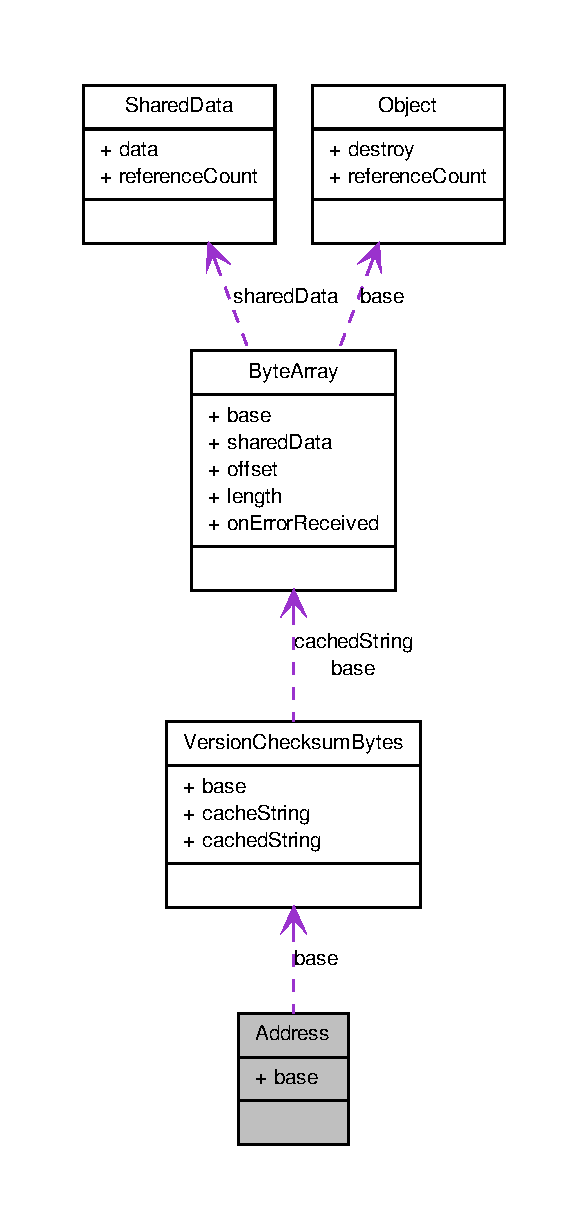
\includegraphics[width=282pt]{struct_address__coll__graph}
\end{center}
\end{figure}
\subsection*{Data Fields}
\begin{DoxyCompactItemize}
\item 
\hyperlink{struct_version_checksum_bytes}{VersionChecksumBytes} \hyperlink{struct_address_acad0c178a202fbaaa57486e58e9cdce2}{base}
\end{DoxyCompactItemize}


\subsection{Detailed Description}
Structure for \hyperlink{struct_address}{Address} objects. 

\begin{DoxySeeAlso}{See also}
\hyperlink{_address_8h}{Address.h} 
\end{DoxySeeAlso}


Definition at line 28 of file Address.h.



\subsection{Field Documentation}
\hypertarget{struct_address_acad0c178a202fbaaa57486e58e9cdce2}{
\index{Address@{Address}!base@{base}}
\index{base@{base}!Address@{Address}}
\subsubsection[{base}]{\setlength{\rightskip}{0pt plus 5cm}{\bf VersionChecksumBytes} {\bf base}}}
\label{struct_address_acad0c178a202fbaaa57486e58e9cdce2}
\hyperlink{struct_version_checksum_bytes}{VersionChecksumBytes} base structure 

Definition at line 29 of file Address.h.



The documentation for this struct was generated from the following file:\begin{DoxyCompactItemize}
\item 
src/Object/VersionChecksumBytes/Address/\hyperlink{_address_8h}{Address.h}\end{DoxyCompactItemize}

\hypertarget{struct_big_int}{
\section{BigInt Struct Reference}
\label{struct_big_int}\index{BigInt@{BigInt}}
}


Contains byte data with the length of this data to represent a large integer. The byte data is in little-\/endian which stores the smallest byte first. On an error data is set to NULL and length is 0.  




{\ttfamily \#include $<$BigInt.h$>$}

\subsection*{Data Fields}
\begin{DoxyCompactItemize}
\item 
uint8\_\-t $\ast$ \hyperlink{struct_big_int_abe222f6d3581e7920dcad5306cc906a8}{data}
\item 
uint8\_\-t \hyperlink{struct_big_int_ab2b3adeb2a67e656ff030b56727fd0ac}{length}
\end{DoxyCompactItemize}


\subsection{Detailed Description}
Contains byte data with the length of this data to represent a large integer. The byte data is in little-\/endian which stores the smallest byte first. On an error data is set to NULL and length is 0. 

Definition at line 19 of file BigInt.h.



\subsection{Field Documentation}
\hypertarget{struct_big_int_abe222f6d3581e7920dcad5306cc906a8}{
\index{BigInt@{BigInt}!data@{data}}
\index{data@{data}!BigInt@{BigInt}}
\subsubsection[{data}]{\setlength{\rightskip}{0pt plus 5cm}uint8\_\-t$\ast$ {\bf data}}}
\label{struct_big_int_abe222f6d3581e7920dcad5306cc906a8}
The byte data. Should be little-\/endian 

Definition at line 20 of file BigInt.h.

\hypertarget{struct_big_int_ab2b3adeb2a67e656ff030b56727fd0ac}{
\index{BigInt@{BigInt}!length@{length}}
\index{length@{length}!BigInt@{BigInt}}
\subsubsection[{length}]{\setlength{\rightskip}{0pt plus 5cm}uint8\_\-t {\bf length}}}
\label{struct_big_int_ab2b3adeb2a67e656ff030b56727fd0ac}
The length of this data in bytes 

Definition at line 21 of file BigInt.h.



The documentation for this struct was generated from the following file:\begin{DoxyCompactItemize}
\item 
src/BigInt/\hyperlink{_big_int_8h}{BigInt.h}\end{DoxyCompactItemize}

\hypertarget{struct_block}{
\section{Block Struct Reference}
\label{struct_block}\index{Block@{Block}}
}


Base class.  




{\ttfamily \#include $<$Block.h$>$}



Collaboration diagram for Block:\nopagebreak
\begin{figure}[H]
\begin{center}
\leavevmode
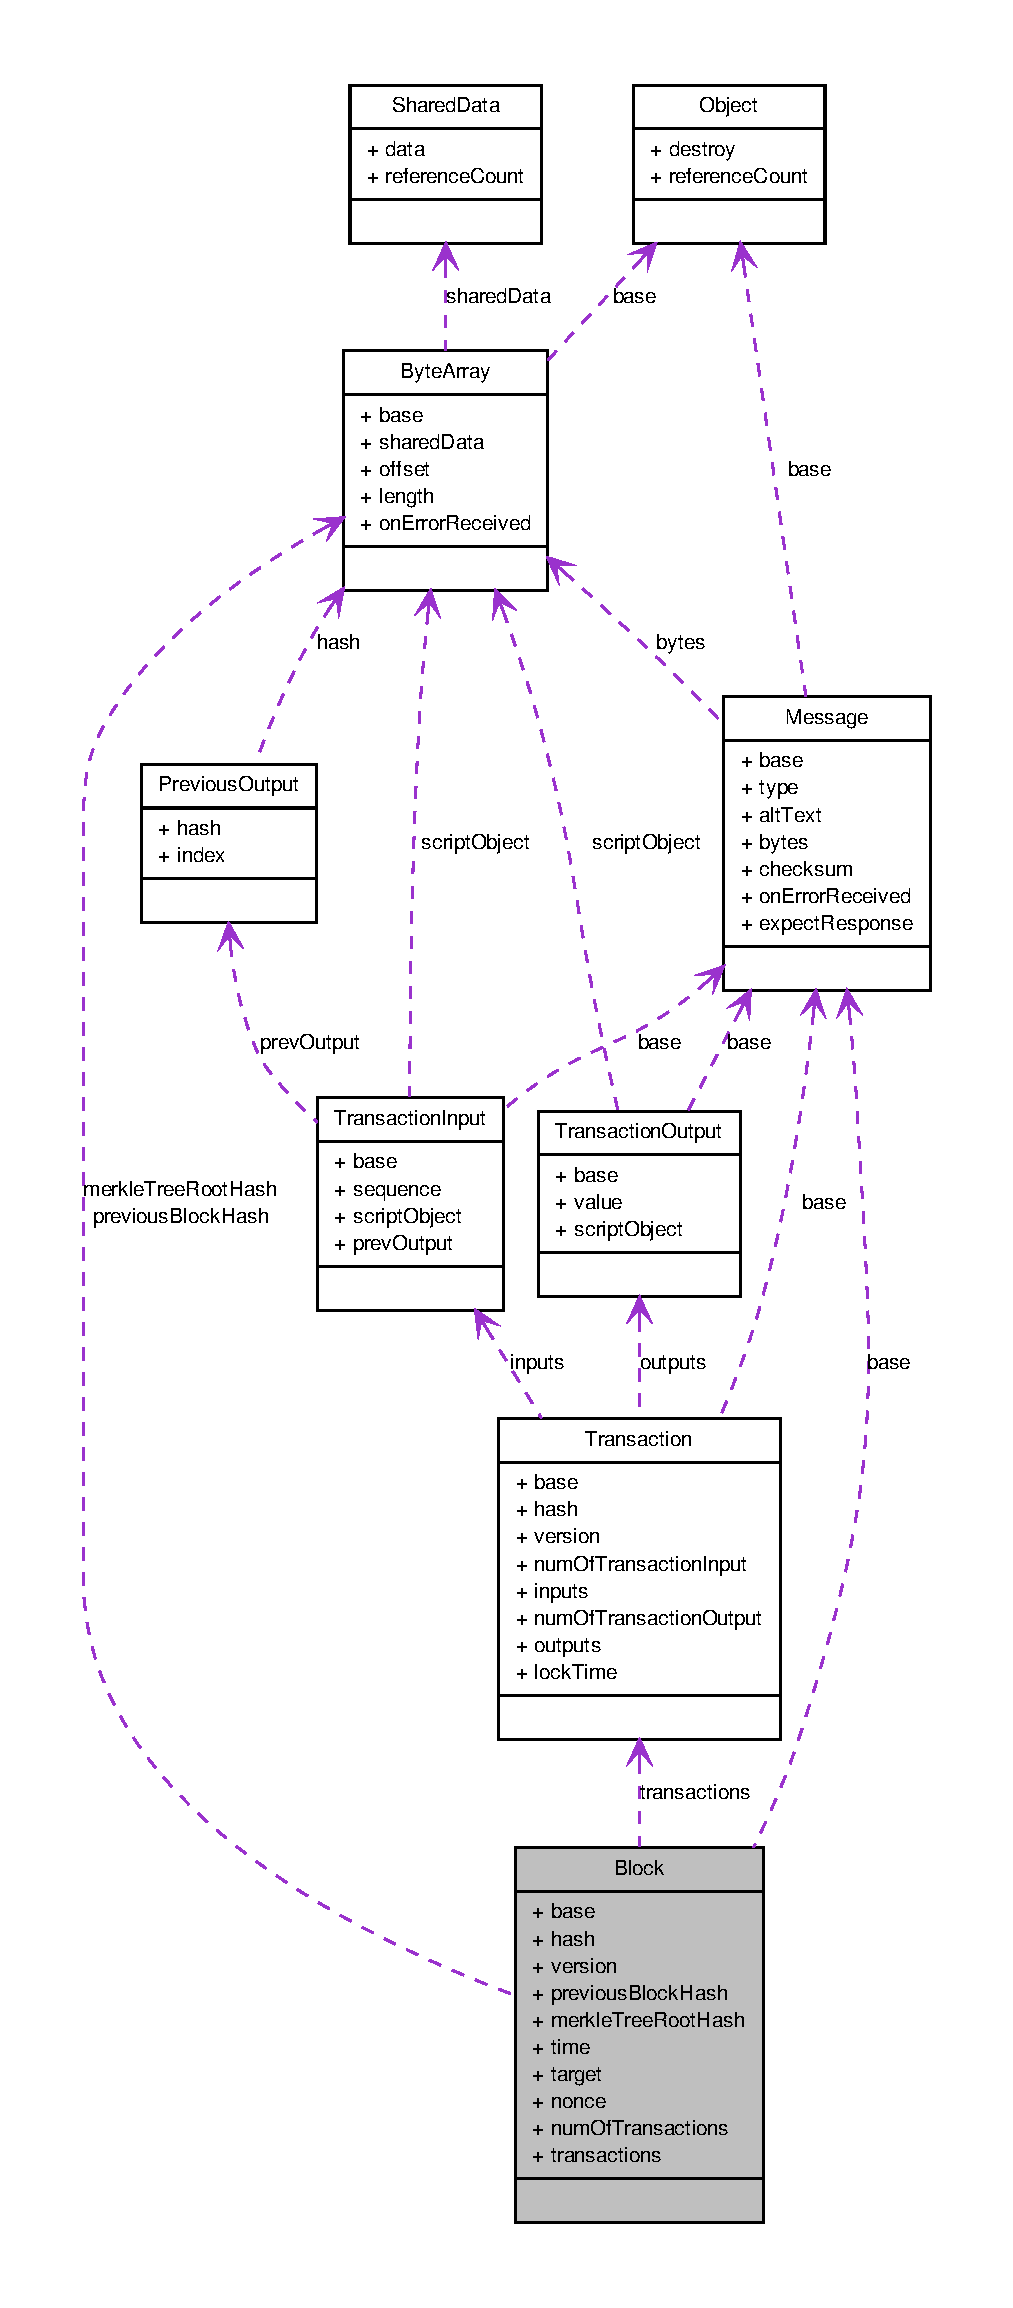
\includegraphics[height=600pt]{struct_block__coll__graph}
\end{center}
\end{figure}
\subsection*{Data Fields}
\begin{DoxyCompactItemize}
\item 
\hyperlink{struct_message}{Message} \hyperlink{struct_block_a8987f797adf70c3e174fd64cc68bc933}{base}
\item 
uint8\_\-t \hyperlink{struct_block_a7ff9da008bf055da1f1ba994c562057d}{hash} \mbox{[}32\mbox{]}
\item 
uint32\_\-t \hyperlink{struct_block_acd99bb05ca015e7d74448acb1deba7ca}{version}
\item 
\hyperlink{struct_byte_array}{ByteArray} $\ast$ \hyperlink{struct_block_ac5cb79d8f66809a5f75592e22db9be2c}{previousBlockHash}
\item 
\hyperlink{struct_byte_array}{ByteArray} $\ast$ \hyperlink{struct_block_a51d24d9b04212dc52192636948a05a4c}{merkleTreeRootHash}
\item 
uint32\_\-t \hyperlink{struct_block_ae73654f333e4363463ad8c594eca1905}{time}
\item 
uint32\_\-t \hyperlink{struct_block_a695e5800ad1fd403c0e72d918eaec97c}{target}
\item 
uint32\_\-t \hyperlink{struct_block_aa2f9785a9d9116cc4592db06375cb887}{nonce}
\item 
uint32\_\-t \hyperlink{struct_block_ac9749ca92207f8d50ecc2b0f904e2424}{numOfTransactions}
\item 
\hyperlink{struct_transaction}{Transaction} $\ast$$\ast$ \hyperlink{struct_block_acf585c1809511c4f5b5366bb2bc2e855}{transactions}
\end{DoxyCompactItemize}


\subsection{Detailed Description}
Base class. 

Definition at line 26 of file Block.h.



\subsection{Field Documentation}
\hypertarget{struct_block_a8987f797adf70c3e174fd64cc68bc933}{
\index{Block@{Block}!base@{base}}
\index{base@{base}!Block@{Block}}
\subsubsection[{base}]{\setlength{\rightskip}{0pt plus 5cm}{\bf Message} {\bf base}}}
\label{struct_block_a8987f797adf70c3e174fd64cc68bc933}
\hyperlink{struct_message}{Message} base structure 

Definition at line 27 of file Block.h.

\hypertarget{struct_block_a7ff9da008bf055da1f1ba994c562057d}{
\index{Block@{Block}!hash@{hash}}
\index{hash@{hash}!Block@{Block}}
\subsubsection[{hash}]{\setlength{\rightskip}{0pt plus 5cm}uint8\_\-t {\bf hash}\mbox{[}32\mbox{]}}}
\label{struct_block_a7ff9da008bf055da1f1ba994c562057d}
The hash for this block. NULL if it needs to be calculated or set. 

Definition at line 28 of file Block.h.

\hypertarget{struct_block_a51d24d9b04212dc52192636948a05a4c}{
\index{Block@{Block}!merkleTreeRootHash@{merkleTreeRootHash}}
\index{merkleTreeRootHash@{merkleTreeRootHash}!Block@{Block}}
\subsubsection[{merkleTreeRootHash}]{\setlength{\rightskip}{0pt plus 5cm}{\bf ByteArray}$\ast$ {\bf merkleTreeRootHash}}}
\label{struct_block_a51d24d9b04212dc52192636948a05a4c}
The merkle tree root hash. To limit the amount of data transferred when synchronizing 

Definition at line 31 of file Block.h.

\hypertarget{struct_block_aa2f9785a9d9116cc4592db06375cb887}{
\index{Block@{Block}!nonce@{nonce}}
\index{nonce@{nonce}!Block@{Block}}
\subsubsection[{nonce}]{\setlength{\rightskip}{0pt plus 5cm}uint32\_\-t {\bf nonce}}}
\label{struct_block_aa2f9785a9d9116cc4592db06375cb887}
A 32-\/bit (4-\/byte) field whose value is set so that the hash of the block will contain a run of zeros in generating blocks 

Definition at line 34 of file Block.h.

\hypertarget{struct_block_ac9749ca92207f8d50ecc2b0f904e2424}{
\index{Block@{Block}!numOfTransactions@{numOfTransactions}}
\index{numOfTransactions@{numOfTransactions}!Block@{Block}}
\subsubsection[{numOfTransactions}]{\setlength{\rightskip}{0pt plus 5cm}uint32\_\-t {\bf numOfTransactions}}}
\label{struct_block_ac9749ca92207f8d50ecc2b0f904e2424}
Number of transactions in the block. 

Definition at line 35 of file Block.h.

\hypertarget{struct_block_ac5cb79d8f66809a5f75592e22db9be2c}{
\index{Block@{Block}!previousBlockHash@{previousBlockHash}}
\index{previousBlockHash@{previousBlockHash}!Block@{Block}}
\subsubsection[{previousBlockHash}]{\setlength{\rightskip}{0pt plus 5cm}{\bf ByteArray}$\ast$ {\bf previousBlockHash}}}
\label{struct_block_ac5cb79d8f66809a5f75592e22db9be2c}
The previous block hash. 

Definition at line 30 of file Block.h.

\hypertarget{struct_block_a695e5800ad1fd403c0e72d918eaec97c}{
\index{Block@{Block}!target@{target}}
\index{target@{target}!Block@{Block}}
\subsubsection[{target}]{\setlength{\rightskip}{0pt plus 5cm}uint32\_\-t {\bf target}}}
\label{struct_block_a695e5800ad1fd403c0e72d918eaec97c}
The compact target representation. 

Definition at line 33 of file Block.h.

\hypertarget{struct_block_ae73654f333e4363463ad8c594eca1905}{
\index{Block@{Block}!time@{time}}
\index{time@{time}!Block@{Block}}
\subsubsection[{time}]{\setlength{\rightskip}{0pt plus 5cm}uint32\_\-t {\bf time}}}
\label{struct_block_ae73654f333e4363463ad8c594eca1905}
Timestamp for the block. The network uses 32 bits. The protocol can be future proofed by detecting overflows when going through the blocks. So if a block's time overflows such that the time is less than the median of the last 10 blocks, the block can be seen by adding the first 32 bits of the network time and finally the timestamp can be tested against the network time. The overflow problem can therefore be fixed by a workaround but it is a shame Satoshi did not use 64 bits. 

Definition at line 32 of file Block.h.

\hypertarget{struct_block_acf585c1809511c4f5b5366bb2bc2e855}{
\index{Block@{Block}!transactions@{transactions}}
\index{transactions@{transactions}!Block@{Block}}
\subsubsection[{transactions}]{\setlength{\rightskip}{0pt plus 5cm}{\bf Transaction}$\ast$$\ast$ {\bf transactions}}}
\label{struct_block_acf585c1809511c4f5b5366bb2bc2e855}
The transactions included in this block. NULL if only the header has been received. 

Definition at line 36 of file Block.h.

\hypertarget{struct_block_acd99bb05ca015e7d74448acb1deba7ca}{
\index{Block@{Block}!version@{version}}
\index{version@{version}!Block@{Block}}
\subsubsection[{version}]{\setlength{\rightskip}{0pt plus 5cm}uint32\_\-t {\bf version}}}
\label{struct_block_acd99bb05ca015e7d74448acb1deba7ca}
block version 

Definition at line 29 of file Block.h.



The documentation for this struct was generated from the following file:\begin{DoxyCompactItemize}
\item 
src/Object/Message/\hyperlink{_block_8h}{Block.h}\end{DoxyCompactItemize}

\hypertarget{struct_block_header}{
\section{BlockHeader Struct Reference}
\label{struct_block_header}\index{BlockHeader@{BlockHeader}}
}


{\ttfamily \#include $<$Protocol.h$>$}

\subsection*{Data Fields}
\begin{DoxyCompactItemize}
\item 
unsigned int \hyperlink{struct_block_header_a5408ac5df4c170828874e1b10b4c35a0}{version}
\item 
char \hyperlink{struct_block_header_a099897f937ebe9e9634c5098e38c7cab}{prevBlock} \mbox{[}32\mbox{]}
\item 
unsigned int \hyperlink{struct_block_header_ad4048a3c215cbfcdc127ada8e0fa5445}{timestamp}
\item 
unsigned int \hyperlink{struct_block_header_aa6da25dae1e7263af226d4b026811d7f}{bits}
\item 
unsigned int \hyperlink{struct_block_header_ad73ee4141a6536b03f4e493b56859e86}{nonce}
\item 
char \hyperlink{struct_block_header_a343e4b09bfd545fad5745f6c48f15b69}{transxCount}
\end{DoxyCompactItemize}


\subsection{Detailed Description}


Definition at line 85 of file Protocol.h.



\subsection{Field Documentation}
\hypertarget{struct_block_header_aa6da25dae1e7263af226d4b026811d7f}{
\index{BlockHeader@{BlockHeader}!bits@{bits}}
\index{bits@{bits}!BlockHeader@{BlockHeader}}
\subsubsection[{bits}]{\setlength{\rightskip}{0pt plus 5cm}unsigned int {\bf bits}}}
\label{struct_block_header_aa6da25dae1e7263af226d4b026811d7f}


Definition at line 90 of file Protocol.h.

\hypertarget{struct_block_header_ad73ee4141a6536b03f4e493b56859e86}{
\index{BlockHeader@{BlockHeader}!nonce@{nonce}}
\index{nonce@{nonce}!BlockHeader@{BlockHeader}}
\subsubsection[{nonce}]{\setlength{\rightskip}{0pt plus 5cm}unsigned int {\bf nonce}}}
\label{struct_block_header_ad73ee4141a6536b03f4e493b56859e86}


Definition at line 91 of file Protocol.h.

\hypertarget{struct_block_header_a099897f937ebe9e9634c5098e38c7cab}{
\index{BlockHeader@{BlockHeader}!prevBlock@{prevBlock}}
\index{prevBlock@{prevBlock}!BlockHeader@{BlockHeader}}
\subsubsection[{prevBlock}]{\setlength{\rightskip}{0pt plus 5cm}char {\bf prevBlock}\mbox{[}32\mbox{]}}}
\label{struct_block_header_a099897f937ebe9e9634c5098e38c7cab}


Definition at line 88 of file Protocol.h.

\hypertarget{struct_block_header_ad4048a3c215cbfcdc127ada8e0fa5445}{
\index{BlockHeader@{BlockHeader}!timestamp@{timestamp}}
\index{timestamp@{timestamp}!BlockHeader@{BlockHeader}}
\subsubsection[{timestamp}]{\setlength{\rightskip}{0pt plus 5cm}unsigned int {\bf timestamp}}}
\label{struct_block_header_ad4048a3c215cbfcdc127ada8e0fa5445}


Definition at line 89 of file Protocol.h.

\hypertarget{struct_block_header_a343e4b09bfd545fad5745f6c48f15b69}{
\index{BlockHeader@{BlockHeader}!transxCount@{transxCount}}
\index{transxCount@{transxCount}!BlockHeader@{BlockHeader}}
\subsubsection[{transxCount}]{\setlength{\rightskip}{0pt plus 5cm}char {\bf transxCount}}}
\label{struct_block_header_a343e4b09bfd545fad5745f6c48f15b69}


Definition at line 92 of file Protocol.h.

\hypertarget{struct_block_header_a5408ac5df4c170828874e1b10b4c35a0}{
\index{BlockHeader@{BlockHeader}!version@{version}}
\index{version@{version}!BlockHeader@{BlockHeader}}
\subsubsection[{version}]{\setlength{\rightskip}{0pt plus 5cm}unsigned int {\bf version}}}
\label{struct_block_header_a5408ac5df4c170828874e1b10b4c35a0}


Definition at line 87 of file Protocol.h.



The documentation for this struct was generated from the following file:\begin{DoxyCompactItemize}
\item 
src/Object/NetworkProtocol/\hyperlink{_protocol_8h}{Protocol.h}\end{DoxyCompactItemize}

\hypertarget{struct_block_headers}{
\section{BlockHeaders Struct Reference}
\label{struct_block_headers}\index{BlockHeaders@{BlockHeaders}}
}


Structure for \hyperlink{struct_block_headers}{BlockHeaders} objects.  




{\ttfamily \#include $<$BlockHeaders.h$>$}



Collaboration diagram for BlockHeaders:
\nopagebreak
\begin{figure}[H]
\begin{center}
\leavevmode
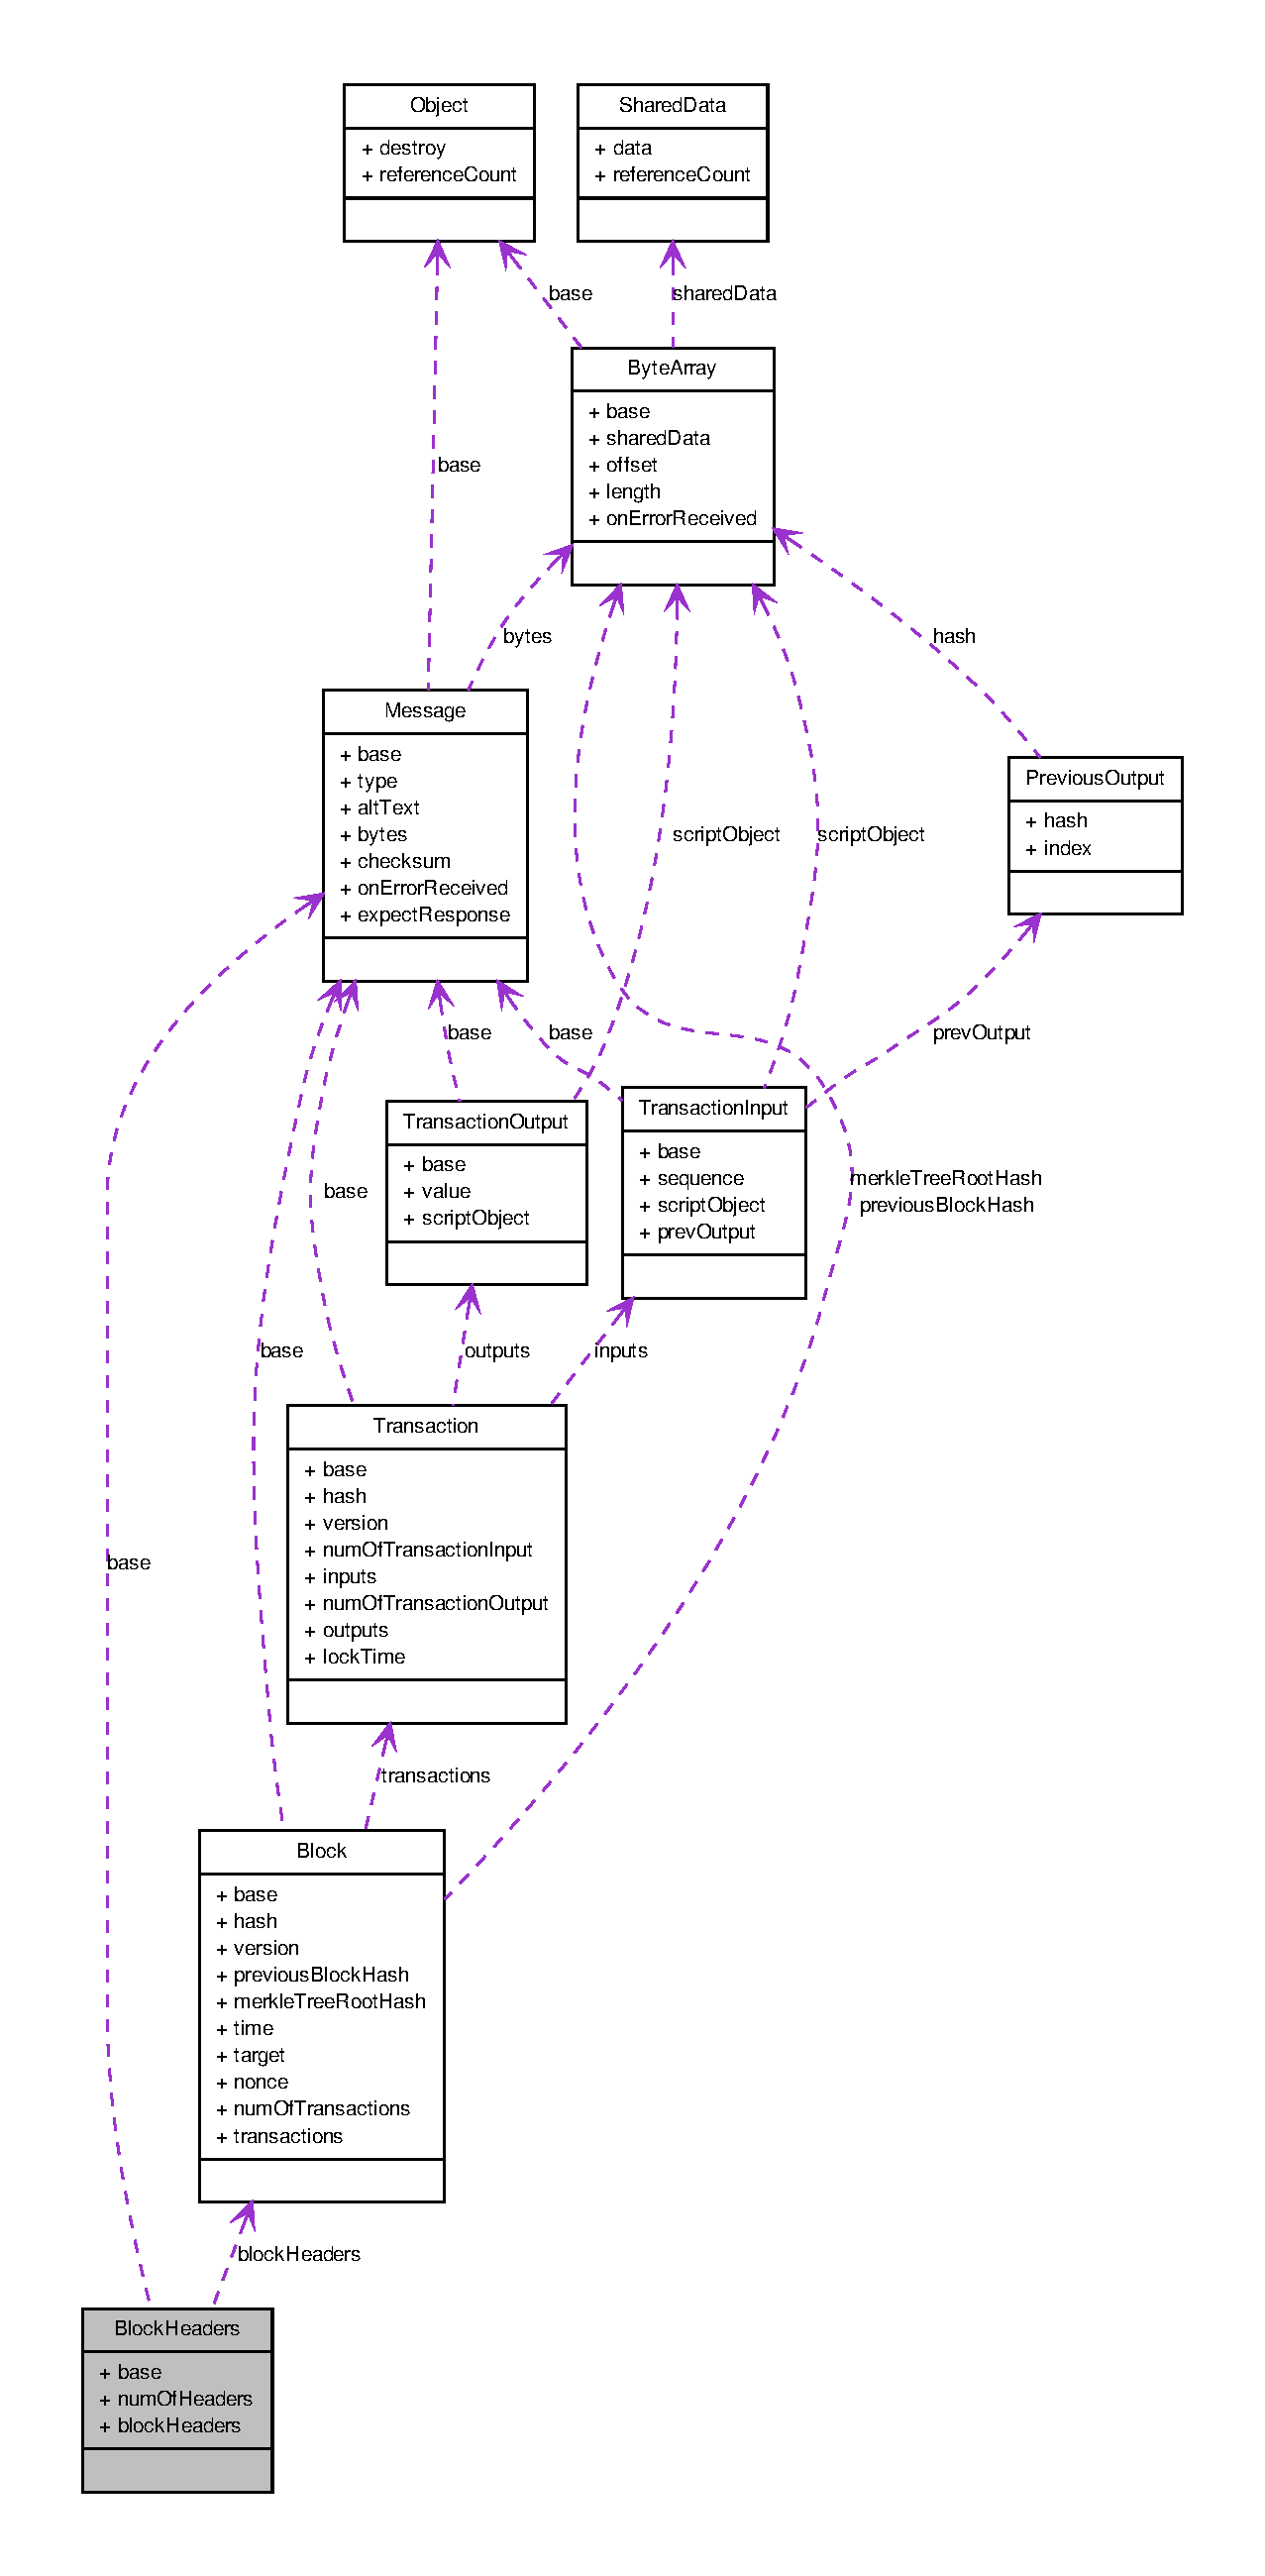
\includegraphics[height=600pt]{struct_block_headers__coll__graph}
\end{center}
\end{figure}
\subsection*{Data Fields}
\begin{DoxyCompactItemize}
\item 
\hyperlink{struct_message}{Message} \hyperlink{struct_block_headers_a8987f797adf70c3e174fd64cc68bc933}{base}
\item 
uint16\_\-t \hyperlink{struct_block_headers_a9cfb2de0666e1e88b621171a97ba801e}{numOfHeaders}
\item 
\hyperlink{struct_block}{Block} $\ast$$\ast$ \hyperlink{struct_block_headers_a33e1983765c280515297ab5b3a4640e0}{blockHeaders}
\end{DoxyCompactItemize}


\subsection{Detailed Description}
Structure for \hyperlink{struct_block_headers}{BlockHeaders} objects. 

\begin{DoxySeeAlso}{See also}
\hyperlink{_block_headers_8h}{BlockHeaders.h} 
\end{DoxySeeAlso}


Definition at line 23 of file BlockHeaders.h.



\subsection{Field Documentation}
\hypertarget{struct_block_headers_a8987f797adf70c3e174fd64cc68bc933}{
\index{BlockHeaders@{BlockHeaders}!base@{base}}
\index{base@{base}!BlockHeaders@{BlockHeaders}}
\subsubsection[{base}]{\setlength{\rightskip}{0pt plus 5cm}{\bf Message} {\bf base}}}
\label{struct_block_headers_a8987f797adf70c3e174fd64cc68bc933}
\hyperlink{struct_message}{Message} base structure 

Definition at line 24 of file BlockHeaders.h.

\hypertarget{struct_block_headers_a33e1983765c280515297ab5b3a4640e0}{
\index{BlockHeaders@{BlockHeaders}!blockHeaders@{blockHeaders}}
\index{blockHeaders@{blockHeaders}!BlockHeaders@{BlockHeaders}}
\subsubsection[{blockHeaders}]{\setlength{\rightskip}{0pt plus 5cm}{\bf Block}$\ast$$\ast$ {\bf blockHeaders}}}
\label{struct_block_headers_a33e1983765c280515297ab5b3a4640e0}
The block headers as \hyperlink{struct_block}{Block} objects with no transactions. The number of transactions is given however. 

Definition at line 26 of file BlockHeaders.h.

\hypertarget{struct_block_headers_a9cfb2de0666e1e88b621171a97ba801e}{
\index{BlockHeaders@{BlockHeaders}!numOfHeaders@{numOfHeaders}}
\index{numOfHeaders@{numOfHeaders}!BlockHeaders@{BlockHeaders}}
\subsubsection[{numOfHeaders}]{\setlength{\rightskip}{0pt plus 5cm}uint16\_\-t {\bf numOfHeaders}}}
\label{struct_block_headers_a9cfb2de0666e1e88b621171a97ba801e}
The number of headers. 

Definition at line 25 of file BlockHeaders.h.



The documentation for this struct was generated from the following file:\begin{DoxyCompactItemize}
\item 
src/Object/Message/\hyperlink{_block_headers_8h}{BlockHeaders.h}\end{DoxyCompactItemize}

\hypertarget{struct_block_spck}{
\section{BlockSpck Struct Reference}
\label{struct_block_spck}\index{BlockSpck@{BlockSpck}}
}


{\ttfamily \#include $<$Protocol.h$>$}

\subsection*{Data Fields}
\begin{DoxyCompactItemize}
\item 
unsigned int \hyperlink{struct_block_spck_a5408ac5df4c170828874e1b10b4c35a0}{version}
\item 
unsigned int \hyperlink{struct_block_spck_a8063bd9a895b61caa30d0ca876a6e300}{startCount}
\item 
char \hyperlink{struct_block_spck_a95789ecf55183a47b1668d549ba4a927}{blockLocatorHashes} \mbox{[}32\mbox{]}
\item 
char \hyperlink{struct_block_spck_aa16ea670ce42c626f461fc49f74ddcd3}{hashStop} \mbox{[}32\mbox{]}
\end{DoxyCompactItemize}


\subsection{Detailed Description}


Definition at line 127 of file Protocol.h.



\subsection{Field Documentation}
\hypertarget{struct_block_spck_a95789ecf55183a47b1668d549ba4a927}{
\index{BlockSpck@{BlockSpck}!blockLocatorHashes@{blockLocatorHashes}}
\index{blockLocatorHashes@{blockLocatorHashes}!BlockSpck@{BlockSpck}}
\subsubsection[{blockLocatorHashes}]{\setlength{\rightskip}{0pt plus 5cm}char {\bf blockLocatorHashes}\mbox{[}32\mbox{]}}}
\label{struct_block_spck_a95789ecf55183a47b1668d549ba4a927}


Definition at line 130 of file Protocol.h.

\hypertarget{struct_block_spck_aa16ea670ce42c626f461fc49f74ddcd3}{
\index{BlockSpck@{BlockSpck}!hashStop@{hashStop}}
\index{hashStop@{hashStop}!BlockSpck@{BlockSpck}}
\subsubsection[{hashStop}]{\setlength{\rightskip}{0pt plus 5cm}char {\bf hashStop}\mbox{[}32\mbox{]}}}
\label{struct_block_spck_aa16ea670ce42c626f461fc49f74ddcd3}


Definition at line 131 of file Protocol.h.

\hypertarget{struct_block_spck_a8063bd9a895b61caa30d0ca876a6e300}{
\index{BlockSpck@{BlockSpck}!startCount@{startCount}}
\index{startCount@{startCount}!BlockSpck@{BlockSpck}}
\subsubsection[{startCount}]{\setlength{\rightskip}{0pt plus 5cm}unsigned int {\bf startCount}}}
\label{struct_block_spck_a8063bd9a895b61caa30d0ca876a6e300}


Definition at line 129 of file Protocol.h.

\hypertarget{struct_block_spck_a5408ac5df4c170828874e1b10b4c35a0}{
\index{BlockSpck@{BlockSpck}!version@{version}}
\index{version@{version}!BlockSpck@{BlockSpck}}
\subsubsection[{version}]{\setlength{\rightskip}{0pt plus 5cm}unsigned int {\bf version}}}
\label{struct_block_spck_a5408ac5df4c170828874e1b10b4c35a0}


Definition at line 128 of file Protocol.h.



The documentation for this struct was generated from the following file:\begin{DoxyCompactItemize}
\item 
src/Object/NetworkProtocol/\hyperlink{_protocol_8h}{Protocol.h}\end{DoxyCompactItemize}

\hypertarget{struct_byte_array}{
\section{ByteArray Struct Reference}
\label{struct_byte_array}\index{ByteArray@{ByteArray}}
}


Structure for \hyperlink{struct_byte_array}{ByteArray} objects.  




{\ttfamily \#include $<$ByteArray.h$>$}



Collaboration diagram for ByteArray:\nopagebreak
\begin{figure}[H]
\begin{center}
\leavevmode
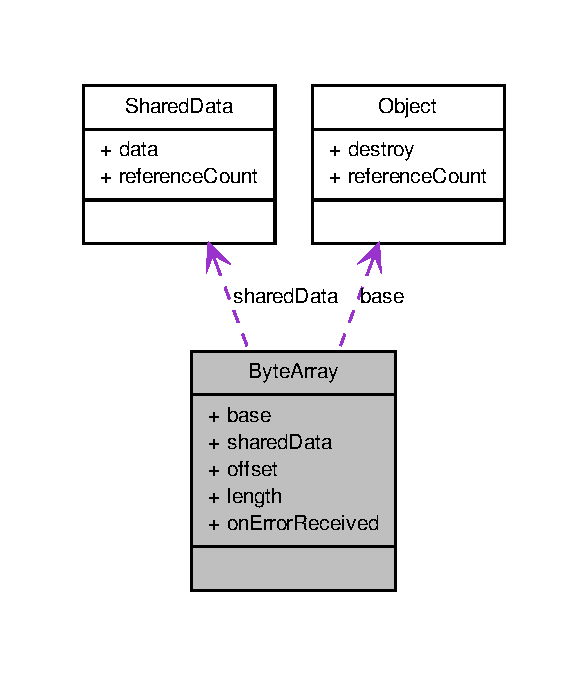
\includegraphics[width=282pt]{struct_byte_array__coll__graph}
\end{center}
\end{figure}
\subsection*{Data Fields}
\begin{DoxyCompactItemize}
\item 
\hyperlink{struct_object}{Object} \hyperlink{struct_byte_array_a23cf4ef56ba22bed625eab08d6361fa7}{base}
\item 
\hyperlink{struct_shared_data}{SharedData} $\ast$ \hyperlink{struct_byte_array_a0a0e8cb81138e26f1a3dba7c425f71e1}{sharedData}
\item 
uint32\_\-t \hyperlink{struct_byte_array_a894bdfa2d603d8343f8ef01dda6fcd23}{offset}
\item 
uint32\_\-t \hyperlink{struct_byte_array_aebb70c2aab3407a9f05334c47131a43b}{length}
\item 
void($\ast$ \hyperlink{struct_byte_array_a3c8af4f580f3041d046b7581f89a9695}{onErrorReceived} )(\hyperlink{_constants_8h_a2c3e4bb40f36b262a5214e2da2bca9c5}{Error} error, char $\ast$,...)
\end{DoxyCompactItemize}


\subsection{Detailed Description}
Structure for \hyperlink{struct_byte_array}{ByteArray} objects. 

\begin{DoxySeeAlso}{See also}
\hyperlink{_byte_array_8h}{ByteArray.h} 
\end{DoxySeeAlso}


Definition at line 29 of file ByteArray.h.



\subsection{Field Documentation}
\hypertarget{struct_byte_array_a23cf4ef56ba22bed625eab08d6361fa7}{
\index{ByteArray@{ByteArray}!base@{base}}
\index{base@{base}!ByteArray@{ByteArray}}
\subsubsection[{base}]{\setlength{\rightskip}{0pt plus 5cm}{\bf Object} {\bf base}}}
\label{struct_byte_array_a23cf4ef56ba22bed625eab08d6361fa7}
\hyperlink{struct_object}{Object} base structure 

Definition at line 30 of file ByteArray.h.

\hypertarget{struct_byte_array_aebb70c2aab3407a9f05334c47131a43b}{
\index{ByteArray@{ByteArray}!length@{length}}
\index{length@{length}!ByteArray@{ByteArray}}
\subsubsection[{length}]{\setlength{\rightskip}{0pt plus 5cm}uint32\_\-t {\bf length}}}
\label{struct_byte_array_aebb70c2aab3407a9f05334c47131a43b}
Length of byte array. Set to \_\-BYTE\_\-ARRAY\_\-UNKNOWN\_\-LENGTH if unknown. 

Definition at line 33 of file ByteArray.h.

\hypertarget{struct_byte_array_a894bdfa2d603d8343f8ef01dda6fcd23}{
\index{ByteArray@{ByteArray}!offset@{offset}}
\index{offset@{offset}!ByteArray@{ByteArray}}
\subsubsection[{offset}]{\setlength{\rightskip}{0pt plus 5cm}uint32\_\-t {\bf offset}}}
\label{struct_byte_array_a894bdfa2d603d8343f8ef01dda6fcd23}
Offset from the beginning of the byte data to the beginning of this array 

Definition at line 32 of file ByteArray.h.

\hypertarget{struct_byte_array_a3c8af4f580f3041d046b7581f89a9695}{
\index{ByteArray@{ByteArray}!onErrorReceived@{onErrorReceived}}
\index{onErrorReceived@{onErrorReceived}!ByteArray@{ByteArray}}
\subsubsection[{onErrorReceived}]{\setlength{\rightskip}{0pt plus 5cm}void($\ast$ {\bf onErrorReceived})({\bf Error} error, char $\ast$,...)}}
\label{struct_byte_array_a3c8af4f580f3041d046b7581f89a9695}


Definition at line 34 of file ByteArray.h.

\hypertarget{struct_byte_array_a0a0e8cb81138e26f1a3dba7c425f71e1}{
\index{ByteArray@{ByteArray}!sharedData@{sharedData}}
\index{sharedData@{sharedData}!ByteArray@{ByteArray}}
\subsubsection[{sharedData}]{\setlength{\rightskip}{0pt plus 5cm}{\bf SharedData}$\ast$ {\bf sharedData}}}
\label{struct_byte_array_a0a0e8cb81138e26f1a3dba7c425f71e1}
Underlying byte data 

Definition at line 31 of file ByteArray.h.



The documentation for this struct was generated from the following file:\begin{DoxyCompactItemize}
\item 
src/Object/\hyperlink{_byte_array_8h}{ByteArray.h}\end{DoxyCompactItemize}

\hypertarget{struct_chain_descriptor}{
\section{ChainDescriptor Struct Reference}
\label{struct_chain_descriptor}\index{ChainDescriptor@{ChainDescriptor}}
}


Structure for \hyperlink{struct_chain_descriptor}{ChainDescriptor} objects.  




{\ttfamily \#include $<$ChainDescriptor.h$>$}



Collaboration diagram for ChainDescriptor:
\nopagebreak
\begin{figure}[H]
\begin{center}
\leavevmode
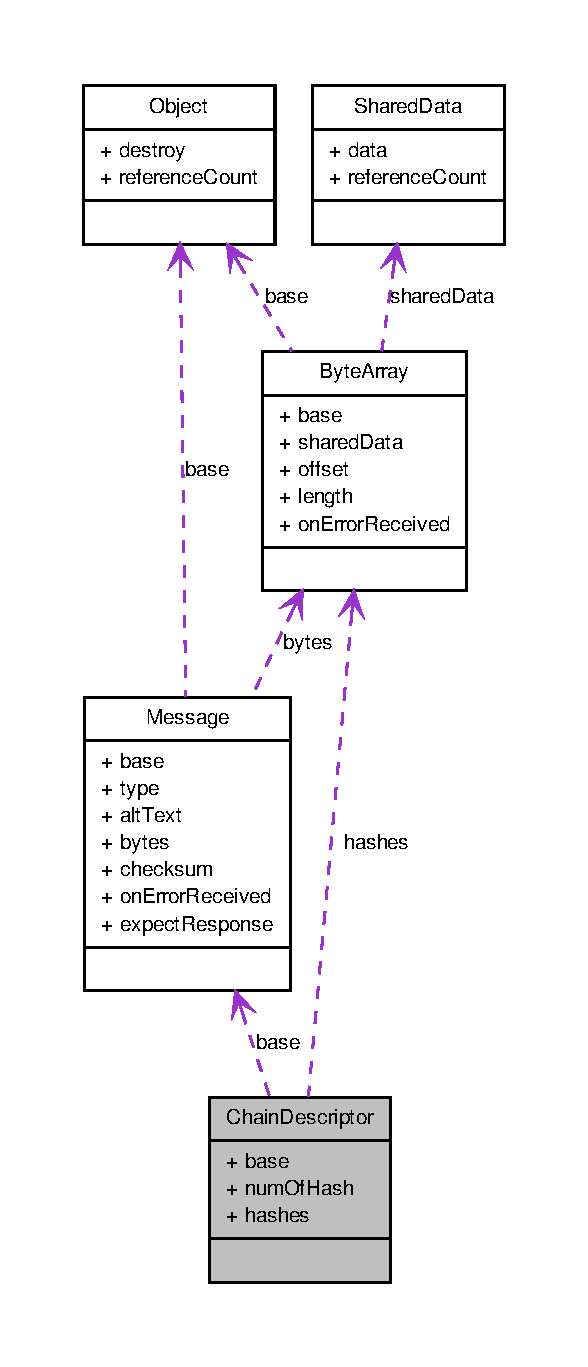
\includegraphics[height=600pt]{struct_chain_descriptor__coll__graph}
\end{center}
\end{figure}
\subsection*{Data Fields}
\begin{DoxyCompactItemize}
\item 
\hyperlink{struct_message}{Message} \hyperlink{struct_chain_descriptor_a8987f797adf70c3e174fd64cc68bc933}{base}
\item 
uint16\_\-t \hyperlink{struct_chain_descriptor_a2a73cb6d678dd0457074398eb7c27584}{numOfHash}
\item 
\hyperlink{struct_byte_array}{ByteArray} $\ast$$\ast$ \hyperlink{struct_chain_descriptor_accd2c3f99c875e8657d976fc264c7fc6}{hashes}
\end{DoxyCompactItemize}


\subsection{Detailed Description}
Structure for \hyperlink{struct_chain_descriptor}{ChainDescriptor} objects. 

\begin{DoxySeeAlso}{See also}
\hyperlink{_chain_descriptor_8h}{ChainDescriptor.h} 
\end{DoxySeeAlso}


Definition at line 22 of file ChainDescriptor.h.



\subsection{Field Documentation}
\hypertarget{struct_chain_descriptor_a8987f797adf70c3e174fd64cc68bc933}{
\index{ChainDescriptor@{ChainDescriptor}!base@{base}}
\index{base@{base}!ChainDescriptor@{ChainDescriptor}}
\subsubsection[{base}]{\setlength{\rightskip}{0pt plus 5cm}{\bf Message} {\bf base}}}
\label{struct_chain_descriptor_a8987f797adf70c3e174fd64cc68bc933}
\hyperlink{struct_message}{Message} base structure 

Definition at line 23 of file ChainDescriptor.h.

\hypertarget{struct_chain_descriptor_accd2c3f99c875e8657d976fc264c7fc6}{
\index{ChainDescriptor@{ChainDescriptor}!hashes@{hashes}}
\index{hashes@{hashes}!ChainDescriptor@{ChainDescriptor}}
\subsubsection[{hashes}]{\setlength{\rightskip}{0pt plus 5cm}{\bf ByteArray}$\ast$$\ast$ {\bf hashes}}}
\label{struct_chain_descriptor_accd2c3f99c875e8657d976fc264c7fc6}
Hashes used to describe the block chain. This should contain hashes in the blockchain but not all of them. The maximum allowed is 500. The usual behaviour is to have the 10 last block hashes and then each hash below those going down to the genesis block has a gap that doubles (See \href{https://en.bitcoin.it/wiki/Protocol_specification#getblocks}{\tt https://en.bitcoin.it/wiki/Protocol\_\-specification\#getblocks} ). The newest block hashes should come first. This should be NULL if empty. The \hyperlink{struct_get_blocks}{GetBlocks} object will release each \hyperlink{struct_byte_array}{ByteArray} and free the array when the object is freed. 

Definition at line 25 of file ChainDescriptor.h.

\hypertarget{struct_chain_descriptor_a2a73cb6d678dd0457074398eb7c27584}{
\index{ChainDescriptor@{ChainDescriptor}!numOfHash@{numOfHash}}
\index{numOfHash@{numOfHash}!ChainDescriptor@{ChainDescriptor}}
\subsubsection[{numOfHash}]{\setlength{\rightskip}{0pt plus 5cm}uint16\_\-t {\bf numOfHash}}}
\label{struct_chain_descriptor_a2a73cb6d678dd0457074398eb7c27584}
Number of block hashes to describe the block chain. Up to 500. 

Definition at line 24 of file ChainDescriptor.h.



The documentation for this struct was generated from the following file:\begin{DoxyCompactItemize}
\item 
src/Object/Message/\hyperlink{_chain_descriptor_8h}{ChainDescriptor.h}\end{DoxyCompactItemize}

\hypertarget{struct_cmd_addr}{
\section{CmdAddr Struct Reference}
\label{struct_cmd_addr}\index{CmdAddr@{CmdAddr}}
}


{\ttfamily \#include $<$Commands.h$>$}



Collaboration diagram for CmdAddr:\nopagebreak
\begin{figure}[H]
\begin{center}
\leavevmode
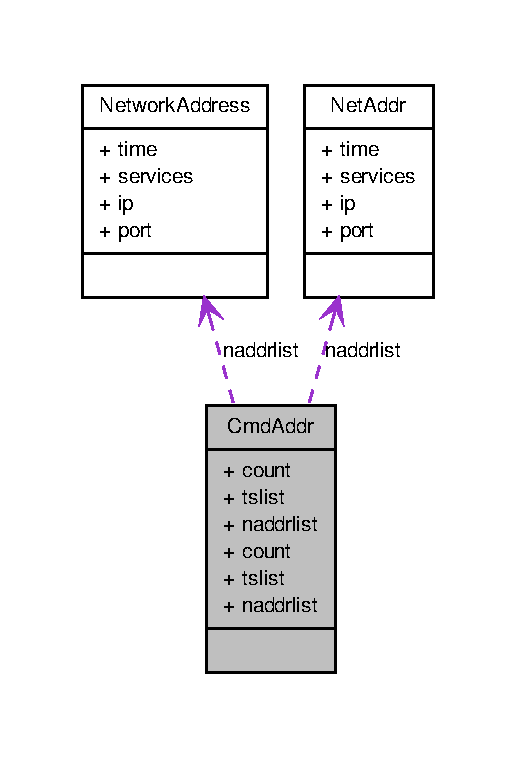
\includegraphics[width=248pt]{struct_cmd_addr__coll__graph}
\end{center}
\end{figure}
\subsection*{Data Fields}
\begin{DoxyCompactItemize}
\item 
uint32\_\-t \hyperlink{struct_cmd_addr_a86988a65e0d3ece7990c032c159786d6}{count}
\item 
uint32\_\-t $\ast$ \hyperlink{struct_cmd_addr_a690496cb0763044d995a40b46e8f7d32}{tslist}
\item 
struct \hyperlink{struct_network_address}{NetworkAddress} $\ast$ \hyperlink{struct_cmd_addr_a39e0b80e0408806939286dfb40cfd081}{naddrlist}
\item 
unsigned int \hyperlink{struct_cmd_addr_a16ff2d8e15ade4948398b0aeb80124a8}{count}
\item 
unsigned int $\ast$ \hyperlink{struct_cmd_addr_af8bd06c27cd9c81c75e60853080e7e7e}{tslist}
\item 
struct \hyperlink{struct_net_addr}{NetAddr} $\ast$ \hyperlink{struct_cmd_addr_a65d94e910a546e06b09f1daa9978e52c}{naddrlist}
\end{DoxyCompactItemize}


\subsection{Detailed Description}


Definition at line 101 of file Commands.h.



\subsection{Field Documentation}
\hypertarget{struct_cmd_addr_a86988a65e0d3ece7990c032c159786d6}{
\index{CmdAddr@{CmdAddr}!count@{count}}
\index{count@{count}!CmdAddr@{CmdAddr}}
\subsubsection[{count}]{\setlength{\rightskip}{0pt plus 5cm}uint32\_\-t {\bf count}}}
\label{struct_cmd_addr_a86988a65e0d3ece7990c032c159786d6}


Definition at line 104 of file Commands.h.

\hypertarget{struct_cmd_addr_a16ff2d8e15ade4948398b0aeb80124a8}{
\index{CmdAddr@{CmdAddr}!count@{count}}
\index{count@{count}!CmdAddr@{CmdAddr}}
\subsubsection[{count}]{\setlength{\rightskip}{0pt plus 5cm}unsigned int {\bf count}}}
\label{struct_cmd_addr_a16ff2d8e15ade4948398b0aeb80124a8}


Definition at line 101 of file Protocol.h.

\hypertarget{struct_cmd_addr_a65d94e910a546e06b09f1daa9978e52c}{
\index{CmdAddr@{CmdAddr}!naddrlist@{naddrlist}}
\index{naddrlist@{naddrlist}!CmdAddr@{CmdAddr}}
\subsubsection[{naddrlist}]{\setlength{\rightskip}{0pt plus 5cm}struct {\bf NetAddr}$\ast$ {\bf naddrlist}}}
\label{struct_cmd_addr_a65d94e910a546e06b09f1daa9978e52c}


Definition at line 106 of file Protocol.h.

\hypertarget{struct_cmd_addr_a39e0b80e0408806939286dfb40cfd081}{
\index{CmdAddr@{CmdAddr}!naddrlist@{naddrlist}}
\index{naddrlist@{naddrlist}!CmdAddr@{CmdAddr}}
\subsubsection[{naddrlist}]{\setlength{\rightskip}{0pt plus 5cm}struct {\bf NetworkAddress}$\ast$ {\bf naddrlist}}}
\label{struct_cmd_addr_a39e0b80e0408806939286dfb40cfd081}


Definition at line 109 of file Commands.h.

\hypertarget{struct_cmd_addr_a690496cb0763044d995a40b46e8f7d32}{
\index{CmdAddr@{CmdAddr}!tslist@{tslist}}
\index{tslist@{tslist}!CmdAddr@{CmdAddr}}
\subsubsection[{tslist}]{\setlength{\rightskip}{0pt plus 5cm}uint32\_\-t$\ast$ {\bf tslist}}}
\label{struct_cmd_addr_a690496cb0763044d995a40b46e8f7d32}


Definition at line 107 of file Commands.h.

\hypertarget{struct_cmd_addr_af8bd06c27cd9c81c75e60853080e7e7e}{
\index{CmdAddr@{CmdAddr}!tslist@{tslist}}
\index{tslist@{tslist}!CmdAddr@{CmdAddr}}
\subsubsection[{tslist}]{\setlength{\rightskip}{0pt plus 5cm}unsigned int$\ast$ {\bf tslist}}}
\label{struct_cmd_addr_af8bd06c27cd9c81c75e60853080e7e7e}


Definition at line 104 of file Protocol.h.



The documentation for this struct was generated from the following files:\begin{DoxyCompactItemize}
\item 
src/Object/NetworkProtocol/\hyperlink{_commands_8h}{Commands.h}\item 
src/Object/NetworkProtocol/\hyperlink{_protocol_8h}{Protocol.h}\end{DoxyCompactItemize}

\hypertarget{struct_cmd_alert}{
\section{CmdAlert Struct Reference}
\label{struct_cmd_alert}\index{CmdAlert@{CmdAlert}}
}


{\ttfamily \#include $<$Commands.h$>$}



\subsection{Detailed Description}


Definition at line 188 of file Commands.h.



The documentation for this struct was generated from the following file:\begin{DoxyCompactItemize}
\item 
src/Object/NetworkProtocol/\hyperlink{_commands_8h}{Commands.h}\end{DoxyCompactItemize}

\hypertarget{struct_cmd_block}{
\section{CmdBlock Struct Reference}
\label{struct_cmd_block}\index{CmdBlock@{CmdBlock}}
}


{\ttfamily \#include $<$Protocol.h$>$}



Collaboration diagram for CmdBlock:\nopagebreak
\begin{figure}[H]
\begin{center}
\leavevmode
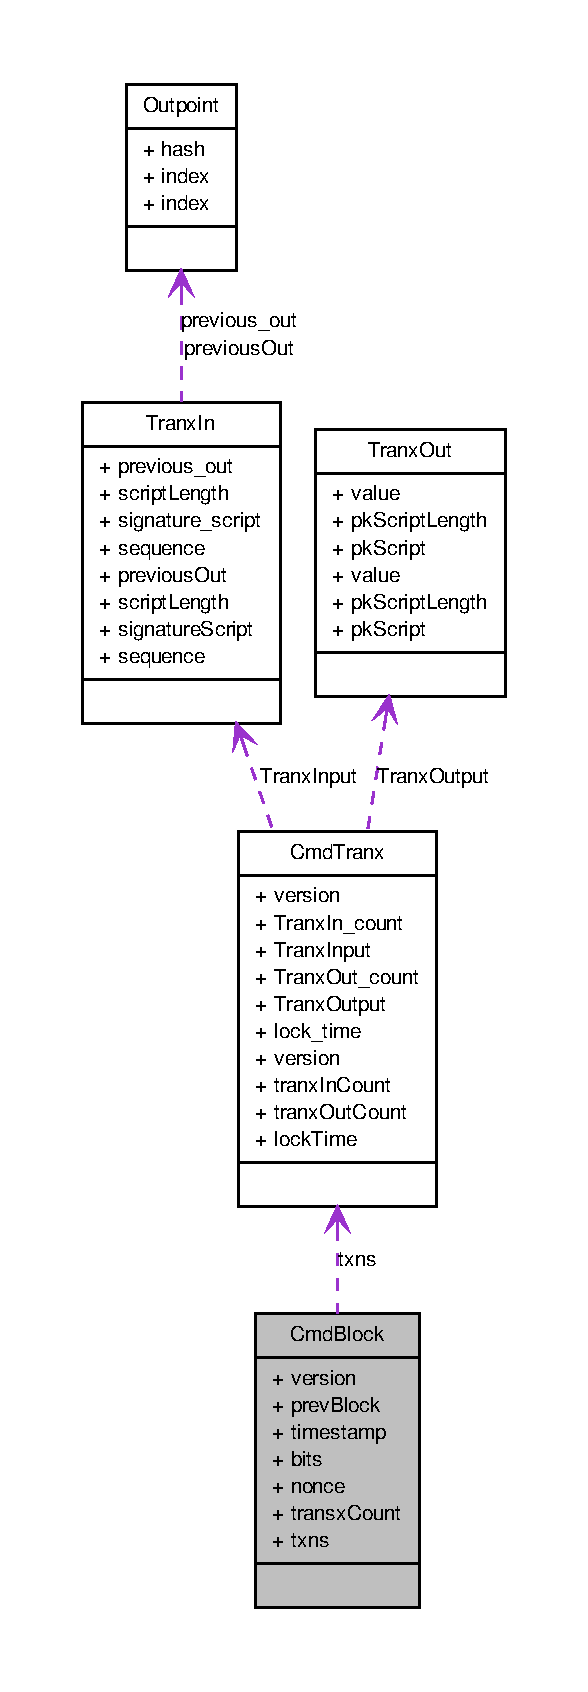
\includegraphics[height=600pt]{struct_cmd_block__coll__graph}
\end{center}
\end{figure}
\subsection*{Data Fields}
\begin{DoxyCompactItemize}
\item 
unsigned int \hyperlink{struct_cmd_block_a5408ac5df4c170828874e1b10b4c35a0}{version}
\item 
char \hyperlink{struct_cmd_block_a099897f937ebe9e9634c5098e38c7cab}{prevBlock} \mbox{[}32\mbox{]}
\item 
unsigned int \hyperlink{struct_cmd_block_ad4048a3c215cbfcdc127ada8e0fa5445}{timestamp}
\item 
unsigned int \hyperlink{struct_cmd_block_aa6da25dae1e7263af226d4b026811d7f}{bits}
\item 
unsigned int \hyperlink{struct_cmd_block_ad73ee4141a6536b03f4e493b56859e86}{nonce}
\item 
unsigned int \hyperlink{struct_cmd_block_a74334da90ccc4ebde303deecbe77f9dd}{transxCount}
\item 
struct \hyperlink{struct_cmd_tranx}{CmdTranx} $\ast$ \hyperlink{struct_cmd_block_a50142212678034606e6aa3304ea06fb7}{txns}
\end{DoxyCompactItemize}


\subsection{Detailed Description}


Definition at line 183 of file Protocol.h.



\subsection{Field Documentation}
\hypertarget{struct_cmd_block_aa6da25dae1e7263af226d4b026811d7f}{
\index{CmdBlock@{CmdBlock}!bits@{bits}}
\index{bits@{bits}!CmdBlock@{CmdBlock}}
\subsubsection[{bits}]{\setlength{\rightskip}{0pt plus 5cm}unsigned int {\bf bits}}}
\label{struct_cmd_block_aa6da25dae1e7263af226d4b026811d7f}


Definition at line 187 of file Protocol.h.

\hypertarget{struct_cmd_block_ad73ee4141a6536b03f4e493b56859e86}{
\index{CmdBlock@{CmdBlock}!nonce@{nonce}}
\index{nonce@{nonce}!CmdBlock@{CmdBlock}}
\subsubsection[{nonce}]{\setlength{\rightskip}{0pt plus 5cm}unsigned int {\bf nonce}}}
\label{struct_cmd_block_ad73ee4141a6536b03f4e493b56859e86}


Definition at line 188 of file Protocol.h.

\hypertarget{struct_cmd_block_a099897f937ebe9e9634c5098e38c7cab}{
\index{CmdBlock@{CmdBlock}!prevBlock@{prevBlock}}
\index{prevBlock@{prevBlock}!CmdBlock@{CmdBlock}}
\subsubsection[{prevBlock}]{\setlength{\rightskip}{0pt plus 5cm}char {\bf prevBlock}\mbox{[}32\mbox{]}}}
\label{struct_cmd_block_a099897f937ebe9e9634c5098e38c7cab}


Definition at line 185 of file Protocol.h.

\hypertarget{struct_cmd_block_ad4048a3c215cbfcdc127ada8e0fa5445}{
\index{CmdBlock@{CmdBlock}!timestamp@{timestamp}}
\index{timestamp@{timestamp}!CmdBlock@{CmdBlock}}
\subsubsection[{timestamp}]{\setlength{\rightskip}{0pt plus 5cm}unsigned int {\bf timestamp}}}
\label{struct_cmd_block_ad4048a3c215cbfcdc127ada8e0fa5445}


Definition at line 186 of file Protocol.h.

\hypertarget{struct_cmd_block_a74334da90ccc4ebde303deecbe77f9dd}{
\index{CmdBlock@{CmdBlock}!transxCount@{transxCount}}
\index{transxCount@{transxCount}!CmdBlock@{CmdBlock}}
\subsubsection[{transxCount}]{\setlength{\rightskip}{0pt plus 5cm}unsigned int {\bf transxCount}}}
\label{struct_cmd_block_a74334da90ccc4ebde303deecbe77f9dd}


Definition at line 189 of file Protocol.h.

\hypertarget{struct_cmd_block_a50142212678034606e6aa3304ea06fb7}{
\index{CmdBlock@{CmdBlock}!txns@{txns}}
\index{txns@{txns}!CmdBlock@{CmdBlock}}
\subsubsection[{txns}]{\setlength{\rightskip}{0pt plus 5cm}struct {\bf CmdTranx}$\ast$ {\bf txns}}}
\label{struct_cmd_block_a50142212678034606e6aa3304ea06fb7}


Definition at line 190 of file Protocol.h.

\hypertarget{struct_cmd_block_a5408ac5df4c170828874e1b10b4c35a0}{
\index{CmdBlock@{CmdBlock}!version@{version}}
\index{version@{version}!CmdBlock@{CmdBlock}}
\subsubsection[{version}]{\setlength{\rightskip}{0pt plus 5cm}unsigned int {\bf version}}}
\label{struct_cmd_block_a5408ac5df4c170828874e1b10b4c35a0}


Definition at line 184 of file Protocol.h.



The documentation for this struct was generated from the following file:\begin{DoxyCompactItemize}
\item 
src/Object/NetworkProtocol/\hyperlink{_protocol_8h}{Protocol.h}\end{DoxyCompactItemize}

\hypertarget{struct_cmdblock}{
\section{Cmdblock Struct Reference}
\label{struct_cmdblock}\index{Cmdblock@{Cmdblock}}
}


{\ttfamily \#include $<$Commands.h$>$}

\subsection*{Data Fields}
\begin{DoxyCompactItemize}
\item 
uint32\_\-t \hyperlink{struct_cmdblock_acd99bb05ca015e7d74448acb1deba7ca}{version}
\item 
char \hyperlink{struct_cmdblock_a742f80039bbe773ec691c1ce0ae01f95}{prev\_\-block} \mbox{[}32\mbox{]}
\item 
char \hyperlink{struct_cmdblock_a6a88b5c7b1ef72e9ba761f9f8d4525a4}{markle\_\-root} \mbox{[}32\mbox{]}
\item 
uint32\_\-t \hyperlink{struct_cmdblock_ab20b0c7772544cf5d318507f34231fbe}{timestamp}
\item 
uint32\_\-t \hyperlink{struct_cmdblock_afeda3c90a255fe7e4b1e99b4308cce2c}{bits}
\item 
uint32\_\-t \hyperlink{struct_cmdblock_aa2f9785a9d9116cc4592db06375cb887}{nonce}
\item 
uint32\_\-t \hyperlink{struct_cmdblock_abdb4932647cd3ed8e9c289c37834b136}{txnCount}
\item 
struct tx $\ast$ \hyperlink{struct_cmdblock_a4e32cc9ad3444c21452f9445fb3eb9ab}{txns}
\end{DoxyCompactItemize}


\subsection{Detailed Description}


Definition at line 151 of file Commands.h.



\subsection{Field Documentation}
\hypertarget{struct_cmdblock_afeda3c90a255fe7e4b1e99b4308cce2c}{
\index{Cmdblock@{Cmdblock}!bits@{bits}}
\index{bits@{bits}!Cmdblock@{Cmdblock}}
\subsubsection[{bits}]{\setlength{\rightskip}{0pt plus 5cm}uint32\_\-t {\bf bits}}}
\label{struct_cmdblock_afeda3c90a255fe7e4b1e99b4308cce2c}


Definition at line 157 of file Commands.h.

\hypertarget{struct_cmdblock_a6a88b5c7b1ef72e9ba761f9f8d4525a4}{
\index{Cmdblock@{Cmdblock}!markle\_\-root@{markle\_\-root}}
\index{markle\_\-root@{markle\_\-root}!Cmdblock@{Cmdblock}}
\subsubsection[{markle\_\-root}]{\setlength{\rightskip}{0pt plus 5cm}char {\bf markle\_\-root}\mbox{[}32\mbox{]}}}
\label{struct_cmdblock_a6a88b5c7b1ef72e9ba761f9f8d4525a4}


Definition at line 155 of file Commands.h.

\hypertarget{struct_cmdblock_aa2f9785a9d9116cc4592db06375cb887}{
\index{Cmdblock@{Cmdblock}!nonce@{nonce}}
\index{nonce@{nonce}!Cmdblock@{Cmdblock}}
\subsubsection[{nonce}]{\setlength{\rightskip}{0pt plus 5cm}uint32\_\-t {\bf nonce}}}
\label{struct_cmdblock_aa2f9785a9d9116cc4592db06375cb887}


Definition at line 158 of file Commands.h.

\hypertarget{struct_cmdblock_a742f80039bbe773ec691c1ce0ae01f95}{
\index{Cmdblock@{Cmdblock}!prev\_\-block@{prev\_\-block}}
\index{prev\_\-block@{prev\_\-block}!Cmdblock@{Cmdblock}}
\subsubsection[{prev\_\-block}]{\setlength{\rightskip}{0pt plus 5cm}char {\bf prev\_\-block}\mbox{[}32\mbox{]}}}
\label{struct_cmdblock_a742f80039bbe773ec691c1ce0ae01f95}


Definition at line 154 of file Commands.h.

\hypertarget{struct_cmdblock_ab20b0c7772544cf5d318507f34231fbe}{
\index{Cmdblock@{Cmdblock}!timestamp@{timestamp}}
\index{timestamp@{timestamp}!Cmdblock@{Cmdblock}}
\subsubsection[{timestamp}]{\setlength{\rightskip}{0pt plus 5cm}uint32\_\-t {\bf timestamp}}}
\label{struct_cmdblock_ab20b0c7772544cf5d318507f34231fbe}


Definition at line 156 of file Commands.h.

\hypertarget{struct_cmdblock_abdb4932647cd3ed8e9c289c37834b136}{
\index{Cmdblock@{Cmdblock}!txnCount@{txnCount}}
\index{txnCount@{txnCount}!Cmdblock@{Cmdblock}}
\subsubsection[{txnCount}]{\setlength{\rightskip}{0pt plus 5cm}uint32\_\-t {\bf txnCount}}}
\label{struct_cmdblock_abdb4932647cd3ed8e9c289c37834b136}


Definition at line 159 of file Commands.h.

\hypertarget{struct_cmdblock_a4e32cc9ad3444c21452f9445fb3eb9ab}{
\index{Cmdblock@{Cmdblock}!txns@{txns}}
\index{txns@{txns}!Cmdblock@{Cmdblock}}
\subsubsection[{txns}]{\setlength{\rightskip}{0pt plus 5cm}struct tx$\ast$ {\bf txns}}}
\label{struct_cmdblock_a4e32cc9ad3444c21452f9445fb3eb9ab}


Definition at line 160 of file Commands.h.

\hypertarget{struct_cmdblock_acd99bb05ca015e7d74448acb1deba7ca}{
\index{Cmdblock@{Cmdblock}!version@{version}}
\index{version@{version}!Cmdblock@{Cmdblock}}
\subsubsection[{version}]{\setlength{\rightskip}{0pt plus 5cm}uint32\_\-t {\bf version}}}
\label{struct_cmdblock_acd99bb05ca015e7d74448acb1deba7ca}


Definition at line 153 of file Commands.h.



The documentation for this struct was generated from the following file:\begin{DoxyCompactItemize}
\item 
src/Object/NetworkProtocol/\hyperlink{_commands_8h}{Commands.h}\end{DoxyCompactItemize}

\hypertarget{struct_cmd_check_order}{
\section{CmdCheckOrder Struct Reference}
\label{struct_cmd_check_order}\index{CmdCheckOrder@{CmdCheckOrder}}
}


{\ttfamily \#include $<$Commands.h$>$}



\subsection{Detailed Description}


Definition at line 172 of file Commands.h.



The documentation for this struct was generated from the following file:\begin{DoxyCompactItemize}
\item 
src/Object/NetworkProtocol/\hyperlink{_commands_8h}{Commands.h}\end{DoxyCompactItemize}

\hypertarget{struct_cmd_get_addr}{
\section{CmdGetAddr Struct Reference}
\label{struct_cmd_get_addr}\index{CmdGetAddr@{CmdGetAddr}}
}


{\ttfamily \#include $<$Commands.h$>$}



\subsection{Detailed Description}


Definition at line 168 of file Commands.h.



The documentation for this struct was generated from the following file:\begin{DoxyCompactItemize}
\item 
src/Object/NetworkProtocol/\hyperlink{_commands_8h}{Commands.h}\end{DoxyCompactItemize}

\hypertarget{struct_cmd_get_blocks}{
\section{CmdGetBlocks Struct Reference}
\label{struct_cmd_get_blocks}\index{CmdGetBlocks@{CmdGetBlocks}}
}


{\ttfamily \#include $<$Commands.h$>$}

\subsection*{Data Fields}
\begin{DoxyCompactItemize}
\item 
uint32\_\-t \hyperlink{struct_cmd_get_blocks_acd99bb05ca015e7d74448acb1deba7ca}{version}
\item 
uint32\_\-t \hyperlink{struct_cmd_get_blocks_a3393c33019315a8d7ff4d5e48b0577e8}{startCount}
\item 
char \hyperlink{struct_cmd_get_blocks_a95789ecf55183a47b1668d549ba4a927}{blockLocatorHashes} \mbox{[}32\mbox{]}
\item 
char \hyperlink{struct_cmd_get_blocks_aa16ea670ce42c626f461fc49f74ddcd3}{hashStop} \mbox{[}32\mbox{]}
\end{DoxyCompactItemize}


\subsection{Detailed Description}


Definition at line 127 of file Commands.h.



\subsection{Field Documentation}
\hypertarget{struct_cmd_get_blocks_a95789ecf55183a47b1668d549ba4a927}{
\index{CmdGetBlocks@{CmdGetBlocks}!blockLocatorHashes@{blockLocatorHashes}}
\index{blockLocatorHashes@{blockLocatorHashes}!CmdGetBlocks@{CmdGetBlocks}}
\subsubsection[{blockLocatorHashes}]{\setlength{\rightskip}{0pt plus 5cm}char {\bf blockLocatorHashes}\mbox{[}32\mbox{]}}}
\label{struct_cmd_get_blocks_a95789ecf55183a47b1668d549ba4a927}


Definition at line 131 of file Commands.h.

\hypertarget{struct_cmd_get_blocks_aa16ea670ce42c626f461fc49f74ddcd3}{
\index{CmdGetBlocks@{CmdGetBlocks}!hashStop@{hashStop}}
\index{hashStop@{hashStop}!CmdGetBlocks@{CmdGetBlocks}}
\subsubsection[{hashStop}]{\setlength{\rightskip}{0pt plus 5cm}char {\bf hashStop}\mbox{[}32\mbox{]}}}
\label{struct_cmd_get_blocks_aa16ea670ce42c626f461fc49f74ddcd3}


Definition at line 132 of file Commands.h.

\hypertarget{struct_cmd_get_blocks_a3393c33019315a8d7ff4d5e48b0577e8}{
\index{CmdGetBlocks@{CmdGetBlocks}!startCount@{startCount}}
\index{startCount@{startCount}!CmdGetBlocks@{CmdGetBlocks}}
\subsubsection[{startCount}]{\setlength{\rightskip}{0pt plus 5cm}uint32\_\-t {\bf startCount}}}
\label{struct_cmd_get_blocks_a3393c33019315a8d7ff4d5e48b0577e8}


Definition at line 130 of file Commands.h.

\hypertarget{struct_cmd_get_blocks_acd99bb05ca015e7d74448acb1deba7ca}{
\index{CmdGetBlocks@{CmdGetBlocks}!version@{version}}
\index{version@{version}!CmdGetBlocks@{CmdGetBlocks}}
\subsubsection[{version}]{\setlength{\rightskip}{0pt plus 5cm}uint32\_\-t {\bf version}}}
\label{struct_cmd_get_blocks_acd99bb05ca015e7d74448acb1deba7ca}


Definition at line 129 of file Commands.h.



The documentation for this struct was generated from the following file:\begin{DoxyCompactItemize}
\item 
src/Object/NetworkProtocol/\hyperlink{_commands_8h}{Commands.h}\end{DoxyCompactItemize}

\hypertarget{struct_cmd_get_data}{
\section{CmdGetData Struct Reference}
\label{struct_cmd_get_data}\index{CmdGetData@{CmdGetData}}
}


{\ttfamily \#include $<$Commands.h$>$}



Collaboration diagram for CmdGetData:
\nopagebreak
\begin{figure}[H]
\begin{center}
\leavevmode
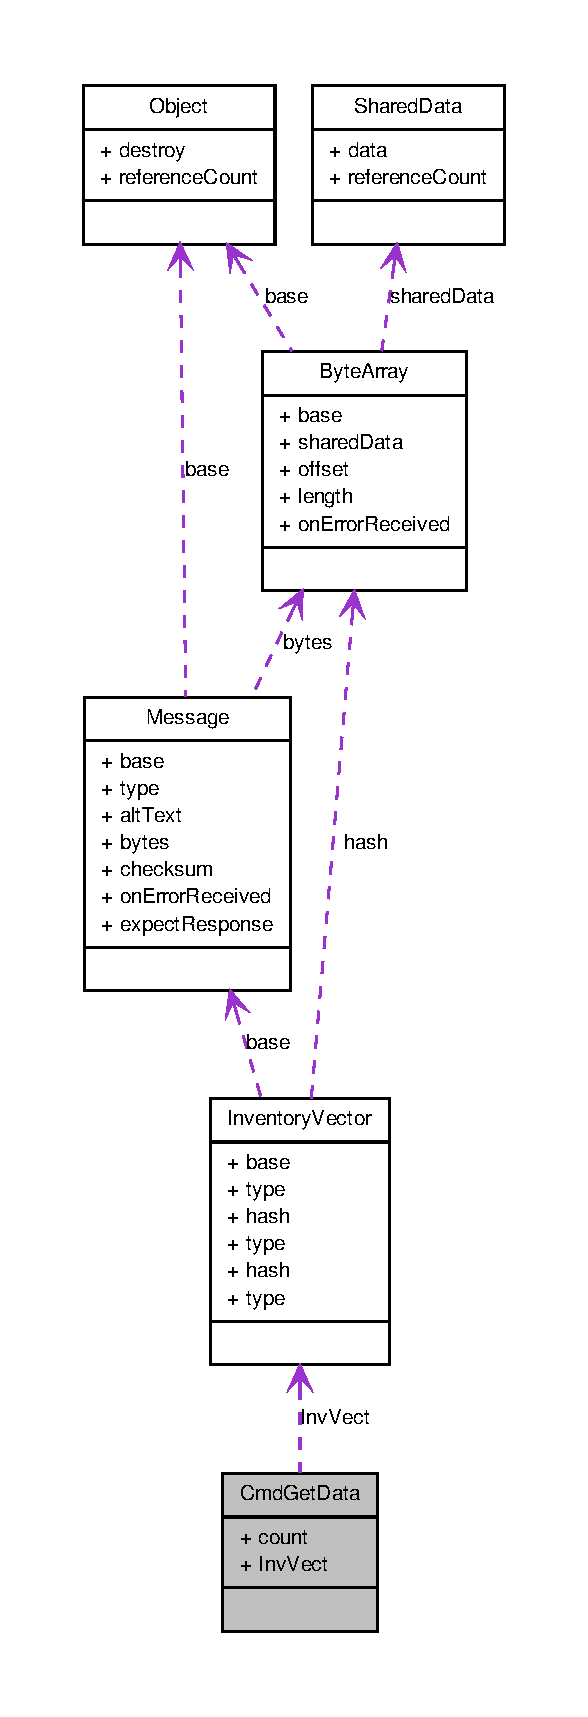
\includegraphics[height=600pt]{struct_cmd_get_data__coll__graph}
\end{center}
\end{figure}
\subsection*{Data Fields}
\begin{DoxyCompactItemize}
\item 
uint64\_\-t \hyperlink{struct_cmd_get_data_afcc68e9eec57ce069fcdc37815837d6d}{count}
\item 
struct \hyperlink{struct_inventory_vector}{InventoryVector} $\ast$ \hyperlink{struct_cmd_get_data_aa0131206f52d276b9c712b34aaff1592}{InvVect}
\end{DoxyCompactItemize}


\subsection{Detailed Description}


Definition at line 119 of file Commands.h.



\subsection{Field Documentation}
\hypertarget{struct_cmd_get_data_afcc68e9eec57ce069fcdc37815837d6d}{
\index{CmdGetData@{CmdGetData}!count@{count}}
\index{count@{count}!CmdGetData@{CmdGetData}}
\subsubsection[{count}]{\setlength{\rightskip}{0pt plus 5cm}uint64\_\-t {\bf count}}}
\label{struct_cmd_get_data_afcc68e9eec57ce069fcdc37815837d6d}


Definition at line 121 of file Commands.h.

\hypertarget{struct_cmd_get_data_aa0131206f52d276b9c712b34aaff1592}{
\index{CmdGetData@{CmdGetData}!InvVect@{InvVect}}
\index{InvVect@{InvVect}!CmdGetData@{CmdGetData}}
\subsubsection[{InvVect}]{\setlength{\rightskip}{0pt plus 5cm}struct {\bf InventoryVector}$\ast$ {\bf InvVect}}}
\label{struct_cmd_get_data_aa0131206f52d276b9c712b34aaff1592}


Definition at line 124 of file Commands.h.



The documentation for this struct was generated from the following file:\begin{DoxyCompactItemize}
\item 
src/Object/NetworkProtocol/\hyperlink{_commands_8h}{Commands.h}\end{DoxyCompactItemize}

\hypertarget{struct_cmd_get_headers}{
\section{CmdGetHeaders Struct Reference}
\label{struct_cmd_get_headers}\index{CmdGetHeaders@{CmdGetHeaders}}
}


{\ttfamily \#include $<$Commands.h$>$}

\subsection*{Data Fields}
\begin{DoxyCompactItemize}
\item 
uint32\_\-t \hyperlink{struct_cmd_get_headers_a3393c33019315a8d7ff4d5e48b0577e8}{startCount}
\item 
char \hyperlink{struct_cmd_get_headers_afb278e99e58307608e33751cd490c97b}{hashStart} \mbox{[}32\mbox{]}
\item 
char \hyperlink{struct_cmd_get_headers_aa16ea670ce42c626f461fc49f74ddcd3}{hashStop} \mbox{[}32\mbox{]}
\end{DoxyCompactItemize}


\subsection{Detailed Description}


Definition at line 136 of file Commands.h.



\subsection{Field Documentation}
\hypertarget{struct_cmd_get_headers_afb278e99e58307608e33751cd490c97b}{
\index{CmdGetHeaders@{CmdGetHeaders}!hashStart@{hashStart}}
\index{hashStart@{hashStart}!CmdGetHeaders@{CmdGetHeaders}}
\subsubsection[{hashStart}]{\setlength{\rightskip}{0pt plus 5cm}char {\bf hashStart}\mbox{[}32\mbox{]}}}
\label{struct_cmd_get_headers_afb278e99e58307608e33751cd490c97b}


Definition at line 138 of file Commands.h.

\hypertarget{struct_cmd_get_headers_aa16ea670ce42c626f461fc49f74ddcd3}{
\index{CmdGetHeaders@{CmdGetHeaders}!hashStop@{hashStop}}
\index{hashStop@{hashStop}!CmdGetHeaders@{CmdGetHeaders}}
\subsubsection[{hashStop}]{\setlength{\rightskip}{0pt plus 5cm}char {\bf hashStop}\mbox{[}32\mbox{]}}}
\label{struct_cmd_get_headers_aa16ea670ce42c626f461fc49f74ddcd3}


Definition at line 139 of file Commands.h.

\hypertarget{struct_cmd_get_headers_a3393c33019315a8d7ff4d5e48b0577e8}{
\index{CmdGetHeaders@{CmdGetHeaders}!startCount@{startCount}}
\index{startCount@{startCount}!CmdGetHeaders@{CmdGetHeaders}}
\subsubsection[{startCount}]{\setlength{\rightskip}{0pt plus 5cm}uint32\_\-t {\bf startCount}}}
\label{struct_cmd_get_headers_a3393c33019315a8d7ff4d5e48b0577e8}


Definition at line 137 of file Commands.h.



The documentation for this struct was generated from the following file:\begin{DoxyCompactItemize}
\item 
src/Object/NetworkProtocol/\hyperlink{_commands_8h}{Commands.h}\end{DoxyCompactItemize}

\hypertarget{struct_cmd_header}{
\section{CmdHeader Struct Reference}
\label{struct_cmd_header}\index{CmdHeader@{CmdHeader}}
}


{\ttfamily \#include $<$Protocol.h$>$}

\subsection*{Data Fields}
\begin{DoxyCompactItemize}
\item 
unsigned int \hyperlink{struct_cmd_header_a7154179fe070a40c828f7c03f454d4d6}{magic}
\item 
char \hyperlink{struct_cmd_header_a5b9e40150e73a908b8815ab282e5a4d3}{command} \mbox{[}12\mbox{]}
\item 
unsigned int \hyperlink{struct_cmd_header_ac8d42bcd4a44e078047ccd7291059238}{length}
\item 
unsigned char \hyperlink{struct_cmd_header_ac1222a6e99fed2d4b20d0713ebf83f34}{CheckSum} \mbox{[}4\mbox{]}
\end{DoxyCompactItemize}


\subsection{Detailed Description}


Definition at line 41 of file Protocol.h.



\subsection{Field Documentation}
\hypertarget{struct_cmd_header_ac1222a6e99fed2d4b20d0713ebf83f34}{
\index{CmdHeader@{CmdHeader}!CheckSum@{CheckSum}}
\index{CheckSum@{CheckSum}!CmdHeader@{CmdHeader}}
\subsubsection[{CheckSum}]{\setlength{\rightskip}{0pt plus 5cm}unsigned char {\bf CheckSum}\mbox{[}4\mbox{]}}}
\label{struct_cmd_header_ac1222a6e99fed2d4b20d0713ebf83f34}


Definition at line 45 of file Protocol.h.

\hypertarget{struct_cmd_header_a5b9e40150e73a908b8815ab282e5a4d3}{
\index{CmdHeader@{CmdHeader}!command@{command}}
\index{command@{command}!CmdHeader@{CmdHeader}}
\subsubsection[{command}]{\setlength{\rightskip}{0pt plus 5cm}char {\bf command}\mbox{[}12\mbox{]}}}
\label{struct_cmd_header_a5b9e40150e73a908b8815ab282e5a4d3}


Definition at line 43 of file Protocol.h.

\hypertarget{struct_cmd_header_ac8d42bcd4a44e078047ccd7291059238}{
\index{CmdHeader@{CmdHeader}!length@{length}}
\index{length@{length}!CmdHeader@{CmdHeader}}
\subsubsection[{length}]{\setlength{\rightskip}{0pt plus 5cm}unsigned int {\bf length}}}
\label{struct_cmd_header_ac8d42bcd4a44e078047ccd7291059238}


Definition at line 44 of file Protocol.h.

\hypertarget{struct_cmd_header_a7154179fe070a40c828f7c03f454d4d6}{
\index{CmdHeader@{CmdHeader}!magic@{magic}}
\index{magic@{magic}!CmdHeader@{CmdHeader}}
\subsubsection[{magic}]{\setlength{\rightskip}{0pt plus 5cm}unsigned int {\bf magic}}}
\label{struct_cmd_header_a7154179fe070a40c828f7c03f454d4d6}


Definition at line 42 of file Protocol.h.



The documentation for this struct was generated from the following file:\begin{DoxyCompactItemize}
\item 
src/Object/NetworkProtocol/\hyperlink{_protocol_8h}{Protocol.h}\end{DoxyCompactItemize}

\hypertarget{struct_cmd_header_check_sum}{
\section{CmdHeaderCheckSum Struct Reference}
\label{struct_cmd_header_check_sum}\index{CmdHeaderCheckSum@{CmdHeaderCheckSum}}
}


{\ttfamily \#include $<$Protocol.h$>$}

\subsection*{Data Fields}
\begin{DoxyCompactItemize}
\item 
unsigned int \hyperlink{struct_cmd_header_check_sum_a7154179fe070a40c828f7c03f454d4d6}{magic}
\item 
char \hyperlink{struct_cmd_header_check_sum_a5b9e40150e73a908b8815ab282e5a4d3}{command} \mbox{[}12\mbox{]}
\item 
unsigned int \hyperlink{struct_cmd_header_check_sum_ac8d42bcd4a44e078047ccd7291059238}{length}
\end{DoxyCompactItemize}


\subsection{Detailed Description}


Definition at line 50 of file Protocol.h.



\subsection{Field Documentation}
\hypertarget{struct_cmd_header_check_sum_a5b9e40150e73a908b8815ab282e5a4d3}{
\index{CmdHeaderCheckSum@{CmdHeaderCheckSum}!command@{command}}
\index{command@{command}!CmdHeaderCheckSum@{CmdHeaderCheckSum}}
\subsubsection[{command}]{\setlength{\rightskip}{0pt plus 5cm}char {\bf command}\mbox{[}12\mbox{]}}}
\label{struct_cmd_header_check_sum_a5b9e40150e73a908b8815ab282e5a4d3}


Definition at line 52 of file Protocol.h.

\hypertarget{struct_cmd_header_check_sum_ac8d42bcd4a44e078047ccd7291059238}{
\index{CmdHeaderCheckSum@{CmdHeaderCheckSum}!length@{length}}
\index{length@{length}!CmdHeaderCheckSum@{CmdHeaderCheckSum}}
\subsubsection[{length}]{\setlength{\rightskip}{0pt plus 5cm}unsigned int {\bf length}}}
\label{struct_cmd_header_check_sum_ac8d42bcd4a44e078047ccd7291059238}


Definition at line 53 of file Protocol.h.

\hypertarget{struct_cmd_header_check_sum_a7154179fe070a40c828f7c03f454d4d6}{
\index{CmdHeaderCheckSum@{CmdHeaderCheckSum}!magic@{magic}}
\index{magic@{magic}!CmdHeaderCheckSum@{CmdHeaderCheckSum}}
\subsubsection[{magic}]{\setlength{\rightskip}{0pt plus 5cm}unsigned int {\bf magic}}}
\label{struct_cmd_header_check_sum_a7154179fe070a40c828f7c03f454d4d6}


Definition at line 51 of file Protocol.h.



The documentation for this struct was generated from the following file:\begin{DoxyCompactItemize}
\item 
src/Object/NetworkProtocol/\hyperlink{_protocol_8h}{Protocol.h}\end{DoxyCompactItemize}

\hypertarget{struct_cmd_headers}{
\section{CmdHeaders Struct Reference}
\label{struct_cmd_headers}\index{CmdHeaders@{CmdHeaders}}
}


{\ttfamily \#include $<$Commands.h$>$}



\subsection{Detailed Description}


Definition at line 164 of file Commands.h.



The documentation for this struct was generated from the following file:\begin{DoxyCompactItemize}
\item 
src/Object/NetworkProtocol/\hyperlink{_commands_8h}{Commands.h}\end{DoxyCompactItemize}

\hypertarget{struct_cmd_inv}{
\section{CmdInv Struct Reference}
\label{struct_cmd_inv}\index{CmdInv@{CmdInv}}
}


{\ttfamily \#include $<$Commands.h$>$}



Collaboration diagram for CmdInv:
\nopagebreak
\begin{figure}[H]
\begin{center}
\leavevmode
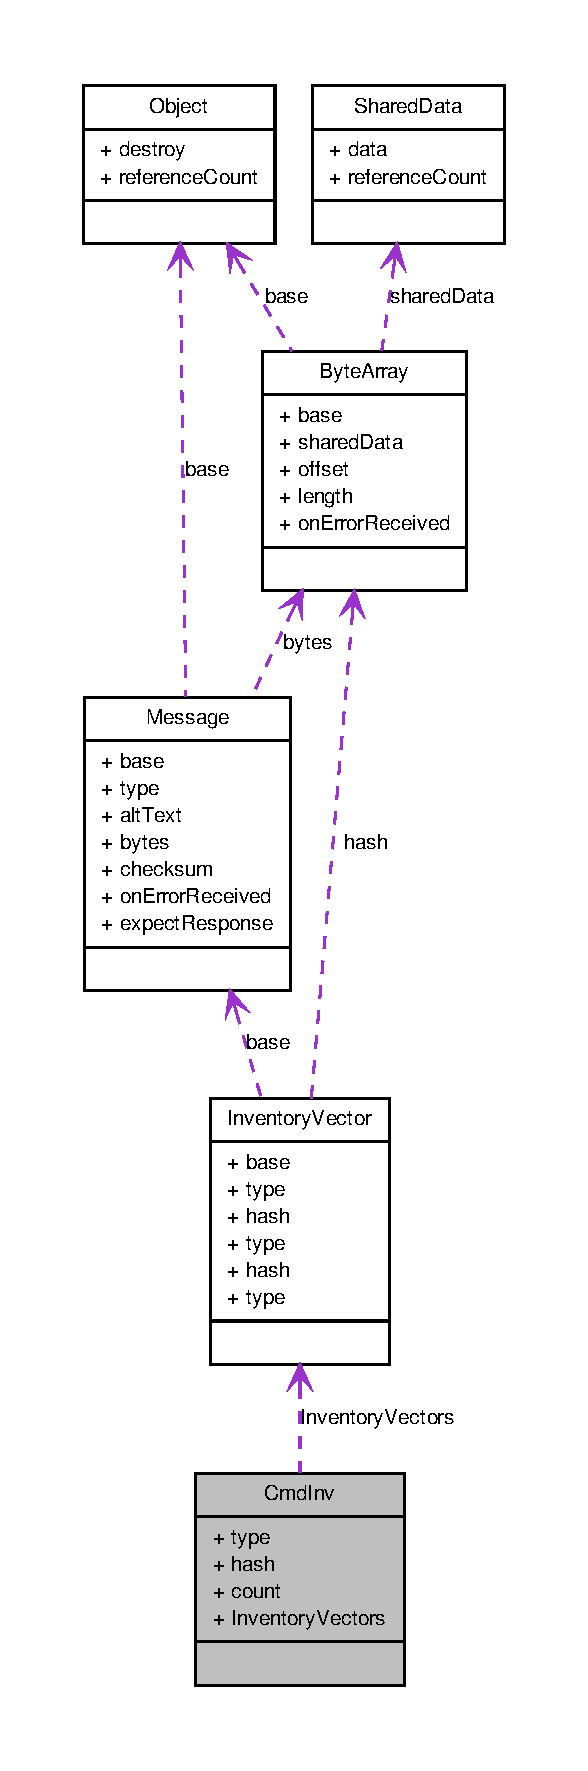
\includegraphics[height=600pt]{struct_cmd_inv__coll__graph}
\end{center}
\end{figure}
\subsection*{Data Fields}
\begin{DoxyCompactItemize}
\item 
uint32\_\-t \hyperlink{struct_cmd_inv_ad44b615021ed3ccb734fcaf583ef4a03}{type}
\item 
char \hyperlink{struct_cmd_inv_a30660ee1bca7189182e64c5a192651af}{hash} \mbox{[}32\mbox{]}
\item 
unsigned int \hyperlink{struct_cmd_inv_a16ff2d8e15ade4948398b0aeb80124a8}{count}
\item 
struct \hyperlink{struct_inventory_vector}{InventoryVector} $\ast$ \hyperlink{struct_cmd_inv_ab98754c1df21fac25844fc908ecefe29}{InventoryVectors}
\end{DoxyCompactItemize}


\subsection{Detailed Description}


Definition at line 112 of file Commands.h.



\subsection{Field Documentation}
\hypertarget{struct_cmd_inv_a16ff2d8e15ade4948398b0aeb80124a8}{
\index{CmdInv@{CmdInv}!count@{count}}
\index{count@{count}!CmdInv@{CmdInv}}
\subsubsection[{count}]{\setlength{\rightskip}{0pt plus 5cm}unsigned int {\bf count}}}
\label{struct_cmd_inv_a16ff2d8e15ade4948398b0aeb80124a8}


Definition at line 121 of file Protocol.h.

\hypertarget{struct_cmd_inv_a30660ee1bca7189182e64c5a192651af}{
\index{CmdInv@{CmdInv}!hash@{hash}}
\index{hash@{hash}!CmdInv@{CmdInv}}
\subsubsection[{hash}]{\setlength{\rightskip}{0pt plus 5cm}char {\bf hash}\mbox{[}32\mbox{]}}}
\label{struct_cmd_inv_a30660ee1bca7189182e64c5a192651af}


Definition at line 116 of file Commands.h.

\hypertarget{struct_cmd_inv_ab98754c1df21fac25844fc908ecefe29}{
\index{CmdInv@{CmdInv}!InventoryVectors@{InventoryVectors}}
\index{InventoryVectors@{InventoryVectors}!CmdInv@{CmdInv}}
\subsubsection[{InventoryVectors}]{\setlength{\rightskip}{0pt plus 5cm}struct {\bf InventoryVector}$\ast$ {\bf InventoryVectors}}}
\label{struct_cmd_inv_ab98754c1df21fac25844fc908ecefe29}


Definition at line 122 of file Protocol.h.

\hypertarget{struct_cmd_inv_ad44b615021ed3ccb734fcaf583ef4a03}{
\index{CmdInv@{CmdInv}!type@{type}}
\index{type@{type}!CmdInv@{CmdInv}}
\subsubsection[{type}]{\setlength{\rightskip}{0pt plus 5cm}uint32\_\-t {\bf type}}}
\label{struct_cmd_inv_ad44b615021ed3ccb734fcaf583ef4a03}


Definition at line 114 of file Commands.h.



The documentation for this struct was generated from the following files:\begin{DoxyCompactItemize}
\item 
src/Object/NetworkProtocol/\hyperlink{_commands_8h}{Commands.h}\item 
src/Object/NetworkProtocol/\hyperlink{_protocol_8h}{Protocol.h}\end{DoxyCompactItemize}

\hypertarget{struct_cmd_ping}{
\section{CmdPing Struct Reference}
\label{struct_cmd_ping}\index{CmdPing@{CmdPing}}
}


{\ttfamily \#include $<$Commands.h$>$}



\subsection{Detailed Description}


Definition at line 184 of file Commands.h.



The documentation for this struct was generated from the following file:\begin{DoxyCompactItemize}
\item 
src/Object/NetworkProtocol/\hyperlink{_commands_8h}{Commands.h}\end{DoxyCompactItemize}

\hypertarget{struct_cmd_reply}{
\section{CmdReply Struct Reference}
\label{struct_cmd_reply}\index{CmdReply@{CmdReply}}
}


{\ttfamily \#include $<$Commands.h$>$}



\subsection{Detailed Description}


Definition at line 180 of file Commands.h.



The documentation for this struct was generated from the following file:\begin{DoxyCompactItemize}
\item 
src/Object/NetworkProtocol/\hyperlink{_commands_8h}{Commands.h}\end{DoxyCompactItemize}

\hypertarget{struct_cmd_submit_order}{
\section{CmdSubmitOrder Struct Reference}
\label{struct_cmd_submit_order}\index{CmdSubmitOrder@{CmdSubmitOrder}}
}


{\ttfamily \#include $<$Commands.h$>$}



\subsection{Detailed Description}


Definition at line 176 of file Commands.h.



The documentation for this struct was generated from the following file:\begin{DoxyCompactItemize}
\item 
src/Object/NetworkProtocol/\hyperlink{_commands_8h}{Commands.h}\end{DoxyCompactItemize}

\hypertarget{struct_cmd_tranx}{
\section{CmdTranx Struct Reference}
\label{struct_cmd_tranx}\index{CmdTranx@{CmdTranx}}
}


{\ttfamily \#include $<$Commands.h$>$}



Collaboration diagram for CmdTranx:\nopagebreak
\begin{figure}[H]
\begin{center}
\leavevmode
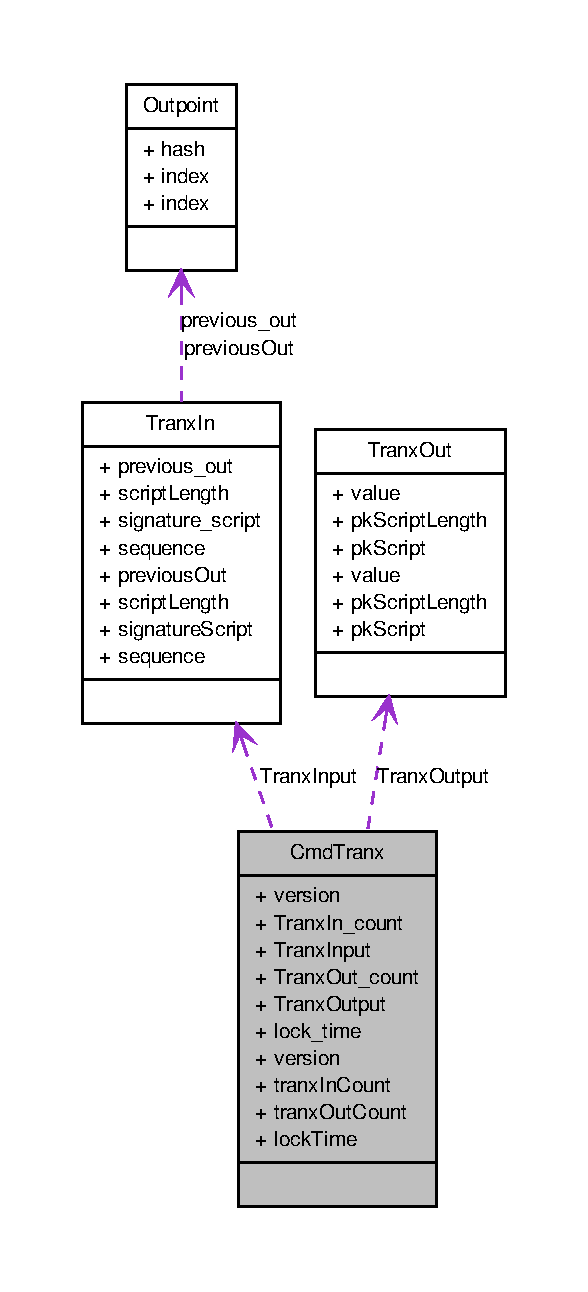
\includegraphics[height=600pt]{struct_cmd_tranx__coll__graph}
\end{center}
\end{figure}
\subsection*{Data Fields}
\begin{DoxyCompactItemize}
\item 
uint32\_\-t \hyperlink{struct_cmd_tranx_acd99bb05ca015e7d74448acb1deba7ca}{version}
\item 
uint32\_\-t \hyperlink{struct_cmd_tranx_a29cd42e9db0010d7b5bb283bf2604765}{TranxIn\_\-count}
\item 
struct \hyperlink{struct_tranx_in}{TranxIn} $\ast$ \hyperlink{struct_cmd_tranx_a5b66f083197ffa9abe32484db40fcd39}{TranxInput}
\item 
uint32\_\-t \hyperlink{struct_cmd_tranx_a64038348b38f758be9417994e2f823a3}{TranxOut\_\-count}
\item 
struct \hyperlink{struct_tranx_out}{TranxOut} $\ast$ \hyperlink{struct_cmd_tranx_afd763f710fae1f1cefe4c6260c1a5568}{TranxOutput}
\item 
uint32\_\-t \hyperlink{struct_cmd_tranx_a54e5a5f03919a5838067d81ddc5efda4}{lock\_\-time}
\item 
unsigned int \hyperlink{struct_cmd_tranx_a5408ac5df4c170828874e1b10b4c35a0}{version}
\item 
unsigned int \hyperlink{struct_cmd_tranx_aee4a92ad1604309b8526009831b57c58}{tranxInCount}
\item 
unsigned int \hyperlink{struct_cmd_tranx_a6508946c345b4ea761a9d66c38a5fe7a}{tranxOutCount}
\item 
unsigned int \hyperlink{struct_cmd_tranx_ace6436ac55ff63b037da554bf1ddfc32}{lockTime}
\end{DoxyCompactItemize}


\subsection{Detailed Description}


Definition at line 142 of file Commands.h.



\subsection{Field Documentation}
\hypertarget{struct_cmd_tranx_a54e5a5f03919a5838067d81ddc5efda4}{
\index{CmdTranx@{CmdTranx}!lock\_\-time@{lock\_\-time}}
\index{lock\_\-time@{lock\_\-time}!CmdTranx@{CmdTranx}}
\subsubsection[{lock\_\-time}]{\setlength{\rightskip}{0pt plus 5cm}uint32\_\-t {\bf lock\_\-time}}}
\label{struct_cmd_tranx_a54e5a5f03919a5838067d81ddc5efda4}


Definition at line 148 of file Commands.h.

\hypertarget{struct_cmd_tranx_ace6436ac55ff63b037da554bf1ddfc32}{
\index{CmdTranx@{CmdTranx}!lockTime@{lockTime}}
\index{lockTime@{lockTime}!CmdTranx@{CmdTranx}}
\subsubsection[{lockTime}]{\setlength{\rightskip}{0pt plus 5cm}unsigned int {\bf lockTime}}}
\label{struct_cmd_tranx_ace6436ac55ff63b037da554bf1ddfc32}


Definition at line 178 of file Protocol.h.

\hypertarget{struct_cmd_tranx_a29cd42e9db0010d7b5bb283bf2604765}{
\index{CmdTranx@{CmdTranx}!TranxIn\_\-count@{TranxIn\_\-count}}
\index{TranxIn\_\-count@{TranxIn\_\-count}!CmdTranx@{CmdTranx}}
\subsubsection[{TranxIn\_\-count}]{\setlength{\rightskip}{0pt plus 5cm}uint32\_\-t {\bf TranxIn\_\-count}}}
\label{struct_cmd_tranx_a29cd42e9db0010d7b5bb283bf2604765}


Definition at line 144 of file Commands.h.

\hypertarget{struct_cmd_tranx_aee4a92ad1604309b8526009831b57c58}{
\index{CmdTranx@{CmdTranx}!tranxInCount@{tranxInCount}}
\index{tranxInCount@{tranxInCount}!CmdTranx@{CmdTranx}}
\subsubsection[{tranxInCount}]{\setlength{\rightskip}{0pt plus 5cm}unsigned int {\bf tranxInCount}}}
\label{struct_cmd_tranx_aee4a92ad1604309b8526009831b57c58}


Definition at line 174 of file Protocol.h.

\hypertarget{struct_cmd_tranx_a5b66f083197ffa9abe32484db40fcd39}{
\index{CmdTranx@{CmdTranx}!TranxInput@{TranxInput}}
\index{TranxInput@{TranxInput}!CmdTranx@{CmdTranx}}
\subsubsection[{TranxInput}]{\setlength{\rightskip}{0pt plus 5cm}struct {\bf TranxIn} $\ast$ {\bf TranxInput}}}
\label{struct_cmd_tranx_a5b66f083197ffa9abe32484db40fcd39}


Definition at line 145 of file Commands.h.

\hypertarget{struct_cmd_tranx_a64038348b38f758be9417994e2f823a3}{
\index{CmdTranx@{CmdTranx}!TranxOut\_\-count@{TranxOut\_\-count}}
\index{TranxOut\_\-count@{TranxOut\_\-count}!CmdTranx@{CmdTranx}}
\subsubsection[{TranxOut\_\-count}]{\setlength{\rightskip}{0pt plus 5cm}uint32\_\-t {\bf TranxOut\_\-count}}}
\label{struct_cmd_tranx_a64038348b38f758be9417994e2f823a3}


Definition at line 146 of file Commands.h.

\hypertarget{struct_cmd_tranx_a6508946c345b4ea761a9d66c38a5fe7a}{
\index{CmdTranx@{CmdTranx}!tranxOutCount@{tranxOutCount}}
\index{tranxOutCount@{tranxOutCount}!CmdTranx@{CmdTranx}}
\subsubsection[{tranxOutCount}]{\setlength{\rightskip}{0pt plus 5cm}unsigned int {\bf tranxOutCount}}}
\label{struct_cmd_tranx_a6508946c345b4ea761a9d66c38a5fe7a}


Definition at line 176 of file Protocol.h.

\hypertarget{struct_cmd_tranx_afd763f710fae1f1cefe4c6260c1a5568}{
\index{CmdTranx@{CmdTranx}!TranxOutput@{TranxOutput}}
\index{TranxOutput@{TranxOutput}!CmdTranx@{CmdTranx}}
\subsubsection[{TranxOutput}]{\setlength{\rightskip}{0pt plus 5cm}struct {\bf TranxOut} $\ast$ {\bf TranxOutput}}}
\label{struct_cmd_tranx_afd763f710fae1f1cefe4c6260c1a5568}


Definition at line 147 of file Commands.h.

\hypertarget{struct_cmd_tranx_a5408ac5df4c170828874e1b10b4c35a0}{
\index{CmdTranx@{CmdTranx}!version@{version}}
\index{version@{version}!CmdTranx@{CmdTranx}}
\subsubsection[{version}]{\setlength{\rightskip}{0pt plus 5cm}unsigned int {\bf version}}}
\label{struct_cmd_tranx_a5408ac5df4c170828874e1b10b4c35a0}


Definition at line 173 of file Protocol.h.

\hypertarget{struct_cmd_tranx_acd99bb05ca015e7d74448acb1deba7ca}{
\index{CmdTranx@{CmdTranx}!version@{version}}
\index{version@{version}!CmdTranx@{CmdTranx}}
\subsubsection[{version}]{\setlength{\rightskip}{0pt plus 5cm}uint32\_\-t {\bf version}}}
\label{struct_cmd_tranx_acd99bb05ca015e7d74448acb1deba7ca}


Definition at line 143 of file Commands.h.



The documentation for this struct was generated from the following files:\begin{DoxyCompactItemize}
\item 
src/Object/NetworkProtocol/\hyperlink{_commands_8h}{Commands.h}\item 
src/Object/NetworkProtocol/\hyperlink{_protocol_8h}{Protocol.h}\end{DoxyCompactItemize}

\hypertarget{struct_cmd_verack}{
\section{CmdVerack Struct Reference}
\label{struct_cmd_verack}\index{CmdVerack@{CmdVerack}}
}


{\ttfamily \#include $<$Commands.h$>$}

\subsection*{Data Fields}
\begin{DoxyCompactItemize}
\item 
uint32\_\-t \hyperlink{struct_cmd_verack_a57f54349f4fd1cbbb52058812e146af2}{magic}
\item 
char \hyperlink{struct_cmd_verack_a5b9e40150e73a908b8815ab282e5a4d3}{command} \mbox{[}12\mbox{]}
\item 
uint32\_\-t \hyperlink{struct_cmd_verack_aebb70c2aab3407a9f05334c47131a43b}{length}
\item 
uint32\_\-t \hyperlink{struct_cmd_verack_aa482bc33779a87f57ab8efc2c1680c48}{checksum}
\item 
unsigned char $\ast$ \hyperlink{struct_cmd_verack_a330f1bb25881c43b17265cdc48d8b5a2}{payload}
\end{DoxyCompactItemize}


\subsection{Detailed Description}


Definition at line 90 of file Commands.h.



\subsection{Field Documentation}
\hypertarget{struct_cmd_verack_aa482bc33779a87f57ab8efc2c1680c48}{
\index{CmdVerack@{CmdVerack}!checksum@{checksum}}
\index{checksum@{checksum}!CmdVerack@{CmdVerack}}
\subsubsection[{checksum}]{\setlength{\rightskip}{0pt plus 5cm}uint32\_\-t {\bf checksum}}}
\label{struct_cmd_verack_aa482bc33779a87f57ab8efc2c1680c48}


Definition at line 97 of file Commands.h.

\hypertarget{struct_cmd_verack_a5b9e40150e73a908b8815ab282e5a4d3}{
\index{CmdVerack@{CmdVerack}!command@{command}}
\index{command@{command}!CmdVerack@{CmdVerack}}
\subsubsection[{command}]{\setlength{\rightskip}{0pt plus 5cm}char {\bf command}\mbox{[}12\mbox{]}}}
\label{struct_cmd_verack_a5b9e40150e73a908b8815ab282e5a4d3}


Definition at line 95 of file Commands.h.

\hypertarget{struct_cmd_verack_aebb70c2aab3407a9f05334c47131a43b}{
\index{CmdVerack@{CmdVerack}!length@{length}}
\index{length@{length}!CmdVerack@{CmdVerack}}
\subsubsection[{length}]{\setlength{\rightskip}{0pt plus 5cm}uint32\_\-t {\bf length}}}
\label{struct_cmd_verack_aebb70c2aab3407a9f05334c47131a43b}


Definition at line 96 of file Commands.h.

\hypertarget{struct_cmd_verack_a57f54349f4fd1cbbb52058812e146af2}{
\index{CmdVerack@{CmdVerack}!magic@{magic}}
\index{magic@{magic}!CmdVerack@{CmdVerack}}
\subsubsection[{magic}]{\setlength{\rightskip}{0pt plus 5cm}uint32\_\-t {\bf magic}}}
\label{struct_cmd_verack_a57f54349f4fd1cbbb52058812e146af2}


Definition at line 92 of file Commands.h.

\hypertarget{struct_cmd_verack_a330f1bb25881c43b17265cdc48d8b5a2}{
\index{CmdVerack@{CmdVerack}!payload@{payload}}
\index{payload@{payload}!CmdVerack@{CmdVerack}}
\subsubsection[{payload}]{\setlength{\rightskip}{0pt plus 5cm}unsigned char$\ast$ {\bf payload}}}
\label{struct_cmd_verack_a330f1bb25881c43b17265cdc48d8b5a2}


Definition at line 98 of file Commands.h.



The documentation for this struct was generated from the following file:\begin{DoxyCompactItemize}
\item 
src/Object/NetworkProtocol/\hyperlink{_commands_8h}{Commands.h}\end{DoxyCompactItemize}

\hypertarget{struct_cmd_version}{
\section{CmdVersion Struct Reference}
\label{struct_cmd_version}\index{CmdVersion@{CmdVersion}}
}


{\ttfamily \#include $<$Commands.h$>$}



Collaboration diagram for CmdVersion:\nopagebreak
\begin{figure}[H]
\begin{center}
\leavevmode
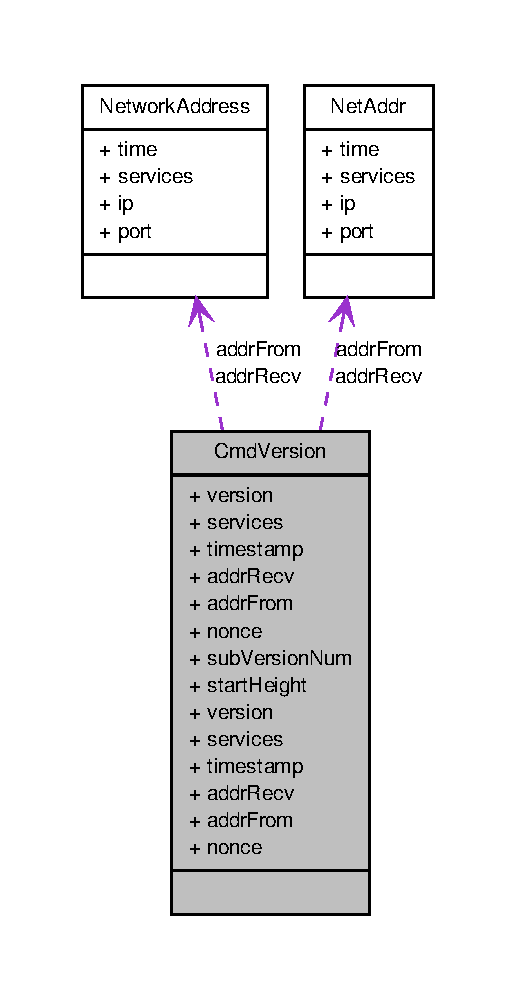
\includegraphics[width=248pt]{struct_cmd_version__coll__graph}
\end{center}
\end{figure}
\subsection*{Data Fields}
\begin{DoxyCompactItemize}
\item 
int32\_\-t \hyperlink{struct_cmd_version_a67fae7dd1de9edce3656ed214d20377f}{version}
\item 
uint64\_\-t \hyperlink{struct_cmd_version_a8361260b2ca75771b8da0333191db456}{services}
\item 
int64\_\-t \hyperlink{struct_cmd_version_a8a591d341723df9496cda98e225b25b4}{timestamp}
\item 
struct \hyperlink{struct_network_address}{NetworkAddress} \hyperlink{struct_cmd_version_a1c343f8763f536140c776a99d43ecde3}{addrRecv}
\item 
struct \hyperlink{struct_network_address}{NetworkAddress} \hyperlink{struct_cmd_version_a459e4f223be92dc8d26e577d85ba4334}{addrFrom}
\item 
uint64\_\-t \hyperlink{struct_cmd_version_af602af589d5bc1af695356386bcb32a9}{nonce}
\item 
char $\ast$ \hyperlink{struct_cmd_version_abe98c3c041a6acda8de5e4052aff3ccd}{subVersionNum}
\item 
int32\_\-t \hyperlink{struct_cmd_version_a75434fa1cfbff59d821bd10ba0cb6df1}{startHeight}
\item 
unsigned int \hyperlink{struct_cmd_version_a5408ac5df4c170828874e1b10b4c35a0}{version}
\item 
long int \hyperlink{struct_cmd_version_a7c2c2697560cb0d08fdca3bd4d10d07e}{services}
\item 
long int \hyperlink{struct_cmd_version_ac402a8520447a72d85baad30fb7d66af}{timestamp}
\item 
struct \hyperlink{struct_net_addr}{NetAddr} \hyperlink{struct_cmd_version_a252b04dc9767f81b38eccddcd72e74ff}{addrRecv}
\item 
struct \hyperlink{struct_net_addr}{NetAddr} \hyperlink{struct_cmd_version_acbbb94e30bbe4e7c99be8e4c61f1e79c}{addrFrom}
\item 
long int \hyperlink{struct_cmd_version_ab0c4e6e9b4c0db0818ba6121afe137a9}{nonce}
\end{DoxyCompactItemize}


\subsection{Detailed Description}


Definition at line 55 of file Commands.h.



\subsection{Field Documentation}
\hypertarget{struct_cmd_version_a459e4f223be92dc8d26e577d85ba4334}{
\index{CmdVersion@{CmdVersion}!addrFrom@{addrFrom}}
\index{addrFrom@{addrFrom}!CmdVersion@{CmdVersion}}
\subsubsection[{addrFrom}]{\setlength{\rightskip}{0pt plus 5cm}struct {\bf NetworkAddress} {\bf addrFrom}}}
\label{struct_cmd_version_a459e4f223be92dc8d26e577d85ba4334}


Definition at line 73 of file Commands.h.

\hypertarget{struct_cmd_version_acbbb94e30bbe4e7c99be8e4c61f1e79c}{
\index{CmdVersion@{CmdVersion}!addrFrom@{addrFrom}}
\index{addrFrom@{addrFrom}!CmdVersion@{CmdVersion}}
\subsubsection[{addrFrom}]{\setlength{\rightskip}{0pt plus 5cm}struct {\bf NetAddr} {\bf addrFrom}}}
\label{struct_cmd_version_acbbb94e30bbe4e7c99be8e4c61f1e79c}


Definition at line 76 of file Protocol.h.

\hypertarget{struct_cmd_version_a1c343f8763f536140c776a99d43ecde3}{
\index{CmdVersion@{CmdVersion}!addrRecv@{addrRecv}}
\index{addrRecv@{addrRecv}!CmdVersion@{CmdVersion}}
\subsubsection[{addrRecv}]{\setlength{\rightskip}{0pt plus 5cm}struct {\bf NetworkAddress} {\bf addrRecv}}}
\label{struct_cmd_version_a1c343f8763f536140c776a99d43ecde3}


Definition at line 68 of file Commands.h.

\hypertarget{struct_cmd_version_a252b04dc9767f81b38eccddcd72e74ff}{
\index{CmdVersion@{CmdVersion}!addrRecv@{addrRecv}}
\index{addrRecv@{addrRecv}!CmdVersion@{CmdVersion}}
\subsubsection[{addrRecv}]{\setlength{\rightskip}{0pt plus 5cm}struct {\bf NetAddr} {\bf addrRecv}}}
\label{struct_cmd_version_a252b04dc9767f81b38eccddcd72e74ff}


Definition at line 73 of file Protocol.h.

\hypertarget{struct_cmd_version_af602af589d5bc1af695356386bcb32a9}{
\index{CmdVersion@{CmdVersion}!nonce@{nonce}}
\index{nonce@{nonce}!CmdVersion@{CmdVersion}}
\subsubsection[{nonce}]{\setlength{\rightskip}{0pt plus 5cm}uint64\_\-t {\bf nonce}}}
\label{struct_cmd_version_af602af589d5bc1af695356386bcb32a9}


Definition at line 79 of file Commands.h.

\hypertarget{struct_cmd_version_ab0c4e6e9b4c0db0818ba6121afe137a9}{
\index{CmdVersion@{CmdVersion}!nonce@{nonce}}
\index{nonce@{nonce}!CmdVersion@{CmdVersion}}
\subsubsection[{nonce}]{\setlength{\rightskip}{0pt plus 5cm}long int {\bf nonce}}}
\label{struct_cmd_version_ab0c4e6e9b4c0db0818ba6121afe137a9}


Definition at line 77 of file Protocol.h.

\hypertarget{struct_cmd_version_a8361260b2ca75771b8da0333191db456}{
\index{CmdVersion@{CmdVersion}!services@{services}}
\index{services@{services}!CmdVersion@{CmdVersion}}
\subsubsection[{services}]{\setlength{\rightskip}{0pt plus 5cm}uint64\_\-t {\bf services}}}
\label{struct_cmd_version_a8361260b2ca75771b8da0333191db456}


Definition at line 62 of file Commands.h.

\hypertarget{struct_cmd_version_a7c2c2697560cb0d08fdca3bd4d10d07e}{
\index{CmdVersion@{CmdVersion}!services@{services}}
\index{services@{services}!CmdVersion@{CmdVersion}}
\subsubsection[{services}]{\setlength{\rightskip}{0pt plus 5cm}long int {\bf services}}}
\label{struct_cmd_version_a7c2c2697560cb0d08fdca3bd4d10d07e}


Definition at line 71 of file Protocol.h.

\hypertarget{struct_cmd_version_a75434fa1cfbff59d821bd10ba0cb6df1}{
\index{CmdVersion@{CmdVersion}!startHeight@{startHeight}}
\index{startHeight@{startHeight}!CmdVersion@{CmdVersion}}
\subsubsection[{startHeight}]{\setlength{\rightskip}{0pt plus 5cm}int32\_\-t {\bf startHeight}}}
\label{struct_cmd_version_a75434fa1cfbff59d821bd10ba0cb6df1}


Definition at line 87 of file Commands.h.

\hypertarget{struct_cmd_version_abe98c3c041a6acda8de5e4052aff3ccd}{
\index{CmdVersion@{CmdVersion}!subVersionNum@{subVersionNum}}
\index{subVersionNum@{subVersionNum}!CmdVersion@{CmdVersion}}
\subsubsection[{subVersionNum}]{\setlength{\rightskip}{0pt plus 5cm}char$\ast$ {\bf subVersionNum}}}
\label{struct_cmd_version_abe98c3c041a6acda8de5e4052aff3ccd}


Definition at line 82 of file Commands.h.

\hypertarget{struct_cmd_version_ac402a8520447a72d85baad30fb7d66af}{
\index{CmdVersion@{CmdVersion}!timestamp@{timestamp}}
\index{timestamp@{timestamp}!CmdVersion@{CmdVersion}}
\subsubsection[{timestamp}]{\setlength{\rightskip}{0pt plus 5cm}long int {\bf timestamp}}}
\label{struct_cmd_version_ac402a8520447a72d85baad30fb7d66af}


Definition at line 72 of file Protocol.h.

\hypertarget{struct_cmd_version_a8a591d341723df9496cda98e225b25b4}{
\index{CmdVersion@{CmdVersion}!timestamp@{timestamp}}
\index{timestamp@{timestamp}!CmdVersion@{CmdVersion}}
\subsubsection[{timestamp}]{\setlength{\rightskip}{0pt plus 5cm}int64\_\-t {\bf timestamp}}}
\label{struct_cmd_version_a8a591d341723df9496cda98e225b25b4}


Definition at line 65 of file Commands.h.

\hypertarget{struct_cmd_version_a67fae7dd1de9edce3656ed214d20377f}{
\index{CmdVersion@{CmdVersion}!version@{version}}
\index{version@{version}!CmdVersion@{CmdVersion}}
\subsubsection[{version}]{\setlength{\rightskip}{0pt plus 5cm}int32\_\-t {\bf version}}}
\label{struct_cmd_version_a67fae7dd1de9edce3656ed214d20377f}


Definition at line 59 of file Commands.h.

\hypertarget{struct_cmd_version_a5408ac5df4c170828874e1b10b4c35a0}{
\index{CmdVersion@{CmdVersion}!version@{version}}
\index{version@{version}!CmdVersion@{CmdVersion}}
\subsubsection[{version}]{\setlength{\rightskip}{0pt plus 5cm}unsigned int {\bf version}}}
\label{struct_cmd_version_a5408ac5df4c170828874e1b10b4c35a0}


Definition at line 70 of file Protocol.h.



The documentation for this struct was generated from the following files:\begin{DoxyCompactItemize}
\item 
src/Object/NetworkProtocol/\hyperlink{_commands_8h}{Commands.h}\item 
src/Object/NetworkProtocol/\hyperlink{_protocol_8h}{Protocol.h}\end{DoxyCompactItemize}

\hypertarget{struct_get_blocks}{
\section{GetBlocks Struct Reference}
\label{struct_get_blocks}\index{GetBlocks@{GetBlocks}}
}


Structure for \hyperlink{struct_get_blocks}{GetBlocks} objects.  




{\ttfamily \#include $<$GetBlocks.h$>$}



Collaboration diagram for GetBlocks:
\nopagebreak
\begin{figure}[H]
\begin{center}
\leavevmode
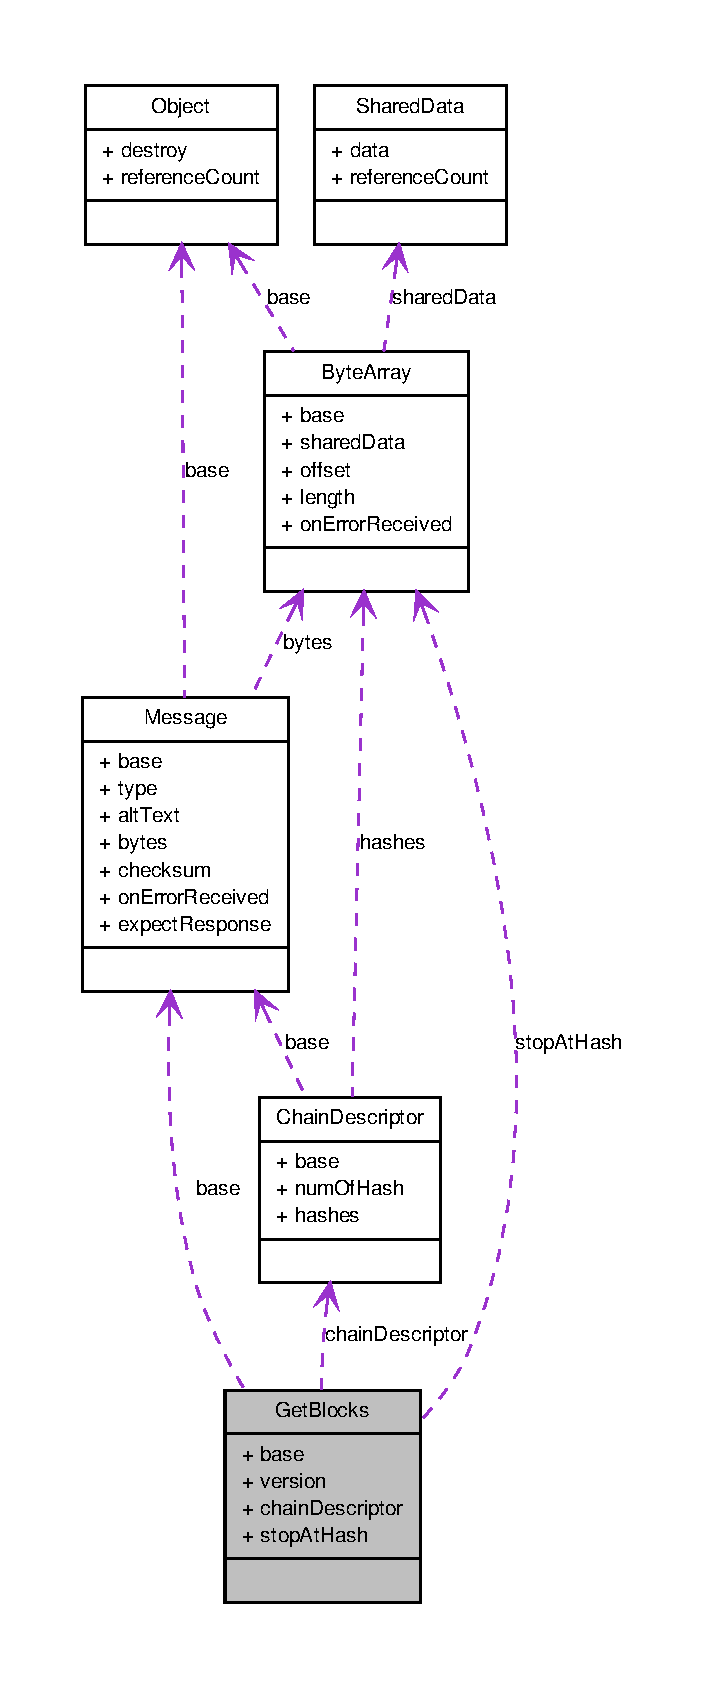
\includegraphics[height=600pt]{struct_get_blocks__coll__graph}
\end{center}
\end{figure}
\subsection*{Data Fields}
\begin{DoxyCompactItemize}
\item 
\hyperlink{struct_message}{Message} \hyperlink{struct_get_blocks_a8987f797adf70c3e174fd64cc68bc933}{base}
\item 
uint32\_\-t \hyperlink{struct_get_blocks_acd99bb05ca015e7d74448acb1deba7ca}{version}
\item 
\hyperlink{struct_chain_descriptor}{ChainDescriptor} $\ast$ \hyperlink{struct_get_blocks_a97f23aa5b4445b5d12da1efc7af9dd88}{chainDescriptor}
\item 
\hyperlink{struct_byte_array}{ByteArray} $\ast$ \hyperlink{struct_get_blocks_a86c946e52ed46a9ef9f6292c0ec68143}{stopAtHash}
\end{DoxyCompactItemize}


\subsection{Detailed Description}
Structure for \hyperlink{struct_get_blocks}{GetBlocks} objects. 

\begin{DoxySeeAlso}{See also}
\hyperlink{_get_blocks_8h}{GetBlocks.h} 
\end{DoxySeeAlso}


Definition at line 22 of file GetBlocks.h.



\subsection{Field Documentation}
\hypertarget{struct_get_blocks_a8987f797adf70c3e174fd64cc68bc933}{
\index{GetBlocks@{GetBlocks}!base@{base}}
\index{base@{base}!GetBlocks@{GetBlocks}}
\subsubsection[{base}]{\setlength{\rightskip}{0pt plus 5cm}{\bf Message} {\bf base}}}
\label{struct_get_blocks_a8987f797adf70c3e174fd64cc68bc933}
\hyperlink{struct_message}{Message} base structure 

Definition at line 23 of file GetBlocks.h.

\hypertarget{struct_get_blocks_a97f23aa5b4445b5d12da1efc7af9dd88}{
\index{GetBlocks@{GetBlocks}!chainDescriptor@{chainDescriptor}}
\index{chainDescriptor@{chainDescriptor}!GetBlocks@{GetBlocks}}
\subsubsection[{chainDescriptor}]{\setlength{\rightskip}{0pt plus 5cm}{\bf ChainDescriptor}$\ast$ {\bf chainDescriptor}}}
\label{struct_get_blocks_a97f23aa5b4445b5d12da1efc7af9dd88}
\hyperlink{struct_chain_descriptor}{ChainDescriptor} for determining what blocks are needed. 

Definition at line 25 of file GetBlocks.h.

\hypertarget{struct_get_blocks_a86c946e52ed46a9ef9f6292c0ec68143}{
\index{GetBlocks@{GetBlocks}!stopAtHash@{stopAtHash}}
\index{stopAtHash@{stopAtHash}!GetBlocks@{GetBlocks}}
\subsubsection[{stopAtHash}]{\setlength{\rightskip}{0pt plus 5cm}{\bf ByteArray}$\ast$ {\bf stopAtHash}}}
\label{struct_get_blocks_a86c946e52ed46a9ef9f6292c0ec68143}
The block hash to stop at when retreiving an inventory. Else up to 500 block hashes can be given. 

Definition at line 26 of file GetBlocks.h.

\hypertarget{struct_get_blocks_acd99bb05ca015e7d74448acb1deba7ca}{
\index{GetBlocks@{GetBlocks}!version@{version}}
\index{version@{version}!GetBlocks@{GetBlocks}}
\subsubsection[{version}]{\setlength{\rightskip}{0pt plus 5cm}uint32\_\-t {\bf version}}}
\label{struct_get_blocks_acd99bb05ca015e7d74448acb1deba7ca}
Protocol version for this message 

Definition at line 24 of file GetBlocks.h.



The documentation for this struct was generated from the following file:\begin{DoxyCompactItemize}
\item 
src/Object/Message/\hyperlink{_get_blocks_8h}{GetBlocks.h}\end{DoxyCompactItemize}

\hypertarget{struct_header}{
\section{Header Struct Reference}
\label{struct_header}\index{Header@{Header}}
}


Structure for \hyperlink{struct_transaction}{Transaction} objects; contains all the fields defined in the bitcoin protocol.  




\subsection{Detailed Description}
Structure for \hyperlink{struct_transaction}{Transaction} objects; contains all the fields defined in the bitcoin protocol. 

the \hyperlink{struct_transaction}{Transaction} \hyperlink{struct_object}{Object}; contains the \hyperlink{struct_transaction}{Transaction} base structure. \begin{DoxySeeAlso}{See also}
\hyperlink{_transaction_8h}{Transaction.h} 
\end{DoxySeeAlso}


The documentation for this struct was generated from the following file:\begin{DoxyCompactItemize}
\item 
src/Object/Message/\hyperlink{_transaction_8h}{Transaction.h}\end{DoxyCompactItemize}

\hypertarget{struct_headers}{
\section{Headers Struct Reference}
\label{struct_headers}\index{Headers@{Headers}}
}


{\ttfamily \#include $<$Protocol.h$>$}



Collaboration diagram for Headers:\nopagebreak
\begin{figure}[H]
\begin{center}
\leavevmode
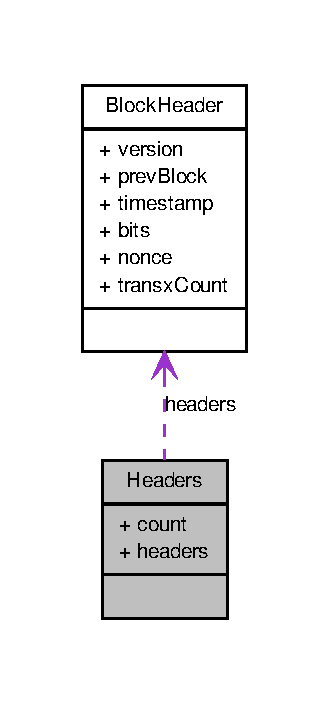
\includegraphics[width=158pt]{struct_headers__coll__graph}
\end{center}
\end{figure}
\subsection*{Data Fields}
\begin{DoxyCompactItemize}
\item 
long int \hyperlink{struct_headers_aabbb2f7768ed83b49f05e7911e3a693a}{count}
\item 
struct \hyperlink{struct_block_header}{BlockHeader} $\ast$ \hyperlink{struct_headers_a0b894950328debae0613f43ca1f0dc64}{headers}
\end{DoxyCompactItemize}


\subsection{Detailed Description}


Definition at line 195 of file Protocol.h.



\subsection{Field Documentation}
\hypertarget{struct_headers_aabbb2f7768ed83b49f05e7911e3a693a}{
\index{Headers@{Headers}!count@{count}}
\index{count@{count}!Headers@{Headers}}
\subsubsection[{count}]{\setlength{\rightskip}{0pt plus 5cm}long int {\bf count}}}
\label{struct_headers_aabbb2f7768ed83b49f05e7911e3a693a}


Definition at line 196 of file Protocol.h.

\hypertarget{struct_headers_a0b894950328debae0613f43ca1f0dc64}{
\index{Headers@{Headers}!headers@{headers}}
\index{headers@{headers}!Headers@{Headers}}
\subsubsection[{headers}]{\setlength{\rightskip}{0pt plus 5cm}struct {\bf BlockHeader}$\ast$ {\bf headers}}}
\label{struct_headers_a0b894950328debae0613f43ca1f0dc64}


Definition at line 197 of file Protocol.h.



The documentation for this struct was generated from the following file:\begin{DoxyCompactItemize}
\item 
src/Object/NetworkProtocol/\hyperlink{_protocol_8h}{Protocol.h}\end{DoxyCompactItemize}

\hypertarget{struct_header_spck}{
\section{HeaderSpck Struct Reference}
\label{struct_header_spck}\index{HeaderSpck@{HeaderSpck}}
}


{\ttfamily \#include $<$Protocol.h$>$}

\subsection*{Data Fields}
\begin{DoxyCompactItemize}
\item 
int \hyperlink{struct_header_spck_a9d86e57aaa1003de664fdbe3fe6bc35a}{startCount}
\item 
char \hyperlink{struct_header_spck_afb278e99e58307608e33751cd490c97b}{hashStart} \mbox{[}32\mbox{]}
\item 
char \hyperlink{struct_header_spck_aa16ea670ce42c626f461fc49f74ddcd3}{hashStop} \mbox{[}32\mbox{]}
\end{DoxyCompactItemize}


\subsection{Detailed Description}


Definition at line 137 of file Protocol.h.



\subsection{Field Documentation}
\hypertarget{struct_header_spck_afb278e99e58307608e33751cd490c97b}{
\index{HeaderSpck@{HeaderSpck}!hashStart@{hashStart}}
\index{hashStart@{hashStart}!HeaderSpck@{HeaderSpck}}
\subsubsection[{hashStart}]{\setlength{\rightskip}{0pt plus 5cm}char {\bf hashStart}\mbox{[}32\mbox{]}}}
\label{struct_header_spck_afb278e99e58307608e33751cd490c97b}


Definition at line 139 of file Protocol.h.

\hypertarget{struct_header_spck_aa16ea670ce42c626f461fc49f74ddcd3}{
\index{HeaderSpck@{HeaderSpck}!hashStop@{hashStop}}
\index{hashStop@{hashStop}!HeaderSpck@{HeaderSpck}}
\subsubsection[{hashStop}]{\setlength{\rightskip}{0pt plus 5cm}char {\bf hashStop}\mbox{[}32\mbox{]}}}
\label{struct_header_spck_aa16ea670ce42c626f461fc49f74ddcd3}


Definition at line 140 of file Protocol.h.

\hypertarget{struct_header_spck_a9d86e57aaa1003de664fdbe3fe6bc35a}{
\index{HeaderSpck@{HeaderSpck}!startCount@{startCount}}
\index{startCount@{startCount}!HeaderSpck@{HeaderSpck}}
\subsubsection[{startCount}]{\setlength{\rightskip}{0pt plus 5cm}int {\bf startCount}}}
\label{struct_header_spck_a9d86e57aaa1003de664fdbe3fe6bc35a}


Definition at line 138 of file Protocol.h.



The documentation for this struct was generated from the following file:\begin{DoxyCompactItemize}
\item 
src/Object/NetworkProtocol/\hyperlink{_protocol_8h}{Protocol.h}\end{DoxyCompactItemize}

\hypertarget{struct_inventory}{
\section{Inventory Struct Reference}
\label{struct_inventory}\index{Inventory@{Inventory}}
}


Structure for \hyperlink{struct_inventory}{Inventory} objects.  




{\ttfamily \#include $<$Inventory.h$>$}



Collaboration diagram for Inventory:
\nopagebreak
\begin{figure}[H]
\begin{center}
\leavevmode
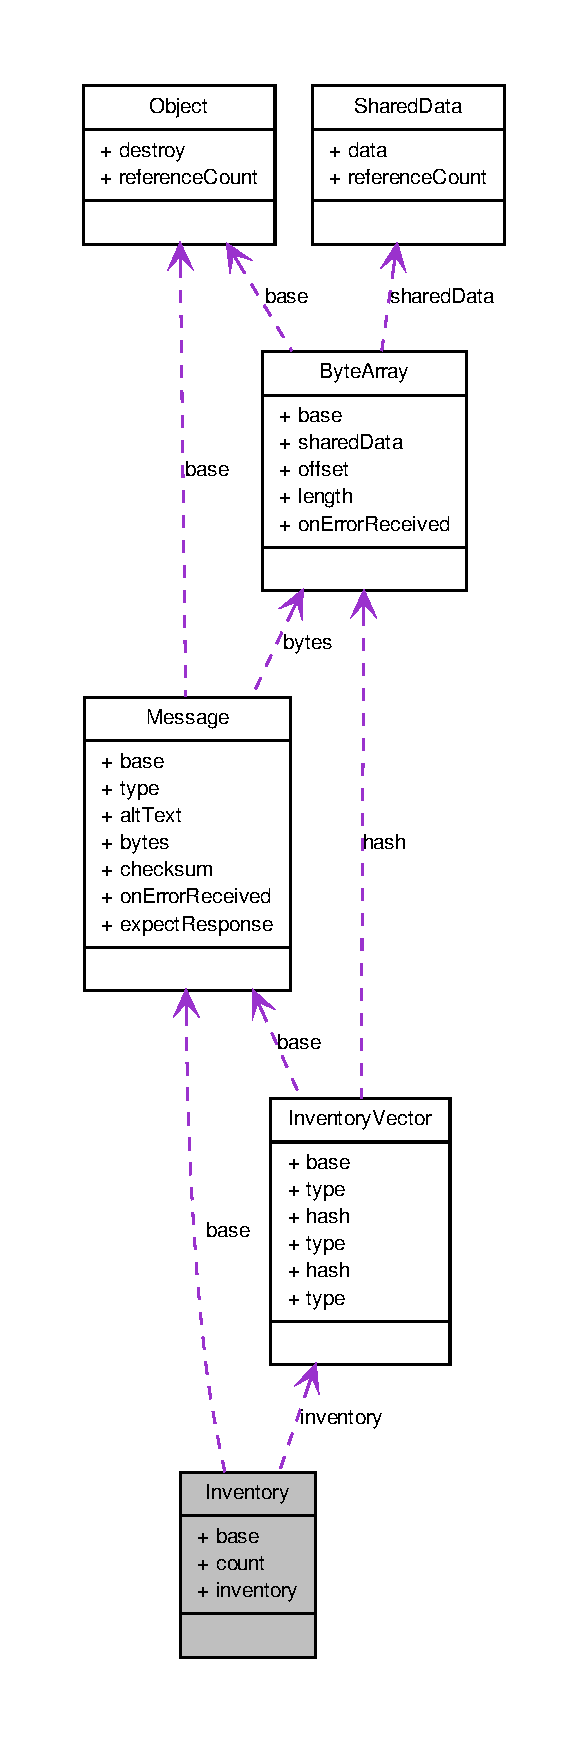
\includegraphics[height=600pt]{struct_inventory__coll__graph}
\end{center}
\end{figure}
\subsection*{Data Fields}
\begin{DoxyCompactItemize}
\item 
\hyperlink{struct_message}{Message} \hyperlink{struct_inventory_a8987f797adf70c3e174fd64cc68bc933}{base}
\item 
uint16\_\-t \hyperlink{struct_inventory_af6a39bfc7e1dc3b6f9c997c1c43fa996}{count}
\item 
\hyperlink{struct_inventory_vector}{InventoryVector} $\ast$$\ast$ \hyperlink{struct_inventory_a5434993362e4e5b940a640f34b3c417d}{inventory}
\end{DoxyCompactItemize}


\subsection{Detailed Description}
Structure for \hyperlink{struct_inventory}{Inventory} objects. 

\begin{DoxySeeAlso}{See also}
\hyperlink{_inventory_8h}{Inventory.h} 
\end{DoxySeeAlso}


Definition at line 26 of file Inventory.h.



\subsection{Field Documentation}
\hypertarget{struct_inventory_a8987f797adf70c3e174fd64cc68bc933}{
\index{Inventory@{Inventory}!base@{base}}
\index{base@{base}!Inventory@{Inventory}}
\subsubsection[{base}]{\setlength{\rightskip}{0pt plus 5cm}{\bf Message} {\bf base}}}
\label{struct_inventory_a8987f797adf70c3e174fd64cc68bc933}
\hyperlink{struct_message}{Message} base structure 

Definition at line 27 of file Inventory.h.

\hypertarget{struct_inventory_af6a39bfc7e1dc3b6f9c997c1c43fa996}{
\index{Inventory@{Inventory}!count@{count}}
\index{count@{count}!Inventory@{Inventory}}
\subsubsection[{count}]{\setlength{\rightskip}{0pt plus 5cm}uint16\_\-t {\bf count}}}
\label{struct_inventory_af6a39bfc7e1dc3b6f9c997c1c43fa996}
Number of inventory entries. 

Definition at line 28 of file Inventory.h.

\hypertarget{struct_inventory_a5434993362e4e5b940a640f34b3c417d}{
\index{Inventory@{Inventory}!inventory@{inventory}}
\index{inventory@{inventory}!Inventory@{Inventory}}
\subsubsection[{inventory}]{\setlength{\rightskip}{0pt plus 5cm}{\bf InventoryVector}$\ast$$\ast$ {\bf inventory}}}
\label{struct_inventory_a5434993362e4e5b940a640f34b3c417d}
The \hyperlink{struct_inventory}{Inventory} vectors. This should be a memory block of pointers to InventoryVectors. It will be freed when the \hyperlink{struct_inventory}{Inventory} is freed. When adding an item it should be retained. When removing an item it should be released. Leave or set as NULL if empty. 

Definition at line 29 of file Inventory.h.



The documentation for this struct was generated from the following file:\begin{DoxyCompactItemize}
\item 
src/Object/Message/\hyperlink{_inventory_8h}{Inventory.h}\end{DoxyCompactItemize}

\hypertarget{struct_inventory_vector}{
\section{InventoryVector Struct Reference}
\label{struct_inventory_vector}\index{InventoryVector@{InventoryVector}}
}


Structure for \hyperlink{struct_inventory_vector}{InventoryVector} objects.  




{\ttfamily \#include $<$InventoryVector.h$>$}



Collaboration diagram for InventoryVector:
\nopagebreak
\begin{figure}[H]
\begin{center}
\leavevmode
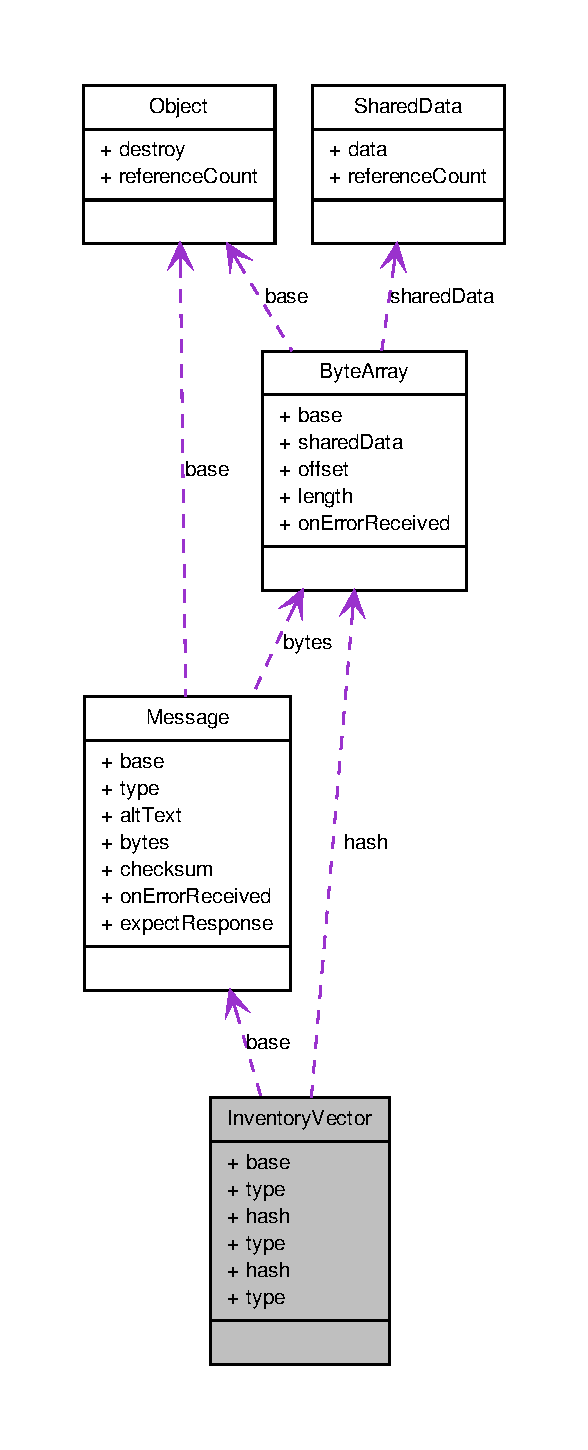
\includegraphics[height=600pt]{struct_inventory_vector__coll__graph}
\end{center}
\end{figure}
\subsection*{Data Fields}
\begin{DoxyCompactItemize}
\item 
\hyperlink{struct_message}{Message} \hyperlink{struct_inventory_vector_a8987f797adf70c3e174fd64cc68bc933}{base}
\item 
\hyperlink{_constants_8h_a540a9c34662db8bb84b729512cf08e75}{InventoryVectorType} \hyperlink{struct_inventory_vector_aae693fef743079289c6c94035f7aae77}{type}
\item 
\hyperlink{struct_byte_array}{ByteArray} $\ast$ \hyperlink{struct_inventory_vector_a5309b3103b4345688327148e3c589014}{hash}
\item 
uint32\_\-t \hyperlink{struct_inventory_vector_ad44b615021ed3ccb734fcaf583ef4a03}{type}
\item 
char \hyperlink{struct_inventory_vector_a30660ee1bca7189182e64c5a192651af}{hash} \mbox{[}32\mbox{]}
\item 
unsigned int \hyperlink{struct_inventory_vector_a4bfea42429249a1f65204f0c0f34704a}{type}
\end{DoxyCompactItemize}


\subsection{Detailed Description}
Structure for \hyperlink{struct_inventory_vector}{InventoryVector} objects. 

\begin{DoxySeeAlso}{See also}
\hyperlink{_inventory_vector_8h}{InventoryVector.h} 
\end{DoxySeeAlso}


Definition at line 23 of file InventoryVector.h.



\subsection{Field Documentation}
\hypertarget{struct_inventory_vector_a8987f797adf70c3e174fd64cc68bc933}{
\index{InventoryVector@{InventoryVector}!base@{base}}
\index{base@{base}!InventoryVector@{InventoryVector}}
\subsubsection[{base}]{\setlength{\rightskip}{0pt plus 5cm}{\bf Message} {\bf base}}}
\label{struct_inventory_vector_a8987f797adf70c3e174fd64cc68bc933}
\hyperlink{struct_message}{Message} base structure 

Definition at line 24 of file InventoryVector.h.

\hypertarget{struct_inventory_vector_a30660ee1bca7189182e64c5a192651af}{
\index{InventoryVector@{InventoryVector}!hash@{hash}}
\index{hash@{hash}!InventoryVector@{InventoryVector}}
\subsubsection[{hash}]{\setlength{\rightskip}{0pt plus 5cm}char {\bf hash}\mbox{[}32\mbox{]}}}
\label{struct_inventory_vector_a30660ee1bca7189182e64c5a192651af}


Definition at line 32 of file Commands.h.

\hypertarget{struct_inventory_vector_a5309b3103b4345688327148e3c589014}{
\index{InventoryVector@{InventoryVector}!hash@{hash}}
\index{hash@{hash}!InventoryVector@{InventoryVector}}
\subsubsection[{hash}]{\setlength{\rightskip}{0pt plus 5cm}char {\bf hash}}}
\label{struct_inventory_vector_a5309b3103b4345688327148e3c589014}
The hash of the inventory vector 

Definition at line 26 of file InventoryVector.h.

\hypertarget{struct_inventory_vector_ad44b615021ed3ccb734fcaf583ef4a03}{
\index{InventoryVector@{InventoryVector}!type@{type}}
\index{type@{type}!InventoryVector@{InventoryVector}}
\subsubsection[{type}]{\setlength{\rightskip}{0pt plus 5cm}uint32\_\-t {\bf type}}}
\label{struct_inventory_vector_ad44b615021ed3ccb734fcaf583ef4a03}


Definition at line 30 of file Commands.h.

\hypertarget{struct_inventory_vector_aae693fef743079289c6c94035f7aae77}{
\index{InventoryVector@{InventoryVector}!type@{type}}
\index{type@{type}!InventoryVector@{InventoryVector}}
\subsubsection[{type}]{\setlength{\rightskip}{0pt plus 5cm}{\bf InventoryVectorType} {\bf type}}}
\label{struct_inventory_vector_aae693fef743079289c6c94035f7aae77}
The type of the inventory vector. It can be an error, a transaction or a block 

Definition at line 25 of file InventoryVector.h.

\hypertarget{struct_inventory_vector_a4bfea42429249a1f65204f0c0f34704a}{
\index{InventoryVector@{InventoryVector}!type@{type}}
\index{type@{type}!InventoryVector@{InventoryVector}}
\subsubsection[{type}]{\setlength{\rightskip}{0pt plus 5cm}unsigned int {\bf type}}}
\label{struct_inventory_vector_a4bfea42429249a1f65204f0c0f34704a}


Definition at line 114 of file Protocol.h.



The documentation for this struct was generated from the following files:\begin{DoxyCompactItemize}
\item 
src/Object/Message/\hyperlink{_inventory_vector_8h}{InventoryVector.h}\item 
src/Object/NetworkProtocol/\hyperlink{_commands_8h}{Commands.h}\item 
src/Object/NetworkProtocol/\hyperlink{_protocol_8h}{Protocol.h}\end{DoxyCompactItemize}

\hypertarget{struct_irc_addr}{
\section{IrcAddr Struct Reference}
\label{struct_irc_addr}\index{IrcAddr@{IrcAddr}}
}


{\ttfamily \#include $<$Protocol.h$>$}

\subsection*{Data Fields}
\begin{DoxyCompactItemize}
\item 
int \hyperlink{struct_irc_addr_addd335afdb9230f431842ebb6cbbce62}{ip}
\item 
short \hyperlink{struct_irc_addr_aee6a7f5f7c1e964cbd84deec9c53ba15}{port}
\end{DoxyCompactItemize}


\subsection{Detailed Description}


Definition at line 20 of file Protocol.h.



\subsection{Field Documentation}
\hypertarget{struct_irc_addr_addd335afdb9230f431842ebb6cbbce62}{
\index{IrcAddr@{IrcAddr}!ip@{ip}}
\index{ip@{ip}!IrcAddr@{IrcAddr}}
\subsubsection[{ip}]{\setlength{\rightskip}{0pt plus 5cm}int {\bf ip}}}
\label{struct_irc_addr_addd335afdb9230f431842ebb6cbbce62}


Definition at line 22 of file Protocol.h.

\hypertarget{struct_irc_addr_aee6a7f5f7c1e964cbd84deec9c53ba15}{
\index{IrcAddr@{IrcAddr}!port@{port}}
\index{port@{port}!IrcAddr@{IrcAddr}}
\subsubsection[{port}]{\setlength{\rightskip}{0pt plus 5cm}short {\bf port}}}
\label{struct_irc_addr_aee6a7f5f7c1e964cbd84deec9c53ba15}


Definition at line 23 of file Protocol.h.



The documentation for this struct was generated from the following file:\begin{DoxyCompactItemize}
\item 
src/Object/NetworkProtocol/\hyperlink{_protocol_8h}{Protocol.h}\end{DoxyCompactItemize}

\hypertarget{struct_merkle_node}{
\section{MerkleNode Struct Reference}
\label{struct_merkle_node}\index{MerkleNode@{MerkleNode}}
}


{\ttfamily \#include $<$MerkleNode.h$>$}



Collaboration diagram for MerkleNode:\nopagebreak
\begin{figure}[H]
\begin{center}
\leavevmode
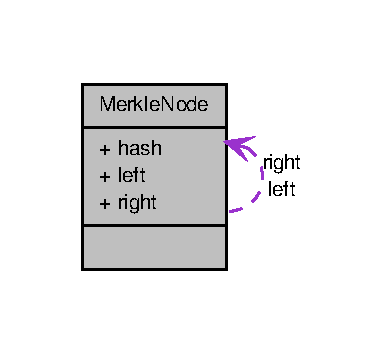
\includegraphics[width=185pt]{struct_merkle_node__coll__graph}
\end{center}
\end{figure}
\subsection*{Data Fields}
\begin{DoxyCompactItemize}
\item 
uint8\_\-t \hyperlink{struct_merkle_node_a7ff9da008bf055da1f1ba994c562057d}{hash} \mbox{[}32\mbox{]}
\item 
\hyperlink{struct_merkle_node}{MerkleNode} $\ast$ \hyperlink{struct_merkle_node_a3292e1ae6fbbb8666d2007bee45b69a1}{left}
\item 
\hyperlink{struct_merkle_node}{MerkleNode} $\ast$ \hyperlink{struct_merkle_node_a131f273991e1615aab021dd945479c62}{right}
\end{DoxyCompactItemize}


\subsection{Detailed Description}
\begin{DoxySeeAlso}{See also}
\hyperlink{_merkle_node_8h}{MerkleNode.h} 
\end{DoxySeeAlso}


Definition at line 25 of file MerkleNode.h.



\subsection{Field Documentation}
\hypertarget{struct_merkle_node_a7ff9da008bf055da1f1ba994c562057d}{
\index{MerkleNode@{MerkleNode}!hash@{hash}}
\index{hash@{hash}!MerkleNode@{MerkleNode}}
\subsubsection[{hash}]{\setlength{\rightskip}{0pt plus 5cm}uint8\_\-t {\bf hash}\mbox{[}32\mbox{]}}}
\label{struct_merkle_node_a7ff9da008bf055da1f1ba994c562057d}
The hash for this node. 

Definition at line 26 of file MerkleNode.h.

\hypertarget{struct_merkle_node_a3292e1ae6fbbb8666d2007bee45b69a1}{
\index{MerkleNode@{MerkleNode}!left@{left}}
\index{left@{left}!MerkleNode@{MerkleNode}}
\subsubsection[{left}]{\setlength{\rightskip}{0pt plus 5cm}{\bf MerkleNode}$\ast$ {\bf left}}}
\label{struct_merkle_node_a3292e1ae6fbbb8666d2007bee45b69a1}
The left child. NULL if leaf. 

Definition at line 27 of file MerkleNode.h.

\hypertarget{struct_merkle_node_a131f273991e1615aab021dd945479c62}{
\index{MerkleNode@{MerkleNode}!right@{right}}
\index{right@{right}!MerkleNode@{MerkleNode}}
\subsubsection[{right}]{\setlength{\rightskip}{0pt plus 5cm}{\bf MerkleNode}$\ast$ {\bf right}}}
\label{struct_merkle_node_a131f273991e1615aab021dd945479c62}
The right child. NULL if leaf. 

Definition at line 28 of file MerkleNode.h.



The documentation for this struct was generated from the following file:\begin{DoxyCompactItemize}
\item 
src/MerkleNode/\hyperlink{_merkle_node_8h}{MerkleNode.h}\end{DoxyCompactItemize}

\hypertarget{struct_message}{
\section{Message Struct Reference}
\label{struct_message}\index{Message@{Message}}
}


Structure for \hyperlink{struct_message}{Message} objects.  




{\ttfamily \#include $<$Message.h$>$}



Collaboration diagram for Message:\nopagebreak
\begin{figure}[H]
\begin{center}
\leavevmode
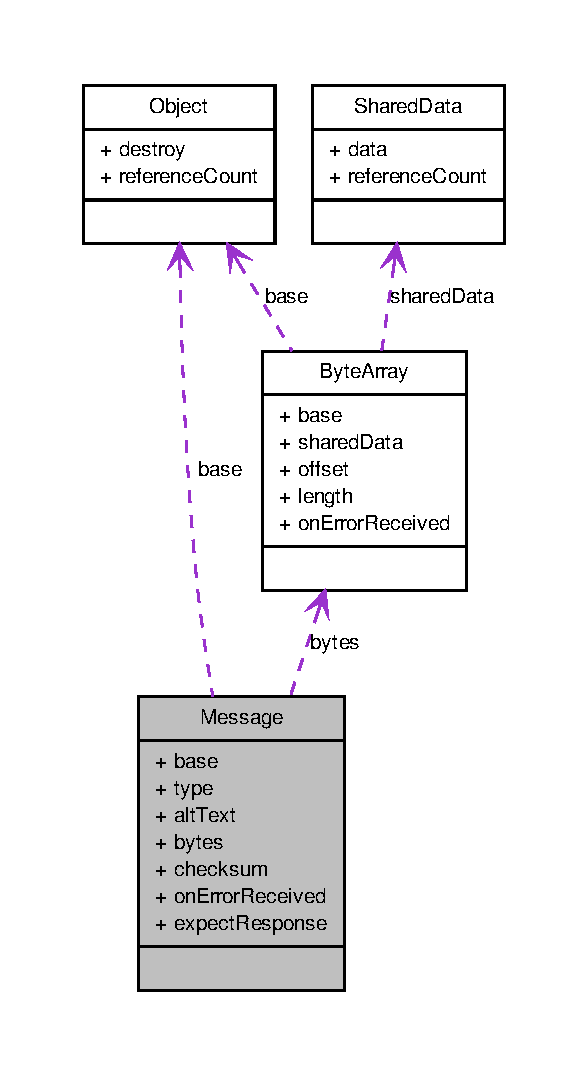
\includegraphics[width=282pt]{struct_message__coll__graph}
\end{center}
\end{figure}
\subsection*{Data Fields}
\begin{DoxyCompactItemize}
\item 
\hyperlink{struct_object}{Object} \hyperlink{struct_message_a23cf4ef56ba22bed625eab08d6361fa7}{base}
\item 
\hyperlink{_constants_8h_ac6606ebe91c8ac66a2c314c79f5ab013}{MessageType} \hyperlink{struct_message_a8a2053c7fb1adf60da2f26c06059539e}{type}
\item 
uint8\_\-t $\ast$ \hyperlink{struct_message_ad4a1b71852a8721ee4be4f6aaacd8566}{altText}
\item 
\hyperlink{struct_byte_array}{ByteArray} $\ast$ \hyperlink{struct_message_affc357b616afe9b58c190ae4b21caa77}{bytes}
\item 
uint8\_\-t \hyperlink{struct_message_a02d93e565ee31bda6e0211dca9b42be5}{checksum} \mbox{[}4\mbox{]}
\item 
void($\ast$ \hyperlink{struct_message_a3c8af4f580f3041d046b7581f89a9695}{onErrorReceived} )(\hyperlink{_constants_8h_a2c3e4bb40f36b262a5214e2da2bca9c5}{Error} error, char $\ast$,...)
\item 
\hyperlink{_constants_8h_ac6606ebe91c8ac66a2c314c79f5ab013}{MessageType} \hyperlink{struct_message_accc3616411ea4a5035a7eaf42132d370}{expectResponse}
\end{DoxyCompactItemize}


\subsection{Detailed Description}
Structure for \hyperlink{struct_message}{Message} objects. 

\begin{DoxySeeAlso}{See also}
\hyperlink{_message_8h}{Message.h} 
\end{DoxySeeAlso}


Definition at line 29 of file Message.h.



\subsection{Field Documentation}
\hypertarget{struct_message_ad4a1b71852a8721ee4be4f6aaacd8566}{
\index{Message@{Message}!altText@{altText}}
\index{altText@{altText}!Message@{Message}}
\subsubsection[{altText}]{\setlength{\rightskip}{0pt plus 5cm}uint8\_\-t$\ast$ {\bf altText}}}
\label{struct_message_ad4a1b71852a8721ee4be4f6aaacd8566}
For an alternative message: This is the type text. 

Definition at line 32 of file Message.h.

\hypertarget{struct_message_a23cf4ef56ba22bed625eab08d6361fa7}{
\index{Message@{Message}!base@{base}}
\index{base@{base}!Message@{Message}}
\subsubsection[{base}]{\setlength{\rightskip}{0pt plus 5cm}{\bf Object} {\bf base}}}
\label{struct_message_a23cf4ef56ba22bed625eab08d6361fa7}
\hyperlink{struct_object}{Object} base structure 

Definition at line 30 of file Message.h.

\hypertarget{struct_message_affc357b616afe9b58c190ae4b21caa77}{
\index{Message@{Message}!bytes@{bytes}}
\index{bytes@{bytes}!Message@{Message}}
\subsubsection[{bytes}]{\setlength{\rightskip}{0pt plus 5cm}{\bf ByteArray}$\ast$ {\bf bytes}}}
\label{struct_message_affc357b616afe9b58c190ae4b21caa77}
Raw message data minus the message header. When serialising this should be assigned to a \hyperlink{struct_byte_array}{ByteArray} large enough to hold the serialised data. 

Definition at line 33 of file Message.h.

\hypertarget{struct_message_a02d93e565ee31bda6e0211dca9b42be5}{
\index{Message@{Message}!checksum@{checksum}}
\index{checksum@{checksum}!Message@{Message}}
\subsubsection[{checksum}]{\setlength{\rightskip}{0pt plus 5cm}uint8\_\-t {\bf checksum}\mbox{[}4\mbox{]}}}
\label{struct_message_a02d93e565ee31bda6e0211dca9b42be5}
The message checksum. When sending messages using a NetworkCommunicator, this is calculated for you. 

Definition at line 34 of file Message.h.

\hypertarget{struct_message_accc3616411ea4a5035a7eaf42132d370}{
\index{Message@{Message}!expectResponse@{expectResponse}}
\index{expectResponse@{expectResponse}!Message@{Message}}
\subsubsection[{expectResponse}]{\setlength{\rightskip}{0pt plus 5cm}{\bf MessageType} {\bf expectResponse}}}
\label{struct_message_accc3616411ea4a5035a7eaf42132d370}
Set to zero if no message expected or the type of message expected as a response. 

Definition at line 36 of file Message.h.

\hypertarget{struct_message_a3c8af4f580f3041d046b7581f89a9695}{
\index{Message@{Message}!onErrorReceived@{onErrorReceived}}
\index{onErrorReceived@{onErrorReceived}!Message@{Message}}
\subsubsection[{onErrorReceived}]{\setlength{\rightskip}{0pt plus 5cm}void($\ast$ {\bf onErrorReceived})({\bf Error} error, char $\ast$,...)}}
\label{struct_message_a3c8af4f580f3041d046b7581f89a9695}
Pointer to error callback 

Definition at line 35 of file Message.h.

\hypertarget{struct_message_a8a2053c7fb1adf60da2f26c06059539e}{
\index{Message@{Message}!type@{type}}
\index{type@{type}!Message@{Message}}
\subsubsection[{type}]{\setlength{\rightskip}{0pt plus 5cm}{\bf MessageType} {\bf type}}}
\label{struct_message_a8a2053c7fb1adf60da2f26c06059539e}
The type of the message 

Definition at line 31 of file Message.h.



The documentation for this struct was generated from the following file:\begin{DoxyCompactItemize}
\item 
src/Object/Message/\hyperlink{_message_8h}{Message.h}\end{DoxyCompactItemize}

\hypertarget{structmy_class}{
\section{myClass Struct Reference}
\label{structmy_class}\index{myClass@{myClass}}
}
\subsection*{Data Fields}
\begin{DoxyCompactItemize}
\item 
int \hyperlink{structmy_class_a7441ef0865bcb3db9b8064dd7375c1ea}{id}
\item 
char $\ast$ \hyperlink{structmy_class_a5ac083a645d964373f022d03df4849c8}{name}
\end{DoxyCompactItemize}


\subsection{Detailed Description}


Definition at line 6 of file IbTest.c.



\subsection{Field Documentation}
\hypertarget{structmy_class_a7441ef0865bcb3db9b8064dd7375c1ea}{
\index{myClass@{myClass}!id@{id}}
\index{id@{id}!myClass@{myClass}}
\subsubsection[{id}]{\setlength{\rightskip}{0pt plus 5cm}int {\bf id}}}
\label{structmy_class_a7441ef0865bcb3db9b8064dd7375c1ea}


Definition at line 7 of file IbTest.c.

\hypertarget{structmy_class_a5ac083a645d964373f022d03df4849c8}{
\index{myClass@{myClass}!name@{name}}
\index{name@{name}!myClass@{myClass}}
\subsubsection[{name}]{\setlength{\rightskip}{0pt plus 5cm}char$\ast$ {\bf name}}}
\label{structmy_class_a5ac083a645d964373f022d03df4849c8}


Definition at line 8 of file IbTest.c.



The documentation for this struct was generated from the following file:\begin{DoxyCompactItemize}
\item 
src/\hyperlink{_ib_test_8c}{IbTest.c}\end{DoxyCompactItemize}

\hypertarget{struct_net_addr}{
\section{NetAddr Struct Reference}
\label{struct_net_addr}\index{NetAddr@{NetAddr}}
}


{\ttfamily \#include $<$Protocol.h$>$}

\subsection*{Data Fields}
\begin{DoxyCompactItemize}
\item 
unsigned int \hyperlink{struct_net_addr_a83e57ce9bd59cfa0995c2e2c8589c274}{time}
\item 
long int \hyperlink{struct_net_addr_a7c2c2697560cb0d08fdca3bd4d10d07e}{services}
\item 
unsigned char \hyperlink{struct_net_addr_a9799580e054ff5683ffbeb32502f7475}{ip} \mbox{[}16\mbox{]}
\item 
unsigned short \hyperlink{struct_net_addr_ab85ff85aa1f60f4a1c1ca1225a9dad06}{port}
\end{DoxyCompactItemize}


\subsection{Detailed Description}


Definition at line 29 of file Protocol.h.



\subsection{Field Documentation}
\hypertarget{struct_net_addr_a9799580e054ff5683ffbeb32502f7475}{
\index{NetAddr@{NetAddr}!ip@{ip}}
\index{ip@{ip}!NetAddr@{NetAddr}}
\subsubsection[{ip}]{\setlength{\rightskip}{0pt plus 5cm}unsigned char {\bf ip}\mbox{[}16\mbox{]}}}
\label{struct_net_addr_a9799580e054ff5683ffbeb32502f7475}


Definition at line 33 of file Protocol.h.

\hypertarget{struct_net_addr_ab85ff85aa1f60f4a1c1ca1225a9dad06}{
\index{NetAddr@{NetAddr}!port@{port}}
\index{port@{port}!NetAddr@{NetAddr}}
\subsubsection[{port}]{\setlength{\rightskip}{0pt plus 5cm}unsigned short {\bf port}}}
\label{struct_net_addr_ab85ff85aa1f60f4a1c1ca1225a9dad06}


Definition at line 34 of file Protocol.h.

\hypertarget{struct_net_addr_a7c2c2697560cb0d08fdca3bd4d10d07e}{
\index{NetAddr@{NetAddr}!services@{services}}
\index{services@{services}!NetAddr@{NetAddr}}
\subsubsection[{services}]{\setlength{\rightskip}{0pt plus 5cm}long int {\bf services}}}
\label{struct_net_addr_a7c2c2697560cb0d08fdca3bd4d10d07e}


Definition at line 32 of file Protocol.h.

\hypertarget{struct_net_addr_a83e57ce9bd59cfa0995c2e2c8589c274}{
\index{NetAddr@{NetAddr}!time@{time}}
\index{time@{time}!NetAddr@{NetAddr}}
\subsubsection[{time}]{\setlength{\rightskip}{0pt plus 5cm}unsigned int {\bf time}}}
\label{struct_net_addr_a83e57ce9bd59cfa0995c2e2c8589c274}


Definition at line 31 of file Protocol.h.



The documentation for this struct was generated from the following file:\begin{DoxyCompactItemize}
\item 
src/Object/NetworkProtocol/\hyperlink{_protocol_8h}{Protocol.h}\end{DoxyCompactItemize}

\hypertarget{struct_network_address}{
\section{NetworkAddress Struct Reference}
\label{struct_network_address}\index{NetworkAddress@{NetworkAddress}}
}


{\ttfamily \#include $<$Commands.h$>$}

\subsection*{Data Fields}
\begin{DoxyCompactItemize}
\item 
uint32\_\-t \hyperlink{struct_network_address_ae73654f333e4363463ad8c594eca1905}{time}
\item 
uint64\_\-t \hyperlink{struct_network_address_a8361260b2ca75771b8da0333191db456}{services}
\item 
char \hyperlink{struct_network_address_ac03ec605186c0c6d17c4beaab73d615c}{ip} \mbox{[}16\mbox{]}
\item 
uint16\_\-t \hyperlink{struct_network_address_a8e0798404bf2cf5dabb84c5ba9a4f236}{port}
\end{DoxyCompactItemize}


\subsection{Detailed Description}


Definition at line 21 of file Commands.h.



\subsection{Field Documentation}
\hypertarget{struct_network_address_ac03ec605186c0c6d17c4beaab73d615c}{
\index{NetworkAddress@{NetworkAddress}!ip@{ip}}
\index{ip@{ip}!NetworkAddress@{NetworkAddress}}
\subsubsection[{ip}]{\setlength{\rightskip}{0pt plus 5cm}char {\bf ip}\mbox{[}16\mbox{]}}}
\label{struct_network_address_ac03ec605186c0c6d17c4beaab73d615c}


Definition at line 24 of file Commands.h.

\hypertarget{struct_network_address_a8e0798404bf2cf5dabb84c5ba9a4f236}{
\index{NetworkAddress@{NetworkAddress}!port@{port}}
\index{port@{port}!NetworkAddress@{NetworkAddress}}
\subsubsection[{port}]{\setlength{\rightskip}{0pt plus 5cm}uint16\_\-t {\bf port}}}
\label{struct_network_address_a8e0798404bf2cf5dabb84c5ba9a4f236}


Definition at line 25 of file Commands.h.

\hypertarget{struct_network_address_a8361260b2ca75771b8da0333191db456}{
\index{NetworkAddress@{NetworkAddress}!services@{services}}
\index{services@{services}!NetworkAddress@{NetworkAddress}}
\subsubsection[{services}]{\setlength{\rightskip}{0pt plus 5cm}uint64\_\-t {\bf services}}}
\label{struct_network_address_a8361260b2ca75771b8da0333191db456}


Definition at line 23 of file Commands.h.

\hypertarget{struct_network_address_ae73654f333e4363463ad8c594eca1905}{
\index{NetworkAddress@{NetworkAddress}!time@{time}}
\index{time@{time}!NetworkAddress@{NetworkAddress}}
\subsubsection[{time}]{\setlength{\rightskip}{0pt plus 5cm}uint32\_\-t {\bf time}}}
\label{struct_network_address_ae73654f333e4363463ad8c594eca1905}


Definition at line 22 of file Commands.h.



The documentation for this struct was generated from the following file:\begin{DoxyCompactItemize}
\item 
src/Object/NetworkProtocol/\hyperlink{_commands_8h}{Commands.h}\end{DoxyCompactItemize}

\hypertarget{struct_node_discovery}{
\section{NodeDiscovery Struct Reference}
\label{struct_node_discovery}\index{NodeDiscovery@{NodeDiscovery}}
}


Structure for \hyperlink{struct_node_discovery}{NodeDiscovery} objects.  




{\ttfamily \#include $<$NodeDiscovery.h$>$}



Collaboration diagram for NodeDiscovery:\nopagebreak
\begin{figure}[H]
\begin{center}
\leavevmode
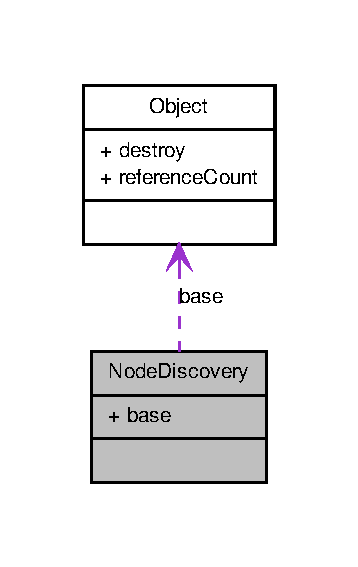
\includegraphics[width=172pt]{struct_node_discovery__coll__graph}
\end{center}
\end{figure}
\subsection*{Data Fields}
\begin{DoxyCompactItemize}
\item 
\hyperlink{struct_object}{Object} \hyperlink{struct_node_discovery_a23cf4ef56ba22bed625eab08d6361fa7}{base}
\end{DoxyCompactItemize}


\subsection{Detailed Description}
Structure for \hyperlink{struct_node_discovery}{NodeDiscovery} objects. 

\begin{DoxySeeAlso}{See also}
\hyperlink{_node_discovery_8h}{NodeDiscovery.h} 
\end{DoxySeeAlso}


Definition at line 32 of file NodeDiscovery.h.



\subsection{Field Documentation}
\hypertarget{struct_node_discovery_a23cf4ef56ba22bed625eab08d6361fa7}{
\index{NodeDiscovery@{NodeDiscovery}!base@{base}}
\index{base@{base}!NodeDiscovery@{NodeDiscovery}}
\subsubsection[{base}]{\setlength{\rightskip}{0pt plus 5cm}{\bf Object} {\bf base}}}
\label{struct_node_discovery_a23cf4ef56ba22bed625eab08d6361fa7}
\hyperlink{struct_object}{Object} base structure 

Definition at line 33 of file NodeDiscovery.h.



The documentation for this struct was generated from the following file:\begin{DoxyCompactItemize}
\item 
src/Object/NodeDiscovery/\hyperlink{_node_discovery_8h}{NodeDiscovery.h}\end{DoxyCompactItemize}

\hypertarget{struct_object}{
\section{Object Struct Reference}
\label{struct_object}\index{Object@{Object}}
}


Base class.  




{\ttfamily \#include $<$Object.h$>$}

\subsection*{Data Fields}
\begin{DoxyCompactItemize}
\item 
void($\ast$ \hyperlink{struct_object_aa353725933e843001d4feb03f8268121}{destroy} )(void $\ast$)
\item 
uint32\_\-t \hyperlink{struct_object_ad83c3d5d3f46e6278a77cb80eb2a0705}{referenceCount}
\end{DoxyCompactItemize}


\subsection{Detailed Description}
Base class. 

Definition at line 28 of file Object.h.



\subsection{Field Documentation}
\hypertarget{struct_object_aa353725933e843001d4feb03f8268121}{
\index{Object@{Object}!destroy@{destroy}}
\index{destroy@{destroy}!Object@{Object}}
\subsubsection[{destroy}]{\setlength{\rightskip}{0pt plus 5cm}void($\ast$ {\bf destroy})(void $\ast$)}}
\label{struct_object_aa353725933e843001d4feb03f8268121}
Pointer to function for destroying the \hyperlink{struct_object}{Object} 

Definition at line 29 of file Object.h.

\hypertarget{struct_object_ad83c3d5d3f46e6278a77cb80eb2a0705}{
\index{Object@{Object}!referenceCount@{referenceCount}}
\index{referenceCount@{referenceCount}!Object@{Object}}
\subsubsection[{referenceCount}]{\setlength{\rightskip}{0pt plus 5cm}uint32\_\-t {\bf referenceCount}}}
\label{struct_object_ad83c3d5d3f46e6278a77cb80eb2a0705}
Number of references to this \hyperlink{struct_object}{Object} 

Definition at line 30 of file Object.h.



The documentation for this struct was generated from the following file:\begin{DoxyCompactItemize}
\item 
src/Object/\hyperlink{_object_8h}{Object.h}\end{DoxyCompactItemize}

\hypertarget{struct_outpoint}{
\section{Outpoint Struct Reference}
\label{struct_outpoint}\index{Outpoint@{Outpoint}}
}


{\ttfamily \#include $<$Commands.h$>$}

\subsection*{Data Fields}
\begin{DoxyCompactItemize}
\item 
char \hyperlink{struct_outpoint_a49e83595c89cca1c8cd37b9af318a908}{hash} \mbox{[}32\mbox{]}
\item 
uint32\_\-t \hyperlink{struct_outpoint_aafd95f8c7a99b9189ede7cdf0871ebe8}{index}
\item 
unsigned int \hyperlink{struct_outpoint_a589d64202487f78e3cc30dd2e04c5201}{index}
\end{DoxyCompactItemize}


\subsection{Detailed Description}


Definition at line 43 of file Commands.h.



\subsection{Field Documentation}
\hypertarget{struct_outpoint_a49e83595c89cca1c8cd37b9af318a908}{
\index{Outpoint@{Outpoint}!hash@{hash}}
\index{hash@{hash}!Outpoint@{Outpoint}}
\subsubsection[{hash}]{\setlength{\rightskip}{0pt plus 5cm}char {\bf hash}}}
\label{struct_outpoint_a49e83595c89cca1c8cd37b9af318a908}


Definition at line 44 of file Commands.h.

\hypertarget{struct_outpoint_a589d64202487f78e3cc30dd2e04c5201}{
\index{Outpoint@{Outpoint}!index@{index}}
\index{index@{index}!Outpoint@{Outpoint}}
\subsubsection[{index}]{\setlength{\rightskip}{0pt plus 5cm}unsigned int {\bf index}}}
\label{struct_outpoint_a589d64202487f78e3cc30dd2e04c5201}


Definition at line 148 of file Protocol.h.

\hypertarget{struct_outpoint_aafd95f8c7a99b9189ede7cdf0871ebe8}{
\index{Outpoint@{Outpoint}!index@{index}}
\index{index@{index}!Outpoint@{Outpoint}}
\subsubsection[{index}]{\setlength{\rightskip}{0pt plus 5cm}uint32\_\-t {\bf index}}}
\label{struct_outpoint_aafd95f8c7a99b9189ede7cdf0871ebe8}


Definition at line 45 of file Commands.h.



The documentation for this struct was generated from the following files:\begin{DoxyCompactItemize}
\item 
src/Object/NetworkProtocol/\hyperlink{_commands_8h}{Commands.h}\item 
src/Object/NetworkProtocol/\hyperlink{_protocol_8h}{Protocol.h}\end{DoxyCompactItemize}

\hypertarget{struct_ping_pong_message}{
\section{PingPongMessage Struct Reference}
\label{struct_ping_pong_message}\index{PingPongMessage@{PingPongMessage}}
}


Structure for \hyperlink{struct_ping_pong_message}{PingPongMessage} objects.  




{\ttfamily \#include $<$PingPongMessage.h$>$}



Collaboration diagram for PingPongMessage:
\nopagebreak
\begin{figure}[H]
\begin{center}
\leavevmode
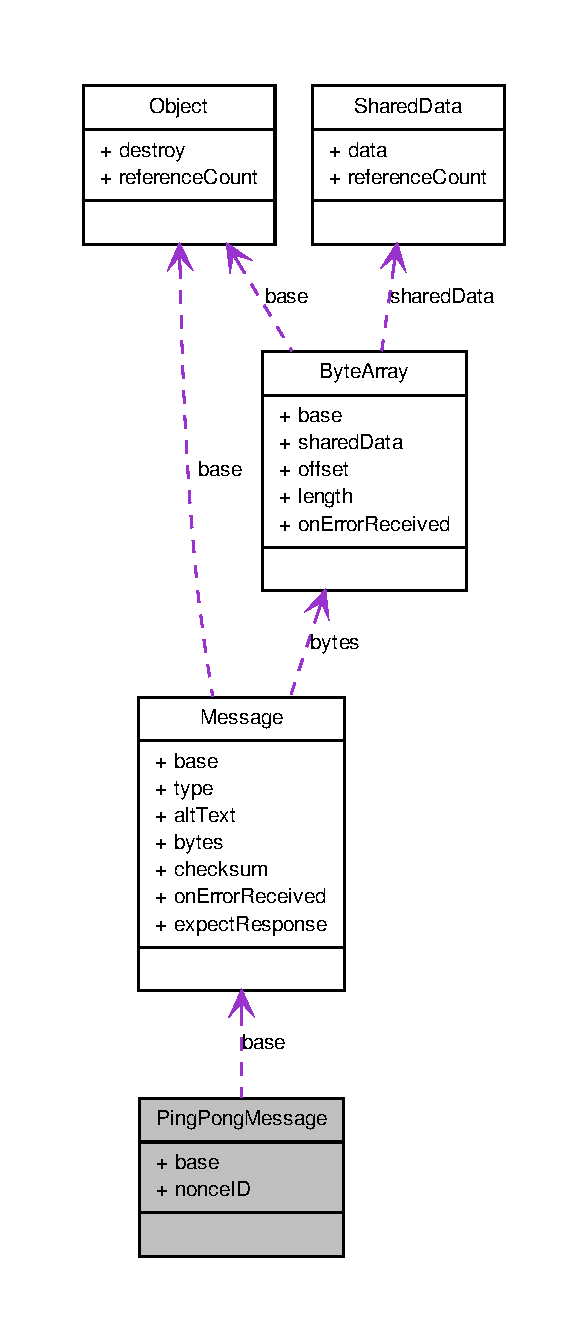
\includegraphics[height=600pt]{struct_ping_pong_message__coll__graph}
\end{center}
\end{figure}
\subsection*{Data Fields}
\begin{DoxyCompactItemize}
\item 
\hyperlink{struct_message}{Message} \hyperlink{struct_ping_pong_message_a8987f797adf70c3e174fd64cc68bc933}{base}
\item 
uint64\_\-t \hyperlink{struct_ping_pong_message_a8a30b0f39810620d125df55c023c996e}{nonceID}
\end{DoxyCompactItemize}


\subsection{Detailed Description}
Structure for \hyperlink{struct_ping_pong_message}{PingPongMessage} objects. 

\begin{DoxySeeAlso}{See also}
\hyperlink{_ping_pong_message_8h}{PingPongMessage.h} 
\end{DoxySeeAlso}


Definition at line 28 of file PingPongMessage.h.



\subsection{Field Documentation}
\hypertarget{struct_ping_pong_message_a8987f797adf70c3e174fd64cc68bc933}{
\index{PingPongMessage@{PingPongMessage}!base@{base}}
\index{base@{base}!PingPongMessage@{PingPongMessage}}
\subsubsection[{base}]{\setlength{\rightskip}{0pt plus 5cm}{\bf Message} {\bf base}}}
\label{struct_ping_pong_message_a8987f797adf70c3e174fd64cc68bc933}
\hyperlink{struct_message}{Message} base structure 

Definition at line 29 of file PingPongMessage.h.

\hypertarget{struct_ping_pong_message_a8a30b0f39810620d125df55c023c996e}{
\index{PingPongMessage@{PingPongMessage}!nonceID@{nonceID}}
\index{nonceID@{nonceID}!PingPongMessage@{PingPongMessage}}
\subsubsection[{nonceID}]{\setlength{\rightskip}{0pt plus 5cm}uint64\_\-t {\bf nonceID}}}
\label{struct_ping_pong_message_a8a30b0f39810620d125df55c023c996e}
Used to identify a ping/pong. Set ping to zero if no identification is needed. Set pongs to the same as the request ping. 

Definition at line 30 of file PingPongMessage.h.



The documentation for this struct was generated from the following file:\begin{DoxyCompactItemize}
\item 
src/Object/Message/\hyperlink{_ping_pong_message_8h}{PingPongMessage.h}\end{DoxyCompactItemize}

\hypertarget{struct_previous_output}{
\section{PreviousOutput Struct Reference}
\label{struct_previous_output}\index{PreviousOutput@{PreviousOutput}}
}


contains hash of the transaction and the number of outputs. Example of the structure: \{ hash: \char`\"{}0000000000000000000000000000000000000000000000000000000000000000\char`\"{}, n: 4294967295 \}  




{\ttfamily \#include $<$TransactionInput.h$>$}



Collaboration diagram for PreviousOutput:\nopagebreak
\begin{figure}[H]
\begin{center}
\leavevmode
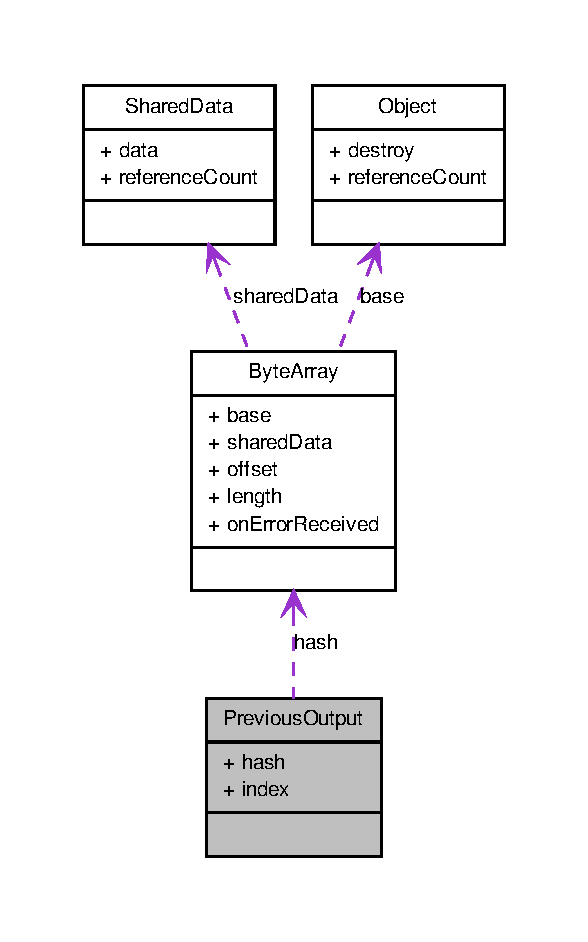
\includegraphics[width=282pt]{struct_previous_output__coll__graph}
\end{center}
\end{figure}
\subsection*{Data Fields}
\begin{DoxyCompactItemize}
\item 
\hyperlink{struct_byte_array}{ByteArray} $\ast$ \hyperlink{struct_previous_output_a5695540112ce950745e15ab422b3f067}{hash}
\item 
uint32\_\-t \hyperlink{struct_previous_output_aafd95f8c7a99b9189ede7cdf0871ebe8}{index}
\end{DoxyCompactItemize}


\subsection{Detailed Description}
contains hash of the transaction and the number of outputs. Example of the structure: \{ hash: \char`\"{}0000000000000000000000000000000000000000000000000000000000000000\char`\"{}, n: 4294967295 \} 

to help with prev\_\-out 

Definition at line 33 of file TransactionInput.h.



\subsection{Field Documentation}
\hypertarget{struct_previous_output_a5695540112ce950745e15ab422b3f067}{
\index{PreviousOutput@{PreviousOutput}!hash@{hash}}
\index{hash@{hash}!PreviousOutput@{PreviousOutput}}
\subsubsection[{hash}]{\setlength{\rightskip}{0pt plus 5cm}{\bf ByteArray}$\ast$ {\bf hash}}}
\label{struct_previous_output_a5695540112ce950745e15ab422b3f067}
Hash of the transaction that includes the output for this input 

Definition at line 34 of file TransactionInput.h.

\hypertarget{struct_previous_output_aafd95f8c7a99b9189ede7cdf0871ebe8}{
\index{PreviousOutput@{PreviousOutput}!index@{index}}
\index{index@{index}!PreviousOutput@{PreviousOutput}}
\subsubsection[{index}]{\setlength{\rightskip}{0pt plus 5cm}uint32\_\-t {\bf index}}}
\label{struct_previous_output_aafd95f8c7a99b9189ede7cdf0871ebe8}
The index of the output for this input 

Definition at line 35 of file TransactionInput.h.



The documentation for this struct was generated from the following file:\begin{DoxyCompactItemize}
\item 
src/Object/Message/\hyperlink{_transaction_input_8h}{TransactionInput.h}\end{DoxyCompactItemize}

\hypertarget{struct_script_byte_vector}{
\section{ScriptByteVector Struct Reference}
\label{struct_script_byte_vector}\index{ScriptByteVector@{ScriptByteVector}}
}


Structure for a byte vector; Byte vectors are interpreted as little-\/endian variable-\/length integers with the most significant bit determining the sign of the integer.  




{\ttfamily \#include $<$Script.h$>$}

\subsection*{Data Fields}
\begin{DoxyCompactItemize}
\item 
uint8\_\-t $\ast$ \hyperlink{struct_script_byte_vector_abe222f6d3581e7920dcad5306cc906a8}{data}
\item 
uint16\_\-t \hyperlink{struct_script_byte_vector_a1892eba2086d12ac2b09005aeb09ea3b}{length}
\end{DoxyCompactItemize}


\subsection{Detailed Description}
Structure for a byte vector; Byte vectors are interpreted as little-\/endian variable-\/length integers with the most significant bit determining the sign of the integer. 

Definition at line 25 of file Script.h.



\subsection{Field Documentation}
\hypertarget{struct_script_byte_vector_abe222f6d3581e7920dcad5306cc906a8}{
\index{ScriptByteVector@{ScriptByteVector}!data@{data}}
\index{data@{data}!ScriptByteVector@{ScriptByteVector}}
\subsubsection[{data}]{\setlength{\rightskip}{0pt plus 5cm}uint8\_\-t$\ast$ {\bf data}}}
\label{struct_script_byte_vector_abe222f6d3581e7920dcad5306cc906a8}
Data for this byte vector 

Definition at line 26 of file Script.h.

\hypertarget{struct_script_byte_vector_a1892eba2086d12ac2b09005aeb09ea3b}{
\index{ScriptByteVector@{ScriptByteVector}!length@{length}}
\index{length@{length}!ScriptByteVector@{ScriptByteVector}}
\subsubsection[{length}]{\setlength{\rightskip}{0pt plus 5cm}uint16\_\-t {\bf length}}}
\label{struct_script_byte_vector_a1892eba2086d12ac2b09005aeb09ea3b}
Length of this byte vector 

Definition at line 27 of file Script.h.



The documentation for this struct was generated from the following file:\begin{DoxyCompactItemize}
\item 
src/Object/\hyperlink{_script_8h}{Script.h}\end{DoxyCompactItemize}

\hypertarget{struct_script_stack}{
\section{ScriptStack Struct Reference}
\label{struct_script_stack}\index{ScriptStack@{ScriptStack}}
}


Structure that holds byte vector data in a stack.  




{\ttfamily \#include $<$Script.h$>$}



Collaboration diagram for ScriptStack:\nopagebreak
\begin{figure}[H]
\begin{center}
\leavevmode
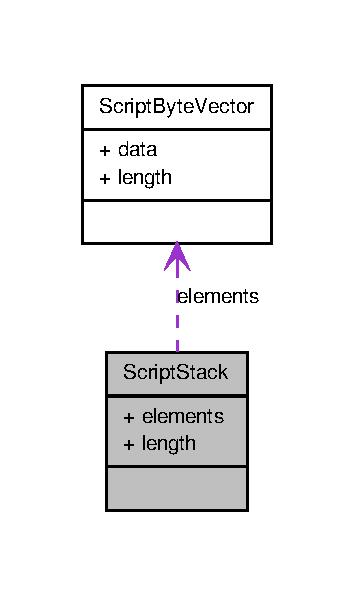
\includegraphics[width=170pt]{struct_script_stack__coll__graph}
\end{center}
\end{figure}
\subsection*{Data Fields}
\begin{DoxyCompactItemize}
\item 
struct \hyperlink{struct_script_byte_vector}{ScriptByteVector} $\ast$ \hyperlink{struct_script_stack_a39919a8f614861eedc5579d2bf18209a}{elements}
\item 
uint16\_\-t \hyperlink{struct_script_stack_a1892eba2086d12ac2b09005aeb09ea3b}{length}
\end{DoxyCompactItemize}


\subsection{Detailed Description}
Structure that holds byte vector data in a stack. 

Definition at line 33 of file Script.h.



\subsection{Field Documentation}
\hypertarget{struct_script_stack_a39919a8f614861eedc5579d2bf18209a}{
\index{ScriptStack@{ScriptStack}!elements@{elements}}
\index{elements@{elements}!ScriptStack@{ScriptStack}}
\subsubsection[{elements}]{\setlength{\rightskip}{0pt plus 5cm}struct {\bf ScriptByteVector}$\ast$ {\bf elements}}}
\label{struct_script_stack_a39919a8f614861eedc5579d2bf18209a}
Elements in the stack 

Definition at line 34 of file Script.h.

\hypertarget{struct_script_stack_a1892eba2086d12ac2b09005aeb09ea3b}{
\index{ScriptStack@{ScriptStack}!length@{length}}
\index{length@{length}!ScriptStack@{ScriptStack}}
\subsubsection[{length}]{\setlength{\rightskip}{0pt plus 5cm}uint16\_\-t {\bf length}}}
\label{struct_script_stack_a1892eba2086d12ac2b09005aeb09ea3b}
Length of the stack 

Definition at line 35 of file Script.h.



The documentation for this struct was generated from the following file:\begin{DoxyCompactItemize}
\item 
src/Object/\hyperlink{_script_8h}{Script.h}\end{DoxyCompactItemize}

\hypertarget{struct_shared_data}{
\section{SharedData Struct Reference}
\label{struct_shared_data}\index{SharedData@{SharedData}}
}


Stores byte data that can be shared amongst many ByteArrays.  




{\ttfamily \#include $<$ByteArray.h$>$}

\subsection*{Data Fields}
\begin{DoxyCompactItemize}
\item 
uint8\_\-t $\ast$ \hyperlink{struct_shared_data_abe222f6d3581e7920dcad5306cc906a8}{data}
\item 
uint32\_\-t \hyperlink{struct_shared_data_ad83c3d5d3f46e6278a77cb80eb2a0705}{referenceCount}
\end{DoxyCompactItemize}


\subsection{Detailed Description}
Stores byte data that can be shared amongst many ByteArrays. 

Definition at line 21 of file ByteArray.h.



\subsection{Field Documentation}
\hypertarget{struct_shared_data_abe222f6d3581e7920dcad5306cc906a8}{
\index{SharedData@{SharedData}!data@{data}}
\index{data@{data}!SharedData@{SharedData}}
\subsubsection[{data}]{\setlength{\rightskip}{0pt plus 5cm}uint8\_\-t$\ast$ {\bf data}}}
\label{struct_shared_data_abe222f6d3581e7920dcad5306cc906a8}
Pointer to byte data 

Definition at line 22 of file ByteArray.h.

\hypertarget{struct_shared_data_ad83c3d5d3f46e6278a77cb80eb2a0705}{
\index{SharedData@{SharedData}!referenceCount@{referenceCount}}
\index{referenceCount@{referenceCount}!SharedData@{SharedData}}
\subsubsection[{referenceCount}]{\setlength{\rightskip}{0pt plus 5cm}uint32\_\-t {\bf referenceCount}}}
\label{struct_shared_data_ad83c3d5d3f46e6278a77cb80eb2a0705}
References to this data 

Definition at line 23 of file ByteArray.h.



The documentation for this struct was generated from the following file:\begin{DoxyCompactItemize}
\item 
src/Object/\hyperlink{_byte_array_8h}{ByteArray.h}\end{DoxyCompactItemize}

\hypertarget{struct_transaction}{
\section{Transaction Struct Reference}
\label{struct_transaction}\index{Transaction@{Transaction}}
}


{\ttfamily \#include $<$Transaction.h$>$}



Collaboration diagram for Transaction:\nopagebreak
\begin{figure}[H]
\begin{center}
\leavevmode
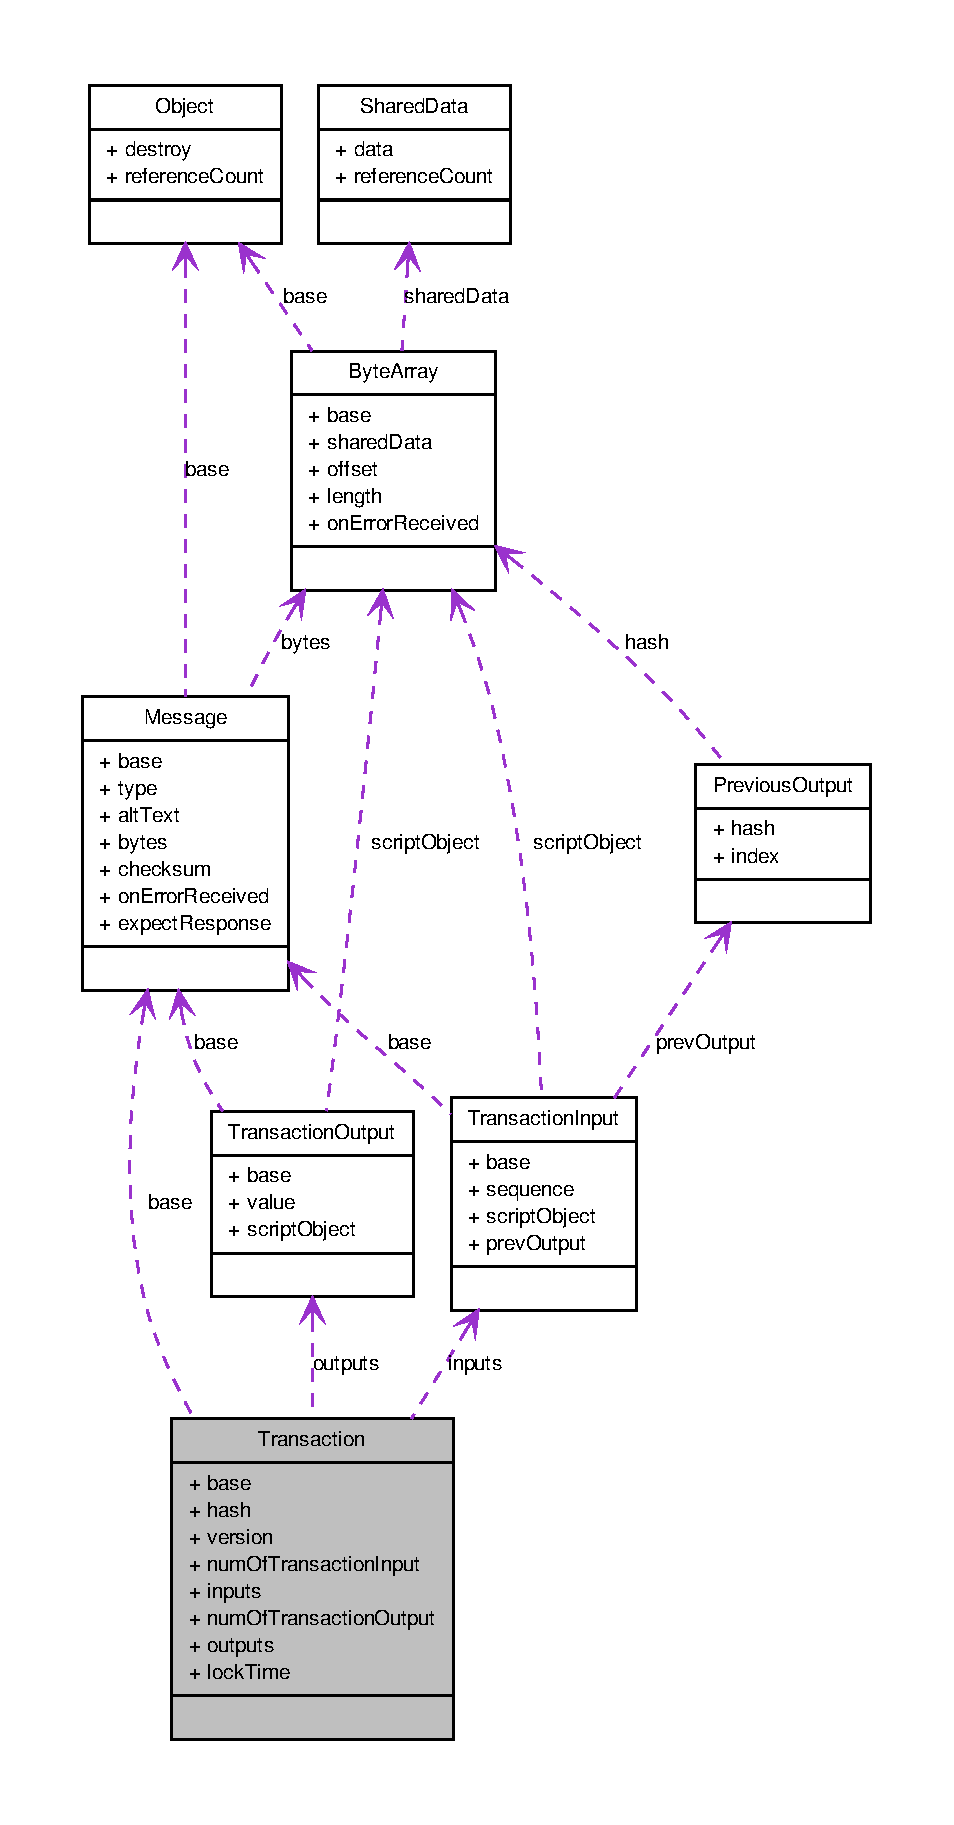
\includegraphics[height=600pt]{struct_transaction__coll__graph}
\end{center}
\end{figure}
\subsection*{Data Fields}
\begin{DoxyCompactItemize}
\item 
\hyperlink{struct_message}{Message} \hyperlink{struct_transaction_a8987f797adf70c3e174fd64cc68bc933}{base}
\item 
uint8\_\-t \hyperlink{struct_transaction_a7ff9da008bf055da1f1ba994c562057d}{hash} \mbox{[}32\mbox{]}
\item 
uint32\_\-t \hyperlink{struct_transaction_acd99bb05ca015e7d74448acb1deba7ca}{version}
\item 
uint32\_\-t \hyperlink{struct_transaction_ab67f7dee599d2ca5988caa53883a44ed}{numOfTransactionInput}
\item 
\hyperlink{struct_transaction_input}{TransactionInput} $\ast$$\ast$ \hyperlink{struct_transaction_a00cc03d624a6aef1bfeadcbe9dcde0fe}{inputs}
\item 
uint32\_\-t \hyperlink{struct_transaction_aeeae027bddb846b239fd05e203c0c62a}{numOfTransactionOutput}
\item 
\hyperlink{struct_transaction_output}{TransactionOutput} $\ast$$\ast$ \hyperlink{struct_transaction_a0f4d7ecc12680c61da7267851e819cf0}{outputs}
\item 
uint32\_\-t \hyperlink{struct_transaction_aea4d95211b00c311b2d84c6177429162}{lockTime}
\end{DoxyCompactItemize}


\subsection{Detailed Description}


Definition at line 28 of file Transaction.h.



\subsection{Field Documentation}
\hypertarget{struct_transaction_a8987f797adf70c3e174fd64cc68bc933}{
\index{Transaction@{Transaction}!base@{base}}
\index{base@{base}!Transaction@{Transaction}}
\subsubsection[{base}]{\setlength{\rightskip}{0pt plus 5cm}{\bf Message} {\bf base}}}
\label{struct_transaction_a8987f797adf70c3e174fd64cc68bc933}
\hyperlink{struct_message}{Message} base structure$>$ 

Definition at line 29 of file Transaction.h.

\hypertarget{struct_transaction_a7ff9da008bf055da1f1ba994c562057d}{
\index{Transaction@{Transaction}!hash@{hash}}
\index{hash@{hash}!Transaction@{Transaction}}
\subsubsection[{hash}]{\setlength{\rightskip}{0pt plus 5cm}uint8\_\-t {\bf hash}\mbox{[}32\mbox{]}}}
\label{struct_transaction_a7ff9da008bf055da1f1ba994c562057d}
The hash for this transaction. Null by default 

Definition at line 30 of file Transaction.h.

\hypertarget{struct_transaction_a00cc03d624a6aef1bfeadcbe9dcde0fe}{
\index{Transaction@{Transaction}!inputs@{inputs}}
\index{inputs@{inputs}!Transaction@{Transaction}}
\subsubsection[{inputs}]{\setlength{\rightskip}{0pt plus 5cm}{\bf TransactionInput}$\ast$$\ast$ {\bf inputs}}}
\label{struct_transaction_a00cc03d624a6aef1bfeadcbe9dcde0fe}
\hyperlink{struct_transaction_input}{TransactionInput} base structure 

Definition at line 33 of file Transaction.h.

\hypertarget{struct_transaction_aea4d95211b00c311b2d84c6177429162}{
\index{Transaction@{Transaction}!lockTime@{lockTime}}
\index{lockTime@{lockTime}!Transaction@{Transaction}}
\subsubsection[{lockTime}]{\setlength{\rightskip}{0pt plus 5cm}uint32\_\-t {\bf lockTime}}}
\label{struct_transaction_aea4d95211b00c311b2d84c6177429162}
The block number or timestamp at which this transaction is locked; A non-\/locked transaction must not be included in blocks. 

Definition at line 36 of file Transaction.h.

\hypertarget{struct_transaction_ab67f7dee599d2ca5988caa53883a44ed}{
\index{Transaction@{Transaction}!numOfTransactionInput@{numOfTransactionInput}}
\index{numOfTransactionInput@{numOfTransactionInput}!Transaction@{Transaction}}
\subsubsection[{numOfTransactionInput}]{\setlength{\rightskip}{0pt plus 5cm}uint32\_\-t {\bf numOfTransactionInput}}}
\label{struct_transaction_ab67f7dee599d2ca5988caa53883a44ed}
Number of TransactionInputs. How many inputs are already added to the transaction 

Definition at line 32 of file Transaction.h.

\hypertarget{struct_transaction_aeeae027bddb846b239fd05e203c0c62a}{
\index{Transaction@{Transaction}!numOfTransactionOutput@{numOfTransactionOutput}}
\index{numOfTransactionOutput@{numOfTransactionOutput}!Transaction@{Transaction}}
\subsubsection[{numOfTransactionOutput}]{\setlength{\rightskip}{0pt plus 5cm}uint32\_\-t {\bf numOfTransactionOutput}}}
\label{struct_transaction_aeeae027bddb846b239fd05e203c0c62a}
Number of TransactionOutputs. How many outputs are already added to the transaction 

Definition at line 34 of file Transaction.h.

\hypertarget{struct_transaction_a0f4d7ecc12680c61da7267851e819cf0}{
\index{Transaction@{Transaction}!outputs@{outputs}}
\index{outputs@{outputs}!Transaction@{Transaction}}
\subsubsection[{outputs}]{\setlength{\rightskip}{0pt plus 5cm}{\bf TransactionOutput}$\ast$$\ast$ {\bf outputs}}}
\label{struct_transaction_a0f4d7ecc12680c61da7267851e819cf0}
\hyperlink{struct_transaction_output}{TransactionOutput} base structure 

Definition at line 35 of file Transaction.h.

\hypertarget{struct_transaction_acd99bb05ca015e7d74448acb1deba7ca}{
\index{Transaction@{Transaction}!version@{version}}
\index{version@{version}!Transaction@{Transaction}}
\subsubsection[{version}]{\setlength{\rightskip}{0pt plus 5cm}uint32\_\-t {\bf version}}}
\label{struct_transaction_acd99bb05ca015e7d74448acb1deba7ca}
Version of the transaction data format. 1 by default 

Definition at line 31 of file Transaction.h.



The documentation for this struct was generated from the following file:\begin{DoxyCompactItemize}
\item 
src/Object/Message/\hyperlink{_transaction_8h}{Transaction.h}\end{DoxyCompactItemize}

\hypertarget{struct_transaction_input}{
\section{TransactionInput Struct Reference}
\label{struct_transaction_input}\index{TransactionInput@{TransactionInput}}
}


contains \hyperlink{struct_previous_output}{PreviousOutput} structure and Example of the structure: \{ prev\_\-out: \{ hash: \char`\"{}0000000000000000000000000000000000000000000000000000000000000000\char`\"{}, n: 4294967295 \}, coinbase: \char`\"{}044c86041b0152\char`\"{} \}  




{\ttfamily \#include $<$TransactionInput.h$>$}



Collaboration diagram for TransactionInput:\nopagebreak
\begin{figure}[H]
\begin{center}
\leavevmode
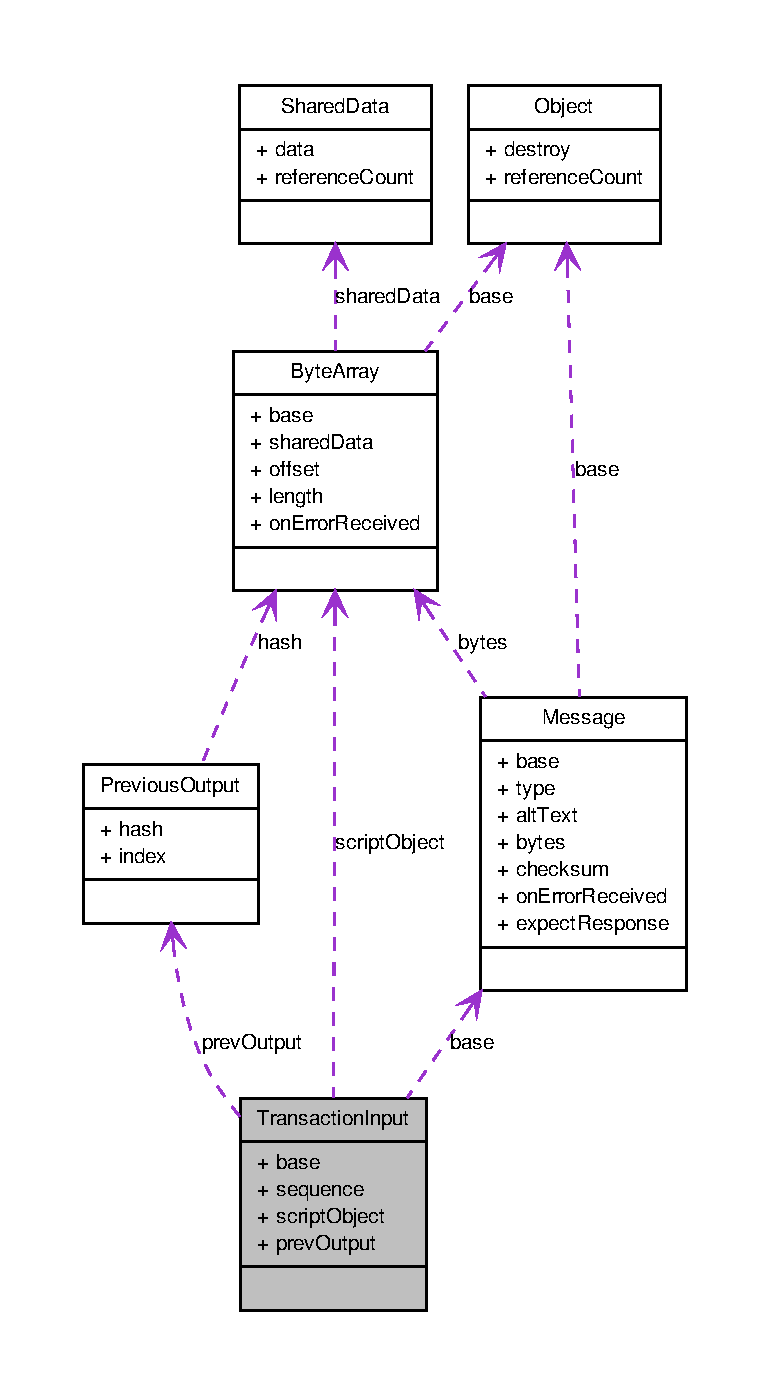
\includegraphics[height=600pt]{struct_transaction_input__coll__graph}
\end{center}
\end{figure}
\subsection*{Data Fields}
\begin{DoxyCompactItemize}
\item 
\hyperlink{struct_message}{Message} \hyperlink{struct_transaction_input_a8987f797adf70c3e174fd64cc68bc933}{base}
\item 
uint32\_\-t \hyperlink{struct_transaction_input_a0ab03ef2cc38198d3666a992a245fddf}{sequence}
\item 
\hyperlink{struct_byte_array}{Script} $\ast$ \hyperlink{struct_transaction_input_ac420de2766b1358b5e325cfc21a76aa3}{scriptObject}
\item 
\hyperlink{struct_previous_output}{PreviousOutput} \hyperlink{struct_transaction_input_a20cfe78368fb9825302ce5cdb076f8b1}{prevOutput}
\end{DoxyCompactItemize}


\subsection{Detailed Description}
contains \hyperlink{struct_previous_output}{PreviousOutput} structure and Example of the structure: \{ prev\_\-out: \{ hash: \char`\"{}0000000000000000000000000000000000000000000000000000000000000000\char`\"{}, n: 4294967295 \}, coinbase: \char`\"{}044c86041b0152\char`\"{} \} 

that handles input in transactions 

Definition at line 51 of file TransactionInput.h.



\subsection{Field Documentation}
\hypertarget{struct_transaction_input_a8987f797adf70c3e174fd64cc68bc933}{
\index{TransactionInput@{TransactionInput}!base@{base}}
\index{base@{base}!TransactionInput@{TransactionInput}}
\subsubsection[{base}]{\setlength{\rightskip}{0pt plus 5cm}{\bf Message} {\bf base}}}
\label{struct_transaction_input_a8987f797adf70c3e174fd64cc68bc933}
\hyperlink{struct_message}{Message} base structure 

Definition at line 52 of file TransactionInput.h.

\hypertarget{struct_transaction_input_a20cfe78368fb9825302ce5cdb076f8b1}{
\index{TransactionInput@{TransactionInput}!prevOutput@{prevOutput}}
\index{prevOutput@{prevOutput}!TransactionInput@{TransactionInput}}
\subsubsection[{prevOutput}]{\setlength{\rightskip}{0pt plus 5cm}{\bf PreviousOutput} {\bf prevOutput}}}
\label{struct_transaction_input_a20cfe78368fb9825302ce5cdb076f8b1}
A locator for a previous output being spent. 

Definition at line 55 of file TransactionInput.h.

\hypertarget{struct_transaction_input_ac420de2766b1358b5e325cfc21a76aa3}{
\index{TransactionInput@{TransactionInput}!scriptObject@{scriptObject}}
\index{scriptObject@{scriptObject}!TransactionInput@{TransactionInput}}
\subsubsection[{scriptObject}]{\setlength{\rightskip}{0pt plus 5cm}{\bf Script}$\ast$ {\bf scriptObject}}}
\label{struct_transaction_input_ac420de2766b1358b5e325cfc21a76aa3}
Contains script information as a Script. 

Definition at line 54 of file TransactionInput.h.

\hypertarget{struct_transaction_input_a0ab03ef2cc38198d3666a992a245fddf}{
\index{TransactionInput@{TransactionInput}!sequence@{sequence}}
\index{sequence@{sequence}!TransactionInput@{TransactionInput}}
\subsubsection[{sequence}]{\setlength{\rightskip}{0pt plus 5cm}uint32\_\-t {\bf sequence}}}
\label{struct_transaction_input_a0ab03ef2cc38198d3666a992a245fddf}
The version of this transaction input. Not used in protocol v0.3.18.00. Set to 0 for transactions that may someday be open to change after broadcast, set to \_\-TRANSACTION\_\-INPUT\_\-FINAL if this input never needs to be changed after broadcast. 

Definition at line 53 of file TransactionInput.h.



The documentation for this struct was generated from the following file:\begin{DoxyCompactItemize}
\item 
src/Object/Message/\hyperlink{_transaction_input_8h}{TransactionInput.h}\end{DoxyCompactItemize}

\hypertarget{struct_transaction_output}{
\section{TransactionOutput Struct Reference}
\label{struct_transaction_output}\index{TransactionOutput@{TransactionOutput}}
}


{\ttfamily \#include $<$TransactionOutput.h$>$}



Collaboration diagram for TransactionOutput:\nopagebreak
\begin{figure}[H]
\begin{center}
\leavevmode
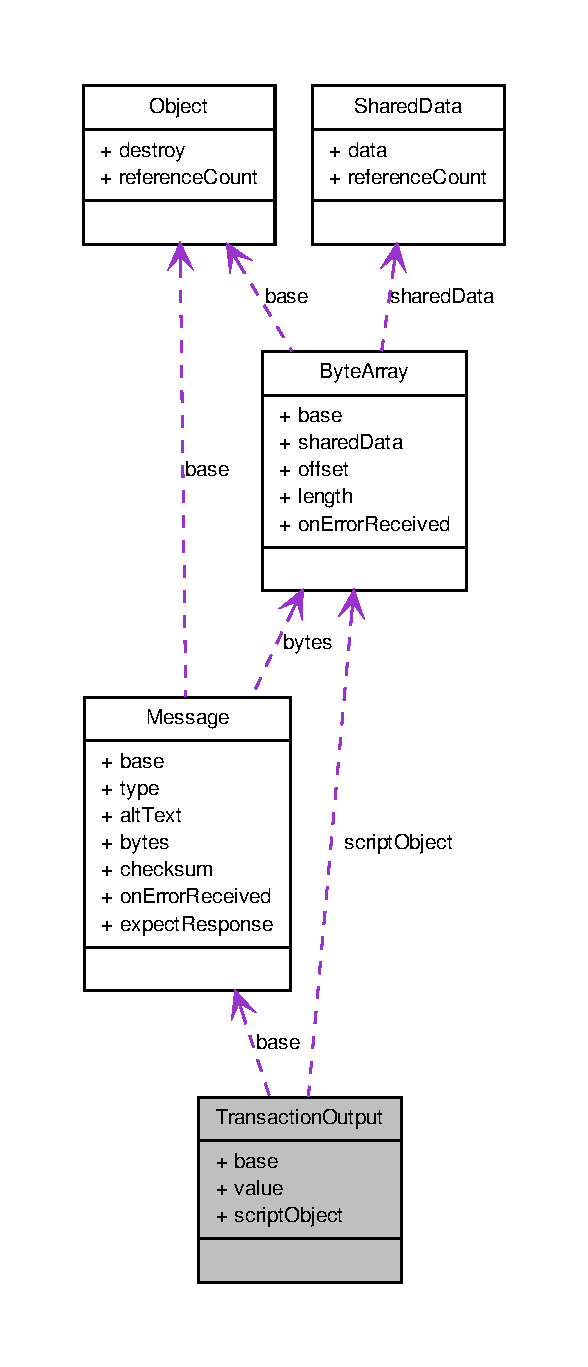
\includegraphics[height=600pt]{struct_transaction_output__coll__graph}
\end{center}
\end{figure}
\subsection*{Data Fields}
\begin{DoxyCompactItemize}
\item 
\hyperlink{struct_message}{Message} \hyperlink{struct_transaction_output_a8987f797adf70c3e174fd64cc68bc933}{base}
\item 
uint64\_\-t \hyperlink{struct_transaction_output_a4e630859cc0e2a22bd6acf39a6a8e218}{value}
\item 
\hyperlink{struct_byte_array}{Script} $\ast$ \hyperlink{struct_transaction_output_ac420de2766b1358b5e325cfc21a76aa3}{scriptObject}
\end{DoxyCompactItemize}


\subsection{Detailed Description}


Definition at line 17 of file TransactionOutput.h.



\subsection{Field Documentation}
\hypertarget{struct_transaction_output_a8987f797adf70c3e174fd64cc68bc933}{
\index{TransactionOutput@{TransactionOutput}!base@{base}}
\index{base@{base}!TransactionOutput@{TransactionOutput}}
\subsubsection[{base}]{\setlength{\rightskip}{0pt plus 5cm}{\bf Message} {\bf base}}}
\label{struct_transaction_output_a8987f797adf70c3e174fd64cc68bc933}
\hyperlink{struct_message}{Message} base structure 

Definition at line 18 of file TransactionOutput.h.

\hypertarget{struct_transaction_output_ac420de2766b1358b5e325cfc21a76aa3}{
\index{TransactionOutput@{TransactionOutput}!scriptObject@{scriptObject}}
\index{scriptObject@{scriptObject}!TransactionOutput@{TransactionOutput}}
\subsubsection[{scriptObject}]{\setlength{\rightskip}{0pt plus 5cm}{\bf Script}$\ast$ {\bf scriptObject}}}
\label{struct_transaction_output_ac420de2766b1358b5e325cfc21a76aa3}
The output script object 

Definition at line 20 of file TransactionOutput.h.

\hypertarget{struct_transaction_output_a4e630859cc0e2a22bd6acf39a6a8e218}{
\index{TransactionOutput@{TransactionOutput}!value@{value}}
\index{value@{value}!TransactionOutput@{TransactionOutput}}
\subsubsection[{value}]{\setlength{\rightskip}{0pt plus 5cm}uint64\_\-t {\bf value}}}
\label{struct_transaction_output_a4e630859cc0e2a22bd6acf39a6a8e218}
The transaction value 

Definition at line 19 of file TransactionOutput.h.



The documentation for this struct was generated from the following file:\begin{DoxyCompactItemize}
\item 
src/Object/Message/\hyperlink{_transaction_output_8h}{TransactionOutput.h}\end{DoxyCompactItemize}

\hypertarget{struct_tranx_in}{
\section{TranxIn Struct Reference}
\label{struct_tranx_in}\index{TranxIn@{TranxIn}}
}


{\ttfamily \#include $<$Commands.h$>$}



Collaboration diagram for TranxIn:\nopagebreak
\begin{figure}[H]
\begin{center}
\leavevmode
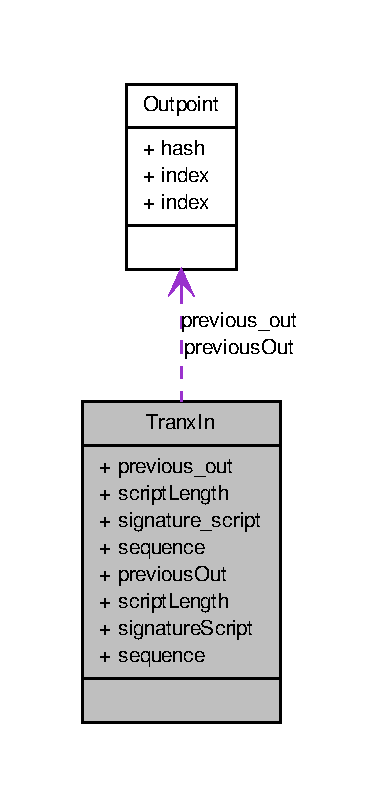
\includegraphics[width=183pt]{struct_tranx_in__coll__graph}
\end{center}
\end{figure}
\subsection*{Data Fields}
\begin{DoxyCompactItemize}
\item 
struct \hyperlink{struct_outpoint}{Outpoint} $\ast$ \hyperlink{struct_tranx_in_a694240f5463d28f9cb6cb2f8de4a5a45}{previous\_\-out}
\item 
uint32\_\-t \hyperlink{struct_tranx_in_a756d651ccdd4c06f59685e337cf2e840}{scriptLength}
\item 
unsigned char \hyperlink{struct_tranx_in_acd5b457285f7e816fbb23777406a701a}{signature\_\-script} \mbox{[}$\,$\mbox{]}
\item 
uint32\_\-t \hyperlink{struct_tranx_in_a0ab03ef2cc38198d3666a992a245fddf}{sequence}
\item 
struct \hyperlink{struct_outpoint}{Outpoint} \hyperlink{struct_tranx_in_a2889e84785c9df5cba88abaaa03eb206}{previousOut}
\item 
unsigned int \hyperlink{struct_tranx_in_a00601157399e1c73bddee66c716926f4}{scriptLength}
\item 
unsigned char $\ast$ \hyperlink{struct_tranx_in_a3d518a810ef5d47feb63829a61ced9e1}{signatureScript}
\item 
unsigned int \hyperlink{struct_tranx_in_a18ec6560d3738f9c1bc8ed50f2e570c1}{sequence}
\end{DoxyCompactItemize}


\subsection{Detailed Description}


Definition at line 35 of file Commands.h.



\subsection{Field Documentation}
\hypertarget{struct_tranx_in_a694240f5463d28f9cb6cb2f8de4a5a45}{
\index{TranxIn@{TranxIn}!previous\_\-out@{previous\_\-out}}
\index{previous\_\-out@{previous\_\-out}!TranxIn@{TranxIn}}
\subsubsection[{previous\_\-out}]{\setlength{\rightskip}{0pt plus 5cm}struct {\bf Outpoint}$\ast$ {\bf previous\_\-out}}}
\label{struct_tranx_in_a694240f5463d28f9cb6cb2f8de4a5a45}


Definition at line 36 of file Commands.h.

\hypertarget{struct_tranx_in_a2889e84785c9df5cba88abaaa03eb206}{
\index{TranxIn@{TranxIn}!previousOut@{previousOut}}
\index{previousOut@{previousOut}!TranxIn@{TranxIn}}
\subsubsection[{previousOut}]{\setlength{\rightskip}{0pt plus 5cm}struct {\bf Outpoint} {\bf previousOut}}}
\label{struct_tranx_in_a2889e84785c9df5cba88abaaa03eb206}


Definition at line 154 of file Protocol.h.

\hypertarget{struct_tranx_in_a756d651ccdd4c06f59685e337cf2e840}{
\index{TranxIn@{TranxIn}!scriptLength@{scriptLength}}
\index{scriptLength@{scriptLength}!TranxIn@{TranxIn}}
\subsubsection[{scriptLength}]{\setlength{\rightskip}{0pt plus 5cm}uint32\_\-t {\bf scriptLength}}}
\label{struct_tranx_in_a756d651ccdd4c06f59685e337cf2e840}


Definition at line 37 of file Commands.h.

\hypertarget{struct_tranx_in_a00601157399e1c73bddee66c716926f4}{
\index{TranxIn@{TranxIn}!scriptLength@{scriptLength}}
\index{scriptLength@{scriptLength}!TranxIn@{TranxIn}}
\subsubsection[{scriptLength}]{\setlength{\rightskip}{0pt plus 5cm}unsigned int {\bf scriptLength}}}
\label{struct_tranx_in_a00601157399e1c73bddee66c716926f4}


Definition at line 155 of file Protocol.h.

\hypertarget{struct_tranx_in_a18ec6560d3738f9c1bc8ed50f2e570c1}{
\index{TranxIn@{TranxIn}!sequence@{sequence}}
\index{sequence@{sequence}!TranxIn@{TranxIn}}
\subsubsection[{sequence}]{\setlength{\rightskip}{0pt plus 5cm}unsigned int {\bf sequence}}}
\label{struct_tranx_in_a18ec6560d3738f9c1bc8ed50f2e570c1}


Definition at line 157 of file Protocol.h.

\hypertarget{struct_tranx_in_a0ab03ef2cc38198d3666a992a245fddf}{
\index{TranxIn@{TranxIn}!sequence@{sequence}}
\index{sequence@{sequence}!TranxIn@{TranxIn}}
\subsubsection[{sequence}]{\setlength{\rightskip}{0pt plus 5cm}uint32\_\-t {\bf sequence}}}
\label{struct_tranx_in_a0ab03ef2cc38198d3666a992a245fddf}


Definition at line 39 of file Commands.h.

\hypertarget{struct_tranx_in_acd5b457285f7e816fbb23777406a701a}{
\index{TranxIn@{TranxIn}!signature\_\-script@{signature\_\-script}}
\index{signature\_\-script@{signature\_\-script}!TranxIn@{TranxIn}}
\subsubsection[{signature\_\-script}]{\setlength{\rightskip}{0pt plus 5cm}unsigned char {\bf signature\_\-script}\mbox{[}$\,$\mbox{]}}}
\label{struct_tranx_in_acd5b457285f7e816fbb23777406a701a}


Definition at line 38 of file Commands.h.

\hypertarget{struct_tranx_in_a3d518a810ef5d47feb63829a61ced9e1}{
\index{TranxIn@{TranxIn}!signatureScript@{signatureScript}}
\index{signatureScript@{signatureScript}!TranxIn@{TranxIn}}
\subsubsection[{signatureScript}]{\setlength{\rightskip}{0pt plus 5cm}unsigned char$\ast$ {\bf signatureScript}}}
\label{struct_tranx_in_a3d518a810ef5d47feb63829a61ced9e1}


Definition at line 156 of file Protocol.h.



The documentation for this struct was generated from the following files:\begin{DoxyCompactItemize}
\item 
src/Object/NetworkProtocol/\hyperlink{_commands_8h}{Commands.h}\item 
src/Object/NetworkProtocol/\hyperlink{_protocol_8h}{Protocol.h}\end{DoxyCompactItemize}

\hypertarget{struct_tranx_out}{
\section{TranxOut Struct Reference}
\label{struct_tranx_out}\index{TranxOut@{TranxOut}}
}


{\ttfamily \#include $<$Commands.h$>$}

\subsection*{Data Fields}
\begin{DoxyCompactItemize}
\item 
uint64\_\-t \hyperlink{struct_tranx_out_a4e630859cc0e2a22bd6acf39a6a8e218}{value}
\item 
uint32\_\-t \hyperlink{struct_tranx_out_a895859eb7d18cd9b6cb38c25ced2418e}{pkScriptLength}
\item 
unsigned char \hyperlink{struct_tranx_out_a57661961e62f14ddb90c75c2c130b041}{pkScript} \mbox{[}$\,$\mbox{]}
\item 
unsigned int \hyperlink{struct_tranx_out_a2a5a27690c40c531d0a8385dc4f66a95}{value}
\item 
unsigned int \hyperlink{struct_tranx_out_a12d43c2eb75d61a2698e5c78f2f6122c}{pkScriptLength}
\item 
unsigned char $\ast$ \hyperlink{struct_tranx_out_a1065be8e3e985afe6b60c410ca157d61}{pkScript}
\end{DoxyCompactItemize}


\subsection{Detailed Description}


Definition at line 48 of file Commands.h.



\subsection{Field Documentation}
\hypertarget{struct_tranx_out_a57661961e62f14ddb90c75c2c130b041}{
\index{TranxOut@{TranxOut}!pkScript@{pkScript}}
\index{pkScript@{pkScript}!TranxOut@{TranxOut}}
\subsubsection[{pkScript}]{\setlength{\rightskip}{0pt plus 5cm}unsigned char {\bf pkScript}\mbox{[}$\,$\mbox{]}}}
\label{struct_tranx_out_a57661961e62f14ddb90c75c2c130b041}


Definition at line 51 of file Commands.h.

\hypertarget{struct_tranx_out_a1065be8e3e985afe6b60c410ca157d61}{
\index{TranxOut@{TranxOut}!pkScript@{pkScript}}
\index{pkScript@{pkScript}!TranxOut@{TranxOut}}
\subsubsection[{pkScript}]{\setlength{\rightskip}{0pt plus 5cm}unsigned char$\ast$ {\bf pkScript}}}
\label{struct_tranx_out_a1065be8e3e985afe6b60c410ca157d61}


Definition at line 166 of file Protocol.h.

\hypertarget{struct_tranx_out_a12d43c2eb75d61a2698e5c78f2f6122c}{
\index{TranxOut@{TranxOut}!pkScriptLength@{pkScriptLength}}
\index{pkScriptLength@{pkScriptLength}!TranxOut@{TranxOut}}
\subsubsection[{pkScriptLength}]{\setlength{\rightskip}{0pt plus 5cm}unsigned int {\bf pkScriptLength}}}
\label{struct_tranx_out_a12d43c2eb75d61a2698e5c78f2f6122c}


Definition at line 165 of file Protocol.h.

\hypertarget{struct_tranx_out_a895859eb7d18cd9b6cb38c25ced2418e}{
\index{TranxOut@{TranxOut}!pkScriptLength@{pkScriptLength}}
\index{pkScriptLength@{pkScriptLength}!TranxOut@{TranxOut}}
\subsubsection[{pkScriptLength}]{\setlength{\rightskip}{0pt plus 5cm}uint32\_\-t {\bf pkScriptLength}}}
\label{struct_tranx_out_a895859eb7d18cd9b6cb38c25ced2418e}


Definition at line 50 of file Commands.h.

\hypertarget{struct_tranx_out_a2a5a27690c40c531d0a8385dc4f66a95}{
\index{TranxOut@{TranxOut}!value@{value}}
\index{value@{value}!TranxOut@{TranxOut}}
\subsubsection[{value}]{\setlength{\rightskip}{0pt plus 5cm}unsigned int {\bf value}}}
\label{struct_tranx_out_a2a5a27690c40c531d0a8385dc4f66a95}


Definition at line 164 of file Protocol.h.

\hypertarget{struct_tranx_out_a4e630859cc0e2a22bd6acf39a6a8e218}{
\index{TranxOut@{TranxOut}!value@{value}}
\index{value@{value}!TranxOut@{TranxOut}}
\subsubsection[{value}]{\setlength{\rightskip}{0pt plus 5cm}uint64\_\-t {\bf value}}}
\label{struct_tranx_out_a4e630859cc0e2a22bd6acf39a6a8e218}


Definition at line 49 of file Commands.h.



The documentation for this struct was generated from the following files:\begin{DoxyCompactItemize}
\item 
src/Object/NetworkProtocol/\hyperlink{_commands_8h}{Commands.h}\item 
src/Object/NetworkProtocol/\hyperlink{_protocol_8h}{Protocol.h}\end{DoxyCompactItemize}

\hypertarget{struct_var_len_int}{
\section{VarLenInt Struct Reference}
\label{struct_var_len_int}\index{VarLenInt@{VarLenInt}}
}


Variable length integer specified in Bitcoin protocol.  




{\ttfamily \#include $<$VarLenInt.h$>$}

\subsection*{Data Fields}
\begin{DoxyCompactItemize}
\item 
uint64\_\-t \hyperlink{struct_var_len_int_a4e630859cc0e2a22bd6acf39a6a8e218}{value}
\item 
uint8\_\-t \hyperlink{struct_var_len_int_af922c72fe1d5915971491918ff5f923e}{storageSize}
\end{DoxyCompactItemize}


\subsection{Detailed Description}
Variable length integer specified in Bitcoin protocol. 

Contains decoded variable size integer information. \begin{DoxySeeAlso}{See also}
\hyperlink{_var_len_int_8h}{VarLenInt.h} 
\end{DoxySeeAlso}


Definition at line 26 of file VarLenInt.h.



\subsection{Field Documentation}
\hypertarget{struct_var_len_int_af922c72fe1d5915971491918ff5f923e}{
\index{VarLenInt@{VarLenInt}!storageSize@{storageSize}}
\index{storageSize@{storageSize}!VarLenInt@{VarLenInt}}
\subsubsection[{storageSize}]{\setlength{\rightskip}{0pt plus 5cm}uint8\_\-t {\bf storageSize}}}
\label{struct_var_len_int_af922c72fe1d5915971491918ff5f923e}
Size of the integer when encoded in bytes 

Definition at line 28 of file VarLenInt.h.

\hypertarget{struct_var_len_int_a4e630859cc0e2a22bd6acf39a6a8e218}{
\index{VarLenInt@{VarLenInt}!value@{value}}
\index{value@{value}!VarLenInt@{VarLenInt}}
\subsubsection[{value}]{\setlength{\rightskip}{0pt plus 5cm}uint64\_\-t {\bf value}}}
\label{struct_var_len_int_a4e630859cc0e2a22bd6acf39a6a8e218}
Integer value 

Definition at line 27 of file VarLenInt.h.



The documentation for this struct was generated from the following file:\begin{DoxyCompactItemize}
\item 
src/Utils/VariableLengthInteger/\hyperlink{_var_len_int_8h}{VarLenInt.h}\end{DoxyCompactItemize}

\hypertarget{struct_version_checksum_bytes}{
\section{VersionChecksumBytes Struct Reference}
\label{struct_version_checksum_bytes}\index{VersionChecksumBytes@{VersionChecksumBytes}}
}


Structure for \hyperlink{struct_version_checksum_bytes}{VersionChecksumBytes} objects.  




{\ttfamily \#include $<$VersionChecksumBytes.h$>$}



Collaboration diagram for VersionChecksumBytes:\nopagebreak
\begin{figure}[H]
\begin{center}
\leavevmode
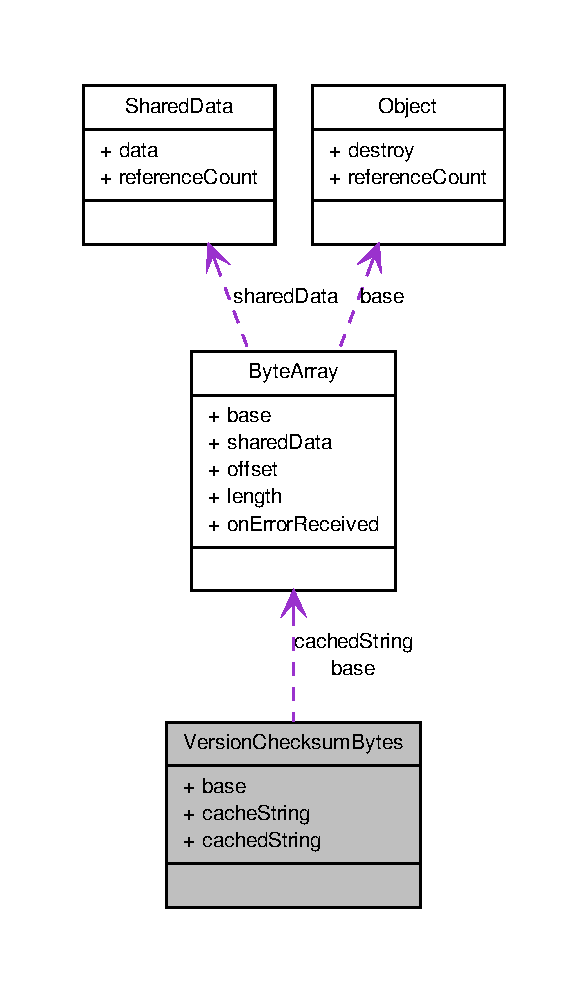
\includegraphics[width=282pt]{struct_version_checksum_bytes__coll__graph}
\end{center}
\end{figure}
\subsection*{Data Fields}
\begin{DoxyCompactItemize}
\item 
\hyperlink{struct_byte_array}{ByteArray} \hyperlink{struct_version_checksum_bytes_a403d3e7fd73c70aa24590627ed54844e}{base}
\item 
int \hyperlink{struct_version_checksum_bytes_a440754891ba48c34d0ec933efc36e050}{cacheString}
\item 
\hyperlink{struct_byte_array}{ByteArray} $\ast$ \hyperlink{struct_version_checksum_bytes_a25e4ea0f9f3ce1cce55f374afbba99c6}{cachedString}
\end{DoxyCompactItemize}


\subsection{Detailed Description}
Structure for \hyperlink{struct_version_checksum_bytes}{VersionChecksumBytes} objects. 

\begin{DoxySeeAlso}{See also}
\hyperlink{_version_checksum_bytes_8h}{VersionChecksumBytes.h} 
\end{DoxySeeAlso}


Definition at line 25 of file VersionChecksumBytes.h.



\subsection{Field Documentation}
\hypertarget{struct_version_checksum_bytes_a403d3e7fd73c70aa24590627ed54844e}{
\index{VersionChecksumBytes@{VersionChecksumBytes}!base@{base}}
\index{base@{base}!VersionChecksumBytes@{VersionChecksumBytes}}
\subsubsection[{base}]{\setlength{\rightskip}{0pt plus 5cm}{\bf ByteArray} {\bf base}}}
\label{struct_version_checksum_bytes_a403d3e7fd73c70aa24590627ed54844e}
\hyperlink{struct_byte_array}{ByteArray} base structure 

Definition at line 26 of file VersionChecksumBytes.h.

\hypertarget{struct_version_checksum_bytes_a25e4ea0f9f3ce1cce55f374afbba99c6}{
\index{VersionChecksumBytes@{VersionChecksumBytes}!cachedString@{cachedString}}
\index{cachedString@{cachedString}!VersionChecksumBytes@{VersionChecksumBytes}}
\subsubsection[{cachedString}]{\setlength{\rightskip}{0pt plus 5cm}{\bf ByteArray}$\ast$ {\bf cachedString}}}
\label{struct_version_checksum_bytes_a25e4ea0f9f3ce1cce55f374afbba99c6}
Pointer to cached \hyperlink{struct_byte_array}{ByteArray} string 

Definition at line 28 of file VersionChecksumBytes.h.

\hypertarget{struct_version_checksum_bytes_a440754891ba48c34d0ec933efc36e050}{
\index{VersionChecksumBytes@{VersionChecksumBytes}!cacheString@{cacheString}}
\index{cacheString@{cacheString}!VersionChecksumBytes@{VersionChecksumBytes}}
\subsubsection[{cacheString}]{\setlength{\rightskip}{0pt plus 5cm}int {\bf cacheString}}}
\label{struct_version_checksum_bytes_a440754891ba48c34d0ec933efc36e050}
If true, cache string 

Definition at line 27 of file VersionChecksumBytes.h.



The documentation for this struct was generated from the following file:\begin{DoxyCompactItemize}
\item 
src/Object/VersionChecksumBytes/\hyperlink{_version_checksum_bytes_8h}{VersionChecksumBytes.h}\end{DoxyCompactItemize}

\chapter{File Documentation}
\hypertarget{_base58_8c}{
\section{src/Base58/Base58.c File Reference}
\label{_base58_8c}\index{src/Base58/Base58.c@{src/Base58/Base58.c}}
}
{\ttfamily \#include \char`\"{}Base58.h\char`\"{}}\par
{\ttfamily \#include \char`\"{}../BigInt/BigInt.h\char`\"{}}\par
{\ttfamily \#include $<$stdint.h$>$}\par
Include dependency graph for Base58.c:\nopagebreak
\begin{figure}[H]
\begin{center}
\leavevmode
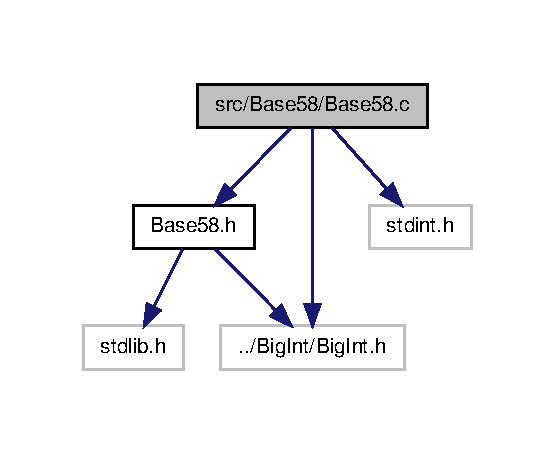
\includegraphics[width=266pt]{_base58_8c__incl}
\end{center}
\end{figure}
\subsection*{Functions}
\begin{DoxyCompactItemize}
\item 
\hyperlink{struct_big_int}{BigInt} \hyperlink{_base58_8c_a698fb6717b2cbd17d02ff52b09d84fe5}{DecodeBase58} (char $\ast$str)
\begin{DoxyCompactList}\small\item\em Decodes base 58 string into byte data as a \hyperlink{struct_big_int}{BigInt}. \end{DoxyCompactList}\item 
uint8\_\-t $\ast$ \hyperlink{_base58_8c_a638fbbbf6ac769d7ac1e730437fce0c0}{VerifyAndRemoveCheckSum} (uint8\_\-t $\ast$data)
\item 
\hyperlink{struct_big_int}{BigInt} \hyperlink{_base58_8c_a20b174879ad363a02444d6dfd0c3956f}{DecodeBase58Checked} (char $\ast$str, void($\ast$onErrorReceived)(\hyperlink{_constants_8h_a2c3e4bb40f36b262a5214e2da2bca9c5}{Error} error, char $\ast$,...))
\begin{DoxyCompactList}\small\item\em Decodes base 58 string into byte data as a \hyperlink{struct_big_int}{BigInt} and checks a 4 byte checksum. \end{DoxyCompactList}\item 
char $\ast$ \hyperlink{_base58_8c_a8eba0d420462df41d21fa7369a9cf2de}{EncodeBase58} (uint8\_\-t $\ast$bytes, uint8\_\-t len)
\begin{DoxyCompactList}\small\item\em Encodes byte data into base 58. \end{DoxyCompactList}\item 
uint8\_\-t $\ast$ \hyperlink{_base58_8c_a0e3eca914bcab6d9c960347ed24ca8d3}{GetCheckSum} (uint8\_\-t $\ast$data)
\end{DoxyCompactItemize}


\subsection{Function Documentation}
\hypertarget{_base58_8c_a698fb6717b2cbd17d02ff52b09d84fe5}{
\index{Base58.c@{Base58.c}!DecodeBase58@{DecodeBase58}}
\index{DecodeBase58@{DecodeBase58}!Base58.c@{Base58.c}}
\subsubsection[{DecodeBase58}]{\setlength{\rightskip}{0pt plus 5cm}{\bf BigInt} DecodeBase58 (
\begin{DoxyParamCaption}
\item[{char $\ast$}]{str}
\end{DoxyParamCaption}
)}}
\label{_base58_8c_a698fb6717b2cbd17d02ff52b09d84fe5}


Decodes base 58 string into byte data as a \hyperlink{struct_big_int}{BigInt}. 


\begin{DoxyParams}{Parameters}
{\em str} & Base 58 string to decode. \\
\hline
\end{DoxyParams}
\begin{DoxyReturn}{Returns}
Pointer to the byte data as a \hyperlink{struct_big_int}{BigInt}. The byte data will be created in this function. Remember to free the data. On error the big int will have a NULL data pointer. 
\end{DoxyReturn}


Definition at line 14 of file Base58.c.



Here is the call graph for this function:\nopagebreak
\begin{figure}[H]
\begin{center}
\leavevmode
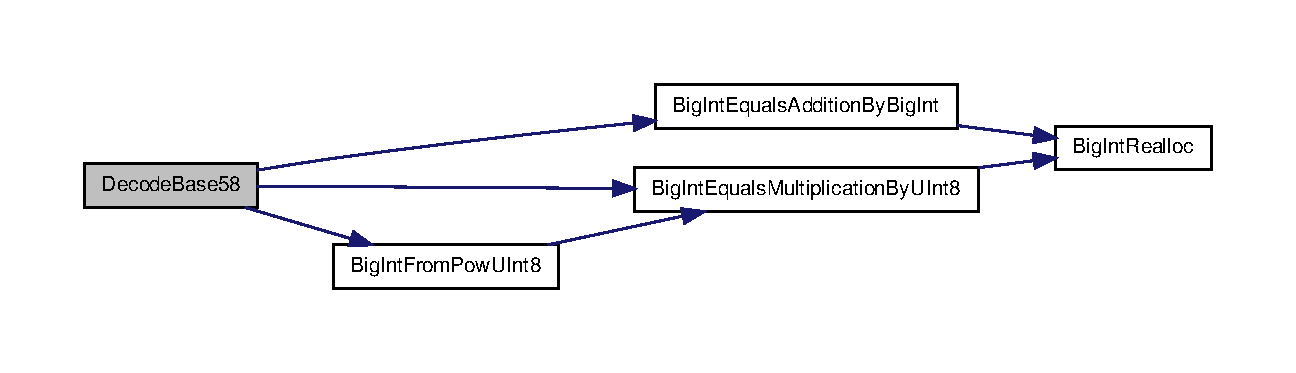
\includegraphics[width=400pt]{_base58_8c_a698fb6717b2cbd17d02ff52b09d84fe5_cgraph}
\end{center}
\end{figure}




Here is the caller graph for this function:\nopagebreak
\begin{figure}[H]
\begin{center}
\leavevmode
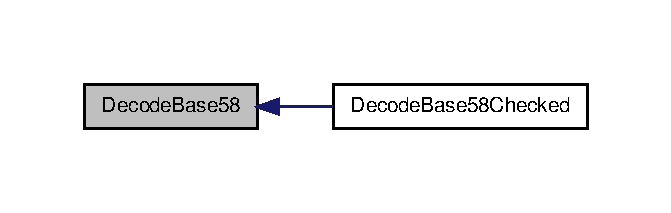
\includegraphics[width=322pt]{_base58_8c_a698fb6717b2cbd17d02ff52b09d84fe5_icgraph}
\end{center}
\end{figure}


\hypertarget{_base58_8c_a20b174879ad363a02444d6dfd0c3956f}{
\index{Base58.c@{Base58.c}!DecodeBase58Checked@{DecodeBase58Checked}}
\index{DecodeBase58Checked@{DecodeBase58Checked}!Base58.c@{Base58.c}}
\subsubsection[{DecodeBase58Checked}]{\setlength{\rightskip}{0pt plus 5cm}{\bf BigInt} DecodeBase58Checked (
\begin{DoxyParamCaption}
\item[{char $\ast$}]{str, }
\item[{void($\ast$)({\bf Error} error, char $\ast$,...)}]{onErrorReceived}
\end{DoxyParamCaption}
)}}
\label{_base58_8c_a20b174879ad363a02444d6dfd0c3956f}


Decodes base 58 string into byte data as a \hyperlink{struct_big_int}{BigInt} and checks a 4 byte checksum. 


\begin{DoxyParams}{Parameters}
{\em str} & Base 58 string to decode. \\
\hline
\end{DoxyParams}
\begin{DoxyReturn}{Returns}
Byte data as a \hyperlink{struct_big_int}{BigInt}. Is zero on failure. Checksum is included in returned data. On error the big int will have a NULL data pointer. 
\end{DoxyReturn}


Definition at line 128 of file Base58.c.



Here is the call graph for this function:\nopagebreak
\begin{figure}[H]
\begin{center}
\leavevmode
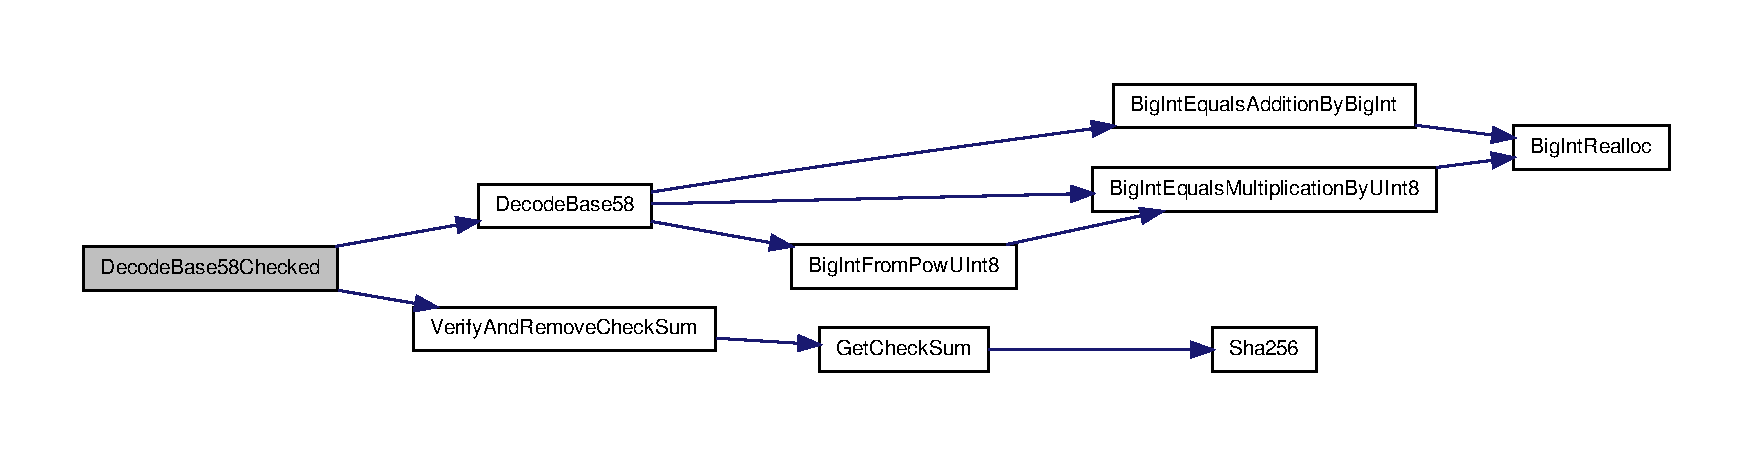
\includegraphics[width=400pt]{_base58_8c_a20b174879ad363a02444d6dfd0c3956f_cgraph}
\end{center}
\end{figure}


\hypertarget{_base58_8c_a8eba0d420462df41d21fa7369a9cf2de}{
\index{Base58.c@{Base58.c}!EncodeBase58@{EncodeBase58}}
\index{EncodeBase58@{EncodeBase58}!Base58.c@{Base58.c}}
\subsubsection[{EncodeBase58}]{\setlength{\rightskip}{0pt plus 5cm}char$\ast$ EncodeBase58 (
\begin{DoxyParamCaption}
\item[{uint8\_\-t $\ast$}]{bytes, }
\item[{uint8\_\-t}]{len}
\end{DoxyParamCaption}
)}}
\label{_base58_8c_a8eba0d420462df41d21fa7369a9cf2de}


Encodes byte data into base 58. 


\begin{DoxyParams}{Parameters}
{\em bytes} & Pointer to byte data to encode. Will almost certainly be modified. Copy data beforehand if needed. \\
\hline
{\em len} & Length of bytes to encode. \\
\hline
\end{DoxyParams}
\begin{DoxyReturn}{Returns}
Newly allocated string with encoded data or NULL on error. 
\end{DoxyReturn}


Definition at line 208 of file Base58.c.



Here is the call graph for this function:\nopagebreak
\begin{figure}[H]
\begin{center}
\leavevmode
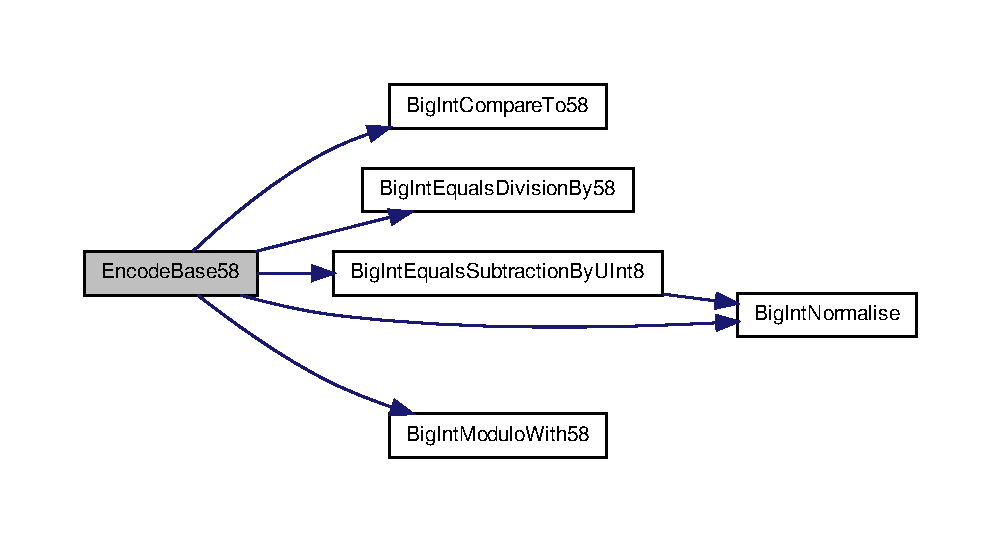
\includegraphics[width=400pt]{_base58_8c_a8eba0d420462df41d21fa7369a9cf2de_cgraph}
\end{center}
\end{figure}


\hypertarget{_base58_8c_a0e3eca914bcab6d9c960347ed24ca8d3}{
\index{Base58.c@{Base58.c}!GetCheckSum@{GetCheckSum}}
\index{GetCheckSum@{GetCheckSum}!Base58.c@{Base58.c}}
\subsubsection[{GetCheckSum}]{\setlength{\rightskip}{0pt plus 5cm}uint8\_\-t$\ast$ GetCheckSum (
\begin{DoxyParamCaption}
\item[{uint8\_\-t $\ast$}]{data}
\end{DoxyParamCaption}
)}}
\label{_base58_8c_a0e3eca914bcab6d9c960347ed24ca8d3}


Definition at line 282 of file Base58.c.



Here is the call graph for this function:\nopagebreak
\begin{figure}[H]
\begin{center}
\leavevmode
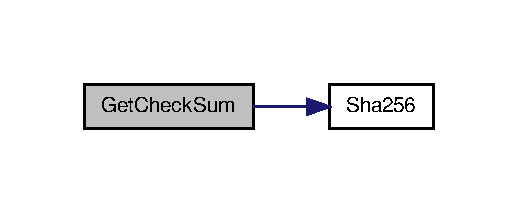
\includegraphics[width=248pt]{_base58_8c_a0e3eca914bcab6d9c960347ed24ca8d3_cgraph}
\end{center}
\end{figure}




Here is the caller graph for this function:\nopagebreak
\begin{figure}[H]
\begin{center}
\leavevmode
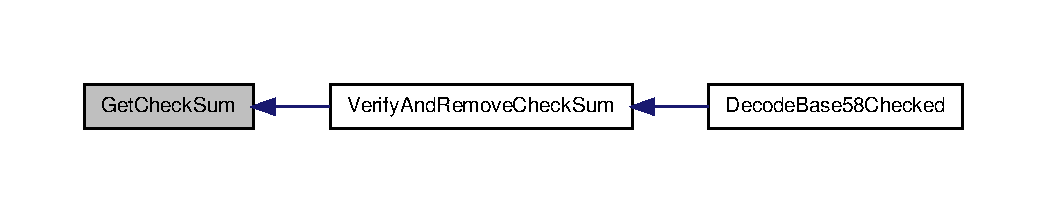
\includegraphics[width=400pt]{_base58_8c_a0e3eca914bcab6d9c960347ed24ca8d3_icgraph}
\end{center}
\end{figure}


\hypertarget{_base58_8c_a638fbbbf6ac769d7ac1e730437fce0c0}{
\index{Base58.c@{Base58.c}!VerifyAndRemoveCheckSum@{VerifyAndRemoveCheckSum}}
\index{VerifyAndRemoveCheckSum@{VerifyAndRemoveCheckSum}!Base58.c@{Base58.c}}
\subsubsection[{VerifyAndRemoveCheckSum}]{\setlength{\rightskip}{0pt plus 5cm}uint8\_\-t$\ast$ VerifyAndRemoveCheckSum (
\begin{DoxyParamCaption}
\item[{uint8\_\-t $\ast$}]{data}
\end{DoxyParamCaption}
)}}
\label{_base58_8c_a638fbbbf6ac769d7ac1e730437fce0c0}


Definition at line 113 of file Base58.c.



Here is the call graph for this function:\nopagebreak
\begin{figure}[H]
\begin{center}
\leavevmode
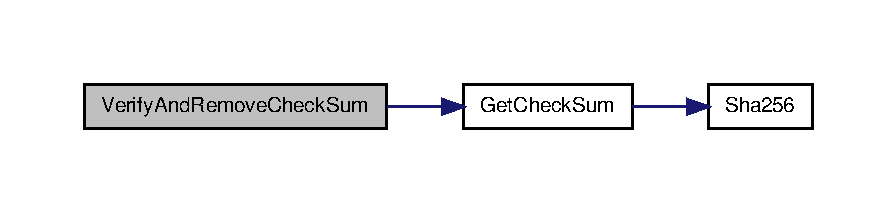
\includegraphics[width=400pt]{_base58_8c_a638fbbbf6ac769d7ac1e730437fce0c0_cgraph}
\end{center}
\end{figure}




Here is the caller graph for this function:\nopagebreak
\begin{figure}[H]
\begin{center}
\leavevmode
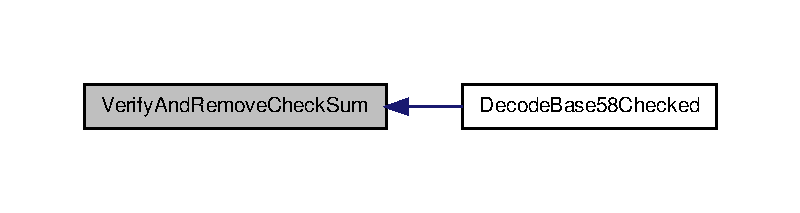
\includegraphics[width=384pt]{_base58_8c_a638fbbbf6ac769d7ac1e730437fce0c0_icgraph}
\end{center}
\end{figure}



\hypertarget{_base58_8h}{
\section{src/Base58/Base58.h File Reference}
\label{_base58_8h}\index{src/Base58/Base58.h@{src/Base58/Base58.h}}
}


Functions for encoding and decoding in base 58. Avoids 0olI whch may look alike. This is for readability concerns.  


{\ttfamily \#include $<$stdlib.h$>$}\par
{\ttfamily \#include \char`\"{}../BigInt/BigInt.h\char`\"{}}\par
Include dependency graph for Base58.h:\nopagebreak
\begin{figure}[H]
\begin{center}
\leavevmode
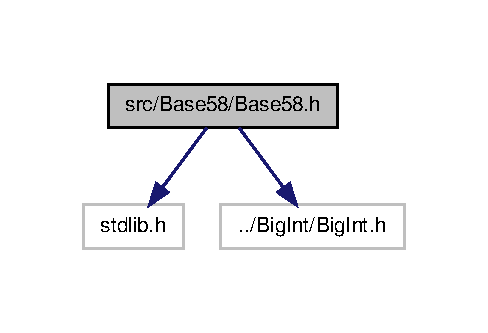
\includegraphics[width=234pt]{_base58_8h__incl}
\end{center}
\end{figure}
This graph shows which files directly or indirectly include this file:\nopagebreak
\begin{figure}[H]
\begin{center}
\leavevmode
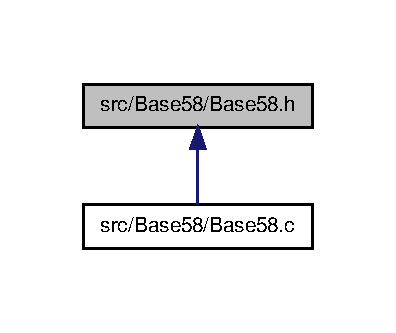
\includegraphics[width=190pt]{_base58_8h__dep__incl}
\end{center}
\end{figure}
\subsection*{Functions}
\begin{DoxyCompactItemize}
\item 
\hyperlink{struct_big_int}{BigInt} \hyperlink{_base58_8h_a698fb6717b2cbd17d02ff52b09d84fe5}{DecodeBase58} (char $\ast$str)
\begin{DoxyCompactList}\small\item\em Decodes base 58 string into byte data as a \hyperlink{struct_big_int}{BigInt}. \end{DoxyCompactList}\item 
\hyperlink{struct_big_int}{BigInt} \hyperlink{_base58_8h_a20b174879ad363a02444d6dfd0c3956f}{DecodeBase58Checked} (char $\ast$str, void($\ast$onErrorReceived)(\hyperlink{_constants_8h_a2c3e4bb40f36b262a5214e2da2bca9c5}{Error} error, char $\ast$,...))
\begin{DoxyCompactList}\small\item\em Decodes base 58 string into byte data as a \hyperlink{struct_big_int}{BigInt} and checks a 4 byte checksum. \end{DoxyCompactList}\item 
char $\ast$ \hyperlink{_base58_8h_a8eba0d420462df41d21fa7369a9cf2de}{EncodeBase58} (uint8\_\-t $\ast$bytes, uint8\_\-t len)
\begin{DoxyCompactList}\small\item\em Encodes byte data into base 58. \end{DoxyCompactList}\item 
uint8\_\-t $\ast$ \hyperlink{_base58_8h_a0e3eca914bcab6d9c960347ed24ca8d3}{GetCheckSum} (uint8\_\-t $\ast$data)
\item 
uint8\_\-t $\ast$ \hyperlink{_base58_8h_a638fbbbf6ac769d7ac1e730437fce0c0}{VerifyAndRemoveCheckSum} (uint8\_\-t $\ast$data)
\end{DoxyCompactItemize}


\subsection{Detailed Description}
Functions for encoding and decoding in base 58. Avoids 0olI whch may look alike. This is for readability concerns. 

Definition in file \hyperlink{_base58_8h_source}{Base58.h}.



\subsection{Function Documentation}
\hypertarget{_base58_8h_a698fb6717b2cbd17d02ff52b09d84fe5}{
\index{Base58.h@{Base58.h}!DecodeBase58@{DecodeBase58}}
\index{DecodeBase58@{DecodeBase58}!Base58.h@{Base58.h}}
\subsubsection[{DecodeBase58}]{\setlength{\rightskip}{0pt plus 5cm}{\bf BigInt} DecodeBase58 (
\begin{DoxyParamCaption}
\item[{char $\ast$}]{str}
\end{DoxyParamCaption}
)}}
\label{_base58_8h_a698fb6717b2cbd17d02ff52b09d84fe5}


Decodes base 58 string into byte data as a \hyperlink{struct_big_int}{BigInt}. 


\begin{DoxyParams}{Parameters}
{\em str} & Base 58 string to decode. \\
\hline
\end{DoxyParams}
\begin{DoxyReturn}{Returns}
Pointer to the byte data as a \hyperlink{struct_big_int}{BigInt}. The byte data will be created in this function. Remember to free the data. On error the big int will have a NULL data pointer. 
\end{DoxyReturn}


Definition at line 14 of file Base58.c.



Here is the call graph for this function:\nopagebreak
\begin{figure}[H]
\begin{center}
\leavevmode
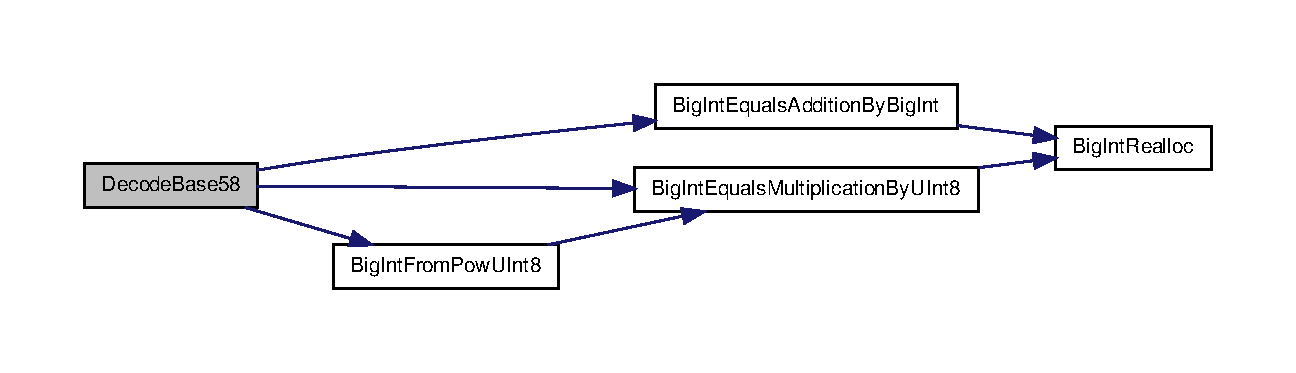
\includegraphics[width=400pt]{_base58_8h_a698fb6717b2cbd17d02ff52b09d84fe5_cgraph}
\end{center}
\end{figure}




Here is the caller graph for this function:\nopagebreak
\begin{figure}[H]
\begin{center}
\leavevmode
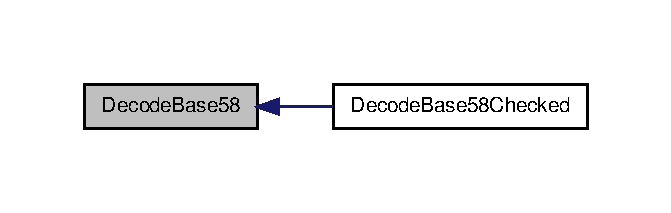
\includegraphics[width=322pt]{_base58_8h_a698fb6717b2cbd17d02ff52b09d84fe5_icgraph}
\end{center}
\end{figure}


\hypertarget{_base58_8h_a20b174879ad363a02444d6dfd0c3956f}{
\index{Base58.h@{Base58.h}!DecodeBase58Checked@{DecodeBase58Checked}}
\index{DecodeBase58Checked@{DecodeBase58Checked}!Base58.h@{Base58.h}}
\subsubsection[{DecodeBase58Checked}]{\setlength{\rightskip}{0pt plus 5cm}{\bf BigInt} DecodeBase58Checked (
\begin{DoxyParamCaption}
\item[{char $\ast$}]{str, }
\item[{void($\ast$)({\bf Error} error, char $\ast$,...)}]{onErrorReceived}
\end{DoxyParamCaption}
)}}
\label{_base58_8h_a20b174879ad363a02444d6dfd0c3956f}


Decodes base 58 string into byte data as a \hyperlink{struct_big_int}{BigInt} and checks a 4 byte checksum. 


\begin{DoxyParams}{Parameters}
{\em str} & Base 58 string to decode. \\
\hline
\end{DoxyParams}
\begin{DoxyReturn}{Returns}
Byte data as a \hyperlink{struct_big_int}{BigInt}. Is zero on failure. Checksum is included in returned data. On error the big int will have a NULL data pointer. 
\end{DoxyReturn}


Definition at line 128 of file Base58.c.



Here is the call graph for this function:\nopagebreak
\begin{figure}[H]
\begin{center}
\leavevmode
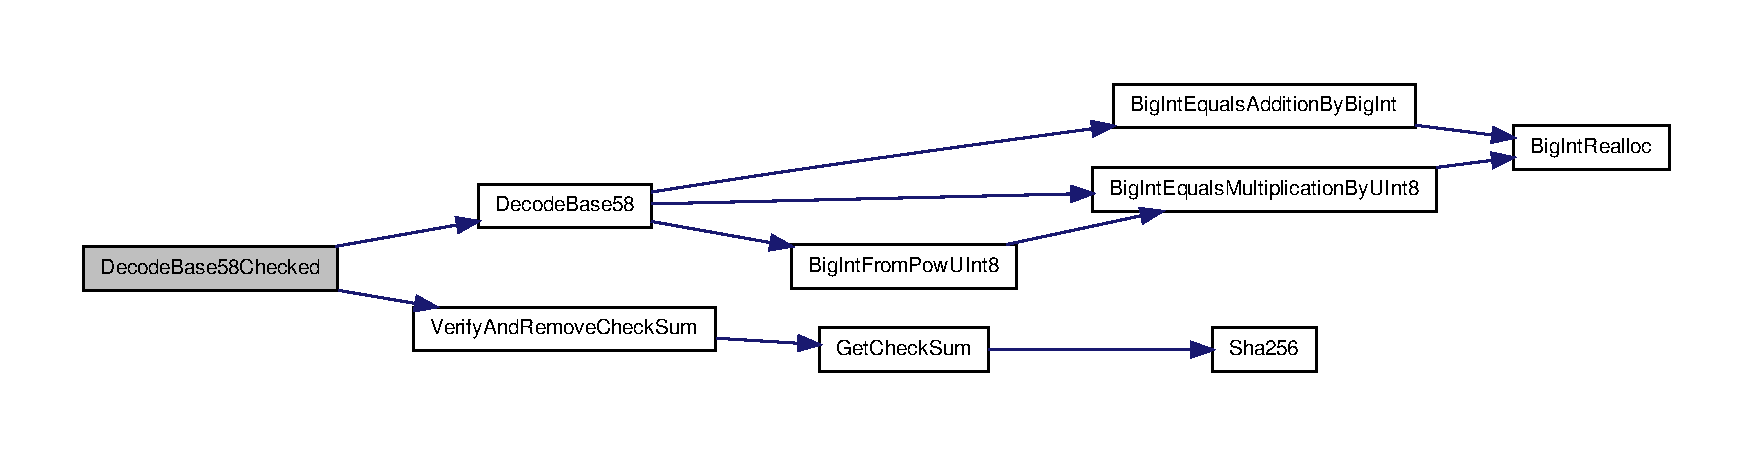
\includegraphics[width=400pt]{_base58_8h_a20b174879ad363a02444d6dfd0c3956f_cgraph}
\end{center}
\end{figure}


\hypertarget{_base58_8h_a8eba0d420462df41d21fa7369a9cf2de}{
\index{Base58.h@{Base58.h}!EncodeBase58@{EncodeBase58}}
\index{EncodeBase58@{EncodeBase58}!Base58.h@{Base58.h}}
\subsubsection[{EncodeBase58}]{\setlength{\rightskip}{0pt plus 5cm}char$\ast$ EncodeBase58 (
\begin{DoxyParamCaption}
\item[{uint8\_\-t $\ast$}]{bytes, }
\item[{uint8\_\-t}]{len}
\end{DoxyParamCaption}
)}}
\label{_base58_8h_a8eba0d420462df41d21fa7369a9cf2de}


Encodes byte data into base 58. 


\begin{DoxyParams}{Parameters}
{\em bytes} & Pointer to byte data to encode. Will almost certainly be modified. Copy data beforehand if needed. \\
\hline
{\em len} & Length of bytes to encode. \\
\hline
\end{DoxyParams}
\begin{DoxyReturn}{Returns}
Newly allocated string with encoded data or NULL on error. 
\end{DoxyReturn}


Definition at line 208 of file Base58.c.



Here is the call graph for this function:\nopagebreak
\begin{figure}[H]
\begin{center}
\leavevmode
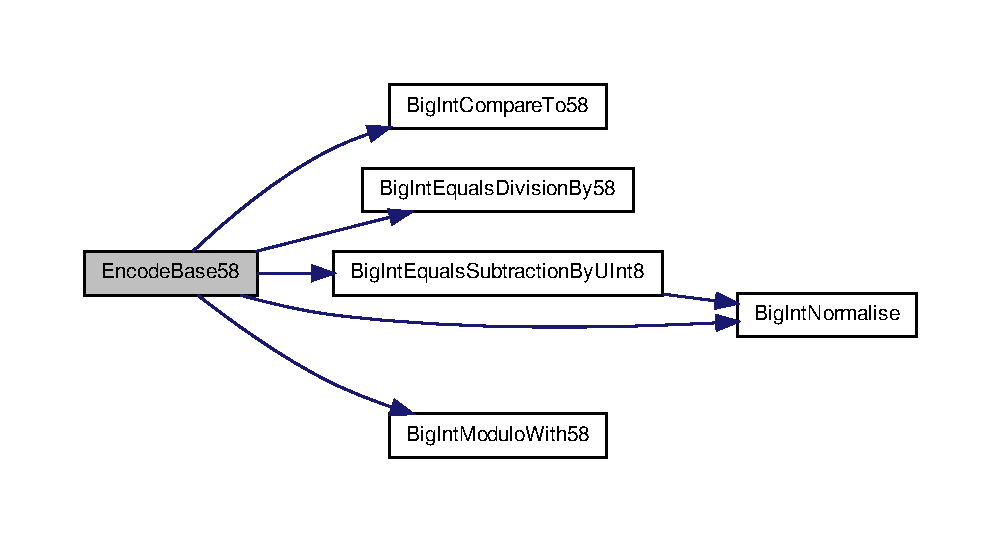
\includegraphics[width=400pt]{_base58_8h_a8eba0d420462df41d21fa7369a9cf2de_cgraph}
\end{center}
\end{figure}


\hypertarget{_base58_8h_a0e3eca914bcab6d9c960347ed24ca8d3}{
\index{Base58.h@{Base58.h}!GetCheckSum@{GetCheckSum}}
\index{GetCheckSum@{GetCheckSum}!Base58.h@{Base58.h}}
\subsubsection[{GetCheckSum}]{\setlength{\rightskip}{0pt plus 5cm}uint8\_\-t$\ast$ GetCheckSum (
\begin{DoxyParamCaption}
\item[{uint8\_\-t $\ast$}]{data}
\end{DoxyParamCaption}
)}}
\label{_base58_8h_a0e3eca914bcab6d9c960347ed24ca8d3}


Definition at line 282 of file Base58.c.



Here is the call graph for this function:\nopagebreak
\begin{figure}[H]
\begin{center}
\leavevmode
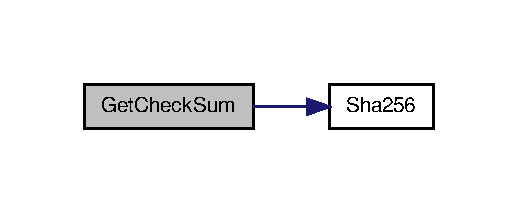
\includegraphics[width=248pt]{_base58_8h_a0e3eca914bcab6d9c960347ed24ca8d3_cgraph}
\end{center}
\end{figure}




Here is the caller graph for this function:\nopagebreak
\begin{figure}[H]
\begin{center}
\leavevmode
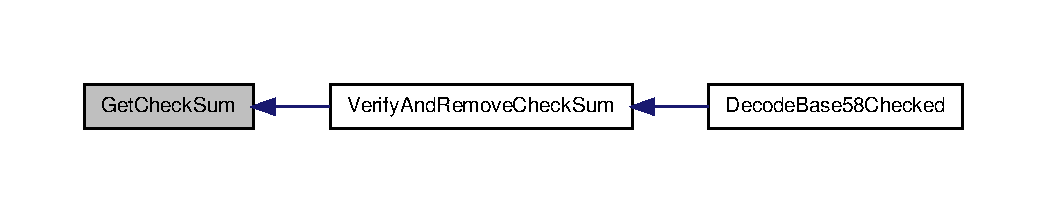
\includegraphics[width=400pt]{_base58_8h_a0e3eca914bcab6d9c960347ed24ca8d3_icgraph}
\end{center}
\end{figure}


\hypertarget{_base58_8h_a638fbbbf6ac769d7ac1e730437fce0c0}{
\index{Base58.h@{Base58.h}!VerifyAndRemoveCheckSum@{VerifyAndRemoveCheckSum}}
\index{VerifyAndRemoveCheckSum@{VerifyAndRemoveCheckSum}!Base58.h@{Base58.h}}
\subsubsection[{VerifyAndRemoveCheckSum}]{\setlength{\rightskip}{0pt plus 5cm}uint8\_\-t$\ast$ VerifyAndRemoveCheckSum (
\begin{DoxyParamCaption}
\item[{uint8\_\-t $\ast$}]{data}
\end{DoxyParamCaption}
)}}
\label{_base58_8h_a638fbbbf6ac769d7ac1e730437fce0c0}


Definition at line 113 of file Base58.c.



Here is the call graph for this function:\nopagebreak
\begin{figure}[H]
\begin{center}
\leavevmode
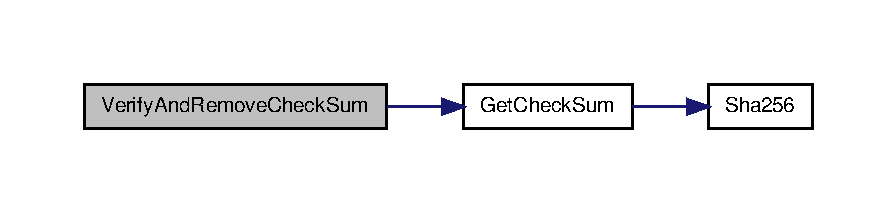
\includegraphics[width=400pt]{_base58_8h_a638fbbbf6ac769d7ac1e730437fce0c0_cgraph}
\end{center}
\end{figure}




Here is the caller graph for this function:\nopagebreak
\begin{figure}[H]
\begin{center}
\leavevmode
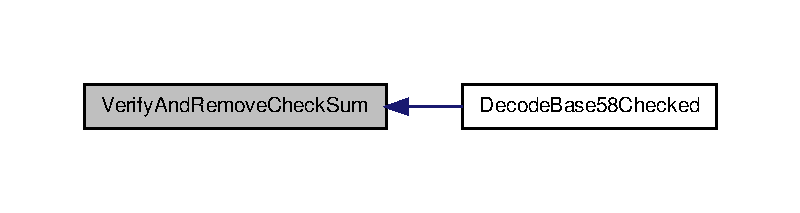
\includegraphics[width=384pt]{_base58_8h_a638fbbbf6ac769d7ac1e730437fce0c0_icgraph}
\end{center}
\end{figure}



\hypertarget{_big_int_8c}{
\section{src/BigInt/BigInt.c File Reference}
\label{_big_int_8c}\index{src/BigInt/BigInt.c@{src/BigInt/BigInt.c}}
}
{\ttfamily \#include \char`\"{}BigInt.h\char`\"{}}\par
{\ttfamily \#include $<$assert.h$>$}\par
{\ttfamily \#include $<$stdbool.h$>$}\par
Include dependency graph for BigInt.c:\nopagebreak
\begin{figure}[H]
\begin{center}
\leavevmode
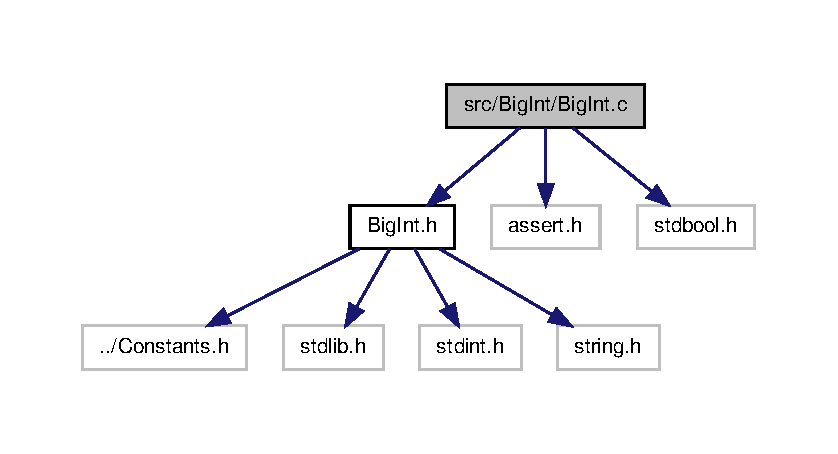
\includegraphics[width=400pt]{_big_int_8c__incl}
\end{center}
\end{figure}
\subsection*{Functions}
\begin{DoxyCompactItemize}
\item 
int \hyperlink{_big_int_8c_a5742814e569802287b7157f5ee150daa}{BigIntAlloc} (\hyperlink{struct_big_int}{BigInt} $\ast$bi, uint8\_\-t length)
\item 
int \hyperlink{_big_int_8c_acb40846a8d9132c888e78cd773382561}{BigIntRealloc} (\hyperlink{struct_big_int}{BigInt} $\ast$bi, uint8\_\-t length)
\item 
\hyperlink{_constants_8h_af5e6c1e42f1dbe27251f73c8b89d2504}{Compare} \hyperlink{_big_int_8c_a766564219de39ebab49e86b84365155d}{BigIntCompareTo58} (\hyperlink{struct_big_int}{BigInt} $\ast$a)
\item 
int \hyperlink{_big_int_8c_aceb9c4c6e4716127e4fc6d964b135527}{BigIntEqualsAdditionByBigInt} (\hyperlink{struct_big_int}{BigInt} $\ast$a, \hyperlink{struct_big_int}{BigInt} $\ast$b)
\item 
void \hyperlink{_big_int_8c_ac1d1b61df392b26380337c98e859a295}{BigIntEqualsDivisionBy58} (\hyperlink{struct_big_int}{BigInt} $\ast$a, uint8\_\-t $\ast$ans)
\item 
int \hyperlink{_big_int_8c_abadebe4d6bc13cecd5434dcd4607c0e8}{BigIntEqualsMultiplicationByUInt8} (\hyperlink{struct_big_int}{BigInt} $\ast$a, uint8\_\-t b, uint8\_\-t $\ast$ans)
\item 
void \hyperlink{_big_int_8c_a9d2029aadab4a8ae5f376d3059786394}{BigIntEqualsSubtractionByUInt8} (\hyperlink{struct_big_int}{BigInt} $\ast$a, uint8\_\-t b)
\item 
int \hyperlink{_big_int_8c_a7544af9d148635904d1809eef62c11ae}{BigIntFromPowUInt8} (\hyperlink{struct_big_int}{BigInt} $\ast$bi, uint8\_\-t a, uint8\_\-t b)
\item 
uint8\_\-t \hyperlink{_big_int_8c_aa4544c75bd8e7106208d9b120d2bb533}{BigIntModuloWith58} (\hyperlink{struct_big_int}{BigInt} $\ast$a)
\item 
void \hyperlink{_big_int_8c_a980d453cb2c16efd376b928800c189ab}{BigIntNormalise} (\hyperlink{struct_big_int}{BigInt} $\ast$a)
\end{DoxyCompactItemize}


\subsection{Function Documentation}
\hypertarget{_big_int_8c_a5742814e569802287b7157f5ee150daa}{
\index{BigInt.c@{BigInt.c}!BigIntAlloc@{BigIntAlloc}}
\index{BigIntAlloc@{BigIntAlloc}!BigInt.c@{BigInt.c}}
\subsubsection[{BigIntAlloc}]{\setlength{\rightskip}{0pt plus 5cm}int BigIntAlloc (
\begin{DoxyParamCaption}
\item[{{\bf BigInt} $\ast$}]{bi, }
\item[{uint8\_\-t}]{length}
\end{DoxyParamCaption}
)}}
\label{_big_int_8c_a5742814e569802287b7157f5ee150daa}


Definition at line 12 of file BigInt.c.



Here is the caller graph for this function:\nopagebreak
\begin{figure}[H]
\begin{center}
\leavevmode
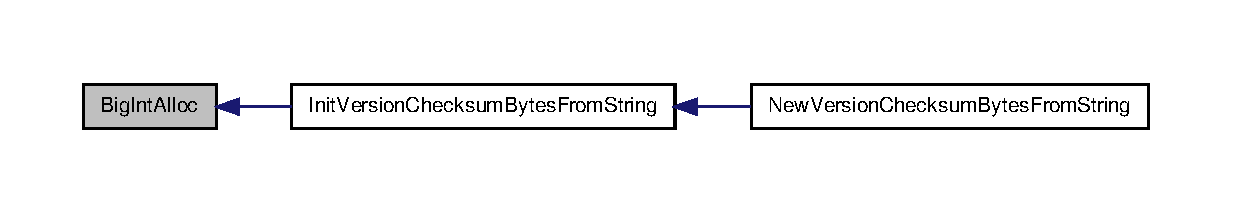
\includegraphics[width=400pt]{_big_int_8c_a5742814e569802287b7157f5ee150daa_icgraph}
\end{center}
\end{figure}


\hypertarget{_big_int_8c_a766564219de39ebab49e86b84365155d}{
\index{BigInt.c@{BigInt.c}!BigIntCompareTo58@{BigIntCompareTo58}}
\index{BigIntCompareTo58@{BigIntCompareTo58}!BigInt.c@{BigInt.c}}
\subsubsection[{BigIntCompareTo58}]{\setlength{\rightskip}{0pt plus 5cm}{\bf Compare} BigIntCompareTo58 (
\begin{DoxyParamCaption}
\item[{{\bf BigInt} $\ast$}]{a}
\end{DoxyParamCaption}
)}}
\label{_big_int_8c_a766564219de39ebab49e86b84365155d}


Definition at line 29 of file BigInt.c.



Here is the caller graph for this function:\nopagebreak
\begin{figure}[H]
\begin{center}
\leavevmode
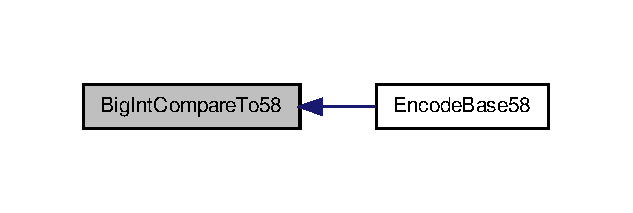
\includegraphics[width=304pt]{_big_int_8c_a766564219de39ebab49e86b84365155d_icgraph}
\end{center}
\end{figure}


\hypertarget{_big_int_8c_aceb9c4c6e4716127e4fc6d964b135527}{
\index{BigInt.c@{BigInt.c}!BigIntEqualsAdditionByBigInt@{BigIntEqualsAdditionByBigInt}}
\index{BigIntEqualsAdditionByBigInt@{BigIntEqualsAdditionByBigInt}!BigInt.c@{BigInt.c}}
\subsubsection[{BigIntEqualsAdditionByBigInt}]{\setlength{\rightskip}{0pt plus 5cm}int BigIntEqualsAdditionByBigInt (
\begin{DoxyParamCaption}
\item[{{\bf BigInt} $\ast$}]{a, }
\item[{{\bf BigInt} $\ast$}]{b}
\end{DoxyParamCaption}
)}}
\label{_big_int_8c_aceb9c4c6e4716127e4fc6d964b135527}


Definition at line 55 of file BigInt.c.



Here is the call graph for this function:\nopagebreak
\begin{figure}[H]
\begin{center}
\leavevmode
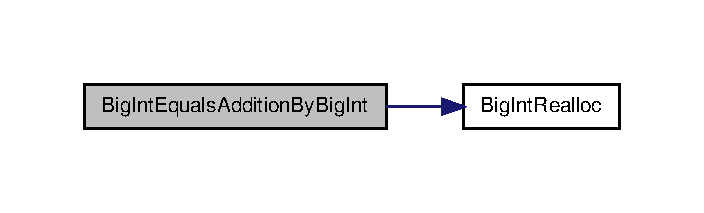
\includegraphics[width=338pt]{_big_int_8c_aceb9c4c6e4716127e4fc6d964b135527_cgraph}
\end{center}
\end{figure}




Here is the caller graph for this function:\nopagebreak
\begin{figure}[H]
\begin{center}
\leavevmode
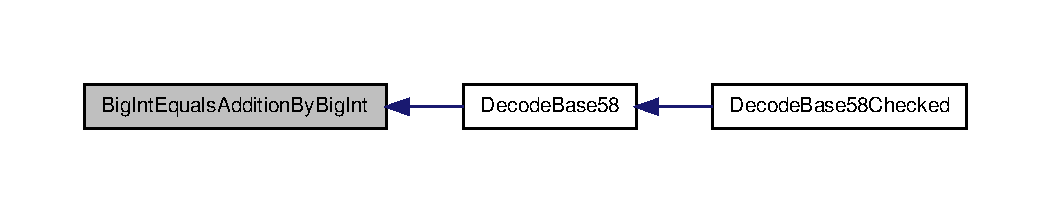
\includegraphics[width=400pt]{_big_int_8c_aceb9c4c6e4716127e4fc6d964b135527_icgraph}
\end{center}
\end{figure}


\hypertarget{_big_int_8c_ac1d1b61df392b26380337c98e859a295}{
\index{BigInt.c@{BigInt.c}!BigIntEqualsDivisionBy58@{BigIntEqualsDivisionBy58}}
\index{BigIntEqualsDivisionBy58@{BigIntEqualsDivisionBy58}!BigInt.c@{BigInt.c}}
\subsubsection[{BigIntEqualsDivisionBy58}]{\setlength{\rightskip}{0pt plus 5cm}void BigIntEqualsDivisionBy58 (
\begin{DoxyParamCaption}
\item[{{\bf BigInt} $\ast$}]{a, }
\item[{uint8\_\-t $\ast$}]{ans}
\end{DoxyParamCaption}
)}}
\label{_big_int_8c_ac1d1b61df392b26380337c98e859a295}


Definition at line 84 of file BigInt.c.



Here is the caller graph for this function:\nopagebreak
\begin{figure}[H]
\begin{center}
\leavevmode
\includegraphics[width=330pt]{_big_int_8c_ac1d1b61df392b26380337c98e859a295_icgraph}
\end{center}
\end{figure}


\hypertarget{_big_int_8c_abadebe4d6bc13cecd5434dcd4607c0e8}{
\index{BigInt.c@{BigInt.c}!BigIntEqualsMultiplicationByUInt8@{BigIntEqualsMultiplicationByUInt8}}
\index{BigIntEqualsMultiplicationByUInt8@{BigIntEqualsMultiplicationByUInt8}!BigInt.c@{BigInt.c}}
\subsubsection[{BigIntEqualsMultiplicationByUInt8}]{\setlength{\rightskip}{0pt plus 5cm}int BigIntEqualsMultiplicationByUInt8 (
\begin{DoxyParamCaption}
\item[{{\bf BigInt} $\ast$}]{a, }
\item[{uint8\_\-t}]{b, }
\item[{uint8\_\-t $\ast$}]{ans}
\end{DoxyParamCaption}
)}}
\label{_big_int_8c_abadebe4d6bc13cecd5434dcd4607c0e8}


Definition at line 102 of file BigInt.c.



Here is the call graph for this function:\nopagebreak
\begin{figure}[H]
\begin{center}
\leavevmode
\includegraphics[width=358pt]{_big_int_8c_abadebe4d6bc13cecd5434dcd4607c0e8_cgraph}
\end{center}
\end{figure}




Here is the caller graph for this function:\nopagebreak
\begin{figure}[H]
\begin{center}
\leavevmode
\includegraphics[width=400pt]{_big_int_8c_abadebe4d6bc13cecd5434dcd4607c0e8_icgraph}
\end{center}
\end{figure}


\hypertarget{_big_int_8c_a9d2029aadab4a8ae5f376d3059786394}{
\index{BigInt.c@{BigInt.c}!BigIntEqualsSubtractionByUInt8@{BigIntEqualsSubtractionByUInt8}}
\index{BigIntEqualsSubtractionByUInt8@{BigIntEqualsSubtractionByUInt8}!BigInt.c@{BigInt.c}}
\subsubsection[{BigIntEqualsSubtractionByUInt8}]{\setlength{\rightskip}{0pt plus 5cm}void BigIntEqualsSubtractionByUInt8 (
\begin{DoxyParamCaption}
\item[{{\bf BigInt} $\ast$}]{a, }
\item[{uint8\_\-t}]{b}
\end{DoxyParamCaption}
)}}
\label{_big_int_8c_a9d2029aadab4a8ae5f376d3059786394}


Definition at line 144 of file BigInt.c.



Here is the call graph for this function:\nopagebreak
\begin{figure}[H]
\begin{center}
\leavevmode
\includegraphics[width=360pt]{_big_int_8c_a9d2029aadab4a8ae5f376d3059786394_cgraph}
\end{center}
\end{figure}




Here is the caller graph for this function:\nopagebreak
\begin{figure}[H]
\begin{center}
\leavevmode
\includegraphics[width=358pt]{_big_int_8c_a9d2029aadab4a8ae5f376d3059786394_icgraph}
\end{center}
\end{figure}


\hypertarget{_big_int_8c_a7544af9d148635904d1809eef62c11ae}{
\index{BigInt.c@{BigInt.c}!BigIntFromPowUInt8@{BigIntFromPowUInt8}}
\index{BigIntFromPowUInt8@{BigIntFromPowUInt8}!BigInt.c@{BigInt.c}}
\subsubsection[{BigIntFromPowUInt8}]{\setlength{\rightskip}{0pt plus 5cm}int BigIntFromPowUInt8 (
\begin{DoxyParamCaption}
\item[{{\bf BigInt} $\ast$}]{bi, }
\item[{uint8\_\-t}]{a, }
\item[{uint8\_\-t}]{b}
\end{DoxyParamCaption}
)}}
\label{_big_int_8c_a7544af9d148635904d1809eef62c11ae}


Definition at line 160 of file BigInt.c.



Here is the call graph for this function:\nopagebreak
\begin{figure}[H]
\begin{center}
\leavevmode
\includegraphics[width=400pt]{_big_int_8c_a7544af9d148635904d1809eef62c11ae_cgraph}
\end{center}
\end{figure}




Here is the caller graph for this function:\nopagebreak
\begin{figure}[H]
\begin{center}
\leavevmode
\includegraphics[width=400pt]{_big_int_8c_a7544af9d148635904d1809eef62c11ae_icgraph}
\end{center}
\end{figure}


\hypertarget{_big_int_8c_aa4544c75bd8e7106208d9b120d2bb533}{
\index{BigInt.c@{BigInt.c}!BigIntModuloWith58@{BigIntModuloWith58}}
\index{BigIntModuloWith58@{BigIntModuloWith58}!BigInt.c@{BigInt.c}}
\subsubsection[{BigIntModuloWith58}]{\setlength{\rightskip}{0pt plus 5cm}uint8\_\-t BigIntModuloWith58 (
\begin{DoxyParamCaption}
\item[{{\bf BigInt} $\ast$}]{a}
\end{DoxyParamCaption}
)}}
\label{_big_int_8c_aa4544c75bd8e7106208d9b120d2bb533}


Definition at line 180 of file BigInt.c.



Here is the caller graph for this function:\nopagebreak
\begin{figure}[H]
\begin{center}
\leavevmode
\includegraphics[width=304pt]{_big_int_8c_aa4544c75bd8e7106208d9b120d2bb533_icgraph}
\end{center}
\end{figure}


\hypertarget{_big_int_8c_a980d453cb2c16efd376b928800c189ab}{
\index{BigInt.c@{BigInt.c}!BigIntNormalise@{BigIntNormalise}}
\index{BigIntNormalise@{BigIntNormalise}!BigInt.c@{BigInt.c}}
\subsubsection[{BigIntNormalise}]{\setlength{\rightskip}{0pt plus 5cm}void BigIntNormalise (
\begin{DoxyParamCaption}
\item[{{\bf BigInt} $\ast$}]{a}
\end{DoxyParamCaption}
)}}
\label{_big_int_8c_a980d453cb2c16efd376b928800c189ab}


Definition at line 193 of file BigInt.c.



Here is the caller graph for this function:\nopagebreak
\begin{figure}[H]
\begin{center}
\leavevmode
\includegraphics[width=400pt]{_big_int_8c_a980d453cb2c16efd376b928800c189ab_icgraph}
\end{center}
\end{figure}


\hypertarget{_big_int_8c_acb40846a8d9132c888e78cd773382561}{
\index{BigInt.c@{BigInt.c}!BigIntRealloc@{BigIntRealloc}}
\index{BigIntRealloc@{BigIntRealloc}!BigInt.c@{BigInt.c}}
\subsubsection[{BigIntRealloc}]{\setlength{\rightskip}{0pt plus 5cm}int BigIntRealloc (
\begin{DoxyParamCaption}
\item[{{\bf BigInt} $\ast$}]{bi, }
\item[{uint8\_\-t}]{length}
\end{DoxyParamCaption}
)}}
\label{_big_int_8c_acb40846a8d9132c888e78cd773382561}


Definition at line 18 of file BigInt.c.



Here is the caller graph for this function:\nopagebreak
\begin{figure}[H]
\begin{center}
\leavevmode
\includegraphics[width=400pt]{_big_int_8c_acb40846a8d9132c888e78cd773382561_icgraph}
\end{center}
\end{figure}



\hypertarget{_big_int_8h}{
\section{src/BigInt/BigInt.h File Reference}
\label{_big_int_8h}\index{src/BigInt/BigInt.h@{src/BigInt/BigInt.h}}
}
{\ttfamily \#include \char`\"{}../Constants.h\char`\"{}}\par
{\ttfamily \#include $<$stdlib.h$>$}\par
{\ttfamily \#include $<$stdint.h$>$}\par
{\ttfamily \#include $<$string.h$>$}\par
Include dependency graph for BigInt.h:\nopagebreak
\begin{figure}[H]
\begin{center}
\leavevmode
\includegraphics[width=356pt]{_big_int_8h__incl}
\end{center}
\end{figure}
This graph shows which files directly or indirectly include this file:\nopagebreak
\begin{figure}[H]
\begin{center}
\leavevmode
\includegraphics[width=302pt]{_big_int_8h__dep__incl}
\end{center}
\end{figure}
\subsection*{Data Structures}
\begin{DoxyCompactItemize}
\item 
struct \hyperlink{struct_big_int}{BigInt}
\begin{DoxyCompactList}\small\item\em Contains byte data with the length of this data to represent a large integer. The byte data is in little-\/endian which stores the smallest byte first. On an error data is set to NULL and length is 0. \end{DoxyCompactList}\end{DoxyCompactItemize}
\subsection*{Functions}
\begin{DoxyCompactItemize}
\item 
int \hyperlink{_big_int_8h_a7544af9d148635904d1809eef62c11ae}{BigIntFromPowUInt8} (\hyperlink{struct_big_int}{BigInt} $\ast$bi, uint8\_\-t a, uint8\_\-t b)
\item 
int \hyperlink{_big_int_8h_abadebe4d6bc13cecd5434dcd4607c0e8}{BigIntEqualsMultiplicationByUInt8} (\hyperlink{struct_big_int}{BigInt} $\ast$a, uint8\_\-t b, uint8\_\-t $\ast$ans)
\item 
int \hyperlink{_big_int_8h_aceb9c4c6e4716127e4fc6d964b135527}{BigIntEqualsAdditionByBigInt} (\hyperlink{struct_big_int}{BigInt} $\ast$a, \hyperlink{struct_big_int}{BigInt} $\ast$b)
\item 
void \hyperlink{_big_int_8h_a980d453cb2c16efd376b928800c189ab}{BigIntNormalise} (\hyperlink{struct_big_int}{BigInt} $\ast$a)
\item 
uint8\_\-t \hyperlink{_big_int_8h_aa4544c75bd8e7106208d9b120d2bb533}{BigIntModuloWith58} (\hyperlink{struct_big_int}{BigInt} $\ast$a)
\item 
void \hyperlink{_big_int_8h_a9d2029aadab4a8ae5f376d3059786394}{BigIntEqualsSubtractionByUInt8} (\hyperlink{struct_big_int}{BigInt} $\ast$a, uint8\_\-t b)
\item 
void \hyperlink{_big_int_8h_ac1d1b61df392b26380337c98e859a295}{BigIntEqualsDivisionBy58} (\hyperlink{struct_big_int}{BigInt} $\ast$a, uint8\_\-t $\ast$ans)
\item 
\hyperlink{_constants_8h_af5e6c1e42f1dbe27251f73c8b89d2504}{Compare} \hyperlink{_big_int_8h_a766564219de39ebab49e86b84365155d}{BigIntCompareTo58} (\hyperlink{struct_big_int}{BigInt} $\ast$a)
\end{DoxyCompactItemize}


\subsection{Function Documentation}
\hypertarget{_big_int_8h_a766564219de39ebab49e86b84365155d}{
\index{BigInt.h@{BigInt.h}!BigIntCompareTo58@{BigIntCompareTo58}}
\index{BigIntCompareTo58@{BigIntCompareTo58}!BigInt.h@{BigInt.h}}
\subsubsection[{BigIntCompareTo58}]{\setlength{\rightskip}{0pt plus 5cm}{\bf Compare} BigIntCompareTo58 (
\begin{DoxyParamCaption}
\item[{{\bf BigInt} $\ast$}]{a}
\end{DoxyParamCaption}
)}}
\label{_big_int_8h_a766564219de39ebab49e86b84365155d}


Definition at line 29 of file BigInt.c.



Here is the caller graph for this function:\nopagebreak
\begin{figure}[H]
\begin{center}
\leavevmode
\includegraphics[width=304pt]{_big_int_8h_a766564219de39ebab49e86b84365155d_icgraph}
\end{center}
\end{figure}


\hypertarget{_big_int_8h_aceb9c4c6e4716127e4fc6d964b135527}{
\index{BigInt.h@{BigInt.h}!BigIntEqualsAdditionByBigInt@{BigIntEqualsAdditionByBigInt}}
\index{BigIntEqualsAdditionByBigInt@{BigIntEqualsAdditionByBigInt}!BigInt.h@{BigInt.h}}
\subsubsection[{BigIntEqualsAdditionByBigInt}]{\setlength{\rightskip}{0pt plus 5cm}int BigIntEqualsAdditionByBigInt (
\begin{DoxyParamCaption}
\item[{{\bf BigInt} $\ast$}]{a, }
\item[{{\bf BigInt} $\ast$}]{b}
\end{DoxyParamCaption}
)}}
\label{_big_int_8h_aceb9c4c6e4716127e4fc6d964b135527}


Definition at line 55 of file BigInt.c.



Here is the call graph for this function:\nopagebreak
\begin{figure}[H]
\begin{center}
\leavevmode
\includegraphics[width=338pt]{_big_int_8h_aceb9c4c6e4716127e4fc6d964b135527_cgraph}
\end{center}
\end{figure}




Here is the caller graph for this function:\nopagebreak
\begin{figure}[H]
\begin{center}
\leavevmode
\includegraphics[width=400pt]{_big_int_8h_aceb9c4c6e4716127e4fc6d964b135527_icgraph}
\end{center}
\end{figure}


\hypertarget{_big_int_8h_ac1d1b61df392b26380337c98e859a295}{
\index{BigInt.h@{BigInt.h}!BigIntEqualsDivisionBy58@{BigIntEqualsDivisionBy58}}
\index{BigIntEqualsDivisionBy58@{BigIntEqualsDivisionBy58}!BigInt.h@{BigInt.h}}
\subsubsection[{BigIntEqualsDivisionBy58}]{\setlength{\rightskip}{0pt plus 5cm}void BigIntEqualsDivisionBy58 (
\begin{DoxyParamCaption}
\item[{{\bf BigInt} $\ast$}]{a, }
\item[{uint8\_\-t $\ast$}]{ans}
\end{DoxyParamCaption}
)}}
\label{_big_int_8h_ac1d1b61df392b26380337c98e859a295}


Definition at line 84 of file BigInt.c.



Here is the caller graph for this function:\nopagebreak
\begin{figure}[H]
\begin{center}
\leavevmode
\includegraphics[width=330pt]{_big_int_8h_ac1d1b61df392b26380337c98e859a295_icgraph}
\end{center}
\end{figure}


\hypertarget{_big_int_8h_abadebe4d6bc13cecd5434dcd4607c0e8}{
\index{BigInt.h@{BigInt.h}!BigIntEqualsMultiplicationByUInt8@{BigIntEqualsMultiplicationByUInt8}}
\index{BigIntEqualsMultiplicationByUInt8@{BigIntEqualsMultiplicationByUInt8}!BigInt.h@{BigInt.h}}
\subsubsection[{BigIntEqualsMultiplicationByUInt8}]{\setlength{\rightskip}{0pt plus 5cm}int BigIntEqualsMultiplicationByUInt8 (
\begin{DoxyParamCaption}
\item[{{\bf BigInt} $\ast$}]{a, }
\item[{uint8\_\-t}]{b, }
\item[{uint8\_\-t $\ast$}]{ans}
\end{DoxyParamCaption}
)}}
\label{_big_int_8h_abadebe4d6bc13cecd5434dcd4607c0e8}


Definition at line 102 of file BigInt.c.



Here is the call graph for this function:\nopagebreak
\begin{figure}[H]
\begin{center}
\leavevmode
\includegraphics[width=358pt]{_big_int_8h_abadebe4d6bc13cecd5434dcd4607c0e8_cgraph}
\end{center}
\end{figure}




Here is the caller graph for this function:\nopagebreak
\begin{figure}[H]
\begin{center}
\leavevmode
\includegraphics[width=400pt]{_big_int_8h_abadebe4d6bc13cecd5434dcd4607c0e8_icgraph}
\end{center}
\end{figure}


\hypertarget{_big_int_8h_a9d2029aadab4a8ae5f376d3059786394}{
\index{BigInt.h@{BigInt.h}!BigIntEqualsSubtractionByUInt8@{BigIntEqualsSubtractionByUInt8}}
\index{BigIntEqualsSubtractionByUInt8@{BigIntEqualsSubtractionByUInt8}!BigInt.h@{BigInt.h}}
\subsubsection[{BigIntEqualsSubtractionByUInt8}]{\setlength{\rightskip}{0pt plus 5cm}void BigIntEqualsSubtractionByUInt8 (
\begin{DoxyParamCaption}
\item[{{\bf BigInt} $\ast$}]{a, }
\item[{uint8\_\-t}]{b}
\end{DoxyParamCaption}
)}}
\label{_big_int_8h_a9d2029aadab4a8ae5f376d3059786394}


Definition at line 144 of file BigInt.c.



Here is the call graph for this function:\nopagebreak
\begin{figure}[H]
\begin{center}
\leavevmode
\includegraphics[width=360pt]{_big_int_8h_a9d2029aadab4a8ae5f376d3059786394_cgraph}
\end{center}
\end{figure}




Here is the caller graph for this function:\nopagebreak
\begin{figure}[H]
\begin{center}
\leavevmode
\includegraphics[width=358pt]{_big_int_8h_a9d2029aadab4a8ae5f376d3059786394_icgraph}
\end{center}
\end{figure}


\hypertarget{_big_int_8h_a7544af9d148635904d1809eef62c11ae}{
\index{BigInt.h@{BigInt.h}!BigIntFromPowUInt8@{BigIntFromPowUInt8}}
\index{BigIntFromPowUInt8@{BigIntFromPowUInt8}!BigInt.h@{BigInt.h}}
\subsubsection[{BigIntFromPowUInt8}]{\setlength{\rightskip}{0pt plus 5cm}int BigIntFromPowUInt8 (
\begin{DoxyParamCaption}
\item[{{\bf BigInt} $\ast$}]{bi, }
\item[{uint8\_\-t}]{a, }
\item[{uint8\_\-t}]{b}
\end{DoxyParamCaption}
)}}
\label{_big_int_8h_a7544af9d148635904d1809eef62c11ae}


Definition at line 160 of file BigInt.c.



Here is the call graph for this function:\nopagebreak
\begin{figure}[H]
\begin{center}
\leavevmode
\includegraphics[width=400pt]{_big_int_8h_a7544af9d148635904d1809eef62c11ae_cgraph}
\end{center}
\end{figure}




Here is the caller graph for this function:\nopagebreak
\begin{figure}[H]
\begin{center}
\leavevmode
\includegraphics[width=400pt]{_big_int_8h_a7544af9d148635904d1809eef62c11ae_icgraph}
\end{center}
\end{figure}


\hypertarget{_big_int_8h_aa4544c75bd8e7106208d9b120d2bb533}{
\index{BigInt.h@{BigInt.h}!BigIntModuloWith58@{BigIntModuloWith58}}
\index{BigIntModuloWith58@{BigIntModuloWith58}!BigInt.h@{BigInt.h}}
\subsubsection[{BigIntModuloWith58}]{\setlength{\rightskip}{0pt plus 5cm}uint8\_\-t BigIntModuloWith58 (
\begin{DoxyParamCaption}
\item[{{\bf BigInt} $\ast$}]{a}
\end{DoxyParamCaption}
)}}
\label{_big_int_8h_aa4544c75bd8e7106208d9b120d2bb533}


Definition at line 180 of file BigInt.c.



Here is the caller graph for this function:\nopagebreak
\begin{figure}[H]
\begin{center}
\leavevmode
\includegraphics[width=304pt]{_big_int_8h_aa4544c75bd8e7106208d9b120d2bb533_icgraph}
\end{center}
\end{figure}


\hypertarget{_big_int_8h_a980d453cb2c16efd376b928800c189ab}{
\index{BigInt.h@{BigInt.h}!BigIntNormalise@{BigIntNormalise}}
\index{BigIntNormalise@{BigIntNormalise}!BigInt.h@{BigInt.h}}
\subsubsection[{BigIntNormalise}]{\setlength{\rightskip}{0pt plus 5cm}void BigIntNormalise (
\begin{DoxyParamCaption}
\item[{{\bf BigInt} $\ast$}]{a}
\end{DoxyParamCaption}
)}}
\label{_big_int_8h_a980d453cb2c16efd376b928800c189ab}


Definition at line 193 of file BigInt.c.



Here is the caller graph for this function:\nopagebreak
\begin{figure}[H]
\begin{center}
\leavevmode
\includegraphics[width=400pt]{_big_int_8h_a980d453cb2c16efd376b928800c189ab_icgraph}
\end{center}
\end{figure}



\hypertarget{_bitcoin_8c}{
\section{src/Bitcoin.c File Reference}
\label{_bitcoin_8c}\index{src/Bitcoin.c@{src/Bitcoin.c}}
}


A test case for \hyperlink{struct_block}{Block}.  


{\ttfamily \#include $<$stdio.h$>$}\par
Include dependency graph for Bitcoin.c:\nopagebreak
\begin{figure}[H]
\begin{center}
\leavevmode
\includegraphics[width=150pt]{_bitcoin_8c__incl}
\end{center}
\end{figure}
\subsection*{Functions}
\begin{DoxyCompactItemize}
\item 
int \hyperlink{_bitcoin_8c_ae66f6b31b5ad750f1fe042a706a4e3d4}{main} ()
\end{DoxyCompactItemize}


\subsection{Detailed Description}
A test case for \hyperlink{struct_block}{Block}. Test the \hyperlink{struct_block}{Block} class 

Definition in file \hyperlink{_bitcoin_8c_source}{Bitcoin.c}.



\subsection{Function Documentation}
\hypertarget{_bitcoin_8c_ae66f6b31b5ad750f1fe042a706a4e3d4}{
\index{Bitcoin.c@{Bitcoin.c}!main@{main}}
\index{main@{main}!Bitcoin.c@{Bitcoin.c}}
\subsubsection[{main}]{\setlength{\rightskip}{0pt plus 5cm}int main (
\begin{DoxyParamCaption}
\item[{void}]{}
\end{DoxyParamCaption}
)}}
\label{_bitcoin_8c_ae66f6b31b5ad750f1fe042a706a4e3d4}
@ brief main function in testBlock \begin{DoxyReturn}{Returns}
int 
\end{DoxyReturn}


Definition at line 21 of file Bitcoin.c.


\hypertarget{_constants_8h}{
\section{src/Constants.h File Reference}
\label{_constants_8h}\index{src/Constants.h@{src/Constants.h}}
}
This graph shows which files directly or indirectly include this file:\nopagebreak
\begin{figure}[H]
\begin{center}
\leavevmode
\includegraphics[width=400pt]{_constants_8h__dep__incl}
\end{center}
\end{figure}
\subsection*{Defines}
\begin{DoxyCompactItemize}
\item 
\#define \hyperlink{_constants_8h_a9d37d43ac2717b06ef7120784465e56f}{RETURN\_\-SUCCESS}~1;
\item 
\#define \hyperlink{_constants_8h_a2c984349b6e2ee2e658b9cf9ef2aa2fb}{RETURN\_\-FAILURE}~0;
\item 
\#define \hyperlink{_constants_8h_aa93f0eb578d23995850d61f7d61c55c1}{FALSE}~0
\item 
\#define \hyperlink{_constants_8h_aa8cecfc5c5c054d2875c03e77b7be15d}{TRUE}~1
\item 
\#define \hyperlink{_constants_8h_aff8cb6037213b450ac1acd6cd4208123}{BYTE\_\-LENGTH\_\-32}~32;
\item 
\#define \hyperlink{_constants_8h_a79ca9eb12e21a8114df35b500e01445c}{\_\-OUTPUT\_\-VALUE\_\-NUS\_\-ONE}~0xFFFFFFFFFFFFFFFF
\item 
\#define \hyperlink{_constants_8h_ac9c8a59f4a29831e833e036a610378ea}{TRANSACTION\_\-INPUT\_\-FINAL}~0xFFFFFFFF
\end{DoxyCompactItemize}
\subsection*{Enumerations}
\begin{DoxyCompactItemize}
\item 
enum \hyperlink{_constants_8h_ac6606ebe91c8ac66a2c314c79f5ab013}{MessageType} \{ \par
\hyperlink{_constants_8h_ac6606ebe91c8ac66a2c314c79f5ab013a6b5d45c74743b18c5191ca991c8424ba}{MESSAGE\_\-TYPE\_\-VERSION} =  1, 
\hyperlink{_constants_8h_ac6606ebe91c8ac66a2c314c79f5ab013ab04a1ce83c41d3c309a7e88c5e0c6d14}{MESSAGE\_\-TYPE\_\-VERACK} =  2, 
\hyperlink{_constants_8h_ac6606ebe91c8ac66a2c314c79f5ab013a1ca0c8f3ae33849b0a2c940aa99b4d19}{MESSAGE\_\-TYPE\_\-ADDR} =  4, 
\hyperlink{_constants_8h_ac6606ebe91c8ac66a2c314c79f5ab013a68775d2b5fa0faa7e0a1465913f63832}{MESSAGE\_\-TYPE\_\-INV} =  8, 
\par
\hyperlink{_constants_8h_ac6606ebe91c8ac66a2c314c79f5ab013a60a5f950b28f7fda0cadda008f3dd0fb}{MESSAGE\_\-TYPE\_\-GETDATA} =  16, 
\hyperlink{_constants_8h_ac6606ebe91c8ac66a2c314c79f5ab013a71f1ccf1984513158376b467b8a8fd8f}{MESSAGE\_\-TYPE\_\-GETBLOCKS} =  32, 
\hyperlink{_constants_8h_ac6606ebe91c8ac66a2c314c79f5ab013ad72a28239ffad586624aff5a499db934}{MESSAGE\_\-TYPE\_\-GETHEADERS} =  64, 
\hyperlink{_constants_8h_ac6606ebe91c8ac66a2c314c79f5ab013ad33de861150e172a4f14ec7ac179d419}{MESSAGE\_\-TYPE\_\-TX} =  128, 
\par
\hyperlink{_constants_8h_ac6606ebe91c8ac66a2c314c79f5ab013aca5db57e84e42bb3fed6308f2ec8d36e}{MESSAGE\_\-TYPE\_\-BLOCK} =  256, 
\hyperlink{_constants_8h_ac6606ebe91c8ac66a2c314c79f5ab013ac17b04d976b7c8f35bcafa762b1e1a22}{MESSAGE\_\-TYPE\_\-HEADERS} =  512, 
\hyperlink{_constants_8h_ac6606ebe91c8ac66a2c314c79f5ab013ab7a4ea5ef99171707a6cd4b0b8027b41}{MESSAGE\_\-TYPE\_\-GETADDR} =  1024, 
\hyperlink{_constants_8h_ac6606ebe91c8ac66a2c314c79f5ab013a72e87e96bdee95a2bd515e751a711994}{MESSAGE\_\-TYPE\_\-PING} =  2048, 
\par
\hyperlink{_constants_8h_ac6606ebe91c8ac66a2c314c79f5ab013afbac2e84f45320bd443953d336d7f5ae}{MESSAGE\_\-TYPE\_\-PONG} =  4096, 
\hyperlink{_constants_8h_ac6606ebe91c8ac66a2c314c79f5ab013a3162346b1761cce7cacd667422618e48}{MESSAGE\_\-TYPE\_\-ALERT} =  8192, 
\hyperlink{_constants_8h_ac6606ebe91c8ac66a2c314c79f5ab013adf95c068ca534fc0ab73fc61d95473b8}{MESSAGE\_\-TYPE\_\-ALT} =  16384, 
\hyperlink{_constants_8h_ac6606ebe91c8ac66a2c314c79f5ab013a2bc05bf44bbc83dba4e60278c5da8d20}{MESSAGE\_\-TYPE\_\-ADDRMAN} =  32768, 
\par
\hyperlink{_constants_8h_ac6606ebe91c8ac66a2c314c79f5ab013adced8be36f6ac13e075b19b11b9b589f}{MESSAGE\_\-TYPE\_\-CHAINDESC} =  65536
 \}
\item 
enum \hyperlink{_constants_8h_a2c3e4bb40f36b262a5214e2da2bca9c5}{Error} \{ \par
\hyperlink{_constants_8h_a2c3e4bb40f36b262a5214e2da2bca9c5aa2f1792deac2599c240381feee8259de}{ERROR\_\-MESSAGE\_\-CHECKSUM\_\-BAD\_\-SIZE}, 
\hyperlink{_constants_8h_a2c3e4bb40f36b262a5214e2da2bca9c5af05df7a212413efa39d4df84ba44d5f5}{ERROR\_\-MESSAGE\_\-NO\_\-SERIALISATION\_\-IMPLEMENTATION}, 
\hyperlink{_constants_8h_a2c3e4bb40f36b262a5214e2da2bca9c5ac56e3ae43ec10f4c69884e2c7f9aef06}{ERROR\_\-MESSAGE\_\-NO\_\-DESERIALISATION\_\-IMPLEMENTATION}, 
\hyperlink{_constants_8h_a2c3e4bb40f36b262a5214e2da2bca9c5a7017f9b2f86ff163d1d6e86cc89b7f63}{ERROR\_\-MESSAGE\_\-DESERIALISATION\_\-BAD\_\-BYTES}, 
\par
\hyperlink{_constants_8h_a2c3e4bb40f36b262a5214e2da2bca9c5a63040cd367f8f87162668c5853b98d26}{ERROR\_\-MESSAGE\_\-DESERIALISATION\_\-NULL\_\-BYTES}, 
\hyperlink{_constants_8h_a2c3e4bb40f36b262a5214e2da2bca9c5a60284f8679886500015725682ed0a10d}{ERROR\_\-MESSAGE\_\-SERIALISATION\_\-BAD\_\-BYTES}, 
\hyperlink{_constants_8h_a2c3e4bb40f36b262a5214e2da2bca9c5a1574daad1526eb894269b75627d86b1e}{ERROR\_\-MESSAGE\_\-SERIALISATION\_\-NULL\_\-BYTES}, 
\hyperlink{_constants_8h_a2c3e4bb40f36b262a5214e2da2bca9c5ab302761b8ba6c3fcab51ef4777465b9d}{ERROR\_\-MESSAGE\_\-SERIALISATION\_\-BAD\_\-DATA}, 
\par
\hyperlink{_constants_8h_a2c3e4bb40f36b262a5214e2da2bca9c5a9394b7da919935cb79dd5d0fdad29e72}{ERROR\_\-SHA\_\-256\_\-HASH\_\-BAD\_\-BYTE\_\-ARRAY\_\-LENGTH}, 
\hyperlink{_constants_8h_a2c3e4bb40f36b262a5214e2da2bca9c5ad2b6af8b647680e44843049b8534352f}{ERROR\_\-BASE58\_\-DECODE\_\-CHECK\_\-TOO\_\-SHORT}, 
\hyperlink{_constants_8h_a2c3e4bb40f36b262a5214e2da2bca9c5a4243d1ab93511c54906657b89777e17d}{ERROR\_\-BASE58\_\-DECODE\_\-CHECK\_\-INVALID}, 
\hyperlink{_constants_8h_a2c3e4bb40f36b262a5214e2da2bca9c5aa0f84dd7d9cade49146fdd0404c4db1b}{ERROR\_\-TRANSACTION\_\-FEW\_\-INPUTS}, 
\par
\hyperlink{_constants_8h_a2c3e4bb40f36b262a5214e2da2bca9c5a226e62209c94457dbd3935a604bb56ce}{ERROR\_\-TRANSACTION\_\-FEW\_\-OUTPUTS}, 
\hyperlink{_constants_8h_a2c3e4bb40f36b262a5214e2da2bca9c5acf62cedb6da67e77c29ffc2281503f1b}{ERROR\_\-NETWORK\_\-COMMUNICATOR\_\-LOOP\_\-FAIL}, 
\hyperlink{_constants_8h_a2c3e4bb40f36b262a5214e2da2bca9c5a9e3fa866c434afd77b35c66fae662428}{ERROR\_\-NETWORK\_\-COMMUNICATOR\_\-LOOP\_\-CREATE\_\-FAIL}, 
\hyperlink{_constants_8h_a2c3e4bb40f36b262a5214e2da2bca9c5a3af2ec42d69bd79f7ffbdd7858980108}{ERROR\_\-NETWORK\_\-COMMUNICATOR\_\-CONNECT\_\-FAILURE}, 
\par
\hyperlink{_constants_8h_a2c3e4bb40f36b262a5214e2da2bca9c5ac0a554045048d2fb61387cf735676f69}{ERROR\_\-OUT\_\-OF\_\-MEMORY}, 
\hyperlink{_constants_8h_a2c3e4bb40f36b262a5214e2da2bca9c5a61583dbb5057f77e6fc74ab42bea43ce}{ERROR\_\-INIT\_\-FAIL}
 \}
\item 
enum \hyperlink{_constants_8h_af5e6c1e42f1dbe27251f73c8b89d2504}{Compare} \{ \hyperlink{_constants_8h_af5e6c1e42f1dbe27251f73c8b89d2504af1fd61c04c5a27e5ecef52d420467c76}{COMPARE\_\-MORE\_\-THAN} =  1, 
\hyperlink{_constants_8h_af5e6c1e42f1dbe27251f73c8b89d2504a4bccf19eed6a7720020ab7463ab9a157}{COMPARE\_\-EQUAL} =  0, 
\hyperlink{_constants_8h_af5e6c1e42f1dbe27251f73c8b89d2504a2222fe67d3866dd8e992fd5ef4b4d6ed}{COMPARE\_\-LESS\_\-THAN} =  -\/1
 \}
\item 
enum \hyperlink{_constants_8h_a540a9c34662db8bb84b729512cf08e75}{InventoryVectorType} \{ \hyperlink{_constants_8h_a540a9c34662db8bb84b729512cf08e75a2fd6f336d08340583bd620a7f5694c90}{ERROR}, 
\hyperlink{_constants_8h_a540a9c34662db8bb84b729512cf08e75a0494732fc92c975f58783e224585c473}{MSG\_\-TX}, 
\hyperlink{_constants_8h_a540a9c34662db8bb84b729512cf08e75a4cae15fd207d555331995cd5c57689c1}{MSG\_\-BLOCK}
 \}
\item 
enum \hyperlink{_constants_8h_a5bdbd094ca1cda7631026bcf5b883620}{ScriptExecutionStatus} \{ \hyperlink{_constants_8h_a5bdbd094ca1cda7631026bcf5b883620a4b8548e1cadda6245839d071b0c1b5a4}{GOOD\_\-SCRIPT}, 
\hyperlink{_constants_8h_a5bdbd094ca1cda7631026bcf5b883620a37c39cc1fade92fcaa3d733180e474f0}{BAD\_\-SCRIPT}, 
\hyperlink{_constants_8h_a5bdbd094ca1cda7631026bcf5b883620a7ecace0cb3ae6b278566121da07969ae}{SCRIPT\_\-ERR}
 \}
\item 
enum \hyperlink{_constants_8h_afe32e161e878b8e5ddb8ed32907ad826}{TransactionHashStatus} \{ \hyperlink{_constants_8h_afe32e161e878b8e5ddb8ed32907ad826a9f46366755423a053481edc37bd853d0}{TX\_\-HASH\_\-GOOD}, 
\hyperlink{_constants_8h_afe32e161e878b8e5ddb8ed32907ad826ab8cb7847f95d8209bd64c5bd4cdce830}{TX\_\-HASH\_\-BAD}, 
\hyperlink{_constants_8h_afe32e161e878b8e5ddb8ed32907ad826ae372182e92ec6fd8774695846b3d8845}{TX\_\-HASH\_\-FAIL}
 \}
\item 
enum \hyperlink{_constants_8h_a7456a1be27da2089f984a0ede62c6c50}{SignatureType} \{ \hyperlink{_constants_8h_a7456a1be27da2089f984a0ede62c6c50ac68c7df6528b3001624e56b2de3826de}{SIGHASH\_\-ALL} =  0x00000001, 
\hyperlink{_constants_8h_a7456a1be27da2089f984a0ede62c6c50acaba9b1f029a1628196345fce5667f6f}{SIGHASH\_\-NONE} =  0x00000002, 
\hyperlink{_constants_8h_a7456a1be27da2089f984a0ede62c6c50ad9bb96e76cf9f1b6ebbf50373f4f9ca5}{SIGHASH\_\-SINGLE} =  0x00000003, 
\hyperlink{_constants_8h_a7456a1be27da2089f984a0ede62c6c50a9412c721b741fe9be1e3247dc390a4d2}{SIGHASH\_\-ANYONECANPAY} =  0x00000080
 \}
\item 
enum \hyperlink{_constants_8h_a06a84fe331713101601f06ed6250f154}{TransactionFields} \{ \hyperlink{_constants_8h_a06a84fe331713101601f06ed6250f154a9716b199cb6dd754756e54de765767ef}{TX\_\-VERSION\_\-FIELD\_\-SIZE} =  4, 
\hyperlink{_constants_8h_a06a84fe331713101601f06ed6250f154a2082e1c13c6f471f2e0b6d96e8f5cb22}{TX\_\-LOCKTIME\_\-FIELD\_\-SIZE} =  4, 
\hyperlink{_constants_8h_a06a84fe331713101601f06ed6250f154ae42718094e3f4915b4c9d88ccfe1ee69}{TX\_\-INPUT\_\-FIELD\_\-SIZE\_\-EXCLUDING\_\-SCRIPT} =  40, 
\hyperlink{_constants_8h_a06a84fe331713101601f06ed6250f154a68f731175d82cdb20ce0dd76ca7dac04}{TX\_\-OUTPUT\_\-FIELD\_\-SIZE\_\-EXCLUDING\_\-SCRIPT} =  8
 \}
\item 
enum \hyperlink{_constants_8h_aadb1cfb5fcd8adc562a07248be433d45}{IPType} \{ \par
\hyperlink{_constants_8h_aadb1cfb5fcd8adc562a07248be433d45a78ad3023e388cdb0edb26a99c1ed5b71}{IP\_\-INVALID} =  0, 
\hyperlink{_constants_8h_aadb1cfb5fcd8adc562a07248be433d45ada1efeae8e474dedf665973081167ec3}{IP\_\-IPv4} =  1, 
\hyperlink{_constants_8h_aadb1cfb5fcd8adc562a07248be433d45a5c7c7aafd5c7ea542e80fa0367abe957}{IP\_\-IPv6} =  2, 
\hyperlink{_constants_8h_aadb1cfb5fcd8adc562a07248be433d45a843ba99ebefa69343b980604fbe93a31}{IP\_\-LOCAL} =  4, 
\par
\hyperlink{_constants_8h_aadb1cfb5fcd8adc562a07248be433d45a8a0b70d40b198adbc9e6c4c8216ed03f}{IP\_\-TOR} =  8, 
\hyperlink{_constants_8h_aadb1cfb5fcd8adc562a07248be433d45a46713e44b63cd4bdaa55b8fb8916941c}{IP\_\-I2P} =  16, 
\hyperlink{_constants_8h_aadb1cfb5fcd8adc562a07248be433d45aefffaa7d148c40f14207d1b970c3238b}{IP\_\-SITT} =  32, 
\hyperlink{_constants_8h_aadb1cfb5fcd8adc562a07248be433d45aba7032d7b5b6bef01a37f2ee958ec440}{IP\_\-RFC6052} =  64, 
\par
\hyperlink{_constants_8h_aadb1cfb5fcd8adc562a07248be433d45a6eebf14d3c0b3b29a2a60fc9e396ff13}{IP\_\-6TO4} =  128, 
\hyperlink{_constants_8h_aadb1cfb5fcd8adc562a07248be433d45a1921e2c3d423fc7ae63ce0b1dc415ae6}{IP\_\-TEREDO} =  256, 
\hyperlink{_constants_8h_aadb1cfb5fcd8adc562a07248be433d45a2884e83ef767045323bbbb6d85e9d197}{IP\_\-HENET} =  512
 \}
\item 
enum \hyperlink{_constants_8h_abb1eab93e44604a3a4a3861f63c8e261}{ScriptOpcode} \{ \par
\hyperlink{_constants_8h_abb1eab93e44604a3a4a3861f63c8e261a8939c556a33f13758a979976eeb55ddb}{SCRIPT\_\-OPCODE\_\-0} =  0x00, 
\hyperlink{_constants_8h_abb1eab93e44604a3a4a3861f63c8e261a1345271b87a1299bfb764e31be0f0f33}{SCRIPT\_\-OPCODE\_\-FALSE} =  SCRIPT\_\-OPCODE\_\-0, 
\hyperlink{_constants_8h_abb1eab93e44604a3a4a3861f63c8e261a552b171c345d6b1ae161de015717596a}{SCRIPT\_\-OPCODE\_\-PUSHDATA1} =  0x4c, 
\hyperlink{_constants_8h_abb1eab93e44604a3a4a3861f63c8e261abb5230268661595413fc9cd5990afbe9}{SCRIPT\_\-OPCODE\_\-PUSHDATA2} =  0x4d, 
\par
\hyperlink{_constants_8h_abb1eab93e44604a3a4a3861f63c8e261a1a31a08c1822663feb6611acf804fafb}{SCRIPT\_\-OPCODE\_\-PUSHDATA4} =  0x4e, 
\hyperlink{_constants_8h_abb1eab93e44604a3a4a3861f63c8e261a117df15a10da6eeca43daf30af649587}{SCRIPT\_\-OPCODE\_\-1NEGATE} =  0x4f, 
\hyperlink{_constants_8h_abb1eab93e44604a3a4a3861f63c8e261af17db0b753970e02b54ac07189a248ee}{SCRIPT\_\-OPCODE\_\-RESERVED} =  0x50, 
\hyperlink{_constants_8h_abb1eab93e44604a3a4a3861f63c8e261aeffe244b05b243e0fcb4fcec008e0df7}{SCRIPT\_\-OPCODE\_\-1} =  0x51, 
\par
\hyperlink{_constants_8h_abb1eab93e44604a3a4a3861f63c8e261ae9250c82ceb62e5242f844170e444751}{SCRIPT\_\-OPCODE\_\-TRUE} =  0x51, 
\hyperlink{_constants_8h_abb1eab93e44604a3a4a3861f63c8e261a9e5949e3e3452c69bcd2bc5fe9ec38c5}{SCRIPT\_\-OPCODE\_\-2} =  0x52, 
\hyperlink{_constants_8h_abb1eab93e44604a3a4a3861f63c8e261a032bcbc876dd041a28ee4a0207873e92}{SCRIPT\_\-OPCODE\_\-3} =  0x53, 
\hyperlink{_constants_8h_abb1eab93e44604a3a4a3861f63c8e261a27629d88a8a7a3310c3e4d14bddd9a58}{SCRIPT\_\-OPCODE\_\-4} =  0x54, 
\par
\hyperlink{_constants_8h_abb1eab93e44604a3a4a3861f63c8e261a536d44b789f3733f0d7552309a543cbf}{SCRIPT\_\-OPCODE\_\-5} =  0x55, 
\hyperlink{_constants_8h_abb1eab93e44604a3a4a3861f63c8e261a03ae6e154bb5d1388c5b128f1d7bfa8e}{SCRIPT\_\-OPCODE\_\-6} =  0x56, 
\hyperlink{_constants_8h_abb1eab93e44604a3a4a3861f63c8e261a502771332aaaf8245b907f22e60432d1}{SCRIPT\_\-OPCODE\_\-7} =  0x57, 
\hyperlink{_constants_8h_abb1eab93e44604a3a4a3861f63c8e261ae413a19b7ab2676ad95b35a20ef28ba9}{SCRIPT\_\-OPCODE\_\-8} =  0x58, 
\par
\hyperlink{_constants_8h_abb1eab93e44604a3a4a3861f63c8e261af66237df9ec14240d0229b9f675693f4}{SCRIPT\_\-OPCODE\_\-9} =  0x59, 
\hyperlink{_constants_8h_abb1eab93e44604a3a4a3861f63c8e261a260f293d61ffda485cd6e80b55759d81}{SCRIPT\_\-OPCODE\_\-10} =  0x5a, 
\hyperlink{_constants_8h_abb1eab93e44604a3a4a3861f63c8e261ae889ecb99953409cf1f8c3fad99fb825}{SCRIPT\_\-OPCODE\_\-11} =  0x5b, 
\hyperlink{_constants_8h_abb1eab93e44604a3a4a3861f63c8e261a2fb184d4c6a87b74b6852d5b651f4ec0}{SCRIPT\_\-OPCODE\_\-12} =  0x5c, 
\par
\hyperlink{_constants_8h_abb1eab93e44604a3a4a3861f63c8e261a235bc7b0c9a4536e24dd5e3b7311ec18}{SCRIPT\_\-OPCODE\_\-13} =  0x5d, 
\hyperlink{_constants_8h_abb1eab93e44604a3a4a3861f63c8e261abb1c38a50923ab66b623bd293adfe5e8}{SCRIPT\_\-OPCODE\_\-14} =  0x5e, 
\hyperlink{_constants_8h_abb1eab93e44604a3a4a3861f63c8e261ad41aa06f3e889fbe1783db4eb32c13b6}{SCRIPT\_\-OPCODE\_\-15} =  0x5f, 
\hyperlink{_constants_8h_abb1eab93e44604a3a4a3861f63c8e261a28e844412480cc7cfcd08894badaaede}{SCRIPT\_\-OPCODE\_\-16} =  0x60, 
\par
\hyperlink{_constants_8h_abb1eab93e44604a3a4a3861f63c8e261acb04dc1e659f0cae9a9d68d13013ec63}{SCRIPT\_\-OPCODE\_\-NOP} =  0x61, 
\hyperlink{_constants_8h_abb1eab93e44604a3a4a3861f63c8e261a174e2508bc3c8ef1f4da011ef93f28c4}{SCRIPT\_\-OPCODE\_\-VER} =  0x62, 
\hyperlink{_constants_8h_abb1eab93e44604a3a4a3861f63c8e261a5d7c8ce9d9d6a8a54be9b0cf47cc23ff}{SCRIPT\_\-OPCODE\_\-IF} =  0x63, 
\hyperlink{_constants_8h_abb1eab93e44604a3a4a3861f63c8e261a96974645c1fc09a0b82dc87e7ba6b5e5}{SCRIPT\_\-OPCODE\_\-NOTIF} =  0x64, 
\par
\hyperlink{_constants_8h_abb1eab93e44604a3a4a3861f63c8e261a96234eb61fd4b144dc954638e9c1d5cd}{SCRIPT\_\-OPCODE\_\-VERIF} =  0x65, 
\hyperlink{_constants_8h_abb1eab93e44604a3a4a3861f63c8e261a8714c3230da76823c4d36993ed748441}{SCRIPT\_\-OPCODE\_\-VERNOTIF} =  0x66, 
\hyperlink{_constants_8h_abb1eab93e44604a3a4a3861f63c8e261a6151499a8bb5cf0405defe70e278081f}{SCRIPT\_\-OPCODE\_\-ELSE} =  0x67, 
\hyperlink{_constants_8h_abb1eab93e44604a3a4a3861f63c8e261aec9a201a74a58c5b9e3e19ee8292f268}{SCRIPT\_\-OPCODE\_\-ENDIF} =  0x68, 
\par
\hyperlink{_constants_8h_abb1eab93e44604a3a4a3861f63c8e261abc49c951abb66cf64b5d7df7ce94cf67}{SCRIPT\_\-OPCODE\_\-VERIFY} =  0x69, 
\hyperlink{_constants_8h_abb1eab93e44604a3a4a3861f63c8e261a72cad21a6b3ca1e2ece6327bbe6f321f}{SCRIPT\_\-OPCODE\_\-RETURN} =  0x6a, 
\hyperlink{_constants_8h_abb1eab93e44604a3a4a3861f63c8e261a9d63127ee227927ec124c139b1f7a00f}{SCRIPT\_\-OPCODE\_\-TOALTSTACK} =  0x6b, 
\hyperlink{_constants_8h_abb1eab93e44604a3a4a3861f63c8e261a0d7c0b8ead7e9b8bfb0858f99b2c58bf}{SCRIPT\_\-OPCODE\_\-FROMALTSTACK} =  0x6c, 
\par
\hyperlink{_constants_8h_abb1eab93e44604a3a4a3861f63c8e261a185254cc7efaf84fc14b87e7ab693ea0}{SCRIPT\_\-OPCODE\_\-2DROP} =  0x6d, 
\hyperlink{_constants_8h_abb1eab93e44604a3a4a3861f63c8e261a0c5cf42b688db632a1e58b9cf853d3bf}{SCRIPT\_\-OPCODE\_\-2DUP} =  0x6e, 
\hyperlink{_constants_8h_abb1eab93e44604a3a4a3861f63c8e261a8a045dccae056a8dd1529b2a1e2cdb61}{SCRIPT\_\-OPCODE\_\-3DUP} =  0x6f, 
\hyperlink{_constants_8h_abb1eab93e44604a3a4a3861f63c8e261adafd4c38a106f95dddc1665712a64d41}{SCRIPT\_\-OPCODE\_\-2OVER} =  0x70, 
\par
\hyperlink{_constants_8h_abb1eab93e44604a3a4a3861f63c8e261ad6f8f4fe9c7652c98de752b3d97adf64}{SCRIPT\_\-OPCODE\_\-2ROT} =  0x71, 
\hyperlink{_constants_8h_abb1eab93e44604a3a4a3861f63c8e261a8d8bf67462c8a18f3504b43972aa442d}{SCRIPT\_\-OPCODE\_\-2SWAP} =  0x72, 
\hyperlink{_constants_8h_abb1eab93e44604a3a4a3861f63c8e261aa3df2c8b9a95a426e471c920d46c8595}{SCRIPT\_\-OPCODE\_\-IFDUP} =  0x73, 
\hyperlink{_constants_8h_abb1eab93e44604a3a4a3861f63c8e261a5d352b9fd7ba283eeb00f90c5a271f51}{SCRIPT\_\-OPCODE\_\-DEPTH} =  0x74, 
\par
\hyperlink{_constants_8h_abb1eab93e44604a3a4a3861f63c8e261a47ec08fd060faea901455610fe02c804}{SCRIPT\_\-OPCODE\_\-DROP} =  0x75, 
\hyperlink{_constants_8h_abb1eab93e44604a3a4a3861f63c8e261a06368ea5ea2e47d2674f8de0f4bdca16}{SCRIPT\_\-OPCODE\_\-DUP} =  0x76, 
\hyperlink{_constants_8h_abb1eab93e44604a3a4a3861f63c8e261a667ce4e23e49f09e0807a1de16fe6e77}{SCRIPT\_\-OPCODE\_\-NIP} =  0x77, 
\hyperlink{_constants_8h_abb1eab93e44604a3a4a3861f63c8e261a2c6b5ddc35216afdfbdce7a94273761f}{SCRIPT\_\-OPCODE\_\-OVER} =  0x78, 
\par
\hyperlink{_constants_8h_abb1eab93e44604a3a4a3861f63c8e261af6b7da3dfeea89131a083f35a1b13157}{SCRIPT\_\-OPCODE\_\-PICK} =  0x79, 
\hyperlink{_constants_8h_abb1eab93e44604a3a4a3861f63c8e261a0cfc1b104b3f7b773cc4a87c9f83e84a}{SCRIPT\_\-OPCODE\_\-ROLL} =  0x7a, 
\hyperlink{_constants_8h_abb1eab93e44604a3a4a3861f63c8e261ade170c8dd3e87cefd01e2dd715749497}{SCRIPT\_\-OPCODE\_\-ROT} =  0x7b, 
\hyperlink{_constants_8h_abb1eab93e44604a3a4a3861f63c8e261a226bbd02b346591769fafcf22ae641b3}{SCRIPT\_\-OPCODE\_\-SWAP} =  0x7c, 
\par
\hyperlink{_constants_8h_abb1eab93e44604a3a4a3861f63c8e261a85d9017630c090f6e2115b20a9e98857}{SCRIPT\_\-OPCODE\_\-TUCK} =  0x7d, 
\hyperlink{_constants_8h_abb1eab93e44604a3a4a3861f63c8e261a9d90702b37b4c90d4ca430ecce55e022}{SCRIPT\_\-OPCODE\_\-CAT} =  0x7e, 
\hyperlink{_constants_8h_abb1eab93e44604a3a4a3861f63c8e261aa40c5cb1ff49d029230d834d4dca5f16}{SCRIPT\_\-OPCODE\_\-SUBSTR} =  0x7f, 
\hyperlink{_constants_8h_abb1eab93e44604a3a4a3861f63c8e261af33a4d4b674132610fee2611579d505b}{SCRIPT\_\-OPCODE\_\-LEFT} =  0x80, 
\par
\hyperlink{_constants_8h_abb1eab93e44604a3a4a3861f63c8e261a36c42371982fa533e0d22069290a3787}{SCRIPT\_\-OPCODE\_\-RIGHT} =  0x81, 
\hyperlink{_constants_8h_abb1eab93e44604a3a4a3861f63c8e261a6cc682573a7a43b2e914d1a1fadbe8df}{SCRIPT\_\-OPCODE\_\-SIZE} =  0x82, 
\hyperlink{_constants_8h_abb1eab93e44604a3a4a3861f63c8e261ad105e3049457c87011cbd636d3f798c8}{SCRIPT\_\-OPCODE\_\-INVERT} =  0x83, 
\hyperlink{_constants_8h_abb1eab93e44604a3a4a3861f63c8e261ad0b6577572d7a1d4d1219b3fcacbf8df}{SCRIPT\_\-OPCODE\_\-AND} =  0x84, 
\par
\hyperlink{_constants_8h_abb1eab93e44604a3a4a3861f63c8e261a82897bb598a7ae17968de5f003c9930b}{SCRIPT\_\-OPCODE\_\-OR} =  0x85, 
\hyperlink{_constants_8h_abb1eab93e44604a3a4a3861f63c8e261a56b2b3f4b448cbf01ffa02293027da58}{SCRIPT\_\-OPCODE\_\-XOR} =  0x86, 
\hyperlink{_constants_8h_abb1eab93e44604a3a4a3861f63c8e261a87ac289f1822dde70b15945ef47d322b}{SCRIPT\_\-OPCODE\_\-EQUAL} =  0x87, 
\hyperlink{_constants_8h_abb1eab93e44604a3a4a3861f63c8e261afea118a8436877a32baac68e5a338828}{SCRIPT\_\-OPCODE\_\-EQUALVERIFY} =  0x88, 
\par
\hyperlink{_constants_8h_abb1eab93e44604a3a4a3861f63c8e261a977992f7d949e11f57b0c5755d014ea6}{SCRIPT\_\-OPCODE\_\-RESERVED1} =  0x89, 
\hyperlink{_constants_8h_abb1eab93e44604a3a4a3861f63c8e261a7e275b62acad429bd6a97f0f28440653}{SCRIPT\_\-OPCODE\_\-RESERVED2} =  0x8a, 
\hyperlink{_constants_8h_abb1eab93e44604a3a4a3861f63c8e261a4ed1ff82e06aed6cd92d046041961e1f}{SCRIPT\_\-OPCODE\_\-1ADD} =  0x8b, 
\hyperlink{_constants_8h_abb1eab93e44604a3a4a3861f63c8e261ac68419697241139db3fd1e310da6cc38}{SCRIPT\_\-OPCODE\_\-1SUB} =  0x8c, 
\par
\hyperlink{_constants_8h_abb1eab93e44604a3a4a3861f63c8e261ac99f89b58557bff517ddb15f5bcfa8d5}{SCRIPT\_\-OPCODE\_\-2MUL} =  0x8d, 
\hyperlink{_constants_8h_abb1eab93e44604a3a4a3861f63c8e261ab5372b8d1a8e21a04f37a62fee5a6293}{SCRIPT\_\-OPCODE\_\-2DIV} =  0x8e, 
\hyperlink{_constants_8h_abb1eab93e44604a3a4a3861f63c8e261af3f13ceaa5d2d9fde35a44e6ed727675}{SCRIPT\_\-OPCODE\_\-NEGATE} =  0x8f, 
\hyperlink{_constants_8h_abb1eab93e44604a3a4a3861f63c8e261a9f3d06903919874871e31811ff9214c7}{SCRIPT\_\-OPCODE\_\-ABS} =  0x90, 
\par
\hyperlink{_constants_8h_abb1eab93e44604a3a4a3861f63c8e261af57ebd62fbaac2168aa9c055d100bd12}{SCRIPT\_\-OPCODE\_\-NOT} =  0x91, 
\hyperlink{_constants_8h_abb1eab93e44604a3a4a3861f63c8e261abf4f43e59384e6e7eaf27f2cb2465867}{SCRIPT\_\-OPCODE\_\-0NOTEQUAL} =  0x92, 
\hyperlink{_constants_8h_abb1eab93e44604a3a4a3861f63c8e261aca41a1a10951a5c3235763e757cd3275}{SCRIPT\_\-OPCODE\_\-ADD} =  0x93, 
\hyperlink{_constants_8h_abb1eab93e44604a3a4a3861f63c8e261a704875ffeec99cfd1126b3d847455205}{SCRIPT\_\-OPCODE\_\-SUB} =  0x94, 
\par
\hyperlink{_constants_8h_abb1eab93e44604a3a4a3861f63c8e261ad6b6722ae146128fe97a699c4e1f3687}{SCRIPT\_\-OPCODE\_\-MUL} =  0x95, 
\hyperlink{_constants_8h_abb1eab93e44604a3a4a3861f63c8e261a4db60e00ba7e6f4ddd3a761da044ee16}{SCRIPT\_\-OPCODE\_\-DIV} =  0x96, 
\hyperlink{_constants_8h_abb1eab93e44604a3a4a3861f63c8e261a58db8e82676607d08544fb85b8ce3b57}{SCRIPT\_\-OPCODE\_\-MOD} =  0x97, 
\hyperlink{_constants_8h_abb1eab93e44604a3a4a3861f63c8e261a0cb0a5e48ea2179489fbd64fd4795f90}{SCRIPT\_\-OPCODE\_\-LSHIFT} =  0x98, 
\par
\hyperlink{_constants_8h_abb1eab93e44604a3a4a3861f63c8e261aa35c33bd08493266e7eb9a4bd052e203}{SCRIPT\_\-OPCODE\_\-RSHIFT} =  0x99, 
\hyperlink{_constants_8h_abb1eab93e44604a3a4a3861f63c8e261a43779fcad35757fe7f4b4da17060dde3}{SCRIPT\_\-OPCODE\_\-BOOLAND} =  0x9a, 
\hyperlink{_constants_8h_abb1eab93e44604a3a4a3861f63c8e261a2a73c807bff6f33d3d83a280ff3d10ef}{SCRIPT\_\-OPCODE\_\-BOOLOR} =  0x9b, 
\hyperlink{_constants_8h_abb1eab93e44604a3a4a3861f63c8e261aa34ff41ebaa170bb02787f9ae5e89a18}{SCRIPT\_\-OPCODE\_\-NUMEQUAL} =  0x9c, 
\par
\hyperlink{_constants_8h_abb1eab93e44604a3a4a3861f63c8e261a7dd2bf1bb9abd218e85f9e420360ff67}{SCRIPT\_\-OPCODE\_\-NUMEQUALVERIFY} =  0x9d, 
\hyperlink{_constants_8h_abb1eab93e44604a3a4a3861f63c8e261ae8c96d1bc91a1332ba2c4ca23ba3b121}{SCRIPT\_\-OPCODE\_\-NUMNOTEQUAL} =  0x9e, 
\hyperlink{_constants_8h_abb1eab93e44604a3a4a3861f63c8e261ada5bd8b046c9967e9f48ad341783af19}{SCRIPT\_\-OPCODE\_\-LESSTHAN} =  0x9f, 
\hyperlink{_constants_8h_abb1eab93e44604a3a4a3861f63c8e261aeb4b0c1f69a7796d9fabbfff3b073844}{SCRIPT\_\-OPCODE\_\-GREATERTHAN} =  0xa0, 
\par
\hyperlink{_constants_8h_abb1eab93e44604a3a4a3861f63c8e261a27854897520ffd63a053474451f41f69}{SCRIPT\_\-OPCODE\_\-LESSTHANOREQUAL} =  0xa1, 
\hyperlink{_constants_8h_abb1eab93e44604a3a4a3861f63c8e261a9c414e78d1701ca04bcf261a4b5cc94a}{SCRIPT\_\-OPCODE\_\-GREATERTHANOREQUAL} =  0xa2, 
\hyperlink{_constants_8h_abb1eab93e44604a3a4a3861f63c8e261ac8caef14165c0e208a99c08dd0b941a9}{SCRIPT\_\-OPCODE\_\-MIN} =  0xa3, 
\hyperlink{_constants_8h_abb1eab93e44604a3a4a3861f63c8e261a191a0c354403934b05e00fb67730676b}{SCRIPT\_\-OPCODE\_\-MAX} =  0xa4, 
\par
\hyperlink{_constants_8h_abb1eab93e44604a3a4a3861f63c8e261a6bd178ad0d24a80bc3b1fda3fca12ce4}{SCRIPT\_\-OPCODE\_\-WITHIN} =  0xa5, 
\hyperlink{_constants_8h_abb1eab93e44604a3a4a3861f63c8e261ae6c02597d9ec4b20250c17e8c2c6d6be}{SCRIPT\_\-OPCODE\_\-RIPEMD160} =  0xa6, 
\hyperlink{_constants_8h_abb1eab93e44604a3a4a3861f63c8e261a938ad3706b301863a9acdb69f68eb31c}{SCRIPT\_\-OPCODE\_\-SHA1} =  0xa7, 
\hyperlink{_constants_8h_abb1eab93e44604a3a4a3861f63c8e261a83704dc9b91397b86a6b51b36939e45e}{SCRIPT\_\-OPCODE\_\-SHA256} =  0xa8, 
\par
\hyperlink{_constants_8h_abb1eab93e44604a3a4a3861f63c8e261a5417954764ccb7de080cbec9c9338447}{SCRIPT\_\-OPCODE\_\-HASH160} =  0xa9, 
\hyperlink{_constants_8h_abb1eab93e44604a3a4a3861f63c8e261a850a52d6fb761c3927f209bd247fded9}{SCRIPT\_\-OPCODE\_\-HASH256} =  0xaa, 
\hyperlink{_constants_8h_abb1eab93e44604a3a4a3861f63c8e261a4433a9e18f616b931355c0b7a8fdbbb1}{SCRIPT\_\-OPCODE\_\-CODESEPARATOR} =  0xab, 
\hyperlink{_constants_8h_abb1eab93e44604a3a4a3861f63c8e261acb41eacae824fd9f5911b5647ebe8099}{SCRIPT\_\-OPCODE\_\-CHECKSIG} =  0xac, 
\par
\hyperlink{_constants_8h_abb1eab93e44604a3a4a3861f63c8e261af019c5897bec7acfe10039c497efd8d2}{SCRIPT\_\-OPCODE\_\-CHECKSIGVERIFY} =  0xad, 
\hyperlink{_constants_8h_abb1eab93e44604a3a4a3861f63c8e261aa7521bbacda374d67e274d95c1762415}{SCRIPT\_\-OPCODE\_\-CHECKMULTISIG} =  0xae, 
\hyperlink{_constants_8h_abb1eab93e44604a3a4a3861f63c8e261ac1f1ae0068ab02815d725fd4712e7901}{SCRIPT\_\-OPCODE\_\-CHECKMULTISIGVERIFY} =  0xaf, 
\hyperlink{_constants_8h_abb1eab93e44604a3a4a3861f63c8e261ab0a5f9f0c03da3950290821dd678f68d}{SCRIPT\_\-OPCODE\_\-NOP1} =  0xb0, 
\par
\hyperlink{_constants_8h_abb1eab93e44604a3a4a3861f63c8e261a23cedbf157a210dc0e7aa78420755601}{SCRIPT\_\-OPCODE\_\-NOP2} =  0xb1, 
\hyperlink{_constants_8h_abb1eab93e44604a3a4a3861f63c8e261a9820cd1659a5795dedec8168e927051a}{SCRIPT\_\-OPCODE\_\-NOP3} =  0xb2, 
\hyperlink{_constants_8h_abb1eab93e44604a3a4a3861f63c8e261a544bd366a5d0587f8f3cc2738a01098f}{SCRIPT\_\-OPCODE\_\-NOP4} =  0xb3, 
\hyperlink{_constants_8h_abb1eab93e44604a3a4a3861f63c8e261aed20bf8f4349363f417855b12805d442}{SCRIPT\_\-OPCODE\_\-NOP5} =  0xb4, 
\par
\hyperlink{_constants_8h_abb1eab93e44604a3a4a3861f63c8e261ab226d97e11e64dad353bac817e2782ec}{SCRIPT\_\-OPCODE\_\-NOP6} =  0xb5, 
\hyperlink{_constants_8h_abb1eab93e44604a3a4a3861f63c8e261a9d79eede6125bb250ea4b097fbec1f85}{SCRIPT\_\-OPCODE\_\-NOP7} =  0xb6, 
\hyperlink{_constants_8h_abb1eab93e44604a3a4a3861f63c8e261ad189824b1aea34a8c855e3bf80acc2d0}{SCRIPT\_\-OPCODE\_\-NOP8} =  0xb7, 
\hyperlink{_constants_8h_abb1eab93e44604a3a4a3861f63c8e261a9f55e8ed7ba9835098fd985f6e3f4888}{SCRIPT\_\-OPCODE\_\-NOP9} =  0xb8, 
\par
\hyperlink{_constants_8h_abb1eab93e44604a3a4a3861f63c8e261af9d6f92f8254de831bf72b31f5d4a669}{SCRIPT\_\-OPCODE\_\-NOP10} =  0xb9, 
\hyperlink{_constants_8h_abb1eab93e44604a3a4a3861f63c8e261afec3c67fdfe7469d6d9344c93e99af12}{SCRIPT\_\-OPCODE\_\-SMALLINTEGER} =  0xfa, 
\hyperlink{_constants_8h_abb1eab93e44604a3a4a3861f63c8e261a8283c2565f4e672df34198a1cd06a5b3}{SCRIPT\_\-OPCODE\_\-PUBKEYS} =  0xfb, 
\hyperlink{_constants_8h_abb1eab93e44604a3a4a3861f63c8e261a61aec0156e55715d855f65dfb07ce734}{SCRIPT\_\-OPCODE\_\-PUBKEYHASH} =  0xfd, 
\par
\hyperlink{_constants_8h_abb1eab93e44604a3a4a3861f63c8e261aacf181a6303640660dd03602364e356f}{SCRIPT\_\-OPCODE\_\-PUBKEY} =  0xfe, 
\hyperlink{_constants_8h_abb1eab93e44604a3a4a3861f63c8e261a13ee63bdc69c0c79ea2753d56ce1e465}{SCRIPT\_\-OPCODE\_\-INVALID} =  0xff
 \}
\item 
enum \hyperlink{_constants_8h_ab75778713670187fe35eb1d6f92c2fca}{InventoryVectorFieldSizes} \{ \hyperlink{_constants_8h_ab75778713670187fe35eb1d6f92c2fcaa5ece4285e45404e0b18d08ffc2c1d570}{INVENTORYVECTOR\_\-TYPE\_\-FIELD\_\-SIZE} =  4, 
\hyperlink{_constants_8h_ab75778713670187fe35eb1d6f92c2fcaa41a3f829938d8b8b8e8f284b0b077648}{INVENTORYVECTOR\_\-HASH\_\-FIELD\_\-SIZE} =  32, 
\hyperlink{_constants_8h_ab75778713670187fe35eb1d6f92c2fcaac93a025e36162570ec855a9c33eaf310}{INVENTORYVECTOR\_\-TOTAL\_\-SIZE} =  36
 \}
\end{DoxyCompactItemize}


\subsection{Define Documentation}
\hypertarget{_constants_8h_a79ca9eb12e21a8114df35b500e01445c}{
\index{Constants.h@{Constants.h}!\_\-OUTPUT\_\-VALUE\_\-NUS\_\-ONE@{\_\-OUTPUT\_\-VALUE\_\-NUS\_\-ONE}}
\index{\_\-OUTPUT\_\-VALUE\_\-NUS\_\-ONE@{\_\-OUTPUT\_\-VALUE\_\-NUS\_\-ONE}!Constants.h@{Constants.h}}
\subsubsection[{\_\-OUTPUT\_\-VALUE\_\-NUS\_\-ONE}]{\setlength{\rightskip}{0pt plus 5cm}\#define \_\-OUTPUT\_\-VALUE\_\-NUS\_\-ONE~0xFFFFFFFFFFFFFFFF}}
\label{_constants_8h_a79ca9eb12e21a8114df35b500e01445c}


Definition at line 93 of file Constants.h.

\hypertarget{_constants_8h_aff8cb6037213b450ac1acd6cd4208123}{
\index{Constants.h@{Constants.h}!BYTE\_\-LENGTH\_\-32@{BYTE\_\-LENGTH\_\-32}}
\index{BYTE\_\-LENGTH\_\-32@{BYTE\_\-LENGTH\_\-32}!Constants.h@{Constants.h}}
\subsubsection[{BYTE\_\-LENGTH\_\-32}]{\setlength{\rightskip}{0pt plus 5cm}\#define BYTE\_\-LENGTH\_\-32~32;}}
\label{_constants_8h_aff8cb6037213b450ac1acd6cd4208123}


Definition at line 92 of file Constants.h.

\hypertarget{_constants_8h_aa93f0eb578d23995850d61f7d61c55c1}{
\index{Constants.h@{Constants.h}!FALSE@{FALSE}}
\index{FALSE@{FALSE}!Constants.h@{Constants.h}}
\subsubsection[{FALSE}]{\setlength{\rightskip}{0pt plus 5cm}\#define FALSE~0}}
\label{_constants_8h_aa93f0eb578d23995850d61f7d61c55c1}


Definition at line 89 of file Constants.h.

\hypertarget{_constants_8h_a2c984349b6e2ee2e658b9cf9ef2aa2fb}{
\index{Constants.h@{Constants.h}!RETURN\_\-FAILURE@{RETURN\_\-FAILURE}}
\index{RETURN\_\-FAILURE@{RETURN\_\-FAILURE}!Constants.h@{Constants.h}}
\subsubsection[{RETURN\_\-FAILURE}]{\setlength{\rightskip}{0pt plus 5cm}\#define RETURN\_\-FAILURE~0;}}
\label{_constants_8h_a2c984349b6e2ee2e658b9cf9ef2aa2fb}


Definition at line 88 of file Constants.h.

\hypertarget{_constants_8h_a9d37d43ac2717b06ef7120784465e56f}{
\index{Constants.h@{Constants.h}!RETURN\_\-SUCCESS@{RETURN\_\-SUCCESS}}
\index{RETURN\_\-SUCCESS@{RETURN\_\-SUCCESS}!Constants.h@{Constants.h}}
\subsubsection[{RETURN\_\-SUCCESS}]{\setlength{\rightskip}{0pt plus 5cm}\#define RETURN\_\-SUCCESS~1;}}
\label{_constants_8h_a9d37d43ac2717b06ef7120784465e56f}


Definition at line 87 of file Constants.h.

\hypertarget{_constants_8h_ac9c8a59f4a29831e833e036a610378ea}{
\index{Constants.h@{Constants.h}!TRANSACTION\_\-INPUT\_\-FINAL@{TRANSACTION\_\-INPUT\_\-FINAL}}
\index{TRANSACTION\_\-INPUT\_\-FINAL@{TRANSACTION\_\-INPUT\_\-FINAL}!Constants.h@{Constants.h}}
\subsubsection[{TRANSACTION\_\-INPUT\_\-FINAL}]{\setlength{\rightskip}{0pt plus 5cm}\#define TRANSACTION\_\-INPUT\_\-FINAL~0xFFFFFFFF}}
\label{_constants_8h_ac9c8a59f4a29831e833e036a610378ea}


Definition at line 94 of file Constants.h.

\hypertarget{_constants_8h_aa8cecfc5c5c054d2875c03e77b7be15d}{
\index{Constants.h@{Constants.h}!TRUE@{TRUE}}
\index{TRUE@{TRUE}!Constants.h@{Constants.h}}
\subsubsection[{TRUE}]{\setlength{\rightskip}{0pt plus 5cm}\#define TRUE~1}}
\label{_constants_8h_aa8cecfc5c5c054d2875c03e77b7be15d}


Definition at line 90 of file Constants.h.



\subsection{Enumeration Type Documentation}
\hypertarget{_constants_8h_af5e6c1e42f1dbe27251f73c8b89d2504}{
\index{Constants.h@{Constants.h}!Compare@{Compare}}
\index{Compare@{Compare}!Constants.h@{Constants.h}}
\subsubsection[{Compare}]{\setlength{\rightskip}{0pt plus 5cm}enum {\bf Compare}}}
\label{_constants_8h_af5e6c1e42f1dbe27251f73c8b89d2504}
\begin{Desc}
\item[Enumerator: ]\par
\begin{description}
\index{COMPARE\_\-MORE\_\-THAN@{COMPARE\_\-MORE\_\-THAN}!Constants.h@{Constants.h}}\index{Constants.h@{Constants.h}!COMPARE\_\-MORE\_\-THAN@{COMPARE\_\-MORE\_\-THAN}}\item[{\em 
\hypertarget{_constants_8h_af5e6c1e42f1dbe27251f73c8b89d2504af1fd61c04c5a27e5ecef52d420467c76}{
COMPARE\_\-MORE\_\-THAN}
\label{_constants_8h_af5e6c1e42f1dbe27251f73c8b89d2504af1fd61c04c5a27e5ecef52d420467c76}
}]\index{COMPARE\_\-EQUAL@{COMPARE\_\-EQUAL}!Constants.h@{Constants.h}}\index{Constants.h@{Constants.h}!COMPARE\_\-EQUAL@{COMPARE\_\-EQUAL}}\item[{\em 
\hypertarget{_constants_8h_af5e6c1e42f1dbe27251f73c8b89d2504a4bccf19eed6a7720020ab7463ab9a157}{
COMPARE\_\-EQUAL}
\label{_constants_8h_af5e6c1e42f1dbe27251f73c8b89d2504a4bccf19eed6a7720020ab7463ab9a157}
}]\index{COMPARE\_\-LESS\_\-THAN@{COMPARE\_\-LESS\_\-THAN}!Constants.h@{Constants.h}}\index{Constants.h@{Constants.h}!COMPARE\_\-LESS\_\-THAN@{COMPARE\_\-LESS\_\-THAN}}\item[{\em 
\hypertarget{_constants_8h_af5e6c1e42f1dbe27251f73c8b89d2504a2222fe67d3866dd8e992fd5ef4b4d6ed}{
COMPARE\_\-LESS\_\-THAN}
\label{_constants_8h_af5e6c1e42f1dbe27251f73c8b89d2504a2222fe67d3866dd8e992fd5ef4b4d6ed}
}]\end{description}
\end{Desc}



Definition at line 56 of file Constants.h.

\hypertarget{_constants_8h_a2c3e4bb40f36b262a5214e2da2bca9c5}{
\index{Constants.h@{Constants.h}!Error@{Error}}
\index{Error@{Error}!Constants.h@{Constants.h}}
\subsubsection[{Error}]{\setlength{\rightskip}{0pt plus 5cm}enum {\bf Error}}}
\label{_constants_8h_a2c3e4bb40f36b262a5214e2da2bca9c5}
\begin{Desc}
\item[Enumerator: ]\par
\begin{description}
\index{ERROR\_\-MESSAGE\_\-CHECKSUM\_\-BAD\_\-SIZE@{ERROR\_\-MESSAGE\_\-CHECKSUM\_\-BAD\_\-SIZE}!Constants.h@{Constants.h}}\index{Constants.h@{Constants.h}!ERROR\_\-MESSAGE\_\-CHECKSUM\_\-BAD\_\-SIZE@{ERROR\_\-MESSAGE\_\-CHECKSUM\_\-BAD\_\-SIZE}}\item[{\em 
\hypertarget{_constants_8h_a2c3e4bb40f36b262a5214e2da2bca9c5aa2f1792deac2599c240381feee8259de}{
ERROR\_\-MESSAGE\_\-CHECKSUM\_\-BAD\_\-SIZE}
\label{_constants_8h_a2c3e4bb40f36b262a5214e2da2bca9c5aa2f1792deac2599c240381feee8259de}
}]\index{ERROR\_\-MESSAGE\_\-NO\_\-SERIALISATION\_\-IMPLEMENTATION@{ERROR\_\-MESSAGE\_\-NO\_\-SERIALISATION\_\-IMPLEMENTATION}!Constants.h@{Constants.h}}\index{Constants.h@{Constants.h}!ERROR\_\-MESSAGE\_\-NO\_\-SERIALISATION\_\-IMPLEMENTATION@{ERROR\_\-MESSAGE\_\-NO\_\-SERIALISATION\_\-IMPLEMENTATION}}\item[{\em 
\hypertarget{_constants_8h_a2c3e4bb40f36b262a5214e2da2bca9c5af05df7a212413efa39d4df84ba44d5f5}{
ERROR\_\-MESSAGE\_\-NO\_\-SERIALISATION\_\-IMPLEMENTATION}
\label{_constants_8h_a2c3e4bb40f36b262a5214e2da2bca9c5af05df7a212413efa39d4df84ba44d5f5}
}]\index{ERROR\_\-MESSAGE\_\-NO\_\-DESERIALISATION\_\-IMPLEMENTATION@{ERROR\_\-MESSAGE\_\-NO\_\-DESERIALISATION\_\-IMPLEMENTATION}!Constants.h@{Constants.h}}\index{Constants.h@{Constants.h}!ERROR\_\-MESSAGE\_\-NO\_\-DESERIALISATION\_\-IMPLEMENTATION@{ERROR\_\-MESSAGE\_\-NO\_\-DESERIALISATION\_\-IMPLEMENTATION}}\item[{\em 
\hypertarget{_constants_8h_a2c3e4bb40f36b262a5214e2da2bca9c5ac56e3ae43ec10f4c69884e2c7f9aef06}{
ERROR\_\-MESSAGE\_\-NO\_\-DESERIALISATION\_\-IMPLEMENTATION}
\label{_constants_8h_a2c3e4bb40f36b262a5214e2da2bca9c5ac56e3ae43ec10f4c69884e2c7f9aef06}
}]\index{ERROR\_\-MESSAGE\_\-DESERIALISATION\_\-BAD\_\-BYTES@{ERROR\_\-MESSAGE\_\-DESERIALISATION\_\-BAD\_\-BYTES}!Constants.h@{Constants.h}}\index{Constants.h@{Constants.h}!ERROR\_\-MESSAGE\_\-DESERIALISATION\_\-BAD\_\-BYTES@{ERROR\_\-MESSAGE\_\-DESERIALISATION\_\-BAD\_\-BYTES}}\item[{\em 
\hypertarget{_constants_8h_a2c3e4bb40f36b262a5214e2da2bca9c5a7017f9b2f86ff163d1d6e86cc89b7f63}{
ERROR\_\-MESSAGE\_\-DESERIALISATION\_\-BAD\_\-BYTES}
\label{_constants_8h_a2c3e4bb40f36b262a5214e2da2bca9c5a7017f9b2f86ff163d1d6e86cc89b7f63}
}]\index{ERROR\_\-MESSAGE\_\-DESERIALISATION\_\-NULL\_\-BYTES@{ERROR\_\-MESSAGE\_\-DESERIALISATION\_\-NULL\_\-BYTES}!Constants.h@{Constants.h}}\index{Constants.h@{Constants.h}!ERROR\_\-MESSAGE\_\-DESERIALISATION\_\-NULL\_\-BYTES@{ERROR\_\-MESSAGE\_\-DESERIALISATION\_\-NULL\_\-BYTES}}\item[{\em 
\hypertarget{_constants_8h_a2c3e4bb40f36b262a5214e2da2bca9c5a63040cd367f8f87162668c5853b98d26}{
ERROR\_\-MESSAGE\_\-DESERIALISATION\_\-NULL\_\-BYTES}
\label{_constants_8h_a2c3e4bb40f36b262a5214e2da2bca9c5a63040cd367f8f87162668c5853b98d26}
}]\index{ERROR\_\-MESSAGE\_\-SERIALISATION\_\-BAD\_\-BYTES@{ERROR\_\-MESSAGE\_\-SERIALISATION\_\-BAD\_\-BYTES}!Constants.h@{Constants.h}}\index{Constants.h@{Constants.h}!ERROR\_\-MESSAGE\_\-SERIALISATION\_\-BAD\_\-BYTES@{ERROR\_\-MESSAGE\_\-SERIALISATION\_\-BAD\_\-BYTES}}\item[{\em 
\hypertarget{_constants_8h_a2c3e4bb40f36b262a5214e2da2bca9c5a60284f8679886500015725682ed0a10d}{
ERROR\_\-MESSAGE\_\-SERIALISATION\_\-BAD\_\-BYTES}
\label{_constants_8h_a2c3e4bb40f36b262a5214e2da2bca9c5a60284f8679886500015725682ed0a10d}
}]\index{ERROR\_\-MESSAGE\_\-SERIALISATION\_\-NULL\_\-BYTES@{ERROR\_\-MESSAGE\_\-SERIALISATION\_\-NULL\_\-BYTES}!Constants.h@{Constants.h}}\index{Constants.h@{Constants.h}!ERROR\_\-MESSAGE\_\-SERIALISATION\_\-NULL\_\-BYTES@{ERROR\_\-MESSAGE\_\-SERIALISATION\_\-NULL\_\-BYTES}}\item[{\em 
\hypertarget{_constants_8h_a2c3e4bb40f36b262a5214e2da2bca9c5a1574daad1526eb894269b75627d86b1e}{
ERROR\_\-MESSAGE\_\-SERIALISATION\_\-NULL\_\-BYTES}
\label{_constants_8h_a2c3e4bb40f36b262a5214e2da2bca9c5a1574daad1526eb894269b75627d86b1e}
}]\index{ERROR\_\-MESSAGE\_\-SERIALISATION\_\-BAD\_\-DATA@{ERROR\_\-MESSAGE\_\-SERIALISATION\_\-BAD\_\-DATA}!Constants.h@{Constants.h}}\index{Constants.h@{Constants.h}!ERROR\_\-MESSAGE\_\-SERIALISATION\_\-BAD\_\-DATA@{ERROR\_\-MESSAGE\_\-SERIALISATION\_\-BAD\_\-DATA}}\item[{\em 
\hypertarget{_constants_8h_a2c3e4bb40f36b262a5214e2da2bca9c5ab302761b8ba6c3fcab51ef4777465b9d}{
ERROR\_\-MESSAGE\_\-SERIALISATION\_\-BAD\_\-DATA}
\label{_constants_8h_a2c3e4bb40f36b262a5214e2da2bca9c5ab302761b8ba6c3fcab51ef4777465b9d}
}]\index{ERROR\_\-SHA\_\-256\_\-HASH\_\-BAD\_\-BYTE\_\-ARRAY\_\-LENGTH@{ERROR\_\-SHA\_\-256\_\-HASH\_\-BAD\_\-BYTE\_\-ARRAY\_\-LENGTH}!Constants.h@{Constants.h}}\index{Constants.h@{Constants.h}!ERROR\_\-SHA\_\-256\_\-HASH\_\-BAD\_\-BYTE\_\-ARRAY\_\-LENGTH@{ERROR\_\-SHA\_\-256\_\-HASH\_\-BAD\_\-BYTE\_\-ARRAY\_\-LENGTH}}\item[{\em 
\hypertarget{_constants_8h_a2c3e4bb40f36b262a5214e2da2bca9c5a9394b7da919935cb79dd5d0fdad29e72}{
ERROR\_\-SHA\_\-256\_\-HASH\_\-BAD\_\-BYTE\_\-ARRAY\_\-LENGTH}
\label{_constants_8h_a2c3e4bb40f36b262a5214e2da2bca9c5a9394b7da919935cb79dd5d0fdad29e72}
}]\index{ERROR\_\-BASE58\_\-DECODE\_\-CHECK\_\-TOO\_\-SHORT@{ERROR\_\-BASE58\_\-DECODE\_\-CHECK\_\-TOO\_\-SHORT}!Constants.h@{Constants.h}}\index{Constants.h@{Constants.h}!ERROR\_\-BASE58\_\-DECODE\_\-CHECK\_\-TOO\_\-SHORT@{ERROR\_\-BASE58\_\-DECODE\_\-CHECK\_\-TOO\_\-SHORT}}\item[{\em 
\hypertarget{_constants_8h_a2c3e4bb40f36b262a5214e2da2bca9c5ad2b6af8b647680e44843049b8534352f}{
ERROR\_\-BASE58\_\-DECODE\_\-CHECK\_\-TOO\_\-SHORT}
\label{_constants_8h_a2c3e4bb40f36b262a5214e2da2bca9c5ad2b6af8b647680e44843049b8534352f}
}]\index{ERROR\_\-BASE58\_\-DECODE\_\-CHECK\_\-INVALID@{ERROR\_\-BASE58\_\-DECODE\_\-CHECK\_\-INVALID}!Constants.h@{Constants.h}}\index{Constants.h@{Constants.h}!ERROR\_\-BASE58\_\-DECODE\_\-CHECK\_\-INVALID@{ERROR\_\-BASE58\_\-DECODE\_\-CHECK\_\-INVALID}}\item[{\em 
\hypertarget{_constants_8h_a2c3e4bb40f36b262a5214e2da2bca9c5a4243d1ab93511c54906657b89777e17d}{
ERROR\_\-BASE58\_\-DECODE\_\-CHECK\_\-INVALID}
\label{_constants_8h_a2c3e4bb40f36b262a5214e2da2bca9c5a4243d1ab93511c54906657b89777e17d}
}]\index{ERROR\_\-TRANSACTION\_\-FEW\_\-INPUTS@{ERROR\_\-TRANSACTION\_\-FEW\_\-INPUTS}!Constants.h@{Constants.h}}\index{Constants.h@{Constants.h}!ERROR\_\-TRANSACTION\_\-FEW\_\-INPUTS@{ERROR\_\-TRANSACTION\_\-FEW\_\-INPUTS}}\item[{\em 
\hypertarget{_constants_8h_a2c3e4bb40f36b262a5214e2da2bca9c5aa0f84dd7d9cade49146fdd0404c4db1b}{
ERROR\_\-TRANSACTION\_\-FEW\_\-INPUTS}
\label{_constants_8h_a2c3e4bb40f36b262a5214e2da2bca9c5aa0f84dd7d9cade49146fdd0404c4db1b}
}]\index{ERROR\_\-TRANSACTION\_\-FEW\_\-OUTPUTS@{ERROR\_\-TRANSACTION\_\-FEW\_\-OUTPUTS}!Constants.h@{Constants.h}}\index{Constants.h@{Constants.h}!ERROR\_\-TRANSACTION\_\-FEW\_\-OUTPUTS@{ERROR\_\-TRANSACTION\_\-FEW\_\-OUTPUTS}}\item[{\em 
\hypertarget{_constants_8h_a2c3e4bb40f36b262a5214e2da2bca9c5a226e62209c94457dbd3935a604bb56ce}{
ERROR\_\-TRANSACTION\_\-FEW\_\-OUTPUTS}
\label{_constants_8h_a2c3e4bb40f36b262a5214e2da2bca9c5a226e62209c94457dbd3935a604bb56ce}
}]\index{ERROR\_\-NETWORK\_\-COMMUNICATOR\_\-LOOP\_\-FAIL@{ERROR\_\-NETWORK\_\-COMMUNICATOR\_\-LOOP\_\-FAIL}!Constants.h@{Constants.h}}\index{Constants.h@{Constants.h}!ERROR\_\-NETWORK\_\-COMMUNICATOR\_\-LOOP\_\-FAIL@{ERROR\_\-NETWORK\_\-COMMUNICATOR\_\-LOOP\_\-FAIL}}\item[{\em 
\hypertarget{_constants_8h_a2c3e4bb40f36b262a5214e2da2bca9c5acf62cedb6da67e77c29ffc2281503f1b}{
ERROR\_\-NETWORK\_\-COMMUNICATOR\_\-LOOP\_\-FAIL}
\label{_constants_8h_a2c3e4bb40f36b262a5214e2da2bca9c5acf62cedb6da67e77c29ffc2281503f1b}
}]\index{ERROR\_\-NETWORK\_\-COMMUNICATOR\_\-LOOP\_\-CREATE\_\-FAIL@{ERROR\_\-NETWORK\_\-COMMUNICATOR\_\-LOOP\_\-CREATE\_\-FAIL}!Constants.h@{Constants.h}}\index{Constants.h@{Constants.h}!ERROR\_\-NETWORK\_\-COMMUNICATOR\_\-LOOP\_\-CREATE\_\-FAIL@{ERROR\_\-NETWORK\_\-COMMUNICATOR\_\-LOOP\_\-CREATE\_\-FAIL}}\item[{\em 
\hypertarget{_constants_8h_a2c3e4bb40f36b262a5214e2da2bca9c5a9e3fa866c434afd77b35c66fae662428}{
ERROR\_\-NETWORK\_\-COMMUNICATOR\_\-LOOP\_\-CREATE\_\-FAIL}
\label{_constants_8h_a2c3e4bb40f36b262a5214e2da2bca9c5a9e3fa866c434afd77b35c66fae662428}
}]\index{ERROR\_\-NETWORK\_\-COMMUNICATOR\_\-CONNECT\_\-FAILURE@{ERROR\_\-NETWORK\_\-COMMUNICATOR\_\-CONNECT\_\-FAILURE}!Constants.h@{Constants.h}}\index{Constants.h@{Constants.h}!ERROR\_\-NETWORK\_\-COMMUNICATOR\_\-CONNECT\_\-FAILURE@{ERROR\_\-NETWORK\_\-COMMUNICATOR\_\-CONNECT\_\-FAILURE}}\item[{\em 
\hypertarget{_constants_8h_a2c3e4bb40f36b262a5214e2da2bca9c5a3af2ec42d69bd79f7ffbdd7858980108}{
ERROR\_\-NETWORK\_\-COMMUNICATOR\_\-CONNECT\_\-FAILURE}
\label{_constants_8h_a2c3e4bb40f36b262a5214e2da2bca9c5a3af2ec42d69bd79f7ffbdd7858980108}
}]\index{ERROR\_\-OUT\_\-OF\_\-MEMORY@{ERROR\_\-OUT\_\-OF\_\-MEMORY}!Constants.h@{Constants.h}}\index{Constants.h@{Constants.h}!ERROR\_\-OUT\_\-OF\_\-MEMORY@{ERROR\_\-OUT\_\-OF\_\-MEMORY}}\item[{\em 
\hypertarget{_constants_8h_a2c3e4bb40f36b262a5214e2da2bca9c5ac0a554045048d2fb61387cf735676f69}{
ERROR\_\-OUT\_\-OF\_\-MEMORY}
\label{_constants_8h_a2c3e4bb40f36b262a5214e2da2bca9c5ac0a554045048d2fb61387cf735676f69}
}]\index{ERROR\_\-INIT\_\-FAIL@{ERROR\_\-INIT\_\-FAIL}!Constants.h@{Constants.h}}\index{Constants.h@{Constants.h}!ERROR\_\-INIT\_\-FAIL@{ERROR\_\-INIT\_\-FAIL}}\item[{\em 
\hypertarget{_constants_8h_a2c3e4bb40f36b262a5214e2da2bca9c5a61583dbb5057f77e6fc74ab42bea43ce}{
ERROR\_\-INIT\_\-FAIL}
\label{_constants_8h_a2c3e4bb40f36b262a5214e2da2bca9c5a61583dbb5057f77e6fc74ab42bea43ce}
}]\end{description}
\end{Desc}



Definition at line 35 of file Constants.h.

\hypertarget{_constants_8h_ab75778713670187fe35eb1d6f92c2fca}{
\index{Constants.h@{Constants.h}!InventoryVectorFieldSizes@{InventoryVectorFieldSizes}}
\index{InventoryVectorFieldSizes@{InventoryVectorFieldSizes}!Constants.h@{Constants.h}}
\subsubsection[{InventoryVectorFieldSizes}]{\setlength{\rightskip}{0pt plus 5cm}enum {\bf InventoryVectorFieldSizes}}}
\label{_constants_8h_ab75778713670187fe35eb1d6f92c2fca}
\begin{Desc}
\item[Enumerator: ]\par
\begin{description}
\index{INVENTORYVECTOR\_\-TYPE\_\-FIELD\_\-SIZE@{INVENTORYVECTOR\_\-TYPE\_\-FIELD\_\-SIZE}!Constants.h@{Constants.h}}\index{Constants.h@{Constants.h}!INVENTORYVECTOR\_\-TYPE\_\-FIELD\_\-SIZE@{INVENTORYVECTOR\_\-TYPE\_\-FIELD\_\-SIZE}}\item[{\em 
\hypertarget{_constants_8h_ab75778713670187fe35eb1d6f92c2fcaa5ece4285e45404e0b18d08ffc2c1d570}{
INVENTORYVECTOR\_\-TYPE\_\-FIELD\_\-SIZE}
\label{_constants_8h_ab75778713670187fe35eb1d6f92c2fcaa5ece4285e45404e0b18d08ffc2c1d570}
}]\index{INVENTORYVECTOR\_\-HASH\_\-FIELD\_\-SIZE@{INVENTORYVECTOR\_\-HASH\_\-FIELD\_\-SIZE}!Constants.h@{Constants.h}}\index{Constants.h@{Constants.h}!INVENTORYVECTOR\_\-HASH\_\-FIELD\_\-SIZE@{INVENTORYVECTOR\_\-HASH\_\-FIELD\_\-SIZE}}\item[{\em 
\hypertarget{_constants_8h_ab75778713670187fe35eb1d6f92c2fcaa41a3f829938d8b8b8e8f284b0b077648}{
INVENTORYVECTOR\_\-HASH\_\-FIELD\_\-SIZE}
\label{_constants_8h_ab75778713670187fe35eb1d6f92c2fcaa41a3f829938d8b8b8e8f284b0b077648}
}]\index{INVENTORYVECTOR\_\-TOTAL\_\-SIZE@{INVENTORYVECTOR\_\-TOTAL\_\-SIZE}!Constants.h@{Constants.h}}\index{Constants.h@{Constants.h}!INVENTORYVECTOR\_\-TOTAL\_\-SIZE@{INVENTORYVECTOR\_\-TOTAL\_\-SIZE}}\item[{\em 
\hypertarget{_constants_8h_ab75778713670187fe35eb1d6f92c2fcaac93a025e36162570ec855a9c33eaf310}{
INVENTORYVECTOR\_\-TOTAL\_\-SIZE}
\label{_constants_8h_ab75778713670187fe35eb1d6f92c2fcaac93a025e36162570ec855a9c33eaf310}
}]\end{description}
\end{Desc}



Definition at line 253 of file Constants.h.

\hypertarget{_constants_8h_a540a9c34662db8bb84b729512cf08e75}{
\index{Constants.h@{Constants.h}!InventoryVectorType@{InventoryVectorType}}
\index{InventoryVectorType@{InventoryVectorType}!Constants.h@{Constants.h}}
\subsubsection[{InventoryVectorType}]{\setlength{\rightskip}{0pt plus 5cm}enum {\bf InventoryVectorType}}}
\label{_constants_8h_a540a9c34662db8bb84b729512cf08e75}
\begin{Desc}
\item[Enumerator: ]\par
\begin{description}
\index{ERROR@{ERROR}!Constants.h@{Constants.h}}\index{Constants.h@{Constants.h}!ERROR@{ERROR}}\item[{\em 
\hypertarget{_constants_8h_a540a9c34662db8bb84b729512cf08e75a2fd6f336d08340583bd620a7f5694c90}{
ERROR}
\label{_constants_8h_a540a9c34662db8bb84b729512cf08e75a2fd6f336d08340583bd620a7f5694c90}
}]Any data of with this number may be ignored. \index{MSG\_\-TX@{MSG\_\-TX}!Constants.h@{Constants.h}}\index{Constants.h@{Constants.h}!MSG\_\-TX@{MSG\_\-TX}}\item[{\em 
\hypertarget{_constants_8h_a540a9c34662db8bb84b729512cf08e75a0494732fc92c975f58783e224585c473}{
MSG\_\-TX}
\label{_constants_8h_a540a9c34662db8bb84b729512cf08e75a0494732fc92c975f58783e224585c473}
}]Hash is related to a transaction. \index{MSG\_\-BLOCK@{MSG\_\-BLOCK}!Constants.h@{Constants.h}}\index{Constants.h@{Constants.h}!MSG\_\-BLOCK@{MSG\_\-BLOCK}}\item[{\em 
\hypertarget{_constants_8h_a540a9c34662db8bb84b729512cf08e75a4cae15fd207d555331995cd5c57689c1}{
MSG\_\-BLOCK}
\label{_constants_8h_a540a9c34662db8bb84b729512cf08e75a4cae15fd207d555331995cd5c57689c1}
}]\end{description}
\end{Desc}



Definition at line 62 of file Constants.h.

\hypertarget{_constants_8h_aadb1cfb5fcd8adc562a07248be433d45}{
\index{Constants.h@{Constants.h}!IPType@{IPType}}
\index{IPType@{IPType}!Constants.h@{Constants.h}}
\subsubsection[{IPType}]{\setlength{\rightskip}{0pt plus 5cm}enum {\bf IPType}}}
\label{_constants_8h_aadb1cfb5fcd8adc562a07248be433d45}
\begin{Desc}
\item[Enumerator: ]\par
\begin{description}
\index{IP\_\-INVALID@{IP\_\-INVALID}!Constants.h@{Constants.h}}\index{Constants.h@{Constants.h}!IP\_\-INVALID@{IP\_\-INVALID}}\item[{\em 
\hypertarget{_constants_8h_aadb1cfb5fcd8adc562a07248be433d45a78ad3023e388cdb0edb26a99c1ed5b71}{
IP\_\-INVALID}
\label{_constants_8h_aadb1cfb5fcd8adc562a07248be433d45a78ad3023e388cdb0edb26a99c1ed5b71}
}]\index{IP\_\-IPv4@{IP\_\-IPv4}!Constants.h@{Constants.h}}\index{Constants.h@{Constants.h}!IP\_\-IPv4@{IP\_\-IPv4}}\item[{\em 
\hypertarget{_constants_8h_aadb1cfb5fcd8adc562a07248be433d45ada1efeae8e474dedf665973081167ec3}{
IP\_\-IPv4}
\label{_constants_8h_aadb1cfb5fcd8adc562a07248be433d45ada1efeae8e474dedf665973081167ec3}
}]\index{IP\_\-IPv6@{IP\_\-IPv6}!Constants.h@{Constants.h}}\index{Constants.h@{Constants.h}!IP\_\-IPv6@{IP\_\-IPv6}}\item[{\em 
\hypertarget{_constants_8h_aadb1cfb5fcd8adc562a07248be433d45a5c7c7aafd5c7ea542e80fa0367abe957}{
IP\_\-IPv6}
\label{_constants_8h_aadb1cfb5fcd8adc562a07248be433d45a5c7c7aafd5c7ea542e80fa0367abe957}
}]\index{IP\_\-LOCAL@{IP\_\-LOCAL}!Constants.h@{Constants.h}}\index{Constants.h@{Constants.h}!IP\_\-LOCAL@{IP\_\-LOCAL}}\item[{\em 
\hypertarget{_constants_8h_aadb1cfb5fcd8adc562a07248be433d45a843ba99ebefa69343b980604fbe93a31}{
IP\_\-LOCAL}
\label{_constants_8h_aadb1cfb5fcd8adc562a07248be433d45a843ba99ebefa69343b980604fbe93a31}
}]\index{IP\_\-TOR@{IP\_\-TOR}!Constants.h@{Constants.h}}\index{Constants.h@{Constants.h}!IP\_\-TOR@{IP\_\-TOR}}\item[{\em 
\hypertarget{_constants_8h_aadb1cfb5fcd8adc562a07248be433d45a8a0b70d40b198adbc9e6c4c8216ed03f}{
IP\_\-TOR}
\label{_constants_8h_aadb1cfb5fcd8adc562a07248be433d45a8a0b70d40b198adbc9e6c4c8216ed03f}
}]\index{IP\_\-I2P@{IP\_\-I2P}!Constants.h@{Constants.h}}\index{Constants.h@{Constants.h}!IP\_\-I2P@{IP\_\-I2P}}\item[{\em 
\hypertarget{_constants_8h_aadb1cfb5fcd8adc562a07248be433d45a46713e44b63cd4bdaa55b8fb8916941c}{
IP\_\-I2P}
\label{_constants_8h_aadb1cfb5fcd8adc562a07248be433d45a46713e44b63cd4bdaa55b8fb8916941c}
}]\index{IP\_\-SITT@{IP\_\-SITT}!Constants.h@{Constants.h}}\index{Constants.h@{Constants.h}!IP\_\-SITT@{IP\_\-SITT}}\item[{\em 
\hypertarget{_constants_8h_aadb1cfb5fcd8adc562a07248be433d45aefffaa7d148c40f14207d1b970c3238b}{
IP\_\-SITT}
\label{_constants_8h_aadb1cfb5fcd8adc562a07248be433d45aefffaa7d148c40f14207d1b970c3238b}
}]\index{IP\_\-RFC6052@{IP\_\-RFC6052}!Constants.h@{Constants.h}}\index{Constants.h@{Constants.h}!IP\_\-RFC6052@{IP\_\-RFC6052}}\item[{\em 
\hypertarget{_constants_8h_aadb1cfb5fcd8adc562a07248be433d45aba7032d7b5b6bef01a37f2ee958ec440}{
IP\_\-RFC6052}
\label{_constants_8h_aadb1cfb5fcd8adc562a07248be433d45aba7032d7b5b6bef01a37f2ee958ec440}
}]\index{IP\_\-6TO4@{IP\_\-6TO4}!Constants.h@{Constants.h}}\index{Constants.h@{Constants.h}!IP\_\-6TO4@{IP\_\-6TO4}}\item[{\em 
\hypertarget{_constants_8h_aadb1cfb5fcd8adc562a07248be433d45a6eebf14d3c0b3b29a2a60fc9e396ff13}{
IP\_\-6TO4}
\label{_constants_8h_aadb1cfb5fcd8adc562a07248be433d45a6eebf14d3c0b3b29a2a60fc9e396ff13}
}]\index{IP\_\-TEREDO@{IP\_\-TEREDO}!Constants.h@{Constants.h}}\index{Constants.h@{Constants.h}!IP\_\-TEREDO@{IP\_\-TEREDO}}\item[{\em 
\hypertarget{_constants_8h_aadb1cfb5fcd8adc562a07248be433d45a1921e2c3d423fc7ae63ce0b1dc415ae6}{
IP\_\-TEREDO}
\label{_constants_8h_aadb1cfb5fcd8adc562a07248be433d45a1921e2c3d423fc7ae63ce0b1dc415ae6}
}]\index{IP\_\-HENET@{IP\_\-HENET}!Constants.h@{Constants.h}}\index{Constants.h@{Constants.h}!IP\_\-HENET@{IP\_\-HENET}}\item[{\em 
\hypertarget{_constants_8h_aadb1cfb5fcd8adc562a07248be433d45a2884e83ef767045323bbbb6d85e9d197}{
IP\_\-HENET}
\label{_constants_8h_aadb1cfb5fcd8adc562a07248be433d45a2884e83ef767045323bbbb6d85e9d197}
}]\end{description}
\end{Desc}



Definition at line 118 of file Constants.h.

\hypertarget{_constants_8h_ac6606ebe91c8ac66a2c314c79f5ab013}{
\index{Constants.h@{Constants.h}!MessageType@{MessageType}}
\index{MessageType@{MessageType}!Constants.h@{Constants.h}}
\subsubsection[{MessageType}]{\setlength{\rightskip}{0pt plus 5cm}enum {\bf MessageType}}}
\label{_constants_8h_ac6606ebe91c8ac66a2c314c79f5ab013}
\begin{Desc}
\item[Enumerator: ]\par
\begin{description}
\index{MESSAGE\_\-TYPE\_\-VERSION@{MESSAGE\_\-TYPE\_\-VERSION}!Constants.h@{Constants.h}}\index{Constants.h@{Constants.h}!MESSAGE\_\-TYPE\_\-VERSION@{MESSAGE\_\-TYPE\_\-VERSION}}\item[{\em 
\hypertarget{_constants_8h_ac6606ebe91c8ac66a2c314c79f5ab013a6b5d45c74743b18c5191ca991c8424ba}{
MESSAGE\_\-TYPE\_\-VERSION}
\label{_constants_8h_ac6606ebe91c8ac66a2c314c79f5ab013a6b5d45c74743b18c5191ca991c8424ba}
}]\begin{DoxySeeAlso}{See also}
\hyperlink{_version_8h}{Version.h} 
\end{DoxySeeAlso}
\index{MESSAGE\_\-TYPE\_\-VERACK@{MESSAGE\_\-TYPE\_\-VERACK}!Constants.h@{Constants.h}}\index{Constants.h@{Constants.h}!MESSAGE\_\-TYPE\_\-VERACK@{MESSAGE\_\-TYPE\_\-VERACK}}\item[{\em 
\hypertarget{_constants_8h_ac6606ebe91c8ac66a2c314c79f5ab013ab04a1ce83c41d3c309a7e88c5e0c6d14}{
MESSAGE\_\-TYPE\_\-VERACK}
\label{_constants_8h_ac6606ebe91c8ac66a2c314c79f5ab013ab04a1ce83c41d3c309a7e88c5e0c6d14}
}]Acknowledgment and acceptance of a peer's version and connection. \index{MESSAGE\_\-TYPE\_\-ADDR@{MESSAGE\_\-TYPE\_\-ADDR}!Constants.h@{Constants.h}}\index{Constants.h@{Constants.h}!MESSAGE\_\-TYPE\_\-ADDR@{MESSAGE\_\-TYPE\_\-ADDR}}\item[{\em 
\hypertarget{_constants_8h_ac6606ebe91c8ac66a2c314c79f5ab013a1ca0c8f3ae33849b0a2c940aa99b4d19}{
MESSAGE\_\-TYPE\_\-ADDR}
\label{_constants_8h_ac6606ebe91c8ac66a2c314c79f5ab013a1ca0c8f3ae33849b0a2c940aa99b4d19}
}]\begin{DoxySeeAlso}{See also}
AddressBroadcast.h 
\end{DoxySeeAlso}
\index{MESSAGE\_\-TYPE\_\-INV@{MESSAGE\_\-TYPE\_\-INV}!Constants.h@{Constants.h}}\index{Constants.h@{Constants.h}!MESSAGE\_\-TYPE\_\-INV@{MESSAGE\_\-TYPE\_\-INV}}\item[{\em 
\hypertarget{_constants_8h_ac6606ebe91c8ac66a2c314c79f5ab013a68775d2b5fa0faa7e0a1465913f63832}{
MESSAGE\_\-TYPE\_\-INV}
\label{_constants_8h_ac6606ebe91c8ac66a2c314c79f5ab013a68775d2b5fa0faa7e0a1465913f63832}
}]\begin{DoxySeeAlso}{See also}
InventoryBroadcast.h 
\end{DoxySeeAlso}
\index{MESSAGE\_\-TYPE\_\-GETDATA@{MESSAGE\_\-TYPE\_\-GETDATA}!Constants.h@{Constants.h}}\index{Constants.h@{Constants.h}!MESSAGE\_\-TYPE\_\-GETDATA@{MESSAGE\_\-TYPE\_\-GETDATA}}\item[{\em 
\hypertarget{_constants_8h_ac6606ebe91c8ac66a2c314c79f5ab013a60a5f950b28f7fda0cadda008f3dd0fb}{
MESSAGE\_\-TYPE\_\-GETDATA}
\label{_constants_8h_ac6606ebe91c8ac66a2c314c79f5ab013a60a5f950b28f7fda0cadda008f3dd0fb}
}]\begin{DoxySeeAlso}{See also}
InventoryBroadcast.h 
\end{DoxySeeAlso}
\index{MESSAGE\_\-TYPE\_\-GETBLOCKS@{MESSAGE\_\-TYPE\_\-GETBLOCKS}!Constants.h@{Constants.h}}\index{Constants.h@{Constants.h}!MESSAGE\_\-TYPE\_\-GETBLOCKS@{MESSAGE\_\-TYPE\_\-GETBLOCKS}}\item[{\em 
\hypertarget{_constants_8h_ac6606ebe91c8ac66a2c314c79f5ab013a71f1ccf1984513158376b467b8a8fd8f}{
MESSAGE\_\-TYPE\_\-GETBLOCKS}
\label{_constants_8h_ac6606ebe91c8ac66a2c314c79f5ab013a71f1ccf1984513158376b467b8a8fd8f}
}]\begin{DoxySeeAlso}{See also}
\hyperlink{_get_blocks_8h}{GetBlocks.h} 
\end{DoxySeeAlso}
\index{MESSAGE\_\-TYPE\_\-GETHEADERS@{MESSAGE\_\-TYPE\_\-GETHEADERS}!Constants.h@{Constants.h}}\index{Constants.h@{Constants.h}!MESSAGE\_\-TYPE\_\-GETHEADERS@{MESSAGE\_\-TYPE\_\-GETHEADERS}}\item[{\em 
\hypertarget{_constants_8h_ac6606ebe91c8ac66a2c314c79f5ab013ad72a28239ffad586624aff5a499db934}{
MESSAGE\_\-TYPE\_\-GETHEADERS}
\label{_constants_8h_ac6606ebe91c8ac66a2c314c79f5ab013ad72a28239ffad586624aff5a499db934}
}]\begin{DoxySeeAlso}{See also}
\hyperlink{_get_blocks_8h}{GetBlocks.h} 
\end{DoxySeeAlso}
\index{MESSAGE\_\-TYPE\_\-TX@{MESSAGE\_\-TYPE\_\-TX}!Constants.h@{Constants.h}}\index{Constants.h@{Constants.h}!MESSAGE\_\-TYPE\_\-TX@{MESSAGE\_\-TYPE\_\-TX}}\item[{\em 
\hypertarget{_constants_8h_ac6606ebe91c8ac66a2c314c79f5ab013ad33de861150e172a4f14ec7ac179d419}{
MESSAGE\_\-TYPE\_\-TX}
\label{_constants_8h_ac6606ebe91c8ac66a2c314c79f5ab013ad33de861150e172a4f14ec7ac179d419}
}]\begin{DoxySeeAlso}{See also}
\hyperlink{_transaction_8h}{Transaction.h} 
\end{DoxySeeAlso}
\index{MESSAGE\_\-TYPE\_\-BLOCK@{MESSAGE\_\-TYPE\_\-BLOCK}!Constants.h@{Constants.h}}\index{Constants.h@{Constants.h}!MESSAGE\_\-TYPE\_\-BLOCK@{MESSAGE\_\-TYPE\_\-BLOCK}}\item[{\em 
\hypertarget{_constants_8h_ac6606ebe91c8ac66a2c314c79f5ab013aca5db57e84e42bb3fed6308f2ec8d36e}{
MESSAGE\_\-TYPE\_\-BLOCK}
\label{_constants_8h_ac6606ebe91c8ac66a2c314c79f5ab013aca5db57e84e42bb3fed6308f2ec8d36e}
}]\begin{DoxySeeAlso}{See also}
\hyperlink{_block_8h}{Block.h} 
\end{DoxySeeAlso}
\index{MESSAGE\_\-TYPE\_\-HEADERS@{MESSAGE\_\-TYPE\_\-HEADERS}!Constants.h@{Constants.h}}\index{Constants.h@{Constants.h}!MESSAGE\_\-TYPE\_\-HEADERS@{MESSAGE\_\-TYPE\_\-HEADERS}}\item[{\em 
\hypertarget{_constants_8h_ac6606ebe91c8ac66a2c314c79f5ab013ac17b04d976b7c8f35bcafa762b1e1a22}{
MESSAGE\_\-TYPE\_\-HEADERS}
\label{_constants_8h_ac6606ebe91c8ac66a2c314c79f5ab013ac17b04d976b7c8f35bcafa762b1e1a22}
}]\begin{DoxySeeAlso}{See also}
\hyperlink{_block_headers_8h}{BlockHeaders.h} 
\end{DoxySeeAlso}
\index{MESSAGE\_\-TYPE\_\-GETADDR@{MESSAGE\_\-TYPE\_\-GETADDR}!Constants.h@{Constants.h}}\index{Constants.h@{Constants.h}!MESSAGE\_\-TYPE\_\-GETADDR@{MESSAGE\_\-TYPE\_\-GETADDR}}\item[{\em 
\hypertarget{_constants_8h_ac6606ebe91c8ac66a2c314c79f5ab013ab7a4ea5ef99171707a6cd4b0b8027b41}{
MESSAGE\_\-TYPE\_\-GETADDR}
\label{_constants_8h_ac6606ebe91c8ac66a2c314c79f5ab013ab7a4ea5ef99171707a6cd4b0b8027b41}
}]Request for \char`\"{}active peers\char`\"{}. bitcoin-\/qt consiers active peers to be those that have sent messages in the last 30 minutes. \index{MESSAGE\_\-TYPE\_\-PING@{MESSAGE\_\-TYPE\_\-PING}!Constants.h@{Constants.h}}\index{Constants.h@{Constants.h}!MESSAGE\_\-TYPE\_\-PING@{MESSAGE\_\-TYPE\_\-PING}}\item[{\em 
\hypertarget{_constants_8h_ac6606ebe91c8ac66a2c314c79f5ab013a72e87e96bdee95a2bd515e751a711994}{
MESSAGE\_\-TYPE\_\-PING}
\label{_constants_8h_ac6606ebe91c8ac66a2c314c79f5ab013a72e87e96bdee95a2bd515e751a711994}
}]\begin{DoxySeeAlso}{See also}
PingPong.h 
\end{DoxySeeAlso}
\index{MESSAGE\_\-TYPE\_\-PONG@{MESSAGE\_\-TYPE\_\-PONG}!Constants.h@{Constants.h}}\index{Constants.h@{Constants.h}!MESSAGE\_\-TYPE\_\-PONG@{MESSAGE\_\-TYPE\_\-PONG}}\item[{\em 
\hypertarget{_constants_8h_ac6606ebe91c8ac66a2c314c79f5ab013afbac2e84f45320bd443953d336d7f5ae}{
MESSAGE\_\-TYPE\_\-PONG}
\label{_constants_8h_ac6606ebe91c8ac66a2c314c79f5ab013afbac2e84f45320bd443953d336d7f5ae}
}]\begin{DoxySeeAlso}{See also}
PingPong.h 
\end{DoxySeeAlso}
\index{MESSAGE\_\-TYPE\_\-ALERT@{MESSAGE\_\-TYPE\_\-ALERT}!Constants.h@{Constants.h}}\index{Constants.h@{Constants.h}!MESSAGE\_\-TYPE\_\-ALERT@{MESSAGE\_\-TYPE\_\-ALERT}}\item[{\em 
\hypertarget{_constants_8h_ac6606ebe91c8ac66a2c314c79f5ab013a3162346b1761cce7cacd667422618e48}{
MESSAGE\_\-TYPE\_\-ALERT}
\label{_constants_8h_ac6606ebe91c8ac66a2c314c79f5ab013a3162346b1761cce7cacd667422618e48}
}]\begin{DoxySeeAlso}{See also}
Alert.h 
\end{DoxySeeAlso}
\index{MESSAGE\_\-TYPE\_\-ALT@{MESSAGE\_\-TYPE\_\-ALT}!Constants.h@{Constants.h}}\index{Constants.h@{Constants.h}!MESSAGE\_\-TYPE\_\-ALT@{MESSAGE\_\-TYPE\_\-ALT}}\item[{\em 
\hypertarget{_constants_8h_ac6606ebe91c8ac66a2c314c79f5ab013adf95c068ca534fc0ab73fc61d95473b8}{
MESSAGE\_\-TYPE\_\-ALT}
\label{_constants_8h_ac6606ebe91c8ac66a2c314c79f5ab013adf95c068ca534fc0ab73fc61d95473b8}
}]The message was defined by \char`\"{}alternativeMessages\char`\"{} in a NetworkCommunicator \index{MESSAGE\_\-TYPE\_\-ADDRMAN@{MESSAGE\_\-TYPE\_\-ADDRMAN}!Constants.h@{Constants.h}}\index{Constants.h@{Constants.h}!MESSAGE\_\-TYPE\_\-ADDRMAN@{MESSAGE\_\-TYPE\_\-ADDRMAN}}\item[{\em 
\hypertarget{_constants_8h_ac6606ebe91c8ac66a2c314c79f5ab013a2bc05bf44bbc83dba4e60278c5da8d20}{
MESSAGE\_\-TYPE\_\-ADDRMAN}
\label{_constants_8h_ac6606ebe91c8ac66a2c314c79f5ab013a2bc05bf44bbc83dba4e60278c5da8d20}
}]\begin{DoxySeeAlso}{See also}
AddressManager.h 
\end{DoxySeeAlso}
\index{MESSAGE\_\-TYPE\_\-CHAINDESC@{MESSAGE\_\-TYPE\_\-CHAINDESC}!Constants.h@{Constants.h}}\index{Constants.h@{Constants.h}!MESSAGE\_\-TYPE\_\-CHAINDESC@{MESSAGE\_\-TYPE\_\-CHAINDESC}}\item[{\em 
\hypertarget{_constants_8h_ac6606ebe91c8ac66a2c314c79f5ab013adced8be36f6ac13e075b19b11b9b589f}{
MESSAGE\_\-TYPE\_\-CHAINDESC}
\label{_constants_8h_ac6606ebe91c8ac66a2c314c79f5ab013adced8be36f6ac13e075b19b11b9b589f}
}]\begin{DoxySeeAlso}{See also}
\hyperlink{_chain_descriptor_8h}{ChainDescriptor.h} 
\end{DoxySeeAlso}
\end{description}
\end{Desc}



Definition at line 15 of file Constants.h.

\hypertarget{_constants_8h_a5bdbd094ca1cda7631026bcf5b883620}{
\index{Constants.h@{Constants.h}!ScriptExecutionStatus@{ScriptExecutionStatus}}
\index{ScriptExecutionStatus@{ScriptExecutionStatus}!Constants.h@{Constants.h}}
\subsubsection[{ScriptExecutionStatus}]{\setlength{\rightskip}{0pt plus 5cm}enum {\bf ScriptExecutionStatus}}}
\label{_constants_8h_a5bdbd094ca1cda7631026bcf5b883620}
\begin{Desc}
\item[Enumerator: ]\par
\begin{description}
\index{GOOD\_\-SCRIPT@{GOOD\_\-SCRIPT}!Constants.h@{Constants.h}}\index{Constants.h@{Constants.h}!GOOD\_\-SCRIPT@{GOOD\_\-SCRIPT}}\item[{\em 
\hypertarget{_constants_8h_a5bdbd094ca1cda7631026bcf5b883620a4b8548e1cadda6245839d071b0c1b5a4}{
GOOD\_\-SCRIPT}
\label{_constants_8h_a5bdbd094ca1cda7631026bcf5b883620a4b8548e1cadda6245839d071b0c1b5a4}
}]Script is valid. \index{BAD\_\-SCRIPT@{BAD\_\-SCRIPT}!Constants.h@{Constants.h}}\index{Constants.h@{Constants.h}!BAD\_\-SCRIPT@{BAD\_\-SCRIPT}}\item[{\em 
\hypertarget{_constants_8h_a5bdbd094ca1cda7631026bcf5b883620a37c39cc1fade92fcaa3d733180e474f0}{
BAD\_\-SCRIPT}
\label{_constants_8h_a5bdbd094ca1cda7631026bcf5b883620a37c39cc1fade92fcaa3d733180e474f0}
}]Script is invalid \index{SCRIPT\_\-ERR@{SCRIPT\_\-ERR}!Constants.h@{Constants.h}}\index{Constants.h@{Constants.h}!SCRIPT\_\-ERR@{SCRIPT\_\-ERR}}\item[{\em 
\hypertarget{_constants_8h_a5bdbd094ca1cda7631026bcf5b883620a7ecace0cb3ae6b278566121da07969ae}{
SCRIPT\_\-ERR}
\label{_constants_8h_a5bdbd094ca1cda7631026bcf5b883620a7ecace0cb3ae6b278566121da07969ae}
}]An error occurred, handle the error. \end{description}
\end{Desc}



Definition at line 71 of file Constants.h.

\hypertarget{_constants_8h_abb1eab93e44604a3a4a3861f63c8e261}{
\index{Constants.h@{Constants.h}!ScriptOpcode@{ScriptOpcode}}
\index{ScriptOpcode@{ScriptOpcode}!Constants.h@{Constants.h}}
\subsubsection[{ScriptOpcode}]{\setlength{\rightskip}{0pt plus 5cm}enum {\bf ScriptOpcode}}}
\label{_constants_8h_abb1eab93e44604a3a4a3861f63c8e261}
\begin{Desc}
\item[Enumerator: ]\par
\begin{description}
\index{SCRIPT\_\-OPCODE\_\-0@{SCRIPT\_\-OPCODE\_\-0}!Constants.h@{Constants.h}}\index{Constants.h@{Constants.h}!SCRIPT\_\-OPCODE\_\-0@{SCRIPT\_\-OPCODE\_\-0}}\item[{\em 
\hypertarget{_constants_8h_abb1eab93e44604a3a4a3861f63c8e261a8939c556a33f13758a979976eeb55ddb}{
SCRIPT\_\-OPCODE\_\-0}
\label{_constants_8h_abb1eab93e44604a3a4a3861f63c8e261a8939c556a33f13758a979976eeb55ddb}
}]\index{SCRIPT\_\-OPCODE\_\-FALSE@{SCRIPT\_\-OPCODE\_\-FALSE}!Constants.h@{Constants.h}}\index{Constants.h@{Constants.h}!SCRIPT\_\-OPCODE\_\-FALSE@{SCRIPT\_\-OPCODE\_\-FALSE}}\item[{\em 
\hypertarget{_constants_8h_abb1eab93e44604a3a4a3861f63c8e261a1345271b87a1299bfb764e31be0f0f33}{
SCRIPT\_\-OPCODE\_\-FALSE}
\label{_constants_8h_abb1eab93e44604a3a4a3861f63c8e261a1345271b87a1299bfb764e31be0f0f33}
}]\index{SCRIPT\_\-OPCODE\_\-PUSHDATA1@{SCRIPT\_\-OPCODE\_\-PUSHDATA1}!Constants.h@{Constants.h}}\index{Constants.h@{Constants.h}!SCRIPT\_\-OPCODE\_\-PUSHDATA1@{SCRIPT\_\-OPCODE\_\-PUSHDATA1}}\item[{\em 
\hypertarget{_constants_8h_abb1eab93e44604a3a4a3861f63c8e261a552b171c345d6b1ae161de015717596a}{
SCRIPT\_\-OPCODE\_\-PUSHDATA1}
\label{_constants_8h_abb1eab93e44604a3a4a3861f63c8e261a552b171c345d6b1ae161de015717596a}
}]\index{SCRIPT\_\-OPCODE\_\-PUSHDATA2@{SCRIPT\_\-OPCODE\_\-PUSHDATA2}!Constants.h@{Constants.h}}\index{Constants.h@{Constants.h}!SCRIPT\_\-OPCODE\_\-PUSHDATA2@{SCRIPT\_\-OPCODE\_\-PUSHDATA2}}\item[{\em 
\hypertarget{_constants_8h_abb1eab93e44604a3a4a3861f63c8e261abb5230268661595413fc9cd5990afbe9}{
SCRIPT\_\-OPCODE\_\-PUSHDATA2}
\label{_constants_8h_abb1eab93e44604a3a4a3861f63c8e261abb5230268661595413fc9cd5990afbe9}
}]\index{SCRIPT\_\-OPCODE\_\-PUSHDATA4@{SCRIPT\_\-OPCODE\_\-PUSHDATA4}!Constants.h@{Constants.h}}\index{Constants.h@{Constants.h}!SCRIPT\_\-OPCODE\_\-PUSHDATA4@{SCRIPT\_\-OPCODE\_\-PUSHDATA4}}\item[{\em 
\hypertarget{_constants_8h_abb1eab93e44604a3a4a3861f63c8e261a1a31a08c1822663feb6611acf804fafb}{
SCRIPT\_\-OPCODE\_\-PUSHDATA4}
\label{_constants_8h_abb1eab93e44604a3a4a3861f63c8e261a1a31a08c1822663feb6611acf804fafb}
}]\index{SCRIPT\_\-OPCODE\_\-1NEGATE@{SCRIPT\_\-OPCODE\_\-1NEGATE}!Constants.h@{Constants.h}}\index{Constants.h@{Constants.h}!SCRIPT\_\-OPCODE\_\-1NEGATE@{SCRIPT\_\-OPCODE\_\-1NEGATE}}\item[{\em 
\hypertarget{_constants_8h_abb1eab93e44604a3a4a3861f63c8e261a117df15a10da6eeca43daf30af649587}{
SCRIPT\_\-OPCODE\_\-1NEGATE}
\label{_constants_8h_abb1eab93e44604a3a4a3861f63c8e261a117df15a10da6eeca43daf30af649587}
}]\index{SCRIPT\_\-OPCODE\_\-RESERVED@{SCRIPT\_\-OPCODE\_\-RESERVED}!Constants.h@{Constants.h}}\index{Constants.h@{Constants.h}!SCRIPT\_\-OPCODE\_\-RESERVED@{SCRIPT\_\-OPCODE\_\-RESERVED}}\item[{\em 
\hypertarget{_constants_8h_abb1eab93e44604a3a4a3861f63c8e261af17db0b753970e02b54ac07189a248ee}{
SCRIPT\_\-OPCODE\_\-RESERVED}
\label{_constants_8h_abb1eab93e44604a3a4a3861f63c8e261af17db0b753970e02b54ac07189a248ee}
}]\index{SCRIPT\_\-OPCODE\_\-1@{SCRIPT\_\-OPCODE\_\-1}!Constants.h@{Constants.h}}\index{Constants.h@{Constants.h}!SCRIPT\_\-OPCODE\_\-1@{SCRIPT\_\-OPCODE\_\-1}}\item[{\em 
\hypertarget{_constants_8h_abb1eab93e44604a3a4a3861f63c8e261aeffe244b05b243e0fcb4fcec008e0df7}{
SCRIPT\_\-OPCODE\_\-1}
\label{_constants_8h_abb1eab93e44604a3a4a3861f63c8e261aeffe244b05b243e0fcb4fcec008e0df7}
}]\index{SCRIPT\_\-OPCODE\_\-TRUE@{SCRIPT\_\-OPCODE\_\-TRUE}!Constants.h@{Constants.h}}\index{Constants.h@{Constants.h}!SCRIPT\_\-OPCODE\_\-TRUE@{SCRIPT\_\-OPCODE\_\-TRUE}}\item[{\em 
\hypertarget{_constants_8h_abb1eab93e44604a3a4a3861f63c8e261ae9250c82ceb62e5242f844170e444751}{
SCRIPT\_\-OPCODE\_\-TRUE}
\label{_constants_8h_abb1eab93e44604a3a4a3861f63c8e261ae9250c82ceb62e5242f844170e444751}
}]\index{SCRIPT\_\-OPCODE\_\-2@{SCRIPT\_\-OPCODE\_\-2}!Constants.h@{Constants.h}}\index{Constants.h@{Constants.h}!SCRIPT\_\-OPCODE\_\-2@{SCRIPT\_\-OPCODE\_\-2}}\item[{\em 
\hypertarget{_constants_8h_abb1eab93e44604a3a4a3861f63c8e261a9e5949e3e3452c69bcd2bc5fe9ec38c5}{
SCRIPT\_\-OPCODE\_\-2}
\label{_constants_8h_abb1eab93e44604a3a4a3861f63c8e261a9e5949e3e3452c69bcd2bc5fe9ec38c5}
}]\index{SCRIPT\_\-OPCODE\_\-3@{SCRIPT\_\-OPCODE\_\-3}!Constants.h@{Constants.h}}\index{Constants.h@{Constants.h}!SCRIPT\_\-OPCODE\_\-3@{SCRIPT\_\-OPCODE\_\-3}}\item[{\em 
\hypertarget{_constants_8h_abb1eab93e44604a3a4a3861f63c8e261a032bcbc876dd041a28ee4a0207873e92}{
SCRIPT\_\-OPCODE\_\-3}
\label{_constants_8h_abb1eab93e44604a3a4a3861f63c8e261a032bcbc876dd041a28ee4a0207873e92}
}]\index{SCRIPT\_\-OPCODE\_\-4@{SCRIPT\_\-OPCODE\_\-4}!Constants.h@{Constants.h}}\index{Constants.h@{Constants.h}!SCRIPT\_\-OPCODE\_\-4@{SCRIPT\_\-OPCODE\_\-4}}\item[{\em 
\hypertarget{_constants_8h_abb1eab93e44604a3a4a3861f63c8e261a27629d88a8a7a3310c3e4d14bddd9a58}{
SCRIPT\_\-OPCODE\_\-4}
\label{_constants_8h_abb1eab93e44604a3a4a3861f63c8e261a27629d88a8a7a3310c3e4d14bddd9a58}
}]\index{SCRIPT\_\-OPCODE\_\-5@{SCRIPT\_\-OPCODE\_\-5}!Constants.h@{Constants.h}}\index{Constants.h@{Constants.h}!SCRIPT\_\-OPCODE\_\-5@{SCRIPT\_\-OPCODE\_\-5}}\item[{\em 
\hypertarget{_constants_8h_abb1eab93e44604a3a4a3861f63c8e261a536d44b789f3733f0d7552309a543cbf}{
SCRIPT\_\-OPCODE\_\-5}
\label{_constants_8h_abb1eab93e44604a3a4a3861f63c8e261a536d44b789f3733f0d7552309a543cbf}
}]\index{SCRIPT\_\-OPCODE\_\-6@{SCRIPT\_\-OPCODE\_\-6}!Constants.h@{Constants.h}}\index{Constants.h@{Constants.h}!SCRIPT\_\-OPCODE\_\-6@{SCRIPT\_\-OPCODE\_\-6}}\item[{\em 
\hypertarget{_constants_8h_abb1eab93e44604a3a4a3861f63c8e261a03ae6e154bb5d1388c5b128f1d7bfa8e}{
SCRIPT\_\-OPCODE\_\-6}
\label{_constants_8h_abb1eab93e44604a3a4a3861f63c8e261a03ae6e154bb5d1388c5b128f1d7bfa8e}
}]\index{SCRIPT\_\-OPCODE\_\-7@{SCRIPT\_\-OPCODE\_\-7}!Constants.h@{Constants.h}}\index{Constants.h@{Constants.h}!SCRIPT\_\-OPCODE\_\-7@{SCRIPT\_\-OPCODE\_\-7}}\item[{\em 
\hypertarget{_constants_8h_abb1eab93e44604a3a4a3861f63c8e261a502771332aaaf8245b907f22e60432d1}{
SCRIPT\_\-OPCODE\_\-7}
\label{_constants_8h_abb1eab93e44604a3a4a3861f63c8e261a502771332aaaf8245b907f22e60432d1}
}]\index{SCRIPT\_\-OPCODE\_\-8@{SCRIPT\_\-OPCODE\_\-8}!Constants.h@{Constants.h}}\index{Constants.h@{Constants.h}!SCRIPT\_\-OPCODE\_\-8@{SCRIPT\_\-OPCODE\_\-8}}\item[{\em 
\hypertarget{_constants_8h_abb1eab93e44604a3a4a3861f63c8e261ae413a19b7ab2676ad95b35a20ef28ba9}{
SCRIPT\_\-OPCODE\_\-8}
\label{_constants_8h_abb1eab93e44604a3a4a3861f63c8e261ae413a19b7ab2676ad95b35a20ef28ba9}
}]\index{SCRIPT\_\-OPCODE\_\-9@{SCRIPT\_\-OPCODE\_\-9}!Constants.h@{Constants.h}}\index{Constants.h@{Constants.h}!SCRIPT\_\-OPCODE\_\-9@{SCRIPT\_\-OPCODE\_\-9}}\item[{\em 
\hypertarget{_constants_8h_abb1eab93e44604a3a4a3861f63c8e261af66237df9ec14240d0229b9f675693f4}{
SCRIPT\_\-OPCODE\_\-9}
\label{_constants_8h_abb1eab93e44604a3a4a3861f63c8e261af66237df9ec14240d0229b9f675693f4}
}]\index{SCRIPT\_\-OPCODE\_\-10@{SCRIPT\_\-OPCODE\_\-10}!Constants.h@{Constants.h}}\index{Constants.h@{Constants.h}!SCRIPT\_\-OPCODE\_\-10@{SCRIPT\_\-OPCODE\_\-10}}\item[{\em 
\hypertarget{_constants_8h_abb1eab93e44604a3a4a3861f63c8e261a260f293d61ffda485cd6e80b55759d81}{
SCRIPT\_\-OPCODE\_\-10}
\label{_constants_8h_abb1eab93e44604a3a4a3861f63c8e261a260f293d61ffda485cd6e80b55759d81}
}]\index{SCRIPT\_\-OPCODE\_\-11@{SCRIPT\_\-OPCODE\_\-11}!Constants.h@{Constants.h}}\index{Constants.h@{Constants.h}!SCRIPT\_\-OPCODE\_\-11@{SCRIPT\_\-OPCODE\_\-11}}\item[{\em 
\hypertarget{_constants_8h_abb1eab93e44604a3a4a3861f63c8e261ae889ecb99953409cf1f8c3fad99fb825}{
SCRIPT\_\-OPCODE\_\-11}
\label{_constants_8h_abb1eab93e44604a3a4a3861f63c8e261ae889ecb99953409cf1f8c3fad99fb825}
}]\index{SCRIPT\_\-OPCODE\_\-12@{SCRIPT\_\-OPCODE\_\-12}!Constants.h@{Constants.h}}\index{Constants.h@{Constants.h}!SCRIPT\_\-OPCODE\_\-12@{SCRIPT\_\-OPCODE\_\-12}}\item[{\em 
\hypertarget{_constants_8h_abb1eab93e44604a3a4a3861f63c8e261a2fb184d4c6a87b74b6852d5b651f4ec0}{
SCRIPT\_\-OPCODE\_\-12}
\label{_constants_8h_abb1eab93e44604a3a4a3861f63c8e261a2fb184d4c6a87b74b6852d5b651f4ec0}
}]\index{SCRIPT\_\-OPCODE\_\-13@{SCRIPT\_\-OPCODE\_\-13}!Constants.h@{Constants.h}}\index{Constants.h@{Constants.h}!SCRIPT\_\-OPCODE\_\-13@{SCRIPT\_\-OPCODE\_\-13}}\item[{\em 
\hypertarget{_constants_8h_abb1eab93e44604a3a4a3861f63c8e261a235bc7b0c9a4536e24dd5e3b7311ec18}{
SCRIPT\_\-OPCODE\_\-13}
\label{_constants_8h_abb1eab93e44604a3a4a3861f63c8e261a235bc7b0c9a4536e24dd5e3b7311ec18}
}]\index{SCRIPT\_\-OPCODE\_\-14@{SCRIPT\_\-OPCODE\_\-14}!Constants.h@{Constants.h}}\index{Constants.h@{Constants.h}!SCRIPT\_\-OPCODE\_\-14@{SCRIPT\_\-OPCODE\_\-14}}\item[{\em 
\hypertarget{_constants_8h_abb1eab93e44604a3a4a3861f63c8e261abb1c38a50923ab66b623bd293adfe5e8}{
SCRIPT\_\-OPCODE\_\-14}
\label{_constants_8h_abb1eab93e44604a3a4a3861f63c8e261abb1c38a50923ab66b623bd293adfe5e8}
}]\index{SCRIPT\_\-OPCODE\_\-15@{SCRIPT\_\-OPCODE\_\-15}!Constants.h@{Constants.h}}\index{Constants.h@{Constants.h}!SCRIPT\_\-OPCODE\_\-15@{SCRIPT\_\-OPCODE\_\-15}}\item[{\em 
\hypertarget{_constants_8h_abb1eab93e44604a3a4a3861f63c8e261ad41aa06f3e889fbe1783db4eb32c13b6}{
SCRIPT\_\-OPCODE\_\-15}
\label{_constants_8h_abb1eab93e44604a3a4a3861f63c8e261ad41aa06f3e889fbe1783db4eb32c13b6}
}]\index{SCRIPT\_\-OPCODE\_\-16@{SCRIPT\_\-OPCODE\_\-16}!Constants.h@{Constants.h}}\index{Constants.h@{Constants.h}!SCRIPT\_\-OPCODE\_\-16@{SCRIPT\_\-OPCODE\_\-16}}\item[{\em 
\hypertarget{_constants_8h_abb1eab93e44604a3a4a3861f63c8e261a28e844412480cc7cfcd08894badaaede}{
SCRIPT\_\-OPCODE\_\-16}
\label{_constants_8h_abb1eab93e44604a3a4a3861f63c8e261a28e844412480cc7cfcd08894badaaede}
}]\index{SCRIPT\_\-OPCODE\_\-NOP@{SCRIPT\_\-OPCODE\_\-NOP}!Constants.h@{Constants.h}}\index{Constants.h@{Constants.h}!SCRIPT\_\-OPCODE\_\-NOP@{SCRIPT\_\-OPCODE\_\-NOP}}\item[{\em 
\hypertarget{_constants_8h_abb1eab93e44604a3a4a3861f63c8e261acb04dc1e659f0cae9a9d68d13013ec63}{
SCRIPT\_\-OPCODE\_\-NOP}
\label{_constants_8h_abb1eab93e44604a3a4a3861f63c8e261acb04dc1e659f0cae9a9d68d13013ec63}
}]\index{SCRIPT\_\-OPCODE\_\-VER@{SCRIPT\_\-OPCODE\_\-VER}!Constants.h@{Constants.h}}\index{Constants.h@{Constants.h}!SCRIPT\_\-OPCODE\_\-VER@{SCRIPT\_\-OPCODE\_\-VER}}\item[{\em 
\hypertarget{_constants_8h_abb1eab93e44604a3a4a3861f63c8e261a174e2508bc3c8ef1f4da011ef93f28c4}{
SCRIPT\_\-OPCODE\_\-VER}
\label{_constants_8h_abb1eab93e44604a3a4a3861f63c8e261a174e2508bc3c8ef1f4da011ef93f28c4}
}]\index{SCRIPT\_\-OPCODE\_\-IF@{SCRIPT\_\-OPCODE\_\-IF}!Constants.h@{Constants.h}}\index{Constants.h@{Constants.h}!SCRIPT\_\-OPCODE\_\-IF@{SCRIPT\_\-OPCODE\_\-IF}}\item[{\em 
\hypertarget{_constants_8h_abb1eab93e44604a3a4a3861f63c8e261a5d7c8ce9d9d6a8a54be9b0cf47cc23ff}{
SCRIPT\_\-OPCODE\_\-IF}
\label{_constants_8h_abb1eab93e44604a3a4a3861f63c8e261a5d7c8ce9d9d6a8a54be9b0cf47cc23ff}
}]\index{SCRIPT\_\-OPCODE\_\-NOTIF@{SCRIPT\_\-OPCODE\_\-NOTIF}!Constants.h@{Constants.h}}\index{Constants.h@{Constants.h}!SCRIPT\_\-OPCODE\_\-NOTIF@{SCRIPT\_\-OPCODE\_\-NOTIF}}\item[{\em 
\hypertarget{_constants_8h_abb1eab93e44604a3a4a3861f63c8e261a96974645c1fc09a0b82dc87e7ba6b5e5}{
SCRIPT\_\-OPCODE\_\-NOTIF}
\label{_constants_8h_abb1eab93e44604a3a4a3861f63c8e261a96974645c1fc09a0b82dc87e7ba6b5e5}
}]\index{SCRIPT\_\-OPCODE\_\-VERIF@{SCRIPT\_\-OPCODE\_\-VERIF}!Constants.h@{Constants.h}}\index{Constants.h@{Constants.h}!SCRIPT\_\-OPCODE\_\-VERIF@{SCRIPT\_\-OPCODE\_\-VERIF}}\item[{\em 
\hypertarget{_constants_8h_abb1eab93e44604a3a4a3861f63c8e261a96234eb61fd4b144dc954638e9c1d5cd}{
SCRIPT\_\-OPCODE\_\-VERIF}
\label{_constants_8h_abb1eab93e44604a3a4a3861f63c8e261a96234eb61fd4b144dc954638e9c1d5cd}
}]\index{SCRIPT\_\-OPCODE\_\-VERNOTIF@{SCRIPT\_\-OPCODE\_\-VERNOTIF}!Constants.h@{Constants.h}}\index{Constants.h@{Constants.h}!SCRIPT\_\-OPCODE\_\-VERNOTIF@{SCRIPT\_\-OPCODE\_\-VERNOTIF}}\item[{\em 
\hypertarget{_constants_8h_abb1eab93e44604a3a4a3861f63c8e261a8714c3230da76823c4d36993ed748441}{
SCRIPT\_\-OPCODE\_\-VERNOTIF}
\label{_constants_8h_abb1eab93e44604a3a4a3861f63c8e261a8714c3230da76823c4d36993ed748441}
}]\index{SCRIPT\_\-OPCODE\_\-ELSE@{SCRIPT\_\-OPCODE\_\-ELSE}!Constants.h@{Constants.h}}\index{Constants.h@{Constants.h}!SCRIPT\_\-OPCODE\_\-ELSE@{SCRIPT\_\-OPCODE\_\-ELSE}}\item[{\em 
\hypertarget{_constants_8h_abb1eab93e44604a3a4a3861f63c8e261a6151499a8bb5cf0405defe70e278081f}{
SCRIPT\_\-OPCODE\_\-ELSE}
\label{_constants_8h_abb1eab93e44604a3a4a3861f63c8e261a6151499a8bb5cf0405defe70e278081f}
}]\index{SCRIPT\_\-OPCODE\_\-ENDIF@{SCRIPT\_\-OPCODE\_\-ENDIF}!Constants.h@{Constants.h}}\index{Constants.h@{Constants.h}!SCRIPT\_\-OPCODE\_\-ENDIF@{SCRIPT\_\-OPCODE\_\-ENDIF}}\item[{\em 
\hypertarget{_constants_8h_abb1eab93e44604a3a4a3861f63c8e261aec9a201a74a58c5b9e3e19ee8292f268}{
SCRIPT\_\-OPCODE\_\-ENDIF}
\label{_constants_8h_abb1eab93e44604a3a4a3861f63c8e261aec9a201a74a58c5b9e3e19ee8292f268}
}]\index{SCRIPT\_\-OPCODE\_\-VERIFY@{SCRIPT\_\-OPCODE\_\-VERIFY}!Constants.h@{Constants.h}}\index{Constants.h@{Constants.h}!SCRIPT\_\-OPCODE\_\-VERIFY@{SCRIPT\_\-OPCODE\_\-VERIFY}}\item[{\em 
\hypertarget{_constants_8h_abb1eab93e44604a3a4a3861f63c8e261abc49c951abb66cf64b5d7df7ce94cf67}{
SCRIPT\_\-OPCODE\_\-VERIFY}
\label{_constants_8h_abb1eab93e44604a3a4a3861f63c8e261abc49c951abb66cf64b5d7df7ce94cf67}
}]\index{SCRIPT\_\-OPCODE\_\-RETURN@{SCRIPT\_\-OPCODE\_\-RETURN}!Constants.h@{Constants.h}}\index{Constants.h@{Constants.h}!SCRIPT\_\-OPCODE\_\-RETURN@{SCRIPT\_\-OPCODE\_\-RETURN}}\item[{\em 
\hypertarget{_constants_8h_abb1eab93e44604a3a4a3861f63c8e261a72cad21a6b3ca1e2ece6327bbe6f321f}{
SCRIPT\_\-OPCODE\_\-RETURN}
\label{_constants_8h_abb1eab93e44604a3a4a3861f63c8e261a72cad21a6b3ca1e2ece6327bbe6f321f}
}]\index{SCRIPT\_\-OPCODE\_\-TOALTSTACK@{SCRIPT\_\-OPCODE\_\-TOALTSTACK}!Constants.h@{Constants.h}}\index{Constants.h@{Constants.h}!SCRIPT\_\-OPCODE\_\-TOALTSTACK@{SCRIPT\_\-OPCODE\_\-TOALTSTACK}}\item[{\em 
\hypertarget{_constants_8h_abb1eab93e44604a3a4a3861f63c8e261a9d63127ee227927ec124c139b1f7a00f}{
SCRIPT\_\-OPCODE\_\-TOALTSTACK}
\label{_constants_8h_abb1eab93e44604a3a4a3861f63c8e261a9d63127ee227927ec124c139b1f7a00f}
}]\index{SCRIPT\_\-OPCODE\_\-FROMALTSTACK@{SCRIPT\_\-OPCODE\_\-FROMALTSTACK}!Constants.h@{Constants.h}}\index{Constants.h@{Constants.h}!SCRIPT\_\-OPCODE\_\-FROMALTSTACK@{SCRIPT\_\-OPCODE\_\-FROMALTSTACK}}\item[{\em 
\hypertarget{_constants_8h_abb1eab93e44604a3a4a3861f63c8e261a0d7c0b8ead7e9b8bfb0858f99b2c58bf}{
SCRIPT\_\-OPCODE\_\-FROMALTSTACK}
\label{_constants_8h_abb1eab93e44604a3a4a3861f63c8e261a0d7c0b8ead7e9b8bfb0858f99b2c58bf}
}]\index{SCRIPT\_\-OPCODE\_\-2DROP@{SCRIPT\_\-OPCODE\_\-2DROP}!Constants.h@{Constants.h}}\index{Constants.h@{Constants.h}!SCRIPT\_\-OPCODE\_\-2DROP@{SCRIPT\_\-OPCODE\_\-2DROP}}\item[{\em 
\hypertarget{_constants_8h_abb1eab93e44604a3a4a3861f63c8e261a185254cc7efaf84fc14b87e7ab693ea0}{
SCRIPT\_\-OPCODE\_\-2DROP}
\label{_constants_8h_abb1eab93e44604a3a4a3861f63c8e261a185254cc7efaf84fc14b87e7ab693ea0}
}]\index{SCRIPT\_\-OPCODE\_\-2DUP@{SCRIPT\_\-OPCODE\_\-2DUP}!Constants.h@{Constants.h}}\index{Constants.h@{Constants.h}!SCRIPT\_\-OPCODE\_\-2DUP@{SCRIPT\_\-OPCODE\_\-2DUP}}\item[{\em 
\hypertarget{_constants_8h_abb1eab93e44604a3a4a3861f63c8e261a0c5cf42b688db632a1e58b9cf853d3bf}{
SCRIPT\_\-OPCODE\_\-2DUP}
\label{_constants_8h_abb1eab93e44604a3a4a3861f63c8e261a0c5cf42b688db632a1e58b9cf853d3bf}
}]\index{SCRIPT\_\-OPCODE\_\-3DUP@{SCRIPT\_\-OPCODE\_\-3DUP}!Constants.h@{Constants.h}}\index{Constants.h@{Constants.h}!SCRIPT\_\-OPCODE\_\-3DUP@{SCRIPT\_\-OPCODE\_\-3DUP}}\item[{\em 
\hypertarget{_constants_8h_abb1eab93e44604a3a4a3861f63c8e261a8a045dccae056a8dd1529b2a1e2cdb61}{
SCRIPT\_\-OPCODE\_\-3DUP}
\label{_constants_8h_abb1eab93e44604a3a4a3861f63c8e261a8a045dccae056a8dd1529b2a1e2cdb61}
}]\index{SCRIPT\_\-OPCODE\_\-2OVER@{SCRIPT\_\-OPCODE\_\-2OVER}!Constants.h@{Constants.h}}\index{Constants.h@{Constants.h}!SCRIPT\_\-OPCODE\_\-2OVER@{SCRIPT\_\-OPCODE\_\-2OVER}}\item[{\em 
\hypertarget{_constants_8h_abb1eab93e44604a3a4a3861f63c8e261adafd4c38a106f95dddc1665712a64d41}{
SCRIPT\_\-OPCODE\_\-2OVER}
\label{_constants_8h_abb1eab93e44604a3a4a3861f63c8e261adafd4c38a106f95dddc1665712a64d41}
}]\index{SCRIPT\_\-OPCODE\_\-2ROT@{SCRIPT\_\-OPCODE\_\-2ROT}!Constants.h@{Constants.h}}\index{Constants.h@{Constants.h}!SCRIPT\_\-OPCODE\_\-2ROT@{SCRIPT\_\-OPCODE\_\-2ROT}}\item[{\em 
\hypertarget{_constants_8h_abb1eab93e44604a3a4a3861f63c8e261ad6f8f4fe9c7652c98de752b3d97adf64}{
SCRIPT\_\-OPCODE\_\-2ROT}
\label{_constants_8h_abb1eab93e44604a3a4a3861f63c8e261ad6f8f4fe9c7652c98de752b3d97adf64}
}]\index{SCRIPT\_\-OPCODE\_\-2SWAP@{SCRIPT\_\-OPCODE\_\-2SWAP}!Constants.h@{Constants.h}}\index{Constants.h@{Constants.h}!SCRIPT\_\-OPCODE\_\-2SWAP@{SCRIPT\_\-OPCODE\_\-2SWAP}}\item[{\em 
\hypertarget{_constants_8h_abb1eab93e44604a3a4a3861f63c8e261a8d8bf67462c8a18f3504b43972aa442d}{
SCRIPT\_\-OPCODE\_\-2SWAP}
\label{_constants_8h_abb1eab93e44604a3a4a3861f63c8e261a8d8bf67462c8a18f3504b43972aa442d}
}]\index{SCRIPT\_\-OPCODE\_\-IFDUP@{SCRIPT\_\-OPCODE\_\-IFDUP}!Constants.h@{Constants.h}}\index{Constants.h@{Constants.h}!SCRIPT\_\-OPCODE\_\-IFDUP@{SCRIPT\_\-OPCODE\_\-IFDUP}}\item[{\em 
\hypertarget{_constants_8h_abb1eab93e44604a3a4a3861f63c8e261aa3df2c8b9a95a426e471c920d46c8595}{
SCRIPT\_\-OPCODE\_\-IFDUP}
\label{_constants_8h_abb1eab93e44604a3a4a3861f63c8e261aa3df2c8b9a95a426e471c920d46c8595}
}]\index{SCRIPT\_\-OPCODE\_\-DEPTH@{SCRIPT\_\-OPCODE\_\-DEPTH}!Constants.h@{Constants.h}}\index{Constants.h@{Constants.h}!SCRIPT\_\-OPCODE\_\-DEPTH@{SCRIPT\_\-OPCODE\_\-DEPTH}}\item[{\em 
\hypertarget{_constants_8h_abb1eab93e44604a3a4a3861f63c8e261a5d352b9fd7ba283eeb00f90c5a271f51}{
SCRIPT\_\-OPCODE\_\-DEPTH}
\label{_constants_8h_abb1eab93e44604a3a4a3861f63c8e261a5d352b9fd7ba283eeb00f90c5a271f51}
}]\index{SCRIPT\_\-OPCODE\_\-DROP@{SCRIPT\_\-OPCODE\_\-DROP}!Constants.h@{Constants.h}}\index{Constants.h@{Constants.h}!SCRIPT\_\-OPCODE\_\-DROP@{SCRIPT\_\-OPCODE\_\-DROP}}\item[{\em 
\hypertarget{_constants_8h_abb1eab93e44604a3a4a3861f63c8e261a47ec08fd060faea901455610fe02c804}{
SCRIPT\_\-OPCODE\_\-DROP}
\label{_constants_8h_abb1eab93e44604a3a4a3861f63c8e261a47ec08fd060faea901455610fe02c804}
}]\index{SCRIPT\_\-OPCODE\_\-DUP@{SCRIPT\_\-OPCODE\_\-DUP}!Constants.h@{Constants.h}}\index{Constants.h@{Constants.h}!SCRIPT\_\-OPCODE\_\-DUP@{SCRIPT\_\-OPCODE\_\-DUP}}\item[{\em 
\hypertarget{_constants_8h_abb1eab93e44604a3a4a3861f63c8e261a06368ea5ea2e47d2674f8de0f4bdca16}{
SCRIPT\_\-OPCODE\_\-DUP}
\label{_constants_8h_abb1eab93e44604a3a4a3861f63c8e261a06368ea5ea2e47d2674f8de0f4bdca16}
}]\index{SCRIPT\_\-OPCODE\_\-NIP@{SCRIPT\_\-OPCODE\_\-NIP}!Constants.h@{Constants.h}}\index{Constants.h@{Constants.h}!SCRIPT\_\-OPCODE\_\-NIP@{SCRIPT\_\-OPCODE\_\-NIP}}\item[{\em 
\hypertarget{_constants_8h_abb1eab93e44604a3a4a3861f63c8e261a667ce4e23e49f09e0807a1de16fe6e77}{
SCRIPT\_\-OPCODE\_\-NIP}
\label{_constants_8h_abb1eab93e44604a3a4a3861f63c8e261a667ce4e23e49f09e0807a1de16fe6e77}
}]\index{SCRIPT\_\-OPCODE\_\-OVER@{SCRIPT\_\-OPCODE\_\-OVER}!Constants.h@{Constants.h}}\index{Constants.h@{Constants.h}!SCRIPT\_\-OPCODE\_\-OVER@{SCRIPT\_\-OPCODE\_\-OVER}}\item[{\em 
\hypertarget{_constants_8h_abb1eab93e44604a3a4a3861f63c8e261a2c6b5ddc35216afdfbdce7a94273761f}{
SCRIPT\_\-OPCODE\_\-OVER}
\label{_constants_8h_abb1eab93e44604a3a4a3861f63c8e261a2c6b5ddc35216afdfbdce7a94273761f}
}]\index{SCRIPT\_\-OPCODE\_\-PICK@{SCRIPT\_\-OPCODE\_\-PICK}!Constants.h@{Constants.h}}\index{Constants.h@{Constants.h}!SCRIPT\_\-OPCODE\_\-PICK@{SCRIPT\_\-OPCODE\_\-PICK}}\item[{\em 
\hypertarget{_constants_8h_abb1eab93e44604a3a4a3861f63c8e261af6b7da3dfeea89131a083f35a1b13157}{
SCRIPT\_\-OPCODE\_\-PICK}
\label{_constants_8h_abb1eab93e44604a3a4a3861f63c8e261af6b7da3dfeea89131a083f35a1b13157}
}]\index{SCRIPT\_\-OPCODE\_\-ROLL@{SCRIPT\_\-OPCODE\_\-ROLL}!Constants.h@{Constants.h}}\index{Constants.h@{Constants.h}!SCRIPT\_\-OPCODE\_\-ROLL@{SCRIPT\_\-OPCODE\_\-ROLL}}\item[{\em 
\hypertarget{_constants_8h_abb1eab93e44604a3a4a3861f63c8e261a0cfc1b104b3f7b773cc4a87c9f83e84a}{
SCRIPT\_\-OPCODE\_\-ROLL}
\label{_constants_8h_abb1eab93e44604a3a4a3861f63c8e261a0cfc1b104b3f7b773cc4a87c9f83e84a}
}]\index{SCRIPT\_\-OPCODE\_\-ROT@{SCRIPT\_\-OPCODE\_\-ROT}!Constants.h@{Constants.h}}\index{Constants.h@{Constants.h}!SCRIPT\_\-OPCODE\_\-ROT@{SCRIPT\_\-OPCODE\_\-ROT}}\item[{\em 
\hypertarget{_constants_8h_abb1eab93e44604a3a4a3861f63c8e261ade170c8dd3e87cefd01e2dd715749497}{
SCRIPT\_\-OPCODE\_\-ROT}
\label{_constants_8h_abb1eab93e44604a3a4a3861f63c8e261ade170c8dd3e87cefd01e2dd715749497}
}]\index{SCRIPT\_\-OPCODE\_\-SWAP@{SCRIPT\_\-OPCODE\_\-SWAP}!Constants.h@{Constants.h}}\index{Constants.h@{Constants.h}!SCRIPT\_\-OPCODE\_\-SWAP@{SCRIPT\_\-OPCODE\_\-SWAP}}\item[{\em 
\hypertarget{_constants_8h_abb1eab93e44604a3a4a3861f63c8e261a226bbd02b346591769fafcf22ae641b3}{
SCRIPT\_\-OPCODE\_\-SWAP}
\label{_constants_8h_abb1eab93e44604a3a4a3861f63c8e261a226bbd02b346591769fafcf22ae641b3}
}]\index{SCRIPT\_\-OPCODE\_\-TUCK@{SCRIPT\_\-OPCODE\_\-TUCK}!Constants.h@{Constants.h}}\index{Constants.h@{Constants.h}!SCRIPT\_\-OPCODE\_\-TUCK@{SCRIPT\_\-OPCODE\_\-TUCK}}\item[{\em 
\hypertarget{_constants_8h_abb1eab93e44604a3a4a3861f63c8e261a85d9017630c090f6e2115b20a9e98857}{
SCRIPT\_\-OPCODE\_\-TUCK}
\label{_constants_8h_abb1eab93e44604a3a4a3861f63c8e261a85d9017630c090f6e2115b20a9e98857}
}]\index{SCRIPT\_\-OPCODE\_\-CAT@{SCRIPT\_\-OPCODE\_\-CAT}!Constants.h@{Constants.h}}\index{Constants.h@{Constants.h}!SCRIPT\_\-OPCODE\_\-CAT@{SCRIPT\_\-OPCODE\_\-CAT}}\item[{\em 
\hypertarget{_constants_8h_abb1eab93e44604a3a4a3861f63c8e261a9d90702b37b4c90d4ca430ecce55e022}{
SCRIPT\_\-OPCODE\_\-CAT}
\label{_constants_8h_abb1eab93e44604a3a4a3861f63c8e261a9d90702b37b4c90d4ca430ecce55e022}
}]\index{SCRIPT\_\-OPCODE\_\-SUBSTR@{SCRIPT\_\-OPCODE\_\-SUBSTR}!Constants.h@{Constants.h}}\index{Constants.h@{Constants.h}!SCRIPT\_\-OPCODE\_\-SUBSTR@{SCRIPT\_\-OPCODE\_\-SUBSTR}}\item[{\em 
\hypertarget{_constants_8h_abb1eab93e44604a3a4a3861f63c8e261aa40c5cb1ff49d029230d834d4dca5f16}{
SCRIPT\_\-OPCODE\_\-SUBSTR}
\label{_constants_8h_abb1eab93e44604a3a4a3861f63c8e261aa40c5cb1ff49d029230d834d4dca5f16}
}]\index{SCRIPT\_\-OPCODE\_\-LEFT@{SCRIPT\_\-OPCODE\_\-LEFT}!Constants.h@{Constants.h}}\index{Constants.h@{Constants.h}!SCRIPT\_\-OPCODE\_\-LEFT@{SCRIPT\_\-OPCODE\_\-LEFT}}\item[{\em 
\hypertarget{_constants_8h_abb1eab93e44604a3a4a3861f63c8e261af33a4d4b674132610fee2611579d505b}{
SCRIPT\_\-OPCODE\_\-LEFT}
\label{_constants_8h_abb1eab93e44604a3a4a3861f63c8e261af33a4d4b674132610fee2611579d505b}
}]\index{SCRIPT\_\-OPCODE\_\-RIGHT@{SCRIPT\_\-OPCODE\_\-RIGHT}!Constants.h@{Constants.h}}\index{Constants.h@{Constants.h}!SCRIPT\_\-OPCODE\_\-RIGHT@{SCRIPT\_\-OPCODE\_\-RIGHT}}\item[{\em 
\hypertarget{_constants_8h_abb1eab93e44604a3a4a3861f63c8e261a36c42371982fa533e0d22069290a3787}{
SCRIPT\_\-OPCODE\_\-RIGHT}
\label{_constants_8h_abb1eab93e44604a3a4a3861f63c8e261a36c42371982fa533e0d22069290a3787}
}]\index{SCRIPT\_\-OPCODE\_\-SIZE@{SCRIPT\_\-OPCODE\_\-SIZE}!Constants.h@{Constants.h}}\index{Constants.h@{Constants.h}!SCRIPT\_\-OPCODE\_\-SIZE@{SCRIPT\_\-OPCODE\_\-SIZE}}\item[{\em 
\hypertarget{_constants_8h_abb1eab93e44604a3a4a3861f63c8e261a6cc682573a7a43b2e914d1a1fadbe8df}{
SCRIPT\_\-OPCODE\_\-SIZE}
\label{_constants_8h_abb1eab93e44604a3a4a3861f63c8e261a6cc682573a7a43b2e914d1a1fadbe8df}
}]\index{SCRIPT\_\-OPCODE\_\-INVERT@{SCRIPT\_\-OPCODE\_\-INVERT}!Constants.h@{Constants.h}}\index{Constants.h@{Constants.h}!SCRIPT\_\-OPCODE\_\-INVERT@{SCRIPT\_\-OPCODE\_\-INVERT}}\item[{\em 
\hypertarget{_constants_8h_abb1eab93e44604a3a4a3861f63c8e261ad105e3049457c87011cbd636d3f798c8}{
SCRIPT\_\-OPCODE\_\-INVERT}
\label{_constants_8h_abb1eab93e44604a3a4a3861f63c8e261ad105e3049457c87011cbd636d3f798c8}
}]\index{SCRIPT\_\-OPCODE\_\-AND@{SCRIPT\_\-OPCODE\_\-AND}!Constants.h@{Constants.h}}\index{Constants.h@{Constants.h}!SCRIPT\_\-OPCODE\_\-AND@{SCRIPT\_\-OPCODE\_\-AND}}\item[{\em 
\hypertarget{_constants_8h_abb1eab93e44604a3a4a3861f63c8e261ad0b6577572d7a1d4d1219b3fcacbf8df}{
SCRIPT\_\-OPCODE\_\-AND}
\label{_constants_8h_abb1eab93e44604a3a4a3861f63c8e261ad0b6577572d7a1d4d1219b3fcacbf8df}
}]\index{SCRIPT\_\-OPCODE\_\-OR@{SCRIPT\_\-OPCODE\_\-OR}!Constants.h@{Constants.h}}\index{Constants.h@{Constants.h}!SCRIPT\_\-OPCODE\_\-OR@{SCRIPT\_\-OPCODE\_\-OR}}\item[{\em 
\hypertarget{_constants_8h_abb1eab93e44604a3a4a3861f63c8e261a82897bb598a7ae17968de5f003c9930b}{
SCRIPT\_\-OPCODE\_\-OR}
\label{_constants_8h_abb1eab93e44604a3a4a3861f63c8e261a82897bb598a7ae17968de5f003c9930b}
}]\index{SCRIPT\_\-OPCODE\_\-XOR@{SCRIPT\_\-OPCODE\_\-XOR}!Constants.h@{Constants.h}}\index{Constants.h@{Constants.h}!SCRIPT\_\-OPCODE\_\-XOR@{SCRIPT\_\-OPCODE\_\-XOR}}\item[{\em 
\hypertarget{_constants_8h_abb1eab93e44604a3a4a3861f63c8e261a56b2b3f4b448cbf01ffa02293027da58}{
SCRIPT\_\-OPCODE\_\-XOR}
\label{_constants_8h_abb1eab93e44604a3a4a3861f63c8e261a56b2b3f4b448cbf01ffa02293027da58}
}]\index{SCRIPT\_\-OPCODE\_\-EQUAL@{SCRIPT\_\-OPCODE\_\-EQUAL}!Constants.h@{Constants.h}}\index{Constants.h@{Constants.h}!SCRIPT\_\-OPCODE\_\-EQUAL@{SCRIPT\_\-OPCODE\_\-EQUAL}}\item[{\em 
\hypertarget{_constants_8h_abb1eab93e44604a3a4a3861f63c8e261a87ac289f1822dde70b15945ef47d322b}{
SCRIPT\_\-OPCODE\_\-EQUAL}
\label{_constants_8h_abb1eab93e44604a3a4a3861f63c8e261a87ac289f1822dde70b15945ef47d322b}
}]\index{SCRIPT\_\-OPCODE\_\-EQUALVERIFY@{SCRIPT\_\-OPCODE\_\-EQUALVERIFY}!Constants.h@{Constants.h}}\index{Constants.h@{Constants.h}!SCRIPT\_\-OPCODE\_\-EQUALVERIFY@{SCRIPT\_\-OPCODE\_\-EQUALVERIFY}}\item[{\em 
\hypertarget{_constants_8h_abb1eab93e44604a3a4a3861f63c8e261afea118a8436877a32baac68e5a338828}{
SCRIPT\_\-OPCODE\_\-EQUALVERIFY}
\label{_constants_8h_abb1eab93e44604a3a4a3861f63c8e261afea118a8436877a32baac68e5a338828}
}]\index{SCRIPT\_\-OPCODE\_\-RESERVED1@{SCRIPT\_\-OPCODE\_\-RESERVED1}!Constants.h@{Constants.h}}\index{Constants.h@{Constants.h}!SCRIPT\_\-OPCODE\_\-RESERVED1@{SCRIPT\_\-OPCODE\_\-RESERVED1}}\item[{\em 
\hypertarget{_constants_8h_abb1eab93e44604a3a4a3861f63c8e261a977992f7d949e11f57b0c5755d014ea6}{
SCRIPT\_\-OPCODE\_\-RESERVED1}
\label{_constants_8h_abb1eab93e44604a3a4a3861f63c8e261a977992f7d949e11f57b0c5755d014ea6}
}]\index{SCRIPT\_\-OPCODE\_\-RESERVED2@{SCRIPT\_\-OPCODE\_\-RESERVED2}!Constants.h@{Constants.h}}\index{Constants.h@{Constants.h}!SCRIPT\_\-OPCODE\_\-RESERVED2@{SCRIPT\_\-OPCODE\_\-RESERVED2}}\item[{\em 
\hypertarget{_constants_8h_abb1eab93e44604a3a4a3861f63c8e261a7e275b62acad429bd6a97f0f28440653}{
SCRIPT\_\-OPCODE\_\-RESERVED2}
\label{_constants_8h_abb1eab93e44604a3a4a3861f63c8e261a7e275b62acad429bd6a97f0f28440653}
}]\index{SCRIPT\_\-OPCODE\_\-1ADD@{SCRIPT\_\-OPCODE\_\-1ADD}!Constants.h@{Constants.h}}\index{Constants.h@{Constants.h}!SCRIPT\_\-OPCODE\_\-1ADD@{SCRIPT\_\-OPCODE\_\-1ADD}}\item[{\em 
\hypertarget{_constants_8h_abb1eab93e44604a3a4a3861f63c8e261a4ed1ff82e06aed6cd92d046041961e1f}{
SCRIPT\_\-OPCODE\_\-1ADD}
\label{_constants_8h_abb1eab93e44604a3a4a3861f63c8e261a4ed1ff82e06aed6cd92d046041961e1f}
}]\index{SCRIPT\_\-OPCODE\_\-1SUB@{SCRIPT\_\-OPCODE\_\-1SUB}!Constants.h@{Constants.h}}\index{Constants.h@{Constants.h}!SCRIPT\_\-OPCODE\_\-1SUB@{SCRIPT\_\-OPCODE\_\-1SUB}}\item[{\em 
\hypertarget{_constants_8h_abb1eab93e44604a3a4a3861f63c8e261ac68419697241139db3fd1e310da6cc38}{
SCRIPT\_\-OPCODE\_\-1SUB}
\label{_constants_8h_abb1eab93e44604a3a4a3861f63c8e261ac68419697241139db3fd1e310da6cc38}
}]\index{SCRIPT\_\-OPCODE\_\-2MUL@{SCRIPT\_\-OPCODE\_\-2MUL}!Constants.h@{Constants.h}}\index{Constants.h@{Constants.h}!SCRIPT\_\-OPCODE\_\-2MUL@{SCRIPT\_\-OPCODE\_\-2MUL}}\item[{\em 
\hypertarget{_constants_8h_abb1eab93e44604a3a4a3861f63c8e261ac99f89b58557bff517ddb15f5bcfa8d5}{
SCRIPT\_\-OPCODE\_\-2MUL}
\label{_constants_8h_abb1eab93e44604a3a4a3861f63c8e261ac99f89b58557bff517ddb15f5bcfa8d5}
}]\index{SCRIPT\_\-OPCODE\_\-2DIV@{SCRIPT\_\-OPCODE\_\-2DIV}!Constants.h@{Constants.h}}\index{Constants.h@{Constants.h}!SCRIPT\_\-OPCODE\_\-2DIV@{SCRIPT\_\-OPCODE\_\-2DIV}}\item[{\em 
\hypertarget{_constants_8h_abb1eab93e44604a3a4a3861f63c8e261ab5372b8d1a8e21a04f37a62fee5a6293}{
SCRIPT\_\-OPCODE\_\-2DIV}
\label{_constants_8h_abb1eab93e44604a3a4a3861f63c8e261ab5372b8d1a8e21a04f37a62fee5a6293}
}]\index{SCRIPT\_\-OPCODE\_\-NEGATE@{SCRIPT\_\-OPCODE\_\-NEGATE}!Constants.h@{Constants.h}}\index{Constants.h@{Constants.h}!SCRIPT\_\-OPCODE\_\-NEGATE@{SCRIPT\_\-OPCODE\_\-NEGATE}}\item[{\em 
\hypertarget{_constants_8h_abb1eab93e44604a3a4a3861f63c8e261af3f13ceaa5d2d9fde35a44e6ed727675}{
SCRIPT\_\-OPCODE\_\-NEGATE}
\label{_constants_8h_abb1eab93e44604a3a4a3861f63c8e261af3f13ceaa5d2d9fde35a44e6ed727675}
}]\index{SCRIPT\_\-OPCODE\_\-ABS@{SCRIPT\_\-OPCODE\_\-ABS}!Constants.h@{Constants.h}}\index{Constants.h@{Constants.h}!SCRIPT\_\-OPCODE\_\-ABS@{SCRIPT\_\-OPCODE\_\-ABS}}\item[{\em 
\hypertarget{_constants_8h_abb1eab93e44604a3a4a3861f63c8e261a9f3d06903919874871e31811ff9214c7}{
SCRIPT\_\-OPCODE\_\-ABS}
\label{_constants_8h_abb1eab93e44604a3a4a3861f63c8e261a9f3d06903919874871e31811ff9214c7}
}]\index{SCRIPT\_\-OPCODE\_\-NOT@{SCRIPT\_\-OPCODE\_\-NOT}!Constants.h@{Constants.h}}\index{Constants.h@{Constants.h}!SCRIPT\_\-OPCODE\_\-NOT@{SCRIPT\_\-OPCODE\_\-NOT}}\item[{\em 
\hypertarget{_constants_8h_abb1eab93e44604a3a4a3861f63c8e261af57ebd62fbaac2168aa9c055d100bd12}{
SCRIPT\_\-OPCODE\_\-NOT}
\label{_constants_8h_abb1eab93e44604a3a4a3861f63c8e261af57ebd62fbaac2168aa9c055d100bd12}
}]\index{SCRIPT\_\-OPCODE\_\-0NOTEQUAL@{SCRIPT\_\-OPCODE\_\-0NOTEQUAL}!Constants.h@{Constants.h}}\index{Constants.h@{Constants.h}!SCRIPT\_\-OPCODE\_\-0NOTEQUAL@{SCRIPT\_\-OPCODE\_\-0NOTEQUAL}}\item[{\em 
\hypertarget{_constants_8h_abb1eab93e44604a3a4a3861f63c8e261abf4f43e59384e6e7eaf27f2cb2465867}{
SCRIPT\_\-OPCODE\_\-0NOTEQUAL}
\label{_constants_8h_abb1eab93e44604a3a4a3861f63c8e261abf4f43e59384e6e7eaf27f2cb2465867}
}]\index{SCRIPT\_\-OPCODE\_\-ADD@{SCRIPT\_\-OPCODE\_\-ADD}!Constants.h@{Constants.h}}\index{Constants.h@{Constants.h}!SCRIPT\_\-OPCODE\_\-ADD@{SCRIPT\_\-OPCODE\_\-ADD}}\item[{\em 
\hypertarget{_constants_8h_abb1eab93e44604a3a4a3861f63c8e261aca41a1a10951a5c3235763e757cd3275}{
SCRIPT\_\-OPCODE\_\-ADD}
\label{_constants_8h_abb1eab93e44604a3a4a3861f63c8e261aca41a1a10951a5c3235763e757cd3275}
}]\index{SCRIPT\_\-OPCODE\_\-SUB@{SCRIPT\_\-OPCODE\_\-SUB}!Constants.h@{Constants.h}}\index{Constants.h@{Constants.h}!SCRIPT\_\-OPCODE\_\-SUB@{SCRIPT\_\-OPCODE\_\-SUB}}\item[{\em 
\hypertarget{_constants_8h_abb1eab93e44604a3a4a3861f63c8e261a704875ffeec99cfd1126b3d847455205}{
SCRIPT\_\-OPCODE\_\-SUB}
\label{_constants_8h_abb1eab93e44604a3a4a3861f63c8e261a704875ffeec99cfd1126b3d847455205}
}]\index{SCRIPT\_\-OPCODE\_\-MUL@{SCRIPT\_\-OPCODE\_\-MUL}!Constants.h@{Constants.h}}\index{Constants.h@{Constants.h}!SCRIPT\_\-OPCODE\_\-MUL@{SCRIPT\_\-OPCODE\_\-MUL}}\item[{\em 
\hypertarget{_constants_8h_abb1eab93e44604a3a4a3861f63c8e261ad6b6722ae146128fe97a699c4e1f3687}{
SCRIPT\_\-OPCODE\_\-MUL}
\label{_constants_8h_abb1eab93e44604a3a4a3861f63c8e261ad6b6722ae146128fe97a699c4e1f3687}
}]\index{SCRIPT\_\-OPCODE\_\-DIV@{SCRIPT\_\-OPCODE\_\-DIV}!Constants.h@{Constants.h}}\index{Constants.h@{Constants.h}!SCRIPT\_\-OPCODE\_\-DIV@{SCRIPT\_\-OPCODE\_\-DIV}}\item[{\em 
\hypertarget{_constants_8h_abb1eab93e44604a3a4a3861f63c8e261a4db60e00ba7e6f4ddd3a761da044ee16}{
SCRIPT\_\-OPCODE\_\-DIV}
\label{_constants_8h_abb1eab93e44604a3a4a3861f63c8e261a4db60e00ba7e6f4ddd3a761da044ee16}
}]\index{SCRIPT\_\-OPCODE\_\-MOD@{SCRIPT\_\-OPCODE\_\-MOD}!Constants.h@{Constants.h}}\index{Constants.h@{Constants.h}!SCRIPT\_\-OPCODE\_\-MOD@{SCRIPT\_\-OPCODE\_\-MOD}}\item[{\em 
\hypertarget{_constants_8h_abb1eab93e44604a3a4a3861f63c8e261a58db8e82676607d08544fb85b8ce3b57}{
SCRIPT\_\-OPCODE\_\-MOD}
\label{_constants_8h_abb1eab93e44604a3a4a3861f63c8e261a58db8e82676607d08544fb85b8ce3b57}
}]\index{SCRIPT\_\-OPCODE\_\-LSHIFT@{SCRIPT\_\-OPCODE\_\-LSHIFT}!Constants.h@{Constants.h}}\index{Constants.h@{Constants.h}!SCRIPT\_\-OPCODE\_\-LSHIFT@{SCRIPT\_\-OPCODE\_\-LSHIFT}}\item[{\em 
\hypertarget{_constants_8h_abb1eab93e44604a3a4a3861f63c8e261a0cb0a5e48ea2179489fbd64fd4795f90}{
SCRIPT\_\-OPCODE\_\-LSHIFT}
\label{_constants_8h_abb1eab93e44604a3a4a3861f63c8e261a0cb0a5e48ea2179489fbd64fd4795f90}
}]\index{SCRIPT\_\-OPCODE\_\-RSHIFT@{SCRIPT\_\-OPCODE\_\-RSHIFT}!Constants.h@{Constants.h}}\index{Constants.h@{Constants.h}!SCRIPT\_\-OPCODE\_\-RSHIFT@{SCRIPT\_\-OPCODE\_\-RSHIFT}}\item[{\em 
\hypertarget{_constants_8h_abb1eab93e44604a3a4a3861f63c8e261aa35c33bd08493266e7eb9a4bd052e203}{
SCRIPT\_\-OPCODE\_\-RSHIFT}
\label{_constants_8h_abb1eab93e44604a3a4a3861f63c8e261aa35c33bd08493266e7eb9a4bd052e203}
}]\index{SCRIPT\_\-OPCODE\_\-BOOLAND@{SCRIPT\_\-OPCODE\_\-BOOLAND}!Constants.h@{Constants.h}}\index{Constants.h@{Constants.h}!SCRIPT\_\-OPCODE\_\-BOOLAND@{SCRIPT\_\-OPCODE\_\-BOOLAND}}\item[{\em 
\hypertarget{_constants_8h_abb1eab93e44604a3a4a3861f63c8e261a43779fcad35757fe7f4b4da17060dde3}{
SCRIPT\_\-OPCODE\_\-BOOLAND}
\label{_constants_8h_abb1eab93e44604a3a4a3861f63c8e261a43779fcad35757fe7f4b4da17060dde3}
}]\index{SCRIPT\_\-OPCODE\_\-BOOLOR@{SCRIPT\_\-OPCODE\_\-BOOLOR}!Constants.h@{Constants.h}}\index{Constants.h@{Constants.h}!SCRIPT\_\-OPCODE\_\-BOOLOR@{SCRIPT\_\-OPCODE\_\-BOOLOR}}\item[{\em 
\hypertarget{_constants_8h_abb1eab93e44604a3a4a3861f63c8e261a2a73c807bff6f33d3d83a280ff3d10ef}{
SCRIPT\_\-OPCODE\_\-BOOLOR}
\label{_constants_8h_abb1eab93e44604a3a4a3861f63c8e261a2a73c807bff6f33d3d83a280ff3d10ef}
}]\index{SCRIPT\_\-OPCODE\_\-NUMEQUAL@{SCRIPT\_\-OPCODE\_\-NUMEQUAL}!Constants.h@{Constants.h}}\index{Constants.h@{Constants.h}!SCRIPT\_\-OPCODE\_\-NUMEQUAL@{SCRIPT\_\-OPCODE\_\-NUMEQUAL}}\item[{\em 
\hypertarget{_constants_8h_abb1eab93e44604a3a4a3861f63c8e261aa34ff41ebaa170bb02787f9ae5e89a18}{
SCRIPT\_\-OPCODE\_\-NUMEQUAL}
\label{_constants_8h_abb1eab93e44604a3a4a3861f63c8e261aa34ff41ebaa170bb02787f9ae5e89a18}
}]\index{SCRIPT\_\-OPCODE\_\-NUMEQUALVERIFY@{SCRIPT\_\-OPCODE\_\-NUMEQUALVERIFY}!Constants.h@{Constants.h}}\index{Constants.h@{Constants.h}!SCRIPT\_\-OPCODE\_\-NUMEQUALVERIFY@{SCRIPT\_\-OPCODE\_\-NUMEQUALVERIFY}}\item[{\em 
\hypertarget{_constants_8h_abb1eab93e44604a3a4a3861f63c8e261a7dd2bf1bb9abd218e85f9e420360ff67}{
SCRIPT\_\-OPCODE\_\-NUMEQUALVERIFY}
\label{_constants_8h_abb1eab93e44604a3a4a3861f63c8e261a7dd2bf1bb9abd218e85f9e420360ff67}
}]\index{SCRIPT\_\-OPCODE\_\-NUMNOTEQUAL@{SCRIPT\_\-OPCODE\_\-NUMNOTEQUAL}!Constants.h@{Constants.h}}\index{Constants.h@{Constants.h}!SCRIPT\_\-OPCODE\_\-NUMNOTEQUAL@{SCRIPT\_\-OPCODE\_\-NUMNOTEQUAL}}\item[{\em 
\hypertarget{_constants_8h_abb1eab93e44604a3a4a3861f63c8e261ae8c96d1bc91a1332ba2c4ca23ba3b121}{
SCRIPT\_\-OPCODE\_\-NUMNOTEQUAL}
\label{_constants_8h_abb1eab93e44604a3a4a3861f63c8e261ae8c96d1bc91a1332ba2c4ca23ba3b121}
}]\index{SCRIPT\_\-OPCODE\_\-LESSTHAN@{SCRIPT\_\-OPCODE\_\-LESSTHAN}!Constants.h@{Constants.h}}\index{Constants.h@{Constants.h}!SCRIPT\_\-OPCODE\_\-LESSTHAN@{SCRIPT\_\-OPCODE\_\-LESSTHAN}}\item[{\em 
\hypertarget{_constants_8h_abb1eab93e44604a3a4a3861f63c8e261ada5bd8b046c9967e9f48ad341783af19}{
SCRIPT\_\-OPCODE\_\-LESSTHAN}
\label{_constants_8h_abb1eab93e44604a3a4a3861f63c8e261ada5bd8b046c9967e9f48ad341783af19}
}]\index{SCRIPT\_\-OPCODE\_\-GREATERTHAN@{SCRIPT\_\-OPCODE\_\-GREATERTHAN}!Constants.h@{Constants.h}}\index{Constants.h@{Constants.h}!SCRIPT\_\-OPCODE\_\-GREATERTHAN@{SCRIPT\_\-OPCODE\_\-GREATERTHAN}}\item[{\em 
\hypertarget{_constants_8h_abb1eab93e44604a3a4a3861f63c8e261aeb4b0c1f69a7796d9fabbfff3b073844}{
SCRIPT\_\-OPCODE\_\-GREATERTHAN}
\label{_constants_8h_abb1eab93e44604a3a4a3861f63c8e261aeb4b0c1f69a7796d9fabbfff3b073844}
}]\index{SCRIPT\_\-OPCODE\_\-LESSTHANOREQUAL@{SCRIPT\_\-OPCODE\_\-LESSTHANOREQUAL}!Constants.h@{Constants.h}}\index{Constants.h@{Constants.h}!SCRIPT\_\-OPCODE\_\-LESSTHANOREQUAL@{SCRIPT\_\-OPCODE\_\-LESSTHANOREQUAL}}\item[{\em 
\hypertarget{_constants_8h_abb1eab93e44604a3a4a3861f63c8e261a27854897520ffd63a053474451f41f69}{
SCRIPT\_\-OPCODE\_\-LESSTHANOREQUAL}
\label{_constants_8h_abb1eab93e44604a3a4a3861f63c8e261a27854897520ffd63a053474451f41f69}
}]\index{SCRIPT\_\-OPCODE\_\-GREATERTHANOREQUAL@{SCRIPT\_\-OPCODE\_\-GREATERTHANOREQUAL}!Constants.h@{Constants.h}}\index{Constants.h@{Constants.h}!SCRIPT\_\-OPCODE\_\-GREATERTHANOREQUAL@{SCRIPT\_\-OPCODE\_\-GREATERTHANOREQUAL}}\item[{\em 
\hypertarget{_constants_8h_abb1eab93e44604a3a4a3861f63c8e261a9c414e78d1701ca04bcf261a4b5cc94a}{
SCRIPT\_\-OPCODE\_\-GREATERTHANOREQUAL}
\label{_constants_8h_abb1eab93e44604a3a4a3861f63c8e261a9c414e78d1701ca04bcf261a4b5cc94a}
}]\index{SCRIPT\_\-OPCODE\_\-MIN@{SCRIPT\_\-OPCODE\_\-MIN}!Constants.h@{Constants.h}}\index{Constants.h@{Constants.h}!SCRIPT\_\-OPCODE\_\-MIN@{SCRIPT\_\-OPCODE\_\-MIN}}\item[{\em 
\hypertarget{_constants_8h_abb1eab93e44604a3a4a3861f63c8e261ac8caef14165c0e208a99c08dd0b941a9}{
SCRIPT\_\-OPCODE\_\-MIN}
\label{_constants_8h_abb1eab93e44604a3a4a3861f63c8e261ac8caef14165c0e208a99c08dd0b941a9}
}]\index{SCRIPT\_\-OPCODE\_\-MAX@{SCRIPT\_\-OPCODE\_\-MAX}!Constants.h@{Constants.h}}\index{Constants.h@{Constants.h}!SCRIPT\_\-OPCODE\_\-MAX@{SCRIPT\_\-OPCODE\_\-MAX}}\item[{\em 
\hypertarget{_constants_8h_abb1eab93e44604a3a4a3861f63c8e261a191a0c354403934b05e00fb67730676b}{
SCRIPT\_\-OPCODE\_\-MAX}
\label{_constants_8h_abb1eab93e44604a3a4a3861f63c8e261a191a0c354403934b05e00fb67730676b}
}]\index{SCRIPT\_\-OPCODE\_\-WITHIN@{SCRIPT\_\-OPCODE\_\-WITHIN}!Constants.h@{Constants.h}}\index{Constants.h@{Constants.h}!SCRIPT\_\-OPCODE\_\-WITHIN@{SCRIPT\_\-OPCODE\_\-WITHIN}}\item[{\em 
\hypertarget{_constants_8h_abb1eab93e44604a3a4a3861f63c8e261a6bd178ad0d24a80bc3b1fda3fca12ce4}{
SCRIPT\_\-OPCODE\_\-WITHIN}
\label{_constants_8h_abb1eab93e44604a3a4a3861f63c8e261a6bd178ad0d24a80bc3b1fda3fca12ce4}
}]\index{SCRIPT\_\-OPCODE\_\-RIPEMD160@{SCRIPT\_\-OPCODE\_\-RIPEMD160}!Constants.h@{Constants.h}}\index{Constants.h@{Constants.h}!SCRIPT\_\-OPCODE\_\-RIPEMD160@{SCRIPT\_\-OPCODE\_\-RIPEMD160}}\item[{\em 
\hypertarget{_constants_8h_abb1eab93e44604a3a4a3861f63c8e261ae6c02597d9ec4b20250c17e8c2c6d6be}{
SCRIPT\_\-OPCODE\_\-RIPEMD160}
\label{_constants_8h_abb1eab93e44604a3a4a3861f63c8e261ae6c02597d9ec4b20250c17e8c2c6d6be}
}]\index{SCRIPT\_\-OPCODE\_\-SHA1@{SCRIPT\_\-OPCODE\_\-SHA1}!Constants.h@{Constants.h}}\index{Constants.h@{Constants.h}!SCRIPT\_\-OPCODE\_\-SHA1@{SCRIPT\_\-OPCODE\_\-SHA1}}\item[{\em 
\hypertarget{_constants_8h_abb1eab93e44604a3a4a3861f63c8e261a938ad3706b301863a9acdb69f68eb31c}{
SCRIPT\_\-OPCODE\_\-SHA1}
\label{_constants_8h_abb1eab93e44604a3a4a3861f63c8e261a938ad3706b301863a9acdb69f68eb31c}
}]\index{SCRIPT\_\-OPCODE\_\-SHA256@{SCRIPT\_\-OPCODE\_\-SHA256}!Constants.h@{Constants.h}}\index{Constants.h@{Constants.h}!SCRIPT\_\-OPCODE\_\-SHA256@{SCRIPT\_\-OPCODE\_\-SHA256}}\item[{\em 
\hypertarget{_constants_8h_abb1eab93e44604a3a4a3861f63c8e261a83704dc9b91397b86a6b51b36939e45e}{
SCRIPT\_\-OPCODE\_\-SHA256}
\label{_constants_8h_abb1eab93e44604a3a4a3861f63c8e261a83704dc9b91397b86a6b51b36939e45e}
}]\index{SCRIPT\_\-OPCODE\_\-HASH160@{SCRIPT\_\-OPCODE\_\-HASH160}!Constants.h@{Constants.h}}\index{Constants.h@{Constants.h}!SCRIPT\_\-OPCODE\_\-HASH160@{SCRIPT\_\-OPCODE\_\-HASH160}}\item[{\em 
\hypertarget{_constants_8h_abb1eab93e44604a3a4a3861f63c8e261a5417954764ccb7de080cbec9c9338447}{
SCRIPT\_\-OPCODE\_\-HASH160}
\label{_constants_8h_abb1eab93e44604a3a4a3861f63c8e261a5417954764ccb7de080cbec9c9338447}
}]\index{SCRIPT\_\-OPCODE\_\-HASH256@{SCRIPT\_\-OPCODE\_\-HASH256}!Constants.h@{Constants.h}}\index{Constants.h@{Constants.h}!SCRIPT\_\-OPCODE\_\-HASH256@{SCRIPT\_\-OPCODE\_\-HASH256}}\item[{\em 
\hypertarget{_constants_8h_abb1eab93e44604a3a4a3861f63c8e261a850a52d6fb761c3927f209bd247fded9}{
SCRIPT\_\-OPCODE\_\-HASH256}
\label{_constants_8h_abb1eab93e44604a3a4a3861f63c8e261a850a52d6fb761c3927f209bd247fded9}
}]\index{SCRIPT\_\-OPCODE\_\-CODESEPARATOR@{SCRIPT\_\-OPCODE\_\-CODESEPARATOR}!Constants.h@{Constants.h}}\index{Constants.h@{Constants.h}!SCRIPT\_\-OPCODE\_\-CODESEPARATOR@{SCRIPT\_\-OPCODE\_\-CODESEPARATOR}}\item[{\em 
\hypertarget{_constants_8h_abb1eab93e44604a3a4a3861f63c8e261a4433a9e18f616b931355c0b7a8fdbbb1}{
SCRIPT\_\-OPCODE\_\-CODESEPARATOR}
\label{_constants_8h_abb1eab93e44604a3a4a3861f63c8e261a4433a9e18f616b931355c0b7a8fdbbb1}
}]\index{SCRIPT\_\-OPCODE\_\-CHECKSIG@{SCRIPT\_\-OPCODE\_\-CHECKSIG}!Constants.h@{Constants.h}}\index{Constants.h@{Constants.h}!SCRIPT\_\-OPCODE\_\-CHECKSIG@{SCRIPT\_\-OPCODE\_\-CHECKSIG}}\item[{\em 
\hypertarget{_constants_8h_abb1eab93e44604a3a4a3861f63c8e261acb41eacae824fd9f5911b5647ebe8099}{
SCRIPT\_\-OPCODE\_\-CHECKSIG}
\label{_constants_8h_abb1eab93e44604a3a4a3861f63c8e261acb41eacae824fd9f5911b5647ebe8099}
}]\index{SCRIPT\_\-OPCODE\_\-CHECKSIGVERIFY@{SCRIPT\_\-OPCODE\_\-CHECKSIGVERIFY}!Constants.h@{Constants.h}}\index{Constants.h@{Constants.h}!SCRIPT\_\-OPCODE\_\-CHECKSIGVERIFY@{SCRIPT\_\-OPCODE\_\-CHECKSIGVERIFY}}\item[{\em 
\hypertarget{_constants_8h_abb1eab93e44604a3a4a3861f63c8e261af019c5897bec7acfe10039c497efd8d2}{
SCRIPT\_\-OPCODE\_\-CHECKSIGVERIFY}
\label{_constants_8h_abb1eab93e44604a3a4a3861f63c8e261af019c5897bec7acfe10039c497efd8d2}
}]\index{SCRIPT\_\-OPCODE\_\-CHECKMULTISIG@{SCRIPT\_\-OPCODE\_\-CHECKMULTISIG}!Constants.h@{Constants.h}}\index{Constants.h@{Constants.h}!SCRIPT\_\-OPCODE\_\-CHECKMULTISIG@{SCRIPT\_\-OPCODE\_\-CHECKMULTISIG}}\item[{\em 
\hypertarget{_constants_8h_abb1eab93e44604a3a4a3861f63c8e261aa7521bbacda374d67e274d95c1762415}{
SCRIPT\_\-OPCODE\_\-CHECKMULTISIG}
\label{_constants_8h_abb1eab93e44604a3a4a3861f63c8e261aa7521bbacda374d67e274d95c1762415}
}]\index{SCRIPT\_\-OPCODE\_\-CHECKMULTISIGVERIFY@{SCRIPT\_\-OPCODE\_\-CHECKMULTISIGVERIFY}!Constants.h@{Constants.h}}\index{Constants.h@{Constants.h}!SCRIPT\_\-OPCODE\_\-CHECKMULTISIGVERIFY@{SCRIPT\_\-OPCODE\_\-CHECKMULTISIGVERIFY}}\item[{\em 
\hypertarget{_constants_8h_abb1eab93e44604a3a4a3861f63c8e261ac1f1ae0068ab02815d725fd4712e7901}{
SCRIPT\_\-OPCODE\_\-CHECKMULTISIGVERIFY}
\label{_constants_8h_abb1eab93e44604a3a4a3861f63c8e261ac1f1ae0068ab02815d725fd4712e7901}
}]\index{SCRIPT\_\-OPCODE\_\-NOP1@{SCRIPT\_\-OPCODE\_\-NOP1}!Constants.h@{Constants.h}}\index{Constants.h@{Constants.h}!SCRIPT\_\-OPCODE\_\-NOP1@{SCRIPT\_\-OPCODE\_\-NOP1}}\item[{\em 
\hypertarget{_constants_8h_abb1eab93e44604a3a4a3861f63c8e261ab0a5f9f0c03da3950290821dd678f68d}{
SCRIPT\_\-OPCODE\_\-NOP1}
\label{_constants_8h_abb1eab93e44604a3a4a3861f63c8e261ab0a5f9f0c03da3950290821dd678f68d}
}]\index{SCRIPT\_\-OPCODE\_\-NOP2@{SCRIPT\_\-OPCODE\_\-NOP2}!Constants.h@{Constants.h}}\index{Constants.h@{Constants.h}!SCRIPT\_\-OPCODE\_\-NOP2@{SCRIPT\_\-OPCODE\_\-NOP2}}\item[{\em 
\hypertarget{_constants_8h_abb1eab93e44604a3a4a3861f63c8e261a23cedbf157a210dc0e7aa78420755601}{
SCRIPT\_\-OPCODE\_\-NOP2}
\label{_constants_8h_abb1eab93e44604a3a4a3861f63c8e261a23cedbf157a210dc0e7aa78420755601}
}]\index{SCRIPT\_\-OPCODE\_\-NOP3@{SCRIPT\_\-OPCODE\_\-NOP3}!Constants.h@{Constants.h}}\index{Constants.h@{Constants.h}!SCRIPT\_\-OPCODE\_\-NOP3@{SCRIPT\_\-OPCODE\_\-NOP3}}\item[{\em 
\hypertarget{_constants_8h_abb1eab93e44604a3a4a3861f63c8e261a9820cd1659a5795dedec8168e927051a}{
SCRIPT\_\-OPCODE\_\-NOP3}
\label{_constants_8h_abb1eab93e44604a3a4a3861f63c8e261a9820cd1659a5795dedec8168e927051a}
}]\index{SCRIPT\_\-OPCODE\_\-NOP4@{SCRIPT\_\-OPCODE\_\-NOP4}!Constants.h@{Constants.h}}\index{Constants.h@{Constants.h}!SCRIPT\_\-OPCODE\_\-NOP4@{SCRIPT\_\-OPCODE\_\-NOP4}}\item[{\em 
\hypertarget{_constants_8h_abb1eab93e44604a3a4a3861f63c8e261a544bd366a5d0587f8f3cc2738a01098f}{
SCRIPT\_\-OPCODE\_\-NOP4}
\label{_constants_8h_abb1eab93e44604a3a4a3861f63c8e261a544bd366a5d0587f8f3cc2738a01098f}
}]\index{SCRIPT\_\-OPCODE\_\-NOP5@{SCRIPT\_\-OPCODE\_\-NOP5}!Constants.h@{Constants.h}}\index{Constants.h@{Constants.h}!SCRIPT\_\-OPCODE\_\-NOP5@{SCRIPT\_\-OPCODE\_\-NOP5}}\item[{\em 
\hypertarget{_constants_8h_abb1eab93e44604a3a4a3861f63c8e261aed20bf8f4349363f417855b12805d442}{
SCRIPT\_\-OPCODE\_\-NOP5}
\label{_constants_8h_abb1eab93e44604a3a4a3861f63c8e261aed20bf8f4349363f417855b12805d442}
}]\index{SCRIPT\_\-OPCODE\_\-NOP6@{SCRIPT\_\-OPCODE\_\-NOP6}!Constants.h@{Constants.h}}\index{Constants.h@{Constants.h}!SCRIPT\_\-OPCODE\_\-NOP6@{SCRIPT\_\-OPCODE\_\-NOP6}}\item[{\em 
\hypertarget{_constants_8h_abb1eab93e44604a3a4a3861f63c8e261ab226d97e11e64dad353bac817e2782ec}{
SCRIPT\_\-OPCODE\_\-NOP6}
\label{_constants_8h_abb1eab93e44604a3a4a3861f63c8e261ab226d97e11e64dad353bac817e2782ec}
}]\index{SCRIPT\_\-OPCODE\_\-NOP7@{SCRIPT\_\-OPCODE\_\-NOP7}!Constants.h@{Constants.h}}\index{Constants.h@{Constants.h}!SCRIPT\_\-OPCODE\_\-NOP7@{SCRIPT\_\-OPCODE\_\-NOP7}}\item[{\em 
\hypertarget{_constants_8h_abb1eab93e44604a3a4a3861f63c8e261a9d79eede6125bb250ea4b097fbec1f85}{
SCRIPT\_\-OPCODE\_\-NOP7}
\label{_constants_8h_abb1eab93e44604a3a4a3861f63c8e261a9d79eede6125bb250ea4b097fbec1f85}
}]\index{SCRIPT\_\-OPCODE\_\-NOP8@{SCRIPT\_\-OPCODE\_\-NOP8}!Constants.h@{Constants.h}}\index{Constants.h@{Constants.h}!SCRIPT\_\-OPCODE\_\-NOP8@{SCRIPT\_\-OPCODE\_\-NOP8}}\item[{\em 
\hypertarget{_constants_8h_abb1eab93e44604a3a4a3861f63c8e261ad189824b1aea34a8c855e3bf80acc2d0}{
SCRIPT\_\-OPCODE\_\-NOP8}
\label{_constants_8h_abb1eab93e44604a3a4a3861f63c8e261ad189824b1aea34a8c855e3bf80acc2d0}
}]\index{SCRIPT\_\-OPCODE\_\-NOP9@{SCRIPT\_\-OPCODE\_\-NOP9}!Constants.h@{Constants.h}}\index{Constants.h@{Constants.h}!SCRIPT\_\-OPCODE\_\-NOP9@{SCRIPT\_\-OPCODE\_\-NOP9}}\item[{\em 
\hypertarget{_constants_8h_abb1eab93e44604a3a4a3861f63c8e261a9f55e8ed7ba9835098fd985f6e3f4888}{
SCRIPT\_\-OPCODE\_\-NOP9}
\label{_constants_8h_abb1eab93e44604a3a4a3861f63c8e261a9f55e8ed7ba9835098fd985f6e3f4888}
}]\index{SCRIPT\_\-OPCODE\_\-NOP10@{SCRIPT\_\-OPCODE\_\-NOP10}!Constants.h@{Constants.h}}\index{Constants.h@{Constants.h}!SCRIPT\_\-OPCODE\_\-NOP10@{SCRIPT\_\-OPCODE\_\-NOP10}}\item[{\em 
\hypertarget{_constants_8h_abb1eab93e44604a3a4a3861f63c8e261af9d6f92f8254de831bf72b31f5d4a669}{
SCRIPT\_\-OPCODE\_\-NOP10}
\label{_constants_8h_abb1eab93e44604a3a4a3861f63c8e261af9d6f92f8254de831bf72b31f5d4a669}
}]\index{SCRIPT\_\-OPCODE\_\-SMALLINTEGER@{SCRIPT\_\-OPCODE\_\-SMALLINTEGER}!Constants.h@{Constants.h}}\index{Constants.h@{Constants.h}!SCRIPT\_\-OPCODE\_\-SMALLINTEGER@{SCRIPT\_\-OPCODE\_\-SMALLINTEGER}}\item[{\em 
\hypertarget{_constants_8h_abb1eab93e44604a3a4a3861f63c8e261afec3c67fdfe7469d6d9344c93e99af12}{
SCRIPT\_\-OPCODE\_\-SMALLINTEGER}
\label{_constants_8h_abb1eab93e44604a3a4a3861f63c8e261afec3c67fdfe7469d6d9344c93e99af12}
}]\index{SCRIPT\_\-OPCODE\_\-PUBKEYS@{SCRIPT\_\-OPCODE\_\-PUBKEYS}!Constants.h@{Constants.h}}\index{Constants.h@{Constants.h}!SCRIPT\_\-OPCODE\_\-PUBKEYS@{SCRIPT\_\-OPCODE\_\-PUBKEYS}}\item[{\em 
\hypertarget{_constants_8h_abb1eab93e44604a3a4a3861f63c8e261a8283c2565f4e672df34198a1cd06a5b3}{
SCRIPT\_\-OPCODE\_\-PUBKEYS}
\label{_constants_8h_abb1eab93e44604a3a4a3861f63c8e261a8283c2565f4e672df34198a1cd06a5b3}
}]\index{SCRIPT\_\-OPCODE\_\-PUBKEYHASH@{SCRIPT\_\-OPCODE\_\-PUBKEYHASH}!Constants.h@{Constants.h}}\index{Constants.h@{Constants.h}!SCRIPT\_\-OPCODE\_\-PUBKEYHASH@{SCRIPT\_\-OPCODE\_\-PUBKEYHASH}}\item[{\em 
\hypertarget{_constants_8h_abb1eab93e44604a3a4a3861f63c8e261a61aec0156e55715d855f65dfb07ce734}{
SCRIPT\_\-OPCODE\_\-PUBKEYHASH}
\label{_constants_8h_abb1eab93e44604a3a4a3861f63c8e261a61aec0156e55715d855f65dfb07ce734}
}]\index{SCRIPT\_\-OPCODE\_\-PUBKEY@{SCRIPT\_\-OPCODE\_\-PUBKEY}!Constants.h@{Constants.h}}\index{Constants.h@{Constants.h}!SCRIPT\_\-OPCODE\_\-PUBKEY@{SCRIPT\_\-OPCODE\_\-PUBKEY}}\item[{\em 
\hypertarget{_constants_8h_abb1eab93e44604a3a4a3861f63c8e261aacf181a6303640660dd03602364e356f}{
SCRIPT\_\-OPCODE\_\-PUBKEY}
\label{_constants_8h_abb1eab93e44604a3a4a3861f63c8e261aacf181a6303640660dd03602364e356f}
}]\index{SCRIPT\_\-OPCODE\_\-INVALID@{SCRIPT\_\-OPCODE\_\-INVALID}!Constants.h@{Constants.h}}\index{Constants.h@{Constants.h}!SCRIPT\_\-OPCODE\_\-INVALID@{SCRIPT\_\-OPCODE\_\-INVALID}}\item[{\em 
\hypertarget{_constants_8h_abb1eab93e44604a3a4a3861f63c8e261a13ee63bdc69c0c79ea2753d56ce1e465}{
SCRIPT\_\-OPCODE\_\-INVALID}
\label{_constants_8h_abb1eab93e44604a3a4a3861f63c8e261a13ee63bdc69c0c79ea2753d56ce1e465}
}]\end{description}
\end{Desc}



Definition at line 132 of file Constants.h.

\hypertarget{_constants_8h_a7456a1be27da2089f984a0ede62c6c50}{
\index{Constants.h@{Constants.h}!SignatureType@{SignatureType}}
\index{SignatureType@{SignatureType}!Constants.h@{Constants.h}}
\subsubsection[{SignatureType}]{\setlength{\rightskip}{0pt plus 5cm}enum {\bf SignatureType}}}
\label{_constants_8h_a7456a1be27da2089f984a0ede62c6c50}
\begin{Desc}
\item[Enumerator: ]\par
\begin{description}
\index{SIGHASH\_\-ALL@{SIGHASH\_\-ALL}!Constants.h@{Constants.h}}\index{Constants.h@{Constants.h}!SIGHASH\_\-ALL@{SIGHASH\_\-ALL}}\item[{\em 
\hypertarget{_constants_8h_a7456a1be27da2089f984a0ede62c6c50ac68c7df6528b3001624e56b2de3826de}{
SIGHASH\_\-ALL}
\label{_constants_8h_a7456a1be27da2089f984a0ede62c6c50ac68c7df6528b3001624e56b2de3826de}
}]\index{SIGHASH\_\-NONE@{SIGHASH\_\-NONE}!Constants.h@{Constants.h}}\index{Constants.h@{Constants.h}!SIGHASH\_\-NONE@{SIGHASH\_\-NONE}}\item[{\em 
\hypertarget{_constants_8h_a7456a1be27da2089f984a0ede62c6c50acaba9b1f029a1628196345fce5667f6f}{
SIGHASH\_\-NONE}
\label{_constants_8h_a7456a1be27da2089f984a0ede62c6c50acaba9b1f029a1628196345fce5667f6f}
}]\index{SIGHASH\_\-SINGLE@{SIGHASH\_\-SINGLE}!Constants.h@{Constants.h}}\index{Constants.h@{Constants.h}!SIGHASH\_\-SINGLE@{SIGHASH\_\-SINGLE}}\item[{\em 
\hypertarget{_constants_8h_a7456a1be27da2089f984a0ede62c6c50ad9bb96e76cf9f1b6ebbf50373f4f9ca5}{
SIGHASH\_\-SINGLE}
\label{_constants_8h_a7456a1be27da2089f984a0ede62c6c50ad9bb96e76cf9f1b6ebbf50373f4f9ca5}
}]\index{SIGHASH\_\-ANYONECANPAY@{SIGHASH\_\-ANYONECANPAY}!Constants.h@{Constants.h}}\index{Constants.h@{Constants.h}!SIGHASH\_\-ANYONECANPAY@{SIGHASH\_\-ANYONECANPAY}}\item[{\em 
\hypertarget{_constants_8h_a7456a1be27da2089f984a0ede62c6c50a9412c721b741fe9be1e3247dc390a4d2}{
SIGHASH\_\-ANYONECANPAY}
\label{_constants_8h_a7456a1be27da2089f984a0ede62c6c50a9412c721b741fe9be1e3247dc390a4d2}
}]\end{description}
\end{Desc}



Definition at line 97 of file Constants.h.

\hypertarget{_constants_8h_a06a84fe331713101601f06ed6250f154}{
\index{Constants.h@{Constants.h}!TransactionFields@{TransactionFields}}
\index{TransactionFields@{TransactionFields}!Constants.h@{Constants.h}}
\subsubsection[{TransactionFields}]{\setlength{\rightskip}{0pt plus 5cm}enum {\bf TransactionFields}}}
\label{_constants_8h_a06a84fe331713101601f06ed6250f154}
\begin{Desc}
\item[Enumerator: ]\par
\begin{description}
\index{TX\_\-VERSION\_\-FIELD\_\-SIZE@{TX\_\-VERSION\_\-FIELD\_\-SIZE}!Constants.h@{Constants.h}}\index{Constants.h@{Constants.h}!TX\_\-VERSION\_\-FIELD\_\-SIZE@{TX\_\-VERSION\_\-FIELD\_\-SIZE}}\item[{\em 
\hypertarget{_constants_8h_a06a84fe331713101601f06ed6250f154a9716b199cb6dd754756e54de765767ef}{
TX\_\-VERSION\_\-FIELD\_\-SIZE}
\label{_constants_8h_a06a84fe331713101601f06ed6250f154a9716b199cb6dd754756e54de765767ef}
}]\index{TX\_\-LOCKTIME\_\-FIELD\_\-SIZE@{TX\_\-LOCKTIME\_\-FIELD\_\-SIZE}!Constants.h@{Constants.h}}\index{Constants.h@{Constants.h}!TX\_\-LOCKTIME\_\-FIELD\_\-SIZE@{TX\_\-LOCKTIME\_\-FIELD\_\-SIZE}}\item[{\em 
\hypertarget{_constants_8h_a06a84fe331713101601f06ed6250f154a2082e1c13c6f471f2e0b6d96e8f5cb22}{
TX\_\-LOCKTIME\_\-FIELD\_\-SIZE}
\label{_constants_8h_a06a84fe331713101601f06ed6250f154a2082e1c13c6f471f2e0b6d96e8f5cb22}
}]\index{TX\_\-INPUT\_\-FIELD\_\-SIZE\_\-EXCLUDING\_\-SCRIPT@{TX\_\-INPUT\_\-FIELD\_\-SIZE\_\-EXCLUDING\_\-SCRIPT}!Constants.h@{Constants.h}}\index{Constants.h@{Constants.h}!TX\_\-INPUT\_\-FIELD\_\-SIZE\_\-EXCLUDING\_\-SCRIPT@{TX\_\-INPUT\_\-FIELD\_\-SIZE\_\-EXCLUDING\_\-SCRIPT}}\item[{\em 
\hypertarget{_constants_8h_a06a84fe331713101601f06ed6250f154ae42718094e3f4915b4c9d88ccfe1ee69}{
TX\_\-INPUT\_\-FIELD\_\-SIZE\_\-EXCLUDING\_\-SCRIPT}
\label{_constants_8h_a06a84fe331713101601f06ed6250f154ae42718094e3f4915b4c9d88ccfe1ee69}
}]\index{TX\_\-OUTPUT\_\-FIELD\_\-SIZE\_\-EXCLUDING\_\-SCRIPT@{TX\_\-OUTPUT\_\-FIELD\_\-SIZE\_\-EXCLUDING\_\-SCRIPT}!Constants.h@{Constants.h}}\index{Constants.h@{Constants.h}!TX\_\-OUTPUT\_\-FIELD\_\-SIZE\_\-EXCLUDING\_\-SCRIPT@{TX\_\-OUTPUT\_\-FIELD\_\-SIZE\_\-EXCLUDING\_\-SCRIPT}}\item[{\em 
\hypertarget{_constants_8h_a06a84fe331713101601f06ed6250f154a68f731175d82cdb20ce0dd76ca7dac04}{
TX\_\-OUTPUT\_\-FIELD\_\-SIZE\_\-EXCLUDING\_\-SCRIPT}
\label{_constants_8h_a06a84fe331713101601f06ed6250f154a68f731175d82cdb20ce0dd76ca7dac04}
}]\end{description}
\end{Desc}



Definition at line 107 of file Constants.h.

\hypertarget{_constants_8h_afe32e161e878b8e5ddb8ed32907ad826}{
\index{Constants.h@{Constants.h}!TransactionHashStatus@{TransactionHashStatus}}
\index{TransactionHashStatus@{TransactionHashStatus}!Constants.h@{Constants.h}}
\subsubsection[{TransactionHashStatus}]{\setlength{\rightskip}{0pt plus 5cm}enum {\bf TransactionHashStatus}}}
\label{_constants_8h_afe32e161e878b8e5ddb8ed32907ad826}
\begin{Desc}
\item[Enumerator: ]\par
\begin{description}
\index{TX\_\-HASH\_\-GOOD@{TX\_\-HASH\_\-GOOD}!Constants.h@{Constants.h}}\index{Constants.h@{Constants.h}!TX\_\-HASH\_\-GOOD@{TX\_\-HASH\_\-GOOD}}\item[{\em 
\hypertarget{_constants_8h_afe32e161e878b8e5ddb8ed32907ad826a9f46366755423a053481edc37bd853d0}{
TX\_\-HASH\_\-GOOD}
\label{_constants_8h_afe32e161e878b8e5ddb8ed32907ad826a9f46366755423a053481edc37bd853d0}
}]\hyperlink{struct_transaction}{Transaction} hash was made OK \index{TX\_\-HASH\_\-BAD@{TX\_\-HASH\_\-BAD}!Constants.h@{Constants.h}}\index{Constants.h@{Constants.h}!TX\_\-HASH\_\-BAD@{TX\_\-HASH\_\-BAD}}\item[{\em 
\hypertarget{_constants_8h_afe32e161e878b8e5ddb8ed32907ad826ab8cb7847f95d8209bd64c5bd4cdce830}{
TX\_\-HASH\_\-BAD}
\label{_constants_8h_afe32e161e878b8e5ddb8ed32907ad826ab8cb7847f95d8209bd64c5bd4cdce830}
}]The transaction is invalid and a hash cannot be made. \index{TX\_\-HASH\_\-FAIL@{TX\_\-HASH\_\-FAIL}!Constants.h@{Constants.h}}\index{Constants.h@{Constants.h}!TX\_\-HASH\_\-FAIL@{TX\_\-HASH\_\-FAIL}}\item[{\em 
\hypertarget{_constants_8h_afe32e161e878b8e5ddb8ed32907ad826ae372182e92ec6fd8774695846b3d8845}{
TX\_\-HASH\_\-FAIL}
\label{_constants_8h_afe32e161e878b8e5ddb8ed32907ad826ae372182e92ec6fd8774695846b3d8845}
}]An error occured while making the hash. \end{description}
\end{Desc}



Definition at line 81 of file Constants.h.


\hypertarget{_ib_test_8c}{
\section{src/IbTest.c File Reference}
\label{_ib_test_8c}\index{src/IbTest.c@{src/IbTest.c}}
}
{\ttfamily \#include $<$stdio.h$>$}\par
{\ttfamily \#include $<$stdlib.h$>$}\par
Include dependency graph for IbTest.c:
\nopagebreak
\begin{figure}[H]
\begin{center}
\leavevmode
\includegraphics[width=192pt]{_ib_test_8c__incl}
\end{center}
\end{figure}
\subsection*{Data Structures}
\begin{DoxyCompactItemize}
\item 
struct \hyperlink{structmy_class}{myClass}
\end{DoxyCompactItemize}
\subsection*{Typedefs}
\begin{DoxyCompactItemize}
\item 
typedef char \hyperlink{_ib_test_8c_a2bbd4be817bcab8eb2689efd2143f986}{String} \mbox{[}1000\mbox{]}
\end{DoxyCompactItemize}
\subsection*{Functions}
\begin{DoxyCompactItemize}
\item 
int \hyperlink{_ib_test_8c_a840291bc02cba5474a4cb46a9b9566fe}{main} (void)
\end{DoxyCompactItemize}


\subsection{Typedef Documentation}
\hypertarget{_ib_test_8c_a2bbd4be817bcab8eb2689efd2143f986}{
\index{IbTest.c@{IbTest.c}!String@{String}}
\index{String@{String}!IbTest.c@{IbTest.c}}
\subsubsection[{String}]{\setlength{\rightskip}{0pt plus 5cm}typedef char {\bf String}\mbox{[}1000\mbox{]}}}
\label{_ib_test_8c_a2bbd4be817bcab8eb2689efd2143f986}


Definition at line 4 of file IbTest.c.



\subsection{Function Documentation}
\hypertarget{_ib_test_8c_a840291bc02cba5474a4cb46a9b9566fe}{
\index{IbTest.c@{IbTest.c}!main@{main}}
\index{main@{main}!IbTest.c@{IbTest.c}}
\subsubsection[{main}]{\setlength{\rightskip}{0pt plus 5cm}int main (
\begin{DoxyParamCaption}
\item[{void}]{}
\end{DoxyParamCaption}
)}}
\label{_ib_test_8c_a840291bc02cba5474a4cb46a9b9566fe}


Definition at line 11 of file IbTest.c.


\hypertarget{_merkle_node_8c}{
\section{src/MerkleNode/MerkleNode.c File Reference}
\label{_merkle_node_8c}\index{src/MerkleNode/MerkleNode.c@{src/MerkleNode/MerkleNode.c}}
}
{\ttfamily \#include \char`\"{}MerkleNode.h\char`\"{}}\par
{\ttfamily \#include \char`\"{}../Object/ByteArray.h\char`\"{}}\par
{\ttfamily \#include \char`\"{}../Utils/Cryptography/Crypt.h\char`\"{}}\par
Include dependency graph for MerkleNode.c:\nopagebreak
\begin{figure}[H]
\begin{center}
\leavevmode
\includegraphics[width=354pt]{_merkle_node_8c__incl}
\end{center}
\end{figure}
\subsection*{Functions}
\begin{DoxyCompactItemize}
\item 
\hyperlink{struct_merkle_node}{MerkleNode} $\ast$ \hyperlink{_merkle_node_8c_a211a27939356415dc6fb21842966706e}{BuildMerkleTree} (\hyperlink{struct_byte_array}{ByteArray} $\ast$$\ast$hashes, uint32\_\-t numHashes)
\begin{DoxyCompactList}\small\item\em Builds a Merkle tree from a list of hashes. In cases of duplication, \char`\"{}left\char`\"{} and \char`\"{}right\char`\"{} may refer to the same node. \end{DoxyCompactList}\item 
void \hyperlink{_merkle_node_8c_adafaa29e779569ee1b9bb32a334ed6de}{FreeMerkleTree} (\hyperlink{struct_merkle_node}{MerkleNode} $\ast$root)
\begin{DoxyCompactList}\small\item\em Frees a merkle tree from a given root. \end{DoxyCompactList}\item 
\hyperlink{struct_merkle_node}{MerkleNode} $\ast$ \hyperlink{_merkle_node_8c_a9624499a6e6439c15f81653328e5d05a}{MerkleTreeGetLevel} (\hyperlink{struct_merkle_node}{MerkleNode} $\ast$root, uint8\_\-t level)
\begin{DoxyCompactList}\small\item\em Gets a list of hashes for a level in a merkle tree. If the merkle tree's deepest level is smaller than specified by \char`\"{}level\char`\"{}, the lowest level in the tree is returned. \end{DoxyCompactList}\end{DoxyCompactItemize}


\subsection{Function Documentation}
\hypertarget{_merkle_node_8c_a211a27939356415dc6fb21842966706e}{
\index{MerkleNode.c@{MerkleNode.c}!BuildMerkleTree@{BuildMerkleTree}}
\index{BuildMerkleTree@{BuildMerkleTree}!MerkleNode.c@{MerkleNode.c}}
\subsubsection[{BuildMerkleTree}]{\setlength{\rightskip}{0pt plus 5cm}{\bf MerkleNode}$\ast$ BuildMerkleTree (
\begin{DoxyParamCaption}
\item[{{\bf ByteArray} $\ast$$\ast$}]{hashes, }
\item[{uint32\_\-t}]{numHashes}
\end{DoxyParamCaption}
)}}
\label{_merkle_node_8c_a211a27939356415dc6fb21842966706e}


Builds a Merkle tree from a list of hashes. In cases of duplication, \char`\"{}left\char`\"{} and \char`\"{}right\char`\"{} may refer to the same node. 


\begin{DoxyParams}{Parameters}
{\em hashes} & A list of hashes as ByteArrays to build the tree from. \\
\hline
{\em numHashes} & The number of hashes. \\
\hline
\end{DoxyParams}
\begin{DoxyReturn}{Returns}
The root \hyperlink{struct_merkle_node}{MerkleNode} for the tree. 
\end{DoxyReturn}


$<$ Nodes on a level of the tree for processing.

$<$ Create nodes from the \hyperlink{struct_byte_array}{ByteArray} hashes

$<$ Double SHA256

$<$ Finished level

$<$ The number of hashes was odd. Increment to even

$<$ Move to next level

$<$ Done, got the single root hash 



Definition at line 15 of file MerkleNode.c.



Here is the call graph for this function:\nopagebreak
\begin{figure}[H]
\begin{center}
\leavevmode
\includegraphics[width=300pt]{_merkle_node_8c_a211a27939356415dc6fb21842966706e_cgraph}
\end{center}
\end{figure}


\hypertarget{_merkle_node_8c_adafaa29e779569ee1b9bb32a334ed6de}{
\index{MerkleNode.c@{MerkleNode.c}!FreeMerkleTree@{FreeMerkleTree}}
\index{FreeMerkleTree@{FreeMerkleTree}!MerkleNode.c@{MerkleNode.c}}
\subsubsection[{FreeMerkleTree}]{\setlength{\rightskip}{0pt plus 5cm}void FreeMerkleTree (
\begin{DoxyParamCaption}
\item[{{\bf MerkleNode} $\ast$}]{root}
\end{DoxyParamCaption}
)}}
\label{_merkle_node_8c_adafaa29e779569ee1b9bb32a334ed6de}


Frees a merkle tree from a given root. 


\begin{DoxyParams}{Parameters}
{\em root} & The merkle tree root node. \\
\hline
\end{DoxyParams}


$<$ Free all levels along the far left 



Definition at line 75 of file MerkleNode.c.



Here is the caller graph for this function:\nopagebreak
\begin{figure}[H]
\begin{center}
\leavevmode
\includegraphics[width=290pt]{_merkle_node_8c_adafaa29e779569ee1b9bb32a334ed6de_icgraph}
\end{center}
\end{figure}


\hypertarget{_merkle_node_8c_a9624499a6e6439c15f81653328e5d05a}{
\index{MerkleNode.c@{MerkleNode.c}!MerkleTreeGetLevel@{MerkleTreeGetLevel}}
\index{MerkleTreeGetLevel@{MerkleTreeGetLevel}!MerkleNode.c@{MerkleNode.c}}
\subsubsection[{MerkleTreeGetLevel}]{\setlength{\rightskip}{0pt plus 5cm}{\bf MerkleNode}$\ast$ MerkleTreeGetLevel (
\begin{DoxyParamCaption}
\item[{{\bf MerkleNode} $\ast$}]{root, }
\item[{uint8\_\-t}]{level}
\end{DoxyParamCaption}
)}}
\label{_merkle_node_8c_a9624499a6e6439c15f81653328e5d05a}


Gets a list of hashes for a level in a merkle tree. If the merkle tree's deepest level is smaller than specified by \char`\"{}level\char`\"{}, the lowest level in the tree is returned. 


\begin{DoxyParams}{Parameters}
{\em root} & The merkle tree root node. \\
\hline
{\em level} & The level to retrieve. Pass in a high number (use 255) to get the deepest level. Level 0 corresponds to the root which was passed in. \\
\hline
\end{DoxyParams}
\begin{DoxyReturn}{Returns}
With nodes left to right, the memory block for this level of the merkle tree. 
\end{DoxyReturn}


Definition at line 85 of file MerkleNode.c.


\hypertarget{_merkle_node_8h}{
\section{src/MerkleNode/MerkleNode.h File Reference}
\label{_merkle_node_8h}\index{src/MerkleNode/MerkleNode.h@{src/MerkleNode/MerkleNode.h}}
}


A structure for a node in a merkle tree.  


{\ttfamily \#include \char`\"{}../Object/ByteArray.h\char`\"{}}\par
Include dependency graph for MerkleNode.h:\nopagebreak
\begin{figure}[H]
\begin{center}
\leavevmode
\includegraphics[width=228pt]{_merkle_node_8h__incl}
\end{center}
\end{figure}
This graph shows which files directly or indirectly include this file:\nopagebreak
\begin{figure}[H]
\begin{center}
\leavevmode
\includegraphics[width=228pt]{_merkle_node_8h__dep__incl}
\end{center}
\end{figure}
\subsection*{Data Structures}
\begin{DoxyCompactItemize}
\item 
struct \hyperlink{struct_merkle_node}{MerkleNode}
\end{DoxyCompactItemize}
\subsection*{Typedefs}
\begin{DoxyCompactItemize}
\item 
typedef struct \hyperlink{struct_merkle_node}{MerkleNode} \hyperlink{_merkle_node_8h_af002199439db0a28afeb08c00d11260f}{MerkleNode}
\end{DoxyCompactItemize}
\subsection*{Functions}
\begin{DoxyCompactItemize}
\item 
\hyperlink{struct_merkle_node}{MerkleNode} $\ast$ \hyperlink{_merkle_node_8h_a211a27939356415dc6fb21842966706e}{BuildMerkleTree} (\hyperlink{struct_byte_array}{ByteArray} $\ast$$\ast$hashes, uint32\_\-t numHashes)
\begin{DoxyCompactList}\small\item\em Builds a Merkle tree from a list of hashes. In cases of duplication, \char`\"{}left\char`\"{} and \char`\"{}right\char`\"{} may refer to the same node. \end{DoxyCompactList}\item 
void \hyperlink{_merkle_node_8h_adafaa29e779569ee1b9bb32a334ed6de}{FreeMerkleTree} (\hyperlink{struct_merkle_node}{MerkleNode} $\ast$root)
\begin{DoxyCompactList}\small\item\em Frees a merkle tree from a given root. \end{DoxyCompactList}\item 
\hyperlink{struct_merkle_node}{MerkleNode} $\ast$ \hyperlink{_merkle_node_8h_a9624499a6e6439c15f81653328e5d05a}{MerkleTreeGetLevel} (\hyperlink{struct_merkle_node}{MerkleNode} $\ast$root, uint8\_\-t level)
\begin{DoxyCompactList}\small\item\em Gets a list of hashes for a level in a merkle tree. If the merkle tree's deepest level is smaller than specified by \char`\"{}level\char`\"{}, the lowest level in the tree is returned. \end{DoxyCompactList}\end{DoxyCompactItemize}


\subsection{Detailed Description}
A structure for a node in a merkle tree. 

Definition in file \hyperlink{_merkle_node_8h_source}{MerkleNode.h}.



\subsection{Typedef Documentation}
\hypertarget{_merkle_node_8h_af002199439db0a28afeb08c00d11260f}{
\index{MerkleNode.h@{MerkleNode.h}!MerkleNode@{MerkleNode}}
\index{MerkleNode@{MerkleNode}!MerkleNode.h@{MerkleNode.h}}
\subsubsection[{MerkleNode}]{\setlength{\rightskip}{0pt plus 5cm}typedef struct {\bf MerkleNode} {\bf MerkleNode}}}
\label{_merkle_node_8h_af002199439db0a28afeb08c00d11260f}


Definition at line 20 of file MerkleNode.h.



\subsection{Function Documentation}
\hypertarget{_merkle_node_8h_a211a27939356415dc6fb21842966706e}{
\index{MerkleNode.h@{MerkleNode.h}!BuildMerkleTree@{BuildMerkleTree}}
\index{BuildMerkleTree@{BuildMerkleTree}!MerkleNode.h@{MerkleNode.h}}
\subsubsection[{BuildMerkleTree}]{\setlength{\rightskip}{0pt plus 5cm}{\bf MerkleNode}$\ast$ BuildMerkleTree (
\begin{DoxyParamCaption}
\item[{{\bf ByteArray} $\ast$$\ast$}]{hashes, }
\item[{uint32\_\-t}]{numHashes}
\end{DoxyParamCaption}
)}}
\label{_merkle_node_8h_a211a27939356415dc6fb21842966706e}


Builds a Merkle tree from a list of hashes. In cases of duplication, \char`\"{}left\char`\"{} and \char`\"{}right\char`\"{} may refer to the same node. 


\begin{DoxyParams}{Parameters}
{\em hashes} & A list of hashes as ByteArrays to build the tree from. \\
\hline
{\em numHashes} & The number of hashes. \\
\hline
\end{DoxyParams}
\begin{DoxyReturn}{Returns}
The root \hyperlink{struct_merkle_node}{MerkleNode} for the tree. 
\end{DoxyReturn}


$<$ Nodes on a level of the tree for processing.

$<$ Create nodes from the \hyperlink{struct_byte_array}{ByteArray} hashes

$<$ Double SHA256

$<$ Finished level

$<$ The number of hashes was odd. Increment to even

$<$ Move to next level

$<$ Done, got the single root hash 



Definition at line 15 of file MerkleNode.c.



Here is the call graph for this function:\nopagebreak
\begin{figure}[H]
\begin{center}
\leavevmode
\includegraphics[width=300pt]{_merkle_node_8h_a211a27939356415dc6fb21842966706e_cgraph}
\end{center}
\end{figure}


\hypertarget{_merkle_node_8h_adafaa29e779569ee1b9bb32a334ed6de}{
\index{MerkleNode.h@{MerkleNode.h}!FreeMerkleTree@{FreeMerkleTree}}
\index{FreeMerkleTree@{FreeMerkleTree}!MerkleNode.h@{MerkleNode.h}}
\subsubsection[{FreeMerkleTree}]{\setlength{\rightskip}{0pt plus 5cm}void FreeMerkleTree (
\begin{DoxyParamCaption}
\item[{{\bf MerkleNode} $\ast$}]{root}
\end{DoxyParamCaption}
)}}
\label{_merkle_node_8h_adafaa29e779569ee1b9bb32a334ed6de}


Frees a merkle tree from a given root. 


\begin{DoxyParams}{Parameters}
{\em root} & The merkle tree root node. \\
\hline
\end{DoxyParams}


$<$ Free all levels along the far left 



Definition at line 75 of file MerkleNode.c.



Here is the caller graph for this function:\nopagebreak
\begin{figure}[H]
\begin{center}
\leavevmode
\includegraphics[width=290pt]{_merkle_node_8h_adafaa29e779569ee1b9bb32a334ed6de_icgraph}
\end{center}
\end{figure}


\hypertarget{_merkle_node_8h_a9624499a6e6439c15f81653328e5d05a}{
\index{MerkleNode.h@{MerkleNode.h}!MerkleTreeGetLevel@{MerkleTreeGetLevel}}
\index{MerkleTreeGetLevel@{MerkleTreeGetLevel}!MerkleNode.h@{MerkleNode.h}}
\subsubsection[{MerkleTreeGetLevel}]{\setlength{\rightskip}{0pt plus 5cm}{\bf MerkleNode}$\ast$ MerkleTreeGetLevel (
\begin{DoxyParamCaption}
\item[{{\bf MerkleNode} $\ast$}]{root, }
\item[{uint8\_\-t}]{level}
\end{DoxyParamCaption}
)}}
\label{_merkle_node_8h_a9624499a6e6439c15f81653328e5d05a}


Gets a list of hashes for a level in a merkle tree. If the merkle tree's deepest level is smaller than specified by \char`\"{}level\char`\"{}, the lowest level in the tree is returned. 


\begin{DoxyParams}{Parameters}
{\em root} & The merkle tree root node. \\
\hline
{\em level} & The level to retrieve. Pass in a high number (use 255) to get the deepest level. Level 0 corresponds to the root which was passed in. \\
\hline
\end{DoxyParams}
\begin{DoxyReturn}{Returns}
With nodes left to right, the memory block for this level of the merkle tree. 
\end{DoxyReturn}


Definition at line 85 of file MerkleNode.c.


\hypertarget{_network_functions_8c}{
\section{src/NetworkFunctions.c File Reference}
\label{_network_functions_8c}\index{src/NetworkFunctions.c@{src/NetworkFunctions.c}}
}
{\ttfamily \#include \char`\"{}NetworkFunctions.h\char`\"{}}\par
Include dependency graph for NetworkFunctions.c:\nopagebreak
\begin{figure}[H]
\begin{center}
\leavevmode
\includegraphics[width=356pt]{_network_functions_8c__incl}
\end{center}
\end{figure}
\subsection*{Functions}
\begin{DoxyCompactItemize}
\item 
\hyperlink{_constants_8h_aadb1cfb5fcd8adc562a07248be433d45}{IPType} \hyperlink{_network_functions_8c_a24b7947d9b095772e90dd5ced5d383f8}{getIPType} (uint8\_\-t $\ast$IP)
\begin{DoxyCompactList}\small\item\em Determines the type of IP, including validity. \end{DoxyCompactList}\item 
int \hyperlink{_network_functions_8c_a21369f59726afc3447ce0bb6c7ab5dd8}{isI2P} (uint8\_\-t $\ast$IP)
\begin{DoxyCompactList}\small\item\em Determines if an IP address is an GarliCat I2P hidden service representation. \end{DoxyCompactList}\item 
int \hyperlink{_network_functions_8c_a5af1a2b042aa1d6bf30683592bfcc480}{isIPv4} (uint8\_\-t $\ast$IP)
\begin{DoxyCompactList}\small\item\em Determines if an IP address is an IPv4 address. \end{DoxyCompactList}\item 
int \hyperlink{_network_functions_8c_a0e6ec565867a85ceef55d0b83bb047a1}{isTor} (uint8\_\-t $\ast$IP)
\begin{DoxyCompactList}\small\item\em Determines if an IP address is an OnionCat Tor hidden service representation. \end{DoxyCompactList}\end{DoxyCompactItemize}


\subsection{Function Documentation}
\hypertarget{_network_functions_8c_a24b7947d9b095772e90dd5ced5d383f8}{
\index{NetworkFunctions.c@{NetworkFunctions.c}!getIPType@{getIPType}}
\index{getIPType@{getIPType}!NetworkFunctions.c@{NetworkFunctions.c}}
\subsubsection[{getIPType}]{\setlength{\rightskip}{0pt plus 5cm}{\bf IPType} getIPType (
\begin{DoxyParamCaption}
\item[{uint8\_\-t $\ast$}]{IP}
\end{DoxyParamCaption}
)}}
\label{_network_functions_8c_a24b7947d9b095772e90dd5ced5d383f8}


Determines the type of IP, including validity. 


\begin{DoxyParams}{Parameters}
{\em IP} & The IP address to check. \\
\hline
\end{DoxyParams}
\begin{DoxyReturn}{Returns}
The IP type. 
\end{DoxyReturn}


Definition at line 12 of file NetworkFunctions.c.



Here is the call graph for this function:\nopagebreak
\begin{figure}[H]
\begin{center}
\leavevmode
\includegraphics[width=222pt]{_network_functions_8c_a24b7947d9b095772e90dd5ced5d383f8_cgraph}
\end{center}
\end{figure}


\hypertarget{_network_functions_8c_a21369f59726afc3447ce0bb6c7ab5dd8}{
\index{NetworkFunctions.c@{NetworkFunctions.c}!isI2P@{isI2P}}
\index{isI2P@{isI2P}!NetworkFunctions.c@{NetworkFunctions.c}}
\subsubsection[{isI2P}]{\setlength{\rightskip}{0pt plus 5cm}int isI2P (
\begin{DoxyParamCaption}
\item[{uint8\_\-t $\ast$}]{IP}
\end{DoxyParamCaption}
)}}
\label{_network_functions_8c_a21369f59726afc3447ce0bb6c7ab5dd8}


Determines if an IP address is an GarliCat I2P hidden service representation. 


\begin{DoxyParams}{Parameters}
{\em IP} & The IP address to check. \\
\hline
\end{DoxyParams}
\begin{DoxyReturn}{Returns}
true if the IP address is an I2P address, false otherwise. 
\end{DoxyReturn}


Definition at line 94 of file NetworkFunctions.c.



Here is the caller graph for this function:\nopagebreak
\begin{figure}[H]
\begin{center}
\leavevmode
\includegraphics[width=218pt]{_network_functions_8c_a21369f59726afc3447ce0bb6c7ab5dd8_icgraph}
\end{center}
\end{figure}


\hypertarget{_network_functions_8c_a5af1a2b042aa1d6bf30683592bfcc480}{
\index{NetworkFunctions.c@{NetworkFunctions.c}!isIPv4@{isIPv4}}
\index{isIPv4@{isIPv4}!NetworkFunctions.c@{NetworkFunctions.c}}
\subsubsection[{isIPv4}]{\setlength{\rightskip}{0pt plus 5cm}int isIPv4 (
\begin{DoxyParamCaption}
\item[{uint8\_\-t $\ast$}]{IP}
\end{DoxyParamCaption}
)}}
\label{_network_functions_8c_a5af1a2b042aa1d6bf30683592bfcc480}


Determines if an IP address is an IPv4 address. 


\begin{DoxyParams}{Parameters}
{\em IP} & The IP address to check. \\
\hline
\end{DoxyParams}
\begin{DoxyReturn}{Returns}
true if the IP address is IPv4, false otherwise. 
\end{DoxyReturn}


Definition at line 100 of file NetworkFunctions.c.



Here is the caller graph for this function:\nopagebreak
\begin{figure}[H]
\begin{center}
\leavevmode
\includegraphics[width=222pt]{_network_functions_8c_a5af1a2b042aa1d6bf30683592bfcc480_icgraph}
\end{center}
\end{figure}


\hypertarget{_network_functions_8c_a0e6ec565867a85ceef55d0b83bb047a1}{
\index{NetworkFunctions.c@{NetworkFunctions.c}!isTor@{isTor}}
\index{isTor@{isTor}!NetworkFunctions.c@{NetworkFunctions.c}}
\subsubsection[{isTor}]{\setlength{\rightskip}{0pt plus 5cm}int isTor (
\begin{DoxyParamCaption}
\item[{uint8\_\-t $\ast$}]{IP}
\end{DoxyParamCaption}
)}}
\label{_network_functions_8c_a0e6ec565867a85ceef55d0b83bb047a1}


Determines if an IP address is an OnionCat Tor hidden service representation. 


\begin{DoxyParams}{Parameters}
{\em IP} & The IP address to check. \\
\hline
\end{DoxyParams}
\begin{DoxyReturn}{Returns}
true if the IP address is a Tor address, false otherwise. 
\end{DoxyReturn}


Definition at line 103 of file NetworkFunctions.c.



Here is the caller graph for this function:\nopagebreak
\begin{figure}[H]
\begin{center}
\leavevmode
\includegraphics[width=216pt]{_network_functions_8c_a0e6ec565867a85ceef55d0b83bb047a1_icgraph}
\end{center}
\end{figure}



\hypertarget{_network_functions_8h}{
\section{src/NetworkFunctions.h File Reference}
\label{_network_functions_8h}\index{src/NetworkFunctions.h@{src/NetworkFunctions.h}}
}
{\ttfamily \#include $<$stdint.h$>$}\par
{\ttfamily \#include $<$stdbool.h$>$}\par
{\ttfamily \#include $<$string.h$>$}\par
{\ttfamily \#include \char`\"{}Constants.h\char`\"{}}\par
Include dependency graph for NetworkFunctions.h:\nopagebreak
\begin{figure}[H]
\begin{center}
\leavevmode
\includegraphics[width=356pt]{_network_functions_8h__incl}
\end{center}
\end{figure}
This graph shows which files directly or indirectly include this file:\nopagebreak
\begin{figure}[H]
\begin{center}
\leavevmode
\includegraphics[width=200pt]{_network_functions_8h__dep__incl}
\end{center}
\end{figure}
\subsection*{Functions}
\begin{DoxyCompactItemize}
\item 
\hyperlink{_constants_8h_aadb1cfb5fcd8adc562a07248be433d45}{IPType} \hyperlink{_network_functions_8h_a24b7947d9b095772e90dd5ced5d383f8}{getIPType} (uint8\_\-t $\ast$IP)
\begin{DoxyCompactList}\small\item\em Determines the type of IP, including validity. \end{DoxyCompactList}\item 
int \hyperlink{_network_functions_8h_a21369f59726afc3447ce0bb6c7ab5dd8}{isI2P} (uint8\_\-t $\ast$IP)
\begin{DoxyCompactList}\small\item\em Determines if an IP address is an GarliCat I2P hidden service representation. \end{DoxyCompactList}\item 
int \hyperlink{_network_functions_8h_a5af1a2b042aa1d6bf30683592bfcc480}{isIPv4} (uint8\_\-t $\ast$IP)
\begin{DoxyCompactList}\small\item\em Determines if an IP address is an IPv4 address. \end{DoxyCompactList}\item 
int \hyperlink{_network_functions_8h_a0e6ec565867a85ceef55d0b83bb047a1}{isTor} (uint8\_\-t $\ast$IP)
\begin{DoxyCompactList}\small\item\em Determines if an IP address is an OnionCat Tor hidden service representation. \end{DoxyCompactList}\end{DoxyCompactItemize}


\subsection{Function Documentation}
\hypertarget{_network_functions_8h_a24b7947d9b095772e90dd5ced5d383f8}{
\index{NetworkFunctions.h@{NetworkFunctions.h}!getIPType@{getIPType}}
\index{getIPType@{getIPType}!NetworkFunctions.h@{NetworkFunctions.h}}
\subsubsection[{getIPType}]{\setlength{\rightskip}{0pt plus 5cm}{\bf IPType} getIPType (
\begin{DoxyParamCaption}
\item[{uint8\_\-t $\ast$}]{IP}
\end{DoxyParamCaption}
)}}
\label{_network_functions_8h_a24b7947d9b095772e90dd5ced5d383f8}


Determines the type of IP, including validity. 


\begin{DoxyParams}{Parameters}
{\em IP} & The IP address to check. \\
\hline
\end{DoxyParams}
\begin{DoxyReturn}{Returns}
The IP type. 
\end{DoxyReturn}


Definition at line 12 of file NetworkFunctions.c.



Here is the call graph for this function:\nopagebreak
\begin{figure}[H]
\begin{center}
\leavevmode
\includegraphics[width=222pt]{_network_functions_8h_a24b7947d9b095772e90dd5ced5d383f8_cgraph}
\end{center}
\end{figure}


\hypertarget{_network_functions_8h_a21369f59726afc3447ce0bb6c7ab5dd8}{
\index{NetworkFunctions.h@{NetworkFunctions.h}!isI2P@{isI2P}}
\index{isI2P@{isI2P}!NetworkFunctions.h@{NetworkFunctions.h}}
\subsubsection[{isI2P}]{\setlength{\rightskip}{0pt plus 5cm}int isI2P (
\begin{DoxyParamCaption}
\item[{uint8\_\-t $\ast$}]{IP}
\end{DoxyParamCaption}
)}}
\label{_network_functions_8h_a21369f59726afc3447ce0bb6c7ab5dd8}


Determines if an IP address is an GarliCat I2P hidden service representation. 


\begin{DoxyParams}{Parameters}
{\em IP} & The IP address to check. \\
\hline
\end{DoxyParams}
\begin{DoxyReturn}{Returns}
true if the IP address is an I2P address, false otherwise. 
\end{DoxyReturn}


Definition at line 94 of file NetworkFunctions.c.



Here is the caller graph for this function:\nopagebreak
\begin{figure}[H]
\begin{center}
\leavevmode
\includegraphics[width=218pt]{_network_functions_8h_a21369f59726afc3447ce0bb6c7ab5dd8_icgraph}
\end{center}
\end{figure}


\hypertarget{_network_functions_8h_a5af1a2b042aa1d6bf30683592bfcc480}{
\index{NetworkFunctions.h@{NetworkFunctions.h}!isIPv4@{isIPv4}}
\index{isIPv4@{isIPv4}!NetworkFunctions.h@{NetworkFunctions.h}}
\subsubsection[{isIPv4}]{\setlength{\rightskip}{0pt plus 5cm}int isIPv4 (
\begin{DoxyParamCaption}
\item[{uint8\_\-t $\ast$}]{IP}
\end{DoxyParamCaption}
)}}
\label{_network_functions_8h_a5af1a2b042aa1d6bf30683592bfcc480}


Determines if an IP address is an IPv4 address. 


\begin{DoxyParams}{Parameters}
{\em IP} & The IP address to check. \\
\hline
\end{DoxyParams}
\begin{DoxyReturn}{Returns}
true if the IP address is IPv4, false otherwise. 
\end{DoxyReturn}


Definition at line 100 of file NetworkFunctions.c.



Here is the caller graph for this function:\nopagebreak
\begin{figure}[H]
\begin{center}
\leavevmode
\includegraphics[width=222pt]{_network_functions_8h_a5af1a2b042aa1d6bf30683592bfcc480_icgraph}
\end{center}
\end{figure}


\hypertarget{_network_functions_8h_a0e6ec565867a85ceef55d0b83bb047a1}{
\index{NetworkFunctions.h@{NetworkFunctions.h}!isTor@{isTor}}
\index{isTor@{isTor}!NetworkFunctions.h@{NetworkFunctions.h}}
\subsubsection[{isTor}]{\setlength{\rightskip}{0pt plus 5cm}int isTor (
\begin{DoxyParamCaption}
\item[{uint8\_\-t $\ast$}]{IP}
\end{DoxyParamCaption}
)}}
\label{_network_functions_8h_a0e6ec565867a85ceef55d0b83bb047a1}


Determines if an IP address is an OnionCat Tor hidden service representation. 


\begin{DoxyParams}{Parameters}
{\em IP} & The IP address to check. \\
\hline
\end{DoxyParams}
\begin{DoxyReturn}{Returns}
true if the IP address is a Tor address, false otherwise. 
\end{DoxyReturn}


Definition at line 103 of file NetworkFunctions.c.



Here is the caller graph for this function:\nopagebreak
\begin{figure}[H]
\begin{center}
\leavevmode
\includegraphics[width=216pt]{_network_functions_8h_a0e6ec565867a85ceef55d0b83bb047a1_icgraph}
\end{center}
\end{figure}



\hypertarget{_byte_array_8c}{
\section{src/Object/ByteArray.c File Reference}
\label{_byte_array_8c}\index{src/Object/ByteArray.c@{src/Object/ByteArray.c}}
}
{\ttfamily \#include \char`\"{}ByteArray.h\char`\"{}}\par
{\ttfamily \#include $<$assert.h$>$}\par
Include dependency graph for ByteArray.c:\nopagebreak
\begin{figure}[H]
\begin{center}
\leavevmode
\includegraphics[width=301pt]{_byte_array_8c__incl}
\end{center}
\end{figure}
\subsection*{Functions}
\begin{DoxyCompactItemize}
\item 
void \hyperlink{_byte_array_8c_a7c9e6ea6d3022a2e858e91e207be9ec2}{copyByteArrayToByteArray} (\hyperlink{struct_byte_array}{ByteArray} $\ast$self, uint32\_\-t writeOffset, \hyperlink{struct_byte_array}{ByteArray} $\ast$source)
\begin{DoxyCompactList}\small\item\em copy a \hyperlink{struct_byte_array}{ByteArray} To another \hyperlink{struct_byte_array}{ByteArray} \end{DoxyCompactList}\item 
int \hyperlink{_byte_array_8c_a67c61be339ec259b4629e4b65d7ae510}{isNullByteArray} (\hyperlink{struct_byte_array}{ByteArray} $\ast$self)
\begin{DoxyCompactList}\small\item\em Checks if the byte array is null or not. \end{DoxyCompactList}\item 
\hyperlink{struct_byte_array}{ByteArray} $\ast$ \hyperlink{_byte_array_8c_a3c6396093509698d1346474653f63421}{getByteArray} (void $\ast$self)
\begin{DoxyCompactList}\small\item\em Gets a \hyperlink{struct_byte_array}{ByteArray} from another object. Use this to avoid casts. \end{DoxyCompactList}\item 
uint8\_\-t $\ast$ \hyperlink{_byte_array_8c_aceedce9c30c691b211185ee9b454aae4}{getByteArrayData} (\hyperlink{struct_byte_array}{ByteArray} $\ast$self)
\begin{DoxyCompactList}\small\item\em Get a pointer to the underlying data starting at self-\/$>$offset. \end{DoxyCompactList}\item 
uint8\_\-t \hyperlink{_byte_array_8c_ac37879c5183d813699af84e23e8137ee}{getByteFromByteArray} (\hyperlink{struct_byte_array}{ByteArray} $\ast$self, uint32\_\-t index)
\begin{DoxyCompactList}\small\item\em gets Byte from \hyperlink{struct_byte_array}{ByteArray} \end{DoxyCompactList}\item 
\hyperlink{struct_byte_array}{ByteArray} $\ast$ \hyperlink{_byte_array_8c_aefe112436e17fc5a1c56d263596a612b}{getByteArraySubsectionReference} (\hyperlink{struct_byte_array}{ByteArray} $\ast$refByteArray, uint32\_\-t offset, uint32\_\-t length)
\begin{DoxyCompactList}\small\item\em gets \hyperlink{struct_byte_array}{ByteArray} Subsection Reference \end{DoxyCompactList}\item 
int \hyperlink{_byte_array_8c_a2811955249437e6f4f47a4fe3b706b2e}{initializeByteArraySubsectionReference} (\hyperlink{struct_byte_array}{ByteArray} $\ast$self, \hyperlink{struct_byte_array}{ByteArray} $\ast$refByteArray, uint32\_\-t offset, uint32\_\-t length)
\begin{DoxyCompactList}\small\item\em initializes \hyperlink{struct_byte_array}{ByteArray} Subsection Reference \end{DoxyCompactList}\item 
void \hyperlink{_byte_array_8c_a38e852a1c627acf4baa1159e1086927e}{destroyByteArray} (void $\ast$self)
\begin{DoxyCompactList}\small\item\em destorys byte array \end{DoxyCompactList}\item 
void \hyperlink{_byte_array_8c_a3be6046f319ef59baf73dc0dfadd321d}{releaseByteArraySharedDataReference} (\hyperlink{struct_byte_array}{ByteArray} $\ast$self)
\begin{DoxyCompactList}\small\item\em release Byte Array \hyperlink{struct_shared_data}{SharedData} Reference \end{DoxyCompactList}\item 
uint16\_\-t \hyperlink{_byte_array_8c_a49e0dcce3198b633d8f78dd56aa96597}{readInt16AsLittleEndianFromByteArray} (\hyperlink{struct_byte_array}{ByteArray} $\ast$self, uint32\_\-t offset)
\begin{DoxyCompactList}\small\item\em read an int 16 As little Endian from \hyperlink{struct_byte_array}{ByteArray} \end{DoxyCompactList}\item 
uint32\_\-t \hyperlink{_byte_array_8c_a6fe303a6a14235d60ef9024a1463d630}{readInt32AsLittleEndianFromByteArray} (\hyperlink{struct_byte_array}{ByteArray} $\ast$self, uint32\_\-t offset)
\begin{DoxyCompactList}\small\item\em read an int 32 As little Endian from \hyperlink{struct_byte_array}{ByteArray} \end{DoxyCompactList}\item 
uint64\_\-t \hyperlink{_byte_array_8c_a670796ed60ca7c23ac314f0aab3c68c7}{readInt64AsLittleEndianFromByteArray} (\hyperlink{struct_byte_array}{ByteArray} $\ast$self, uint32\_\-t offset)
\begin{DoxyCompactList}\small\item\em read an int 64 As little Endian from \hyperlink{struct_byte_array}{ByteArray} \end{DoxyCompactList}\item 
void \hyperlink{_byte_array_8c_aa97aa7ca8177b767d78d5f85a00a00c9}{setByteInByteArray} (\hyperlink{struct_byte_array}{ByteArray} $\ast$self, uint32\_\-t index, uint8\_\-t byte)
\begin{DoxyCompactList}\small\item\em sets Byte In \hyperlink{struct_byte_array}{ByteArray} \end{DoxyCompactList}\item 
void \hyperlink{_byte_array_8c_a7ad896bb3a3311b92c4c772b24280b0d}{setBytesInByteArray} (\hyperlink{struct_byte_array}{ByteArray} $\ast$self, uint32\_\-t index, uint8\_\-t $\ast$bytes, uint32\_\-t length)
\begin{DoxyCompactList}\small\item\em Copies a length of bytes into the array. This will be set at self-\/$>$offset+index in the underlying data. \end{DoxyCompactList}\item 
void \hyperlink{_byte_array_8c_aef95198f4933d68abf41255b67107b28}{writeInt16AsLittleEndianIntoByteArray} (\hyperlink{struct_byte_array}{ByteArray} $\ast$self, uint32\_\-t offset, uint16\_\-t integer)
\begin{DoxyCompactList}\small\item\em writes Integer\_\-16 as Little-\/Endian Into \hyperlink{struct_byte_array}{ByteArray} \end{DoxyCompactList}\item 
void \hyperlink{_byte_array_8c_ab7e0f883b2d3ff4d4b253f4257f6916a}{writeInt32AsLittleEndianIntoByteArray} (\hyperlink{struct_byte_array}{ByteArray} $\ast$self, uint32\_\-t offset, uint32\_\-t integer)
\begin{DoxyCompactList}\small\item\em writes Integer\_\-32 as Little-\/Endian Into \hyperlink{struct_byte_array}{ByteArray} \end{DoxyCompactList}\item 
void \hyperlink{_byte_array_8c_a7bed1ea7fa0945a98bc4548d72236446}{writeInt64AsLittleEndianIntoByteArray} (\hyperlink{struct_byte_array}{ByteArray} $\ast$self, uint32\_\-t offset, uint64\_\-t integer)
\begin{DoxyCompactList}\small\item\em writes Integer\_\-64 as Little-\/Endian Into \hyperlink{struct_byte_array}{ByteArray} \end{DoxyCompactList}\item 
void \hyperlink{_byte_array_8c_ad155de39b7e47d41778c0ec219aff1e6}{changeByteArrayDataReference} (\hyperlink{struct_byte_array}{ByteArray} $\ast$self, \hyperlink{struct_byte_array}{ByteArray} $\ast$ref, uint32\_\-t offset)
\begin{DoxyCompactList}\small\item\em changes \hyperlink{struct_byte_array}{ByteArray} Data's Reference \end{DoxyCompactList}\item 
\hyperlink{struct_byte_array}{ByteArray} $\ast$ \hyperlink{_byte_array_8c_ae7051cc025f26ae1c8ddf6e4f7fef597}{createNewByteArrayOfSize} (uint32\_\-t size, void($\ast$onErrorReceived)(\hyperlink{_constants_8h_a2c3e4bb40f36b262a5214e2da2bca9c5}{Error} error, char $\ast$,...))
\begin{DoxyCompactList}\small\item\em createNewByteArrayOfSize \end{DoxyCompactList}\item 
\hyperlink{_constants_8h_af5e6c1e42f1dbe27251f73c8b89d2504}{Compare} \hyperlink{_byte_array_8c_a3e7114658aecd39f12bbe167dfe83aea}{compareByteArrays} (\hyperlink{struct_byte_array}{ByteArray} $\ast$first, \hyperlink{struct_byte_array}{ByteArray} $\ast$second)
\begin{DoxyCompactList}\small\item\em initByteArrayOfSize \end{DoxyCompactList}\item 
int \hyperlink{_byte_array_8c_a55b26b3cc3bf85148001735579d832d3}{initByteArrayOfSize} (\hyperlink{struct_byte_array}{ByteArray} $\ast$self, uint32\_\-t size, void($\ast$onErrorReceived)(\hyperlink{_constants_8h_a2c3e4bb40f36b262a5214e2da2bca9c5}{Error} error, char $\ast$,...))
\begin{DoxyCompactList}\small\item\em initByteArrayOfSize \end{DoxyCompactList}\item 
\hyperlink{struct_byte_array}{ByteArray} $\ast$ \hyperlink{_byte_array_8c_a106c7d7657b7f9758d5c1a2caa329ce4}{createNewByteArrayFromData} (uint8\_\-t $\ast$data, uint32\_\-t size, void($\ast$onErrorReceived)(\hyperlink{_constants_8h_a2c3e4bb40f36b262a5214e2da2bca9c5}{Error} error, char $\ast$,...))
\begin{DoxyCompactList}\small\item\em createNewByteArrayFromData \end{DoxyCompactList}\item 
\hyperlink{struct_byte_array}{ByteArray} $\ast$ \hyperlink{_byte_array_8c_a3affebc3c5fab0302f7d3163445c12da}{createNewByteArrayUsingDataCopy} (uint8\_\-t $\ast$data, uint32\_\-t size, void($\ast$onErrorReceived)(\hyperlink{_constants_8h_a2c3e4bb40f36b262a5214e2da2bca9c5}{Error} error, char $\ast$,...))
\begin{DoxyCompactList}\small\item\em createNewByteArrayUsingDataCopy \end{DoxyCompactList}\item 
int \hyperlink{_byte_array_8c_afe08120f71b0234fb818b46311681573}{initNewByteArrayUsingDataCopy} (\hyperlink{struct_byte_array}{ByteArray} $\ast$self, uint8\_\-t $\ast$data, uint32\_\-t size, void($\ast$onErrorReceived)(\hyperlink{_constants_8h_a2c3e4bb40f36b262a5214e2da2bca9c5}{Error} error, char $\ast$,...))
\begin{DoxyCompactList}\small\item\em initNewByteArrayUsingDataCopy \end{DoxyCompactList}\item 
int \hyperlink{_byte_array_8c_aeaa5d627e335dd6464668588ad9b0e21}{initNewByteArrayFromData} (\hyperlink{struct_byte_array}{ByteArray} $\ast$self, uint8\_\-t $\ast$data, uint32\_\-t size, void($\ast$onErrorReceived)(\hyperlink{_constants_8h_a2c3e4bb40f36b262a5214e2da2bca9c5}{Error} error, char $\ast$,...))
\begin{DoxyCompactList}\small\item\em createNewByteArrayUsingDataCopy \end{DoxyCompactList}\item 
void \hyperlink{_byte_array_8c_a77965afc28ae0c5d447a5cc60f487f37}{reverseBytes} (\hyperlink{struct_byte_array}{ByteArray} $\ast$self)
\begin{DoxyCompactList}\small\item\em Reverses the bytes. \end{DoxyCompactList}\end{DoxyCompactItemize}


\subsection{Detailed Description}


Definition in file \hyperlink{_byte_array_8c_source}{ByteArray.c}.



\subsection{Function Documentation}
\hypertarget{_byte_array_8c_ad155de39b7e47d41778c0ec219aff1e6}{
\index{ByteArray.c@{ByteArray.c}!changeByteArrayDataReference@{changeByteArrayDataReference}}
\index{changeByteArrayDataReference@{changeByteArrayDataReference}!ByteArray.c@{ByteArray.c}}
\subsubsection[{changeByteArrayDataReference}]{\setlength{\rightskip}{0pt plus 5cm}void changeByteArrayDataReference (
\begin{DoxyParamCaption}
\item[{{\bf ByteArray} $\ast$}]{self, }
\item[{{\bf ByteArray} $\ast$}]{ref, }
\item[{uint32\_\-t}]{offset}
\end{DoxyParamCaption}
)}}
\label{_byte_array_8c_ad155de39b7e47d41778c0ec219aff1e6}


changes \hyperlink{struct_byte_array}{ByteArray} Data's Reference 

Changes the reference of this \hyperlink{struct_byte_array}{ByteArray} object to reference the underlying data of another \hyperlink{struct_byte_array}{ByteArray}. Useful for moving byte data into single underlying data by copying the data into a larger \hyperlink{struct_byte_array}{ByteArray} and then changing the reference to this new larger \hyperlink{struct_byte_array}{ByteArray}.


\begin{DoxyParams}{Parameters}
{\em self} & \\
\hline
{\em ref} & \\
\hline
{\em offset} & \\
\hline
\end{DoxyParams}


Definition at line 381 of file ByteArray.c.



Here is the call graph for this function:\nopagebreak
\begin{figure}[H]
\begin{center}
\leavevmode
\includegraphics[width=400pt]{_byte_array_8c_ad155de39b7e47d41778c0ec219aff1e6_cgraph}
\end{center}
\end{figure}




Here is the caller graph for this function:
\nopagebreak
\begin{figure}[H]
\begin{center}
\leavevmode
\includegraphics[width=400pt]{_byte_array_8c_ad155de39b7e47d41778c0ec219aff1e6_icgraph}
\end{center}
\end{figure}


\hypertarget{_byte_array_8c_a3e7114658aecd39f12bbe167dfe83aea}{
\index{ByteArray.c@{ByteArray.c}!compareByteArrays@{compareByteArrays}}
\index{compareByteArrays@{compareByteArrays}!ByteArray.c@{ByteArray.c}}
\subsubsection[{compareByteArrays}]{\setlength{\rightskip}{0pt plus 5cm}{\bf Compare} compareByteArrays (
\begin{DoxyParamCaption}
\item[{{\bf ByteArray} $\ast$}]{self, }
\item[{{\bf ByteArray} $\ast$}]{second}
\end{DoxyParamCaption}
)}}
\label{_byte_array_8c_a3e7114658aecd39f12bbe167dfe83aea}


initByteArrayOfSize 

Compares a \hyperlink{struct_byte_array}{ByteArray} to another \hyperlink{struct_byte_array}{ByteArray} and returns with a Compare value.


\begin{DoxyParams}{Parameters}
{\em self} & \\
\hline
{\em second} & \\
\hline
\end{DoxyParams}
\begin{DoxyReturn}{Returns}
memcmp 
\end{DoxyReturn}


Definition at line 422 of file ByteArray.c.



Here is the call graph for this function:
\nopagebreak
\begin{figure}[H]
\begin{center}
\leavevmode
\includegraphics[width=316pt]{_byte_array_8c_a3e7114658aecd39f12bbe167dfe83aea_cgraph}
\end{center}
\end{figure}


\hypertarget{_byte_array_8c_a7c9e6ea6d3022a2e858e91e207be9ec2}{
\index{ByteArray.c@{ByteArray.c}!copyByteArrayToByteArray@{copyByteArrayToByteArray}}
\index{copyByteArrayToByteArray@{copyByteArrayToByteArray}!ByteArray.c@{ByteArray.c}}
\subsubsection[{copyByteArrayToByteArray}]{\setlength{\rightskip}{0pt plus 5cm}void copyByteArrayToByteArray (
\begin{DoxyParamCaption}
\item[{{\bf ByteArray} $\ast$}]{self, }
\item[{uint32\_\-t}]{writeOffset, }
\item[{{\bf ByteArray} $\ast$}]{source}
\end{DoxyParamCaption}
)}}
\label{_byte_array_8c_a7c9e6ea6d3022a2e858e91e207be9ec2}


copy a \hyperlink{struct_byte_array}{ByteArray} To another \hyperlink{struct_byte_array}{ByteArray} 

Copies another byte array to this byte array.


\begin{DoxyParams}{Parameters}
{\em self} & \\
\hline
{\em writeOffset} & \\
\hline
{\em source} & \\
\hline
\end{DoxyParams}


Definition at line 28 of file ByteArray.c.



Here is the caller graph for this function:
\nopagebreak
\begin{figure}[H]
\begin{center}
\leavevmode
\includegraphics[width=400pt]{_byte_array_8c_a7c9e6ea6d3022a2e858e91e207be9ec2_icgraph}
\end{center}
\end{figure}


\hypertarget{_byte_array_8c_a106c7d7657b7f9758d5c1a2caa329ce4}{
\index{ByteArray.c@{ByteArray.c}!createNewByteArrayFromData@{createNewByteArrayFromData}}
\index{createNewByteArrayFromData@{createNewByteArrayFromData}!ByteArray.c@{ByteArray.c}}
\subsubsection[{createNewByteArrayFromData}]{\setlength{\rightskip}{0pt plus 5cm}{\bf ByteArray} $\ast$ createNewByteArrayFromData (
\begin{DoxyParamCaption}
\item[{uint8\_\-t $\ast$}]{data, }
\item[{uint32\_\-t}]{size, }
\item[{void($\ast$)({\bf Error} error, char $\ast$,...)}]{onErrorReceived}
\end{DoxyParamCaption}
)}}
\label{_byte_array_8c_a106c7d7657b7f9758d5c1a2caa329ce4}


createNewByteArrayFromData 

Creates a new \hyperlink{struct_byte_array}{ByteArray} using data.


\begin{DoxyParams}{Parameters}
{\em self} & \\
\hline
{\em ref} & \\
\hline
{\em offset} & \\
\hline
\end{DoxyParams}
\begin{DoxyReturn}{Returns}
NULL 
\end{DoxyReturn}


Definition at line 474 of file ByteArray.c.



Here is the call graph for this function:\nopagebreak
\begin{figure}[H]
\begin{center}
\leavevmode
\includegraphics[width=400pt]{_byte_array_8c_a106c7d7657b7f9758d5c1a2caa329ce4_cgraph}
\end{center}
\end{figure}




Here is the caller graph for this function:
\nopagebreak
\begin{figure}[H]
\begin{center}
\leavevmode
\includegraphics[width=400pt]{_byte_array_8c_a106c7d7657b7f9758d5c1a2caa329ce4_icgraph}
\end{center}
\end{figure}


\hypertarget{_byte_array_8c_ae7051cc025f26ae1c8ddf6e4f7fef597}{
\index{ByteArray.c@{ByteArray.c}!createNewByteArrayOfSize@{createNewByteArrayOfSize}}
\index{createNewByteArrayOfSize@{createNewByteArrayOfSize}!ByteArray.c@{ByteArray.c}}
\subsubsection[{createNewByteArrayOfSize}]{\setlength{\rightskip}{0pt plus 5cm}{\bf ByteArray} $\ast$ createNewByteArrayOfSize (
\begin{DoxyParamCaption}
\item[{uint32\_\-t}]{size, }
\item[{void($\ast$)({\bf Error} error, char $\ast$,...)}]{onErrorReceived}
\end{DoxyParamCaption}
)}}
\label{_byte_array_8c_ae7051cc025f26ae1c8ddf6e4f7fef597}


createNewByteArrayOfSize 

Creates an empty \hyperlink{struct_byte_array}{ByteArray} object.


\begin{DoxyParams}{Parameters}
{\em self} & \\
\hline
{\em ref} & \\
\hline
{\em offset} & \\
\hline
\end{DoxyParams}


Definition at line 400 of file ByteArray.c.



Here is the call graph for this function:\nopagebreak
\begin{figure}[H]
\begin{center}
\leavevmode
\includegraphics[width=400pt]{_byte_array_8c_ae7051cc025f26ae1c8ddf6e4f7fef597_cgraph}
\end{center}
\end{figure}




Here is the caller graph for this function:\nopagebreak
\begin{figure}[H]
\begin{center}
\leavevmode
\includegraphics[width=400pt]{_byte_array_8c_ae7051cc025f26ae1c8ddf6e4f7fef597_icgraph}
\end{center}
\end{figure}


\hypertarget{_byte_array_8c_a3affebc3c5fab0302f7d3163445c12da}{
\index{ByteArray.c@{ByteArray.c}!createNewByteArrayUsingDataCopy@{createNewByteArrayUsingDataCopy}}
\index{createNewByteArrayUsingDataCopy@{createNewByteArrayUsingDataCopy}!ByteArray.c@{ByteArray.c}}
\subsubsection[{createNewByteArrayUsingDataCopy}]{\setlength{\rightskip}{0pt plus 5cm}{\bf ByteArray} $\ast$ createNewByteArrayUsingDataCopy (
\begin{DoxyParamCaption}
\item[{uint8\_\-t $\ast$}]{data, }
\item[{uint32\_\-t}]{size, }
\item[{void($\ast$)({\bf Error} error, char $\ast$,...)}]{onErrorReceived}
\end{DoxyParamCaption}
)}}
\label{_byte_array_8c_a3affebc3c5fab0302f7d3163445c12da}


createNewByteArrayUsingDataCopy 

Creates a new \hyperlink{struct_byte_array}{ByteArray} using data which is copied.


\begin{DoxyParams}{Parameters}
{\em self} & \\
\hline
{\em ref} & \\
\hline
{\em offset} & \\
\hline
\end{DoxyParams}
\begin{DoxyReturn}{Returns}
NULL 
\end{DoxyReturn}


Definition at line 497 of file ByteArray.c.



Here is the call graph for this function:\nopagebreak
\begin{figure}[H]
\begin{center}
\leavevmode
\includegraphics[width=400pt]{_byte_array_8c_a3affebc3c5fab0302f7d3163445c12da_cgraph}
\end{center}
\end{figure}




Here is the caller graph for this function:
\nopagebreak
\begin{figure}[H]
\begin{center}
\leavevmode
\includegraphics[width=400pt]{_byte_array_8c_a3affebc3c5fab0302f7d3163445c12da_icgraph}
\end{center}
\end{figure}


\hypertarget{_byte_array_8c_a38e852a1c627acf4baa1159e1086927e}{
\index{ByteArray.c@{ByteArray.c}!destroyByteArray@{destroyByteArray}}
\index{destroyByteArray@{destroyByteArray}!ByteArray.c@{ByteArray.c}}
\subsubsection[{destroyByteArray}]{\setlength{\rightskip}{0pt plus 5cm}void destroyByteArray (
\begin{DoxyParamCaption}
\item[{void $\ast$}]{self}
\end{DoxyParamCaption}
)}}
\label{_byte_array_8c_a38e852a1c627acf4baa1159e1086927e}


destorys byte array 

Destroys a \hyperlink{struct_byte_array}{ByteArray} object.


\begin{DoxyParams}{Parameters}
{\em self} & \\
\hline
\end{DoxyParams}


Definition at line 175 of file ByteArray.c.



Here is the call graph for this function:\nopagebreak
\begin{figure}[H]
\begin{center}
\leavevmode
\includegraphics[width=396pt]{_byte_array_8c_a38e852a1c627acf4baa1159e1086927e_cgraph}
\end{center}
\end{figure}




Here is the caller graph for this function:
\nopagebreak
\begin{figure}[H]
\begin{center}
\leavevmode
\includegraphics[width=400pt]{_byte_array_8c_a38e852a1c627acf4baa1159e1086927e_icgraph}
\end{center}
\end{figure}


\hypertarget{_byte_array_8c_a3c6396093509698d1346474653f63421}{
\index{ByteArray.c@{ByteArray.c}!getByteArray@{getByteArray}}
\index{getByteArray@{getByteArray}!ByteArray.c@{ByteArray.c}}
\subsubsection[{getByteArray}]{\setlength{\rightskip}{0pt plus 5cm}{\bf ByteArray}$\ast$ getByteArray (
\begin{DoxyParamCaption}
\item[{void $\ast$}]{self}
\end{DoxyParamCaption}
)}}
\label{_byte_array_8c_a3c6396093509698d1346474653f63421}


Gets a \hyperlink{struct_byte_array}{ByteArray} from another object. Use this to avoid casts. 


\begin{DoxyParams}{Parameters}
{\em self} & The object to obtain the \hyperlink{struct_byte_array}{ByteArray} from. \\
\hline
\end{DoxyParams}
\begin{DoxyReturn}{Returns}
The \hyperlink{struct_byte_array}{ByteArray} object. 
\end{DoxyReturn}


Definition at line 61 of file ByteArray.c.



Here is the caller graph for this function:
\nopagebreak
\begin{figure}[H]
\begin{center}
\leavevmode
\includegraphics[width=400pt]{_byte_array_8c_a3c6396093509698d1346474653f63421_icgraph}
\end{center}
\end{figure}


\hypertarget{_byte_array_8c_aceedce9c30c691b211185ee9b454aae4}{
\index{ByteArray.c@{ByteArray.c}!getByteArrayData@{getByteArrayData}}
\index{getByteArrayData@{getByteArrayData}!ByteArray.c@{ByteArray.c}}
\subsubsection[{getByteArrayData}]{\setlength{\rightskip}{0pt plus 5cm}uint8\_\-t$\ast$ getByteArrayData (
\begin{DoxyParamCaption}
\item[{{\bf ByteArray} $\ast$}]{self}
\end{DoxyParamCaption}
)}}
\label{_byte_array_8c_aceedce9c30c691b211185ee9b454aae4}


Get a pointer to the underlying data starting at self-\/$>$offset. 


\begin{DoxyParams}{Parameters}
{\em self} & The \hyperlink{struct_byte_array}{ByteArray} object. \\
\hline
\end{DoxyParams}
\begin{DoxyReturn}{Returns}
The pointer 
\end{DoxyReturn}


Definition at line 74 of file ByteArray.c.



Here is the caller graph for this function:\nopagebreak
\begin{figure}[H]
\begin{center}
\leavevmode
\includegraphics[width=400pt]{_byte_array_8c_aceedce9c30c691b211185ee9b454aae4_icgraph}
\end{center}
\end{figure}


\hypertarget{_byte_array_8c_aefe112436e17fc5a1c56d263596a612b}{
\index{ByteArray.c@{ByteArray.c}!getByteArraySubsectionReference@{getByteArraySubsectionReference}}
\index{getByteArraySubsectionReference@{getByteArraySubsectionReference}!ByteArray.c@{ByteArray.c}}
\subsubsection[{getByteArraySubsectionReference}]{\setlength{\rightskip}{0pt plus 5cm}{\bf ByteArray} $\ast$ getByteArraySubsectionReference (
\begin{DoxyParamCaption}
\item[{{\bf ByteArray} $\ast$}]{refByteArray, }
\item[{uint32\_\-t}]{offset, }
\item[{uint32\_\-t}]{length}
\end{DoxyParamCaption}
)}}
\label{_byte_array_8c_aefe112436e17fc5a1c56d263596a612b}


gets \hyperlink{struct_byte_array}{ByteArray} Subsection Reference 

References a subsection of a \hyperlink{struct_byte_array}{ByteArray}.


\begin{DoxyParams}{Parameters}
{\em refByteArray} & \\
\hline
{\em offset} & \\
\hline
{\em length} & \\
\hline
\end{DoxyParams}
\begin{DoxyReturn}{Returns}
NULL 
\end{DoxyReturn}


Definition at line 105 of file ByteArray.c.



Here is the call graph for this function:\nopagebreak
\begin{figure}[H]
\begin{center}
\leavevmode
\includegraphics[width=400pt]{_byte_array_8c_aefe112436e17fc5a1c56d263596a612b_cgraph}
\end{center}
\end{figure}




Here is the caller graph for this function:
\nopagebreak
\begin{figure}[H]
\begin{center}
\leavevmode
\includegraphics[width=400pt]{_byte_array_8c_aefe112436e17fc5a1c56d263596a612b_icgraph}
\end{center}
\end{figure}


\hypertarget{_byte_array_8c_ac37879c5183d813699af84e23e8137ee}{
\index{ByteArray.c@{ByteArray.c}!getByteFromByteArray@{getByteFromByteArray}}
\index{getByteFromByteArray@{getByteFromByteArray}!ByteArray.c@{ByteArray.c}}
\subsubsection[{getByteFromByteArray}]{\setlength{\rightskip}{0pt plus 5cm}uint8\_\-t getByteFromByteArray (
\begin{DoxyParamCaption}
\item[{{\bf ByteArray} $\ast$}]{self, }
\item[{uint32\_\-t}]{index}
\end{DoxyParamCaption}
)}}
\label{_byte_array_8c_ac37879c5183d813699af84e23e8137ee}


gets Byte from \hyperlink{struct_byte_array}{ByteArray} 

Get a byte from the \hyperlink{struct_byte_array}{ByteArray} object. A byte will be returned from self-\/$>$offset+index in the underlying data.


\begin{DoxyParams}{Parameters}
{\em self} & \\
\hline
{\em self} & \\
\hline
{\em index} & \\
\hline
\end{DoxyParams}
\begin{DoxyReturn}{Returns}
uint8\_\-t 
\end{DoxyReturn}


Definition at line 89 of file ByteArray.c.



Here is the caller graph for this function:
\nopagebreak
\begin{figure}[H]
\begin{center}
\leavevmode
\includegraphics[width=400pt]{_byte_array_8c_ac37879c5183d813699af84e23e8137ee_icgraph}
\end{center}
\end{figure}


\hypertarget{_byte_array_8c_a55b26b3cc3bf85148001735579d832d3}{
\index{ByteArray.c@{ByteArray.c}!initByteArrayOfSize@{initByteArrayOfSize}}
\index{initByteArrayOfSize@{initByteArrayOfSize}!ByteArray.c@{ByteArray.c}}
\subsubsection[{initByteArrayOfSize}]{\setlength{\rightskip}{0pt plus 5cm}int initByteArrayOfSize (
\begin{DoxyParamCaption}
\item[{{\bf ByteArray} $\ast$}]{self, }
\item[{uint32\_\-t}]{size, }
\item[{void($\ast$)({\bf Error} error, char $\ast$,...)}]{onErrorReceived}
\end{DoxyParamCaption}
)}}
\label{_byte_array_8c_a55b26b3cc3bf85148001735579d832d3}


initByteArrayOfSize 

Initialises an empty \hyperlink{struct_byte_array}{ByteArray} object.


\begin{DoxyParams}{Parameters}
{\em self} & \\
\hline
{\em ref} & \\
\hline
{\em offset} & \\
\hline
\end{DoxyParams}


Definition at line 443 of file ByteArray.c.



Here is the call graph for this function:\nopagebreak
\begin{figure}[H]
\begin{center}
\leavevmode
\includegraphics[width=280pt]{_byte_array_8c_a55b26b3cc3bf85148001735579d832d3_cgraph}
\end{center}
\end{figure}




Here is the caller graph for this function:\nopagebreak
\begin{figure}[H]
\begin{center}
\leavevmode
\includegraphics[width=400pt]{_byte_array_8c_a55b26b3cc3bf85148001735579d832d3_icgraph}
\end{center}
\end{figure}


\hypertarget{_byte_array_8c_a2811955249437e6f4f47a4fe3b706b2e}{
\index{ByteArray.c@{ByteArray.c}!initializeByteArraySubsectionReference@{initializeByteArraySubsectionReference}}
\index{initializeByteArraySubsectionReference@{initializeByteArraySubsectionReference}!ByteArray.c@{ByteArray.c}}
\subsubsection[{initializeByteArraySubsectionReference}]{\setlength{\rightskip}{0pt plus 5cm}int initializeByteArraySubsectionReference (
\begin{DoxyParamCaption}
\item[{{\bf ByteArray} $\ast$}]{self, }
\item[{{\bf ByteArray} $\ast$}]{refByteArray, }
\item[{uint32\_\-t}]{offset, }
\item[{uint32\_\-t}]{length}
\end{DoxyParamCaption}
)}}
\label{_byte_array_8c_a2811955249437e6f4f47a4fe3b706b2e}


initializes \hyperlink{struct_byte_array}{ByteArray} Subsection Reference 

Initialises a reference \hyperlink{struct_byte_array}{ByteArray} to a subsection of an \hyperlink{struct_byte_array}{ByteArray}.


\begin{DoxyParams}{Parameters}
{\em self} & \\
\hline
{\em refByteArray} & \\
\hline
{\em offset} & \\
\hline
{\em length} & \\
\hline
\end{DoxyParams}
\begin{DoxyReturn}{Returns}
TRUE/FALSE 
\end{DoxyReturn}


Definition at line 143 of file ByteArray.c.



Here is the call graph for this function:\nopagebreak
\begin{figure}[H]
\begin{center}
\leavevmode
\includegraphics[width=366pt]{_byte_array_8c_a2811955249437e6f4f47a4fe3b706b2e_cgraph}
\end{center}
\end{figure}




Here is the caller graph for this function:
\nopagebreak
\begin{figure}[H]
\begin{center}
\leavevmode
\includegraphics[width=400pt]{_byte_array_8c_a2811955249437e6f4f47a4fe3b706b2e_icgraph}
\end{center}
\end{figure}


\hypertarget{_byte_array_8c_aeaa5d627e335dd6464668588ad9b0e21}{
\index{ByteArray.c@{ByteArray.c}!initNewByteArrayFromData@{initNewByteArrayFromData}}
\index{initNewByteArrayFromData@{initNewByteArrayFromData}!ByteArray.c@{ByteArray.c}}
\subsubsection[{initNewByteArrayFromData}]{\setlength{\rightskip}{0pt plus 5cm}int initNewByteArrayFromData (
\begin{DoxyParamCaption}
\item[{{\bf ByteArray} $\ast$}]{self, }
\item[{uint8\_\-t $\ast$}]{data, }
\item[{uint32\_\-t}]{size, }
\item[{void($\ast$)({\bf Error} error, char $\ast$,...)}]{onErrorReceived}
\end{DoxyParamCaption}
)}}
\label{_byte_array_8c_aeaa5d627e335dd6464668588ad9b0e21}


createNewByteArrayUsingDataCopy 

Creates a new \hyperlink{struct_byte_array}{ByteArray} using data.


\begin{DoxyParams}{Parameters}
{\em self} & \\
\hline
{\em ref} & \\
\hline
{\em offset} & \\
\hline
\end{DoxyParams}
\begin{DoxyReturn}{Returns}
TRUE/FALSE 
\end{DoxyReturn}


Definition at line 554 of file ByteArray.c.



Here is the call graph for this function:\nopagebreak
\begin{figure}[H]
\begin{center}
\leavevmode
\includegraphics[width=314pt]{_byte_array_8c_aeaa5d627e335dd6464668588ad9b0e21_cgraph}
\end{center}
\end{figure}




Here is the caller graph for this function:
\nopagebreak
\begin{figure}[H]
\begin{center}
\leavevmode
\includegraphics[width=400pt]{_byte_array_8c_aeaa5d627e335dd6464668588ad9b0e21_icgraph}
\end{center}
\end{figure}


\hypertarget{_byte_array_8c_afe08120f71b0234fb818b46311681573}{
\index{ByteArray.c@{ByteArray.c}!initNewByteArrayUsingDataCopy@{initNewByteArrayUsingDataCopy}}
\index{initNewByteArrayUsingDataCopy@{initNewByteArrayUsingDataCopy}!ByteArray.c@{ByteArray.c}}
\subsubsection[{initNewByteArrayUsingDataCopy}]{\setlength{\rightskip}{0pt plus 5cm}int initNewByteArrayUsingDataCopy (
\begin{DoxyParamCaption}
\item[{{\bf ByteArray} $\ast$}]{self, }
\item[{uint8\_\-t $\ast$}]{data, }
\item[{uint32\_\-t}]{size, }
\item[{void($\ast$)({\bf Error} error, char $\ast$,...)}]{onErrorReceived}
\end{DoxyParamCaption}
)}}
\label{_byte_array_8c_afe08120f71b0234fb818b46311681573}


initNewByteArrayUsingDataCopy 

Creates a new \hyperlink{struct_byte_array}{ByteArray} using data which is copied.


\begin{DoxyParams}{Parameters}
{\em self} & \\
\hline
{\em data} & \\
\hline
{\em size} & \\
\hline
\end{DoxyParams}
\begin{DoxyReturn}{Returns}
TRUE/FALSE 
\end{DoxyReturn}


Definition at line 519 of file ByteArray.c.



Here is the call graph for this function:\nopagebreak
\begin{figure}[H]
\begin{center}
\leavevmode
\includegraphics[width=340pt]{_byte_array_8c_afe08120f71b0234fb818b46311681573_cgraph}
\end{center}
\end{figure}




Here is the caller graph for this function:
\nopagebreak
\begin{figure}[H]
\begin{center}
\leavevmode
\includegraphics[width=400pt]{_byte_array_8c_afe08120f71b0234fb818b46311681573_icgraph}
\end{center}
\end{figure}


\hypertarget{_byte_array_8c_a67c61be339ec259b4629e4b65d7ae510}{
\index{ByteArray.c@{ByteArray.c}!isNullByteArray@{isNullByteArray}}
\index{isNullByteArray@{isNullByteArray}!ByteArray.c@{ByteArray.c}}
\subsubsection[{isNullByteArray}]{\setlength{\rightskip}{0pt plus 5cm}int isNullByteArray (
\begin{DoxyParamCaption}
\item[{{\bf ByteArray} $\ast$}]{self}
\end{DoxyParamCaption}
)}}
\label{_byte_array_8c_a67c61be339ec259b4629e4b65d7ae510}


Checks if the byte array is null or not. 

Determines if a \hyperlink{struct_byte_array}{ByteArray} is null.


\begin{DoxyParams}{Parameters}
{\em self} & \\
\hline
\end{DoxyParams}
\begin{DoxyReturn}{Returns}
TRUE/FALSE 
\end{DoxyReturn}


Definition at line 43 of file ByteArray.c.



Here is the caller graph for this function:\nopagebreak
\begin{figure}[H]
\begin{center}
\leavevmode
\includegraphics[width=270pt]{_byte_array_8c_a67c61be339ec259b4629e4b65d7ae510_icgraph}
\end{center}
\end{figure}


\hypertarget{_byte_array_8c_a49e0dcce3198b633d8f78dd56aa96597}{
\index{ByteArray.c@{ByteArray.c}!readInt16AsLittleEndianFromByteArray@{readInt16AsLittleEndianFromByteArray}}
\index{readInt16AsLittleEndianFromByteArray@{readInt16AsLittleEndianFromByteArray}!ByteArray.c@{ByteArray.c}}
\subsubsection[{readInt16AsLittleEndianFromByteArray}]{\setlength{\rightskip}{0pt plus 5cm}uint16\_\-t readInt16AsLittleEndianFromByteArray (
\begin{DoxyParamCaption}
\item[{{\bf ByteArray} $\ast$}]{self, }
\item[{uint32\_\-t}]{offset}
\end{DoxyParamCaption}
)}}
\label{_byte_array_8c_a49e0dcce3198b633d8f78dd56aa96597}


read an int 16 As little Endian from \hyperlink{struct_byte_array}{ByteArray} 

Reads a 16 bit integer from a \hyperlink{struct_byte_array}{ByteArray} as little-\/endian.


\begin{DoxyParams}{Parameters}
{\em self} & \\
\hline
{\em offset} & \\
\hline
\end{DoxyParams}
\begin{DoxyReturn}{Returns}
result 
\end{DoxyReturn}


Definition at line 210 of file ByteArray.c.



Here is the caller graph for this function:
\nopagebreak
\begin{figure}[H]
\begin{center}
\leavevmode
\includegraphics[width=400pt]{_byte_array_8c_a49e0dcce3198b633d8f78dd56aa96597_icgraph}
\end{center}
\end{figure}


\hypertarget{_byte_array_8c_a6fe303a6a14235d60ef9024a1463d630}{
\index{ByteArray.c@{ByteArray.c}!readInt32AsLittleEndianFromByteArray@{readInt32AsLittleEndianFromByteArray}}
\index{readInt32AsLittleEndianFromByteArray@{readInt32AsLittleEndianFromByteArray}!ByteArray.c@{ByteArray.c}}
\subsubsection[{readInt32AsLittleEndianFromByteArray}]{\setlength{\rightskip}{0pt plus 5cm}uint32\_\-t readInt32AsLittleEndianFromByteArray (
\begin{DoxyParamCaption}
\item[{{\bf ByteArray} $\ast$}]{self, }
\item[{uint32\_\-t}]{offset}
\end{DoxyParamCaption}
)}}
\label{_byte_array_8c_a6fe303a6a14235d60ef9024a1463d630}


read an int 32 As little Endian from \hyperlink{struct_byte_array}{ByteArray} 

Reads a 32 bit integer from a \hyperlink{struct_byte_array}{ByteArray} as little-\/endian.


\begin{DoxyParams}{Parameters}
{\em self} & \\
\hline
{\em offset} & \\
\hline
\end{DoxyParams}
\begin{DoxyReturn}{Returns}
result 
\end{DoxyReturn}


Definition at line 231 of file ByteArray.c.



Here is the caller graph for this function:
\nopagebreak
\begin{figure}[H]
\begin{center}
\leavevmode
\includegraphics[width=400pt]{_byte_array_8c_a6fe303a6a14235d60ef9024a1463d630_icgraph}
\end{center}
\end{figure}


\hypertarget{_byte_array_8c_a670796ed60ca7c23ac314f0aab3c68c7}{
\index{ByteArray.c@{ByteArray.c}!readInt64AsLittleEndianFromByteArray@{readInt64AsLittleEndianFromByteArray}}
\index{readInt64AsLittleEndianFromByteArray@{readInt64AsLittleEndianFromByteArray}!ByteArray.c@{ByteArray.c}}
\subsubsection[{readInt64AsLittleEndianFromByteArray}]{\setlength{\rightskip}{0pt plus 5cm}uint32\_\-t readInt64AsLittleEndianFromByteArray (
\begin{DoxyParamCaption}
\item[{{\bf ByteArray} $\ast$}]{self, }
\item[{uint32\_\-t}]{offset}
\end{DoxyParamCaption}
)}}
\label{_byte_array_8c_a670796ed60ca7c23ac314f0aab3c68c7}


read an int 64 As little Endian from \hyperlink{struct_byte_array}{ByteArray} 

Reads a 64 bit integer from the \hyperlink{struct_byte_array}{ByteArray} as little-\/endian.


\begin{DoxyParams}{Parameters}
{\em self} & \\
\hline
{\em offset} & \\
\hline
\end{DoxyParams}
\begin{DoxyReturn}{Returns}
result 
\end{DoxyReturn}


Definition at line 254 of file ByteArray.c.



Here is the caller graph for this function:
\nopagebreak
\begin{figure}[H]
\begin{center}
\leavevmode
\includegraphics[width=400pt]{_byte_array_8c_a670796ed60ca7c23ac314f0aab3c68c7_icgraph}
\end{center}
\end{figure}


\hypertarget{_byte_array_8c_a3be6046f319ef59baf73dc0dfadd321d}{
\index{ByteArray.c@{ByteArray.c}!releaseByteArraySharedDataReference@{releaseByteArraySharedDataReference}}
\index{releaseByteArraySharedDataReference@{releaseByteArraySharedDataReference}!ByteArray.c@{ByteArray.c}}
\subsubsection[{releaseByteArraySharedDataReference}]{\setlength{\rightskip}{0pt plus 5cm}void releaseByteArraySharedDataReference (
\begin{DoxyParamCaption}
\item[{{\bf ByteArray} $\ast$}]{self}
\end{DoxyParamCaption}
)}}
\label{_byte_array_8c_a3be6046f319ef59baf73dc0dfadd321d}


release Byte Array \hyperlink{struct_shared_data}{SharedData} Reference 

Releases a reference to shared byte data and frees the data if necessary.


\begin{DoxyParams}{Parameters}
{\em self} & \\
\hline
\end{DoxyParams}


Definition at line 189 of file ByteArray.c.



Here is the caller graph for this function:
\nopagebreak
\begin{figure}[H]
\begin{center}
\leavevmode
\includegraphics[width=400pt]{_byte_array_8c_a3be6046f319ef59baf73dc0dfadd321d_icgraph}
\end{center}
\end{figure}


\hypertarget{_byte_array_8c_a77965afc28ae0c5d447a5cc60f487f37}{
\index{ByteArray.c@{ByteArray.c}!reverseBytes@{reverseBytes}}
\index{reverseBytes@{reverseBytes}!ByteArray.c@{ByteArray.c}}
\subsubsection[{reverseBytes}]{\setlength{\rightskip}{0pt plus 5cm}void reverseBytes (
\begin{DoxyParamCaption}
\item[{{\bf ByteArray} $\ast$}]{self}
\end{DoxyParamCaption}
)}}
\label{_byte_array_8c_a77965afc28ae0c5d447a5cc60f487f37}


Reverses the bytes. 


\begin{DoxyParams}{Parameters}
{\em self} & The \hyperlink{struct_byte_array}{ByteArray} object to reverse \\
\hline
\end{DoxyParams}


Definition at line 576 of file ByteArray.c.



Here is the caller graph for this function:\nopagebreak
\begin{figure}[H]
\begin{center}
\leavevmode
\includegraphics[width=400pt]{_byte_array_8c_a77965afc28ae0c5d447a5cc60f487f37_icgraph}
\end{center}
\end{figure}


\hypertarget{_byte_array_8c_aa97aa7ca8177b767d78d5f85a00a00c9}{
\index{ByteArray.c@{ByteArray.c}!setByteInByteArray@{setByteInByteArray}}
\index{setByteInByteArray@{setByteInByteArray}!ByteArray.c@{ByteArray.c}}
\subsubsection[{setByteInByteArray}]{\setlength{\rightskip}{0pt plus 5cm}void setByteInByteArray (
\begin{DoxyParamCaption}
\item[{{\bf ByteArray} $\ast$}]{self, }
\item[{uint32\_\-t}]{index, }
\item[{uint8\_\-t}]{byte}
\end{DoxyParamCaption}
)}}
\label{_byte_array_8c_aa97aa7ca8177b767d78d5f85a00a00c9}


sets Byte In \hyperlink{struct_byte_array}{ByteArray} 

Set a byte into the array. This will be set at self-\/$>$offset+index in the underlying data.

sets Bytes In \hyperlink{struct_byte_array}{ByteArray}


\begin{DoxyParams}{Parameters}
{\em self} & \\
\hline
{\em index} & \\
\hline
{\em byte} & \\
\hline
{\em self} & \\
\hline
{\em index} & \\
\hline
{\em bytes} & \\
\hline
{\em length} & \\
\hline
\end{DoxyParams}


Definition at line 280 of file ByteArray.c.



Here is the caller graph for this function:
\nopagebreak
\begin{figure}[H]
\begin{center}
\leavevmode
\includegraphics[width=400pt]{_byte_array_8c_aa97aa7ca8177b767d78d5f85a00a00c9_icgraph}
\end{center}
\end{figure}


\hypertarget{_byte_array_8c_a7ad896bb3a3311b92c4c772b24280b0d}{
\index{ByteArray.c@{ByteArray.c}!setBytesInByteArray@{setBytesInByteArray}}
\index{setBytesInByteArray@{setBytesInByteArray}!ByteArray.c@{ByteArray.c}}
\subsubsection[{setBytesInByteArray}]{\setlength{\rightskip}{0pt plus 5cm}void setBytesInByteArray (
\begin{DoxyParamCaption}
\item[{{\bf ByteArray} $\ast$}]{self, }
\item[{uint32\_\-t}]{index, }
\item[{uint8\_\-t $\ast$}]{bytes, }
\item[{uint32\_\-t}]{length}
\end{DoxyParamCaption}
)}}
\label{_byte_array_8c_a7ad896bb3a3311b92c4c772b24280b0d}


Copies a length of bytes into the array. This will be set at self-\/$>$offset+index in the underlying data. 


\begin{DoxyParams}{Parameters}
{\em self} & The \hyperlink{struct_byte_array}{ByteArray} object. \\
\hline
{\em index} & The index in the array to start writing. \\
\hline
{\em bytes} & The pointer to the bytes to be copied. \\
\hline
{\em length} & The number of bytes to copy. \\
\hline
\end{DoxyParams}


Definition at line 298 of file ByteArray.c.

\hypertarget{_byte_array_8c_aef95198f4933d68abf41255b67107b28}{
\index{ByteArray.c@{ByteArray.c}!writeInt16AsLittleEndianIntoByteArray@{writeInt16AsLittleEndianIntoByteArray}}
\index{writeInt16AsLittleEndianIntoByteArray@{writeInt16AsLittleEndianIntoByteArray}!ByteArray.c@{ByteArray.c}}
\subsubsection[{writeInt16AsLittleEndianIntoByteArray}]{\setlength{\rightskip}{0pt plus 5cm}void writeInt16AsLittleEndianIntoByteArray (
\begin{DoxyParamCaption}
\item[{{\bf ByteArray} $\ast$}]{self, }
\item[{uint32\_\-t}]{offset, }
\item[{uint16\_\-t}]{integer}
\end{DoxyParamCaption}
)}}
\label{_byte_array_8c_aef95198f4933d68abf41255b67107b28}


writes Integer\_\-16 as Little-\/Endian Into \hyperlink{struct_byte_array}{ByteArray} 

Writes a 16 bit integer to a \hyperlink{struct_byte_array}{ByteArray} as little-\/endian.


\begin{DoxyParams}{Parameters}
{\em self} & \\
\hline
{\em offset} & \\
\hline
{\em integer} & \\
\hline
\end{DoxyParams}


Definition at line 315 of file ByteArray.c.



Here is the caller graph for this function:
\nopagebreak
\begin{figure}[H]
\begin{center}
\leavevmode
\includegraphics[width=400pt]{_byte_array_8c_aef95198f4933d68abf41255b67107b28_icgraph}
\end{center}
\end{figure}


\hypertarget{_byte_array_8c_ab7e0f883b2d3ff4d4b253f4257f6916a}{
\index{ByteArray.c@{ByteArray.c}!writeInt32AsLittleEndianIntoByteArray@{writeInt32AsLittleEndianIntoByteArray}}
\index{writeInt32AsLittleEndianIntoByteArray@{writeInt32AsLittleEndianIntoByteArray}!ByteArray.c@{ByteArray.c}}
\subsubsection[{writeInt32AsLittleEndianIntoByteArray}]{\setlength{\rightskip}{0pt plus 5cm}void writeInt32AsLittleEndianIntoByteArray (
\begin{DoxyParamCaption}
\item[{{\bf ByteArray} $\ast$}]{self, }
\item[{uint32\_\-t}]{offset, }
\item[{uint32\_\-t}]{integer}
\end{DoxyParamCaption}
)}}
\label{_byte_array_8c_ab7e0f883b2d3ff4d4b253f4257f6916a}


writes Integer\_\-32 as Little-\/Endian Into \hyperlink{struct_byte_array}{ByteArray} 

Writes a 32 bit integer to a \hyperlink{struct_byte_array}{ByteArray} as little-\/endian.


\begin{DoxyParams}{Parameters}
{\em self} & \\
\hline
{\em offset} & \\
\hline
{\em integer} & \\
\hline
\end{DoxyParams}


Definition at line 337 of file ByteArray.c.



Here is the caller graph for this function:
\nopagebreak
\begin{figure}[H]
\begin{center}
\leavevmode
\includegraphics[width=400pt]{_byte_array_8c_ab7e0f883b2d3ff4d4b253f4257f6916a_icgraph}
\end{center}
\end{figure}


\hypertarget{_byte_array_8c_a7bed1ea7fa0945a98bc4548d72236446}{
\index{ByteArray.c@{ByteArray.c}!writeInt64AsLittleEndianIntoByteArray@{writeInt64AsLittleEndianIntoByteArray}}
\index{writeInt64AsLittleEndianIntoByteArray@{writeInt64AsLittleEndianIntoByteArray}!ByteArray.c@{ByteArray.c}}
\subsubsection[{writeInt64AsLittleEndianIntoByteArray}]{\setlength{\rightskip}{0pt plus 5cm}void writeInt64AsLittleEndianIntoByteArray (
\begin{DoxyParamCaption}
\item[{{\bf ByteArray} $\ast$}]{self, }
\item[{uint32\_\-t}]{offset, }
\item[{uint64\_\-t}]{integer}
\end{DoxyParamCaption}
)}}
\label{_byte_array_8c_a7bed1ea7fa0945a98bc4548d72236446}


writes Integer\_\-64 as Little-\/Endian Into \hyperlink{struct_byte_array}{ByteArray} 

Writes a 64 bit integer to a \hyperlink{struct_byte_array}{ByteArray} as little-\/endian.


\begin{DoxyParams}{Parameters}
{\em self} & \\
\hline
{\em offset} & \\
\hline
{\em integer} & \\
\hline
\end{DoxyParams}


Definition at line 357 of file ByteArray.c.



Here is the caller graph for this function:
\nopagebreak
\begin{figure}[H]
\begin{center}
\leavevmode
\includegraphics[width=400pt]{_byte_array_8c_a7bed1ea7fa0945a98bc4548d72236446_icgraph}
\end{center}
\end{figure}



\hypertarget{_byte_array_8h}{
\section{src/Object/ByteArray.h File Reference}
\label{_byte_array_8h}\index{src/Object/ByteArray.h@{src/Object/ByteArray.h}}
}
{\ttfamily \#include \char`\"{}Object.h\char`\"{}}\par
{\ttfamily \#include $<$stdint.h$>$}\par
{\ttfamily \#include $<$string.h$>$}\par
{\ttfamily \#include \char`\"{}../Constants.h\char`\"{}}\par
Include dependency graph for ByteArray.h:\nopagebreak
\begin{figure}[H]
\begin{center}
\leavevmode
\includegraphics[width=300pt]{_byte_array_8h__incl}
\end{center}
\end{figure}
This graph shows which files directly or indirectly include this file:
\nopagebreak
\begin{figure}[H]
\begin{center}
\leavevmode
\includegraphics[width=400pt]{_byte_array_8h__dep__incl}
\end{center}
\end{figure}
\subsection*{Data Structures}
\begin{DoxyCompactItemize}
\item 
struct \hyperlink{struct_shared_data}{SharedData}
\begin{DoxyCompactList}\small\item\em Stores byte data that can be shared amongst many ByteArrays. \end{DoxyCompactList}\item 
struct \hyperlink{struct_byte_array}{ByteArray}
\begin{DoxyCompactList}\small\item\em Structure for \hyperlink{struct_byte_array}{ByteArray} objects. \end{DoxyCompactList}\end{DoxyCompactItemize}
\subsection*{Functions}
\begin{DoxyCompactItemize}
\item 
\hyperlink{struct_byte_array}{ByteArray} $\ast$ \hyperlink{_byte_array_8h_a6cbc1ba8f97194319a90ac5ffd1d657d}{createNewByteArrayFromString} (char $\ast$string, int terminator, void($\ast$onErrorReceived)(\hyperlink{_constants_8h_a2c3e4bb40f36b262a5214e2da2bca9c5}{Error} error, char $\ast$,...))
\begin{DoxyCompactList}\small\item\em Creates a \hyperlink{struct_byte_array}{ByteArray} object from a C string. The termination character is not included in the new \hyperlink{struct_byte_array}{ByteArray}. \end{DoxyCompactList}\item 
\hyperlink{struct_byte_array}{ByteArray} $\ast$ \hyperlink{_byte_array_8h_af6cc66b535ac00fe26f3e9b1870ccd3e}{createNewByteArrayOfSize} (uint32\_\-t size, void($\ast$onErrorReceived)(\hyperlink{_constants_8h_a2c3e4bb40f36b262a5214e2da2bca9c5}{Error} error, char $\ast$,...))
\begin{DoxyCompactList}\small\item\em Creates an empty \hyperlink{struct_byte_array}{ByteArray} object. \end{DoxyCompactList}\item 
\hyperlink{struct_byte_array}{ByteArray} $\ast$ \hyperlink{_byte_array_8h_a06e13f0329162e7477b021e38a3036b8}{createNewByteArrayFromData} (uint8\_\-t $\ast$data, uint32\_\-t size, void($\ast$onErrorReceived)(\hyperlink{_constants_8h_a2c3e4bb40f36b262a5214e2da2bca9c5}{Error} error, char $\ast$,...))
\begin{DoxyCompactList}\small\item\em Creates a new \hyperlink{struct_byte_array}{ByteArray} using data. \end{DoxyCompactList}\item 
\hyperlink{struct_byte_array}{ByteArray} $\ast$ \hyperlink{_byte_array_8h_a4ad354fbecf536784199dcf0d60a72af}{createNewByteArrayUsingDataCopy} (uint8\_\-t $\ast$data, uint32\_\-t size, void($\ast$onErrorReceived)(\hyperlink{_constants_8h_a2c3e4bb40f36b262a5214e2da2bca9c5}{Error} error, char $\ast$,...))
\begin{DoxyCompactList}\small\item\em Creates a new \hyperlink{struct_byte_array}{ByteArray} using data which is copied. \end{DoxyCompactList}\item 
\hyperlink{struct_byte_array}{ByteArray} $\ast$ \hyperlink{_byte_array_8h_a3c6396093509698d1346474653f63421}{getByteArray} (void $\ast$self)
\begin{DoxyCompactList}\small\item\em Gets a \hyperlink{struct_byte_array}{ByteArray} from another object. Use this to avoid casts. \end{DoxyCompactList}\item 
int \hyperlink{_byte_array_8h_a7a602e5e5f2d01b166f01b8263ef870c}{initByteArrayFromString} (\hyperlink{struct_byte_array}{ByteArray} $\ast$self, char $\ast$string, int terminator, void($\ast$onErrorReceived)(\hyperlink{_constants_8h_a2c3e4bb40f36b262a5214e2da2bca9c5}{Error} error, char $\ast$,...))
\begin{DoxyCompactList}\small\item\em Initialises a \hyperlink{struct_byte_array}{ByteArray} object from a C string. The termination character is not included in the new \hyperlink{struct_byte_array}{ByteArray}. \end{DoxyCompactList}\item 
int \hyperlink{_byte_array_8h_a55b26b3cc3bf85148001735579d832d3}{initByteArrayOfSize} (\hyperlink{struct_byte_array}{ByteArray} $\ast$self, uint32\_\-t size, void($\ast$onErrorReceived)(\hyperlink{_constants_8h_a2c3e4bb40f36b262a5214e2da2bca9c5}{Error} error, char $\ast$,...))
\begin{DoxyCompactList}\small\item\em Initialises an empty \hyperlink{struct_byte_array}{ByteArray} object. \end{DoxyCompactList}\item 
int \hyperlink{_byte_array_8h_aeaa5d627e335dd6464668588ad9b0e21}{initNewByteArrayFromData} (\hyperlink{struct_byte_array}{ByteArray} $\ast$self, uint8\_\-t $\ast$data, uint32\_\-t size, void($\ast$onErrorReceived)(\hyperlink{_constants_8h_a2c3e4bb40f36b262a5214e2da2bca9c5}{Error} error, char $\ast$,...))
\begin{DoxyCompactList}\small\item\em Creates a new \hyperlink{struct_byte_array}{ByteArray} using data. \end{DoxyCompactList}\item 
int \hyperlink{_byte_array_8h_afe08120f71b0234fb818b46311681573}{initNewByteArrayUsingDataCopy} (\hyperlink{struct_byte_array}{ByteArray} $\ast$self, uint8\_\-t $\ast$data, uint32\_\-t size, void($\ast$onErrorReceived)(\hyperlink{_constants_8h_a2c3e4bb40f36b262a5214e2da2bca9c5}{Error} error, char $\ast$,...))
\begin{DoxyCompactList}\small\item\em Creates a new \hyperlink{struct_byte_array}{ByteArray} using data which is copied. \end{DoxyCompactList}\item 
int \hyperlink{_byte_array_8h_a2811955249437e6f4f47a4fe3b706b2e}{initializeByteArraySubsectionReference} (\hyperlink{struct_byte_array}{ByteArray} $\ast$self, \hyperlink{struct_byte_array}{ByteArray} $\ast$refByteArray, uint32\_\-t offset, uint32\_\-t length)
\begin{DoxyCompactList}\small\item\em Initialises a reference \hyperlink{struct_byte_array}{ByteArray} to a subsection of an \hyperlink{struct_byte_array}{ByteArray}. \end{DoxyCompactList}\item 
void \hyperlink{_byte_array_8h_a38e852a1c627acf4baa1159e1086927e}{destroyByteArray} (void $\ast$self)
\begin{DoxyCompactList}\small\item\em Destroys a \hyperlink{struct_byte_array}{ByteArray} object. \end{DoxyCompactList}\item 
void \hyperlink{_byte_array_8h_a3be6046f319ef59baf73dc0dfadd321d}{releaseByteArraySharedDataReference} (\hyperlink{struct_byte_array}{ByteArray} $\ast$self)
\begin{DoxyCompactList}\small\item\em Releases a reference to shared byte data and frees the data if necessary. \end{DoxyCompactList}\item 
uint16\_\-t \hyperlink{_byte_array_8h_a49e0dcce3198b633d8f78dd56aa96597}{readInt16AsLittleEndianFromByteArray} (\hyperlink{struct_byte_array}{ByteArray} $\ast$self, uint32\_\-t offset)
\begin{DoxyCompactList}\small\item\em Reads a 16 bit integer from a \hyperlink{struct_byte_array}{ByteArray} as little-\/endian. \end{DoxyCompactList}\item 
uint32\_\-t \hyperlink{_byte_array_8h_a6fe303a6a14235d60ef9024a1463d630}{readInt32AsLittleEndianFromByteArray} (\hyperlink{struct_byte_array}{ByteArray} $\ast$self, uint32\_\-t offset)
\begin{DoxyCompactList}\small\item\em Reads a 32 bit integer from a \hyperlink{struct_byte_array}{ByteArray} as little-\/endian. \end{DoxyCompactList}\item 
uint64\_\-t \hyperlink{_byte_array_8h_a94b973d5aa0c38c2d86c1fa48044f188}{readInt64AsLittleEndianFromByteArray} (\hyperlink{struct_byte_array}{ByteArray} $\ast$self, uint32\_\-t offset)
\begin{DoxyCompactList}\small\item\em Reads a 64 bit integer from the \hyperlink{struct_byte_array}{ByteArray} as little-\/endian. \end{DoxyCompactList}\item 
\hyperlink{_constants_8h_af5e6c1e42f1dbe27251f73c8b89d2504}{Compare} \hyperlink{_byte_array_8h_a05fdf5ed430913399a5dd1078544210d}{compareByteArrays} (\hyperlink{struct_byte_array}{ByteArray} $\ast$self, \hyperlink{struct_byte_array}{ByteArray} $\ast$second)
\begin{DoxyCompactList}\small\item\em Compares a \hyperlink{struct_byte_array}{ByteArray} to another \hyperlink{struct_byte_array}{ByteArray} and returns with a Compare value. \end{DoxyCompactList}\item 
\hyperlink{struct_byte_array}{ByteArray} $\ast$ \hyperlink{_byte_array_8h_a5f9cbb44e21cee66a7d6c1d9e91662d0}{copyByteArray} (\hyperlink{struct_byte_array}{ByteArray} $\ast$self)
\begin{DoxyCompactList}\small\item\em Copies a \hyperlink{struct_byte_array}{ByteArray}. \end{DoxyCompactList}\item 
void \hyperlink{_byte_array_8h_a7c9e6ea6d3022a2e858e91e207be9ec2}{copyByteArrayToByteArray} (\hyperlink{struct_byte_array}{ByteArray} $\ast$self, uint32\_\-t writeOffset, \hyperlink{struct_byte_array}{ByteArray} $\ast$source)
\begin{DoxyCompactList}\small\item\em Copies another byte array to this byte array. \end{DoxyCompactList}\item 
void \hyperlink{_byte_array_8h_ad0a1c8808facdb6dbb717edb8da0aa91}{copySubsectionOfByteArrayToByteArray} (\hyperlink{struct_byte_array}{ByteArray} $\ast$self, uint32\_\-t writeOffset, \hyperlink{struct_byte_array}{ByteArray} $\ast$source, uint32\_\-t readOffset, uint32\_\-t length)
\begin{DoxyCompactList}\small\item\em Copies a section of another byte array to this byte array. \end{DoxyCompactList}\item 
\hyperlink{struct_byte_array}{ByteArray} $\ast$ \hyperlink{_byte_array_8h_a747ffce05b12489648adaf26fc882f5a}{createNewByteArrayFromSubsection} (\hyperlink{struct_byte_array}{ByteArray} $\ast$self, uint32\_\-t offset, uint32\_\-t length)
\begin{DoxyCompactList}\small\item\em Copies a subsection of a \hyperlink{struct_byte_array}{ByteArray}. \end{DoxyCompactList}\item 
\hyperlink{struct_byte_array}{ByteArray} $\ast$ \hyperlink{_byte_array_8h_a2af99a2df572f9479c1f3a3445057475}{getByteArraySubsectionReference} (\hyperlink{struct_byte_array}{ByteArray} $\ast$self, uint32\_\-t offset, uint32\_\-t length)
\begin{DoxyCompactList}\small\item\em References a subsection of a \hyperlink{struct_byte_array}{ByteArray}. \end{DoxyCompactList}\item 
uint8\_\-t \hyperlink{_byte_array_8h_ac37879c5183d813699af84e23e8137ee}{getByteFromByteArray} (\hyperlink{struct_byte_array}{ByteArray} $\ast$self, uint32\_\-t index)
\begin{DoxyCompactList}\small\item\em Get a byte from the \hyperlink{struct_byte_array}{ByteArray} object. A byte will be returned from self-\/$>$offset+index in the underlying data. \end{DoxyCompactList}\item 
uint8\_\-t $\ast$ \hyperlink{_byte_array_8h_aceedce9c30c691b211185ee9b454aae4}{getByteArrayData} (\hyperlink{struct_byte_array}{ByteArray} $\ast$self)
\begin{DoxyCompactList}\small\item\em Get a pointer to the underlying data starting at self-\/$>$offset. \end{DoxyCompactList}\item 
uint8\_\-t \hyperlink{_byte_array_8h_a2a4210928f199642b8473f2de28ac0ca}{getLastByteFromByteArray} (\hyperlink{struct_byte_array}{ByteArray} $\ast$self)
\begin{DoxyCompactList}\small\item\em Get the last byte from the \hyperlink{struct_byte_array}{ByteArray} object. A byte will be returned from self-\/$>$offset+self-\/$>$length in the underlying data. \end{DoxyCompactList}\item 
int \hyperlink{_byte_array_8h_a67c61be339ec259b4629e4b65d7ae510}{isNullByteArray} (\hyperlink{struct_byte_array}{ByteArray} $\ast$self)
\begin{DoxyCompactList}\small\item\em Determines if a \hyperlink{struct_byte_array}{ByteArray} is null. \end{DoxyCompactList}\item 
void \hyperlink{_byte_array_8h_aa97aa7ca8177b767d78d5f85a00a00c9}{setByteInByteArray} (\hyperlink{struct_byte_array}{ByteArray} $\ast$self, uint32\_\-t index, uint8\_\-t byte)
\begin{DoxyCompactList}\small\item\em Set a byte into the array. This will be set at self-\/$>$offset+index in the underlying data. \end{DoxyCompactList}\item 
void \hyperlink{_byte_array_8h_a7ad896bb3a3311b92c4c772b24280b0d}{setBytesInByteArray} (\hyperlink{struct_byte_array}{ByteArray} $\ast$self, uint32\_\-t index, uint8\_\-t $\ast$bytes, uint32\_\-t length)
\begin{DoxyCompactList}\small\item\em Copies a length of bytes into the array. This will be set at self-\/$>$offset+index in the underlying data. \end{DoxyCompactList}\item 
void \hyperlink{_byte_array_8h_aef95198f4933d68abf41255b67107b28}{writeInt16AsLittleEndianIntoByteArray} (\hyperlink{struct_byte_array}{ByteArray} $\ast$self, uint32\_\-t offset, uint16\_\-t integer)
\begin{DoxyCompactList}\small\item\em Writes a 16 bit integer to a \hyperlink{struct_byte_array}{ByteArray} as little-\/endian. \end{DoxyCompactList}\item 
void \hyperlink{_byte_array_8h_ab7e0f883b2d3ff4d4b253f4257f6916a}{writeInt32AsLittleEndianIntoByteArray} (\hyperlink{struct_byte_array}{ByteArray} $\ast$self, uint32\_\-t offset, uint32\_\-t integer)
\begin{DoxyCompactList}\small\item\em Writes a 32 bit integer to a \hyperlink{struct_byte_array}{ByteArray} as little-\/endian. \end{DoxyCompactList}\item 
void \hyperlink{_byte_array_8h_a7bed1ea7fa0945a98bc4548d72236446}{writeInt64AsLittleEndianIntoByteArray} (\hyperlink{struct_byte_array}{ByteArray} $\ast$self, uint32\_\-t offset, uint64\_\-t integer)
\begin{DoxyCompactList}\small\item\em Writes a 64 bit integer to a \hyperlink{struct_byte_array}{ByteArray} as little-\/endian. \end{DoxyCompactList}\item 
void \hyperlink{_byte_array_8h_a77965afc28ae0c5d447a5cc60f487f37}{reverseBytes} (\hyperlink{struct_byte_array}{ByteArray} $\ast$self)
\begin{DoxyCompactList}\small\item\em Reverses the bytes. \end{DoxyCompactList}\item 
void \hyperlink{_byte_array_8h_ad155de39b7e47d41778c0ec219aff1e6}{changeByteArrayDataReference} (\hyperlink{struct_byte_array}{ByteArray} $\ast$self, \hyperlink{struct_byte_array}{ByteArray} $\ast$ref, uint32\_\-t offset)
\begin{DoxyCompactList}\small\item\em Changes the reference of this \hyperlink{struct_byte_array}{ByteArray} object to reference the underlying data of another \hyperlink{struct_byte_array}{ByteArray}. Useful for moving byte data into single underlying data by copying the data into a larger \hyperlink{struct_byte_array}{ByteArray} and then changing the reference to this new larger \hyperlink{struct_byte_array}{ByteArray}. \end{DoxyCompactList}\end{DoxyCompactItemize}


\subsection{Function Documentation}
\hypertarget{_byte_array_8h_ad155de39b7e47d41778c0ec219aff1e6}{
\index{ByteArray.h@{ByteArray.h}!changeByteArrayDataReference@{changeByteArrayDataReference}}
\index{changeByteArrayDataReference@{changeByteArrayDataReference}!ByteArray.h@{ByteArray.h}}
\subsubsection[{changeByteArrayDataReference}]{\setlength{\rightskip}{0pt plus 5cm}void changeByteArrayDataReference (
\begin{DoxyParamCaption}
\item[{{\bf ByteArray} $\ast$}]{self, }
\item[{{\bf ByteArray} $\ast$}]{ref, }
\item[{uint32\_\-t}]{offset}
\end{DoxyParamCaption}
)}}
\label{_byte_array_8h_ad155de39b7e47d41778c0ec219aff1e6}


Changes the reference of this \hyperlink{struct_byte_array}{ByteArray} object to reference the underlying data of another \hyperlink{struct_byte_array}{ByteArray}. Useful for moving byte data into single underlying data by copying the data into a larger \hyperlink{struct_byte_array}{ByteArray} and then changing the reference to this new larger \hyperlink{struct_byte_array}{ByteArray}. 


\begin{DoxyParams}{Parameters}
{\em self} & The \hyperlink{struct_byte_array}{ByteArray} object to change the reference for. \\
\hline
{\em ref} & The \hyperlink{struct_byte_array}{ByteArray} object to get the reference from. \\
\hline
{\em offset} & The offset to start the reference. \\
\hline
\end{DoxyParams}
\begin{DoxyReturn}{Returns}
The new \hyperlink{struct_byte_array}{ByteArray}.
\end{DoxyReturn}
Changes the reference of this \hyperlink{struct_byte_array}{ByteArray} object to reference the underlying data of another \hyperlink{struct_byte_array}{ByteArray}. Useful for moving byte data into single underlying data by copying the data into a larger \hyperlink{struct_byte_array}{ByteArray} and then changing the reference to this new larger \hyperlink{struct_byte_array}{ByteArray}.


\begin{DoxyParams}{Parameters}
{\em self} & \\
\hline
{\em ref} & \\
\hline
{\em offset} & \\
\hline
\end{DoxyParams}


Definition at line 381 of file ByteArray.c.



Here is the call graph for this function:\nopagebreak
\begin{figure}[H]
\begin{center}
\leavevmode
\includegraphics[width=400pt]{_byte_array_8h_ad155de39b7e47d41778c0ec219aff1e6_cgraph}
\end{center}
\end{figure}




Here is the caller graph for this function:
\nopagebreak
\begin{figure}[H]
\begin{center}
\leavevmode
\includegraphics[width=400pt]{_byte_array_8h_ad155de39b7e47d41778c0ec219aff1e6_icgraph}
\end{center}
\end{figure}


\hypertarget{_byte_array_8h_a05fdf5ed430913399a5dd1078544210d}{
\index{ByteArray.h@{ByteArray.h}!compareByteArrays@{compareByteArrays}}
\index{compareByteArrays@{compareByteArrays}!ByteArray.h@{ByteArray.h}}
\subsubsection[{compareByteArrays}]{\setlength{\rightskip}{0pt plus 5cm}{\bf Compare} compareByteArrays (
\begin{DoxyParamCaption}
\item[{{\bf ByteArray} $\ast$}]{first, }
\item[{{\bf ByteArray} $\ast$}]{second}
\end{DoxyParamCaption}
)}}
\label{_byte_array_8h_a05fdf5ed430913399a5dd1078544210d}


Compares a \hyperlink{struct_byte_array}{ByteArray} to another \hyperlink{struct_byte_array}{ByteArray} and returns with a Compare value. 


\begin{DoxyParams}{Parameters}
{\em self} & The \hyperlink{struct_byte_array}{ByteArray} object to compare \\
\hline
{\em second} & Another \hyperlink{struct_byte_array}{ByteArray} object to compare with \\
\hline
\end{DoxyParams}
\begin{DoxyReturn}{Returns}
If the lengths are different, \_\-COMPARE\_\-MORE\_\-THAN if \char`\"{}self\char`\"{} if longer, else \_\-COMPARE\_\-LESS\_\-THAN. If the bytes are equal \_\-COMPARE\_\-EQUAL, else \_\-COMPARE\_\-MORE\_\-THAN if the first different byte if higher in \char`\"{}self\char`\"{}, otherwise \_\-COMPARE\_\-LESS\_\-THAN. The return value can be treated like the return value to memcmp.
\end{DoxyReturn}
Compares a \hyperlink{struct_byte_array}{ByteArray} to another \hyperlink{struct_byte_array}{ByteArray} and returns with a Compare value.


\begin{DoxyParams}{Parameters}
{\em self} & \\
\hline
{\em second} & \\
\hline
\end{DoxyParams}
\begin{DoxyReturn}{Returns}
memcmp 
\end{DoxyReturn}


Definition at line 422 of file ByteArray.c.



Here is the call graph for this function:\nopagebreak
\begin{figure}[H]
\begin{center}
\leavevmode
\includegraphics[width=316pt]{_byte_array_8h_a05fdf5ed430913399a5dd1078544210d_cgraph}
\end{center}
\end{figure}


\hypertarget{_byte_array_8h_a5f9cbb44e21cee66a7d6c1d9e91662d0}{
\index{ByteArray.h@{ByteArray.h}!copyByteArray@{copyByteArray}}
\index{copyByteArray@{copyByteArray}!ByteArray.h@{ByteArray.h}}
\subsubsection[{copyByteArray}]{\setlength{\rightskip}{0pt plus 5cm}{\bf ByteArray}$\ast$ copyByteArray (
\begin{DoxyParamCaption}
\item[{{\bf ByteArray} $\ast$}]{self}
\end{DoxyParamCaption}
)}}
\label{_byte_array_8h_a5f9cbb44e21cee66a7d6c1d9e91662d0}


Copies a \hyperlink{struct_byte_array}{ByteArray}. 


\begin{DoxyParams}{Parameters}
{\em self} & The \hyperlink{struct_byte_array}{ByteArray} object to copy \\
\hline
\end{DoxyParams}
\begin{DoxyReturn}{Returns}
The new \hyperlink{struct_byte_array}{ByteArray}. 
\end{DoxyReturn}
\hypertarget{_byte_array_8h_a7c9e6ea6d3022a2e858e91e207be9ec2}{
\index{ByteArray.h@{ByteArray.h}!copyByteArrayToByteArray@{copyByteArrayToByteArray}}
\index{copyByteArrayToByteArray@{copyByteArrayToByteArray}!ByteArray.h@{ByteArray.h}}
\subsubsection[{copyByteArrayToByteArray}]{\setlength{\rightskip}{0pt plus 5cm}void copyByteArrayToByteArray (
\begin{DoxyParamCaption}
\item[{{\bf ByteArray} $\ast$}]{self, }
\item[{uint32\_\-t}]{writeOffset, }
\item[{{\bf ByteArray} $\ast$}]{source}
\end{DoxyParamCaption}
)}}
\label{_byte_array_8h_a7c9e6ea6d3022a2e858e91e207be9ec2}


Copies another byte array to this byte array. 


\begin{DoxyParams}{Parameters}
{\em self} & The \hyperlink{struct_byte_array}{ByteArray} object to copy to. \\
\hline
{\em writeOffset} & The offset to begin writing to in self. \\
\hline
{\em source} & The \hyperlink{struct_byte_array}{ByteArray} to copy from.\\
\hline
\end{DoxyParams}
Copies another byte array to this byte array.


\begin{DoxyParams}{Parameters}
{\em self} & \\
\hline
{\em writeOffset} & \\
\hline
{\em source} & \\
\hline
\end{DoxyParams}


Definition at line 28 of file ByteArray.c.



Here is the caller graph for this function:
\nopagebreak
\begin{figure}[H]
\begin{center}
\leavevmode
\includegraphics[width=400pt]{_byte_array_8h_a7c9e6ea6d3022a2e858e91e207be9ec2_icgraph}
\end{center}
\end{figure}


\hypertarget{_byte_array_8h_ad0a1c8808facdb6dbb717edb8da0aa91}{
\index{ByteArray.h@{ByteArray.h}!copySubsectionOfByteArrayToByteArray@{copySubsectionOfByteArrayToByteArray}}
\index{copySubsectionOfByteArrayToByteArray@{copySubsectionOfByteArrayToByteArray}!ByteArray.h@{ByteArray.h}}
\subsubsection[{copySubsectionOfByteArrayToByteArray}]{\setlength{\rightskip}{0pt plus 5cm}void copySubsectionOfByteArrayToByteArray (
\begin{DoxyParamCaption}
\item[{{\bf ByteArray} $\ast$}]{self, }
\item[{uint32\_\-t}]{writeOffset, }
\item[{{\bf ByteArray} $\ast$}]{source, }
\item[{uint32\_\-t}]{readOffset, }
\item[{uint32\_\-t}]{length}
\end{DoxyParamCaption}
)}}
\label{_byte_array_8h_ad0a1c8808facdb6dbb717edb8da0aa91}


Copies a section of another byte array to this byte array. 


\begin{DoxyParams}{Parameters}
{\em self} & The \hyperlink{struct_byte_array}{ByteArray} object. \\
\hline
{\em writeOffset} & The offset to begin writing \\
\hline
{\em source} & The \hyperlink{struct_byte_array}{ByteArray} to copy from. \\
\hline
{\em readOffset} & The offset of the source array to begin reading. \\
\hline
{\em length} & The length to copy. \\
\hline
\end{DoxyParams}
\hypertarget{_byte_array_8h_a06e13f0329162e7477b021e38a3036b8}{
\index{ByteArray.h@{ByteArray.h}!createNewByteArrayFromData@{createNewByteArrayFromData}}
\index{createNewByteArrayFromData@{createNewByteArrayFromData}!ByteArray.h@{ByteArray.h}}
\subsubsection[{createNewByteArrayFromData}]{\setlength{\rightskip}{0pt plus 5cm}{\bf ByteArray}$\ast$ createNewByteArrayFromData (
\begin{DoxyParamCaption}
\item[{uint8\_\-t $\ast$}]{data, }
\item[{uint32\_\-t}]{size, }
\item[{void($\ast$)({\bf Error} error, char $\ast$,...)}]{onErrorReceived}
\end{DoxyParamCaption}
)}}
\label{_byte_array_8h_a06e13f0329162e7477b021e38a3036b8}


Creates a new \hyperlink{struct_byte_array}{ByteArray} using data. 


\begin{DoxyParams}{Parameters}
{\em data} & The data. This should be dynamically allocated. The new \hyperlink{struct_byte_array}{ByteArray} object will take care of it's memory management so do not free this data once passed into this constructor. \\
\hline
{\em size} & Size in bytes for the new array. \\
\hline
{\em onErrorReceived} & Engine for errors. \\
\hline
\end{DoxyParams}
\begin{DoxyReturn}{Returns}
The new \hyperlink{struct_byte_array}{ByteArray} object.
\end{DoxyReturn}
Creates a new \hyperlink{struct_byte_array}{ByteArray} using data.


\begin{DoxyParams}{Parameters}
{\em self} & \\
\hline
{\em ref} & \\
\hline
{\em offset} & \\
\hline
\end{DoxyParams}
\begin{DoxyReturn}{Returns}
NULL 
\end{DoxyReturn}


Definition at line 474 of file ByteArray.c.



Here is the call graph for this function:\nopagebreak
\begin{figure}[H]
\begin{center}
\leavevmode
\includegraphics[width=400pt]{_byte_array_8h_a06e13f0329162e7477b021e38a3036b8_cgraph}
\end{center}
\end{figure}




Here is the caller graph for this function:
\nopagebreak
\begin{figure}[H]
\begin{center}
\leavevmode
\includegraphics[width=400pt]{_byte_array_8h_a06e13f0329162e7477b021e38a3036b8_icgraph}
\end{center}
\end{figure}


\hypertarget{_byte_array_8h_a6cbc1ba8f97194319a90ac5ffd1d657d}{
\index{ByteArray.h@{ByteArray.h}!createNewByteArrayFromString@{createNewByteArrayFromString}}
\index{createNewByteArrayFromString@{createNewByteArrayFromString}!ByteArray.h@{ByteArray.h}}
\subsubsection[{createNewByteArrayFromString}]{\setlength{\rightskip}{0pt plus 5cm}{\bf ByteArray}$\ast$ createNewByteArrayFromString (
\begin{DoxyParamCaption}
\item[{char $\ast$}]{string, }
\item[{int}]{terminator, }
\item[{void($\ast$)({\bf Error} error, char $\ast$,...)}]{onErrorReceived}
\end{DoxyParamCaption}
)}}
\label{_byte_array_8h_a6cbc1ba8f97194319a90ac5ffd1d657d}


Creates a \hyperlink{struct_byte_array}{ByteArray} object from a C string. The termination character is not included in the new \hyperlink{struct_byte_array}{ByteArray}. 


\begin{DoxyParams}{Parameters}
{\em string} & The string to put into a \hyperlink{struct_byte_array}{ByteArray}. \\
\hline
{\em terminator} & If true, include the termination character. \\
\hline
{\em onErrorReceived} & Engine for errors. \\
\hline
\end{DoxyParams}
\begin{DoxyReturn}{Returns}
A new \hyperlink{struct_byte_array}{ByteArray} object. 
\end{DoxyReturn}
\hypertarget{_byte_array_8h_a747ffce05b12489648adaf26fc882f5a}{
\index{ByteArray.h@{ByteArray.h}!createNewByteArrayFromSubsection@{createNewByteArrayFromSubsection}}
\index{createNewByteArrayFromSubsection@{createNewByteArrayFromSubsection}!ByteArray.h@{ByteArray.h}}
\subsubsection[{createNewByteArrayFromSubsection}]{\setlength{\rightskip}{0pt plus 5cm}{\bf ByteArray}$\ast$ createNewByteArrayFromSubsection (
\begin{DoxyParamCaption}
\item[{{\bf ByteArray} $\ast$}]{self, }
\item[{uint32\_\-t}]{offset, }
\item[{uint32\_\-t}]{length}
\end{DoxyParamCaption}
)}}
\label{_byte_array_8h_a747ffce05b12489648adaf26fc882f5a}


Copies a subsection of a \hyperlink{struct_byte_array}{ByteArray}. 


\begin{DoxyParams}{Parameters}
{\em self} & The \hyperlink{struct_byte_array}{ByteArray} object to copy from. \\
\hline
{\em offset} & The offset to the start of the copy. \\
\hline
{\em length} & The length of the copy. \\
\hline
\end{DoxyParams}
\begin{DoxyReturn}{Returns}
The new \hyperlink{struct_byte_array}{ByteArray}. 
\end{DoxyReturn}
\hypertarget{_byte_array_8h_af6cc66b535ac00fe26f3e9b1870ccd3e}{
\index{ByteArray.h@{ByteArray.h}!createNewByteArrayOfSize@{createNewByteArrayOfSize}}
\index{createNewByteArrayOfSize@{createNewByteArrayOfSize}!ByteArray.h@{ByteArray.h}}
\subsubsection[{createNewByteArrayOfSize}]{\setlength{\rightskip}{0pt plus 5cm}{\bf ByteArray}$\ast$ createNewByteArrayOfSize (
\begin{DoxyParamCaption}
\item[{uint32\_\-t}]{size, }
\item[{void($\ast$)({\bf Error} error, char $\ast$,...)}]{onErrorReceived}
\end{DoxyParamCaption}
)}}
\label{_byte_array_8h_af6cc66b535ac00fe26f3e9b1870ccd3e}


Creates an empty \hyperlink{struct_byte_array}{ByteArray} object. 


\begin{DoxyParams}{Parameters}
{\em size} & Size in bytes for the new array. \\
\hline
{\em onErrorReceived} & Engine for errors. \\
\hline
\end{DoxyParams}
\begin{DoxyReturn}{Returns}
An empty \hyperlink{struct_byte_array}{ByteArray} object.
\end{DoxyReturn}
Creates an empty \hyperlink{struct_byte_array}{ByteArray} object.


\begin{DoxyParams}{Parameters}
{\em self} & \\
\hline
{\em ref} & \\
\hline
{\em offset} & \\
\hline
\end{DoxyParams}


Definition at line 400 of file ByteArray.c.



Here is the call graph for this function:\nopagebreak
\begin{figure}[H]
\begin{center}
\leavevmode
\includegraphics[width=400pt]{_byte_array_8h_af6cc66b535ac00fe26f3e9b1870ccd3e_cgraph}
\end{center}
\end{figure}




Here is the caller graph for this function:\nopagebreak
\begin{figure}[H]
\begin{center}
\leavevmode
\includegraphics[width=400pt]{_byte_array_8h_af6cc66b535ac00fe26f3e9b1870ccd3e_icgraph}
\end{center}
\end{figure}


\hypertarget{_byte_array_8h_a4ad354fbecf536784199dcf0d60a72af}{
\index{ByteArray.h@{ByteArray.h}!createNewByteArrayUsingDataCopy@{createNewByteArrayUsingDataCopy}}
\index{createNewByteArrayUsingDataCopy@{createNewByteArrayUsingDataCopy}!ByteArray.h@{ByteArray.h}}
\subsubsection[{createNewByteArrayUsingDataCopy}]{\setlength{\rightskip}{0pt plus 5cm}{\bf ByteArray}$\ast$ createNewByteArrayUsingDataCopy (
\begin{DoxyParamCaption}
\item[{uint8\_\-t $\ast$}]{data, }
\item[{uint32\_\-t}]{size, }
\item[{void($\ast$)({\bf Error} error, char $\ast$,...)}]{onErrorReceived}
\end{DoxyParamCaption}
)}}
\label{_byte_array_8h_a4ad354fbecf536784199dcf0d60a72af}


Creates a new \hyperlink{struct_byte_array}{ByteArray} using data which is copied. 


\begin{DoxyParams}{Parameters}
{\em data} & The data. This data is copied. \\
\hline
{\em size} & Size in bytes for the new array. \\
\hline
{\em onErrorReceived} & Engine for errors. \\
\hline
\end{DoxyParams}
\begin{DoxyReturn}{Returns}
The new \hyperlink{struct_byte_array}{ByteArray} object.
\end{DoxyReturn}
Creates a new \hyperlink{struct_byte_array}{ByteArray} using data which is copied.


\begin{DoxyParams}{Parameters}
{\em self} & \\
\hline
{\em ref} & \\
\hline
{\em offset} & \\
\hline
\end{DoxyParams}
\begin{DoxyReturn}{Returns}
NULL 
\end{DoxyReturn}


Definition at line 497 of file ByteArray.c.



Here is the call graph for this function:\nopagebreak
\begin{figure}[H]
\begin{center}
\leavevmode
\includegraphics[width=400pt]{_byte_array_8h_a4ad354fbecf536784199dcf0d60a72af_cgraph}
\end{center}
\end{figure}




Here is the caller graph for this function:
\nopagebreak
\begin{figure}[H]
\begin{center}
\leavevmode
\includegraphics[width=400pt]{_byte_array_8h_a4ad354fbecf536784199dcf0d60a72af_icgraph}
\end{center}
\end{figure}


\hypertarget{_byte_array_8h_a38e852a1c627acf4baa1159e1086927e}{
\index{ByteArray.h@{ByteArray.h}!destroyByteArray@{destroyByteArray}}
\index{destroyByteArray@{destroyByteArray}!ByteArray.h@{ByteArray.h}}
\subsubsection[{destroyByteArray}]{\setlength{\rightskip}{0pt plus 5cm}void destroyByteArray (
\begin{DoxyParamCaption}
\item[{void $\ast$}]{self}
\end{DoxyParamCaption}
)}}
\label{_byte_array_8h_a38e852a1c627acf4baa1159e1086927e}


Destroys a \hyperlink{struct_byte_array}{ByteArray} object. 


\begin{DoxyParams}{Parameters}
{\em self} & The \hyperlink{struct_byte_array}{ByteArray} object to destroy.\\
\hline
\end{DoxyParams}
Destroys a \hyperlink{struct_byte_array}{ByteArray} object.


\begin{DoxyParams}{Parameters}
{\em self} & \\
\hline
\end{DoxyParams}


Definition at line 175 of file ByteArray.c.



Here is the call graph for this function:\nopagebreak
\begin{figure}[H]
\begin{center}
\leavevmode
\includegraphics[width=396pt]{_byte_array_8h_a38e852a1c627acf4baa1159e1086927e_cgraph}
\end{center}
\end{figure}




Here is the caller graph for this function:
\nopagebreak
\begin{figure}[H]
\begin{center}
\leavevmode
\includegraphics[width=400pt]{_byte_array_8h_a38e852a1c627acf4baa1159e1086927e_icgraph}
\end{center}
\end{figure}


\hypertarget{_byte_array_8h_a3c6396093509698d1346474653f63421}{
\index{ByteArray.h@{ByteArray.h}!getByteArray@{getByteArray}}
\index{getByteArray@{getByteArray}!ByteArray.h@{ByteArray.h}}
\subsubsection[{getByteArray}]{\setlength{\rightskip}{0pt plus 5cm}{\bf ByteArray}$\ast$ getByteArray (
\begin{DoxyParamCaption}
\item[{void $\ast$}]{self}
\end{DoxyParamCaption}
)}}
\label{_byte_array_8h_a3c6396093509698d1346474653f63421}


Gets a \hyperlink{struct_byte_array}{ByteArray} from another object. Use this to avoid casts. 


\begin{DoxyParams}{Parameters}
{\em self} & The object to obtain the \hyperlink{struct_byte_array}{ByteArray} from. \\
\hline
\end{DoxyParams}
\begin{DoxyReturn}{Returns}
The \hyperlink{struct_byte_array}{ByteArray} object. 
\end{DoxyReturn}


Definition at line 61 of file ByteArray.c.



Here is the caller graph for this function:
\nopagebreak
\begin{figure}[H]
\begin{center}
\leavevmode
\includegraphics[width=400pt]{_byte_array_8h_a3c6396093509698d1346474653f63421_icgraph}
\end{center}
\end{figure}


\hypertarget{_byte_array_8h_aceedce9c30c691b211185ee9b454aae4}{
\index{ByteArray.h@{ByteArray.h}!getByteArrayData@{getByteArrayData}}
\index{getByteArrayData@{getByteArrayData}!ByteArray.h@{ByteArray.h}}
\subsubsection[{getByteArrayData}]{\setlength{\rightskip}{0pt plus 5cm}uint8\_\-t$\ast$ getByteArrayData (
\begin{DoxyParamCaption}
\item[{{\bf ByteArray} $\ast$}]{self}
\end{DoxyParamCaption}
)}}
\label{_byte_array_8h_aceedce9c30c691b211185ee9b454aae4}


Get a pointer to the underlying data starting at self-\/$>$offset. 


\begin{DoxyParams}{Parameters}
{\em self} & The \hyperlink{struct_byte_array}{ByteArray} object. \\
\hline
\end{DoxyParams}
\begin{DoxyReturn}{Returns}
The pointer 
\end{DoxyReturn}


Definition at line 74 of file ByteArray.c.



Here is the caller graph for this function:\nopagebreak
\begin{figure}[H]
\begin{center}
\leavevmode
\includegraphics[width=400pt]{_byte_array_8h_aceedce9c30c691b211185ee9b454aae4_icgraph}
\end{center}
\end{figure}


\hypertarget{_byte_array_8h_a2af99a2df572f9479c1f3a3445057475}{
\index{ByteArray.h@{ByteArray.h}!getByteArraySubsectionReference@{getByteArraySubsectionReference}}
\index{getByteArraySubsectionReference@{getByteArraySubsectionReference}!ByteArray.h@{ByteArray.h}}
\subsubsection[{getByteArraySubsectionReference}]{\setlength{\rightskip}{0pt plus 5cm}{\bf ByteArray}$\ast$ getByteArraySubsectionReference (
\begin{DoxyParamCaption}
\item[{{\bf ByteArray} $\ast$}]{refByteArray, }
\item[{uint32\_\-t}]{offset, }
\item[{uint32\_\-t}]{length}
\end{DoxyParamCaption}
)}}
\label{_byte_array_8h_a2af99a2df572f9479c1f3a3445057475}


References a subsection of a \hyperlink{struct_byte_array}{ByteArray}. 


\begin{DoxyParams}{Parameters}
{\em self} & The \hyperlink{struct_byte_array}{ByteArray} object to reference. \\
\hline
{\em offset} & The offset to the start of the reference. \\
\hline
{\em length} & The length of the reference. \\
\hline
\end{DoxyParams}
\begin{DoxyReturn}{Returns}
The new \hyperlink{struct_byte_array}{ByteArray}.
\end{DoxyReturn}
References a subsection of a \hyperlink{struct_byte_array}{ByteArray}.


\begin{DoxyParams}{Parameters}
{\em refByteArray} & \\
\hline
{\em offset} & \\
\hline
{\em length} & \\
\hline
\end{DoxyParams}
\begin{DoxyReturn}{Returns}
NULL 
\end{DoxyReturn}


Definition at line 105 of file ByteArray.c.



Here is the call graph for this function:\nopagebreak
\begin{figure}[H]
\begin{center}
\leavevmode
\includegraphics[width=400pt]{_byte_array_8h_a2af99a2df572f9479c1f3a3445057475_cgraph}
\end{center}
\end{figure}




Here is the caller graph for this function:
\nopagebreak
\begin{figure}[H]
\begin{center}
\leavevmode
\includegraphics[width=400pt]{_byte_array_8h_a2af99a2df572f9479c1f3a3445057475_icgraph}
\end{center}
\end{figure}


\hypertarget{_byte_array_8h_ac37879c5183d813699af84e23e8137ee}{
\index{ByteArray.h@{ByteArray.h}!getByteFromByteArray@{getByteFromByteArray}}
\index{getByteFromByteArray@{getByteFromByteArray}!ByteArray.h@{ByteArray.h}}
\subsubsection[{getByteFromByteArray}]{\setlength{\rightskip}{0pt plus 5cm}uint8\_\-t getByteFromByteArray (
\begin{DoxyParamCaption}
\item[{{\bf ByteArray} $\ast$}]{self, }
\item[{uint32\_\-t}]{index}
\end{DoxyParamCaption}
)}}
\label{_byte_array_8h_ac37879c5183d813699af84e23e8137ee}


Get a byte from the \hyperlink{struct_byte_array}{ByteArray} object. A byte will be returned from self-\/$>$offset+index in the underlying data. 


\begin{DoxyParams}{Parameters}
{\em self} & The \hyperlink{struct_byte_array}{ByteArray} object. \\
\hline
{\em index} & The index in the array to get the byte from \\
\hline
\end{DoxyParams}
\begin{DoxyReturn}{Returns}
The byte
\end{DoxyReturn}
Get a byte from the \hyperlink{struct_byte_array}{ByteArray} object. A byte will be returned from self-\/$>$offset+index in the underlying data.


\begin{DoxyParams}{Parameters}
{\em self} & \\
\hline
{\em self} & \\
\hline
{\em index} & \\
\hline
\end{DoxyParams}
\begin{DoxyReturn}{Returns}
uint8\_\-t 
\end{DoxyReturn}


Definition at line 89 of file ByteArray.c.



Here is the caller graph for this function:
\nopagebreak
\begin{figure}[H]
\begin{center}
\leavevmode
\includegraphics[width=400pt]{_byte_array_8h_ac37879c5183d813699af84e23e8137ee_icgraph}
\end{center}
\end{figure}


\hypertarget{_byte_array_8h_a2a4210928f199642b8473f2de28ac0ca}{
\index{ByteArray.h@{ByteArray.h}!getLastByteFromByteArray@{getLastByteFromByteArray}}
\index{getLastByteFromByteArray@{getLastByteFromByteArray}!ByteArray.h@{ByteArray.h}}
\subsubsection[{getLastByteFromByteArray}]{\setlength{\rightskip}{0pt plus 5cm}uint8\_\-t getLastByteFromByteArray (
\begin{DoxyParamCaption}
\item[{{\bf ByteArray} $\ast$}]{self}
\end{DoxyParamCaption}
)}}
\label{_byte_array_8h_a2a4210928f199642b8473f2de28ac0ca}


Get the last byte from the \hyperlink{struct_byte_array}{ByteArray} object. A byte will be returned from self-\/$>$offset+self-\/$>$length in the underlying data. 


\begin{DoxyParams}{Parameters}
{\em self} & The \hyperlink{struct_byte_array}{ByteArray} object. \\
\hline
\end{DoxyParams}
\begin{DoxyReturn}{Returns}
The last byte 
\end{DoxyReturn}
\hypertarget{_byte_array_8h_a7a602e5e5f2d01b166f01b8263ef870c}{
\index{ByteArray.h@{ByteArray.h}!initByteArrayFromString@{initByteArrayFromString}}
\index{initByteArrayFromString@{initByteArrayFromString}!ByteArray.h@{ByteArray.h}}
\subsubsection[{initByteArrayFromString}]{\setlength{\rightskip}{0pt plus 5cm}int initByteArrayFromString (
\begin{DoxyParamCaption}
\item[{{\bf ByteArray} $\ast$}]{self, }
\item[{char $\ast$}]{string, }
\item[{int}]{terminator, }
\item[{void($\ast$)({\bf Error} error, char $\ast$,...)}]{onErrorReceived}
\end{DoxyParamCaption}
)}}
\label{_byte_array_8h_a7a602e5e5f2d01b166f01b8263ef870c}


Initialises a \hyperlink{struct_byte_array}{ByteArray} object from a C string. The termination character is not included in the new \hyperlink{struct_byte_array}{ByteArray}. 


\begin{DoxyParams}{Parameters}
{\em self} & The \hyperlink{struct_byte_array}{ByteArray} object to initialise \\
\hline
{\em string} & The string to put into a \hyperlink{struct_byte_array}{ByteArray}. \\
\hline
{\em terminator} & If tru, include the termination character. \\
\hline
{\em onErrorReceived} & Engine for errors. \\
\hline
\end{DoxyParams}
\begin{DoxyReturn}{Returns}
true on success, false on failure. 
\end{DoxyReturn}
\hypertarget{_byte_array_8h_a55b26b3cc3bf85148001735579d832d3}{
\index{ByteArray.h@{ByteArray.h}!initByteArrayOfSize@{initByteArrayOfSize}}
\index{initByteArrayOfSize@{initByteArrayOfSize}!ByteArray.h@{ByteArray.h}}
\subsubsection[{initByteArrayOfSize}]{\setlength{\rightskip}{0pt plus 5cm}int initByteArrayOfSize (
\begin{DoxyParamCaption}
\item[{{\bf ByteArray} $\ast$}]{self, }
\item[{uint32\_\-t}]{size, }
\item[{void($\ast$)({\bf Error} error, char $\ast$,...)}]{onErrorReceived}
\end{DoxyParamCaption}
)}}
\label{_byte_array_8h_a55b26b3cc3bf85148001735579d832d3}


Initialises an empty \hyperlink{struct_byte_array}{ByteArray} object. 


\begin{DoxyParams}{Parameters}
{\em self} & The \hyperlink{struct_byte_array}{ByteArray} object to initialise \\
\hline
{\em size} & Size in bytes for the new array. \\
\hline
{\em onErrorReceived} & Engine for errors. \\
\hline
\end{DoxyParams}
\begin{DoxyReturn}{Returns}
true on success, false on failure.
\end{DoxyReturn}
Initialises an empty \hyperlink{struct_byte_array}{ByteArray} object.


\begin{DoxyParams}{Parameters}
{\em self} & \\
\hline
{\em ref} & \\
\hline
{\em offset} & \\
\hline
\end{DoxyParams}


Definition at line 443 of file ByteArray.c.



Here is the call graph for this function:\nopagebreak
\begin{figure}[H]
\begin{center}
\leavevmode
\includegraphics[width=280pt]{_byte_array_8h_a55b26b3cc3bf85148001735579d832d3_cgraph}
\end{center}
\end{figure}




Here is the caller graph for this function:\nopagebreak
\begin{figure}[H]
\begin{center}
\leavevmode
\includegraphics[width=400pt]{_byte_array_8h_a55b26b3cc3bf85148001735579d832d3_icgraph}
\end{center}
\end{figure}


\hypertarget{_byte_array_8h_a2811955249437e6f4f47a4fe3b706b2e}{
\index{ByteArray.h@{ByteArray.h}!initializeByteArraySubsectionReference@{initializeByteArraySubsectionReference}}
\index{initializeByteArraySubsectionReference@{initializeByteArraySubsectionReference}!ByteArray.h@{ByteArray.h}}
\subsubsection[{initializeByteArraySubsectionReference}]{\setlength{\rightskip}{0pt plus 5cm}int initializeByteArraySubsectionReference (
\begin{DoxyParamCaption}
\item[{{\bf ByteArray} $\ast$}]{self, }
\item[{{\bf ByteArray} $\ast$}]{refByteArray, }
\item[{uint32\_\-t}]{offset, }
\item[{uint32\_\-t}]{length}
\end{DoxyParamCaption}
)}}
\label{_byte_array_8h_a2811955249437e6f4f47a4fe3b706b2e}


Initialises a reference \hyperlink{struct_byte_array}{ByteArray} to a subsection of an \hyperlink{struct_byte_array}{ByteArray}. 


\begin{DoxyParams}{Parameters}
{\em self} & The \hyperlink{struct_byte_array}{ByteArray} object to initialise. \\
\hline
{\em refByteArray} & The \hyperlink{struct_byte_array}{ByteArray} object to reference. \\
\hline
{\em offset} & The offset to the start of the reference. \\
\hline
{\em length} & The length of the reference. If 0 the length is set to be the same as the reference \hyperlink{struct_byte_array}{ByteArray}. \\
\hline
\end{DoxyParams}
\begin{DoxyReturn}{Returns}
true on success, false on failure.
\end{DoxyReturn}
Initialises a reference \hyperlink{struct_byte_array}{ByteArray} to a subsection of an \hyperlink{struct_byte_array}{ByteArray}.


\begin{DoxyParams}{Parameters}
{\em self} & \\
\hline
{\em refByteArray} & \\
\hline
{\em offset} & \\
\hline
{\em length} & \\
\hline
\end{DoxyParams}
\begin{DoxyReturn}{Returns}
TRUE/FALSE 
\end{DoxyReturn}


Definition at line 143 of file ByteArray.c.



Here is the call graph for this function:\nopagebreak
\begin{figure}[H]
\begin{center}
\leavevmode
\includegraphics[width=366pt]{_byte_array_8h_a2811955249437e6f4f47a4fe3b706b2e_cgraph}
\end{center}
\end{figure}




Here is the caller graph for this function:
\nopagebreak
\begin{figure}[H]
\begin{center}
\leavevmode
\includegraphics[width=400pt]{_byte_array_8h_a2811955249437e6f4f47a4fe3b706b2e_icgraph}
\end{center}
\end{figure}


\hypertarget{_byte_array_8h_aeaa5d627e335dd6464668588ad9b0e21}{
\index{ByteArray.h@{ByteArray.h}!initNewByteArrayFromData@{initNewByteArrayFromData}}
\index{initNewByteArrayFromData@{initNewByteArrayFromData}!ByteArray.h@{ByteArray.h}}
\subsubsection[{initNewByteArrayFromData}]{\setlength{\rightskip}{0pt plus 5cm}int initNewByteArrayFromData (
\begin{DoxyParamCaption}
\item[{{\bf ByteArray} $\ast$}]{self, }
\item[{uint8\_\-t $\ast$}]{data, }
\item[{uint32\_\-t}]{size, }
\item[{void($\ast$)({\bf Error} error, char $\ast$,...)}]{onErrorReceived}
\end{DoxyParamCaption}
)}}
\label{_byte_array_8h_aeaa5d627e335dd6464668588ad9b0e21}


Creates a new \hyperlink{struct_byte_array}{ByteArray} using data. 


\begin{DoxyParams}{Parameters}
{\em self} & The \hyperlink{struct_byte_array}{ByteArray} object to initialise \\
\hline
{\em data} & The data. This should be dynamically allocated. The new \hyperlink{struct_byte_array}{ByteArray} object will take care of it's memory management so do not free this data once passed into this constructor. \\
\hline
{\em size} & Size in bytes for the new array. \\
\hline
{\em onErrorReceived} & Engine for errors. \\
\hline
\end{DoxyParams}
\begin{DoxyReturn}{Returns}
true on success, false on failure.
\end{DoxyReturn}
Creates a new \hyperlink{struct_byte_array}{ByteArray} using data.


\begin{DoxyParams}{Parameters}
{\em self} & \\
\hline
{\em ref} & \\
\hline
{\em offset} & \\
\hline
\end{DoxyParams}
\begin{DoxyReturn}{Returns}
TRUE/FALSE 
\end{DoxyReturn}


Definition at line 554 of file ByteArray.c.



Here is the call graph for this function:\nopagebreak
\begin{figure}[H]
\begin{center}
\leavevmode
\includegraphics[width=314pt]{_byte_array_8h_aeaa5d627e335dd6464668588ad9b0e21_cgraph}
\end{center}
\end{figure}




Here is the caller graph for this function:
\nopagebreak
\begin{figure}[H]
\begin{center}
\leavevmode
\includegraphics[width=400pt]{_byte_array_8h_aeaa5d627e335dd6464668588ad9b0e21_icgraph}
\end{center}
\end{figure}


\hypertarget{_byte_array_8h_afe08120f71b0234fb818b46311681573}{
\index{ByteArray.h@{ByteArray.h}!initNewByteArrayUsingDataCopy@{initNewByteArrayUsingDataCopy}}
\index{initNewByteArrayUsingDataCopy@{initNewByteArrayUsingDataCopy}!ByteArray.h@{ByteArray.h}}
\subsubsection[{initNewByteArrayUsingDataCopy}]{\setlength{\rightskip}{0pt plus 5cm}int initNewByteArrayUsingDataCopy (
\begin{DoxyParamCaption}
\item[{{\bf ByteArray} $\ast$}]{self, }
\item[{uint8\_\-t $\ast$}]{data, }
\item[{uint32\_\-t}]{size, }
\item[{void($\ast$)({\bf Error} error, char $\ast$,...)}]{onErrorReceived}
\end{DoxyParamCaption}
)}}
\label{_byte_array_8h_afe08120f71b0234fb818b46311681573}


Creates a new \hyperlink{struct_byte_array}{ByteArray} using data which is copied. 


\begin{DoxyParams}{Parameters}
{\em self} & The \hyperlink{struct_byte_array}{ByteArray} object to initialise \\
\hline
{\em data} & The data. This data is copied. \\
\hline
{\em size} & Size in bytes for the new array. \\
\hline
{\em onErrorReceived} & Engine for errors. \\
\hline
\end{DoxyParams}
\begin{DoxyReturn}{Returns}
true on success, false on failure.
\end{DoxyReturn}
Creates a new \hyperlink{struct_byte_array}{ByteArray} using data which is copied.


\begin{DoxyParams}{Parameters}
{\em self} & \\
\hline
{\em data} & \\
\hline
{\em size} & \\
\hline
\end{DoxyParams}
\begin{DoxyReturn}{Returns}
TRUE/FALSE 
\end{DoxyReturn}


Definition at line 519 of file ByteArray.c.



Here is the call graph for this function:\nopagebreak
\begin{figure}[H]
\begin{center}
\leavevmode
\includegraphics[width=340pt]{_byte_array_8h_afe08120f71b0234fb818b46311681573_cgraph}
\end{center}
\end{figure}




Here is the caller graph for this function:
\nopagebreak
\begin{figure}[H]
\begin{center}
\leavevmode
\includegraphics[width=400pt]{_byte_array_8h_afe08120f71b0234fb818b46311681573_icgraph}
\end{center}
\end{figure}


\hypertarget{_byte_array_8h_a67c61be339ec259b4629e4b65d7ae510}{
\index{ByteArray.h@{ByteArray.h}!isNullByteArray@{isNullByteArray}}
\index{isNullByteArray@{isNullByteArray}!ByteArray.h@{ByteArray.h}}
\subsubsection[{isNullByteArray}]{\setlength{\rightskip}{0pt plus 5cm}int isNullByteArray (
\begin{DoxyParamCaption}
\item[{{\bf ByteArray} $\ast$}]{self}
\end{DoxyParamCaption}
)}}
\label{_byte_array_8h_a67c61be339ec259b4629e4b65d7ae510}


Determines if a \hyperlink{struct_byte_array}{ByteArray} is null. 


\begin{DoxyParams}{Parameters}
{\em self} & The \hyperlink{struct_byte_array}{ByteArray} object. \\
\hline
\end{DoxyParams}
\begin{DoxyReturn}{Returns}
true if all bytes are zero, else false.
\end{DoxyReturn}
Determines if a \hyperlink{struct_byte_array}{ByteArray} is null.


\begin{DoxyParams}{Parameters}
{\em self} & \\
\hline
\end{DoxyParams}
\begin{DoxyReturn}{Returns}
TRUE/FALSE 
\end{DoxyReturn}


Definition at line 43 of file ByteArray.c.



Here is the caller graph for this function:\nopagebreak
\begin{figure}[H]
\begin{center}
\leavevmode
\includegraphics[width=270pt]{_byte_array_8h_a67c61be339ec259b4629e4b65d7ae510_icgraph}
\end{center}
\end{figure}


\hypertarget{_byte_array_8h_a49e0dcce3198b633d8f78dd56aa96597}{
\index{ByteArray.h@{ByteArray.h}!readInt16AsLittleEndianFromByteArray@{readInt16AsLittleEndianFromByteArray}}
\index{readInt16AsLittleEndianFromByteArray@{readInt16AsLittleEndianFromByteArray}!ByteArray.h@{ByteArray.h}}
\subsubsection[{readInt16AsLittleEndianFromByteArray}]{\setlength{\rightskip}{0pt plus 5cm}uint16\_\-t readInt16AsLittleEndianFromByteArray (
\begin{DoxyParamCaption}
\item[{{\bf ByteArray} $\ast$}]{self, }
\item[{uint32\_\-t}]{offset}
\end{DoxyParamCaption}
)}}
\label{_byte_array_8h_a49e0dcce3198b633d8f78dd56aa96597}


Reads a 16 bit integer from a \hyperlink{struct_byte_array}{ByteArray} as little-\/endian. 


\begin{DoxyParams}{Parameters}
{\em self} & The \hyperlink{struct_byte_array}{ByteArray} object \\
\hline
{\em offset} & Offset to where to start the read \\
\hline
\end{DoxyParams}
\begin{DoxyReturn}{Returns}
A 16 bit integer. This can be cast to a signed integer if reading integer as a signed value.
\end{DoxyReturn}
Reads a 16 bit integer from a \hyperlink{struct_byte_array}{ByteArray} as little-\/endian.


\begin{DoxyParams}{Parameters}
{\em self} & \\
\hline
{\em offset} & \\
\hline
\end{DoxyParams}
\begin{DoxyReturn}{Returns}
result 
\end{DoxyReturn}


Definition at line 210 of file ByteArray.c.



Here is the caller graph for this function:
\nopagebreak
\begin{figure}[H]
\begin{center}
\leavevmode
\includegraphics[width=400pt]{_byte_array_8h_a49e0dcce3198b633d8f78dd56aa96597_icgraph}
\end{center}
\end{figure}


\hypertarget{_byte_array_8h_a6fe303a6a14235d60ef9024a1463d630}{
\index{ByteArray.h@{ByteArray.h}!readInt32AsLittleEndianFromByteArray@{readInt32AsLittleEndianFromByteArray}}
\index{readInt32AsLittleEndianFromByteArray@{readInt32AsLittleEndianFromByteArray}!ByteArray.h@{ByteArray.h}}
\subsubsection[{readInt32AsLittleEndianFromByteArray}]{\setlength{\rightskip}{0pt plus 5cm}uint32\_\-t readInt32AsLittleEndianFromByteArray (
\begin{DoxyParamCaption}
\item[{{\bf ByteArray} $\ast$}]{self, }
\item[{uint32\_\-t}]{offset}
\end{DoxyParamCaption}
)}}
\label{_byte_array_8h_a6fe303a6a14235d60ef9024a1463d630}


Reads a 32 bit integer from a \hyperlink{struct_byte_array}{ByteArray} as little-\/endian. 


\begin{DoxyParams}{Parameters}
{\em self} & The \hyperlink{struct_byte_array}{ByteArray} object \\
\hline
{\em offset} & Offset to where to start the read \\
\hline
\end{DoxyParams}
\begin{DoxyReturn}{Returns}
A 32 bit integer. This can be cast to a signed integer if reading integer as a signed value
\end{DoxyReturn}
Reads a 32 bit integer from a \hyperlink{struct_byte_array}{ByteArray} as little-\/endian.


\begin{DoxyParams}{Parameters}
{\em self} & \\
\hline
{\em offset} & \\
\hline
\end{DoxyParams}
\begin{DoxyReturn}{Returns}
result 
\end{DoxyReturn}


Definition at line 231 of file ByteArray.c.



Here is the caller graph for this function:
\nopagebreak
\begin{figure}[H]
\begin{center}
\leavevmode
\includegraphics[width=400pt]{_byte_array_8h_a6fe303a6a14235d60ef9024a1463d630_icgraph}
\end{center}
\end{figure}


\hypertarget{_byte_array_8h_a94b973d5aa0c38c2d86c1fa48044f188}{
\index{ByteArray.h@{ByteArray.h}!readInt64AsLittleEndianFromByteArray@{readInt64AsLittleEndianFromByteArray}}
\index{readInt64AsLittleEndianFromByteArray@{readInt64AsLittleEndianFromByteArray}!ByteArray.h@{ByteArray.h}}
\subsubsection[{readInt64AsLittleEndianFromByteArray}]{\setlength{\rightskip}{0pt plus 5cm}uint64\_\-t readInt64AsLittleEndianFromByteArray (
\begin{DoxyParamCaption}
\item[{{\bf ByteArray} $\ast$}]{self, }
\item[{uint32\_\-t}]{offset}
\end{DoxyParamCaption}
)}}
\label{_byte_array_8h_a94b973d5aa0c38c2d86c1fa48044f188}


Reads a 64 bit integer from the \hyperlink{struct_byte_array}{ByteArray} as little-\/endian. 


\begin{DoxyParams}{Parameters}
{\em self} & The \hyperlink{struct_byte_array}{ByteArray} object \\
\hline
{\em offset} & Offset to where to start the read \\
\hline
\end{DoxyParams}
\begin{DoxyReturn}{Returns}
A 64 bit integer. This can be cast to a signed integer if reading integer as a signed value
\end{DoxyReturn}
Reads a 64 bit integer from the \hyperlink{struct_byte_array}{ByteArray} as little-\/endian.


\begin{DoxyParams}{Parameters}
{\em self} & \\
\hline
{\em offset} & \\
\hline
\end{DoxyParams}
\begin{DoxyReturn}{Returns}
result 
\end{DoxyReturn}


Definition at line 254 of file ByteArray.c.



Here is the caller graph for this function:
\nopagebreak
\begin{figure}[H]
\begin{center}
\leavevmode
\includegraphics[width=400pt]{_byte_array_8h_a94b973d5aa0c38c2d86c1fa48044f188_icgraph}
\end{center}
\end{figure}


\hypertarget{_byte_array_8h_a3be6046f319ef59baf73dc0dfadd321d}{
\index{ByteArray.h@{ByteArray.h}!releaseByteArraySharedDataReference@{releaseByteArraySharedDataReference}}
\index{releaseByteArraySharedDataReference@{releaseByteArraySharedDataReference}!ByteArray.h@{ByteArray.h}}
\subsubsection[{releaseByteArraySharedDataReference}]{\setlength{\rightskip}{0pt plus 5cm}void releaseByteArraySharedDataReference (
\begin{DoxyParamCaption}
\item[{{\bf ByteArray} $\ast$}]{self}
\end{DoxyParamCaption}
)}}
\label{_byte_array_8h_a3be6046f319ef59baf73dc0dfadd321d}


Releases a reference to shared byte data and frees the data if necessary. 


\begin{DoxyParams}{Parameters}
{\em self} & The \hyperlink{struct_byte_array}{ByteArray} object with the \hyperlink{struct_shared_data}{SharedData}\\
\hline
\end{DoxyParams}
Releases a reference to shared byte data and frees the data if necessary.


\begin{DoxyParams}{Parameters}
{\em self} & \\
\hline
\end{DoxyParams}


Definition at line 189 of file ByteArray.c.



Here is the caller graph for this function:
\nopagebreak
\begin{figure}[H]
\begin{center}
\leavevmode
\includegraphics[width=400pt]{_byte_array_8h_a3be6046f319ef59baf73dc0dfadd321d_icgraph}
\end{center}
\end{figure}


\hypertarget{_byte_array_8h_a77965afc28ae0c5d447a5cc60f487f37}{
\index{ByteArray.h@{ByteArray.h}!reverseBytes@{reverseBytes}}
\index{reverseBytes@{reverseBytes}!ByteArray.h@{ByteArray.h}}
\subsubsection[{reverseBytes}]{\setlength{\rightskip}{0pt plus 5cm}void reverseBytes (
\begin{DoxyParamCaption}
\item[{{\bf ByteArray} $\ast$}]{self}
\end{DoxyParamCaption}
)}}
\label{_byte_array_8h_a77965afc28ae0c5d447a5cc60f487f37}


Reverses the bytes. 


\begin{DoxyParams}{Parameters}
{\em self} & The \hyperlink{struct_byte_array}{ByteArray} object to reverse \\
\hline
\end{DoxyParams}


Definition at line 576 of file ByteArray.c.



Here is the caller graph for this function:\nopagebreak
\begin{figure}[H]
\begin{center}
\leavevmode
\includegraphics[width=400pt]{_byte_array_8h_a77965afc28ae0c5d447a5cc60f487f37_icgraph}
\end{center}
\end{figure}


\hypertarget{_byte_array_8h_aa97aa7ca8177b767d78d5f85a00a00c9}{
\index{ByteArray.h@{ByteArray.h}!setByteInByteArray@{setByteInByteArray}}
\index{setByteInByteArray@{setByteInByteArray}!ByteArray.h@{ByteArray.h}}
\subsubsection[{setByteInByteArray}]{\setlength{\rightskip}{0pt plus 5cm}void setByteInByteArray (
\begin{DoxyParamCaption}
\item[{{\bf ByteArray} $\ast$}]{self, }
\item[{uint32\_\-t}]{index, }
\item[{uint8\_\-t}]{byte}
\end{DoxyParamCaption}
)}}
\label{_byte_array_8h_aa97aa7ca8177b767d78d5f85a00a00c9}


Set a byte into the array. This will be set at self-\/$>$offset+index in the underlying data. 


\begin{DoxyParams}{Parameters}
{\em self} & The \hyperlink{struct_byte_array}{ByteArray} object. \\
\hline
{\em index} & The index in the array to set the byte \\
\hline
{\em byte} & The byte to be set.\\
\hline
\end{DoxyParams}
Set a byte into the array. This will be set at self-\/$>$offset+index in the underlying data.

sets Bytes In \hyperlink{struct_byte_array}{ByteArray}


\begin{DoxyParams}{Parameters}
{\em self} & \\
\hline
{\em index} & \\
\hline
{\em byte} & \\
\hline
{\em self} & \\
\hline
{\em index} & \\
\hline
{\em bytes} & \\
\hline
{\em length} & \\
\hline
\end{DoxyParams}


Definition at line 280 of file ByteArray.c.



Here is the caller graph for this function:
\nopagebreak
\begin{figure}[H]
\begin{center}
\leavevmode
\includegraphics[width=400pt]{_byte_array_8h_aa97aa7ca8177b767d78d5f85a00a00c9_icgraph}
\end{center}
\end{figure}


\hypertarget{_byte_array_8h_a7ad896bb3a3311b92c4c772b24280b0d}{
\index{ByteArray.h@{ByteArray.h}!setBytesInByteArray@{setBytesInByteArray}}
\index{setBytesInByteArray@{setBytesInByteArray}!ByteArray.h@{ByteArray.h}}
\subsubsection[{setBytesInByteArray}]{\setlength{\rightskip}{0pt plus 5cm}void setBytesInByteArray (
\begin{DoxyParamCaption}
\item[{{\bf ByteArray} $\ast$}]{self, }
\item[{uint32\_\-t}]{index, }
\item[{uint8\_\-t $\ast$}]{bytes, }
\item[{uint32\_\-t}]{length}
\end{DoxyParamCaption}
)}}
\label{_byte_array_8h_a7ad896bb3a3311b92c4c772b24280b0d}


Copies a length of bytes into the array. This will be set at self-\/$>$offset+index in the underlying data. 


\begin{DoxyParams}{Parameters}
{\em self} & The \hyperlink{struct_byte_array}{ByteArray} object. \\
\hline
{\em index} & The index in the array to start writing. \\
\hline
{\em bytes} & The pointer to the bytes to be copied. \\
\hline
{\em length} & The number of bytes to copy. \\
\hline
\end{DoxyParams}


Definition at line 298 of file ByteArray.c.

\hypertarget{_byte_array_8h_aef95198f4933d68abf41255b67107b28}{
\index{ByteArray.h@{ByteArray.h}!writeInt16AsLittleEndianIntoByteArray@{writeInt16AsLittleEndianIntoByteArray}}
\index{writeInt16AsLittleEndianIntoByteArray@{writeInt16AsLittleEndianIntoByteArray}!ByteArray.h@{ByteArray.h}}
\subsubsection[{writeInt16AsLittleEndianIntoByteArray}]{\setlength{\rightskip}{0pt plus 5cm}void writeInt16AsLittleEndianIntoByteArray (
\begin{DoxyParamCaption}
\item[{{\bf ByteArray} $\ast$}]{self, }
\item[{uint32\_\-t}]{offset, }
\item[{uint16\_\-t}]{integer}
\end{DoxyParamCaption}
)}}
\label{_byte_array_8h_aef95198f4933d68abf41255b67107b28}


Writes a 16 bit integer to a \hyperlink{struct_byte_array}{ByteArray} as little-\/endian. 


\begin{DoxyParams}{Parameters}
{\em self} & The \hyperlink{struct_byte_array}{ByteArray} object \\
\hline
{\em offset} & Offset to where to start the write \\
\hline
{\em integer} & The 16 bit integer to set. The argument is an unsigned integer but signed or unsigned integers are OK to pass.\\
\hline
\end{DoxyParams}
Writes a 16 bit integer to a \hyperlink{struct_byte_array}{ByteArray} as little-\/endian.


\begin{DoxyParams}{Parameters}
{\em self} & \\
\hline
{\em offset} & \\
\hline
{\em integer} & \\
\hline
\end{DoxyParams}


Definition at line 315 of file ByteArray.c.



Here is the caller graph for this function:
\nopagebreak
\begin{figure}[H]
\begin{center}
\leavevmode
\includegraphics[width=400pt]{_byte_array_8h_aef95198f4933d68abf41255b67107b28_icgraph}
\end{center}
\end{figure}


\hypertarget{_byte_array_8h_ab7e0f883b2d3ff4d4b253f4257f6916a}{
\index{ByteArray.h@{ByteArray.h}!writeInt32AsLittleEndianIntoByteArray@{writeInt32AsLittleEndianIntoByteArray}}
\index{writeInt32AsLittleEndianIntoByteArray@{writeInt32AsLittleEndianIntoByteArray}!ByteArray.h@{ByteArray.h}}
\subsubsection[{writeInt32AsLittleEndianIntoByteArray}]{\setlength{\rightskip}{0pt plus 5cm}void writeInt32AsLittleEndianIntoByteArray (
\begin{DoxyParamCaption}
\item[{{\bf ByteArray} $\ast$}]{self, }
\item[{uint32\_\-t}]{offset, }
\item[{uint32\_\-t}]{integer}
\end{DoxyParamCaption}
)}}
\label{_byte_array_8h_ab7e0f883b2d3ff4d4b253f4257f6916a}


Writes a 32 bit integer to a \hyperlink{struct_byte_array}{ByteArray} as little-\/endian. 


\begin{DoxyParams}{Parameters}
{\em self} & The \hyperlink{struct_byte_array}{ByteArray} object \\
\hline
{\em offset} & Offset to where to start the write \\
\hline
{\em integer} & The 32 bit integer to set. The argument is an unsigned integer but signed or unsigned integers are OK to pass.\\
\hline
\end{DoxyParams}
Writes a 32 bit integer to a \hyperlink{struct_byte_array}{ByteArray} as little-\/endian.


\begin{DoxyParams}{Parameters}
{\em self} & \\
\hline
{\em offset} & \\
\hline
{\em integer} & \\
\hline
\end{DoxyParams}


Definition at line 337 of file ByteArray.c.



Here is the caller graph for this function:
\nopagebreak
\begin{figure}[H]
\begin{center}
\leavevmode
\includegraphics[width=400pt]{_byte_array_8h_ab7e0f883b2d3ff4d4b253f4257f6916a_icgraph}
\end{center}
\end{figure}


\hypertarget{_byte_array_8h_a7bed1ea7fa0945a98bc4548d72236446}{
\index{ByteArray.h@{ByteArray.h}!writeInt64AsLittleEndianIntoByteArray@{writeInt64AsLittleEndianIntoByteArray}}
\index{writeInt64AsLittleEndianIntoByteArray@{writeInt64AsLittleEndianIntoByteArray}!ByteArray.h@{ByteArray.h}}
\subsubsection[{writeInt64AsLittleEndianIntoByteArray}]{\setlength{\rightskip}{0pt plus 5cm}void writeInt64AsLittleEndianIntoByteArray (
\begin{DoxyParamCaption}
\item[{{\bf ByteArray} $\ast$}]{self, }
\item[{uint32\_\-t}]{offset, }
\item[{uint64\_\-t}]{integer}
\end{DoxyParamCaption}
)}}
\label{_byte_array_8h_a7bed1ea7fa0945a98bc4548d72236446}


Writes a 64 bit integer to a \hyperlink{struct_byte_array}{ByteArray} as little-\/endian. 


\begin{DoxyParams}{Parameters}
{\em self} & The \hyperlink{struct_byte_array}{ByteArray} object \\
\hline
{\em offset} & Offset to where to start the write \\
\hline
{\em integer} & The 64 bit integer to set. The argument is an unsigned integer but signed or unsigned integers are OK to pass.\\
\hline
\end{DoxyParams}
Writes a 64 bit integer to a \hyperlink{struct_byte_array}{ByteArray} as little-\/endian.


\begin{DoxyParams}{Parameters}
{\em self} & \\
\hline
{\em offset} & \\
\hline
{\em integer} & \\
\hline
\end{DoxyParams}


Definition at line 357 of file ByteArray.c.



Here is the caller graph for this function:
\nopagebreak
\begin{figure}[H]
\begin{center}
\leavevmode
\includegraphics[width=400pt]{_byte_array_8h_a7bed1ea7fa0945a98bc4548d72236446_icgraph}
\end{center}
\end{figure}



\hypertarget{_block_8c}{
\section{src/Object/Message/Block.c File Reference}
\label{_block_8c}\index{src/Object/Message/Block.c@{src/Object/Message/Block.c}}
}


This file defines a bitcoin block.  


{\ttfamily \#include \char`\"{}Block.h\char`\"{}}\par
{\ttfamily \#include \char`\"{}assert.h\char`\"{}}\par
{\ttfamily \#include \char`\"{}../ByteArray.h\char`\"{}}\par
{\ttfamily \#include \char`\"{}ctype.h\char`\"{}}\par
{\ttfamily \#include \char`\"{}../../Utils/VariableLengthInteger/VarLenInt.h\char`\"{}}\par
{\ttfamily \#include \char`\"{}Transaction.h\char`\"{}}\par
{\ttfamily \#include \char`\"{}../../Utils/Cryptography/Crypt.h\char`\"{}}\par
{\ttfamily \#include \char`\"{}Message.h\char`\"{}}\par
Include dependency graph for Block.c:\nopagebreak
\begin{figure}[H]
\begin{center}
\leavevmode
\includegraphics[width=400pt]{_block_8c__incl}
\end{center}
\end{figure}
\subsection*{Functions}
\begin{DoxyCompactItemize}
\item 
\hyperlink{struct_block}{Block} $\ast$ \hyperlink{_block_8c_a5cc6577390bc73738102896976ca10e8}{createNewBlock} (void($\ast$onErrorReceived)(\hyperlink{_constants_8h_a2c3e4bb40f36b262a5214e2da2bca9c5}{Error} error, char $\ast$,...))
\begin{DoxyCompactList}\small\item\em Creates a new \hyperlink{struct_block}{Block}. \end{DoxyCompactList}\item 
\hyperlink{struct_block}{Block} $\ast$ \hyperlink{_block_8c_a522ff05175c1944559e2001a51d8da90}{createNewBlockFromByteArray} (\hyperlink{struct_byte_array}{ByteArray} $\ast$info, void($\ast$onErrorReceived)(\hyperlink{_constants_8h_a2c3e4bb40f36b262a5214e2da2bca9c5}{Error} error, char $\ast$,...))
\begin{DoxyCompactList}\small\item\em Create a new \hyperlink{struct_block}{Block} from a given \hyperlink{struct_byte_array}{ByteArray} data. \end{DoxyCompactList}\item 
\hyperlink{struct_block}{Block} $\ast$ \hyperlink{_block_8c_a9f12323a1c19b0686bc1b64868a97dc9}{createNewBlockFromOriginalBlock} (void($\ast$onErrorReceived)(\hyperlink{_constants_8h_a2c3e4bb40f36b262a5214e2da2bca9c5}{Error} error, char $\ast$,...))
\begin{DoxyCompactList}\small\item\em Create a new \hyperlink{struct_block}{Block} from a default \hyperlink{struct_block}{Block}. \end{DoxyCompactList}\item 
\hyperlink{struct_block}{Block} $\ast$ \hyperlink{_block_8c_a57305c4b37f2dd85163c01c4e67ce49c}{getBlock} (void $\ast$block)
\begin{DoxyCompactList}\small\item\em get a block \hyperlink{struct_object}{Object} \end{DoxyCompactList}\item 
int \hyperlink{_block_8c_a71244768c12d6663e29898247e2b60bf}{initBlock} (\hyperlink{struct_block}{Block} $\ast$self, void($\ast$onErrorReceived)(\hyperlink{_constants_8h_a2c3e4bb40f36b262a5214e2da2bca9c5}{Error} error, char $\ast$,...))
\begin{DoxyCompactList}\small\item\em Initialize the \hyperlink{struct_block}{Block} from. \end{DoxyCompactList}\item 
int \hyperlink{_block_8c_a8b2caeb517b4b3e13e03abb7852f3742}{initBlockFromByteArray} (\hyperlink{struct_block}{Block} $\ast$self, \hyperlink{struct_byte_array}{ByteArray} $\ast$data, void($\ast$onErrorReceived)(\hyperlink{_constants_8h_a2c3e4bb40f36b262a5214e2da2bca9c5}{Error} error, char $\ast$,...))
\begin{DoxyCompactList}\small\item\em Initialize the \hyperlink{struct_block}{Block} from \hyperlink{struct_byte_array}{ByteArray}. \end{DoxyCompactList}\item 
int \hyperlink{_block_8c_af1b6c7c59cf5fd4c7d9f94a6179dcb43}{initBlockWithGenesisBlockInfo} (\hyperlink{struct_block}{Block} $\ast$self, void($\ast$onErrorReceived)(\hyperlink{_constants_8h_a2c3e4bb40f36b262a5214e2da2bca9c5}{Error} error, char $\ast$,...))
\item 
void \hyperlink{_block_8c_a8b1f80b3681ca6711f8746451d4d86d9}{deleteBlock} (void $\ast$selfCopy)
\begin{DoxyCompactList}\small\item\em Destroy the \hyperlink{struct_block}{Block}. \end{DoxyCompactList}\item 
void \hyperlink{_block_8c_a1dd38c9d32f6f6984930141d5ce01fba}{calculateBlockHash} (\hyperlink{struct_block}{Block} $\ast$self, uint8\_\-t $\ast$hash)
\begin{DoxyCompactList}\small\item\em Calculate the hash for a \hyperlink{struct_block}{Block}. \end{DoxyCompactList}\item 
uint32\_\-t \hyperlink{_block_8c_a396c1436f34175841933aa2b7cc102e8}{calculateBlockLength} (\hyperlink{struct_block}{Block} $\ast$self, int transactions)
\begin{DoxyCompactList}\small\item\em Calculate the length of \hyperlink{struct_block}{Block} that is needed to serialize the object. \end{DoxyCompactList}\item 
uint32\_\-t \hyperlink{_block_8c_a9dcdbbf01ad57512119aa46013c7f92e}{deserializeBlock} (\hyperlink{struct_block}{Block} $\ast$self, int transactions)
\begin{DoxyCompactList}\small\item\em Deserialize the \hyperlink{struct_block}{Block}. \end{DoxyCompactList}\item 
uint32\_\-t \hyperlink{_block_8c_a219df1f8f05a691f09e283731eb86129}{deserializeWithTransactions} (\hyperlink{struct_block}{Block} $\ast$self, \hyperlink{struct_byte_array}{ByteArray} $\ast$bytes)
\begin{DoxyCompactList}\small\item\em Deserialize With \hyperlink{struct_transaction}{Transaction}. \end{DoxyCompactList}\item 
uint32\_\-t \hyperlink{_block_8c_a2590af8eb87d088e41c0dfff66d41454}{deserializeWithOnlyHeaders} (\hyperlink{struct_block}{Block} $\ast$self, uint8\_\-t firstByte, \hyperlink{struct_byte_array}{ByteArray} $\ast$bytes)
\begin{DoxyCompactList}\small\item\em Deserialize With \hyperlink{struct_transaction}{Transaction}. \end{DoxyCompactList}\item 
uint8\_\-t $\ast$ \hyperlink{_block_8c_a33658833bce8e3470a0ac50e0eed406a}{getBlockHash} (\hyperlink{struct_block}{Block} $\ast$self)
\begin{DoxyCompactList}\small\item\em Get the hash of the \hyperlink{struct_block}{Block}. \end{DoxyCompactList}\item 
uint32\_\-t \hyperlink{_block_8c_ab0d1c25a8612a3644626e5030ffbe456}{serializeBlock} (\hyperlink{struct_block}{Block} $\ast$self, int transactions)
\begin{DoxyCompactList}\small\item\em Serializes a \hyperlink{struct_block}{Block} to the byte data. \end{DoxyCompactList}\item 
void \hyperlink{_block_8c_a4648ce410198b41749394a5c377ce73b}{dealWithSerializationHeader} (\hyperlink{struct_block}{Block} $\ast$self, \hyperlink{struct_byte_array}{ByteArray} $\ast$bytes)
\begin{DoxyCompactList}\small\item\em To deal with the header issue for serializeBlock. \end{DoxyCompactList}\item 
uint32\_\-t \hyperlink{_block_8c_aeb72d715416153dbd72e8f876fb19981}{dealWithSerializationTran} (\hyperlink{struct_block}{Block} $\ast$self, \hyperlink{struct_byte_array}{ByteArray} $\ast$bytes, uint32\_\-t cursor, int transactions)
\end{DoxyCompactItemize}


\subsection{Detailed Description}
This file defines a bitcoin block. Blocks contain transaction information and use a proof of work system to show that they are legitimate. 

Definition in file \hyperlink{_block_8c_source}{Block.c}.



\subsection{Function Documentation}
\hypertarget{_block_8c_a1dd38c9d32f6f6984930141d5ce01fba}{
\index{Block.c@{Block.c}!calculateBlockHash@{calculateBlockHash}}
\index{calculateBlockHash@{calculateBlockHash}!Block.c@{Block.c}}
\subsubsection[{calculateBlockHash}]{\setlength{\rightskip}{0pt plus 5cm}void calculateBlockHash (
\begin{DoxyParamCaption}
\item[{{\bf Block} $\ast$}]{self, }
\item[{uint8\_\-t $\ast$}]{hash}
\end{DoxyParamCaption}
)}}
\label{_block_8c_a1dd38c9d32f6f6984930141d5ce01fba}


Calculate the hash for a \hyperlink{struct_block}{Block}. 

Calculates the hash for a block.


\begin{DoxyParams}{Parameters}
{\em self} & \\
\hline
{\em hash} & \\
\hline
{\em self} & The \hyperlink{struct_block}{Block} object. This should be serialized. \\
\hline
{\em The} & hash for the block to be set. This should be 32 bytes long. \\
\hline
\end{DoxyParams}


Definition at line 232 of file Block.c.



Here is the call graph for this function:\nopagebreak
\begin{figure}[H]
\begin{center}
\leavevmode
\includegraphics[width=316pt]{_block_8c_a1dd38c9d32f6f6984930141d5ce01fba_cgraph}
\end{center}
\end{figure}




Here is the caller graph for this function:\nopagebreak
\begin{figure}[H]
\begin{center}
\leavevmode
\includegraphics[width=298pt]{_block_8c_a1dd38c9d32f6f6984930141d5ce01fba_icgraph}
\end{center}
\end{figure}


\hypertarget{_block_8c_a396c1436f34175841933aa2b7cc102e8}{
\index{Block.c@{Block.c}!calculateBlockLength@{calculateBlockLength}}
\index{calculateBlockLength@{calculateBlockLength}!Block.c@{Block.c}}
\subsubsection[{calculateBlockLength}]{\setlength{\rightskip}{0pt plus 5cm}uint32\_\-t calculateBlockLength (
\begin{DoxyParamCaption}
\item[{{\bf Block} $\ast$}]{self, }
\item[{int}]{transactions}
\end{DoxyParamCaption}
)}}
\label{_block_8c_a396c1436f34175841933aa2b7cc102e8}


Calculate the length of \hyperlink{struct_block}{Block} that is needed to serialize the object. 

Calculates the length needed to serialize the object.


\begin{DoxyParams}{Parameters}
{\em self} & \\
\hline
{\em transactions} & \\
\hline
\end{DoxyParams}
\begin{DoxyReturn}{Returns}
blocklength
\end{DoxyReturn}

\begin{DoxyParams}{Parameters}
{\em self} & The \hyperlink{struct_block}{Block} object. \\
\hline
{\em transactions} & If true, the full block, if not true just the header. \\
\hline
\end{DoxyParams}
\begin{DoxyReturn}{Returns}
The length read on success, 0 on failure. 
\end{DoxyReturn}


$<$ calculate TransactinLength

$<$ Plus the stupid pointless null byte. 



Definition at line 248 of file Block.c.



Here is the call graph for this function:\nopagebreak
\begin{figure}[H]
\begin{center}
\leavevmode
\includegraphics[width=400pt]{_block_8c_a396c1436f34175841933aa2b7cc102e8_cgraph}
\end{center}
\end{figure}


\hypertarget{_block_8c_a5cc6577390bc73738102896976ca10e8}{
\index{Block.c@{Block.c}!createNewBlock@{createNewBlock}}
\index{createNewBlock@{createNewBlock}!Block.c@{Block.c}}
\subsubsection[{createNewBlock}]{\setlength{\rightskip}{0pt plus 5cm}{\bf Block} createNewBlock (
\begin{DoxyParamCaption}
\item[{void($\ast$)({\bf Error} error, char $\ast$,...)}]{onErrorReceived}
\end{DoxyParamCaption}
)}}
\label{_block_8c_a5cc6577390bc73738102896976ca10e8}


Creates a new \hyperlink{struct_block}{Block}. 

\begin{DoxyReturn}{Returns}
\hyperlink{struct_block}{Block} 
\end{DoxyReturn}


$<$ created successfully

$<$ free the memory

$<$ created failed 



Definition at line 30 of file Block.c.



Here is the call graph for this function:
\nopagebreak
\begin{figure}[H]
\begin{center}
\leavevmode
\includegraphics[width=400pt]{_block_8c_a5cc6577390bc73738102896976ca10e8_cgraph}
\end{center}
\end{figure}


\hypertarget{_block_8c_a522ff05175c1944559e2001a51d8da90}{
\index{Block.c@{Block.c}!createNewBlockFromByteArray@{createNewBlockFromByteArray}}
\index{createNewBlockFromByteArray@{createNewBlockFromByteArray}!Block.c@{Block.c}}
\subsubsection[{createNewBlockFromByteArray}]{\setlength{\rightskip}{0pt plus 5cm}{\bf Block} createNewBlockFromByteArray (
\begin{DoxyParamCaption}
\item[{{\bf ByteArray} $\ast$}]{data, }
\item[{void($\ast$)({\bf Error} error, char $\ast$,...)}]{onErrorReceived}
\end{DoxyParamCaption}
)}}
\label{_block_8c_a522ff05175c1944559e2001a51d8da90}


Create a new \hyperlink{struct_block}{Block} from a given \hyperlink{struct_byte_array}{ByteArray} data. 

Creates a new \hyperlink{struct_block}{Block}.


\begin{DoxyParams}{Parameters}
{\em info} & \\
\hline
\end{DoxyParams}
\begin{DoxyReturn}{Returns}
\hyperlink{struct_block}{Block}
\end{DoxyReturn}

\begin{DoxyParams}{Parameters}
{\em data} & \\
\hline
\end{DoxyParams}
\begin{DoxyReturn}{Returns}
\hyperlink{struct_block}{Block} 
\end{DoxyReturn}


$<$ created successfully

$<$ free the memory

$<$ created failed 



Definition at line 58 of file Block.c.



Here is the call graph for this function:
\nopagebreak
\begin{figure}[H]
\begin{center}
\leavevmode
\includegraphics[width=400pt]{_block_8c_a522ff05175c1944559e2001a51d8da90_cgraph}
\end{center}
\end{figure}




Here is the caller graph for this function:
\nopagebreak
\begin{figure}[H]
\begin{center}
\leavevmode
\includegraphics[width=398pt]{_block_8c_a522ff05175c1944559e2001a51d8da90_icgraph}
\end{center}
\end{figure}


\hypertarget{_block_8c_a9f12323a1c19b0686bc1b64868a97dc9}{
\index{Block.c@{Block.c}!createNewBlockFromOriginalBlock@{createNewBlockFromOriginalBlock}}
\index{createNewBlockFromOriginalBlock@{createNewBlockFromOriginalBlock}!Block.c@{Block.c}}
\subsubsection[{createNewBlockFromOriginalBlock}]{\setlength{\rightskip}{0pt plus 5cm}{\bf Block} $\ast$ createNewBlockFromOriginalBlock (
\begin{DoxyParamCaption}
\item[{void($\ast$)({\bf Error} error, char $\ast$,...)}]{onErrorReceived}
\end{DoxyParamCaption}
)}}
\label{_block_8c_a9f12323a1c19b0686bc1b64868a97dc9}


Create a new \hyperlink{struct_block}{Block} from a default \hyperlink{struct_block}{Block}. 

\begin{DoxyReturn}{Returns}
\hyperlink{struct_block}{Block} 
\end{DoxyReturn}


$<$ created successfully

$<$ free the memory

$<$ created failed 



Definition at line 84 of file Block.c.



Here is the call graph for this function:
\nopagebreak
\begin{figure}[H]
\begin{center}
\leavevmode
\includegraphics[width=400pt]{_block_8c_a9f12323a1c19b0686bc1b64868a97dc9_cgraph}
\end{center}
\end{figure}


\hypertarget{_block_8c_a4648ce410198b41749394a5c377ce73b}{
\index{Block.c@{Block.c}!dealWithSerializationHeader@{dealWithSerializationHeader}}
\index{dealWithSerializationHeader@{dealWithSerializationHeader}!Block.c@{Block.c}}
\subsubsection[{dealWithSerializationHeader}]{\setlength{\rightskip}{0pt plus 5cm}void dealWithSerializationHeader (
\begin{DoxyParamCaption}
\item[{{\bf Block} $\ast$}]{self, }
\item[{{\bf ByteArray} $\ast$}]{bytes}
\end{DoxyParamCaption}
)}}
\label{_block_8c_a4648ce410198b41749394a5c377ce73b}


To deal with the header issue for serializeBlock. 


\begin{DoxyParams}{Parameters}
{\em self} & The \hyperlink{struct_block}{Block} object \\
\hline
{\em bytes} & The \hyperlink{struct_byte_array}{ByteArray} \\
\hline
\end{DoxyParams}


Definition at line 481 of file Block.c.



Here is the call graph for this function:\nopagebreak
\begin{figure}[H]
\begin{center}
\leavevmode
\includegraphics[width=400pt]{_block_8c_a4648ce410198b41749394a5c377ce73b_cgraph}
\end{center}
\end{figure}




Here is the caller graph for this function:
\nopagebreak
\begin{figure}[H]
\begin{center}
\leavevmode
\includegraphics[width=400pt]{_block_8c_a4648ce410198b41749394a5c377ce73b_icgraph}
\end{center}
\end{figure}


\hypertarget{_block_8c_aeb72d715416153dbd72e8f876fb19981}{
\index{Block.c@{Block.c}!dealWithSerializationTran@{dealWithSerializationTran}}
\index{dealWithSerializationTran@{dealWithSerializationTran}!Block.c@{Block.c}}
\subsubsection[{dealWithSerializationTran}]{\setlength{\rightskip}{0pt plus 5cm}uint32\_\-t dealWithSerializationTran (
\begin{DoxyParamCaption}
\item[{{\bf Block} $\ast$}]{self, }
\item[{{\bf ByteArray} $\ast$}]{bytes, }
\item[{uint32\_\-t}]{cursor, }
\item[{int}]{transactions}
\end{DoxyParamCaption}
)}}
\label{_block_8c_aeb72d715416153dbd72e8f876fb19981}
dealt with the transaction issue for serializeBlock. 
\begin{DoxyParams}{Parameters}
{\em self} & The \hyperlink{struct_block}{Block} object \\
\hline
{\em bytes} & The \hyperlink{struct_byte_array}{ByteArray} \\
\hline
{\em cursor} & The initial cursor \\
\hline
\end{DoxyParams}
\begin{DoxyReturn}{Returns}
The cursor 
\end{DoxyReturn}


$<$ Add null byte since there are to be no transactions (header only). 



Definition at line 499 of file Block.c.



Here is the call graph for this function:
\nopagebreak
\begin{figure}[H]
\begin{center}
\leavevmode
\includegraphics[width=400pt]{_block_8c_aeb72d715416153dbd72e8f876fb19981_cgraph}
\end{center}
\end{figure}




Here is the caller graph for this function:
\nopagebreak
\begin{figure}[H]
\begin{center}
\leavevmode
\includegraphics[width=400pt]{_block_8c_aeb72d715416153dbd72e8f876fb19981_icgraph}
\end{center}
\end{figure}


\hypertarget{_block_8c_a8b1f80b3681ca6711f8746451d4d86d9}{
\index{Block.c@{Block.c}!deleteBlock@{deleteBlock}}
\index{deleteBlock@{deleteBlock}!Block.c@{Block.c}}
\subsubsection[{deleteBlock}]{\setlength{\rightskip}{0pt plus 5cm}void deleteBlock (
\begin{DoxyParamCaption}
\item[{void $\ast$}]{vself}
\end{DoxyParamCaption}
)}}
\label{_block_8c_a8b1f80b3681ca6711f8746451d4d86d9}


Destroy the \hyperlink{struct_block}{Block}. 

Frees a \hyperlink{struct_block}{Block} object.


\begin{DoxyParams}{Parameters}
{\em selfCopy} & \\
\hline
{\em self} & The \hyperlink{struct_block}{Block} object to free. \\
\hline
\end{DoxyParams}


$<$ Destroy the previous \hyperlink{struct_block}{Block} hash

Destroy transactions

$<$ Check for the loop since the transaction number can be set without having any transactions. 



Definition at line 197 of file Block.c.



Here is the call graph for this function:\nopagebreak
\begin{figure}[H]
\begin{center}
\leavevmode
\includegraphics[width=400pt]{_block_8c_a8b1f80b3681ca6711f8746451d4d86d9_cgraph}
\end{center}
\end{figure}




Here is the caller graph for this function:
\nopagebreak
\begin{figure}[H]
\begin{center}
\leavevmode
\includegraphics[width=400pt]{_block_8c_a8b1f80b3681ca6711f8746451d4d86d9_icgraph}
\end{center}
\end{figure}


\hypertarget{_block_8c_a9dcdbbf01ad57512119aa46013c7f92e}{
\index{Block.c@{Block.c}!deserializeBlock@{deserializeBlock}}
\index{deserializeBlock@{deserializeBlock}!Block.c@{Block.c}}
\subsubsection[{deserializeBlock}]{\setlength{\rightskip}{0pt plus 5cm}uint32\_\-t deserializeBlock (
\begin{DoxyParamCaption}
\item[{{\bf Block} $\ast$}]{self, }
\item[{int}]{transactions}
\end{DoxyParamCaption}
)}}
\label{_block_8c_a9dcdbbf01ad57512119aa46013c7f92e}


Deserialize the \hyperlink{struct_block}{Block}. 

Deserializes a \hyperlink{struct_block}{Block} so that it can be used as an object.


\begin{DoxyParams}{Parameters}
{\em self} & \\
\hline
{\em transactions} & \\
\hline
\end{DoxyParams}
\begin{DoxyReturn}{Returns}
0
\end{DoxyReturn}

\begin{DoxyParams}{Parameters}
{\em self} & The \hyperlink{struct_block}{Block} object \\
\hline
{\em transactions} & If true deserialize transactions. If false there do not deserialize for transactions. \\
\hline
\end{DoxyParams}
\begin{DoxyReturn}{Returns}
The length read on success, 0 on failure. 
\end{DoxyReturn}


$<$ If first \hyperlink{struct_var_len_int}{VarLenInt} byte is zero, then stop here for headers, otherwise look for 8 more bytes and continue

$<$ Just header 



Definition at line 272 of file Block.c.



Here is the call graph for this function:
\nopagebreak
\begin{figure}[H]
\begin{center}
\leavevmode
\includegraphics[width=400pt]{_block_8c_a9dcdbbf01ad57512119aa46013c7f92e_cgraph}
\end{center}
\end{figure}




Here is the caller graph for this function:
\nopagebreak
\begin{figure}[H]
\begin{center}
\leavevmode
\includegraphics[width=400pt]{_block_8c_a9dcdbbf01ad57512119aa46013c7f92e_icgraph}
\end{center}
\end{figure}


\hypertarget{_block_8c_a2590af8eb87d088e41c0dfff66d41454}{
\index{Block.c@{Block.c}!deserializeWithOnlyHeaders@{deserializeWithOnlyHeaders}}
\index{deserializeWithOnlyHeaders@{deserializeWithOnlyHeaders}!Block.c@{Block.c}}
\subsubsection[{deserializeWithOnlyHeaders}]{\setlength{\rightskip}{0pt plus 5cm}uint32\_\-t deserializeWithOnlyHeaders (
\begin{DoxyParamCaption}
\item[{{\bf Block} $\ast$}]{self, }
\item[{uint8\_\-t}]{firstByte, }
\item[{{\bf ByteArray} $\ast$}]{bytes}
\end{DoxyParamCaption}
)}}
\label{_block_8c_a2590af8eb87d088e41c0dfff66d41454}


Deserialize With \hyperlink{struct_transaction}{Transaction}. 


\begin{DoxyParams}{Parameters}
{\em self} & \\
\hline
{\em firstByte} & \\
\hline
{\em bytes} & \\
\hline
\end{DoxyParams}
\begin{DoxyReturn}{Returns}
0
\end{DoxyReturn}
@ breif deserialize \hyperlink{struct_block}{Block} only with headers @ param self The \hyperlink{struct_block}{Block} object @ param firstByte uint8\_\-t @ param bytes \hyperlink{struct_byte_array}{ByteArray} object @ The length read on success, o on failure. 

$<$ This value is undefined in the protocol. Should best be zero when getting the headers since there is not supposed to be any transactions. Would have probably been better if the var int was dropped completely for headers only.

$<$ Ensure null byte is null. This null byte is a bit of a nuissance but it exists in the protocol when there are no transactions.

$<$ 80 header bytes, the var int and the null byte 



Definition at line 394 of file Block.c.



Here is the call graph for this function:\nopagebreak
\begin{figure}[H]
\begin{center}
\leavevmode
\includegraphics[width=400pt]{_block_8c_a2590af8eb87d088e41c0dfff66d41454_cgraph}
\end{center}
\end{figure}




Here is the caller graph for this function:
\nopagebreak
\begin{figure}[H]
\begin{center}
\leavevmode
\includegraphics[width=400pt]{_block_8c_a2590af8eb87d088e41c0dfff66d41454_icgraph}
\end{center}
\end{figure}


\hypertarget{_block_8c_a219df1f8f05a691f09e283731eb86129}{
\index{Block.c@{Block.c}!deserializeWithTransactions@{deserializeWithTransactions}}
\index{deserializeWithTransactions@{deserializeWithTransactions}!Block.c@{Block.c}}
\subsubsection[{deserializeWithTransactions}]{\setlength{\rightskip}{0pt plus 5cm}uint32\_\-t deserializeWithTransactions (
\begin{DoxyParamCaption}
\item[{{\bf Block} $\ast$}]{self, }
\item[{{\bf ByteArray} $\ast$}]{bytes}
\end{DoxyParamCaption}
)}}
\label{_block_8c_a219df1f8f05a691f09e283731eb86129}


Deserialize With \hyperlink{struct_transaction}{Transaction}. 


\begin{DoxyParams}{Parameters}
{\em self} & \\
\hline
{\em bytes} & \\
\hline
\end{DoxyParams}
\begin{DoxyReturn}{Returns}
0
\end{DoxyReturn}
@ breif deserialize \hyperlink{struct_block}{Block} with transactions @ param self The \hyperlink{struct_block}{Block} object @ param bytes \hyperlink{struct_byte_array}{ByteArray} object @ The length read on success, o on failure. 

Definition at line 321 of file Block.c.



Here is the call graph for this function:
\nopagebreak
\begin{figure}[H]
\begin{center}
\leavevmode
\includegraphics[width=400pt]{_block_8c_a219df1f8f05a691f09e283731eb86129_cgraph}
\end{center}
\end{figure}




Here is the caller graph for this function:
\nopagebreak
\begin{figure}[H]
\begin{center}
\leavevmode
\includegraphics[width=400pt]{_block_8c_a219df1f8f05a691f09e283731eb86129_icgraph}
\end{center}
\end{figure}


\hypertarget{_block_8c_a57305c4b37f2dd85163c01c4e67ce49c}{
\index{Block.c@{Block.c}!getBlock@{getBlock}}
\index{getBlock@{getBlock}!Block.c@{Block.c}}
\subsubsection[{getBlock}]{\setlength{\rightskip}{0pt plus 5cm}{\bf Block} $\ast$ getBlock (
\begin{DoxyParamCaption}
\item[{void $\ast$}]{self}
\end{DoxyParamCaption}
)}}
\label{_block_8c_a57305c4b37f2dd85163c01c4e67ce49c}


get a block \hyperlink{struct_object}{Object} 

Gets a \hyperlink{struct_block}{Block} from another object. Use this to avoid casts.


\begin{DoxyParams}{Parameters}
{\em block} & \\
\hline
\end{DoxyParams}
\begin{DoxyReturn}{Returns}
\hyperlink{struct_block}{Block}
\end{DoxyReturn}

\begin{DoxyParams}{Parameters}
{\em self} & The object to obtain the \hyperlink{struct_block}{Block} from. \\
\hline
\end{DoxyParams}
\begin{DoxyReturn}{Returns}
The \hyperlink{struct_block}{Block} object. 
\end{DoxyReturn}


Definition at line 112 of file Block.c.

\hypertarget{_block_8c_a33658833bce8e3470a0ac50e0eed406a}{
\index{Block.c@{Block.c}!getBlockHash@{getBlockHash}}
\index{getBlockHash@{getBlockHash}!Block.c@{Block.c}}
\subsubsection[{getBlockHash}]{\setlength{\rightskip}{0pt plus 5cm}uint8\_\-t $\ast$ getBlockHash (
\begin{DoxyParamCaption}
\item[{{\bf Block} $\ast$}]{self}
\end{DoxyParamCaption}
)}}
\label{_block_8c_a33658833bce8e3470a0ac50e0eed406a}


Get the hash of the \hyperlink{struct_block}{Block}. 

Retrieves or calculates the hash for a block. Hashes taken from this function are cached.


\begin{DoxyParams}{Parameters}
{\em self} & \\
\hline
\end{DoxyParams}
\begin{DoxyReturn}{Returns}
hash
\end{DoxyReturn}

\begin{DoxyParams}{Parameters}
{\em self} & The \hyperlink{struct_block}{Block} object. This should be serialised. \\
\hline
\end{DoxyParams}
\begin{DoxyReturn}{Returns}
The hash for the block. This is a 32 byte long, double SHA-\/256 hash and is a pointer to the hash field in the block. 
\end{DoxyReturn}


Definition at line 430 of file Block.c.



Here is the call graph for this function:\nopagebreak
\begin{figure}[H]
\begin{center}
\leavevmode
\includegraphics[width=400pt]{_block_8c_a33658833bce8e3470a0ac50e0eed406a_cgraph}
\end{center}
\end{figure}


\hypertarget{_block_8c_a71244768c12d6663e29898247e2b60bf}{
\index{Block.c@{Block.c}!initBlock@{initBlock}}
\index{initBlock@{initBlock}!Block.c@{Block.c}}
\subsubsection[{initBlock}]{\setlength{\rightskip}{0pt plus 5cm}int initBlock (
\begin{DoxyParamCaption}
\item[{{\bf Block} $\ast$}]{self, }
\item[{void($\ast$)({\bf Error} error, char $\ast$,...)}]{onErrorReceived}
\end{DoxyParamCaption}
)}}
\label{_block_8c_a71244768c12d6663e29898247e2b60bf}


Initialize the \hyperlink{struct_block}{Block} from. 


\begin{DoxyParams}{Parameters}
{\em self} & \\
\hline
\end{DoxyParams}
\begin{DoxyReturn}{Returns}
TRUE or FALSE 
\end{DoxyReturn}


Definition at line 124 of file Block.c.



Here is the call graph for this function:
\nopagebreak
\begin{figure}[H]
\begin{center}
\leavevmode
\includegraphics[width=400pt]{_block_8c_a71244768c12d6663e29898247e2b60bf_cgraph}
\end{center}
\end{figure}




Here is the caller graph for this function:\nopagebreak
\begin{figure}[H]
\begin{center}
\leavevmode
\includegraphics[width=260pt]{_block_8c_a71244768c12d6663e29898247e2b60bf_icgraph}
\end{center}
\end{figure}


\hypertarget{_block_8c_a8b2caeb517b4b3e13e03abb7852f3742}{
\index{Block.c@{Block.c}!initBlockFromByteArray@{initBlockFromByteArray}}
\index{initBlockFromByteArray@{initBlockFromByteArray}!Block.c@{Block.c}}
\subsubsection[{initBlockFromByteArray}]{\setlength{\rightskip}{0pt plus 5cm}int initBlockFromByteArray (
\begin{DoxyParamCaption}
\item[{{\bf Block} $\ast$}]{self, }
\item[{{\bf ByteArray} $\ast$}]{data, }
\item[{void($\ast$)({\bf Error} error, char $\ast$,...)}]{onErrorReceived}
\end{DoxyParamCaption}
)}}
\label{_block_8c_a8b2caeb517b4b3e13e03abb7852f3742}


Initialize the \hyperlink{struct_block}{Block} from \hyperlink{struct_byte_array}{ByteArray}. 

Initializes a \hyperlink{struct_block}{Block} object from serialized data.


\begin{DoxyParams}{Parameters}
{\em self} & \\
\hline
{\em data} & \\
\hline
\end{DoxyParams}
\begin{DoxyReturn}{Returns}
TRUE or FALSE
\end{DoxyReturn}

\begin{DoxyParams}{Parameters}
{\em self} & The \hyperlink{struct_block}{Block} object to initialize \\
\hline
{\em data} & The serialized data. \\
\hline
\end{DoxyParams}
\begin{DoxyReturn}{Returns}
true on success, false on failure. 
\end{DoxyReturn}


Definition at line 148 of file Block.c.



Here is the call graph for this function:
\nopagebreak
\begin{figure}[H]
\begin{center}
\leavevmode
\includegraphics[width=400pt]{_block_8c_a8b2caeb517b4b3e13e03abb7852f3742_cgraph}
\end{center}
\end{figure}




Here is the caller graph for this function:
\nopagebreak
\begin{figure}[H]
\begin{center}
\leavevmode
\includegraphics[width=400pt]{_block_8c_a8b2caeb517b4b3e13e03abb7852f3742_icgraph}
\end{center}
\end{figure}


\hypertarget{_block_8c_af1b6c7c59cf5fd4c7d9f94a6179dcb43}{
\index{Block.c@{Block.c}!initBlockWithGenesisBlockInfo@{initBlockWithGenesisBlockInfo}}
\index{initBlockWithGenesisBlockInfo@{initBlockWithGenesisBlockInfo}!Block.c@{Block.c}}
\subsubsection[{initBlockWithGenesisBlockInfo}]{\setlength{\rightskip}{0pt plus 5cm}int initBlockWithGenesisBlockInfo (
\begin{DoxyParamCaption}
\item[{{\bf Block} $\ast$}]{self, }
\item[{void($\ast$)({\bf Error} error, char $\ast$,...)}]{onErrorReceived}
\end{DoxyParamCaption}
)}}
\label{_block_8c_af1b6c7c59cf5fd4c7d9f94a6179dcb43}


$<$ Decrease the count of the \hyperlink{struct_byte_array}{ByteArray} data

$<$ Decrease the count of the hash

$<$ Decrease the count of the \hyperlink{struct_byte_array}{ByteArray} data

$<$ Deserialize the \hyperlink{struct_block}{Block} so that it can be used as an object 



Definition at line 170 of file Block.c.



Here is the call graph for this function:
\nopagebreak
\begin{figure}[H]
\begin{center}
\leavevmode
\includegraphics[width=400pt]{_block_8c_af1b6c7c59cf5fd4c7d9f94a6179dcb43_cgraph}
\end{center}
\end{figure}




Here is the caller graph for this function:
\nopagebreak
\begin{figure}[H]
\begin{center}
\leavevmode
\includegraphics[width=400pt]{_block_8c_af1b6c7c59cf5fd4c7d9f94a6179dcb43_icgraph}
\end{center}
\end{figure}


\hypertarget{_block_8c_ab0d1c25a8612a3644626e5030ffbe456}{
\index{Block.c@{Block.c}!serializeBlock@{serializeBlock}}
\index{serializeBlock@{serializeBlock}!Block.c@{Block.c}}
\subsubsection[{serializeBlock}]{\setlength{\rightskip}{0pt plus 5cm}uint32\_\-t serializeBlock (
\begin{DoxyParamCaption}
\item[{{\bf Block} $\ast$}]{self, }
\item[{int}]{transactions}
\end{DoxyParamCaption}
)}}
\label{_block_8c_ab0d1c25a8612a3644626e5030ffbe456}


Serializes a \hyperlink{struct_block}{Block} to the byte data. 


\begin{DoxyParams}{Parameters}
{\em self} & The \hyperlink{struct_block}{Block} object \\
\hline
{\em transactions} & If true serialize transactions. If false there do not serialize for transactions. \\
\hline
\end{DoxyParams}
\begin{DoxyReturn}{Returns}
The length read on success, 0 on failure. 
\end{DoxyReturn}


$<$ Deal with the Transactions 



Definition at line 444 of file Block.c.



Here is the call graph for this function:
\nopagebreak
\begin{figure}[H]
\begin{center}
\leavevmode
\includegraphics[width=400pt]{_block_8c_ab0d1c25a8612a3644626e5030ffbe456_cgraph}
\end{center}
\end{figure}




Here is the caller graph for this function:
\nopagebreak
\begin{figure}[H]
\begin{center}
\leavevmode
\includegraphics[width=308pt]{_block_8c_ab0d1c25a8612a3644626e5030ffbe456_icgraph}
\end{center}
\end{figure}



\hypertarget{_block_8h}{
\section{src/Object/Message/Block.h File Reference}
\label{_block_8h}\index{src/Object/Message/Block.h@{src/Object/Message/Block.h}}
}


This file defines a bitcoin block.  


{\ttfamily \#include \char`\"{}Transaction.h\char`\"{}}\par
{\ttfamily \#include \char`\"{}../../BigInt/BigInt.h\char`\"{}}\par
{\ttfamily \#include \char`\"{}../../Constants.h\char`\"{}}\par
Include dependency graph for Block.h:\nopagebreak
\begin{figure}[H]
\begin{center}
\leavevmode
\includegraphics[width=400pt]{_block_8h__incl}
\end{center}
\end{figure}
This graph shows which files directly or indirectly include this file:
\nopagebreak
\begin{figure}[H]
\begin{center}
\leavevmode
\includegraphics[width=400pt]{_block_8h__dep__incl}
\end{center}
\end{figure}
\subsection*{Data Structures}
\begin{DoxyCompactItemize}
\item 
struct \hyperlink{struct_block}{Block}
\begin{DoxyCompactList}\small\item\em Base class. \end{DoxyCompactList}\end{DoxyCompactItemize}
\subsection*{Functions}
\begin{DoxyCompactItemize}
\item 
\hyperlink{struct_block}{Block} $\ast$ \hyperlink{_block_8h_a1d7eae467690179b1fb461de80262408}{createNewBlock} (void($\ast$onErrorReceived)(\hyperlink{_constants_8h_a2c3e4bb40f36b262a5214e2da2bca9c5}{Error} error, char $\ast$,...))
\begin{DoxyCompactList}\small\item\em Creates a new \hyperlink{struct_block}{Block}. \end{DoxyCompactList}\item 
\hyperlink{struct_block}{Block} $\ast$ \hyperlink{_block_8h_a79e97e9e8e757fc1ace966b8b7700416}{createNewBlockFromByteArray} (\hyperlink{struct_byte_array}{ByteArray} $\ast$data, void($\ast$onErrorReceived)(\hyperlink{_constants_8h_a2c3e4bb40f36b262a5214e2da2bca9c5}{Error} error, char $\ast$,...))
\begin{DoxyCompactList}\small\item\em Create a new \hyperlink{struct_block}{Block} from a given \hyperlink{struct_byte_array}{ByteArray} data. \end{DoxyCompactList}\item 
\hyperlink{struct_block}{Block} $\ast$ \hyperlink{_block_8h_ac0bfd646c0271d59aa864b72edb8dff8}{createNewBlockWithOriginalBlock} (void($\ast$onErrorReceived)(\hyperlink{_constants_8h_a2c3e4bb40f36b262a5214e2da2bca9c5}{Error} error, char $\ast$,...))
\item 
\hyperlink{struct_block}{Block} $\ast$ \hyperlink{_block_8h_a3a71fc6a7e2b7c33efdc602fdc8ee8e7}{getBlock} (void $\ast$self)
\begin{DoxyCompactList}\small\item\em get a block \hyperlink{struct_object}{Object} \end{DoxyCompactList}\item 
int \hyperlink{_block_8h_a71244768c12d6663e29898247e2b60bf}{initBlock} (\hyperlink{struct_block}{Block} $\ast$self, void($\ast$onErrorReceived)(\hyperlink{_constants_8h_a2c3e4bb40f36b262a5214e2da2bca9c5}{Error} error, char $\ast$,...))
\begin{DoxyCompactList}\small\item\em Initialize the \hyperlink{struct_block}{Block} from. \end{DoxyCompactList}\item 
int \hyperlink{_block_8h_a8b2caeb517b4b3e13e03abb7852f3742}{initBlockFromByteArray} (\hyperlink{struct_block}{Block} $\ast$self, \hyperlink{struct_byte_array}{ByteArray} $\ast$data, void($\ast$onErrorReceived)(\hyperlink{_constants_8h_a2c3e4bb40f36b262a5214e2da2bca9c5}{Error} error, char $\ast$,...))
\begin{DoxyCompactList}\small\item\em Initialize the \hyperlink{struct_block}{Block} from \hyperlink{struct_byte_array}{ByteArray}. \end{DoxyCompactList}\item 
int \hyperlink{_block_8h_af1b6c7c59cf5fd4c7d9f94a6179dcb43}{initBlockWithGenesisBlockInfo} (\hyperlink{struct_block}{Block} $\ast$self, void($\ast$onErrorReceived)(\hyperlink{_constants_8h_a2c3e4bb40f36b262a5214e2da2bca9c5}{Error} error, char $\ast$,...))
\item 
void \hyperlink{_block_8h_ad77154e744c5b0fd15076b9496c06bce}{deleteBlock} (void $\ast$vself)
\begin{DoxyCompactList}\small\item\em Destroy the \hyperlink{struct_block}{Block}. \end{DoxyCompactList}\item 
void \hyperlink{_block_8h_a1dd38c9d32f6f6984930141d5ce01fba}{calculateBlockHash} (\hyperlink{struct_block}{Block} $\ast$self, uint8\_\-t $\ast$hash)
\begin{DoxyCompactList}\small\item\em Calculate the hash for a \hyperlink{struct_block}{Block}. \end{DoxyCompactList}\item 
uint32\_\-t \hyperlink{_block_8h_a396c1436f34175841933aa2b7cc102e8}{calculateBlockLength} (\hyperlink{struct_block}{Block} $\ast$self, int transactions)
\begin{DoxyCompactList}\small\item\em Calculate the length of \hyperlink{struct_block}{Block} that is needed to serialize the object. \end{DoxyCompactList}\item 
uint32\_\-t \hyperlink{_block_8h_a9dcdbbf01ad57512119aa46013c7f92e}{deserializeBlock} (\hyperlink{struct_block}{Block} $\ast$self, int transactions)
\begin{DoxyCompactList}\small\item\em Deserialize the \hyperlink{struct_block}{Block}. \end{DoxyCompactList}\item 
uint32\_\-t \hyperlink{_block_8h_a2590af8eb87d088e41c0dfff66d41454}{deserializeWithOnlyHeaders} (\hyperlink{struct_block}{Block} $\ast$self, uint8\_\-t firstByte, \hyperlink{struct_byte_array}{ByteArray} $\ast$bytes)
\begin{DoxyCompactList}\small\item\em Deserialize With \hyperlink{struct_transaction}{Transaction}. \end{DoxyCompactList}\item 
uint32\_\-t \hyperlink{_block_8h_a219df1f8f05a691f09e283731eb86129}{deserializeWithTransactions} (\hyperlink{struct_block}{Block} $\ast$self, \hyperlink{struct_byte_array}{ByteArray} $\ast$bytes)
\begin{DoxyCompactList}\small\item\em Deserialize With \hyperlink{struct_transaction}{Transaction}. \end{DoxyCompactList}\item 
uint8\_\-t $\ast$ \hyperlink{_block_8h_a0d0586d7b3b00de5ec07a8ef179a658c}{getBlockHash} (\hyperlink{struct_block}{Block} $\ast$self)
\begin{DoxyCompactList}\small\item\em Get the hash of the \hyperlink{struct_block}{Block}. \end{DoxyCompactList}\item 
uint32\_\-t \hyperlink{_block_8h_ab0d1c25a8612a3644626e5030ffbe456}{serializeBlock} (\hyperlink{struct_block}{Block} $\ast$self, int transactions)
\begin{DoxyCompactList}\small\item\em Serializes a \hyperlink{struct_block}{Block} to the byte data. \end{DoxyCompactList}\item 
void \hyperlink{_block_8h_a4648ce410198b41749394a5c377ce73b}{dealWithSerializationHeader} (\hyperlink{struct_block}{Block} $\ast$self, \hyperlink{struct_byte_array}{ByteArray} $\ast$bytes)
\begin{DoxyCompactList}\small\item\em To deal with the header issue for serializeBlock. \end{DoxyCompactList}\item 
uint32\_\-t \hyperlink{_block_8h_aeb72d715416153dbd72e8f876fb19981}{dealWithSerializationTran} (\hyperlink{struct_block}{Block} $\ast$self, \hyperlink{struct_byte_array}{ByteArray} $\ast$bytes, uint32\_\-t cursor, int transactions)
\end{DoxyCompactItemize}


\subsection{Detailed Description}
This file defines a bitcoin block. Blocks contain transaction information and use a proof of work system to show that they are legitimate. 

Definition in file \hyperlink{_block_8h_source}{Block.h}.



\subsection{Function Documentation}
\hypertarget{_block_8h_a1dd38c9d32f6f6984930141d5ce01fba}{
\index{Block.h@{Block.h}!calculateBlockHash@{calculateBlockHash}}
\index{calculateBlockHash@{calculateBlockHash}!Block.h@{Block.h}}
\subsubsection[{calculateBlockHash}]{\setlength{\rightskip}{0pt plus 5cm}void calculateBlockHash (
\begin{DoxyParamCaption}
\item[{{\bf Block} $\ast$}]{self, }
\item[{uint8\_\-t $\ast$}]{hash}
\end{DoxyParamCaption}
)}}
\label{_block_8h_a1dd38c9d32f6f6984930141d5ce01fba}


Calculate the hash for a \hyperlink{struct_block}{Block}. 

Calculates the hash for a block.


\begin{DoxyParams}{Parameters}
{\em self} & \\
\hline
{\em hash} & \\
\hline
{\em self} & The \hyperlink{struct_block}{Block} object. This should be serialized. \\
\hline
{\em The} & hash for the block to be set. This should be 32 bytes long. \\
\hline
\end{DoxyParams}


Definition at line 232 of file Block.c.



Here is the call graph for this function:\nopagebreak
\begin{figure}[H]
\begin{center}
\leavevmode
\includegraphics[width=316pt]{_block_8h_a1dd38c9d32f6f6984930141d5ce01fba_cgraph}
\end{center}
\end{figure}




Here is the caller graph for this function:\nopagebreak
\begin{figure}[H]
\begin{center}
\leavevmode
\includegraphics[width=298pt]{_block_8h_a1dd38c9d32f6f6984930141d5ce01fba_icgraph}
\end{center}
\end{figure}


\hypertarget{_block_8h_a396c1436f34175841933aa2b7cc102e8}{
\index{Block.h@{Block.h}!calculateBlockLength@{calculateBlockLength}}
\index{calculateBlockLength@{calculateBlockLength}!Block.h@{Block.h}}
\subsubsection[{calculateBlockLength}]{\setlength{\rightskip}{0pt plus 5cm}uint32\_\-t calculateBlockLength (
\begin{DoxyParamCaption}
\item[{{\bf Block} $\ast$}]{self, }
\item[{int}]{transactions}
\end{DoxyParamCaption}
)}}
\label{_block_8h_a396c1436f34175841933aa2b7cc102e8}


Calculate the length of \hyperlink{struct_block}{Block} that is needed to serialize the object. 

Calculates the length needed to serialize the object.


\begin{DoxyParams}{Parameters}
{\em self} & \\
\hline
{\em transactions} & \\
\hline
\end{DoxyParams}
\begin{DoxyReturn}{Returns}
blocklength
\end{DoxyReturn}

\begin{DoxyParams}{Parameters}
{\em self} & The \hyperlink{struct_block}{Block} object. \\
\hline
{\em transactions} & If true, the full block, if not true just the header. \\
\hline
\end{DoxyParams}
\begin{DoxyReturn}{Returns}
The length read on success, 0 on failure. 
\end{DoxyReturn}


$<$ calculate TransactinLength

$<$ Plus the stupid pointless null byte. 



Definition at line 248 of file Block.c.



Here is the call graph for this function:\nopagebreak
\begin{figure}[H]
\begin{center}
\leavevmode
\includegraphics[width=400pt]{_block_8h_a396c1436f34175841933aa2b7cc102e8_cgraph}
\end{center}
\end{figure}


\hypertarget{_block_8h_a1d7eae467690179b1fb461de80262408}{
\index{Block.h@{Block.h}!createNewBlock@{createNewBlock}}
\index{createNewBlock@{createNewBlock}!Block.h@{Block.h}}
\subsubsection[{createNewBlock}]{\setlength{\rightskip}{0pt plus 5cm}{\bf Block}$\ast$ createNewBlock (
\begin{DoxyParamCaption}
\item[{void($\ast$)({\bf Error} error, char $\ast$,...)}]{onErrorReceived}
\end{DoxyParamCaption}
)}}
\label{_block_8h_a1d7eae467690179b1fb461de80262408}


Creates a new \hyperlink{struct_block}{Block}. 

\begin{DoxyReturn}{Returns}
\hyperlink{struct_block}{Block} 
\end{DoxyReturn}


$<$ created successfully

$<$ free the memory

$<$ created failed 



Definition at line 30 of file Block.c.



Here is the call graph for this function:
\nopagebreak
\begin{figure}[H]
\begin{center}
\leavevmode
\includegraphics[width=400pt]{_block_8h_a1d7eae467690179b1fb461de80262408_cgraph}
\end{center}
\end{figure}


\hypertarget{_block_8h_a79e97e9e8e757fc1ace966b8b7700416}{
\index{Block.h@{Block.h}!createNewBlockFromByteArray@{createNewBlockFromByteArray}}
\index{createNewBlockFromByteArray@{createNewBlockFromByteArray}!Block.h@{Block.h}}
\subsubsection[{createNewBlockFromByteArray}]{\setlength{\rightskip}{0pt plus 5cm}{\bf Block}$\ast$ createNewBlockFromByteArray (
\begin{DoxyParamCaption}
\item[{{\bf ByteArray} $\ast$}]{info, }
\item[{void($\ast$)({\bf Error} error, char $\ast$,...)}]{onErrorReceived}
\end{DoxyParamCaption}
)}}
\label{_block_8h_a79e97e9e8e757fc1ace966b8b7700416}


Create a new \hyperlink{struct_block}{Block} from a given \hyperlink{struct_byte_array}{ByteArray} data. 

Creates a new \hyperlink{struct_block}{Block}.


\begin{DoxyParams}{Parameters}
{\em info} & \\
\hline
\end{DoxyParams}
\begin{DoxyReturn}{Returns}
\hyperlink{struct_block}{Block}
\end{DoxyReturn}

\begin{DoxyParams}{Parameters}
{\em data} & \\
\hline
\end{DoxyParams}
\begin{DoxyReturn}{Returns}
\hyperlink{struct_block}{Block} 
\end{DoxyReturn}


$<$ created successfully

$<$ free the memory

$<$ created failed 



Definition at line 58 of file Block.c.



Here is the call graph for this function:
\nopagebreak
\begin{figure}[H]
\begin{center}
\leavevmode
\includegraphics[width=400pt]{_block_8h_a79e97e9e8e757fc1ace966b8b7700416_cgraph}
\end{center}
\end{figure}




Here is the caller graph for this function:
\nopagebreak
\begin{figure}[H]
\begin{center}
\leavevmode
\includegraphics[width=398pt]{_block_8h_a79e97e9e8e757fc1ace966b8b7700416_icgraph}
\end{center}
\end{figure}


\hypertarget{_block_8h_ac0bfd646c0271d59aa864b72edb8dff8}{
\index{Block.h@{Block.h}!createNewBlockWithOriginalBlock@{createNewBlockWithOriginalBlock}}
\index{createNewBlockWithOriginalBlock@{createNewBlockWithOriginalBlock}!Block.h@{Block.h}}
\subsubsection[{createNewBlockWithOriginalBlock}]{\setlength{\rightskip}{0pt plus 5cm}{\bf Block}$\ast$ createNewBlockWithOriginalBlock (
\begin{DoxyParamCaption}
\item[{void($\ast$)({\bf Error} error, char $\ast$,...)}]{onErrorReceived}
\end{DoxyParamCaption}
)}}
\label{_block_8h_ac0bfd646c0271d59aa864b72edb8dff8}
\hypertarget{_block_8h_a4648ce410198b41749394a5c377ce73b}{
\index{Block.h@{Block.h}!dealWithSerializationHeader@{dealWithSerializationHeader}}
\index{dealWithSerializationHeader@{dealWithSerializationHeader}!Block.h@{Block.h}}
\subsubsection[{dealWithSerializationHeader}]{\setlength{\rightskip}{0pt plus 5cm}void dealWithSerializationHeader (
\begin{DoxyParamCaption}
\item[{{\bf Block} $\ast$}]{self, }
\item[{{\bf ByteArray} $\ast$}]{bytes}
\end{DoxyParamCaption}
)}}
\label{_block_8h_a4648ce410198b41749394a5c377ce73b}


To deal with the header issue for serializeBlock. 


\begin{DoxyParams}{Parameters}
{\em self} & The \hyperlink{struct_block}{Block} object \\
\hline
{\em bytes} & The \hyperlink{struct_byte_array}{ByteArray} \\
\hline
\end{DoxyParams}


Definition at line 481 of file Block.c.



Here is the call graph for this function:\nopagebreak
\begin{figure}[H]
\begin{center}
\leavevmode
\includegraphics[width=400pt]{_block_8h_a4648ce410198b41749394a5c377ce73b_cgraph}
\end{center}
\end{figure}




Here is the caller graph for this function:
\nopagebreak
\begin{figure}[H]
\begin{center}
\leavevmode
\includegraphics[width=400pt]{_block_8h_a4648ce410198b41749394a5c377ce73b_icgraph}
\end{center}
\end{figure}


\hypertarget{_block_8h_aeb72d715416153dbd72e8f876fb19981}{
\index{Block.h@{Block.h}!dealWithSerializationTran@{dealWithSerializationTran}}
\index{dealWithSerializationTran@{dealWithSerializationTran}!Block.h@{Block.h}}
\subsubsection[{dealWithSerializationTran}]{\setlength{\rightskip}{0pt plus 5cm}uint32\_\-t dealWithSerializationTran (
\begin{DoxyParamCaption}
\item[{{\bf Block} $\ast$}]{self, }
\item[{{\bf ByteArray} $\ast$}]{bytes, }
\item[{uint32\_\-t}]{cursor, }
\item[{int}]{transactions}
\end{DoxyParamCaption}
)}}
\label{_block_8h_aeb72d715416153dbd72e8f876fb19981}
dealt with the transaction issue for serializeBlock. 
\begin{DoxyParams}{Parameters}
{\em self} & The \hyperlink{struct_block}{Block} object \\
\hline
{\em bytes} & The \hyperlink{struct_byte_array}{ByteArray} \\
\hline
{\em cursor} & The initial cursor \\
\hline
\end{DoxyParams}
\begin{DoxyReturn}{Returns}
The cursor 
\end{DoxyReturn}


$<$ Add null byte since there are to be no transactions (header only). 



Definition at line 499 of file Block.c.



Here is the call graph for this function:
\nopagebreak
\begin{figure}[H]
\begin{center}
\leavevmode
\includegraphics[width=400pt]{_block_8h_aeb72d715416153dbd72e8f876fb19981_cgraph}
\end{center}
\end{figure}




Here is the caller graph for this function:
\nopagebreak
\begin{figure}[H]
\begin{center}
\leavevmode
\includegraphics[width=400pt]{_block_8h_aeb72d715416153dbd72e8f876fb19981_icgraph}
\end{center}
\end{figure}


\hypertarget{_block_8h_ad77154e744c5b0fd15076b9496c06bce}{
\index{Block.h@{Block.h}!deleteBlock@{deleteBlock}}
\index{deleteBlock@{deleteBlock}!Block.h@{Block.h}}
\subsubsection[{deleteBlock}]{\setlength{\rightskip}{0pt plus 5cm}void deleteBlock (
\begin{DoxyParamCaption}
\item[{void $\ast$}]{selfCopy}
\end{DoxyParamCaption}
)}}
\label{_block_8h_ad77154e744c5b0fd15076b9496c06bce}


Destroy the \hyperlink{struct_block}{Block}. 

Frees a \hyperlink{struct_block}{Block} object.


\begin{DoxyParams}{Parameters}
{\em selfCopy} & \\
\hline
{\em self} & The \hyperlink{struct_block}{Block} object to free. \\
\hline
\end{DoxyParams}


$<$ Destroy the previous \hyperlink{struct_block}{Block} hash

Destroy transactions

$<$ Check for the loop since the transaction number can be set without having any transactions. 



Definition at line 197 of file Block.c.



Here is the call graph for this function:\nopagebreak
\begin{figure}[H]
\begin{center}
\leavevmode
\includegraphics[width=400pt]{_block_8h_ad77154e744c5b0fd15076b9496c06bce_cgraph}
\end{center}
\end{figure}




Here is the caller graph for this function:
\nopagebreak
\begin{figure}[H]
\begin{center}
\leavevmode
\includegraphics[width=400pt]{_block_8h_ad77154e744c5b0fd15076b9496c06bce_icgraph}
\end{center}
\end{figure}


\hypertarget{_block_8h_a9dcdbbf01ad57512119aa46013c7f92e}{
\index{Block.h@{Block.h}!deserializeBlock@{deserializeBlock}}
\index{deserializeBlock@{deserializeBlock}!Block.h@{Block.h}}
\subsubsection[{deserializeBlock}]{\setlength{\rightskip}{0pt plus 5cm}uint32\_\-t deserializeBlock (
\begin{DoxyParamCaption}
\item[{{\bf Block} $\ast$}]{self, }
\item[{int}]{transactions}
\end{DoxyParamCaption}
)}}
\label{_block_8h_a9dcdbbf01ad57512119aa46013c7f92e}


Deserialize the \hyperlink{struct_block}{Block}. 

Deserializes a \hyperlink{struct_block}{Block} so that it can be used as an object.


\begin{DoxyParams}{Parameters}
{\em self} & \\
\hline
{\em transactions} & \\
\hline
\end{DoxyParams}
\begin{DoxyReturn}{Returns}
0
\end{DoxyReturn}

\begin{DoxyParams}{Parameters}
{\em self} & The \hyperlink{struct_block}{Block} object \\
\hline
{\em transactions} & If true deserialize transactions. If false there do not deserialize for transactions. \\
\hline
\end{DoxyParams}
\begin{DoxyReturn}{Returns}
The length read on success, 0 on failure. 
\end{DoxyReturn}


$<$ If first \hyperlink{struct_var_len_int}{VarLenInt} byte is zero, then stop here for headers, otherwise look for 8 more bytes and continue

$<$ Just header 



Definition at line 272 of file Block.c.



Here is the call graph for this function:
\nopagebreak
\begin{figure}[H]
\begin{center}
\leavevmode
\includegraphics[width=400pt]{_block_8h_a9dcdbbf01ad57512119aa46013c7f92e_cgraph}
\end{center}
\end{figure}




Here is the caller graph for this function:
\nopagebreak
\begin{figure}[H]
\begin{center}
\leavevmode
\includegraphics[width=400pt]{_block_8h_a9dcdbbf01ad57512119aa46013c7f92e_icgraph}
\end{center}
\end{figure}


\hypertarget{_block_8h_a2590af8eb87d088e41c0dfff66d41454}{
\index{Block.h@{Block.h}!deserializeWithOnlyHeaders@{deserializeWithOnlyHeaders}}
\index{deserializeWithOnlyHeaders@{deserializeWithOnlyHeaders}!Block.h@{Block.h}}
\subsubsection[{deserializeWithOnlyHeaders}]{\setlength{\rightskip}{0pt plus 5cm}uint32\_\-t deserializeWithOnlyHeaders (
\begin{DoxyParamCaption}
\item[{{\bf Block} $\ast$}]{self, }
\item[{uint8\_\-t}]{firstByte, }
\item[{{\bf ByteArray} $\ast$}]{bytes}
\end{DoxyParamCaption}
)}}
\label{_block_8h_a2590af8eb87d088e41c0dfff66d41454}


Deserialize With \hyperlink{struct_transaction}{Transaction}. 


\begin{DoxyParams}{Parameters}
{\em self} & \\
\hline
{\em firstByte} & \\
\hline
{\em bytes} & \\
\hline
\end{DoxyParams}
\begin{DoxyReturn}{Returns}
0
\end{DoxyReturn}
@ breif deserialize \hyperlink{struct_block}{Block} only with headers @ param self The \hyperlink{struct_block}{Block} object @ param firstByte uint8\_\-t @ param bytes \hyperlink{struct_byte_array}{ByteArray} object @ The length read on success, o on failure. 

$<$ This value is undefined in the protocol. Should best be zero when getting the headers since there is not supposed to be any transactions. Would have probably been better if the var int was dropped completely for headers only.

$<$ Ensure null byte is null. This null byte is a bit of a nuissance but it exists in the protocol when there are no transactions.

$<$ 80 header bytes, the var int and the null byte 



Definition at line 394 of file Block.c.



Here is the call graph for this function:\nopagebreak
\begin{figure}[H]
\begin{center}
\leavevmode
\includegraphics[width=400pt]{_block_8h_a2590af8eb87d088e41c0dfff66d41454_cgraph}
\end{center}
\end{figure}




Here is the caller graph for this function:
\nopagebreak
\begin{figure}[H]
\begin{center}
\leavevmode
\includegraphics[width=400pt]{_block_8h_a2590af8eb87d088e41c0dfff66d41454_icgraph}
\end{center}
\end{figure}


\hypertarget{_block_8h_a219df1f8f05a691f09e283731eb86129}{
\index{Block.h@{Block.h}!deserializeWithTransactions@{deserializeWithTransactions}}
\index{deserializeWithTransactions@{deserializeWithTransactions}!Block.h@{Block.h}}
\subsubsection[{deserializeWithTransactions}]{\setlength{\rightskip}{0pt plus 5cm}uint32\_\-t deserializeWithTransactions (
\begin{DoxyParamCaption}
\item[{{\bf Block} $\ast$}]{self, }
\item[{{\bf ByteArray} $\ast$}]{bytes}
\end{DoxyParamCaption}
)}}
\label{_block_8h_a219df1f8f05a691f09e283731eb86129}


Deserialize With \hyperlink{struct_transaction}{Transaction}. 


\begin{DoxyParams}{Parameters}
{\em self} & \\
\hline
{\em bytes} & \\
\hline
\end{DoxyParams}
\begin{DoxyReturn}{Returns}
0
\end{DoxyReturn}
@ breif deserialize \hyperlink{struct_block}{Block} with transactions @ param self The \hyperlink{struct_block}{Block} object @ param bytes \hyperlink{struct_byte_array}{ByteArray} object @ The length read on success, o on failure. 

Definition at line 321 of file Block.c.



Here is the call graph for this function:
\nopagebreak
\begin{figure}[H]
\begin{center}
\leavevmode
\includegraphics[width=400pt]{_block_8h_a219df1f8f05a691f09e283731eb86129_cgraph}
\end{center}
\end{figure}




Here is the caller graph for this function:
\nopagebreak
\begin{figure}[H]
\begin{center}
\leavevmode
\includegraphics[width=400pt]{_block_8h_a219df1f8f05a691f09e283731eb86129_icgraph}
\end{center}
\end{figure}


\hypertarget{_block_8h_a3a71fc6a7e2b7c33efdc602fdc8ee8e7}{
\index{Block.h@{Block.h}!getBlock@{getBlock}}
\index{getBlock@{getBlock}!Block.h@{Block.h}}
\subsubsection[{getBlock}]{\setlength{\rightskip}{0pt plus 5cm}{\bf Block}$\ast$ getBlock (
\begin{DoxyParamCaption}
\item[{void $\ast$}]{block}
\end{DoxyParamCaption}
)}}
\label{_block_8h_a3a71fc6a7e2b7c33efdc602fdc8ee8e7}


get a block \hyperlink{struct_object}{Object} 

Gets a \hyperlink{struct_block}{Block} from another object. Use this to avoid casts.


\begin{DoxyParams}{Parameters}
{\em block} & \\
\hline
\end{DoxyParams}
\begin{DoxyReturn}{Returns}
\hyperlink{struct_block}{Block}
\end{DoxyReturn}

\begin{DoxyParams}{Parameters}
{\em self} & The object to obtain the \hyperlink{struct_block}{Block} from. \\
\hline
\end{DoxyParams}
\begin{DoxyReturn}{Returns}
The \hyperlink{struct_block}{Block} object. 
\end{DoxyReturn}


Definition at line 112 of file Block.c.

\hypertarget{_block_8h_a0d0586d7b3b00de5ec07a8ef179a658c}{
\index{Block.h@{Block.h}!getBlockHash@{getBlockHash}}
\index{getBlockHash@{getBlockHash}!Block.h@{Block.h}}
\subsubsection[{getBlockHash}]{\setlength{\rightskip}{0pt plus 5cm}uint8\_\-t$\ast$ getBlockHash (
\begin{DoxyParamCaption}
\item[{{\bf Block} $\ast$}]{self}
\end{DoxyParamCaption}
)}}
\label{_block_8h_a0d0586d7b3b00de5ec07a8ef179a658c}


Get the hash of the \hyperlink{struct_block}{Block}. 

Retrieves or calculates the hash for a block. Hashes taken from this function are cached.


\begin{DoxyParams}{Parameters}
{\em self} & \\
\hline
\end{DoxyParams}
\begin{DoxyReturn}{Returns}
hash
\end{DoxyReturn}

\begin{DoxyParams}{Parameters}
{\em self} & The \hyperlink{struct_block}{Block} object. This should be serialised. \\
\hline
\end{DoxyParams}
\begin{DoxyReturn}{Returns}
The hash for the block. This is a 32 byte long, double SHA-\/256 hash and is a pointer to the hash field in the block. 
\end{DoxyReturn}


Definition at line 430 of file Block.c.



Here is the call graph for this function:\nopagebreak
\begin{figure}[H]
\begin{center}
\leavevmode
\includegraphics[width=400pt]{_block_8h_a0d0586d7b3b00de5ec07a8ef179a658c_cgraph}
\end{center}
\end{figure}


\hypertarget{_block_8h_a71244768c12d6663e29898247e2b60bf}{
\index{Block.h@{Block.h}!initBlock@{initBlock}}
\index{initBlock@{initBlock}!Block.h@{Block.h}}
\subsubsection[{initBlock}]{\setlength{\rightskip}{0pt plus 5cm}int initBlock (
\begin{DoxyParamCaption}
\item[{{\bf Block} $\ast$}]{self, }
\item[{void($\ast$)({\bf Error} error, char $\ast$,...)}]{onErrorReceived}
\end{DoxyParamCaption}
)}}
\label{_block_8h_a71244768c12d6663e29898247e2b60bf}


Initialize the \hyperlink{struct_block}{Block} from. 


\begin{DoxyParams}{Parameters}
{\em self} & \\
\hline
\end{DoxyParams}
\begin{DoxyReturn}{Returns}
TRUE or FALSE 
\end{DoxyReturn}


Definition at line 124 of file Block.c.



Here is the call graph for this function:
\nopagebreak
\begin{figure}[H]
\begin{center}
\leavevmode
\includegraphics[width=400pt]{_block_8h_a71244768c12d6663e29898247e2b60bf_cgraph}
\end{center}
\end{figure}




Here is the caller graph for this function:\nopagebreak
\begin{figure}[H]
\begin{center}
\leavevmode
\includegraphics[width=260pt]{_block_8h_a71244768c12d6663e29898247e2b60bf_icgraph}
\end{center}
\end{figure}


\hypertarget{_block_8h_a8b2caeb517b4b3e13e03abb7852f3742}{
\index{Block.h@{Block.h}!initBlockFromByteArray@{initBlockFromByteArray}}
\index{initBlockFromByteArray@{initBlockFromByteArray}!Block.h@{Block.h}}
\subsubsection[{initBlockFromByteArray}]{\setlength{\rightskip}{0pt plus 5cm}int initBlockFromByteArray (
\begin{DoxyParamCaption}
\item[{{\bf Block} $\ast$}]{self, }
\item[{{\bf ByteArray} $\ast$}]{data, }
\item[{void($\ast$)({\bf Error} error, char $\ast$,...)}]{onErrorReceived}
\end{DoxyParamCaption}
)}}
\label{_block_8h_a8b2caeb517b4b3e13e03abb7852f3742}


Initialize the \hyperlink{struct_block}{Block} from \hyperlink{struct_byte_array}{ByteArray}. 

Initializes a \hyperlink{struct_block}{Block} object from serialized data.


\begin{DoxyParams}{Parameters}
{\em self} & \\
\hline
{\em data} & \\
\hline
\end{DoxyParams}
\begin{DoxyReturn}{Returns}
TRUE or FALSE
\end{DoxyReturn}

\begin{DoxyParams}{Parameters}
{\em self} & The \hyperlink{struct_block}{Block} object to initialize \\
\hline
{\em data} & The serialized data. \\
\hline
\end{DoxyParams}
\begin{DoxyReturn}{Returns}
true on success, false on failure. 
\end{DoxyReturn}


Definition at line 148 of file Block.c.



Here is the call graph for this function:
\nopagebreak
\begin{figure}[H]
\begin{center}
\leavevmode
\includegraphics[width=400pt]{_block_8h_a8b2caeb517b4b3e13e03abb7852f3742_cgraph}
\end{center}
\end{figure}




Here is the caller graph for this function:
\nopagebreak
\begin{figure}[H]
\begin{center}
\leavevmode
\includegraphics[width=400pt]{_block_8h_a8b2caeb517b4b3e13e03abb7852f3742_icgraph}
\end{center}
\end{figure}


\hypertarget{_block_8h_af1b6c7c59cf5fd4c7d9f94a6179dcb43}{
\index{Block.h@{Block.h}!initBlockWithGenesisBlockInfo@{initBlockWithGenesisBlockInfo}}
\index{initBlockWithGenesisBlockInfo@{initBlockWithGenesisBlockInfo}!Block.h@{Block.h}}
\subsubsection[{initBlockWithGenesisBlockInfo}]{\setlength{\rightskip}{0pt plus 5cm}int initBlockWithGenesisBlockInfo (
\begin{DoxyParamCaption}
\item[{{\bf Block} $\ast$}]{self, }
\item[{void($\ast$)({\bf Error} error, char $\ast$,...)}]{onErrorReceived}
\end{DoxyParamCaption}
)}}
\label{_block_8h_af1b6c7c59cf5fd4c7d9f94a6179dcb43}


$<$ Decrease the count of the \hyperlink{struct_byte_array}{ByteArray} data

$<$ Decrease the count of the hash

$<$ Decrease the count of the \hyperlink{struct_byte_array}{ByteArray} data

$<$ Deserialize the \hyperlink{struct_block}{Block} so that it can be used as an object 



Definition at line 170 of file Block.c.



Here is the call graph for this function:
\nopagebreak
\begin{figure}[H]
\begin{center}
\leavevmode
\includegraphics[width=400pt]{_block_8h_af1b6c7c59cf5fd4c7d9f94a6179dcb43_cgraph}
\end{center}
\end{figure}




Here is the caller graph for this function:
\nopagebreak
\begin{figure}[H]
\begin{center}
\leavevmode
\includegraphics[width=400pt]{_block_8h_af1b6c7c59cf5fd4c7d9f94a6179dcb43_icgraph}
\end{center}
\end{figure}


\hypertarget{_block_8h_ab0d1c25a8612a3644626e5030ffbe456}{
\index{Block.h@{Block.h}!serializeBlock@{serializeBlock}}
\index{serializeBlock@{serializeBlock}!Block.h@{Block.h}}
\subsubsection[{serializeBlock}]{\setlength{\rightskip}{0pt plus 5cm}uint32\_\-t serializeBlock (
\begin{DoxyParamCaption}
\item[{{\bf Block} $\ast$}]{self, }
\item[{int}]{transactions}
\end{DoxyParamCaption}
)}}
\label{_block_8h_ab0d1c25a8612a3644626e5030ffbe456}


Serializes a \hyperlink{struct_block}{Block} to the byte data. 


\begin{DoxyParams}{Parameters}
{\em self} & The \hyperlink{struct_block}{Block} object \\
\hline
{\em transactions} & If true serialize transactions. If false there do not serialize for transactions. \\
\hline
\end{DoxyParams}
\begin{DoxyReturn}{Returns}
The length read on success, 0 on failure. 
\end{DoxyReturn}


$<$ Deal with the Transactions 



Definition at line 444 of file Block.c.



Here is the call graph for this function:
\nopagebreak
\begin{figure}[H]
\begin{center}
\leavevmode
\includegraphics[width=400pt]{_block_8h_ab0d1c25a8612a3644626e5030ffbe456_cgraph}
\end{center}
\end{figure}




Here is the caller graph for this function:
\nopagebreak
\begin{figure}[H]
\begin{center}
\leavevmode
\includegraphics[width=308pt]{_block_8h_ab0d1c25a8612a3644626e5030ffbe456_icgraph}
\end{center}
\end{figure}



\hypertarget{_block_headers_8c}{
\section{src/Object/Message/BlockHeaders.c File Reference}
\label{_block_headers_8c}\index{src/Object/Message/BlockHeaders.c@{src/Object/Message/BlockHeaders.c}}
}
{\ttfamily \#include \char`\"{}BlockHeaders.h\char`\"{}}\par
{\ttfamily \#include \char`\"{}assert.h\char`\"{}}\par
Include dependency graph for BlockHeaders.c:
\nopagebreak
\begin{figure}[H]
\begin{center}
\leavevmode
\includegraphics[width=400pt]{_block_headers_8c__incl}
\end{center}
\end{figure}
\subsection*{Functions}
\begin{DoxyCompactItemize}
\item 
\hyperlink{struct_block_headers}{BlockHeaders} $\ast$ \hyperlink{_block_headers_8c_a51c1cdd585a18d75265a21f37defac7a}{newBlockHeaders} (void($\ast$onErrorReceived)(\hyperlink{_constants_8h_a2c3e4bb40f36b262a5214e2da2bca9c5}{Error} error, char $\ast$,...))
\begin{DoxyCompactList}\small\item\em Creates a new \hyperlink{struct_block_headers}{BlockHeaders} object. \end{DoxyCompactList}\item 
\hyperlink{struct_block_headers}{BlockHeaders} $\ast$ \hyperlink{_block_headers_8c_a410e43950e869b2178f0e904336bdac7}{newBlockHeadersFromData} (\hyperlink{struct_byte_array}{ByteArray} $\ast$data, void($\ast$onErrorReceived)(\hyperlink{_constants_8h_a2c3e4bb40f36b262a5214e2da2bca9c5}{Error} error, char $\ast$,...))
\begin{DoxyCompactList}\small\item\em Creates a new \hyperlink{struct_block_headers}{BlockHeaders} object from serialized data. \end{DoxyCompactList}\item 
\hyperlink{struct_block_headers}{BlockHeaders} $\ast$ \hyperlink{_block_headers_8c_a931382309447b730978686d83006dca8}{getBlockHeaders} (void $\ast$self)
\begin{DoxyCompactList}\small\item\em Gets a \hyperlink{struct_block_headers}{BlockHeaders} from another object. Use this to avoid casts. \end{DoxyCompactList}\item 
int \hyperlink{_block_headers_8c_ad4e2078ad35828125e6849a43dbcb3db}{initBlockHeaders} (\hyperlink{struct_block_headers}{BlockHeaders} $\ast$self, void($\ast$onErrorReceived)(\hyperlink{_constants_8h_a2c3e4bb40f36b262a5214e2da2bca9c5}{Error} error, char $\ast$,...))
\begin{DoxyCompactList}\small\item\em Initializes a \hyperlink{struct_block_headers}{BlockHeaders} object. \end{DoxyCompactList}\item 
int \hyperlink{_block_headers_8c_aefd88cac89497c7f5b47af74b707cea6}{initBlockHeadersFromData} (\hyperlink{struct_block_headers}{BlockHeaders} $\ast$self, \hyperlink{struct_byte_array}{ByteArray} $\ast$data, void($\ast$onErrorReceived)(\hyperlink{_constants_8h_a2c3e4bb40f36b262a5214e2da2bca9c5}{Error} error, char $\ast$,...))
\begin{DoxyCompactList}\small\item\em Initializes a \hyperlink{struct_block_headers}{BlockHeaders} object from serialized data. \end{DoxyCompactList}\item 
void \hyperlink{_block_headers_8c_a98630cb979038b4555bdefb6363af1da}{freeBlockHeaders} (void $\ast$vself)
\begin{DoxyCompactList}\small\item\em Frees a \hyperlink{struct_block_headers}{BlockHeaders} object. \end{DoxyCompactList}\item 
int \hyperlink{_block_headers_8c_a9f0f95e6fb11bea9a15416fa7131515a}{addBlockHeaderToBlockHeaderList} (\hyperlink{struct_block_headers}{BlockHeaders} $\ast$self, \hyperlink{struct_block}{Block} $\ast$header)
\begin{DoxyCompactList}\small\item\em Adds a \hyperlink{struct_block}{Block} into the block header list. \end{DoxyCompactList}\item 
uint32\_\-t \hyperlink{_block_headers_8c_a0f85776f4a67bf22fb092b54e9afbcf5}{calculateBlockHeadersLength} (\hyperlink{struct_block_headers}{BlockHeaders} $\ast$self)
\begin{DoxyCompactList}\small\item\em Calculates the length needed to serialize the object. \end{DoxyCompactList}\item 
uint32\_\-t \hyperlink{_block_headers_8c_ace10b6ab479717f0540e5a5528ca3952}{deserializeBlockHeaders} (\hyperlink{struct_block_headers}{BlockHeaders} $\ast$self)
\begin{DoxyCompactList}\small\item\em Deserializes a \hyperlink{struct_block_headers}{BlockHeaders} so that it can be used as an object. \end{DoxyCompactList}\item 
uint32\_\-t \hyperlink{_block_headers_8c_a06fe7338aa2dc8d104e7f8148674b202}{serializeBlockHeaders} (\hyperlink{struct_block_headers}{BlockHeaders} $\ast$self)
\begin{DoxyCompactList}\small\item\em Serializes a \hyperlink{struct_block_headers}{BlockHeaders} to the byte data. \end{DoxyCompactList}\item 
int \hyperlink{_block_headers_8c_a89997b50a9646d1558b1c215d2de0cdf}{takeBlockFromBlockHeaderList} (\hyperlink{struct_block_headers}{BlockHeaders} $\ast$self, \hyperlink{struct_block}{Block} $\ast$header)
\begin{DoxyCompactList}\small\item\em Takes a \hyperlink{struct_block}{Block} for the block header list. This does not retain the \hyperlink{struct_block}{Block} so you can pass an \hyperlink{struct_block}{Block} into this while releasing control from the calling function. \end{DoxyCompactList}\end{DoxyCompactItemize}


\subsection{Function Documentation}
\hypertarget{_block_headers_8c_a9f0f95e6fb11bea9a15416fa7131515a}{
\index{BlockHeaders.c@{BlockHeaders.c}!addBlockHeaderToBlockHeaderList@{addBlockHeaderToBlockHeaderList}}
\index{addBlockHeaderToBlockHeaderList@{addBlockHeaderToBlockHeaderList}!BlockHeaders.c@{BlockHeaders.c}}
\subsubsection[{addBlockHeaderToBlockHeaderList}]{\setlength{\rightskip}{0pt plus 5cm}int addBlockHeaderToBlockHeaderList (
\begin{DoxyParamCaption}
\item[{{\bf BlockHeaders} $\ast$}]{self, }
\item[{{\bf Block} $\ast$}]{header}
\end{DoxyParamCaption}
)}}
\label{_block_headers_8c_a9f0f95e6fb11bea9a15416fa7131515a}


Adds a \hyperlink{struct_block}{Block} into the block header list. 


\begin{DoxyParams}{Parameters}
{\em self} & The \hyperlink{struct_block_headers}{BlockHeaders} object \\
\hline
{\em address} & The \hyperlink{struct_block}{Block} to add. \\
\hline
\end{DoxyParams}
\begin{DoxyReturn}{Returns}
true if the block header was added successfully or false on error. 
\end{DoxyReturn}


Definition at line 80 of file BlockHeaders.c.



Here is the call graph for this function:
\nopagebreak
\begin{figure}[H]
\begin{center}
\leavevmode
\includegraphics[width=400pt]{_block_headers_8c_a9f0f95e6fb11bea9a15416fa7131515a_cgraph}
\end{center}
\end{figure}


\hypertarget{_block_headers_8c_a0f85776f4a67bf22fb092b54e9afbcf5}{
\index{BlockHeaders.c@{BlockHeaders.c}!calculateBlockHeadersLength@{calculateBlockHeadersLength}}
\index{calculateBlockHeadersLength@{calculateBlockHeadersLength}!BlockHeaders.c@{BlockHeaders.c}}
\subsubsection[{calculateBlockHeadersLength}]{\setlength{\rightskip}{0pt plus 5cm}uint32\_\-t calculateBlockHeadersLength (
\begin{DoxyParamCaption}
\item[{{\bf BlockHeaders} $\ast$}]{self}
\end{DoxyParamCaption}
)}}
\label{_block_headers_8c_a0f85776f4a67bf22fb092b54e9afbcf5}


Calculates the length needed to serialize the object. 


\begin{DoxyParams}{Parameters}
{\em self} & The \hyperlink{struct_block_headers}{BlockHeaders} object. \\
\hline
\end{DoxyParams}
\begin{DoxyReturn}{Returns}
The length read on success, 0 on failure. 
\end{DoxyReturn}


Definition at line 85 of file BlockHeaders.c.



Here is the call graph for this function:
\nopagebreak
\begin{figure}[H]
\begin{center}
\leavevmode
\includegraphics[width=364pt]{_block_headers_8c_a0f85776f4a67bf22fb092b54e9afbcf5_cgraph}
\end{center}
\end{figure}


\hypertarget{_block_headers_8c_ace10b6ab479717f0540e5a5528ca3952}{
\index{BlockHeaders.c@{BlockHeaders.c}!deserializeBlockHeaders@{deserializeBlockHeaders}}
\index{deserializeBlockHeaders@{deserializeBlockHeaders}!BlockHeaders.c@{BlockHeaders.c}}
\subsubsection[{deserializeBlockHeaders}]{\setlength{\rightskip}{0pt plus 5cm}uint32\_\-t deserializeBlockHeaders (
\begin{DoxyParamCaption}
\item[{{\bf BlockHeaders} $\ast$}]{self}
\end{DoxyParamCaption}
)}}
\label{_block_headers_8c_ace10b6ab479717f0540e5a5528ca3952}


Deserializes a \hyperlink{struct_block_headers}{BlockHeaders} so that it can be used as an object. 


\begin{DoxyParams}{Parameters}
{\em self} & The \hyperlink{struct_block_headers}{BlockHeaders} object \\
\hline
\end{DoxyParams}
\begin{DoxyReturn}{Returns}
The length read on success, 0 on failure. 
\end{DoxyReturn}


Definition at line 89 of file BlockHeaders.c.



Here is the call graph for this function:
\nopagebreak
\begin{figure}[H]
\begin{center}
\leavevmode
\includegraphics[width=400pt]{_block_headers_8c_ace10b6ab479717f0540e5a5528ca3952_cgraph}
\end{center}
\end{figure}


\hypertarget{_block_headers_8c_a98630cb979038b4555bdefb6363af1da}{
\index{BlockHeaders.c@{BlockHeaders.c}!freeBlockHeaders@{freeBlockHeaders}}
\index{freeBlockHeaders@{freeBlockHeaders}!BlockHeaders.c@{BlockHeaders.c}}
\subsubsection[{freeBlockHeaders}]{\setlength{\rightskip}{0pt plus 5cm}void freeBlockHeaders (
\begin{DoxyParamCaption}
\item[{void $\ast$}]{self}
\end{DoxyParamCaption}
)}}
\label{_block_headers_8c_a98630cb979038b4555bdefb6363af1da}


Frees a \hyperlink{struct_block_headers}{BlockHeaders} object. 


\begin{DoxyParams}{Parameters}
{\em self} & The \hyperlink{struct_block_headers}{BlockHeaders} object to free. \\
\hline
\end{DoxyParams}


Definition at line 68 of file BlockHeaders.c.



Here is the call graph for this function:
\nopagebreak
\begin{figure}[H]
\begin{center}
\leavevmode
\includegraphics[width=400pt]{_block_headers_8c_a98630cb979038b4555bdefb6363af1da_cgraph}
\end{center}
\end{figure}




Here is the caller graph for this function:
\nopagebreak
\begin{figure}[H]
\begin{center}
\leavevmode
\includegraphics[width=352pt]{_block_headers_8c_a98630cb979038b4555bdefb6363af1da_icgraph}
\end{center}
\end{figure}


\hypertarget{_block_headers_8c_a931382309447b730978686d83006dca8}{
\index{BlockHeaders.c@{BlockHeaders.c}!getBlockHeaders@{getBlockHeaders}}
\index{getBlockHeaders@{getBlockHeaders}!BlockHeaders.c@{BlockHeaders.c}}
\subsubsection[{getBlockHeaders}]{\setlength{\rightskip}{0pt plus 5cm}{\bf BlockHeaders}$\ast$ getBlockHeaders (
\begin{DoxyParamCaption}
\item[{void $\ast$}]{self}
\end{DoxyParamCaption}
)}}
\label{_block_headers_8c_a931382309447b730978686d83006dca8}


Gets a \hyperlink{struct_block_headers}{BlockHeaders} from another object. Use this to avoid casts. 


\begin{DoxyParams}{Parameters}
{\em self} & The object to obtain the \hyperlink{struct_block_headers}{BlockHeaders} from. \\
\hline
\end{DoxyParams}
\begin{DoxyReturn}{Returns}
The \hyperlink{struct_block_headers}{BlockHeaders} object. 
\end{DoxyReturn}


Definition at line 43 of file BlockHeaders.c.

\hypertarget{_block_headers_8c_ad4e2078ad35828125e6849a43dbcb3db}{
\index{BlockHeaders.c@{BlockHeaders.c}!initBlockHeaders@{initBlockHeaders}}
\index{initBlockHeaders@{initBlockHeaders}!BlockHeaders.c@{BlockHeaders.c}}
\subsubsection[{initBlockHeaders}]{\setlength{\rightskip}{0pt plus 5cm}int initBlockHeaders (
\begin{DoxyParamCaption}
\item[{{\bf BlockHeaders} $\ast$}]{self, }
\item[{void($\ast$)({\bf Error} error, char $\ast$,...)}]{onErrorReceived}
\end{DoxyParamCaption}
)}}
\label{_block_headers_8c_ad4e2078ad35828125e6849a43dbcb3db}


Initializes a \hyperlink{struct_block_headers}{BlockHeaders} object. 


\begin{DoxyParams}{Parameters}
{\em self} & The \hyperlink{struct_block_headers}{BlockHeaders} object to initialize \\
\hline
\end{DoxyParams}
\begin{DoxyReturn}{Returns}
true on success, false on failure. 
\end{DoxyReturn}


Definition at line 49 of file BlockHeaders.c.



Here is the call graph for this function:
\nopagebreak
\begin{figure}[H]
\begin{center}
\leavevmode
\includegraphics[width=400pt]{_block_headers_8c_ad4e2078ad35828125e6849a43dbcb3db_cgraph}
\end{center}
\end{figure}




Here is the caller graph for this function:
\nopagebreak
\begin{figure}[H]
\begin{center}
\leavevmode
\includegraphics[width=304pt]{_block_headers_8c_ad4e2078ad35828125e6849a43dbcb3db_icgraph}
\end{center}
\end{figure}


\hypertarget{_block_headers_8c_aefd88cac89497c7f5b47af74b707cea6}{
\index{BlockHeaders.c@{BlockHeaders.c}!initBlockHeadersFromData@{initBlockHeadersFromData}}
\index{initBlockHeadersFromData@{initBlockHeadersFromData}!BlockHeaders.c@{BlockHeaders.c}}
\subsubsection[{initBlockHeadersFromData}]{\setlength{\rightskip}{0pt plus 5cm}int initBlockHeadersFromData (
\begin{DoxyParamCaption}
\item[{{\bf BlockHeaders} $\ast$}]{self, }
\item[{{\bf ByteArray} $\ast$}]{data, }
\item[{void($\ast$)({\bf Error} error, char $\ast$,...)}]{onErrorReceived}
\end{DoxyParamCaption}
)}}
\label{_block_headers_8c_aefd88cac89497c7f5b47af74b707cea6}


Initializes a \hyperlink{struct_block_headers}{BlockHeaders} object from serialized data. 


\begin{DoxyParams}{Parameters}
{\em self} & The \hyperlink{struct_block_headers}{BlockHeaders} object to initialize \\
\hline
{\em data} & The serialized data. \\
\hline
\end{DoxyParams}
\begin{DoxyReturn}{Returns}
true on success, false on failure. 
\end{DoxyReturn}


Definition at line 57 of file BlockHeaders.c.



Here is the call graph for this function:
\nopagebreak
\begin{figure}[H]
\begin{center}
\leavevmode
\includegraphics[width=400pt]{_block_headers_8c_aefd88cac89497c7f5b47af74b707cea6_cgraph}
\end{center}
\end{figure}




Here is the caller graph for this function:
\nopagebreak
\begin{figure}[H]
\begin{center}
\leavevmode
\includegraphics[width=390pt]{_block_headers_8c_aefd88cac89497c7f5b47af74b707cea6_icgraph}
\end{center}
\end{figure}


\hypertarget{_block_headers_8c_a51c1cdd585a18d75265a21f37defac7a}{
\index{BlockHeaders.c@{BlockHeaders.c}!newBlockHeaders@{newBlockHeaders}}
\index{newBlockHeaders@{newBlockHeaders}!BlockHeaders.c@{BlockHeaders.c}}
\subsubsection[{newBlockHeaders}]{\setlength{\rightskip}{0pt plus 5cm}{\bf BlockHeaders}$\ast$ newBlockHeaders (
\begin{DoxyParamCaption}
\item[{void($\ast$)({\bf Error} error, char $\ast$,...)}]{onErrorReceived}
\end{DoxyParamCaption}
)}}
\label{_block_headers_8c_a51c1cdd585a18d75265a21f37defac7a}


Creates a new \hyperlink{struct_block_headers}{BlockHeaders} object. 

\begin{DoxyReturn}{Returns}
A new \hyperlink{struct_block_headers}{BlockHeaders} object. 
\end{DoxyReturn}


Definition at line 14 of file BlockHeaders.c.



Here is the call graph for this function:
\nopagebreak
\begin{figure}[H]
\begin{center}
\leavevmode
\includegraphics[width=400pt]{_block_headers_8c_a51c1cdd585a18d75265a21f37defac7a_cgraph}
\end{center}
\end{figure}


\hypertarget{_block_headers_8c_a410e43950e869b2178f0e904336bdac7}{
\index{BlockHeaders.c@{BlockHeaders.c}!newBlockHeadersFromData@{newBlockHeadersFromData}}
\index{newBlockHeadersFromData@{newBlockHeadersFromData}!BlockHeaders.c@{BlockHeaders.c}}
\subsubsection[{newBlockHeadersFromData}]{\setlength{\rightskip}{0pt plus 5cm}{\bf BlockHeaders}$\ast$ newBlockHeadersFromData (
\begin{DoxyParamCaption}
\item[{{\bf ByteArray} $\ast$}]{data, }
\item[{void($\ast$)({\bf Error} error, char $\ast$,...)}]{onErrorReceived}
\end{DoxyParamCaption}
)}}
\label{_block_headers_8c_a410e43950e869b2178f0e904336bdac7}


Creates a new \hyperlink{struct_block_headers}{BlockHeaders} object from serialized data. 


\begin{DoxyParams}{Parameters}
{\em data} & Serialized \hyperlink{struct_block_headers}{BlockHeaders} data. \\
\hline
\end{DoxyParams}
\begin{DoxyReturn}{Returns}
A new \hyperlink{struct_block_headers}{BlockHeaders} object. 
\end{DoxyReturn}


Definition at line 27 of file BlockHeaders.c.



Here is the call graph for this function:
\nopagebreak
\begin{figure}[H]
\begin{center}
\leavevmode
\includegraphics[width=400pt]{_block_headers_8c_a410e43950e869b2178f0e904336bdac7_cgraph}
\end{center}
\end{figure}


\hypertarget{_block_headers_8c_a06fe7338aa2dc8d104e7f8148674b202}{
\index{BlockHeaders.c@{BlockHeaders.c}!serializeBlockHeaders@{serializeBlockHeaders}}
\index{serializeBlockHeaders@{serializeBlockHeaders}!BlockHeaders.c@{BlockHeaders.c}}
\subsubsection[{serializeBlockHeaders}]{\setlength{\rightskip}{0pt plus 5cm}uint32\_\-t serializeBlockHeaders (
\begin{DoxyParamCaption}
\item[{{\bf BlockHeaders} $\ast$}]{self}
\end{DoxyParamCaption}
)}}
\label{_block_headers_8c_a06fe7338aa2dc8d104e7f8148674b202}


Serializes a \hyperlink{struct_block_headers}{BlockHeaders} to the byte data. 


\begin{DoxyParams}{Parameters}
{\em self} & The \hyperlink{struct_block_headers}{BlockHeaders} object \\
\hline
\end{DoxyParams}
\begin{DoxyReturn}{Returns}
The length written on success, 0 on failure. 
\end{DoxyReturn}


Definition at line 141 of file BlockHeaders.c.



Here is the call graph for this function:
\nopagebreak
\begin{figure}[H]
\begin{center}
\leavevmode
\includegraphics[width=400pt]{_block_headers_8c_a06fe7338aa2dc8d104e7f8148674b202_cgraph}
\end{center}
\end{figure}


\hypertarget{_block_headers_8c_a89997b50a9646d1558b1c215d2de0cdf}{
\index{BlockHeaders.c@{BlockHeaders.c}!takeBlockFromBlockHeaderList@{takeBlockFromBlockHeaderList}}
\index{takeBlockFromBlockHeaderList@{takeBlockFromBlockHeaderList}!BlockHeaders.c@{BlockHeaders.c}}
\subsubsection[{takeBlockFromBlockHeaderList}]{\setlength{\rightskip}{0pt plus 5cm}int takeBlockFromBlockHeaderList (
\begin{DoxyParamCaption}
\item[{{\bf BlockHeaders} $\ast$}]{self, }
\item[{{\bf Block} $\ast$}]{header}
\end{DoxyParamCaption}
)}}
\label{_block_headers_8c_a89997b50a9646d1558b1c215d2de0cdf}


Takes a \hyperlink{struct_block}{Block} for the block header list. This does not retain the \hyperlink{struct_block}{Block} so you can pass an \hyperlink{struct_block}{Block} into this while releasing control from the calling function. 


\begin{DoxyParams}{Parameters}
{\em self} & The \hyperlink{struct_block_headers}{BlockHeaders} object \\
\hline
{\em address} & The \hyperlink{struct_block}{Block} to take. \\
\hline
\end{DoxyParams}
\begin{DoxyReturn}{Returns}
true if the block header was taken successfully or false on error. 
\end{DoxyReturn}


Definition at line 178 of file BlockHeaders.c.



Here is the caller graph for this function:
\nopagebreak
\begin{figure}[H]
\begin{center}
\leavevmode
\includegraphics[width=400pt]{_block_headers_8c_a89997b50a9646d1558b1c215d2de0cdf_icgraph}
\end{center}
\end{figure}



\hypertarget{_block_headers_8h}{
\section{src/Object/Message/BlockHeaders.h File Reference}
\label{_block_headers_8h}\index{src/Object/Message/BlockHeaders.h@{src/Object/Message/BlockHeaders.h}}
}


A message used to send and receive block headers. Inherits \hyperlink{struct_message}{Message}.  


{\ttfamily \#include \char`\"{}Block.h\char`\"{}}\par
Include dependency graph for BlockHeaders.h:
\nopagebreak
\begin{figure}[H]
\begin{center}
\leavevmode
\includegraphics[width=400pt]{_block_headers_8h__incl}
\end{center}
\end{figure}
This graph shows which files directly or indirectly include this file:
\nopagebreak
\begin{figure}[H]
\begin{center}
\leavevmode
\includegraphics[width=256pt]{_block_headers_8h__dep__incl}
\end{center}
\end{figure}
\subsection*{Data Structures}
\begin{DoxyCompactItemize}
\item 
struct \hyperlink{struct_block_headers}{BlockHeaders}
\begin{DoxyCompactList}\small\item\em Structure for \hyperlink{struct_block_headers}{BlockHeaders} objects. \end{DoxyCompactList}\end{DoxyCompactItemize}
\subsection*{Functions}
\begin{DoxyCompactItemize}
\item 
\hyperlink{struct_block_headers}{BlockHeaders} $\ast$ \hyperlink{_block_headers_8h_a51c1cdd585a18d75265a21f37defac7a}{newBlockHeaders} (void($\ast$onErrorReceived)(\hyperlink{_constants_8h_a2c3e4bb40f36b262a5214e2da2bca9c5}{Error} error, char $\ast$,...))
\begin{DoxyCompactList}\small\item\em Creates a new \hyperlink{struct_block_headers}{BlockHeaders} object. \end{DoxyCompactList}\item 
\hyperlink{struct_block_headers}{BlockHeaders} $\ast$ \hyperlink{_block_headers_8h_a410e43950e869b2178f0e904336bdac7}{newBlockHeadersFromData} (\hyperlink{struct_byte_array}{ByteArray} $\ast$data, void($\ast$onErrorReceived)(\hyperlink{_constants_8h_a2c3e4bb40f36b262a5214e2da2bca9c5}{Error} error, char $\ast$,...))
\begin{DoxyCompactList}\small\item\em Creates a new \hyperlink{struct_block_headers}{BlockHeaders} object from serialized data. \end{DoxyCompactList}\item 
\hyperlink{struct_block_headers}{BlockHeaders} $\ast$ \hyperlink{_block_headers_8h_a931382309447b730978686d83006dca8}{getBlockHeaders} (void $\ast$self)
\begin{DoxyCompactList}\small\item\em Gets a \hyperlink{struct_block_headers}{BlockHeaders} from another object. Use this to avoid casts. \end{DoxyCompactList}\item 
int \hyperlink{_block_headers_8h_ad4e2078ad35828125e6849a43dbcb3db}{initBlockHeaders} (\hyperlink{struct_block_headers}{BlockHeaders} $\ast$self, void($\ast$onErrorReceived)(\hyperlink{_constants_8h_a2c3e4bb40f36b262a5214e2da2bca9c5}{Error} error, char $\ast$,...))
\begin{DoxyCompactList}\small\item\em Initializes a \hyperlink{struct_block_headers}{BlockHeaders} object. \end{DoxyCompactList}\item 
int \hyperlink{_block_headers_8h_aefd88cac89497c7f5b47af74b707cea6}{initBlockHeadersFromData} (\hyperlink{struct_block_headers}{BlockHeaders} $\ast$self, \hyperlink{struct_byte_array}{ByteArray} $\ast$data, void($\ast$onErrorReceived)(\hyperlink{_constants_8h_a2c3e4bb40f36b262a5214e2da2bca9c5}{Error} error, char $\ast$,...))
\begin{DoxyCompactList}\small\item\em Initializes a \hyperlink{struct_block_headers}{BlockHeaders} object from serialized data. \end{DoxyCompactList}\item 
void \hyperlink{_block_headers_8h_adb988cdb814bfc8fa966046c04fe04df}{freeBlockHeaders} (void $\ast$self)
\begin{DoxyCompactList}\small\item\em Frees a \hyperlink{struct_block_headers}{BlockHeaders} object. \end{DoxyCompactList}\item 
int \hyperlink{_block_headers_8h_a9f0f95e6fb11bea9a15416fa7131515a}{addBlockHeaderToBlockHeaderList} (\hyperlink{struct_block_headers}{BlockHeaders} $\ast$self, \hyperlink{struct_block}{Block} $\ast$header)
\begin{DoxyCompactList}\small\item\em Adds a \hyperlink{struct_block}{Block} into the block header list. \end{DoxyCompactList}\item 
uint32\_\-t \hyperlink{_block_headers_8h_a0f85776f4a67bf22fb092b54e9afbcf5}{calculateBlockHeadersLength} (\hyperlink{struct_block_headers}{BlockHeaders} $\ast$self)
\begin{DoxyCompactList}\small\item\em Calculates the length needed to serialize the object. \end{DoxyCompactList}\item 
uint32\_\-t \hyperlink{_block_headers_8h_ace10b6ab479717f0540e5a5528ca3952}{deserializeBlockHeaders} (\hyperlink{struct_block_headers}{BlockHeaders} $\ast$self)
\begin{DoxyCompactList}\small\item\em Deserializes a \hyperlink{struct_block_headers}{BlockHeaders} so that it can be used as an object. \end{DoxyCompactList}\item 
uint32\_\-t \hyperlink{_block_headers_8h_a06fe7338aa2dc8d104e7f8148674b202}{serializeBlockHeaders} (\hyperlink{struct_block_headers}{BlockHeaders} $\ast$self)
\begin{DoxyCompactList}\small\item\em Serializes a \hyperlink{struct_block_headers}{BlockHeaders} to the byte data. \end{DoxyCompactList}\item 
int \hyperlink{_block_headers_8h_a89997b50a9646d1558b1c215d2de0cdf}{takeBlockFromBlockHeaderList} (\hyperlink{struct_block_headers}{BlockHeaders} $\ast$self, \hyperlink{struct_block}{Block} $\ast$header)
\begin{DoxyCompactList}\small\item\em Takes a \hyperlink{struct_block}{Block} for the block header list. This does not retain the \hyperlink{struct_block}{Block} so you can pass an \hyperlink{struct_block}{Block} into this while releasing control from the calling function. \end{DoxyCompactList}\end{DoxyCompactItemize}


\subsection{Detailed Description}
A message used to send and receive block headers. Inherits \hyperlink{struct_message}{Message}. The headers of a block 

Definition in file \hyperlink{_block_headers_8h_source}{BlockHeaders.h}.



\subsection{Function Documentation}
\hypertarget{_block_headers_8h_a9f0f95e6fb11bea9a15416fa7131515a}{
\index{BlockHeaders.h@{BlockHeaders.h}!addBlockHeaderToBlockHeaderList@{addBlockHeaderToBlockHeaderList}}
\index{addBlockHeaderToBlockHeaderList@{addBlockHeaderToBlockHeaderList}!BlockHeaders.h@{BlockHeaders.h}}
\subsubsection[{addBlockHeaderToBlockHeaderList}]{\setlength{\rightskip}{0pt plus 5cm}int addBlockHeaderToBlockHeaderList (
\begin{DoxyParamCaption}
\item[{{\bf BlockHeaders} $\ast$}]{self, }
\item[{{\bf Block} $\ast$}]{header}
\end{DoxyParamCaption}
)}}
\label{_block_headers_8h_a9f0f95e6fb11bea9a15416fa7131515a}


Adds a \hyperlink{struct_block}{Block} into the block header list. 


\begin{DoxyParams}{Parameters}
{\em self} & The \hyperlink{struct_block_headers}{BlockHeaders} object \\
\hline
{\em address} & The \hyperlink{struct_block}{Block} to add. \\
\hline
\end{DoxyParams}
\begin{DoxyReturn}{Returns}
true if the block header was added successfully or false on error. 
\end{DoxyReturn}


Definition at line 80 of file BlockHeaders.c.



Here is the call graph for this function:
\nopagebreak
\begin{figure}[H]
\begin{center}
\leavevmode
\includegraphics[width=400pt]{_block_headers_8h_a9f0f95e6fb11bea9a15416fa7131515a_cgraph}
\end{center}
\end{figure}


\hypertarget{_block_headers_8h_a0f85776f4a67bf22fb092b54e9afbcf5}{
\index{BlockHeaders.h@{BlockHeaders.h}!calculateBlockHeadersLength@{calculateBlockHeadersLength}}
\index{calculateBlockHeadersLength@{calculateBlockHeadersLength}!BlockHeaders.h@{BlockHeaders.h}}
\subsubsection[{calculateBlockHeadersLength}]{\setlength{\rightskip}{0pt plus 5cm}uint32\_\-t calculateBlockHeadersLength (
\begin{DoxyParamCaption}
\item[{{\bf BlockHeaders} $\ast$}]{self}
\end{DoxyParamCaption}
)}}
\label{_block_headers_8h_a0f85776f4a67bf22fb092b54e9afbcf5}


Calculates the length needed to serialize the object. 


\begin{DoxyParams}{Parameters}
{\em self} & The \hyperlink{struct_block_headers}{BlockHeaders} object. \\
\hline
\end{DoxyParams}
\begin{DoxyReturn}{Returns}
The length read on success, 0 on failure. 
\end{DoxyReturn}


Definition at line 85 of file BlockHeaders.c.



Here is the call graph for this function:
\nopagebreak
\begin{figure}[H]
\begin{center}
\leavevmode
\includegraphics[width=364pt]{_block_headers_8h_a0f85776f4a67bf22fb092b54e9afbcf5_cgraph}
\end{center}
\end{figure}


\hypertarget{_block_headers_8h_ace10b6ab479717f0540e5a5528ca3952}{
\index{BlockHeaders.h@{BlockHeaders.h}!deserializeBlockHeaders@{deserializeBlockHeaders}}
\index{deserializeBlockHeaders@{deserializeBlockHeaders}!BlockHeaders.h@{BlockHeaders.h}}
\subsubsection[{deserializeBlockHeaders}]{\setlength{\rightskip}{0pt plus 5cm}uint32\_\-t deserializeBlockHeaders (
\begin{DoxyParamCaption}
\item[{{\bf BlockHeaders} $\ast$}]{self}
\end{DoxyParamCaption}
)}}
\label{_block_headers_8h_ace10b6ab479717f0540e5a5528ca3952}


Deserializes a \hyperlink{struct_block_headers}{BlockHeaders} so that it can be used as an object. 


\begin{DoxyParams}{Parameters}
{\em self} & The \hyperlink{struct_block_headers}{BlockHeaders} object \\
\hline
\end{DoxyParams}
\begin{DoxyReturn}{Returns}
The length read on success, 0 on failure. 
\end{DoxyReturn}


Definition at line 89 of file BlockHeaders.c.



Here is the call graph for this function:
\nopagebreak
\begin{figure}[H]
\begin{center}
\leavevmode
\includegraphics[width=400pt]{_block_headers_8h_ace10b6ab479717f0540e5a5528ca3952_cgraph}
\end{center}
\end{figure}


\hypertarget{_block_headers_8h_adb988cdb814bfc8fa966046c04fe04df}{
\index{BlockHeaders.h@{BlockHeaders.h}!freeBlockHeaders@{freeBlockHeaders}}
\index{freeBlockHeaders@{freeBlockHeaders}!BlockHeaders.h@{BlockHeaders.h}}
\subsubsection[{freeBlockHeaders}]{\setlength{\rightskip}{0pt plus 5cm}void freeBlockHeaders (
\begin{DoxyParamCaption}
\item[{void $\ast$}]{self}
\end{DoxyParamCaption}
)}}
\label{_block_headers_8h_adb988cdb814bfc8fa966046c04fe04df}


Frees a \hyperlink{struct_block_headers}{BlockHeaders} object. 


\begin{DoxyParams}{Parameters}
{\em self} & The \hyperlink{struct_block_headers}{BlockHeaders} object to free. \\
\hline
\end{DoxyParams}


Definition at line 68 of file BlockHeaders.c.



Here is the call graph for this function:
\nopagebreak
\begin{figure}[H]
\begin{center}
\leavevmode
\includegraphics[width=400pt]{_block_headers_8h_adb988cdb814bfc8fa966046c04fe04df_cgraph}
\end{center}
\end{figure}




Here is the caller graph for this function:
\nopagebreak
\begin{figure}[H]
\begin{center}
\leavevmode
\includegraphics[width=352pt]{_block_headers_8h_adb988cdb814bfc8fa966046c04fe04df_icgraph}
\end{center}
\end{figure}


\hypertarget{_block_headers_8h_a931382309447b730978686d83006dca8}{
\index{BlockHeaders.h@{BlockHeaders.h}!getBlockHeaders@{getBlockHeaders}}
\index{getBlockHeaders@{getBlockHeaders}!BlockHeaders.h@{BlockHeaders.h}}
\subsubsection[{getBlockHeaders}]{\setlength{\rightskip}{0pt plus 5cm}{\bf BlockHeaders}$\ast$ getBlockHeaders (
\begin{DoxyParamCaption}
\item[{void $\ast$}]{self}
\end{DoxyParamCaption}
)}}
\label{_block_headers_8h_a931382309447b730978686d83006dca8}


Gets a \hyperlink{struct_block_headers}{BlockHeaders} from another object. Use this to avoid casts. 


\begin{DoxyParams}{Parameters}
{\em self} & The object to obtain the \hyperlink{struct_block_headers}{BlockHeaders} from. \\
\hline
\end{DoxyParams}
\begin{DoxyReturn}{Returns}
The \hyperlink{struct_block_headers}{BlockHeaders} object. 
\end{DoxyReturn}


Definition at line 43 of file BlockHeaders.c.

\hypertarget{_block_headers_8h_ad4e2078ad35828125e6849a43dbcb3db}{
\index{BlockHeaders.h@{BlockHeaders.h}!initBlockHeaders@{initBlockHeaders}}
\index{initBlockHeaders@{initBlockHeaders}!BlockHeaders.h@{BlockHeaders.h}}
\subsubsection[{initBlockHeaders}]{\setlength{\rightskip}{0pt plus 5cm}int initBlockHeaders (
\begin{DoxyParamCaption}
\item[{{\bf BlockHeaders} $\ast$}]{self, }
\item[{void($\ast$)({\bf Error} error, char $\ast$,...)}]{onErrorReceived}
\end{DoxyParamCaption}
)}}
\label{_block_headers_8h_ad4e2078ad35828125e6849a43dbcb3db}


Initializes a \hyperlink{struct_block_headers}{BlockHeaders} object. 


\begin{DoxyParams}{Parameters}
{\em self} & The \hyperlink{struct_block_headers}{BlockHeaders} object to initialize \\
\hline
\end{DoxyParams}
\begin{DoxyReturn}{Returns}
true on success, false on failure. 
\end{DoxyReturn}


Definition at line 49 of file BlockHeaders.c.



Here is the call graph for this function:
\nopagebreak
\begin{figure}[H]
\begin{center}
\leavevmode
\includegraphics[width=400pt]{_block_headers_8h_ad4e2078ad35828125e6849a43dbcb3db_cgraph}
\end{center}
\end{figure}




Here is the caller graph for this function:
\nopagebreak
\begin{figure}[H]
\begin{center}
\leavevmode
\includegraphics[width=304pt]{_block_headers_8h_ad4e2078ad35828125e6849a43dbcb3db_icgraph}
\end{center}
\end{figure}


\hypertarget{_block_headers_8h_aefd88cac89497c7f5b47af74b707cea6}{
\index{BlockHeaders.h@{BlockHeaders.h}!initBlockHeadersFromData@{initBlockHeadersFromData}}
\index{initBlockHeadersFromData@{initBlockHeadersFromData}!BlockHeaders.h@{BlockHeaders.h}}
\subsubsection[{initBlockHeadersFromData}]{\setlength{\rightskip}{0pt plus 5cm}int initBlockHeadersFromData (
\begin{DoxyParamCaption}
\item[{{\bf BlockHeaders} $\ast$}]{self, }
\item[{{\bf ByteArray} $\ast$}]{data, }
\item[{void($\ast$)({\bf Error} error, char $\ast$,...)}]{onErrorReceived}
\end{DoxyParamCaption}
)}}
\label{_block_headers_8h_aefd88cac89497c7f5b47af74b707cea6}


Initializes a \hyperlink{struct_block_headers}{BlockHeaders} object from serialized data. 


\begin{DoxyParams}{Parameters}
{\em self} & The \hyperlink{struct_block_headers}{BlockHeaders} object to initialize \\
\hline
{\em data} & The serialized data. \\
\hline
\end{DoxyParams}
\begin{DoxyReturn}{Returns}
true on success, false on failure. 
\end{DoxyReturn}


Definition at line 57 of file BlockHeaders.c.



Here is the call graph for this function:
\nopagebreak
\begin{figure}[H]
\begin{center}
\leavevmode
\includegraphics[width=400pt]{_block_headers_8h_aefd88cac89497c7f5b47af74b707cea6_cgraph}
\end{center}
\end{figure}




Here is the caller graph for this function:
\nopagebreak
\begin{figure}[H]
\begin{center}
\leavevmode
\includegraphics[width=390pt]{_block_headers_8h_aefd88cac89497c7f5b47af74b707cea6_icgraph}
\end{center}
\end{figure}


\hypertarget{_block_headers_8h_a51c1cdd585a18d75265a21f37defac7a}{
\index{BlockHeaders.h@{BlockHeaders.h}!newBlockHeaders@{newBlockHeaders}}
\index{newBlockHeaders@{newBlockHeaders}!BlockHeaders.h@{BlockHeaders.h}}
\subsubsection[{newBlockHeaders}]{\setlength{\rightskip}{0pt plus 5cm}{\bf BlockHeaders}$\ast$ newBlockHeaders (
\begin{DoxyParamCaption}
\item[{void($\ast$)({\bf Error} error, char $\ast$,...)}]{onErrorReceived}
\end{DoxyParamCaption}
)}}
\label{_block_headers_8h_a51c1cdd585a18d75265a21f37defac7a}


Creates a new \hyperlink{struct_block_headers}{BlockHeaders} object. 

\begin{DoxyReturn}{Returns}
A new \hyperlink{struct_block_headers}{BlockHeaders} object. 
\end{DoxyReturn}


Definition at line 14 of file BlockHeaders.c.



Here is the call graph for this function:
\nopagebreak
\begin{figure}[H]
\begin{center}
\leavevmode
\includegraphics[width=400pt]{_block_headers_8h_a51c1cdd585a18d75265a21f37defac7a_cgraph}
\end{center}
\end{figure}


\hypertarget{_block_headers_8h_a410e43950e869b2178f0e904336bdac7}{
\index{BlockHeaders.h@{BlockHeaders.h}!newBlockHeadersFromData@{newBlockHeadersFromData}}
\index{newBlockHeadersFromData@{newBlockHeadersFromData}!BlockHeaders.h@{BlockHeaders.h}}
\subsubsection[{newBlockHeadersFromData}]{\setlength{\rightskip}{0pt plus 5cm}{\bf BlockHeaders}$\ast$ newBlockHeadersFromData (
\begin{DoxyParamCaption}
\item[{{\bf ByteArray} $\ast$}]{data, }
\item[{void($\ast$)({\bf Error} error, char $\ast$,...)}]{onErrorReceived}
\end{DoxyParamCaption}
)}}
\label{_block_headers_8h_a410e43950e869b2178f0e904336bdac7}


Creates a new \hyperlink{struct_block_headers}{BlockHeaders} object from serialized data. 


\begin{DoxyParams}{Parameters}
{\em data} & Serialized \hyperlink{struct_block_headers}{BlockHeaders} data. \\
\hline
\end{DoxyParams}
\begin{DoxyReturn}{Returns}
A new \hyperlink{struct_block_headers}{BlockHeaders} object. 
\end{DoxyReturn}


Definition at line 27 of file BlockHeaders.c.



Here is the call graph for this function:
\nopagebreak
\begin{figure}[H]
\begin{center}
\leavevmode
\includegraphics[width=400pt]{_block_headers_8h_a410e43950e869b2178f0e904336bdac7_cgraph}
\end{center}
\end{figure}


\hypertarget{_block_headers_8h_a06fe7338aa2dc8d104e7f8148674b202}{
\index{BlockHeaders.h@{BlockHeaders.h}!serializeBlockHeaders@{serializeBlockHeaders}}
\index{serializeBlockHeaders@{serializeBlockHeaders}!BlockHeaders.h@{BlockHeaders.h}}
\subsubsection[{serializeBlockHeaders}]{\setlength{\rightskip}{0pt plus 5cm}uint32\_\-t serializeBlockHeaders (
\begin{DoxyParamCaption}
\item[{{\bf BlockHeaders} $\ast$}]{self}
\end{DoxyParamCaption}
)}}
\label{_block_headers_8h_a06fe7338aa2dc8d104e7f8148674b202}


Serializes a \hyperlink{struct_block_headers}{BlockHeaders} to the byte data. 


\begin{DoxyParams}{Parameters}
{\em self} & The \hyperlink{struct_block_headers}{BlockHeaders} object \\
\hline
\end{DoxyParams}
\begin{DoxyReturn}{Returns}
The length written on success, 0 on failure. 
\end{DoxyReturn}


Definition at line 141 of file BlockHeaders.c.



Here is the call graph for this function:
\nopagebreak
\begin{figure}[H]
\begin{center}
\leavevmode
\includegraphics[width=400pt]{_block_headers_8h_a06fe7338aa2dc8d104e7f8148674b202_cgraph}
\end{center}
\end{figure}


\hypertarget{_block_headers_8h_a89997b50a9646d1558b1c215d2de0cdf}{
\index{BlockHeaders.h@{BlockHeaders.h}!takeBlockFromBlockHeaderList@{takeBlockFromBlockHeaderList}}
\index{takeBlockFromBlockHeaderList@{takeBlockFromBlockHeaderList}!BlockHeaders.h@{BlockHeaders.h}}
\subsubsection[{takeBlockFromBlockHeaderList}]{\setlength{\rightskip}{0pt plus 5cm}int takeBlockFromBlockHeaderList (
\begin{DoxyParamCaption}
\item[{{\bf BlockHeaders} $\ast$}]{self, }
\item[{{\bf Block} $\ast$}]{header}
\end{DoxyParamCaption}
)}}
\label{_block_headers_8h_a89997b50a9646d1558b1c215d2de0cdf}


Takes a \hyperlink{struct_block}{Block} for the block header list. This does not retain the \hyperlink{struct_block}{Block} so you can pass an \hyperlink{struct_block}{Block} into this while releasing control from the calling function. 


\begin{DoxyParams}{Parameters}
{\em self} & The \hyperlink{struct_block_headers}{BlockHeaders} object \\
\hline
{\em address} & The \hyperlink{struct_block}{Block} to take. \\
\hline
\end{DoxyParams}
\begin{DoxyReturn}{Returns}
true if the block header was taken successfully or false on error. 
\end{DoxyReturn}


Definition at line 178 of file BlockHeaders.c.



Here is the caller graph for this function:
\nopagebreak
\begin{figure}[H]
\begin{center}
\leavevmode
\includegraphics[width=400pt]{_block_headers_8h_a89997b50a9646d1558b1c215d2de0cdf_icgraph}
\end{center}
\end{figure}



\hypertarget{_chain_descriptor_8c}{
\section{src/Object/Message/ChainDescriptor.c File Reference}
\label{_chain_descriptor_8c}\index{src/Object/Message/ChainDescriptor.c@{src/Object/Message/ChainDescriptor.c}}
}
{\ttfamily \#include \char`\"{}ChainDescriptor.h\char`\"{}}\par
{\ttfamily \#include \char`\"{}assert.h\char`\"{}}\par
Include dependency graph for ChainDescriptor.c:
\nopagebreak
\begin{figure}[H]
\begin{center}
\leavevmode
\includegraphics[width=400pt]{_chain_descriptor_8c__incl}
\end{center}
\end{figure}
\subsection*{Functions}
\begin{DoxyCompactItemize}
\item 
\hyperlink{struct_chain_descriptor}{ChainDescriptor} $\ast$ \hyperlink{_chain_descriptor_8c_a7134595e37ebe8317011859df8925d77}{newChainDescriptor} (void($\ast$onErrorReceived)(\hyperlink{_constants_8h_a2c3e4bb40f36b262a5214e2da2bca9c5}{Error} error, char $\ast$,...))
\begin{DoxyCompactList}\small\item\em Creates a new \hyperlink{struct_chain_descriptor}{ChainDescriptor} object. \end{DoxyCompactList}\item 
\hyperlink{struct_chain_descriptor}{ChainDescriptor} $\ast$ \hyperlink{_chain_descriptor_8c_a0c79d5fbbf54e1affad172c3297cb163}{newChainDescriptorFromData} (\hyperlink{struct_byte_array}{ByteArray} $\ast$data, void($\ast$onErrorReceived)(\hyperlink{_constants_8h_a2c3e4bb40f36b262a5214e2da2bca9c5}{Error} error, char $\ast$,...))
\begin{DoxyCompactList}\small\item\em Creates a new \hyperlink{struct_chain_descriptor}{ChainDescriptor} object from serialized data. \end{DoxyCompactList}\item 
\hyperlink{struct_chain_descriptor}{ChainDescriptor} $\ast$ \hyperlink{_chain_descriptor_8c_ac9fa36ed0cecbc79af292fe8e2e92e57}{getChainDescriptor} (void $\ast$self)
\begin{DoxyCompactList}\small\item\em Gets a \hyperlink{struct_chain_descriptor}{ChainDescriptor} from another object. Use this to avoid casts. \end{DoxyCompactList}\item 
int \hyperlink{_chain_descriptor_8c_a257956d77d2cf4b5df5b59a448380009}{initChainDescriptor} (\hyperlink{struct_chain_descriptor}{ChainDescriptor} $\ast$self, void($\ast$onErrorReceived)(\hyperlink{_constants_8h_a2c3e4bb40f36b262a5214e2da2bca9c5}{Error} error, char $\ast$,...))
\begin{DoxyCompactList}\small\item\em Initializes a \hyperlink{struct_chain_descriptor}{ChainDescriptor} object. \end{DoxyCompactList}\item 
int \hyperlink{_chain_descriptor_8c_a245a673315a06db0bd85529176152e6f}{initChainDescriptorFromData} (\hyperlink{struct_chain_descriptor}{ChainDescriptor} $\ast$self, \hyperlink{struct_byte_array}{ByteArray} $\ast$data, void($\ast$onErrorReceived)(\hyperlink{_constants_8h_a2c3e4bb40f36b262a5214e2da2bca9c5}{Error} error, char $\ast$,...))
\begin{DoxyCompactList}\small\item\em Initializes a \hyperlink{struct_chain_descriptor}{ChainDescriptor} object from serialized data. \end{DoxyCompactList}\item 
void \hyperlink{_chain_descriptor_8c_a56699140e09809274873f7fb573dff37}{freeChainDescriptor} (void $\ast$vself)
\begin{DoxyCompactList}\small\item\em Frees a \hyperlink{struct_chain_descriptor}{ChainDescriptor} object. \end{DoxyCompactList}\item 
int \hyperlink{_chain_descriptor_8c_a3c57dbdc000cbd20f5ae696a67791820}{addHashToChainDescriptor} (\hyperlink{struct_chain_descriptor}{ChainDescriptor} $\ast$self, \hyperlink{struct_byte_array}{ByteArray} $\ast$hash)
\begin{DoxyCompactList}\small\item\em Adds a hash to the \hyperlink{struct_chain_descriptor}{ChainDescriptor} onto the end. \end{DoxyCompactList}\item 
uint16\_\-t \hyperlink{_chain_descriptor_8c_a6d7efa38f552f57c8f66ef6b7fdf103a}{deserializeChainDescriptor} (\hyperlink{struct_chain_descriptor}{ChainDescriptor} $\ast$self)
\begin{DoxyCompactList}\small\item\em Deserializes a \hyperlink{struct_chain_descriptor}{ChainDescriptor} so that it can be used as an object. \end{DoxyCompactList}\item 
uint16\_\-t \hyperlink{_chain_descriptor_8c_a4873951a3acf7e90e799c64a9d09455d}{serializeChainDescriptor} (\hyperlink{struct_chain_descriptor}{ChainDescriptor} $\ast$self)
\begin{DoxyCompactList}\small\item\em Serializes a \hyperlink{struct_chain_descriptor}{ChainDescriptor} to the byte data. \end{DoxyCompactList}\item 
int \hyperlink{_chain_descriptor_8c_a14840f0480c2a7b44857f514bc3d7859}{takeHashForChainDescriptor} (\hyperlink{struct_chain_descriptor}{ChainDescriptor} $\ast$self, \hyperlink{struct_byte_array}{ByteArray} $\ast$hash)
\begin{DoxyCompactList}\small\item\em Takes a hash for the \hyperlink{struct_chain_descriptor}{ChainDescriptor} and puts it on the end. The hash is not retained so the calling function is releasing control. \end{DoxyCompactList}\end{DoxyCompactItemize}


\subsection{Function Documentation}
\hypertarget{_chain_descriptor_8c_a3c57dbdc000cbd20f5ae696a67791820}{
\index{ChainDescriptor.c@{ChainDescriptor.c}!addHashToChainDescriptor@{addHashToChainDescriptor}}
\index{addHashToChainDescriptor@{addHashToChainDescriptor}!ChainDescriptor.c@{ChainDescriptor.c}}
\subsubsection[{addHashToChainDescriptor}]{\setlength{\rightskip}{0pt plus 5cm}int addHashToChainDescriptor (
\begin{DoxyParamCaption}
\item[{{\bf ChainDescriptor} $\ast$}]{self, }
\item[{{\bf ByteArray} $\ast$}]{hash}
\end{DoxyParamCaption}
)}}
\label{_chain_descriptor_8c_a3c57dbdc000cbd20f5ae696a67791820}


Adds a hash to the \hyperlink{struct_chain_descriptor}{ChainDescriptor} onto the end. 


\begin{DoxyParams}{Parameters}
{\em self} & The \hyperlink{struct_chain_descriptor}{ChainDescriptor} object \\
\hline
{\em hash} & The hash to add. \\
\hline
\end{DoxyParams}
\begin{DoxyReturn}{Returns}
true if the hash was added successfully, false on error. 
\end{DoxyReturn}


Definition at line 75 of file ChainDescriptor.c.



Here is the call graph for this function:
\nopagebreak
\begin{figure}[H]
\begin{center}
\leavevmode
\includegraphics[width=398pt]{_chain_descriptor_8c_a3c57dbdc000cbd20f5ae696a67791820_cgraph}
\end{center}
\end{figure}


\hypertarget{_chain_descriptor_8c_a6d7efa38f552f57c8f66ef6b7fdf103a}{
\index{ChainDescriptor.c@{ChainDescriptor.c}!deserializeChainDescriptor@{deserializeChainDescriptor}}
\index{deserializeChainDescriptor@{deserializeChainDescriptor}!ChainDescriptor.c@{ChainDescriptor.c}}
\subsubsection[{deserializeChainDescriptor}]{\setlength{\rightskip}{0pt plus 5cm}uint16\_\-t deserializeChainDescriptor (
\begin{DoxyParamCaption}
\item[{{\bf ChainDescriptor} $\ast$}]{self}
\end{DoxyParamCaption}
)}}
\label{_chain_descriptor_8c_a6d7efa38f552f57c8f66ef6b7fdf103a}


Deserializes a \hyperlink{struct_chain_descriptor}{ChainDescriptor} so that it can be used as an object. 


\begin{DoxyParams}{Parameters}
{\em self} & The \hyperlink{struct_chain_descriptor}{ChainDescriptor} object \\
\hline
\end{DoxyParams}
\begin{DoxyReturn}{Returns}
The length read on success, 0 on failure. 
\end{DoxyReturn}


Definition at line 80 of file ChainDescriptor.c.



Here is the call graph for this function:
\nopagebreak
\begin{figure}[H]
\begin{center}
\leavevmode
\includegraphics[width=400pt]{_chain_descriptor_8c_a6d7efa38f552f57c8f66ef6b7fdf103a_cgraph}
\end{center}
\end{figure}




Here is the caller graph for this function:
\nopagebreak
\begin{figure}[H]
\begin{center}
\leavevmode
\includegraphics[width=360pt]{_chain_descriptor_8c_a6d7efa38f552f57c8f66ef6b7fdf103a_icgraph}
\end{center}
\end{figure}


\hypertarget{_chain_descriptor_8c_a56699140e09809274873f7fb573dff37}{
\index{ChainDescriptor.c@{ChainDescriptor.c}!freeChainDescriptor@{freeChainDescriptor}}
\index{freeChainDescriptor@{freeChainDescriptor}!ChainDescriptor.c@{ChainDescriptor.c}}
\subsubsection[{freeChainDescriptor}]{\setlength{\rightskip}{0pt plus 5cm}void freeChainDescriptor (
\begin{DoxyParamCaption}
\item[{void $\ast$}]{self}
\end{DoxyParamCaption}
)}}
\label{_chain_descriptor_8c_a56699140e09809274873f7fb573dff37}


Frees a \hyperlink{struct_chain_descriptor}{ChainDescriptor} object. 


\begin{DoxyParams}{Parameters}
{\em self} & The \hyperlink{struct_chain_descriptor}{ChainDescriptor} object to free. \\
\hline
\end{DoxyParams}


Definition at line 63 of file ChainDescriptor.c.



Here is the call graph for this function:
\nopagebreak
\begin{figure}[H]
\begin{center}
\leavevmode
\includegraphics[width=400pt]{_chain_descriptor_8c_a56699140e09809274873f7fb573dff37_cgraph}
\end{center}
\end{figure}




Here is the caller graph for this function:
\nopagebreak
\begin{figure}[H]
\begin{center}
\leavevmode
\includegraphics[width=400pt]{_chain_descriptor_8c_a56699140e09809274873f7fb573dff37_icgraph}
\end{center}
\end{figure}


\hypertarget{_chain_descriptor_8c_ac9fa36ed0cecbc79af292fe8e2e92e57}{
\index{ChainDescriptor.c@{ChainDescriptor.c}!getChainDescriptor@{getChainDescriptor}}
\index{getChainDescriptor@{getChainDescriptor}!ChainDescriptor.c@{ChainDescriptor.c}}
\subsubsection[{getChainDescriptor}]{\setlength{\rightskip}{0pt plus 5cm}{\bf ChainDescriptor}$\ast$ getChainDescriptor (
\begin{DoxyParamCaption}
\item[{void $\ast$}]{self}
\end{DoxyParamCaption}
)}}
\label{_chain_descriptor_8c_ac9fa36ed0cecbc79af292fe8e2e92e57}


Gets a \hyperlink{struct_chain_descriptor}{ChainDescriptor} from another object. Use this to avoid casts. 


\begin{DoxyParams}{Parameters}
{\em self} & The object to obtain the \hyperlink{struct_chain_descriptor}{ChainDescriptor} from. \\
\hline
\end{DoxyParams}
\begin{DoxyReturn}{Returns}
The \hyperlink{struct_chain_descriptor}{ChainDescriptor} object. 
\end{DoxyReturn}


Definition at line 40 of file ChainDescriptor.c.

\hypertarget{_chain_descriptor_8c_a257956d77d2cf4b5df5b59a448380009}{
\index{ChainDescriptor.c@{ChainDescriptor.c}!initChainDescriptor@{initChainDescriptor}}
\index{initChainDescriptor@{initChainDescriptor}!ChainDescriptor.c@{ChainDescriptor.c}}
\subsubsection[{initChainDescriptor}]{\setlength{\rightskip}{0pt plus 5cm}int initChainDescriptor (
\begin{DoxyParamCaption}
\item[{{\bf ChainDescriptor} $\ast$}]{self, }
\item[{void($\ast$)({\bf Error} error, char $\ast$,...)}]{onErrorReceived}
\end{DoxyParamCaption}
)}}
\label{_chain_descriptor_8c_a257956d77d2cf4b5df5b59a448380009}


Initializes a \hyperlink{struct_chain_descriptor}{ChainDescriptor} object. 


\begin{DoxyParams}{Parameters}
{\em self} & The \hyperlink{struct_chain_descriptor}{ChainDescriptor} object to initialize \\
\hline
\end{DoxyParams}
\begin{DoxyReturn}{Returns}
true on success, false on failure. 
\end{DoxyReturn}


Definition at line 46 of file ChainDescriptor.c.



Here is the call graph for this function:
\nopagebreak
\begin{figure}[H]
\begin{center}
\leavevmode
\includegraphics[width=400pt]{_chain_descriptor_8c_a257956d77d2cf4b5df5b59a448380009_cgraph}
\end{center}
\end{figure}




Here is the caller graph for this function:
\nopagebreak
\begin{figure}[H]
\begin{center}
\leavevmode
\includegraphics[width=322pt]{_chain_descriptor_8c_a257956d77d2cf4b5df5b59a448380009_icgraph}
\end{center}
\end{figure}


\hypertarget{_chain_descriptor_8c_a245a673315a06db0bd85529176152e6f}{
\index{ChainDescriptor.c@{ChainDescriptor.c}!initChainDescriptorFromData@{initChainDescriptorFromData}}
\index{initChainDescriptorFromData@{initChainDescriptorFromData}!ChainDescriptor.c@{ChainDescriptor.c}}
\subsubsection[{initChainDescriptorFromData}]{\setlength{\rightskip}{0pt plus 5cm}int initChainDescriptorFromData (
\begin{DoxyParamCaption}
\item[{{\bf ChainDescriptor} $\ast$}]{self, }
\item[{{\bf ByteArray} $\ast$}]{data, }
\item[{void($\ast$)({\bf Error} error, char $\ast$,...)}]{onErrorReceived}
\end{DoxyParamCaption}
)}}
\label{_chain_descriptor_8c_a245a673315a06db0bd85529176152e6f}


Initializes a \hyperlink{struct_chain_descriptor}{ChainDescriptor} object from serialized data. 


\begin{DoxyParams}{Parameters}
{\em self} & The \hyperlink{struct_chain_descriptor}{ChainDescriptor} object to initialize \\
\hline
{\em data} & The serialized data. \\
\hline
\end{DoxyParams}
\begin{DoxyReturn}{Returns}
true on success, false on failure. 
\end{DoxyReturn}


Definition at line 54 of file ChainDescriptor.c.



Here is the call graph for this function:
\nopagebreak
\begin{figure}[H]
\begin{center}
\leavevmode
\includegraphics[width=400pt]{_chain_descriptor_8c_a245a673315a06db0bd85529176152e6f_cgraph}
\end{center}
\end{figure}




Here is the caller graph for this function:
\nopagebreak
\begin{figure}[H]
\begin{center}
\leavevmode
\includegraphics[width=400pt]{_chain_descriptor_8c_a245a673315a06db0bd85529176152e6f_icgraph}
\end{center}
\end{figure}


\hypertarget{_chain_descriptor_8c_a7134595e37ebe8317011859df8925d77}{
\index{ChainDescriptor.c@{ChainDescriptor.c}!newChainDescriptor@{newChainDescriptor}}
\index{newChainDescriptor@{newChainDescriptor}!ChainDescriptor.c@{ChainDescriptor.c}}
\subsubsection[{newChainDescriptor}]{\setlength{\rightskip}{0pt plus 5cm}{\bf ChainDescriptor}$\ast$ newChainDescriptor (
\begin{DoxyParamCaption}
\item[{void($\ast$)({\bf Error} error, char $\ast$,...)}]{onErrorReceived}
\end{DoxyParamCaption}
)}}
\label{_chain_descriptor_8c_a7134595e37ebe8317011859df8925d77}


Creates a new \hyperlink{struct_chain_descriptor}{ChainDescriptor} object. 

\begin{DoxyReturn}{Returns}
A new \hyperlink{struct_chain_descriptor}{ChainDescriptor} object. 
\end{DoxyReturn}


Definition at line 13 of file ChainDescriptor.c.



Here is the call graph for this function:
\nopagebreak
\begin{figure}[H]
\begin{center}
\leavevmode
\includegraphics[width=400pt]{_chain_descriptor_8c_a7134595e37ebe8317011859df8925d77_cgraph}
\end{center}
\end{figure}


\hypertarget{_chain_descriptor_8c_a0c79d5fbbf54e1affad172c3297cb163}{
\index{ChainDescriptor.c@{ChainDescriptor.c}!newChainDescriptorFromData@{newChainDescriptorFromData}}
\index{newChainDescriptorFromData@{newChainDescriptorFromData}!ChainDescriptor.c@{ChainDescriptor.c}}
\subsubsection[{newChainDescriptorFromData}]{\setlength{\rightskip}{0pt plus 5cm}{\bf ChainDescriptor}$\ast$ newChainDescriptorFromData (
\begin{DoxyParamCaption}
\item[{{\bf ByteArray} $\ast$}]{data, }
\item[{void($\ast$)({\bf Error} error, char $\ast$,...)}]{onErrorReceived}
\end{DoxyParamCaption}
)}}
\label{_chain_descriptor_8c_a0c79d5fbbf54e1affad172c3297cb163}


Creates a new \hyperlink{struct_chain_descriptor}{ChainDescriptor} object from serialized data. 


\begin{DoxyParams}{Parameters}
{\em data} & Serialized \hyperlink{struct_chain_descriptor}{ChainDescriptor} data. \\
\hline
\end{DoxyParams}
\begin{DoxyReturn}{Returns}
A new \hyperlink{struct_chain_descriptor}{ChainDescriptor} object. 
\end{DoxyReturn}


Definition at line 26 of file ChainDescriptor.c.



Here is the call graph for this function:
\nopagebreak
\begin{figure}[H]
\begin{center}
\leavevmode
\includegraphics[width=400pt]{_chain_descriptor_8c_a0c79d5fbbf54e1affad172c3297cb163_cgraph}
\end{center}
\end{figure}




Here is the caller graph for this function:
\nopagebreak
\begin{figure}[H]
\begin{center}
\leavevmode
\includegraphics[width=376pt]{_chain_descriptor_8c_a0c79d5fbbf54e1affad172c3297cb163_icgraph}
\end{center}
\end{figure}


\hypertarget{_chain_descriptor_8c_a4873951a3acf7e90e799c64a9d09455d}{
\index{ChainDescriptor.c@{ChainDescriptor.c}!serializeChainDescriptor@{serializeChainDescriptor}}
\index{serializeChainDescriptor@{serializeChainDescriptor}!ChainDescriptor.c@{ChainDescriptor.c}}
\subsubsection[{serializeChainDescriptor}]{\setlength{\rightskip}{0pt plus 5cm}uint16\_\-t serializeChainDescriptor (
\begin{DoxyParamCaption}
\item[{{\bf ChainDescriptor} $\ast$}]{self}
\end{DoxyParamCaption}
)}}
\label{_chain_descriptor_8c_a4873951a3acf7e90e799c64a9d09455d}


Serializes a \hyperlink{struct_chain_descriptor}{ChainDescriptor} to the byte data. 


\begin{DoxyParams}{Parameters}
{\em self} & The \hyperlink{struct_chain_descriptor}{ChainDescriptor} object \\
\hline
\end{DoxyParams}
\begin{DoxyReturn}{Returns}
The length written on success, 0 on failure. 
\end{DoxyReturn}


Definition at line 119 of file ChainDescriptor.c.



Here is the call graph for this function:
\nopagebreak
\begin{figure}[H]
\begin{center}
\leavevmode
\includegraphics[width=400pt]{_chain_descriptor_8c_a4873951a3acf7e90e799c64a9d09455d_cgraph}
\end{center}
\end{figure}




Here is the caller graph for this function:
\nopagebreak
\begin{figure}[H]
\begin{center}
\leavevmode
\includegraphics[width=338pt]{_chain_descriptor_8c_a4873951a3acf7e90e799c64a9d09455d_icgraph}
\end{center}
\end{figure}


\hypertarget{_chain_descriptor_8c_a14840f0480c2a7b44857f514bc3d7859}{
\index{ChainDescriptor.c@{ChainDescriptor.c}!takeHashForChainDescriptor@{takeHashForChainDescriptor}}
\index{takeHashForChainDescriptor@{takeHashForChainDescriptor}!ChainDescriptor.c@{ChainDescriptor.c}}
\subsubsection[{takeHashForChainDescriptor}]{\setlength{\rightskip}{0pt plus 5cm}int takeHashForChainDescriptor (
\begin{DoxyParamCaption}
\item[{{\bf ChainDescriptor} $\ast$}]{self, }
\item[{{\bf ByteArray} $\ast$}]{hash}
\end{DoxyParamCaption}
)}}
\label{_chain_descriptor_8c_a14840f0480c2a7b44857f514bc3d7859}


Takes a hash for the \hyperlink{struct_chain_descriptor}{ChainDescriptor} and puts it on the end. The hash is not retained so the calling function is releasing control. 


\begin{DoxyParams}{Parameters}
{\em self} & The \hyperlink{struct_chain_descriptor}{ChainDescriptor} object \\
\hline
{\em hash} & The hash to take. \\
\hline
\end{DoxyParams}
\begin{DoxyReturn}{Returns}
true if the hash was taken successfully, false on error. 
\end{DoxyReturn}


Definition at line 141 of file ChainDescriptor.c.



Here is the caller graph for this function:
\nopagebreak
\begin{figure}[H]
\begin{center}
\leavevmode
\includegraphics[width=398pt]{_chain_descriptor_8c_a14840f0480c2a7b44857f514bc3d7859_icgraph}
\end{center}
\end{figure}



\hypertarget{_chain_descriptor_8h}{
\section{src/Object/Message/ChainDescriptor.h File Reference}
\label{_chain_descriptor_8h}\index{src/Object/Message/ChainDescriptor.h@{src/Object/Message/ChainDescriptor.h}}
}


Stores up to 500 block hashes for a block chain to describe a block chain for a peer so that a peer can send relevent block data. Inherits from \hyperlink{struct_message}{Message}.  


{\ttfamily \#include \char`\"{}Message.h\char`\"{}}\par
Include dependency graph for ChainDescriptor.h:
\nopagebreak
\begin{figure}[H]
\begin{center}
\leavevmode
\includegraphics[width=400pt]{_chain_descriptor_8h__incl}
\end{center}
\end{figure}
This graph shows which files directly or indirectly include this file:
\nopagebreak
\begin{figure}[H]
\begin{center}
\leavevmode
\includegraphics[width=400pt]{_chain_descriptor_8h__dep__incl}
\end{center}
\end{figure}
\subsection*{Data Structures}
\begin{DoxyCompactItemize}
\item 
struct \hyperlink{struct_chain_descriptor}{ChainDescriptor}
\begin{DoxyCompactList}\small\item\em Structure for \hyperlink{struct_chain_descriptor}{ChainDescriptor} objects. \end{DoxyCompactList}\end{DoxyCompactItemize}
\subsection*{Functions}
\begin{DoxyCompactItemize}
\item 
\hyperlink{struct_chain_descriptor}{ChainDescriptor} $\ast$ \hyperlink{_chain_descriptor_8h_a7134595e37ebe8317011859df8925d77}{newChainDescriptor} (void($\ast$onErrorReceived)(\hyperlink{_constants_8h_a2c3e4bb40f36b262a5214e2da2bca9c5}{Error} error, char $\ast$,...))
\begin{DoxyCompactList}\small\item\em Creates a new \hyperlink{struct_chain_descriptor}{ChainDescriptor} object. \end{DoxyCompactList}\item 
\hyperlink{struct_chain_descriptor}{ChainDescriptor} $\ast$ \hyperlink{_chain_descriptor_8h_a0c79d5fbbf54e1affad172c3297cb163}{newChainDescriptorFromData} (\hyperlink{struct_byte_array}{ByteArray} $\ast$data, void($\ast$onErrorReceived)(\hyperlink{_constants_8h_a2c3e4bb40f36b262a5214e2da2bca9c5}{Error} error, char $\ast$,...))
\begin{DoxyCompactList}\small\item\em Creates a new \hyperlink{struct_chain_descriptor}{ChainDescriptor} object from serialized data. \end{DoxyCompactList}\item 
\hyperlink{struct_chain_descriptor}{ChainDescriptor} $\ast$ \hyperlink{_chain_descriptor_8h_ac9fa36ed0cecbc79af292fe8e2e92e57}{getChainDescriptor} (void $\ast$self)
\begin{DoxyCompactList}\small\item\em Gets a \hyperlink{struct_chain_descriptor}{ChainDescriptor} from another object. Use this to avoid casts. \end{DoxyCompactList}\item 
int \hyperlink{_chain_descriptor_8h_a257956d77d2cf4b5df5b59a448380009}{initChainDescriptor} (\hyperlink{struct_chain_descriptor}{ChainDescriptor} $\ast$self, void($\ast$onErrorReceived)(\hyperlink{_constants_8h_a2c3e4bb40f36b262a5214e2da2bca9c5}{Error} error, char $\ast$,...))
\begin{DoxyCompactList}\small\item\em Initializes a \hyperlink{struct_chain_descriptor}{ChainDescriptor} object. \end{DoxyCompactList}\item 
int \hyperlink{_chain_descriptor_8h_a245a673315a06db0bd85529176152e6f}{initChainDescriptorFromData} (\hyperlink{struct_chain_descriptor}{ChainDescriptor} $\ast$self, \hyperlink{struct_byte_array}{ByteArray} $\ast$data, void($\ast$onErrorReceived)(\hyperlink{_constants_8h_a2c3e4bb40f36b262a5214e2da2bca9c5}{Error} error, char $\ast$,...))
\begin{DoxyCompactList}\small\item\em Initializes a \hyperlink{struct_chain_descriptor}{ChainDescriptor} object from serialized data. \end{DoxyCompactList}\item 
void \hyperlink{_chain_descriptor_8h_aeb861daeeddac3d16298e95c57c69c66}{freeChainDescriptor} (void $\ast$self)
\begin{DoxyCompactList}\small\item\em Frees a \hyperlink{struct_chain_descriptor}{ChainDescriptor} object. \end{DoxyCompactList}\item 
int \hyperlink{_chain_descriptor_8h_a3c57dbdc000cbd20f5ae696a67791820}{addHashToChainDescriptor} (\hyperlink{struct_chain_descriptor}{ChainDescriptor} $\ast$self, \hyperlink{struct_byte_array}{ByteArray} $\ast$hash)
\begin{DoxyCompactList}\small\item\em Adds a hash to the \hyperlink{struct_chain_descriptor}{ChainDescriptor} onto the end. \end{DoxyCompactList}\item 
uint16\_\-t \hyperlink{_chain_descriptor_8h_a6d7efa38f552f57c8f66ef6b7fdf103a}{deserializeChainDescriptor} (\hyperlink{struct_chain_descriptor}{ChainDescriptor} $\ast$self)
\begin{DoxyCompactList}\small\item\em Deserializes a \hyperlink{struct_chain_descriptor}{ChainDescriptor} so that it can be used as an object. \end{DoxyCompactList}\item 
uint16\_\-t \hyperlink{_chain_descriptor_8h_a4873951a3acf7e90e799c64a9d09455d}{serializeChainDescriptor} (\hyperlink{struct_chain_descriptor}{ChainDescriptor} $\ast$self)
\begin{DoxyCompactList}\small\item\em Serializes a \hyperlink{struct_chain_descriptor}{ChainDescriptor} to the byte data. \end{DoxyCompactList}\item 
int \hyperlink{_chain_descriptor_8h_a14840f0480c2a7b44857f514bc3d7859}{takeHashForChainDescriptor} (\hyperlink{struct_chain_descriptor}{ChainDescriptor} $\ast$self, \hyperlink{struct_byte_array}{ByteArray} $\ast$hash)
\begin{DoxyCompactList}\small\item\em Takes a hash for the \hyperlink{struct_chain_descriptor}{ChainDescriptor} and puts it on the end. The hash is not retained so the calling function is releasing control. \end{DoxyCompactList}\end{DoxyCompactItemize}


\subsection{Detailed Description}
Stores up to 500 block hashes for a block chain to describe a block chain for a peer so that a peer can send relevent block data. Inherits from \hyperlink{struct_message}{Message}. The Chain Descriptor Class 

Definition in file \hyperlink{_chain_descriptor_8h_source}{ChainDescriptor.h}.



\subsection{Function Documentation}
\hypertarget{_chain_descriptor_8h_a3c57dbdc000cbd20f5ae696a67791820}{
\index{ChainDescriptor.h@{ChainDescriptor.h}!addHashToChainDescriptor@{addHashToChainDescriptor}}
\index{addHashToChainDescriptor@{addHashToChainDescriptor}!ChainDescriptor.h@{ChainDescriptor.h}}
\subsubsection[{addHashToChainDescriptor}]{\setlength{\rightskip}{0pt plus 5cm}int addHashToChainDescriptor (
\begin{DoxyParamCaption}
\item[{{\bf ChainDescriptor} $\ast$}]{self, }
\item[{{\bf ByteArray} $\ast$}]{hash}
\end{DoxyParamCaption}
)}}
\label{_chain_descriptor_8h_a3c57dbdc000cbd20f5ae696a67791820}


Adds a hash to the \hyperlink{struct_chain_descriptor}{ChainDescriptor} onto the end. 


\begin{DoxyParams}{Parameters}
{\em self} & The \hyperlink{struct_chain_descriptor}{ChainDescriptor} object \\
\hline
{\em hash} & The hash to add. \\
\hline
\end{DoxyParams}
\begin{DoxyReturn}{Returns}
true if the hash was added successfully, false on error. 
\end{DoxyReturn}


Definition at line 75 of file ChainDescriptor.c.



Here is the call graph for this function:
\nopagebreak
\begin{figure}[H]
\begin{center}
\leavevmode
\includegraphics[width=398pt]{_chain_descriptor_8h_a3c57dbdc000cbd20f5ae696a67791820_cgraph}
\end{center}
\end{figure}


\hypertarget{_chain_descriptor_8h_a6d7efa38f552f57c8f66ef6b7fdf103a}{
\index{ChainDescriptor.h@{ChainDescriptor.h}!deserializeChainDescriptor@{deserializeChainDescriptor}}
\index{deserializeChainDescriptor@{deserializeChainDescriptor}!ChainDescriptor.h@{ChainDescriptor.h}}
\subsubsection[{deserializeChainDescriptor}]{\setlength{\rightskip}{0pt plus 5cm}uint16\_\-t deserializeChainDescriptor (
\begin{DoxyParamCaption}
\item[{{\bf ChainDescriptor} $\ast$}]{self}
\end{DoxyParamCaption}
)}}
\label{_chain_descriptor_8h_a6d7efa38f552f57c8f66ef6b7fdf103a}


Deserializes a \hyperlink{struct_chain_descriptor}{ChainDescriptor} so that it can be used as an object. 


\begin{DoxyParams}{Parameters}
{\em self} & The \hyperlink{struct_chain_descriptor}{ChainDescriptor} object \\
\hline
\end{DoxyParams}
\begin{DoxyReturn}{Returns}
The length read on success, 0 on failure. 
\end{DoxyReturn}


Definition at line 80 of file ChainDescriptor.c.



Here is the call graph for this function:
\nopagebreak
\begin{figure}[H]
\begin{center}
\leavevmode
\includegraphics[width=400pt]{_chain_descriptor_8h_a6d7efa38f552f57c8f66ef6b7fdf103a_cgraph}
\end{center}
\end{figure}




Here is the caller graph for this function:
\nopagebreak
\begin{figure}[H]
\begin{center}
\leavevmode
\includegraphics[width=360pt]{_chain_descriptor_8h_a6d7efa38f552f57c8f66ef6b7fdf103a_icgraph}
\end{center}
\end{figure}


\hypertarget{_chain_descriptor_8h_aeb861daeeddac3d16298e95c57c69c66}{
\index{ChainDescriptor.h@{ChainDescriptor.h}!freeChainDescriptor@{freeChainDescriptor}}
\index{freeChainDescriptor@{freeChainDescriptor}!ChainDescriptor.h@{ChainDescriptor.h}}
\subsubsection[{freeChainDescriptor}]{\setlength{\rightskip}{0pt plus 5cm}void freeChainDescriptor (
\begin{DoxyParamCaption}
\item[{void $\ast$}]{self}
\end{DoxyParamCaption}
)}}
\label{_chain_descriptor_8h_aeb861daeeddac3d16298e95c57c69c66}


Frees a \hyperlink{struct_chain_descriptor}{ChainDescriptor} object. 


\begin{DoxyParams}{Parameters}
{\em self} & The \hyperlink{struct_chain_descriptor}{ChainDescriptor} object to free. \\
\hline
\end{DoxyParams}


Definition at line 63 of file ChainDescriptor.c.



Here is the call graph for this function:
\nopagebreak
\begin{figure}[H]
\begin{center}
\leavevmode
\includegraphics[width=400pt]{_chain_descriptor_8h_aeb861daeeddac3d16298e95c57c69c66_cgraph}
\end{center}
\end{figure}




Here is the caller graph for this function:
\nopagebreak
\begin{figure}[H]
\begin{center}
\leavevmode
\includegraphics[width=400pt]{_chain_descriptor_8h_aeb861daeeddac3d16298e95c57c69c66_icgraph}
\end{center}
\end{figure}


\hypertarget{_chain_descriptor_8h_ac9fa36ed0cecbc79af292fe8e2e92e57}{
\index{ChainDescriptor.h@{ChainDescriptor.h}!getChainDescriptor@{getChainDescriptor}}
\index{getChainDescriptor@{getChainDescriptor}!ChainDescriptor.h@{ChainDescriptor.h}}
\subsubsection[{getChainDescriptor}]{\setlength{\rightskip}{0pt plus 5cm}{\bf ChainDescriptor}$\ast$ getChainDescriptor (
\begin{DoxyParamCaption}
\item[{void $\ast$}]{self}
\end{DoxyParamCaption}
)}}
\label{_chain_descriptor_8h_ac9fa36ed0cecbc79af292fe8e2e92e57}


Gets a \hyperlink{struct_chain_descriptor}{ChainDescriptor} from another object. Use this to avoid casts. 


\begin{DoxyParams}{Parameters}
{\em self} & The object to obtain the \hyperlink{struct_chain_descriptor}{ChainDescriptor} from. \\
\hline
\end{DoxyParams}
\begin{DoxyReturn}{Returns}
The \hyperlink{struct_chain_descriptor}{ChainDescriptor} object. 
\end{DoxyReturn}


Definition at line 40 of file ChainDescriptor.c.

\hypertarget{_chain_descriptor_8h_a257956d77d2cf4b5df5b59a448380009}{
\index{ChainDescriptor.h@{ChainDescriptor.h}!initChainDescriptor@{initChainDescriptor}}
\index{initChainDescriptor@{initChainDescriptor}!ChainDescriptor.h@{ChainDescriptor.h}}
\subsubsection[{initChainDescriptor}]{\setlength{\rightskip}{0pt plus 5cm}int initChainDescriptor (
\begin{DoxyParamCaption}
\item[{{\bf ChainDescriptor} $\ast$}]{self, }
\item[{void($\ast$)({\bf Error} error, char $\ast$,...)}]{onErrorReceived}
\end{DoxyParamCaption}
)}}
\label{_chain_descriptor_8h_a257956d77d2cf4b5df5b59a448380009}


Initializes a \hyperlink{struct_chain_descriptor}{ChainDescriptor} object. 


\begin{DoxyParams}{Parameters}
{\em self} & The \hyperlink{struct_chain_descriptor}{ChainDescriptor} object to initialize \\
\hline
\end{DoxyParams}
\begin{DoxyReturn}{Returns}
true on success, false on failure. 
\end{DoxyReturn}


Definition at line 46 of file ChainDescriptor.c.



Here is the call graph for this function:
\nopagebreak
\begin{figure}[H]
\begin{center}
\leavevmode
\includegraphics[width=400pt]{_chain_descriptor_8h_a257956d77d2cf4b5df5b59a448380009_cgraph}
\end{center}
\end{figure}




Here is the caller graph for this function:
\nopagebreak
\begin{figure}[H]
\begin{center}
\leavevmode
\includegraphics[width=322pt]{_chain_descriptor_8h_a257956d77d2cf4b5df5b59a448380009_icgraph}
\end{center}
\end{figure}


\hypertarget{_chain_descriptor_8h_a245a673315a06db0bd85529176152e6f}{
\index{ChainDescriptor.h@{ChainDescriptor.h}!initChainDescriptorFromData@{initChainDescriptorFromData}}
\index{initChainDescriptorFromData@{initChainDescriptorFromData}!ChainDescriptor.h@{ChainDescriptor.h}}
\subsubsection[{initChainDescriptorFromData}]{\setlength{\rightskip}{0pt plus 5cm}int initChainDescriptorFromData (
\begin{DoxyParamCaption}
\item[{{\bf ChainDescriptor} $\ast$}]{self, }
\item[{{\bf ByteArray} $\ast$}]{data, }
\item[{void($\ast$)({\bf Error} error, char $\ast$,...)}]{onErrorReceived}
\end{DoxyParamCaption}
)}}
\label{_chain_descriptor_8h_a245a673315a06db0bd85529176152e6f}


Initializes a \hyperlink{struct_chain_descriptor}{ChainDescriptor} object from serialized data. 


\begin{DoxyParams}{Parameters}
{\em self} & The \hyperlink{struct_chain_descriptor}{ChainDescriptor} object to initialize \\
\hline
{\em data} & The serialized data. \\
\hline
\end{DoxyParams}
\begin{DoxyReturn}{Returns}
true on success, false on failure. 
\end{DoxyReturn}


Definition at line 54 of file ChainDescriptor.c.



Here is the call graph for this function:
\nopagebreak
\begin{figure}[H]
\begin{center}
\leavevmode
\includegraphics[width=400pt]{_chain_descriptor_8h_a245a673315a06db0bd85529176152e6f_cgraph}
\end{center}
\end{figure}




Here is the caller graph for this function:
\nopagebreak
\begin{figure}[H]
\begin{center}
\leavevmode
\includegraphics[width=400pt]{_chain_descriptor_8h_a245a673315a06db0bd85529176152e6f_icgraph}
\end{center}
\end{figure}


\hypertarget{_chain_descriptor_8h_a7134595e37ebe8317011859df8925d77}{
\index{ChainDescriptor.h@{ChainDescriptor.h}!newChainDescriptor@{newChainDescriptor}}
\index{newChainDescriptor@{newChainDescriptor}!ChainDescriptor.h@{ChainDescriptor.h}}
\subsubsection[{newChainDescriptor}]{\setlength{\rightskip}{0pt plus 5cm}{\bf ChainDescriptor}$\ast$ newChainDescriptor (
\begin{DoxyParamCaption}
\item[{void($\ast$)({\bf Error} error, char $\ast$,...)}]{onErrorReceived}
\end{DoxyParamCaption}
)}}
\label{_chain_descriptor_8h_a7134595e37ebe8317011859df8925d77}


Creates a new \hyperlink{struct_chain_descriptor}{ChainDescriptor} object. 

\begin{DoxyReturn}{Returns}
A new \hyperlink{struct_chain_descriptor}{ChainDescriptor} object. 
\end{DoxyReturn}


Definition at line 13 of file ChainDescriptor.c.



Here is the call graph for this function:
\nopagebreak
\begin{figure}[H]
\begin{center}
\leavevmode
\includegraphics[width=400pt]{_chain_descriptor_8h_a7134595e37ebe8317011859df8925d77_cgraph}
\end{center}
\end{figure}


\hypertarget{_chain_descriptor_8h_a0c79d5fbbf54e1affad172c3297cb163}{
\index{ChainDescriptor.h@{ChainDescriptor.h}!newChainDescriptorFromData@{newChainDescriptorFromData}}
\index{newChainDescriptorFromData@{newChainDescriptorFromData}!ChainDescriptor.h@{ChainDescriptor.h}}
\subsubsection[{newChainDescriptorFromData}]{\setlength{\rightskip}{0pt plus 5cm}{\bf ChainDescriptor}$\ast$ newChainDescriptorFromData (
\begin{DoxyParamCaption}
\item[{{\bf ByteArray} $\ast$}]{data, }
\item[{void($\ast$)({\bf Error} error, char $\ast$,...)}]{onErrorReceived}
\end{DoxyParamCaption}
)}}
\label{_chain_descriptor_8h_a0c79d5fbbf54e1affad172c3297cb163}


Creates a new \hyperlink{struct_chain_descriptor}{ChainDescriptor} object from serialized data. 


\begin{DoxyParams}{Parameters}
{\em data} & Serialized \hyperlink{struct_chain_descriptor}{ChainDescriptor} data. \\
\hline
\end{DoxyParams}
\begin{DoxyReturn}{Returns}
A new \hyperlink{struct_chain_descriptor}{ChainDescriptor} object. 
\end{DoxyReturn}


Definition at line 26 of file ChainDescriptor.c.



Here is the call graph for this function:
\nopagebreak
\begin{figure}[H]
\begin{center}
\leavevmode
\includegraphics[width=400pt]{_chain_descriptor_8h_a0c79d5fbbf54e1affad172c3297cb163_cgraph}
\end{center}
\end{figure}




Here is the caller graph for this function:
\nopagebreak
\begin{figure}[H]
\begin{center}
\leavevmode
\includegraphics[width=376pt]{_chain_descriptor_8h_a0c79d5fbbf54e1affad172c3297cb163_icgraph}
\end{center}
\end{figure}


\hypertarget{_chain_descriptor_8h_a4873951a3acf7e90e799c64a9d09455d}{
\index{ChainDescriptor.h@{ChainDescriptor.h}!serializeChainDescriptor@{serializeChainDescriptor}}
\index{serializeChainDescriptor@{serializeChainDescriptor}!ChainDescriptor.h@{ChainDescriptor.h}}
\subsubsection[{serializeChainDescriptor}]{\setlength{\rightskip}{0pt plus 5cm}uint16\_\-t serializeChainDescriptor (
\begin{DoxyParamCaption}
\item[{{\bf ChainDescriptor} $\ast$}]{self}
\end{DoxyParamCaption}
)}}
\label{_chain_descriptor_8h_a4873951a3acf7e90e799c64a9d09455d}


Serializes a \hyperlink{struct_chain_descriptor}{ChainDescriptor} to the byte data. 


\begin{DoxyParams}{Parameters}
{\em self} & The \hyperlink{struct_chain_descriptor}{ChainDescriptor} object \\
\hline
\end{DoxyParams}
\begin{DoxyReturn}{Returns}
The length written on success, 0 on failure. 
\end{DoxyReturn}


Definition at line 119 of file ChainDescriptor.c.



Here is the call graph for this function:
\nopagebreak
\begin{figure}[H]
\begin{center}
\leavevmode
\includegraphics[width=400pt]{_chain_descriptor_8h_a4873951a3acf7e90e799c64a9d09455d_cgraph}
\end{center}
\end{figure}




Here is the caller graph for this function:
\nopagebreak
\begin{figure}[H]
\begin{center}
\leavevmode
\includegraphics[width=338pt]{_chain_descriptor_8h_a4873951a3acf7e90e799c64a9d09455d_icgraph}
\end{center}
\end{figure}


\hypertarget{_chain_descriptor_8h_a14840f0480c2a7b44857f514bc3d7859}{
\index{ChainDescriptor.h@{ChainDescriptor.h}!takeHashForChainDescriptor@{takeHashForChainDescriptor}}
\index{takeHashForChainDescriptor@{takeHashForChainDescriptor}!ChainDescriptor.h@{ChainDescriptor.h}}
\subsubsection[{takeHashForChainDescriptor}]{\setlength{\rightskip}{0pt plus 5cm}int takeHashForChainDescriptor (
\begin{DoxyParamCaption}
\item[{{\bf ChainDescriptor} $\ast$}]{self, }
\item[{{\bf ByteArray} $\ast$}]{hash}
\end{DoxyParamCaption}
)}}
\label{_chain_descriptor_8h_a14840f0480c2a7b44857f514bc3d7859}


Takes a hash for the \hyperlink{struct_chain_descriptor}{ChainDescriptor} and puts it on the end. The hash is not retained so the calling function is releasing control. 


\begin{DoxyParams}{Parameters}
{\em self} & The \hyperlink{struct_chain_descriptor}{ChainDescriptor} object \\
\hline
{\em hash} & The hash to take. \\
\hline
\end{DoxyParams}
\begin{DoxyReturn}{Returns}
true if the hash was taken successfully, false on error. 
\end{DoxyReturn}


Definition at line 141 of file ChainDescriptor.c.



Here is the caller graph for this function:
\nopagebreak
\begin{figure}[H]
\begin{center}
\leavevmode
\includegraphics[width=398pt]{_chain_descriptor_8h_a14840f0480c2a7b44857f514bc3d7859_icgraph}
\end{center}
\end{figure}



\hypertarget{_get_blocks_8c}{
\section{src/Object/Message/GetBlocks.c File Reference}
\label{_get_blocks_8c}\index{src/Object/Message/GetBlocks.c@{src/Object/Message/GetBlocks.c}}
}
{\ttfamily \#include \char`\"{}GetBlocks.h\char`\"{}}\par
{\ttfamily \#include \char`\"{}assert.h\char`\"{}}\par
Include dependency graph for GetBlocks.c:
\nopagebreak
\begin{figure}[H]
\begin{center}
\leavevmode
\includegraphics[width=400pt]{_get_blocks_8c__incl}
\end{center}
\end{figure}
\subsection*{Functions}
\begin{DoxyCompactItemize}
\item 
\hyperlink{struct_get_blocks}{GetBlocks} $\ast$ \hyperlink{_get_blocks_8c_a09c0fc0e04b0d708c82961da0f56a1c9}{newGetBlocks} (uint32\_\-t version, \hyperlink{struct_chain_descriptor}{ChainDescriptor} $\ast$chainDescriptor, \hyperlink{struct_byte_array}{ByteArray} $\ast$stopAtHash, void($\ast$onErrorReceived)(\hyperlink{_constants_8h_a2c3e4bb40f36b262a5214e2da2bca9c5}{Error} error, char $\ast$,...))
\begin{DoxyCompactList}\small\item\em Creates a new \hyperlink{struct_get_blocks}{GetBlocks} object. \end{DoxyCompactList}\item 
\hyperlink{struct_get_blocks}{GetBlocks} $\ast$ \hyperlink{_get_blocks_8c_a4cdb9c551894cbbafd3c479bbf0e6d2a}{newGetBlocksFromData} (\hyperlink{struct_byte_array}{ByteArray} $\ast$data, void($\ast$onErrorReceived)(\hyperlink{_constants_8h_a2c3e4bb40f36b262a5214e2da2bca9c5}{Error} error, char $\ast$,...))
\begin{DoxyCompactList}\small\item\em Creates a new \hyperlink{struct_get_blocks}{GetBlocks} object from serialized data. \end{DoxyCompactList}\item 
\hyperlink{struct_get_blocks}{GetBlocks} $\ast$ \hyperlink{_get_blocks_8c_af2cbb99102494c80dea2c9303ee0451a}{getGetBlocks} (void $\ast$self)
\begin{DoxyCompactList}\small\item\em Gets a \hyperlink{struct_get_blocks}{GetBlocks} from another object. Use this to avoid casts. \end{DoxyCompactList}\item 
int \hyperlink{_get_blocks_8c_a3168d5f3c5cd2f5c719979fc4d207913}{initGetBlocks} (\hyperlink{struct_get_blocks}{GetBlocks} $\ast$self, uint32\_\-t version, \hyperlink{struct_chain_descriptor}{ChainDescriptor} $\ast$chainDescriptor, \hyperlink{struct_byte_array}{ByteArray} $\ast$stopAtHash, void($\ast$onErrorReceived)(\hyperlink{_constants_8h_a2c3e4bb40f36b262a5214e2da2bca9c5}{Error} error, char $\ast$,...))
\begin{DoxyCompactList}\small\item\em Initialises a \hyperlink{struct_get_blocks}{GetBlocks} object. \end{DoxyCompactList}\item 
int \hyperlink{_get_blocks_8c_a26311351d830c1aafb5c7a8e760841de}{initGetBlocksFromData} (\hyperlink{struct_get_blocks}{GetBlocks} $\ast$self, \hyperlink{struct_byte_array}{ByteArray} $\ast$data, void($\ast$onErrorReceived)(\hyperlink{_constants_8h_a2c3e4bb40f36b262a5214e2da2bca9c5}{Error} error, char $\ast$,...))
\begin{DoxyCompactList}\small\item\em Initialises a \hyperlink{struct_get_blocks}{GetBlocks} object from serialised data. \end{DoxyCompactList}\item 
void \hyperlink{_get_blocks_8c_a4c0628c8b74a933f6ed05c16ee4316a8}{freeGetBlocks} (void $\ast$vself)
\begin{DoxyCompactList}\small\item\em Frees a \hyperlink{struct_get_blocks}{GetBlocks} object. \end{DoxyCompactList}\item 
uint32\_\-t \hyperlink{_get_blocks_8c_a12aee818b7db3c0ba51cab9a833394ac}{calculateGetBlocksLength} (\hyperlink{struct_get_blocks}{GetBlocks} $\ast$self)
\begin{DoxyCompactList}\small\item\em Calculates the length needed to serialise the object. \end{DoxyCompactList}\item 
uint16\_\-t \hyperlink{_get_blocks_8c_ac6078bf7e22d0d785670ace084ac8ab6}{deserializeGetBlocks} (\hyperlink{struct_get_blocks}{GetBlocks} $\ast$self)
\begin{DoxyCompactList}\small\item\em Deserializes a \hyperlink{struct_get_blocks}{GetBlocks} so that it can be used as an object. \end{DoxyCompactList}\item 
uint16\_\-t \hyperlink{_get_blocks_8c_ae09f58674ed59b6d5f320cc588afdd14}{serializeGetBlocks} (\hyperlink{struct_get_blocks}{GetBlocks} $\ast$self)
\begin{DoxyCompactList}\small\item\em Serializes a \hyperlink{struct_get_blocks}{GetBlocks} to the byte data. \end{DoxyCompactList}\end{DoxyCompactItemize}


\subsection{Function Documentation}
\hypertarget{_get_blocks_8c_a12aee818b7db3c0ba51cab9a833394ac}{
\index{GetBlocks.c@{GetBlocks.c}!calculateGetBlocksLength@{calculateGetBlocksLength}}
\index{calculateGetBlocksLength@{calculateGetBlocksLength}!GetBlocks.c@{GetBlocks.c}}
\subsubsection[{calculateGetBlocksLength}]{\setlength{\rightskip}{0pt plus 5cm}uint32\_\-t calculateGetBlocksLength (
\begin{DoxyParamCaption}
\item[{{\bf GetBlocks} $\ast$}]{self}
\end{DoxyParamCaption}
)}}
\label{_get_blocks_8c_a12aee818b7db3c0ba51cab9a833394ac}


Calculates the length needed to serialise the object. 


\begin{DoxyParams}{Parameters}
{\em self} & The \hyperlink{struct_get_blocks}{GetBlocks} object. \\
\hline
\end{DoxyParams}
\begin{DoxyReturn}{Returns}
The length read on success, 0 on failure. 
\end{DoxyReturn}


Definition at line 77 of file GetBlocks.c.



Here is the call graph for this function:
\nopagebreak
\begin{figure}[H]
\begin{center}
\leavevmode
\includegraphics[width=350pt]{_get_blocks_8c_a12aee818b7db3c0ba51cab9a833394ac_cgraph}
\end{center}
\end{figure}


\hypertarget{_get_blocks_8c_ac6078bf7e22d0d785670ace084ac8ab6}{
\index{GetBlocks.c@{GetBlocks.c}!deserializeGetBlocks@{deserializeGetBlocks}}
\index{deserializeGetBlocks@{deserializeGetBlocks}!GetBlocks.c@{GetBlocks.c}}
\subsubsection[{deserializeGetBlocks}]{\setlength{\rightskip}{0pt plus 5cm}uint16\_\-t deserializeGetBlocks (
\begin{DoxyParamCaption}
\item[{{\bf GetBlocks} $\ast$}]{self}
\end{DoxyParamCaption}
)}}
\label{_get_blocks_8c_ac6078bf7e22d0d785670ace084ac8ab6}


Deserializes a \hyperlink{struct_get_blocks}{GetBlocks} so that it can be used as an object. 


\begin{DoxyParams}{Parameters}
{\em self} & The \hyperlink{struct_get_blocks}{GetBlocks} object \\
\hline
\end{DoxyParams}
\begin{DoxyReturn}{Returns}
The length read on success, 0 on failure. 
\end{DoxyReturn}


Definition at line 82 of file GetBlocks.c.



Here is the call graph for this function:
\nopagebreak
\begin{figure}[H]
\begin{center}
\leavevmode
\includegraphics[width=400pt]{_get_blocks_8c_ac6078bf7e22d0d785670ace084ac8ab6_cgraph}
\end{center}
\end{figure}


\hypertarget{_get_blocks_8c_a4c0628c8b74a933f6ed05c16ee4316a8}{
\index{GetBlocks.c@{GetBlocks.c}!freeGetBlocks@{freeGetBlocks}}
\index{freeGetBlocks@{freeGetBlocks}!GetBlocks.c@{GetBlocks.c}}
\subsubsection[{freeGetBlocks}]{\setlength{\rightskip}{0pt plus 5cm}void freeGetBlocks (
\begin{DoxyParamCaption}
\item[{void $\ast$}]{self}
\end{DoxyParamCaption}
)}}
\label{_get_blocks_8c_a4c0628c8b74a933f6ed05c16ee4316a8}


Frees a \hyperlink{struct_get_blocks}{GetBlocks} object. 


\begin{DoxyParams}{Parameters}
{\em self} & The \hyperlink{struct_get_blocks}{GetBlocks} object to free. \\
\hline
\end{DoxyParams}


Definition at line 69 of file GetBlocks.c.



Here is the call graph for this function:
\nopagebreak
\begin{figure}[H]
\begin{center}
\leavevmode
\includegraphics[width=400pt]{_get_blocks_8c_a4c0628c8b74a933f6ed05c16ee4316a8_cgraph}
\end{center}
\end{figure}




Here is the caller graph for this function:
\nopagebreak
\begin{figure}[H]
\begin{center}
\leavevmode
\includegraphics[width=320pt]{_get_blocks_8c_a4c0628c8b74a933f6ed05c16ee4316a8_icgraph}
\end{center}
\end{figure}


\hypertarget{_get_blocks_8c_af2cbb99102494c80dea2c9303ee0451a}{
\index{GetBlocks.c@{GetBlocks.c}!getGetBlocks@{getGetBlocks}}
\index{getGetBlocks@{getGetBlocks}!GetBlocks.c@{GetBlocks.c}}
\subsubsection[{getGetBlocks}]{\setlength{\rightskip}{0pt plus 5cm}{\bf GetBlocks}$\ast$ getGetBlocks (
\begin{DoxyParamCaption}
\item[{void $\ast$}]{self}
\end{DoxyParamCaption}
)}}
\label{_get_blocks_8c_af2cbb99102494c80dea2c9303ee0451a}


Gets a \hyperlink{struct_get_blocks}{GetBlocks} from another object. Use this to avoid casts. 


\begin{DoxyParams}{Parameters}
{\em self} & The object to obtain the \hyperlink{struct_get_blocks}{GetBlocks} from. \\
\hline
\end{DoxyParams}
\begin{DoxyReturn}{Returns}
The \hyperlink{struct_get_blocks}{GetBlocks} object. 
\end{DoxyReturn}


Definition at line 41 of file GetBlocks.c.

\hypertarget{_get_blocks_8c_a3168d5f3c5cd2f5c719979fc4d207913}{
\index{GetBlocks.c@{GetBlocks.c}!initGetBlocks@{initGetBlocks}}
\index{initGetBlocks@{initGetBlocks}!GetBlocks.c@{GetBlocks.c}}
\subsubsection[{initGetBlocks}]{\setlength{\rightskip}{0pt plus 5cm}int initGetBlocks (
\begin{DoxyParamCaption}
\item[{{\bf GetBlocks} $\ast$}]{self, }
\item[{uint32\_\-t}]{version, }
\item[{{\bf ChainDescriptor} $\ast$}]{chainDescriptor, }
\item[{{\bf ByteArray} $\ast$}]{stopAtHash, }
\item[{void($\ast$)({\bf Error} error, char $\ast$,...)}]{onErrorReceived}
\end{DoxyParamCaption}
)}}
\label{_get_blocks_8c_a3168d5f3c5cd2f5c719979fc4d207913}


Initialises a \hyperlink{struct_get_blocks}{GetBlocks} object. 


\begin{DoxyParams}{Parameters}
{\em self} & The \hyperlink{struct_get_blocks}{GetBlocks} object to initialise \\
\hline
\end{DoxyParams}
\begin{DoxyReturn}{Returns}
true on success, false on failure. 
\end{DoxyReturn}


Definition at line 47 of file GetBlocks.c.



Here is the call graph for this function:
\nopagebreak
\begin{figure}[H]
\begin{center}
\leavevmode
\includegraphics[width=400pt]{_get_blocks_8c_a3168d5f3c5cd2f5c719979fc4d207913_cgraph}
\end{center}
\end{figure}




Here is the caller graph for this function:
\nopagebreak
\begin{figure}[H]
\begin{center}
\leavevmode
\includegraphics[width=272pt]{_get_blocks_8c_a3168d5f3c5cd2f5c719979fc4d207913_icgraph}
\end{center}
\end{figure}


\hypertarget{_get_blocks_8c_a26311351d830c1aafb5c7a8e760841de}{
\index{GetBlocks.c@{GetBlocks.c}!initGetBlocksFromData@{initGetBlocksFromData}}
\index{initGetBlocksFromData@{initGetBlocksFromData}!GetBlocks.c@{GetBlocks.c}}
\subsubsection[{initGetBlocksFromData}]{\setlength{\rightskip}{0pt plus 5cm}int initGetBlocksFromData (
\begin{DoxyParamCaption}
\item[{{\bf GetBlocks} $\ast$}]{self, }
\item[{{\bf ByteArray} $\ast$}]{data, }
\item[{void($\ast$)({\bf Error} error, char $\ast$,...)}]{onErrorReceived}
\end{DoxyParamCaption}
)}}
\label{_get_blocks_8c_a26311351d830c1aafb5c7a8e760841de}


Initialises a \hyperlink{struct_get_blocks}{GetBlocks} object from serialised data. 


\begin{DoxyParams}{Parameters}
{\em self} & The \hyperlink{struct_get_blocks}{GetBlocks} object to initialise \\
\hline
{\em data} & The serialised data. \\
\hline
\end{DoxyParams}
\begin{DoxyReturn}{Returns}
true on success, false on failure. 
\end{DoxyReturn}


Definition at line 59 of file GetBlocks.c.



Here is the call graph for this function:
\nopagebreak
\begin{figure}[H]
\begin{center}
\leavevmode
\includegraphics[width=400pt]{_get_blocks_8c_a26311351d830c1aafb5c7a8e760841de_cgraph}
\end{center}
\end{figure}




Here is the caller graph for this function:
\nopagebreak
\begin{figure}[H]
\begin{center}
\leavevmode
\includegraphics[width=360pt]{_get_blocks_8c_a26311351d830c1aafb5c7a8e760841de_icgraph}
\end{center}
\end{figure}


\hypertarget{_get_blocks_8c_a09c0fc0e04b0d708c82961da0f56a1c9}{
\index{GetBlocks.c@{GetBlocks.c}!newGetBlocks@{newGetBlocks}}
\index{newGetBlocks@{newGetBlocks}!GetBlocks.c@{GetBlocks.c}}
\subsubsection[{newGetBlocks}]{\setlength{\rightskip}{0pt plus 5cm}{\bf GetBlocks}$\ast$ newGetBlocks (
\begin{DoxyParamCaption}
\item[{uint32\_\-t}]{version, }
\item[{{\bf ChainDescriptor} $\ast$}]{chainDescriptor, }
\item[{{\bf ByteArray} $\ast$}]{stopAtHash, }
\item[{void($\ast$)({\bf Error} error, char $\ast$,...)}]{onErrorReceived}
\end{DoxyParamCaption}
)}}
\label{_get_blocks_8c_a09c0fc0e04b0d708c82961da0f56a1c9}


Creates a new \hyperlink{struct_get_blocks}{GetBlocks} object. 

\begin{DoxyReturn}{Returns}
A new \hyperlink{struct_get_blocks}{GetBlocks} object. 
\end{DoxyReturn}


Definition at line 13 of file GetBlocks.c.



Here is the call graph for this function:
\nopagebreak
\begin{figure}[H]
\begin{center}
\leavevmode
\includegraphics[width=400pt]{_get_blocks_8c_a09c0fc0e04b0d708c82961da0f56a1c9_cgraph}
\end{center}
\end{figure}


\hypertarget{_get_blocks_8c_a4cdb9c551894cbbafd3c479bbf0e6d2a}{
\index{GetBlocks.c@{GetBlocks.c}!newGetBlocksFromData@{newGetBlocksFromData}}
\index{newGetBlocksFromData@{newGetBlocksFromData}!GetBlocks.c@{GetBlocks.c}}
\subsubsection[{newGetBlocksFromData}]{\setlength{\rightskip}{0pt plus 5cm}{\bf GetBlocks}$\ast$ newGetBlocksFromData (
\begin{DoxyParamCaption}
\item[{{\bf ByteArray} $\ast$}]{data, }
\item[{void($\ast$)({\bf Error} error, char $\ast$,...)}]{onErrorReceived}
\end{DoxyParamCaption}
)}}
\label{_get_blocks_8c_a4cdb9c551894cbbafd3c479bbf0e6d2a}


Creates a new \hyperlink{struct_get_blocks}{GetBlocks} object from serialized data. 


\begin{DoxyParams}{Parameters}
{\em data} & Serialized \hyperlink{struct_get_blocks}{GetBlocks} data. \\
\hline
\end{DoxyParams}
\begin{DoxyReturn}{Returns}
A new \hyperlink{struct_get_blocks}{GetBlocks} object. 
\end{DoxyReturn}


Definition at line 26 of file GetBlocks.c.



Here is the call graph for this function:
\nopagebreak
\begin{figure}[H]
\begin{center}
\leavevmode
\includegraphics[width=400pt]{_get_blocks_8c_a4cdb9c551894cbbafd3c479bbf0e6d2a_cgraph}
\end{center}
\end{figure}


\hypertarget{_get_blocks_8c_ae09f58674ed59b6d5f320cc588afdd14}{
\index{GetBlocks.c@{GetBlocks.c}!serializeGetBlocks@{serializeGetBlocks}}
\index{serializeGetBlocks@{serializeGetBlocks}!GetBlocks.c@{GetBlocks.c}}
\subsubsection[{serializeGetBlocks}]{\setlength{\rightskip}{0pt plus 5cm}uint16\_\-t serializeGetBlocks (
\begin{DoxyParamCaption}
\item[{{\bf GetBlocks} $\ast$}]{self}
\end{DoxyParamCaption}
)}}
\label{_get_blocks_8c_ae09f58674ed59b6d5f320cc588afdd14}


Serializes a \hyperlink{struct_get_blocks}{GetBlocks} to the byte data. 


\begin{DoxyParams}{Parameters}
{\em self} & The \hyperlink{struct_get_blocks}{GetBlocks} object \\
\hline
\end{DoxyParams}
\begin{DoxyReturn}{Returns}
The length written on success, 0 on failure. 
\end{DoxyReturn}


Definition at line 127 of file GetBlocks.c.



Here is the call graph for this function:
\nopagebreak
\begin{figure}[H]
\begin{center}
\leavevmode
\includegraphics[width=400pt]{_get_blocks_8c_ae09f58674ed59b6d5f320cc588afdd14_cgraph}
\end{center}
\end{figure}



\hypertarget{_get_blocks_8h}{
\section{src/Object/Message/GetBlocks.h File Reference}
\label{_get_blocks_8h}\index{src/Object/Message/GetBlocks.h@{src/Object/Message/GetBlocks.h}}
}


A message to ask for an inventory of blocks or the block headers (getheaders message) up to the \char`\"{}stopAtHash\char`\"{}, the last known block or 500 blocks, whichever comes first. The message comes with a block chain descriptor so the recipient can discover how the blockchain is different so they can send the necessary blocks (starting from a point of agreement). Inherits \hyperlink{struct_message}{Message}.  


{\ttfamily \#include \char`\"{}ChainDescriptor.h\char`\"{}}\par
Include dependency graph for GetBlocks.h:
\nopagebreak
\begin{figure}[H]
\begin{center}
\leavevmode
\includegraphics[width=400pt]{_get_blocks_8h__incl}
\end{center}
\end{figure}
This graph shows which files directly or indirectly include this file:
\nopagebreak
\begin{figure}[H]
\begin{center}
\leavevmode
\includegraphics[width=240pt]{_get_blocks_8h__dep__incl}
\end{center}
\end{figure}
\subsection*{Data Structures}
\begin{DoxyCompactItemize}
\item 
struct \hyperlink{struct_get_blocks}{GetBlocks}
\begin{DoxyCompactList}\small\item\em Structure for \hyperlink{struct_get_blocks}{GetBlocks} objects. \end{DoxyCompactList}\end{DoxyCompactItemize}
\subsection*{Functions}
\begin{DoxyCompactItemize}
\item 
\hyperlink{struct_get_blocks}{GetBlocks} $\ast$ \hyperlink{_get_blocks_8h_a09c0fc0e04b0d708c82961da0f56a1c9}{newGetBlocks} (uint32\_\-t version, \hyperlink{struct_chain_descriptor}{ChainDescriptor} $\ast$chainDescriptor, \hyperlink{struct_byte_array}{ByteArray} $\ast$stopAtHash, void($\ast$onErrorReceived)(\hyperlink{_constants_8h_a2c3e4bb40f36b262a5214e2da2bca9c5}{Error} error, char $\ast$,...))
\begin{DoxyCompactList}\small\item\em Creates a new \hyperlink{struct_get_blocks}{GetBlocks} object. \end{DoxyCompactList}\item 
\hyperlink{struct_get_blocks}{GetBlocks} $\ast$ \hyperlink{_get_blocks_8h_a4cdb9c551894cbbafd3c479bbf0e6d2a}{newGetBlocksFromData} (\hyperlink{struct_byte_array}{ByteArray} $\ast$data, void($\ast$onErrorReceived)(\hyperlink{_constants_8h_a2c3e4bb40f36b262a5214e2da2bca9c5}{Error} error, char $\ast$,...))
\begin{DoxyCompactList}\small\item\em Creates a new \hyperlink{struct_get_blocks}{GetBlocks} object from serialized data. \end{DoxyCompactList}\item 
\hyperlink{struct_get_blocks}{GetBlocks} $\ast$ \hyperlink{_get_blocks_8h_af2cbb99102494c80dea2c9303ee0451a}{getGetBlocks} (void $\ast$self)
\begin{DoxyCompactList}\small\item\em Gets a \hyperlink{struct_get_blocks}{GetBlocks} from another object. Use this to avoid casts. \end{DoxyCompactList}\item 
int \hyperlink{_get_blocks_8h_a3168d5f3c5cd2f5c719979fc4d207913}{initGetBlocks} (\hyperlink{struct_get_blocks}{GetBlocks} $\ast$self, uint32\_\-t version, \hyperlink{struct_chain_descriptor}{ChainDescriptor} $\ast$chainDescriptor, \hyperlink{struct_byte_array}{ByteArray} $\ast$stopAtHash, void($\ast$onErrorReceived)(\hyperlink{_constants_8h_a2c3e4bb40f36b262a5214e2da2bca9c5}{Error} error, char $\ast$,...))
\begin{DoxyCompactList}\small\item\em Initialises a \hyperlink{struct_get_blocks}{GetBlocks} object. \end{DoxyCompactList}\item 
int \hyperlink{_get_blocks_8h_a26311351d830c1aafb5c7a8e760841de}{initGetBlocksFromData} (\hyperlink{struct_get_blocks}{GetBlocks} $\ast$self, \hyperlink{struct_byte_array}{ByteArray} $\ast$data, void($\ast$onErrorReceived)(\hyperlink{_constants_8h_a2c3e4bb40f36b262a5214e2da2bca9c5}{Error} error, char $\ast$,...))
\begin{DoxyCompactList}\small\item\em Initialises a \hyperlink{struct_get_blocks}{GetBlocks} object from serialised data. \end{DoxyCompactList}\item 
void \hyperlink{_get_blocks_8h_ad8f03fcbf34919f6ebdde6f6e7ab3794}{freeGetBlocks} (void $\ast$self)
\begin{DoxyCompactList}\small\item\em Frees a \hyperlink{struct_get_blocks}{GetBlocks} object. \end{DoxyCompactList}\item 
uint32\_\-t \hyperlink{_get_blocks_8h_a12aee818b7db3c0ba51cab9a833394ac}{calculateGetBlocksLength} (\hyperlink{struct_get_blocks}{GetBlocks} $\ast$self)
\begin{DoxyCompactList}\small\item\em Calculates the length needed to serialise the object. \end{DoxyCompactList}\item 
uint16\_\-t \hyperlink{_get_blocks_8h_ac6078bf7e22d0d785670ace084ac8ab6}{deserializeGetBlocks} (\hyperlink{struct_get_blocks}{GetBlocks} $\ast$self)
\begin{DoxyCompactList}\small\item\em Deserializes a \hyperlink{struct_get_blocks}{GetBlocks} so that it can be used as an object. \end{DoxyCompactList}\item 
uint16\_\-t \hyperlink{_get_blocks_8h_ae09f58674ed59b6d5f320cc588afdd14}{serializeGetBlocks} (\hyperlink{struct_get_blocks}{GetBlocks} $\ast$self)
\begin{DoxyCompactList}\small\item\em Serializes a \hyperlink{struct_get_blocks}{GetBlocks} to the byte data. \end{DoxyCompactList}\end{DoxyCompactItemize}


\subsection{Detailed Description}
A message to ask for an inventory of blocks or the block headers (getheaders message) up to the \char`\"{}stopAtHash\char`\"{}, the last known block or 500 blocks, whichever comes first. The message comes with a block chain descriptor so the recipient can discover how the blockchain is different so they can send the necessary blocks (starting from a point of agreement). Inherits \hyperlink{struct_message}{Message}. The \hyperlink{struct_get_blocks}{GetBlocks} Class 

Definition in file \hyperlink{_get_blocks_8h_source}{GetBlocks.h}.



\subsection{Function Documentation}
\hypertarget{_get_blocks_8h_a12aee818b7db3c0ba51cab9a833394ac}{
\index{GetBlocks.h@{GetBlocks.h}!calculateGetBlocksLength@{calculateGetBlocksLength}}
\index{calculateGetBlocksLength@{calculateGetBlocksLength}!GetBlocks.h@{GetBlocks.h}}
\subsubsection[{calculateGetBlocksLength}]{\setlength{\rightskip}{0pt plus 5cm}uint32\_\-t calculateGetBlocksLength (
\begin{DoxyParamCaption}
\item[{{\bf GetBlocks} $\ast$}]{self}
\end{DoxyParamCaption}
)}}
\label{_get_blocks_8h_a12aee818b7db3c0ba51cab9a833394ac}


Calculates the length needed to serialise the object. 


\begin{DoxyParams}{Parameters}
{\em self} & The \hyperlink{struct_get_blocks}{GetBlocks} object. \\
\hline
\end{DoxyParams}
\begin{DoxyReturn}{Returns}
The length read on success, 0 on failure. 
\end{DoxyReturn}


Definition at line 77 of file GetBlocks.c.



Here is the call graph for this function:
\nopagebreak
\begin{figure}[H]
\begin{center}
\leavevmode
\includegraphics[width=350pt]{_get_blocks_8h_a12aee818b7db3c0ba51cab9a833394ac_cgraph}
\end{center}
\end{figure}


\hypertarget{_get_blocks_8h_ac6078bf7e22d0d785670ace084ac8ab6}{
\index{GetBlocks.h@{GetBlocks.h}!deserializeGetBlocks@{deserializeGetBlocks}}
\index{deserializeGetBlocks@{deserializeGetBlocks}!GetBlocks.h@{GetBlocks.h}}
\subsubsection[{deserializeGetBlocks}]{\setlength{\rightskip}{0pt plus 5cm}uint16\_\-t deserializeGetBlocks (
\begin{DoxyParamCaption}
\item[{{\bf GetBlocks} $\ast$}]{self}
\end{DoxyParamCaption}
)}}
\label{_get_blocks_8h_ac6078bf7e22d0d785670ace084ac8ab6}


Deserializes a \hyperlink{struct_get_blocks}{GetBlocks} so that it can be used as an object. 


\begin{DoxyParams}{Parameters}
{\em self} & The \hyperlink{struct_get_blocks}{GetBlocks} object \\
\hline
\end{DoxyParams}
\begin{DoxyReturn}{Returns}
The length read on success, 0 on failure. 
\end{DoxyReturn}


Definition at line 82 of file GetBlocks.c.



Here is the call graph for this function:
\nopagebreak
\begin{figure}[H]
\begin{center}
\leavevmode
\includegraphics[width=400pt]{_get_blocks_8h_ac6078bf7e22d0d785670ace084ac8ab6_cgraph}
\end{center}
\end{figure}


\hypertarget{_get_blocks_8h_ad8f03fcbf34919f6ebdde6f6e7ab3794}{
\index{GetBlocks.h@{GetBlocks.h}!freeGetBlocks@{freeGetBlocks}}
\index{freeGetBlocks@{freeGetBlocks}!GetBlocks.h@{GetBlocks.h}}
\subsubsection[{freeGetBlocks}]{\setlength{\rightskip}{0pt plus 5cm}void freeGetBlocks (
\begin{DoxyParamCaption}
\item[{void $\ast$}]{self}
\end{DoxyParamCaption}
)}}
\label{_get_blocks_8h_ad8f03fcbf34919f6ebdde6f6e7ab3794}


Frees a \hyperlink{struct_get_blocks}{GetBlocks} object. 


\begin{DoxyParams}{Parameters}
{\em self} & The \hyperlink{struct_get_blocks}{GetBlocks} object to free. \\
\hline
\end{DoxyParams}


Definition at line 69 of file GetBlocks.c.



Here is the call graph for this function:
\nopagebreak
\begin{figure}[H]
\begin{center}
\leavevmode
\includegraphics[width=400pt]{_get_blocks_8h_ad8f03fcbf34919f6ebdde6f6e7ab3794_cgraph}
\end{center}
\end{figure}




Here is the caller graph for this function:
\nopagebreak
\begin{figure}[H]
\begin{center}
\leavevmode
\includegraphics[width=320pt]{_get_blocks_8h_ad8f03fcbf34919f6ebdde6f6e7ab3794_icgraph}
\end{center}
\end{figure}


\hypertarget{_get_blocks_8h_af2cbb99102494c80dea2c9303ee0451a}{
\index{GetBlocks.h@{GetBlocks.h}!getGetBlocks@{getGetBlocks}}
\index{getGetBlocks@{getGetBlocks}!GetBlocks.h@{GetBlocks.h}}
\subsubsection[{getGetBlocks}]{\setlength{\rightskip}{0pt plus 5cm}{\bf GetBlocks}$\ast$ getGetBlocks (
\begin{DoxyParamCaption}
\item[{void $\ast$}]{self}
\end{DoxyParamCaption}
)}}
\label{_get_blocks_8h_af2cbb99102494c80dea2c9303ee0451a}


Gets a \hyperlink{struct_get_blocks}{GetBlocks} from another object. Use this to avoid casts. 


\begin{DoxyParams}{Parameters}
{\em self} & The object to obtain the \hyperlink{struct_get_blocks}{GetBlocks} from. \\
\hline
\end{DoxyParams}
\begin{DoxyReturn}{Returns}
The \hyperlink{struct_get_blocks}{GetBlocks} object. 
\end{DoxyReturn}


Definition at line 41 of file GetBlocks.c.

\hypertarget{_get_blocks_8h_a3168d5f3c5cd2f5c719979fc4d207913}{
\index{GetBlocks.h@{GetBlocks.h}!initGetBlocks@{initGetBlocks}}
\index{initGetBlocks@{initGetBlocks}!GetBlocks.h@{GetBlocks.h}}
\subsubsection[{initGetBlocks}]{\setlength{\rightskip}{0pt plus 5cm}int initGetBlocks (
\begin{DoxyParamCaption}
\item[{{\bf GetBlocks} $\ast$}]{self, }
\item[{uint32\_\-t}]{version, }
\item[{{\bf ChainDescriptor} $\ast$}]{chainDescriptor, }
\item[{{\bf ByteArray} $\ast$}]{stopAtHash, }
\item[{void($\ast$)({\bf Error} error, char $\ast$,...)}]{onErrorReceived}
\end{DoxyParamCaption}
)}}
\label{_get_blocks_8h_a3168d5f3c5cd2f5c719979fc4d207913}


Initialises a \hyperlink{struct_get_blocks}{GetBlocks} object. 


\begin{DoxyParams}{Parameters}
{\em self} & The \hyperlink{struct_get_blocks}{GetBlocks} object to initialise \\
\hline
\end{DoxyParams}
\begin{DoxyReturn}{Returns}
true on success, false on failure. 
\end{DoxyReturn}


Definition at line 47 of file GetBlocks.c.



Here is the call graph for this function:
\nopagebreak
\begin{figure}[H]
\begin{center}
\leavevmode
\includegraphics[width=400pt]{_get_blocks_8h_a3168d5f3c5cd2f5c719979fc4d207913_cgraph}
\end{center}
\end{figure}




Here is the caller graph for this function:
\nopagebreak
\begin{figure}[H]
\begin{center}
\leavevmode
\includegraphics[width=272pt]{_get_blocks_8h_a3168d5f3c5cd2f5c719979fc4d207913_icgraph}
\end{center}
\end{figure}


\hypertarget{_get_blocks_8h_a26311351d830c1aafb5c7a8e760841de}{
\index{GetBlocks.h@{GetBlocks.h}!initGetBlocksFromData@{initGetBlocksFromData}}
\index{initGetBlocksFromData@{initGetBlocksFromData}!GetBlocks.h@{GetBlocks.h}}
\subsubsection[{initGetBlocksFromData}]{\setlength{\rightskip}{0pt plus 5cm}int initGetBlocksFromData (
\begin{DoxyParamCaption}
\item[{{\bf GetBlocks} $\ast$}]{self, }
\item[{{\bf ByteArray} $\ast$}]{data, }
\item[{void($\ast$)({\bf Error} error, char $\ast$,...)}]{onErrorReceived}
\end{DoxyParamCaption}
)}}
\label{_get_blocks_8h_a26311351d830c1aafb5c7a8e760841de}


Initialises a \hyperlink{struct_get_blocks}{GetBlocks} object from serialised data. 


\begin{DoxyParams}{Parameters}
{\em self} & The \hyperlink{struct_get_blocks}{GetBlocks} object to initialise \\
\hline
{\em data} & The serialised data. \\
\hline
\end{DoxyParams}
\begin{DoxyReturn}{Returns}
true on success, false on failure. 
\end{DoxyReturn}


Definition at line 59 of file GetBlocks.c.



Here is the call graph for this function:
\nopagebreak
\begin{figure}[H]
\begin{center}
\leavevmode
\includegraphics[width=400pt]{_get_blocks_8h_a26311351d830c1aafb5c7a8e760841de_cgraph}
\end{center}
\end{figure}




Here is the caller graph for this function:
\nopagebreak
\begin{figure}[H]
\begin{center}
\leavevmode
\includegraphics[width=360pt]{_get_blocks_8h_a26311351d830c1aafb5c7a8e760841de_icgraph}
\end{center}
\end{figure}


\hypertarget{_get_blocks_8h_a09c0fc0e04b0d708c82961da0f56a1c9}{
\index{GetBlocks.h@{GetBlocks.h}!newGetBlocks@{newGetBlocks}}
\index{newGetBlocks@{newGetBlocks}!GetBlocks.h@{GetBlocks.h}}
\subsubsection[{newGetBlocks}]{\setlength{\rightskip}{0pt plus 5cm}{\bf GetBlocks}$\ast$ newGetBlocks (
\begin{DoxyParamCaption}
\item[{uint32\_\-t}]{version, }
\item[{{\bf ChainDescriptor} $\ast$}]{chainDescriptor, }
\item[{{\bf ByteArray} $\ast$}]{stopAtHash, }
\item[{void($\ast$)({\bf Error} error, char $\ast$,...)}]{onErrorReceived}
\end{DoxyParamCaption}
)}}
\label{_get_blocks_8h_a09c0fc0e04b0d708c82961da0f56a1c9}


Creates a new \hyperlink{struct_get_blocks}{GetBlocks} object. 

\begin{DoxyReturn}{Returns}
A new \hyperlink{struct_get_blocks}{GetBlocks} object. 
\end{DoxyReturn}


Definition at line 13 of file GetBlocks.c.



Here is the call graph for this function:
\nopagebreak
\begin{figure}[H]
\begin{center}
\leavevmode
\includegraphics[width=400pt]{_get_blocks_8h_a09c0fc0e04b0d708c82961da0f56a1c9_cgraph}
\end{center}
\end{figure}


\hypertarget{_get_blocks_8h_a4cdb9c551894cbbafd3c479bbf0e6d2a}{
\index{GetBlocks.h@{GetBlocks.h}!newGetBlocksFromData@{newGetBlocksFromData}}
\index{newGetBlocksFromData@{newGetBlocksFromData}!GetBlocks.h@{GetBlocks.h}}
\subsubsection[{newGetBlocksFromData}]{\setlength{\rightskip}{0pt plus 5cm}{\bf GetBlocks}$\ast$ newGetBlocksFromData (
\begin{DoxyParamCaption}
\item[{{\bf ByteArray} $\ast$}]{data, }
\item[{void($\ast$)({\bf Error} error, char $\ast$,...)}]{onErrorReceived}
\end{DoxyParamCaption}
)}}
\label{_get_blocks_8h_a4cdb9c551894cbbafd3c479bbf0e6d2a}


Creates a new \hyperlink{struct_get_blocks}{GetBlocks} object from serialized data. 


\begin{DoxyParams}{Parameters}
{\em data} & Serialized \hyperlink{struct_get_blocks}{GetBlocks} data. \\
\hline
\end{DoxyParams}
\begin{DoxyReturn}{Returns}
A new \hyperlink{struct_get_blocks}{GetBlocks} object. 
\end{DoxyReturn}


Definition at line 26 of file GetBlocks.c.



Here is the call graph for this function:
\nopagebreak
\begin{figure}[H]
\begin{center}
\leavevmode
\includegraphics[width=400pt]{_get_blocks_8h_a4cdb9c551894cbbafd3c479bbf0e6d2a_cgraph}
\end{center}
\end{figure}


\hypertarget{_get_blocks_8h_ae09f58674ed59b6d5f320cc588afdd14}{
\index{GetBlocks.h@{GetBlocks.h}!serializeGetBlocks@{serializeGetBlocks}}
\index{serializeGetBlocks@{serializeGetBlocks}!GetBlocks.h@{GetBlocks.h}}
\subsubsection[{serializeGetBlocks}]{\setlength{\rightskip}{0pt plus 5cm}uint16\_\-t serializeGetBlocks (
\begin{DoxyParamCaption}
\item[{{\bf GetBlocks} $\ast$}]{self}
\end{DoxyParamCaption}
)}}
\label{_get_blocks_8h_ae09f58674ed59b6d5f320cc588afdd14}


Serializes a \hyperlink{struct_get_blocks}{GetBlocks} to the byte data. 


\begin{DoxyParams}{Parameters}
{\em self} & The \hyperlink{struct_get_blocks}{GetBlocks} object \\
\hline
\end{DoxyParams}
\begin{DoxyReturn}{Returns}
The length written on success, 0 on failure. 
\end{DoxyReturn}


Definition at line 127 of file GetBlocks.c.



Here is the call graph for this function:
\nopagebreak
\begin{figure}[H]
\begin{center}
\leavevmode
\includegraphics[width=400pt]{_get_blocks_8h_ae09f58674ed59b6d5f320cc588afdd14_cgraph}
\end{center}
\end{figure}



\hypertarget{_inventory_8c}{
\section{src/Object/Message/Inventory.c File Reference}
\label{_inventory_8c}\index{src/Object/Message/Inventory.c@{src/Object/Message/Inventory.c}}
}
{\ttfamily \#include \char`\"{}Inventory.h\char`\"{}}\par
{\ttfamily \#include $<$assert.h$>$}\par
Include dependency graph for Inventory.c:
\nopagebreak
\begin{figure}[H]
\begin{center}
\leavevmode
\includegraphics[width=400pt]{_inventory_8c__incl}
\end{center}
\end{figure}
\subsection*{Functions}
\begin{DoxyCompactItemize}
\item 
\hyperlink{struct_inventory}{Inventory} $\ast$ \hyperlink{_inventory_8c_aa27f1b034d0b3f347729ad2b7d272025}{createNewInventory} (void($\ast$onErrorReceived)(\hyperlink{_constants_8h_a2c3e4bb40f36b262a5214e2da2bca9c5}{Error} error, char $\ast$,...))
\begin{DoxyCompactList}\small\item\em Creates a new \hyperlink{struct_inventory}{Inventory} object. \end{DoxyCompactList}\item 
\hyperlink{struct_inventory}{Inventory} $\ast$ \hyperlink{_inventory_8c_a47eb1a6a1aa703d8c11ba66a4e13aa18}{createNewInventoryFromData} (\hyperlink{struct_byte_array}{ByteArray} $\ast$data, void($\ast$onErrorReceived)(\hyperlink{_constants_8h_a2c3e4bb40f36b262a5214e2da2bca9c5}{Error} error, char $\ast$,...))
\begin{DoxyCompactList}\small\item\em Creates a new \hyperlink{struct_inventory}{Inventory} object from serialised data. \end{DoxyCompactList}\item 
\hyperlink{struct_inventory}{Inventory} $\ast$ \hyperlink{_inventory_8c_a220bb86f5cc099cc801ddefbbfb7fd32}{getInventory} (void $\ast$self)
\begin{DoxyCompactList}\small\item\em Gets a \hyperlink{struct_inventory}{Inventory} from another object. Use this to avoid casts. \end{DoxyCompactList}\item 
int \hyperlink{_inventory_8c_a1337956e58cd2da10ad5e73eb3287b45}{initializeInventory} (\hyperlink{struct_inventory}{Inventory} $\ast$self, void($\ast$onErrorReceived)(\hyperlink{_constants_8h_a2c3e4bb40f36b262a5214e2da2bca9c5}{Error} error, char $\ast$,...))
\begin{DoxyCompactList}\small\item\em Initialises an \hyperlink{struct_inventory}{Inventory} object. \end{DoxyCompactList}\item 
int \hyperlink{_inventory_8c_ae81b1611b0771bb43f45b3c331119db0}{initializeInventoryFromData} (\hyperlink{struct_inventory}{Inventory} $\ast$self, \hyperlink{struct_byte_array}{ByteArray} $\ast$data, void($\ast$onErrorReceived)(\hyperlink{_constants_8h_a2c3e4bb40f36b262a5214e2da2bca9c5}{Error} error, char $\ast$,...))
\begin{DoxyCompactList}\small\item\em Initialises an \hyperlink{struct_inventory}{Inventory} object from serialised data. \end{DoxyCompactList}\item 
void \hyperlink{_inventory_8c_a647bf13c10936d1e2f9034517b3b1344}{destroyInventory} (void $\ast$selfIn)
\begin{DoxyCompactList}\small\item\em destroys an \hyperlink{struct_inventory}{Inventory} object. \end{DoxyCompactList}\item 
uint32\_\-t \hyperlink{_inventory_8c_af7dd1d117a24fc256bc4257c6d6b1e11}{calculateInventoryLength} (\hyperlink{struct_inventory}{Inventory} $\ast$self)
\begin{DoxyCompactList}\small\item\em Calculates the length needed to serialise the object. \end{DoxyCompactList}\item 
uint32\_\-t \hyperlink{_inventory_8c_a62e028868025b8a7e77dc71490b135ea}{deserializeInventory} (\hyperlink{struct_inventory}{Inventory} $\ast$self)
\item 
uint32\_\-t \hyperlink{_inventory_8c_a67383f9aba234b390c4b5be54019c3f4}{serialiseInventory} (\hyperlink{struct_inventory}{Inventory} $\ast$self)
\begin{DoxyCompactList}\small\item\em Serialises a \hyperlink{struct_inventory}{Inventory} to the byte data. \end{DoxyCompactList}\end{DoxyCompactItemize}


\subsection{Function Documentation}
\hypertarget{_inventory_8c_af7dd1d117a24fc256bc4257c6d6b1e11}{
\index{Inventory.c@{Inventory.c}!calculateInventoryLength@{calculateInventoryLength}}
\index{calculateInventoryLength@{calculateInventoryLength}!Inventory.c@{Inventory.c}}
\subsubsection[{calculateInventoryLength}]{\setlength{\rightskip}{0pt plus 5cm}uint32\_\-t calculateInventoryLength (
\begin{DoxyParamCaption}
\item[{{\bf Inventory} $\ast$}]{self}
\end{DoxyParamCaption}
)}}
\label{_inventory_8c_af7dd1d117a24fc256bc4257c6d6b1e11}


Calculates the length needed to serialise the object. 


\begin{DoxyParams}{Parameters}
{\em self} & The \hyperlink{struct_inventory}{Inventory} object. \\
\hline
\end{DoxyParams}
\begin{DoxyReturn}{Returns}
The length read on success, 0 on failure. 
\end{DoxyReturn}


Definition at line 100 of file Inventory.c.



Here is the call graph for this function:
\nopagebreak
\begin{figure}[H]
\begin{center}
\leavevmode
\includegraphics[width=344pt]{_inventory_8c_af7dd1d117a24fc256bc4257c6d6b1e11_cgraph}
\end{center}
\end{figure}


\hypertarget{_inventory_8c_aa27f1b034d0b3f347729ad2b7d272025}{
\index{Inventory.c@{Inventory.c}!createNewInventory@{createNewInventory}}
\index{createNewInventory@{createNewInventory}!Inventory.c@{Inventory.c}}
\subsubsection[{createNewInventory}]{\setlength{\rightskip}{0pt plus 5cm}{\bf Inventory}$\ast$ createNewInventory (
\begin{DoxyParamCaption}
\item[{void($\ast$)({\bf Error} error, char $\ast$,...)}]{onErrorReceived}
\end{DoxyParamCaption}
)}}
\label{_inventory_8c_aa27f1b034d0b3f347729ad2b7d272025}


Creates a new \hyperlink{struct_inventory}{Inventory} object. 

\begin{DoxyReturn}{Returns}
A new \hyperlink{struct_inventory}{Inventory} object. 
\end{DoxyReturn}


Definition at line 11 of file Inventory.c.



Here is the call graph for this function:
\nopagebreak
\begin{figure}[H]
\begin{center}
\leavevmode
\includegraphics[width=400pt]{_inventory_8c_aa27f1b034d0b3f347729ad2b7d272025_cgraph}
\end{center}
\end{figure}


\hypertarget{_inventory_8c_a47eb1a6a1aa703d8c11ba66a4e13aa18}{
\index{Inventory.c@{Inventory.c}!createNewInventoryFromData@{createNewInventoryFromData}}
\index{createNewInventoryFromData@{createNewInventoryFromData}!Inventory.c@{Inventory.c}}
\subsubsection[{createNewInventoryFromData}]{\setlength{\rightskip}{0pt plus 5cm}{\bf Inventory}$\ast$ createNewInventoryFromData (
\begin{DoxyParamCaption}
\item[{{\bf ByteArray} $\ast$}]{data, }
\item[{void($\ast$)({\bf Error} error, char $\ast$,...)}]{onErrorReceived}
\end{DoxyParamCaption}
)}}
\label{_inventory_8c_a47eb1a6a1aa703d8c11ba66a4e13aa18}


Creates a new \hyperlink{struct_inventory}{Inventory} object from serialised data. 


\begin{DoxyParams}{Parameters}
{\em data} & serialised \hyperlink{struct_inventory}{Inventory} data. \\
\hline
\end{DoxyParams}
\begin{DoxyReturn}{Returns}
A new \hyperlink{struct_inventory}{Inventory} object. 
\end{DoxyReturn}


Definition at line 31 of file Inventory.c.



Here is the call graph for this function:
\nopagebreak
\begin{figure}[H]
\begin{center}
\leavevmode
\includegraphics[width=400pt]{_inventory_8c_a47eb1a6a1aa703d8c11ba66a4e13aa18_cgraph}
\end{center}
\end{figure}


\hypertarget{_inventory_8c_a62e028868025b8a7e77dc71490b135ea}{
\index{Inventory.c@{Inventory.c}!deserializeInventory@{deserializeInventory}}
\index{deserializeInventory@{deserializeInventory}!Inventory.c@{Inventory.c}}
\subsubsection[{deserializeInventory}]{\setlength{\rightskip}{0pt plus 5cm}uint32\_\-t deserializeInventory (
\begin{DoxyParamCaption}
\item[{{\bf Inventory} $\ast$}]{self}
\end{DoxyParamCaption}
)}}
\label{_inventory_8c_a62e028868025b8a7e77dc71490b135ea}


Definition at line 107 of file Inventory.c.



Here is the call graph for this function:
\nopagebreak
\begin{figure}[H]
\begin{center}
\leavevmode
\includegraphics[width=400pt]{_inventory_8c_a62e028868025b8a7e77dc71490b135ea_cgraph}
\end{center}
\end{figure}


\hypertarget{_inventory_8c_a647bf13c10936d1e2f9034517b3b1344}{
\index{Inventory.c@{Inventory.c}!destroyInventory@{destroyInventory}}
\index{destroyInventory@{destroyInventory}!Inventory.c@{Inventory.c}}
\subsubsection[{destroyInventory}]{\setlength{\rightskip}{0pt plus 5cm}void destroyInventory (
\begin{DoxyParamCaption}
\item[{void $\ast$}]{self}
\end{DoxyParamCaption}
)}}
\label{_inventory_8c_a647bf13c10936d1e2f9034517b3b1344}


destroys an \hyperlink{struct_inventory}{Inventory} object. 


\begin{DoxyParams}{Parameters}
{\em self} & The \hyperlink{struct_inventory}{Inventory} object to destroy. \\
\hline
\end{DoxyParams}


Definition at line 85 of file Inventory.c.



Here is the call graph for this function:
\nopagebreak
\begin{figure}[H]
\begin{center}
\leavevmode
\includegraphics[width=400pt]{_inventory_8c_a647bf13c10936d1e2f9034517b3b1344_cgraph}
\end{center}
\end{figure}




Here is the caller graph for this function:
\nopagebreak
\begin{figure}[H]
\begin{center}
\leavevmode
\includegraphics[width=354pt]{_inventory_8c_a647bf13c10936d1e2f9034517b3b1344_icgraph}
\end{center}
\end{figure}


\hypertarget{_inventory_8c_a220bb86f5cc099cc801ddefbbfb7fd32}{
\index{Inventory.c@{Inventory.c}!getInventory@{getInventory}}
\index{getInventory@{getInventory}!Inventory.c@{Inventory.c}}
\subsubsection[{getInventory}]{\setlength{\rightskip}{0pt plus 5cm}{\bf Inventory}$\ast$ getInventory (
\begin{DoxyParamCaption}
\item[{void $\ast$}]{self}
\end{DoxyParamCaption}
)}}
\label{_inventory_8c_a220bb86f5cc099cc801ddefbbfb7fd32}


Gets a \hyperlink{struct_inventory}{Inventory} from another object. Use this to avoid casts. 


\begin{DoxyParams}{Parameters}
{\em self} & The object to obtain the \hyperlink{struct_inventory}{Inventory} from. \\
\hline
\end{DoxyParams}
\begin{DoxyReturn}{Returns}
The \hyperlink{struct_inventory}{Inventory} object. 
\end{DoxyReturn}


Definition at line 51 of file Inventory.c.

\hypertarget{_inventory_8c_a1337956e58cd2da10ad5e73eb3287b45}{
\index{Inventory.c@{Inventory.c}!initializeInventory@{initializeInventory}}
\index{initializeInventory@{initializeInventory}!Inventory.c@{Inventory.c}}
\subsubsection[{initializeInventory}]{\setlength{\rightskip}{0pt plus 5cm}int initializeInventory (
\begin{DoxyParamCaption}
\item[{{\bf Inventory} $\ast$}]{self, }
\item[{void($\ast$)({\bf Error} error, char $\ast$,...)}]{onErrorReceived}
\end{DoxyParamCaption}
)}}
\label{_inventory_8c_a1337956e58cd2da10ad5e73eb3287b45}


Initialises an \hyperlink{struct_inventory}{Inventory} object. 


\begin{DoxyParams}{Parameters}
{\em self} & The \hyperlink{struct_inventory}{Inventory} object to initialise \\
\hline
\end{DoxyParams}
\begin{DoxyReturn}{Returns}
one on success, zero on failure. 
\end{DoxyReturn}


Definition at line 58 of file Inventory.c.



Here is the call graph for this function:
\nopagebreak
\begin{figure}[H]
\begin{center}
\leavevmode
\includegraphics[width=400pt]{_inventory_8c_a1337956e58cd2da10ad5e73eb3287b45_cgraph}
\end{center}
\end{figure}




Here is the caller graph for this function:
\nopagebreak
\begin{figure}[H]
\begin{center}
\leavevmode
\includegraphics[width=312pt]{_inventory_8c_a1337956e58cd2da10ad5e73eb3287b45_icgraph}
\end{center}
\end{figure}


\hypertarget{_inventory_8c_ae81b1611b0771bb43f45b3c331119db0}{
\index{Inventory.c@{Inventory.c}!initializeInventoryFromData@{initializeInventoryFromData}}
\index{initializeInventoryFromData@{initializeInventoryFromData}!Inventory.c@{Inventory.c}}
\subsubsection[{initializeInventoryFromData}]{\setlength{\rightskip}{0pt plus 5cm}int initializeInventoryFromData (
\begin{DoxyParamCaption}
\item[{{\bf Inventory} $\ast$}]{self, }
\item[{{\bf ByteArray} $\ast$}]{data, }
\item[{void($\ast$)({\bf Error} error, char $\ast$,...)}]{onErrorReceived}
\end{DoxyParamCaption}
)}}
\label{_inventory_8c_ae81b1611b0771bb43f45b3c331119db0}


Initialises an \hyperlink{struct_inventory}{Inventory} object from serialised data. 


\begin{DoxyParams}{Parameters}
{\em self} & The \hyperlink{struct_inventory}{Inventory} object to initialise \\
\hline
{\em data} & The serialised data. \\
\hline
\end{DoxyParams}
\begin{DoxyReturn}{Returns}
one on success, zero on failure. 
\end{DoxyReturn}


Definition at line 71 of file Inventory.c.



Here is the call graph for this function:
\nopagebreak
\begin{figure}[H]
\begin{center}
\leavevmode
\includegraphics[width=400pt]{_inventory_8c_ae81b1611b0771bb43f45b3c331119db0_cgraph}
\end{center}
\end{figure}




Here is the caller graph for this function:
\nopagebreak
\begin{figure}[H]
\begin{center}
\leavevmode
\includegraphics[width=400pt]{_inventory_8c_ae81b1611b0771bb43f45b3c331119db0_icgraph}
\end{center}
\end{figure}


\hypertarget{_inventory_8c_a67383f9aba234b390c4b5be54019c3f4}{
\index{Inventory.c@{Inventory.c}!serialiseInventory@{serialiseInventory}}
\index{serialiseInventory@{serialiseInventory}!Inventory.c@{Inventory.c}}
\subsubsection[{serialiseInventory}]{\setlength{\rightskip}{0pt plus 5cm}uint32\_\-t serialiseInventory (
\begin{DoxyParamCaption}
\item[{{\bf Inventory} $\ast$}]{self}
\end{DoxyParamCaption}
)}}
\label{_inventory_8c_a67383f9aba234b390c4b5be54019c3f4}


Serialises a \hyperlink{struct_inventory}{Inventory} to the byte data. 


\begin{DoxyParams}{Parameters}
{\em self} & The \hyperlink{struct_inventory}{Inventory} object \\
\hline
\end{DoxyParams}
\begin{DoxyReturn}{Returns}
The length written on success, 0 on failure. 
\end{DoxyReturn}


Definition at line 169 of file Inventory.c.



Here is the call graph for this function:
\nopagebreak
\begin{figure}[H]
\begin{center}
\leavevmode
\includegraphics[width=400pt]{_inventory_8c_a67383f9aba234b390c4b5be54019c3f4_cgraph}
\end{center}
\end{figure}



\hypertarget{_inventory_8h}{
\section{src/Object/Message/Inventory.h File Reference}
\label{_inventory_8h}\index{src/Object/Message/Inventory.h@{src/Object/Message/Inventory.h}}
}


Allows a node to advertise its knowledge of one or more objects. It can be received unsolicited, or in reply to getblocks. see \href{https://en.bitcoin.it/wiki/Protocol_Specification#inv}{\tt https://en.bitcoin.it/wiki/Protocol\_\-Specification\#inv} maximum payload length: 1.8 Megabytes or 50000 entries.  


{\ttfamily \#include \char`\"{}Message.h\char`\"{}}\par
{\ttfamily \#include \char`\"{}InventoryVector.h\char`\"{}}\par
Include dependency graph for Inventory.h:
\nopagebreak
\begin{figure}[H]
\begin{center}
\leavevmode
\includegraphics[width=400pt]{_inventory_8h__incl}
\end{center}
\end{figure}
This graph shows which files directly or indirectly include this file:
\nopagebreak
\begin{figure}[H]
\begin{center}
\leavevmode
\includegraphics[width=236pt]{_inventory_8h__dep__incl}
\end{center}
\end{figure}
\subsection*{Data Structures}
\begin{DoxyCompactItemize}
\item 
struct \hyperlink{struct_inventory}{Inventory}
\begin{DoxyCompactList}\small\item\em Structure for \hyperlink{struct_inventory}{Inventory} objects. \end{DoxyCompactList}\end{DoxyCompactItemize}
\subsection*{Functions}
\begin{DoxyCompactItemize}
\item 
\hyperlink{struct_inventory}{Inventory} $\ast$ \hyperlink{_inventory_8h_aa27f1b034d0b3f347729ad2b7d272025}{createNewInventory} (void($\ast$onErrorReceived)(\hyperlink{_constants_8h_a2c3e4bb40f36b262a5214e2da2bca9c5}{Error} error, char $\ast$,...))
\begin{DoxyCompactList}\small\item\em Creates a new \hyperlink{struct_inventory}{Inventory} object. \end{DoxyCompactList}\item 
\hyperlink{struct_inventory}{Inventory} $\ast$ \hyperlink{_inventory_8h_a47eb1a6a1aa703d8c11ba66a4e13aa18}{createNewInventoryFromData} (\hyperlink{struct_byte_array}{ByteArray} $\ast$data, void($\ast$onErrorReceived)(\hyperlink{_constants_8h_a2c3e4bb40f36b262a5214e2da2bca9c5}{Error} error, char $\ast$,...))
\begin{DoxyCompactList}\small\item\em Creates a new \hyperlink{struct_inventory}{Inventory} object from serialised data. \end{DoxyCompactList}\item 
\hyperlink{struct_inventory}{Inventory} $\ast$ \hyperlink{_inventory_8h_a220bb86f5cc099cc801ddefbbfb7fd32}{getInventory} (void $\ast$self)
\begin{DoxyCompactList}\small\item\em Gets a \hyperlink{struct_inventory}{Inventory} from another object. Use this to avoid casts. \end{DoxyCompactList}\item 
int \hyperlink{_inventory_8h_a1337956e58cd2da10ad5e73eb3287b45}{initializeInventory} (\hyperlink{struct_inventory}{Inventory} $\ast$self, void($\ast$onErrorReceived)(\hyperlink{_constants_8h_a2c3e4bb40f36b262a5214e2da2bca9c5}{Error} error, char $\ast$,...))
\begin{DoxyCompactList}\small\item\em Initialises an \hyperlink{struct_inventory}{Inventory} object. \end{DoxyCompactList}\item 
int \hyperlink{_inventory_8h_ae81b1611b0771bb43f45b3c331119db0}{initializeInventoryFromData} (\hyperlink{struct_inventory}{Inventory} $\ast$self, \hyperlink{struct_byte_array}{ByteArray} $\ast$data, void($\ast$onErrorReceived)(\hyperlink{_constants_8h_a2c3e4bb40f36b262a5214e2da2bca9c5}{Error} error, char $\ast$,...))
\begin{DoxyCompactList}\small\item\em Initialises an \hyperlink{struct_inventory}{Inventory} object from serialised data. \end{DoxyCompactList}\item 
void \hyperlink{_inventory_8h_af32069256ed31db1bf2ce7b04cf8fee4}{destroyInventory} (void $\ast$self)
\begin{DoxyCompactList}\small\item\em destroys an \hyperlink{struct_inventory}{Inventory} object. \end{DoxyCompactList}\item 
uint32\_\-t \hyperlink{_inventory_8h_af7dd1d117a24fc256bc4257c6d6b1e11}{calculateInventoryLength} (\hyperlink{struct_inventory}{Inventory} $\ast$self)
\begin{DoxyCompactList}\small\item\em Calculates the length needed to serialise the object. \end{DoxyCompactList}\item 
uint32\_\-t \hyperlink{_inventory_8h_ac1f4e63f40cf73cda813f2afa87a2160}{deserialiseInventory} (\hyperlink{struct_inventory}{Inventory} $\ast$self)
\begin{DoxyCompactList}\small\item\em Deserialises a \hyperlink{struct_inventory}{Inventory} so that it can be used as an object. \end{DoxyCompactList}\item 
uint32\_\-t \hyperlink{_inventory_8h_a67383f9aba234b390c4b5be54019c3f4}{serialiseInventory} (\hyperlink{struct_inventory}{Inventory} $\ast$self)
\begin{DoxyCompactList}\small\item\em Serialises a \hyperlink{struct_inventory}{Inventory} to the byte data. \end{DoxyCompactList}\end{DoxyCompactItemize}


\subsection{Detailed Description}
Allows a node to advertise its knowledge of one or more objects. It can be received unsolicited, or in reply to getblocks. see \href{https://en.bitcoin.it/wiki/Protocol_Specification#inv}{\tt https://en.bitcoin.it/wiki/Protocol\_\-Specification\#inv} maximum payload length: 1.8 Megabytes or 50000 entries. 

Definition in file \hyperlink{_inventory_8h_source}{Inventory.h}.



\subsection{Function Documentation}
\hypertarget{_inventory_8h_af7dd1d117a24fc256bc4257c6d6b1e11}{
\index{Inventory.h@{Inventory.h}!calculateInventoryLength@{calculateInventoryLength}}
\index{calculateInventoryLength@{calculateInventoryLength}!Inventory.h@{Inventory.h}}
\subsubsection[{calculateInventoryLength}]{\setlength{\rightskip}{0pt plus 5cm}uint32\_\-t calculateInventoryLength (
\begin{DoxyParamCaption}
\item[{{\bf Inventory} $\ast$}]{self}
\end{DoxyParamCaption}
)}}
\label{_inventory_8h_af7dd1d117a24fc256bc4257c6d6b1e11}


Calculates the length needed to serialise the object. 


\begin{DoxyParams}{Parameters}
{\em self} & The \hyperlink{struct_inventory}{Inventory} object. \\
\hline
\end{DoxyParams}
\begin{DoxyReturn}{Returns}
The length read on success, 0 on failure. 
\end{DoxyReturn}


Definition at line 100 of file Inventory.c.



Here is the call graph for this function:
\nopagebreak
\begin{figure}[H]
\begin{center}
\leavevmode
\includegraphics[width=344pt]{_inventory_8h_af7dd1d117a24fc256bc4257c6d6b1e11_cgraph}
\end{center}
\end{figure}


\hypertarget{_inventory_8h_aa27f1b034d0b3f347729ad2b7d272025}{
\index{Inventory.h@{Inventory.h}!createNewInventory@{createNewInventory}}
\index{createNewInventory@{createNewInventory}!Inventory.h@{Inventory.h}}
\subsubsection[{createNewInventory}]{\setlength{\rightskip}{0pt plus 5cm}{\bf Inventory}$\ast$ createNewInventory (
\begin{DoxyParamCaption}
\item[{void($\ast$)({\bf Error} error, char $\ast$,...)}]{onErrorReceived}
\end{DoxyParamCaption}
)}}
\label{_inventory_8h_aa27f1b034d0b3f347729ad2b7d272025}


Creates a new \hyperlink{struct_inventory}{Inventory} object. 

\begin{DoxyReturn}{Returns}
A new \hyperlink{struct_inventory}{Inventory} object. 
\end{DoxyReturn}


Definition at line 11 of file Inventory.c.



Here is the call graph for this function:
\nopagebreak
\begin{figure}[H]
\begin{center}
\leavevmode
\includegraphics[width=400pt]{_inventory_8h_aa27f1b034d0b3f347729ad2b7d272025_cgraph}
\end{center}
\end{figure}


\hypertarget{_inventory_8h_a47eb1a6a1aa703d8c11ba66a4e13aa18}{
\index{Inventory.h@{Inventory.h}!createNewInventoryFromData@{createNewInventoryFromData}}
\index{createNewInventoryFromData@{createNewInventoryFromData}!Inventory.h@{Inventory.h}}
\subsubsection[{createNewInventoryFromData}]{\setlength{\rightskip}{0pt plus 5cm}{\bf Inventory}$\ast$ createNewInventoryFromData (
\begin{DoxyParamCaption}
\item[{{\bf ByteArray} $\ast$}]{data, }
\item[{void($\ast$)({\bf Error} error, char $\ast$,...)}]{onErrorReceived}
\end{DoxyParamCaption}
)}}
\label{_inventory_8h_a47eb1a6a1aa703d8c11ba66a4e13aa18}


Creates a new \hyperlink{struct_inventory}{Inventory} object from serialised data. 


\begin{DoxyParams}{Parameters}
{\em data} & serialised \hyperlink{struct_inventory}{Inventory} data. \\
\hline
\end{DoxyParams}
\begin{DoxyReturn}{Returns}
A new \hyperlink{struct_inventory}{Inventory} object. 
\end{DoxyReturn}


Definition at line 31 of file Inventory.c.



Here is the call graph for this function:
\nopagebreak
\begin{figure}[H]
\begin{center}
\leavevmode
\includegraphics[width=400pt]{_inventory_8h_a47eb1a6a1aa703d8c11ba66a4e13aa18_cgraph}
\end{center}
\end{figure}


\hypertarget{_inventory_8h_ac1f4e63f40cf73cda813f2afa87a2160}{
\index{Inventory.h@{Inventory.h}!deserialiseInventory@{deserialiseInventory}}
\index{deserialiseInventory@{deserialiseInventory}!Inventory.h@{Inventory.h}}
\subsubsection[{deserialiseInventory}]{\setlength{\rightskip}{0pt plus 5cm}uint32\_\-t deserialiseInventory (
\begin{DoxyParamCaption}
\item[{{\bf Inventory} $\ast$}]{self}
\end{DoxyParamCaption}
)}}
\label{_inventory_8h_ac1f4e63f40cf73cda813f2afa87a2160}


Deserialises a \hyperlink{struct_inventory}{Inventory} so that it can be used as an object. 


\begin{DoxyParams}{Parameters}
{\em self} & The \hyperlink{struct_inventory}{Inventory} object \\
\hline
\end{DoxyParams}
\begin{DoxyReturn}{Returns}
The length read on success, 0 on failure. 
\end{DoxyReturn}
\hypertarget{_inventory_8h_af32069256ed31db1bf2ce7b04cf8fee4}{
\index{Inventory.h@{Inventory.h}!destroyInventory@{destroyInventory}}
\index{destroyInventory@{destroyInventory}!Inventory.h@{Inventory.h}}
\subsubsection[{destroyInventory}]{\setlength{\rightskip}{0pt plus 5cm}void destroyInventory (
\begin{DoxyParamCaption}
\item[{void $\ast$}]{self}
\end{DoxyParamCaption}
)}}
\label{_inventory_8h_af32069256ed31db1bf2ce7b04cf8fee4}


destroys an \hyperlink{struct_inventory}{Inventory} object. 


\begin{DoxyParams}{Parameters}
{\em self} & The \hyperlink{struct_inventory}{Inventory} object to destroy. \\
\hline
\end{DoxyParams}


Definition at line 85 of file Inventory.c.



Here is the call graph for this function:
\nopagebreak
\begin{figure}[H]
\begin{center}
\leavevmode
\includegraphics[width=400pt]{_inventory_8h_af32069256ed31db1bf2ce7b04cf8fee4_cgraph}
\end{center}
\end{figure}




Here is the caller graph for this function:
\nopagebreak
\begin{figure}[H]
\begin{center}
\leavevmode
\includegraphics[width=354pt]{_inventory_8h_af32069256ed31db1bf2ce7b04cf8fee4_icgraph}
\end{center}
\end{figure}


\hypertarget{_inventory_8h_a220bb86f5cc099cc801ddefbbfb7fd32}{
\index{Inventory.h@{Inventory.h}!getInventory@{getInventory}}
\index{getInventory@{getInventory}!Inventory.h@{Inventory.h}}
\subsubsection[{getInventory}]{\setlength{\rightskip}{0pt plus 5cm}{\bf Inventory}$\ast$ getInventory (
\begin{DoxyParamCaption}
\item[{void $\ast$}]{self}
\end{DoxyParamCaption}
)}}
\label{_inventory_8h_a220bb86f5cc099cc801ddefbbfb7fd32}


Gets a \hyperlink{struct_inventory}{Inventory} from another object. Use this to avoid casts. 


\begin{DoxyParams}{Parameters}
{\em self} & The object to obtain the \hyperlink{struct_inventory}{Inventory} from. \\
\hline
\end{DoxyParams}
\begin{DoxyReturn}{Returns}
The \hyperlink{struct_inventory}{Inventory} object. 
\end{DoxyReturn}


Definition at line 51 of file Inventory.c.

\hypertarget{_inventory_8h_a1337956e58cd2da10ad5e73eb3287b45}{
\index{Inventory.h@{Inventory.h}!initializeInventory@{initializeInventory}}
\index{initializeInventory@{initializeInventory}!Inventory.h@{Inventory.h}}
\subsubsection[{initializeInventory}]{\setlength{\rightskip}{0pt plus 5cm}int initializeInventory (
\begin{DoxyParamCaption}
\item[{{\bf Inventory} $\ast$}]{self, }
\item[{void($\ast$)({\bf Error} error, char $\ast$,...)}]{onErrorReceived}
\end{DoxyParamCaption}
)}}
\label{_inventory_8h_a1337956e58cd2da10ad5e73eb3287b45}


Initialises an \hyperlink{struct_inventory}{Inventory} object. 


\begin{DoxyParams}{Parameters}
{\em self} & The \hyperlink{struct_inventory}{Inventory} object to initialise \\
\hline
\end{DoxyParams}
\begin{DoxyReturn}{Returns}
one on success, zero on failure. 
\end{DoxyReturn}


Definition at line 58 of file Inventory.c.



Here is the call graph for this function:
\nopagebreak
\begin{figure}[H]
\begin{center}
\leavevmode
\includegraphics[width=400pt]{_inventory_8h_a1337956e58cd2da10ad5e73eb3287b45_cgraph}
\end{center}
\end{figure}




Here is the caller graph for this function:
\nopagebreak
\begin{figure}[H]
\begin{center}
\leavevmode
\includegraphics[width=312pt]{_inventory_8h_a1337956e58cd2da10ad5e73eb3287b45_icgraph}
\end{center}
\end{figure}


\hypertarget{_inventory_8h_ae81b1611b0771bb43f45b3c331119db0}{
\index{Inventory.h@{Inventory.h}!initializeInventoryFromData@{initializeInventoryFromData}}
\index{initializeInventoryFromData@{initializeInventoryFromData}!Inventory.h@{Inventory.h}}
\subsubsection[{initializeInventoryFromData}]{\setlength{\rightskip}{0pt plus 5cm}int initializeInventoryFromData (
\begin{DoxyParamCaption}
\item[{{\bf Inventory} $\ast$}]{self, }
\item[{{\bf ByteArray} $\ast$}]{data, }
\item[{void($\ast$)({\bf Error} error, char $\ast$,...)}]{onErrorReceived}
\end{DoxyParamCaption}
)}}
\label{_inventory_8h_ae81b1611b0771bb43f45b3c331119db0}


Initialises an \hyperlink{struct_inventory}{Inventory} object from serialised data. 


\begin{DoxyParams}{Parameters}
{\em self} & The \hyperlink{struct_inventory}{Inventory} object to initialise \\
\hline
{\em data} & The serialised data. \\
\hline
\end{DoxyParams}
\begin{DoxyReturn}{Returns}
one on success, zero on failure. 
\end{DoxyReturn}


Definition at line 71 of file Inventory.c.



Here is the call graph for this function:
\nopagebreak
\begin{figure}[H]
\begin{center}
\leavevmode
\includegraphics[width=400pt]{_inventory_8h_ae81b1611b0771bb43f45b3c331119db0_cgraph}
\end{center}
\end{figure}




Here is the caller graph for this function:
\nopagebreak
\begin{figure}[H]
\begin{center}
\leavevmode
\includegraphics[width=400pt]{_inventory_8h_ae81b1611b0771bb43f45b3c331119db0_icgraph}
\end{center}
\end{figure}


\hypertarget{_inventory_8h_a67383f9aba234b390c4b5be54019c3f4}{
\index{Inventory.h@{Inventory.h}!serialiseInventory@{serialiseInventory}}
\index{serialiseInventory@{serialiseInventory}!Inventory.h@{Inventory.h}}
\subsubsection[{serialiseInventory}]{\setlength{\rightskip}{0pt plus 5cm}uint32\_\-t serialiseInventory (
\begin{DoxyParamCaption}
\item[{{\bf Inventory} $\ast$}]{self}
\end{DoxyParamCaption}
)}}
\label{_inventory_8h_a67383f9aba234b390c4b5be54019c3f4}


Serialises a \hyperlink{struct_inventory}{Inventory} to the byte data. 


\begin{DoxyParams}{Parameters}
{\em self} & The \hyperlink{struct_inventory}{Inventory} object \\
\hline
\end{DoxyParams}
\begin{DoxyReturn}{Returns}
The length written on success, 0 on failure. 
\end{DoxyReturn}


Definition at line 169 of file Inventory.c.



Here is the call graph for this function:
\nopagebreak
\begin{figure}[H]
\begin{center}
\leavevmode
\includegraphics[width=400pt]{_inventory_8h_a67383f9aba234b390c4b5be54019c3f4_cgraph}
\end{center}
\end{figure}



\hypertarget{_inventory_vector_8c}{
\section{src/Object/Message/InventoryVector.c File Reference}
\label{_inventory_vector_8c}\index{src/Object/Message/InventoryVector.c@{src/Object/Message/InventoryVector.c}}
}
{\ttfamily \#include \char`\"{}InventoryVector.h\char`\"{}}\par
{\ttfamily \#include $<$assert.h$>$}\par
{\ttfamily \#include $<$stdlib.h$>$}\par
Include dependency graph for InventoryVector.c:
\nopagebreak
\begin{figure}[H]
\begin{center}
\leavevmode
\includegraphics[width=400pt]{_inventory_vector_8c__incl}
\end{center}
\end{figure}
\subsection*{Functions}
\begin{DoxyCompactItemize}
\item 
\hyperlink{struct_inventory_vector}{InventoryVector} $\ast$ \hyperlink{_inventory_vector_8c_a9c5b66b850164dc1933349fdb849c4cc}{createNewInventoryVector} (\hyperlink{_constants_8h_a540a9c34662db8bb84b729512cf08e75}{InventoryVectorType} type, \hyperlink{struct_byte_array}{ByteArray} $\ast$hash, void($\ast$onErrorReceived)(\hyperlink{_constants_8h_a2c3e4bb40f36b262a5214e2da2bca9c5}{Error} error, char $\ast$,...))
\begin{DoxyCompactList}\small\item\em Creates a new \hyperlink{struct_inventory_vector}{InventoryVector} object. \end{DoxyCompactList}\item 
\hyperlink{struct_inventory_vector}{InventoryVector} $\ast$ \hyperlink{_inventory_vector_8c_a16497ae979e7f0842ef2dafc144718ee}{createNewInventoryVectorFromData} (\hyperlink{struct_byte_array}{ByteArray} $\ast$data, void($\ast$onErrorReceived)(\hyperlink{_constants_8h_a2c3e4bb40f36b262a5214e2da2bca9c5}{Error} error, char $\ast$,...))
\begin{DoxyCompactList}\small\item\em Creates a new \hyperlink{struct_inventory_vector}{InventoryVector} object from serialised data. \end{DoxyCompactList}\item 
\hyperlink{struct_inventory_vector}{InventoryVector} $\ast$ \hyperlink{_inventory_vector_8c_a9f5c08b13e82a422cd3ffa1a7f988d2a}{getInventoryVector} (void $\ast$self)
\begin{DoxyCompactList}\small\item\em Gets a \hyperlink{struct_inventory_vector}{InventoryVector} from another object. Use this to avoid casts. \end{DoxyCompactList}\item 
int \hyperlink{_inventory_vector_8c_a69423d6567cd6d9d25755335937f2f7b}{initializeInventoryVector} (\hyperlink{struct_inventory_vector}{InventoryVector} $\ast$self, \hyperlink{_constants_8h_a540a9c34662db8bb84b729512cf08e75}{InventoryVectorType} type, \hyperlink{struct_byte_array}{ByteArray} $\ast$hash, void($\ast$onErrorReceived)(\hyperlink{_constants_8h_a2c3e4bb40f36b262a5214e2da2bca9c5}{Error} error, char $\ast$,...))
\begin{DoxyCompactList}\small\item\em Initialises a \hyperlink{struct_inventory_vector}{InventoryVector} object. \end{DoxyCompactList}\item 
int \hyperlink{_inventory_vector_8c_ac0513bfdc2977b9719b2f0db7afde606}{initializeInventoryVectorFromData} (\hyperlink{struct_inventory_vector}{InventoryVector} $\ast$self, \hyperlink{struct_byte_array}{ByteArray} $\ast$data, void($\ast$onErrorReceived)(\hyperlink{_constants_8h_a2c3e4bb40f36b262a5214e2da2bca9c5}{Error} error, char $\ast$,...))
\begin{DoxyCompactList}\small\item\em Initialises a \hyperlink{struct_inventory_vector}{InventoryVector} object from serialised data. \end{DoxyCompactList}\item 
void \hyperlink{_inventory_vector_8c_a47afae38431c157f133d182046efab31}{destroyInventoryVector} (void $\ast$selfIn)
\begin{DoxyCompactList}\small\item\em Frees a \hyperlink{struct_inventory_vector}{InventoryVector} object. \end{DoxyCompactList}\item 
uint32\_\-t \hyperlink{_inventory_vector_8c_afe53d7aabd20f5c5748ea6058dfe21df}{deserializeInventoryVector} (\hyperlink{struct_inventory_vector}{InventoryVector} $\ast$self)
\begin{DoxyCompactList}\small\item\em Deserialises a \hyperlink{struct_inventory_vector}{InventoryVector} so that it can be used as an object. \end{DoxyCompactList}\item 
uint32\_\-t \hyperlink{_inventory_vector_8c_a340bff34fb8ee996b53e0a61ebdd3e8a}{serializeInventoryVector} (\hyperlink{struct_inventory_vector}{InventoryVector} $\ast$self)
\begin{DoxyCompactList}\small\item\em Serialises a \hyperlink{struct_inventory_vector}{InventoryVector} to the byte data. \end{DoxyCompactList}\end{DoxyCompactItemize}


\subsection{Function Documentation}
\hypertarget{_inventory_vector_8c_a9c5b66b850164dc1933349fdb849c4cc}{
\index{InventoryVector.c@{InventoryVector.c}!createNewInventoryVector@{createNewInventoryVector}}
\index{createNewInventoryVector@{createNewInventoryVector}!InventoryVector.c@{InventoryVector.c}}
\subsubsection[{createNewInventoryVector}]{\setlength{\rightskip}{0pt plus 5cm}{\bf InventoryVector}$\ast$ createNewInventoryVector (
\begin{DoxyParamCaption}
\item[{{\bf InventoryVectorType}}]{type, }
\item[{{\bf ByteArray} $\ast$}]{hash, }
\item[{void($\ast$)({\bf Error} error, char $\ast$,...)}]{onErrorReceived}
\end{DoxyParamCaption}
)}}
\label{_inventory_vector_8c_a9c5b66b850164dc1933349fdb849c4cc}


Creates a new \hyperlink{struct_inventory_vector}{InventoryVector} object. 

\begin{DoxyReturn}{Returns}
A new \hyperlink{struct_inventory_vector}{InventoryVector} object. 
\end{DoxyReturn}


$<$assign destructor function to object 



Definition at line 13 of file InventoryVector.c.



Here is the call graph for this function:
\nopagebreak
\begin{figure}[H]
\begin{center}
\leavevmode
\includegraphics[width=400pt]{_inventory_vector_8c_a9c5b66b850164dc1933349fdb849c4cc_cgraph}
\end{center}
\end{figure}


\hypertarget{_inventory_vector_8c_a16497ae979e7f0842ef2dafc144718ee}{
\index{InventoryVector.c@{InventoryVector.c}!createNewInventoryVectorFromData@{createNewInventoryVectorFromData}}
\index{createNewInventoryVectorFromData@{createNewInventoryVectorFromData}!InventoryVector.c@{InventoryVector.c}}
\subsubsection[{createNewInventoryVectorFromData}]{\setlength{\rightskip}{0pt plus 5cm}{\bf InventoryVector}$\ast$ createNewInventoryVectorFromData (
\begin{DoxyParamCaption}
\item[{{\bf ByteArray} $\ast$}]{data, }
\item[{void($\ast$)({\bf Error} error, char $\ast$,...)}]{onErrorReceived}
\end{DoxyParamCaption}
)}}
\label{_inventory_vector_8c_a16497ae979e7f0842ef2dafc144718ee}


Creates a new \hyperlink{struct_inventory_vector}{InventoryVector} object from serialised data. 


\begin{DoxyParams}{Parameters}
{\em data} & Serialised \hyperlink{struct_inventory_vector}{InventoryVector} data. \\
\hline
\end{DoxyParams}
\begin{DoxyReturn}{Returns}
A new \hyperlink{struct_inventory_vector}{InventoryVector} object. 
\end{DoxyReturn}


$<$assign destructor function to object 



Definition at line 36 of file InventoryVector.c.



Here is the call graph for this function:
\nopagebreak
\begin{figure}[H]
\begin{center}
\leavevmode
\includegraphics[width=400pt]{_inventory_vector_8c_a16497ae979e7f0842ef2dafc144718ee_cgraph}
\end{center}
\end{figure}




Here is the caller graph for this function:
\nopagebreak
\begin{figure}[H]
\begin{center}
\leavevmode
\includegraphics[width=396pt]{_inventory_vector_8c_a16497ae979e7f0842ef2dafc144718ee_icgraph}
\end{center}
\end{figure}


\hypertarget{_inventory_vector_8c_afe53d7aabd20f5c5748ea6058dfe21df}{
\index{InventoryVector.c@{InventoryVector.c}!deserializeInventoryVector@{deserializeInventoryVector}}
\index{deserializeInventoryVector@{deserializeInventoryVector}!InventoryVector.c@{InventoryVector.c}}
\subsubsection[{deserializeInventoryVector}]{\setlength{\rightskip}{0pt plus 5cm}uint32\_\-t deserializeInventoryVector (
\begin{DoxyParamCaption}
\item[{{\bf InventoryVector} $\ast$}]{self}
\end{DoxyParamCaption}
)}}
\label{_inventory_vector_8c_afe53d7aabd20f5c5748ea6058dfe21df}


Deserialises a \hyperlink{struct_inventory_vector}{InventoryVector} so that it can be used as an object. 


\begin{DoxyParams}{Parameters}
{\em self} & The \hyperlink{struct_inventory_vector}{InventoryVector} object \\
\hline
\end{DoxyParams}
\begin{DoxyReturn}{Returns}
The length read on success, 0 on failure. 
\end{DoxyReturn}


Definition at line 105 of file InventoryVector.c.



Here is the call graph for this function:
\nopagebreak
\begin{figure}[H]
\begin{center}
\leavevmode
\includegraphics[width=400pt]{_inventory_vector_8c_afe53d7aabd20f5c5748ea6058dfe21df_cgraph}
\end{center}
\end{figure}




Here is the caller graph for this function:
\nopagebreak
\begin{figure}[H]
\begin{center}
\leavevmode
\includegraphics[width=352pt]{_inventory_vector_8c_afe53d7aabd20f5c5748ea6058dfe21df_icgraph}
\end{center}
\end{figure}


\hypertarget{_inventory_vector_8c_a47afae38431c157f133d182046efab31}{
\index{InventoryVector.c@{InventoryVector.c}!destroyInventoryVector@{destroyInventoryVector}}
\index{destroyInventoryVector@{destroyInventoryVector}!InventoryVector.c@{InventoryVector.c}}
\subsubsection[{destroyInventoryVector}]{\setlength{\rightskip}{0pt plus 5cm}void destroyInventoryVector (
\begin{DoxyParamCaption}
\item[{void $\ast$}]{self}
\end{DoxyParamCaption}
)}}
\label{_inventory_vector_8c_a47afae38431c157f133d182046efab31}


Frees a \hyperlink{struct_inventory_vector}{InventoryVector} object. 


\begin{DoxyParams}{Parameters}
{\em self} & The \hyperlink{struct_inventory_vector}{InventoryVector} object to free. \\
\hline
\end{DoxyParams}


Definition at line 96 of file InventoryVector.c.



Here is the call graph for this function:
\nopagebreak
\begin{figure}[H]
\begin{center}
\leavevmode
\includegraphics[width=400pt]{_inventory_vector_8c_a47afae38431c157f133d182046efab31_cgraph}
\end{center}
\end{figure}




Here is the caller graph for this function:
\nopagebreak
\begin{figure}[H]
\begin{center}
\leavevmode
\includegraphics[width=400pt]{_inventory_vector_8c_a47afae38431c157f133d182046efab31_icgraph}
\end{center}
\end{figure}


\hypertarget{_inventory_vector_8c_a9f5c08b13e82a422cd3ffa1a7f988d2a}{
\index{InventoryVector.c@{InventoryVector.c}!getInventoryVector@{getInventoryVector}}
\index{getInventoryVector@{getInventoryVector}!InventoryVector.c@{InventoryVector.c}}
\subsubsection[{getInventoryVector}]{\setlength{\rightskip}{0pt plus 5cm}{\bf InventoryVector}$\ast$ getInventoryVector (
\begin{DoxyParamCaption}
\item[{void $\ast$}]{self}
\end{DoxyParamCaption}
)}}
\label{_inventory_vector_8c_a9f5c08b13e82a422cd3ffa1a7f988d2a}


Gets a \hyperlink{struct_inventory_vector}{InventoryVector} from another object. Use this to avoid casts. 


\begin{DoxyParams}{Parameters}
{\em self} & The object to obtain the \hyperlink{struct_inventory_vector}{InventoryVector} from. \\
\hline
\end{DoxyParams}
\begin{DoxyReturn}{Returns}
The \hyperlink{struct_inventory_vector}{InventoryVector} object. 
\end{DoxyReturn}


Definition at line 58 of file InventoryVector.c.

\hypertarget{_inventory_vector_8c_a69423d6567cd6d9d25755335937f2f7b}{
\index{InventoryVector.c@{InventoryVector.c}!initializeInventoryVector@{initializeInventoryVector}}
\index{initializeInventoryVector@{initializeInventoryVector}!InventoryVector.c@{InventoryVector.c}}
\subsubsection[{initializeInventoryVector}]{\setlength{\rightskip}{0pt plus 5cm}int initializeInventoryVector (
\begin{DoxyParamCaption}
\item[{{\bf InventoryVector} $\ast$}]{self, }
\item[{{\bf InventoryVectorType}}]{type, }
\item[{{\bf ByteArray} $\ast$}]{hash, }
\item[{void($\ast$)({\bf Error} error, char $\ast$,...)}]{onErrorReceived}
\end{DoxyParamCaption}
)}}
\label{_inventory_vector_8c_a69423d6567cd6d9d25755335937f2f7b}


Initialises a \hyperlink{struct_inventory_vector}{InventoryVector} object. 


\begin{DoxyParams}{Parameters}
{\em self} & The \hyperlink{struct_inventory_vector}{InventoryVector} object to initialise \\
\hline
\end{DoxyParams}
\begin{DoxyReturn}{Returns}
true on success, false on failure. 
\end{DoxyReturn}


Definition at line 65 of file InventoryVector.c.



Here is the call graph for this function:
\nopagebreak
\begin{figure}[H]
\begin{center}
\leavevmode
\includegraphics[width=400pt]{_inventory_vector_8c_a69423d6567cd6d9d25755335937f2f7b_cgraph}
\end{center}
\end{figure}




Here is the caller graph for this function:
\nopagebreak
\begin{figure}[H]
\begin{center}
\leavevmode
\includegraphics[width=372pt]{_inventory_vector_8c_a69423d6567cd6d9d25755335937f2f7b_icgraph}
\end{center}
\end{figure}


\hypertarget{_inventory_vector_8c_ac0513bfdc2977b9719b2f0db7afde606}{
\index{InventoryVector.c@{InventoryVector.c}!initializeInventoryVectorFromData@{initializeInventoryVectorFromData}}
\index{initializeInventoryVectorFromData@{initializeInventoryVectorFromData}!InventoryVector.c@{InventoryVector.c}}
\subsubsection[{initializeInventoryVectorFromData}]{\setlength{\rightskip}{0pt plus 5cm}int initializeInventoryVectorFromData (
\begin{DoxyParamCaption}
\item[{{\bf InventoryVector} $\ast$}]{self, }
\item[{{\bf ByteArray} $\ast$}]{data, }
\item[{void($\ast$)({\bf Error} error, char $\ast$,...)}]{onErrorReceived}
\end{DoxyParamCaption}
)}}
\label{_inventory_vector_8c_ac0513bfdc2977b9719b2f0db7afde606}


Initialises a \hyperlink{struct_inventory_vector}{InventoryVector} object from serialised data. 


\begin{DoxyParams}{Parameters}
{\em self} & The \hyperlink{struct_inventory_vector}{InventoryVector} object to initialise \\
\hline
{\em data} & The serialised data. \\
\hline
\end{DoxyParams}
\begin{DoxyReturn}{Returns}
true on success, false on failure. 
\end{DoxyReturn}


Definition at line 82 of file InventoryVector.c.



Here is the call graph for this function:
\nopagebreak
\begin{figure}[H]
\begin{center}
\leavevmode
\includegraphics[width=400pt]{_inventory_vector_8c_ac0513bfdc2977b9719b2f0db7afde606_cgraph}
\end{center}
\end{figure}




Here is the caller graph for this function:
\nopagebreak
\begin{figure}[H]
\begin{center}
\leavevmode
\includegraphics[width=400pt]{_inventory_vector_8c_ac0513bfdc2977b9719b2f0db7afde606_icgraph}
\end{center}
\end{figure}


\hypertarget{_inventory_vector_8c_a340bff34fb8ee996b53e0a61ebdd3e8a}{
\index{InventoryVector.c@{InventoryVector.c}!serializeInventoryVector@{serializeInventoryVector}}
\index{serializeInventoryVector@{serializeInventoryVector}!InventoryVector.c@{InventoryVector.c}}
\subsubsection[{serializeInventoryVector}]{\setlength{\rightskip}{0pt plus 5cm}uint32\_\-t serializeInventoryVector (
\begin{DoxyParamCaption}
\item[{{\bf InventoryVector} $\ast$}]{self}
\end{DoxyParamCaption}
)}}
\label{_inventory_vector_8c_a340bff34fb8ee996b53e0a61ebdd3e8a}


Serialises a \hyperlink{struct_inventory_vector}{InventoryVector} to the byte data. 


\begin{DoxyParams}{Parameters}
{\em self} & The \hyperlink{struct_inventory_vector}{InventoryVector} object \\
\hline
\end{DoxyParams}
\begin{DoxyReturn}{Returns}
The length written on success, 0 on failure. 
\end{DoxyReturn}


Definition at line 131 of file InventoryVector.c.



Here is the call graph for this function:
\nopagebreak
\begin{figure}[H]
\begin{center}
\leavevmode
\includegraphics[width=400pt]{_inventory_vector_8c_a340bff34fb8ee996b53e0a61ebdd3e8a_cgraph}
\end{center}
\end{figure}




Here is the caller graph for this function:
\nopagebreak
\begin{figure}[H]
\begin{center}
\leavevmode
\includegraphics[width=332pt]{_inventory_vector_8c_a340bff34fb8ee996b53e0a61ebdd3e8a_icgraph}
\end{center}
\end{figure}



\hypertarget{_inventory_vector_8h}{
\section{src/Object/Message/InventoryVector.h File Reference}
\label{_inventory_vector_8h}\index{src/Object/Message/InventoryVector.h@{src/Object/Message/InventoryVector.h}}
}


\hyperlink{struct_inventory}{Inventory} vectors are used for notifying other nodes about objects they have or data which is being requested. see \href{https://en.bitcoin.it/wiki/Protocol_specification#Inventory_Vectors}{\tt https://en.bitcoin.it/wiki/Protocol\_\-specification\#Inventory\_\-Vectors} \hyperlink{struct_inventory}{Inventory} vector could be transaction messages, block messages or errors.  


{\ttfamily \#include \char`\"{}Message.h\char`\"{}}\par
Include dependency graph for InventoryVector.h:
\nopagebreak
\begin{figure}[H]
\begin{center}
\leavevmode
\includegraphics[width=400pt]{_inventory_vector_8h__incl}
\end{center}
\end{figure}
This graph shows which files directly or indirectly include this file:
\nopagebreak
\begin{figure}[H]
\begin{center}
\leavevmode
\includegraphics[width=400pt]{_inventory_vector_8h__dep__incl}
\end{center}
\end{figure}
\subsection*{Data Structures}
\begin{DoxyCompactItemize}
\item 
struct \hyperlink{struct_inventory_vector}{InventoryVector}
\begin{DoxyCompactList}\small\item\em Structure for \hyperlink{struct_inventory_vector}{InventoryVector} objects. \end{DoxyCompactList}\end{DoxyCompactItemize}
\subsection*{Functions}
\begin{DoxyCompactItemize}
\item 
\hyperlink{struct_inventory_vector}{InventoryVector} $\ast$ \hyperlink{_inventory_vector_8h_a9c5b66b850164dc1933349fdb849c4cc}{createNewInventoryVector} (\hyperlink{_constants_8h_a540a9c34662db8bb84b729512cf08e75}{InventoryVectorType} type, \hyperlink{struct_byte_array}{ByteArray} $\ast$hash, void($\ast$onErrorReceived)(\hyperlink{_constants_8h_a2c3e4bb40f36b262a5214e2da2bca9c5}{Error} error, char $\ast$,...))
\begin{DoxyCompactList}\small\item\em Creates a new \hyperlink{struct_inventory_vector}{InventoryVector} object. \end{DoxyCompactList}\item 
\hyperlink{struct_inventory_vector}{InventoryVector} $\ast$ \hyperlink{_inventory_vector_8h_a16497ae979e7f0842ef2dafc144718ee}{createNewInventoryVectorFromData} (\hyperlink{struct_byte_array}{ByteArray} $\ast$data, void($\ast$onErrorReceived)(\hyperlink{_constants_8h_a2c3e4bb40f36b262a5214e2da2bca9c5}{Error} error, char $\ast$,...))
\begin{DoxyCompactList}\small\item\em Creates a new \hyperlink{struct_inventory_vector}{InventoryVector} object from serialised data. \end{DoxyCompactList}\item 
\hyperlink{struct_inventory_vector}{InventoryVector} $\ast$ \hyperlink{_inventory_vector_8h_a9f5c08b13e82a422cd3ffa1a7f988d2a}{getInventoryVector} (void $\ast$self)
\begin{DoxyCompactList}\small\item\em Gets a \hyperlink{struct_inventory_vector}{InventoryVector} from another object. Use this to avoid casts. \end{DoxyCompactList}\item 
int \hyperlink{_inventory_vector_8h_a69423d6567cd6d9d25755335937f2f7b}{initializeInventoryVector} (\hyperlink{struct_inventory_vector}{InventoryVector} $\ast$self, \hyperlink{_constants_8h_a540a9c34662db8bb84b729512cf08e75}{InventoryVectorType} type, \hyperlink{struct_byte_array}{ByteArray} $\ast$hash, void($\ast$onErrorReceived)(\hyperlink{_constants_8h_a2c3e4bb40f36b262a5214e2da2bca9c5}{Error} error, char $\ast$,...))
\begin{DoxyCompactList}\small\item\em Initialises a \hyperlink{struct_inventory_vector}{InventoryVector} object. \end{DoxyCompactList}\item 
int \hyperlink{_inventory_vector_8h_ac0513bfdc2977b9719b2f0db7afde606}{initializeInventoryVectorFromData} (\hyperlink{struct_inventory_vector}{InventoryVector} $\ast$self, \hyperlink{struct_byte_array}{ByteArray} $\ast$data, void($\ast$onErrorReceived)(\hyperlink{_constants_8h_a2c3e4bb40f36b262a5214e2da2bca9c5}{Error} error, char $\ast$,...))
\begin{DoxyCompactList}\small\item\em Initialises a \hyperlink{struct_inventory_vector}{InventoryVector} object from serialised data. \end{DoxyCompactList}\item 
void \hyperlink{_inventory_vector_8h_a3effb2d105153d226cb3f5563f45c894}{destroyInventoryVector} (void $\ast$self)
\begin{DoxyCompactList}\small\item\em Frees a \hyperlink{struct_inventory_vector}{InventoryVector} object. \end{DoxyCompactList}\item 
uint32\_\-t \hyperlink{_inventory_vector_8h_afe53d7aabd20f5c5748ea6058dfe21df}{deserializeInventoryVector} (\hyperlink{struct_inventory_vector}{InventoryVector} $\ast$self)
\begin{DoxyCompactList}\small\item\em Deserialises a \hyperlink{struct_inventory_vector}{InventoryVector} so that it can be used as an object. \end{DoxyCompactList}\item 
uint32\_\-t \hyperlink{_inventory_vector_8h_a340bff34fb8ee996b53e0a61ebdd3e8a}{serializeInventoryVector} (\hyperlink{struct_inventory_vector}{InventoryVector} $\ast$self)
\begin{DoxyCompactList}\small\item\em Serialises a \hyperlink{struct_inventory_vector}{InventoryVector} to the byte data. \end{DoxyCompactList}\end{DoxyCompactItemize}


\subsection{Detailed Description}
\hyperlink{struct_inventory}{Inventory} vectors are used for notifying other nodes about objects they have or data which is being requested. see \href{https://en.bitcoin.it/wiki/Protocol_specification#Inventory_Vectors}{\tt https://en.bitcoin.it/wiki/Protocol\_\-specification\#Inventory\_\-Vectors} \hyperlink{struct_inventory}{Inventory} vector could be transaction messages, block messages or errors. 

Definition in file \hyperlink{_inventory_vector_8h_source}{InventoryVector.h}.



\subsection{Function Documentation}
\hypertarget{_inventory_vector_8h_a9c5b66b850164dc1933349fdb849c4cc}{
\index{InventoryVector.h@{InventoryVector.h}!createNewInventoryVector@{createNewInventoryVector}}
\index{createNewInventoryVector@{createNewInventoryVector}!InventoryVector.h@{InventoryVector.h}}
\subsubsection[{createNewInventoryVector}]{\setlength{\rightskip}{0pt plus 5cm}{\bf InventoryVector}$\ast$ createNewInventoryVector (
\begin{DoxyParamCaption}
\item[{{\bf InventoryVectorType}}]{type, }
\item[{{\bf ByteArray} $\ast$}]{hash, }
\item[{void($\ast$)({\bf Error} error, char $\ast$,...)}]{onErrorReceived}
\end{DoxyParamCaption}
)}}
\label{_inventory_vector_8h_a9c5b66b850164dc1933349fdb849c4cc}


Creates a new \hyperlink{struct_inventory_vector}{InventoryVector} object. 

\begin{DoxyReturn}{Returns}
A new \hyperlink{struct_inventory_vector}{InventoryVector} object. 
\end{DoxyReturn}


$<$assign destructor function to object 



Definition at line 13 of file InventoryVector.c.



Here is the call graph for this function:
\nopagebreak
\begin{figure}[H]
\begin{center}
\leavevmode
\includegraphics[width=400pt]{_inventory_vector_8h_a9c5b66b850164dc1933349fdb849c4cc_cgraph}
\end{center}
\end{figure}


\hypertarget{_inventory_vector_8h_a16497ae979e7f0842ef2dafc144718ee}{
\index{InventoryVector.h@{InventoryVector.h}!createNewInventoryVectorFromData@{createNewInventoryVectorFromData}}
\index{createNewInventoryVectorFromData@{createNewInventoryVectorFromData}!InventoryVector.h@{InventoryVector.h}}
\subsubsection[{createNewInventoryVectorFromData}]{\setlength{\rightskip}{0pt plus 5cm}{\bf InventoryVector}$\ast$ createNewInventoryVectorFromData (
\begin{DoxyParamCaption}
\item[{{\bf ByteArray} $\ast$}]{data, }
\item[{void($\ast$)({\bf Error} error, char $\ast$,...)}]{onErrorReceived}
\end{DoxyParamCaption}
)}}
\label{_inventory_vector_8h_a16497ae979e7f0842ef2dafc144718ee}


Creates a new \hyperlink{struct_inventory_vector}{InventoryVector} object from serialised data. 


\begin{DoxyParams}{Parameters}
{\em data} & Serialised \hyperlink{struct_inventory_vector}{InventoryVector} data. \\
\hline
\end{DoxyParams}
\begin{DoxyReturn}{Returns}
A new \hyperlink{struct_inventory_vector}{InventoryVector} object. 
\end{DoxyReturn}


$<$assign destructor function to object 



Definition at line 36 of file InventoryVector.c.



Here is the call graph for this function:
\nopagebreak
\begin{figure}[H]
\begin{center}
\leavevmode
\includegraphics[width=400pt]{_inventory_vector_8h_a16497ae979e7f0842ef2dafc144718ee_cgraph}
\end{center}
\end{figure}




Here is the caller graph for this function:
\nopagebreak
\begin{figure}[H]
\begin{center}
\leavevmode
\includegraphics[width=396pt]{_inventory_vector_8h_a16497ae979e7f0842ef2dafc144718ee_icgraph}
\end{center}
\end{figure}


\hypertarget{_inventory_vector_8h_afe53d7aabd20f5c5748ea6058dfe21df}{
\index{InventoryVector.h@{InventoryVector.h}!deserializeInventoryVector@{deserializeInventoryVector}}
\index{deserializeInventoryVector@{deserializeInventoryVector}!InventoryVector.h@{InventoryVector.h}}
\subsubsection[{deserializeInventoryVector}]{\setlength{\rightskip}{0pt plus 5cm}uint32\_\-t deserializeInventoryVector (
\begin{DoxyParamCaption}
\item[{{\bf InventoryVector} $\ast$}]{self}
\end{DoxyParamCaption}
)}}
\label{_inventory_vector_8h_afe53d7aabd20f5c5748ea6058dfe21df}


Deserialises a \hyperlink{struct_inventory_vector}{InventoryVector} so that it can be used as an object. 


\begin{DoxyParams}{Parameters}
{\em self} & The \hyperlink{struct_inventory_vector}{InventoryVector} object \\
\hline
\end{DoxyParams}
\begin{DoxyReturn}{Returns}
The length read on success, 0 on failure. 
\end{DoxyReturn}


Definition at line 105 of file InventoryVector.c.



Here is the call graph for this function:
\nopagebreak
\begin{figure}[H]
\begin{center}
\leavevmode
\includegraphics[width=400pt]{_inventory_vector_8h_afe53d7aabd20f5c5748ea6058dfe21df_cgraph}
\end{center}
\end{figure}




Here is the caller graph for this function:
\nopagebreak
\begin{figure}[H]
\begin{center}
\leavevmode
\includegraphics[width=352pt]{_inventory_vector_8h_afe53d7aabd20f5c5748ea6058dfe21df_icgraph}
\end{center}
\end{figure}


\hypertarget{_inventory_vector_8h_a3effb2d105153d226cb3f5563f45c894}{
\index{InventoryVector.h@{InventoryVector.h}!destroyInventoryVector@{destroyInventoryVector}}
\index{destroyInventoryVector@{destroyInventoryVector}!InventoryVector.h@{InventoryVector.h}}
\subsubsection[{destroyInventoryVector}]{\setlength{\rightskip}{0pt plus 5cm}void destroyInventoryVector (
\begin{DoxyParamCaption}
\item[{void $\ast$}]{self}
\end{DoxyParamCaption}
)}}
\label{_inventory_vector_8h_a3effb2d105153d226cb3f5563f45c894}


Frees a \hyperlink{struct_inventory_vector}{InventoryVector} object. 


\begin{DoxyParams}{Parameters}
{\em self} & The \hyperlink{struct_inventory_vector}{InventoryVector} object to free. \\
\hline
\end{DoxyParams}


Definition at line 96 of file InventoryVector.c.



Here is the call graph for this function:
\nopagebreak
\begin{figure}[H]
\begin{center}
\leavevmode
\includegraphics[width=400pt]{_inventory_vector_8h_a3effb2d105153d226cb3f5563f45c894_cgraph}
\end{center}
\end{figure}




Here is the caller graph for this function:
\nopagebreak
\begin{figure}[H]
\begin{center}
\leavevmode
\includegraphics[width=400pt]{_inventory_vector_8h_a3effb2d105153d226cb3f5563f45c894_icgraph}
\end{center}
\end{figure}


\hypertarget{_inventory_vector_8h_a9f5c08b13e82a422cd3ffa1a7f988d2a}{
\index{InventoryVector.h@{InventoryVector.h}!getInventoryVector@{getInventoryVector}}
\index{getInventoryVector@{getInventoryVector}!InventoryVector.h@{InventoryVector.h}}
\subsubsection[{getInventoryVector}]{\setlength{\rightskip}{0pt plus 5cm}{\bf InventoryVector}$\ast$ getInventoryVector (
\begin{DoxyParamCaption}
\item[{void $\ast$}]{self}
\end{DoxyParamCaption}
)}}
\label{_inventory_vector_8h_a9f5c08b13e82a422cd3ffa1a7f988d2a}


Gets a \hyperlink{struct_inventory_vector}{InventoryVector} from another object. Use this to avoid casts. 


\begin{DoxyParams}{Parameters}
{\em self} & The object to obtain the \hyperlink{struct_inventory_vector}{InventoryVector} from. \\
\hline
\end{DoxyParams}
\begin{DoxyReturn}{Returns}
The \hyperlink{struct_inventory_vector}{InventoryVector} object. 
\end{DoxyReturn}


Definition at line 58 of file InventoryVector.c.

\hypertarget{_inventory_vector_8h_a69423d6567cd6d9d25755335937f2f7b}{
\index{InventoryVector.h@{InventoryVector.h}!initializeInventoryVector@{initializeInventoryVector}}
\index{initializeInventoryVector@{initializeInventoryVector}!InventoryVector.h@{InventoryVector.h}}
\subsubsection[{initializeInventoryVector}]{\setlength{\rightskip}{0pt plus 5cm}int initializeInventoryVector (
\begin{DoxyParamCaption}
\item[{{\bf InventoryVector} $\ast$}]{self, }
\item[{{\bf InventoryVectorType}}]{type, }
\item[{{\bf ByteArray} $\ast$}]{hash, }
\item[{void($\ast$)({\bf Error} error, char $\ast$,...)}]{onErrorReceived}
\end{DoxyParamCaption}
)}}
\label{_inventory_vector_8h_a69423d6567cd6d9d25755335937f2f7b}


Initialises a \hyperlink{struct_inventory_vector}{InventoryVector} object. 


\begin{DoxyParams}{Parameters}
{\em self} & The \hyperlink{struct_inventory_vector}{InventoryVector} object to initialise \\
\hline
\end{DoxyParams}
\begin{DoxyReturn}{Returns}
true on success, false on failure. 
\end{DoxyReturn}


Definition at line 65 of file InventoryVector.c.



Here is the call graph for this function:
\nopagebreak
\begin{figure}[H]
\begin{center}
\leavevmode
\includegraphics[width=400pt]{_inventory_vector_8h_a69423d6567cd6d9d25755335937f2f7b_cgraph}
\end{center}
\end{figure}




Here is the caller graph for this function:
\nopagebreak
\begin{figure}[H]
\begin{center}
\leavevmode
\includegraphics[width=372pt]{_inventory_vector_8h_a69423d6567cd6d9d25755335937f2f7b_icgraph}
\end{center}
\end{figure}


\hypertarget{_inventory_vector_8h_ac0513bfdc2977b9719b2f0db7afde606}{
\index{InventoryVector.h@{InventoryVector.h}!initializeInventoryVectorFromData@{initializeInventoryVectorFromData}}
\index{initializeInventoryVectorFromData@{initializeInventoryVectorFromData}!InventoryVector.h@{InventoryVector.h}}
\subsubsection[{initializeInventoryVectorFromData}]{\setlength{\rightskip}{0pt plus 5cm}int initializeInventoryVectorFromData (
\begin{DoxyParamCaption}
\item[{{\bf InventoryVector} $\ast$}]{self, }
\item[{{\bf ByteArray} $\ast$}]{data, }
\item[{void($\ast$)({\bf Error} error, char $\ast$,...)}]{onErrorReceived}
\end{DoxyParamCaption}
)}}
\label{_inventory_vector_8h_ac0513bfdc2977b9719b2f0db7afde606}


Initialises a \hyperlink{struct_inventory_vector}{InventoryVector} object from serialised data. 


\begin{DoxyParams}{Parameters}
{\em self} & The \hyperlink{struct_inventory_vector}{InventoryVector} object to initialise \\
\hline
{\em data} & The serialised data. \\
\hline
\end{DoxyParams}
\begin{DoxyReturn}{Returns}
true on success, false on failure. 
\end{DoxyReturn}


Definition at line 82 of file InventoryVector.c.



Here is the call graph for this function:
\nopagebreak
\begin{figure}[H]
\begin{center}
\leavevmode
\includegraphics[width=400pt]{_inventory_vector_8h_ac0513bfdc2977b9719b2f0db7afde606_cgraph}
\end{center}
\end{figure}




Here is the caller graph for this function:
\nopagebreak
\begin{figure}[H]
\begin{center}
\leavevmode
\includegraphics[width=400pt]{_inventory_vector_8h_ac0513bfdc2977b9719b2f0db7afde606_icgraph}
\end{center}
\end{figure}


\hypertarget{_inventory_vector_8h_a340bff34fb8ee996b53e0a61ebdd3e8a}{
\index{InventoryVector.h@{InventoryVector.h}!serializeInventoryVector@{serializeInventoryVector}}
\index{serializeInventoryVector@{serializeInventoryVector}!InventoryVector.h@{InventoryVector.h}}
\subsubsection[{serializeInventoryVector}]{\setlength{\rightskip}{0pt plus 5cm}uint32\_\-t serializeInventoryVector (
\begin{DoxyParamCaption}
\item[{{\bf InventoryVector} $\ast$}]{self}
\end{DoxyParamCaption}
)}}
\label{_inventory_vector_8h_a340bff34fb8ee996b53e0a61ebdd3e8a}


Serialises a \hyperlink{struct_inventory_vector}{InventoryVector} to the byte data. 


\begin{DoxyParams}{Parameters}
{\em self} & The \hyperlink{struct_inventory_vector}{InventoryVector} object \\
\hline
\end{DoxyParams}
\begin{DoxyReturn}{Returns}
The length written on success, 0 on failure. 
\end{DoxyReturn}


Definition at line 131 of file InventoryVector.c.



Here is the call graph for this function:
\nopagebreak
\begin{figure}[H]
\begin{center}
\leavevmode
\includegraphics[width=400pt]{_inventory_vector_8h_a340bff34fb8ee996b53e0a61ebdd3e8a_cgraph}
\end{center}
\end{figure}




Here is the caller graph for this function:
\nopagebreak
\begin{figure}[H]
\begin{center}
\leavevmode
\includegraphics[width=332pt]{_inventory_vector_8h_a340bff34fb8ee996b53e0a61ebdd3e8a_icgraph}
\end{center}
\end{figure}



\hypertarget{_message_8c}{
\section{src/Object/Message/Message.c File Reference}
\label{_message_8c}\index{src/Object/Message/Message.c@{src/Object/Message/Message.c}}
}


This file is \hyperlink{_message_8c}{Message.c}.  


{\ttfamily \#include \char`\"{}Message.h\char`\"{}}\par
{\ttfamily \#include $<$assert.h$>$}\par
Include dependency graph for Message.c:\nopagebreak
\begin{figure}[H]
\begin{center}
\leavevmode
\includegraphics[width=400pt]{_message_8c__incl}
\end{center}
\end{figure}
\subsection*{Functions}
\begin{DoxyCompactItemize}
\item 
\hyperlink{struct_message}{Message} $\ast$ \hyperlink{_message_8c_aa3f7adc81bfaf19e5bdda297b242d3c0}{createNewMessage} (void($\ast$onErrorReceived)(\hyperlink{_constants_8h_a2c3e4bb40f36b262a5214e2da2bca9c5}{Error} error, char $\ast$,...))
\begin{DoxyCompactList}\small\item\em Creates a new \hyperlink{struct_message}{Message}. \end{DoxyCompactList}\item 
int $\ast$ \hyperlink{_message_8c_ac61e2cb2551d91d59aa132e8323d9631}{setByteArrayInMessage} (\hyperlink{struct_message}{Message} $\ast$self, \hyperlink{struct_byte_array}{ByteArray} $\ast$data, void($\ast$onErrorReceived)(\hyperlink{_constants_8h_a2c3e4bb40f36b262a5214e2da2bca9c5}{Error} error, char $\ast$,...))
\item 
int \hyperlink{_message_8c_abeae03d7e39e468bf5958d4d2b1dc61b}{initializeMessageFromObject} (\hyperlink{struct_message}{Message} $\ast$self, void($\ast$onErrorReceived)(\hyperlink{_constants_8h_a2c3e4bb40f36b262a5214e2da2bca9c5}{Error} error, char $\ast$,...))
\begin{DoxyCompactList}\small\item\em Initialises a \hyperlink{struct_message}{Message} object. \end{DoxyCompactList}\item 
int \hyperlink{_message_8c_a297413f770355bd4bd2212e999867031}{initializeMessageFromByteArrayData} (\hyperlink{struct_message}{Message} $\ast$self, \hyperlink{struct_byte_array}{ByteArray} $\ast$data, void($\ast$onErrorReceived)(\hyperlink{_constants_8h_a2c3e4bb40f36b262a5214e2da2bca9c5}{Error} error, char $\ast$,...))
\begin{DoxyCompactList}\small\item\em Initialises a \hyperlink{struct_message}{Message} object from byteArray data. \end{DoxyCompactList}\item 
\hyperlink{struct_message}{Message} $\ast$ \hyperlink{_message_8c_a9ab128ae9cafefd9b05e2e0bfa719770}{getMessage} (void $\ast$self)
\begin{DoxyCompactList}\small\item\em getter \end{DoxyCompactList}\item 
void \hyperlink{_message_8c_ac2c2a78178aac5f9f228b51d01bf5fe3}{destroyMessage} (void $\ast$message)
\begin{DoxyCompactList}\small\item\em destroy \hyperlink{struct_message}{Message} \end{DoxyCompactList}\end{DoxyCompactItemize}


\subsection{Detailed Description}
This file is \hyperlink{_message_8c}{Message.c}. locks contain transaction information and use a proof of work system to show that they are legitimate. 

Definition in file \hyperlink{_message_8c_source}{Message.c}.



\subsection{Function Documentation}
\hypertarget{_message_8c_aa3f7adc81bfaf19e5bdda297b242d3c0}{
\index{Message.c@{Message.c}!createNewMessage@{createNewMessage}}
\index{createNewMessage@{createNewMessage}!Message.c@{Message.c}}
\subsubsection[{createNewMessage}]{\setlength{\rightskip}{0pt plus 5cm}{\bf Message} $\ast$ createNewMessage (
\begin{DoxyParamCaption}
\item[{void($\ast$)({\bf Error} error, char $\ast$,...)}]{onErrorReceived}
\end{DoxyParamCaption}
)}}
\label{_message_8c_aa3f7adc81bfaf19e5bdda297b242d3c0}


Creates a new \hyperlink{struct_message}{Message}. 

Creates a new \hyperlink{struct_message}{Message} object. This message will be created with object data and not with byte data. The message can be serialised for the byte data used over the network.

\begin{DoxyReturn}{Returns}
\hyperlink{struct_message}{Message}

A new \hyperlink{struct_message}{Message} object. 
\end{DoxyReturn}


$<$Create memory for \hyperlink{struct_message}{Message}

$<$ retrieve the base object and use it to update the underlying base object details

$<$assign destructor function to object

$<$ Set other \hyperlink{struct_message}{Message} fields 



Definition at line 31 of file Message.c.



Here is the call graph for this function:\nopagebreak
\begin{figure}[H]
\begin{center}
\leavevmode
\includegraphics[width=400pt]{_message_8c_aa3f7adc81bfaf19e5bdda297b242d3c0_cgraph}
\end{center}
\end{figure}


\hypertarget{_message_8c_ac2c2a78178aac5f9f228b51d01bf5fe3}{
\index{Message.c@{Message.c}!destroyMessage@{destroyMessage}}
\index{destroyMessage@{destroyMessage}!Message.c@{Message.c}}
\subsubsection[{destroyMessage}]{\setlength{\rightskip}{0pt plus 5cm}void destroyMessage (
\begin{DoxyParamCaption}
\item[{void $\ast$}]{self}
\end{DoxyParamCaption}
)}}
\label{_message_8c_ac2c2a78178aac5f9f228b51d01bf5fe3}


destroy \hyperlink{struct_message}{Message} 

destroys the memory allocated to a \hyperlink{struct_message}{Message} object.


\begin{DoxyParams}{Parameters}
{\em message} & \\
\hline
\end{DoxyParams}
\begin{DoxyReturn}{Returns}

\end{DoxyReturn}

\begin{DoxyParams}{Parameters}
{\em self} & The \hyperlink{struct_message}{Message} object to free. \\
\hline
\end{DoxyParams}


Definition at line 145 of file Message.c.



Here is the call graph for this function:\nopagebreak
\begin{figure}[H]
\begin{center}
\leavevmode
\includegraphics[width=340pt]{_message_8c_ac2c2a78178aac5f9f228b51d01bf5fe3_cgraph}
\end{center}
\end{figure}




Here is the caller graph for this function:
\nopagebreak
\begin{figure}[H]
\begin{center}
\leavevmode
\includegraphics[width=400pt]{_message_8c_ac2c2a78178aac5f9f228b51d01bf5fe3_icgraph}
\end{center}
\end{figure}


\hypertarget{_message_8c_a9ab128ae9cafefd9b05e2e0bfa719770}{
\index{Message.c@{Message.c}!getMessage@{getMessage}}
\index{getMessage@{getMessage}!Message.c@{Message.c}}
\subsubsection[{getMessage}]{\setlength{\rightskip}{0pt plus 5cm}{\bf Message} $\ast$ getMessage (
\begin{DoxyParamCaption}
\item[{void $\ast$}]{self}
\end{DoxyParamCaption}
)}}
\label{_message_8c_a9ab128ae9cafefd9b05e2e0bfa719770}


getter 

Gets a \hyperlink{struct_message}{Message} from another object. Use this to avoid casts.


\begin{DoxyParams}{Parameters}
{\em self} & \\
\hline
\end{DoxyParams}
\begin{DoxyReturn}{Returns}
\hyperlink{struct_message}{Message} \hyperlink{struct_object}{Object}
\end{DoxyReturn}

\begin{DoxyParams}{Parameters}
{\em self} & The object to obtain the \hyperlink{struct_message}{Message} from. \\
\hline
\end{DoxyParams}
\begin{DoxyReturn}{Returns}
The \hyperlink{struct_message}{Message} object. 
\end{DoxyReturn}


Definition at line 131 of file Message.c.



Here is the caller graph for this function:
\nopagebreak
\begin{figure}[H]
\begin{center}
\leavevmode
\includegraphics[height=600pt]{_message_8c_a9ab128ae9cafefd9b05e2e0bfa719770_icgraph}
\end{center}
\end{figure}


\hypertarget{_message_8c_a297413f770355bd4bd2212e999867031}{
\index{Message.c@{Message.c}!initializeMessageFromByteArrayData@{initializeMessageFromByteArrayData}}
\index{initializeMessageFromByteArrayData@{initializeMessageFromByteArrayData}!Message.c@{Message.c}}
\subsubsection[{initializeMessageFromByteArrayData}]{\setlength{\rightskip}{0pt plus 5cm}int initializeMessageFromByteArrayData (
\begin{DoxyParamCaption}
\item[{{\bf Message} $\ast$}]{self, }
\item[{{\bf ByteArray} $\ast$}]{data, }
\item[{void($\ast$)({\bf Error} error, char $\ast$,...)}]{onErrorReceived}
\end{DoxyParamCaption}
)}}
\label{_message_8c_a297413f770355bd4bd2212e999867031}


Initialises a \hyperlink{struct_message}{Message} object from byteArray data. 


\begin{DoxyParams}{Parameters}
{\em self} & The \hyperlink{struct_message}{Message} object to initialise \\
\hline
{\em data} & The byte data for the object. The data will not be copied but referenced by this object. \\
\hline
\end{DoxyParams}
\begin{DoxyReturn}{Returns}
TRUE on success, FALSE on failure. 
\end{DoxyReturn}


Definition at line 108 of file Message.c.



Here is the call graph for this function:
\nopagebreak
\begin{figure}[H]
\begin{center}
\leavevmode
\includegraphics[width=400pt]{_message_8c_a297413f770355bd4bd2212e999867031_cgraph}
\end{center}
\end{figure}




Here is the caller graph for this function:
\nopagebreak
\begin{figure}[H]
\begin{center}
\leavevmode
\includegraphics[width=400pt]{_message_8c_a297413f770355bd4bd2212e999867031_icgraph}
\end{center}
\end{figure}


\hypertarget{_message_8c_abeae03d7e39e468bf5958d4d2b1dc61b}{
\index{Message.c@{Message.c}!initializeMessageFromObject@{initializeMessageFromObject}}
\index{initializeMessageFromObject@{initializeMessageFromObject}!Message.c@{Message.c}}
\subsubsection[{initializeMessageFromObject}]{\setlength{\rightskip}{0pt plus 5cm}int initializeMessageFromObject (
\begin{DoxyParamCaption}
\item[{{\bf Message} $\ast$}]{self, }
\item[{void($\ast$)({\bf Error} error, char $\ast$,...)}]{onErrorReceived}
\end{DoxyParamCaption}
)}}
\label{_message_8c_abeae03d7e39e468bf5958d4d2b1dc61b}


Initialises a \hyperlink{struct_message}{Message} object. 


\begin{DoxyParams}{Parameters}
{\em self} & The \hyperlink{struct_message}{Message} object to initialise \\
\hline
\end{DoxyParams}
\begin{DoxyReturn}{Returns}
TRUE on success, FALSE on failure. 
\end{DoxyReturn}


Definition at line 94 of file Message.c.



Here is the call graph for this function:
\nopagebreak
\begin{figure}[H]
\begin{center}
\leavevmode
\includegraphics[width=390pt]{_message_8c_abeae03d7e39e468bf5958d4d2b1dc61b_cgraph}
\end{center}
\end{figure}




Here is the caller graph for this function:
\nopagebreak
\begin{figure}[H]
\begin{center}
\leavevmode
\includegraphics[width=400pt]{_message_8c_abeae03d7e39e468bf5958d4d2b1dc61b_icgraph}
\end{center}
\end{figure}


\hypertarget{_message_8c_ac61e2cb2551d91d59aa132e8323d9631}{
\index{Message.c@{Message.c}!setByteArrayInMessage@{setByteArrayInMessage}}
\index{setByteArrayInMessage@{setByteArrayInMessage}!Message.c@{Message.c}}
\subsubsection[{setByteArrayInMessage}]{\setlength{\rightskip}{0pt plus 5cm}int$\ast$ setByteArrayInMessage (
\begin{DoxyParamCaption}
\item[{{\bf Message} $\ast$}]{self, }
\item[{{\bf ByteArray} $\ast$}]{data, }
\item[{void($\ast$)({\bf Error} error, char $\ast$,...)}]{onErrorReceived}
\end{DoxyParamCaption}
)}}
\label{_message_8c_ac61e2cb2551d91d59aa132e8323d9631}


$<$ Check to see that the base \hyperlink{struct_object}{Object} class can be retrieved and then update details

$<$ retrieve the base object and use it to update the underlying object details

$<$ Set other \hyperlink{struct_message}{Message} fields

$<$ set \hyperlink{struct_message}{Message} data to the \hyperlink{struct_byte_array}{ByteArray} data that was passed in

$<$ Increment the number of references to the \hyperlink{struct_byte_array}{ByteArray} data 



Definition at line 69 of file Message.c.



Here is the call graph for this function:\nopagebreak
\begin{figure}[H]
\begin{center}
\leavevmode
\includegraphics[width=370pt]{_message_8c_ac61e2cb2551d91d59aa132e8323d9631_cgraph}
\end{center}
\end{figure}



\hypertarget{_message_8h}{
\section{src/Object/Message/Message.h File Reference}
\label{_message_8h}\index{src/Object/Message/Message.h@{src/Object/Message/Message.h}}
}


\hyperlink{struct_header}{Header} file for the \hyperlink{struct_message}{Message} object.  


{\ttfamily \#include $<$stdlib.h$>$}\par
{\ttfamily \#include $<$stdint.h$>$}\par
{\ttfamily \#include \char`\"{}../../Constants.h\char`\"{}}\par
{\ttfamily \#include \char`\"{}../ByteArray.h\char`\"{}}\par
{\ttfamily \#include \char`\"{}../Object.h\char`\"{}}\par
{\ttfamily \#include \char`\"{}../../Utils/VariableLengthInteger/VarLenInt.h\char`\"{}}\par
Include dependency graph for Message.h:\nopagebreak
\begin{figure}[H]
\begin{center}
\leavevmode
\includegraphics[width=400pt]{_message_8h__incl}
\end{center}
\end{figure}
This graph shows which files directly or indirectly include this file:
\nopagebreak
\begin{figure}[H]
\begin{center}
\leavevmode
\includegraphics[width=400pt]{_message_8h__dep__incl}
\end{center}
\end{figure}
\subsection*{Data Structures}
\begin{DoxyCompactItemize}
\item 
struct \hyperlink{struct_message}{Message}
\begin{DoxyCompactList}\small\item\em Structure for \hyperlink{struct_message}{Message} objects. \end{DoxyCompactList}\end{DoxyCompactItemize}
\subsection*{Typedefs}
\begin{DoxyCompactItemize}
\item 
typedef struct \hyperlink{struct_message}{Message} \hyperlink{_message_8h_ac5d2505352602da27debb8163160af23}{Message}
\end{DoxyCompactItemize}
\subsection*{Functions}
\begin{DoxyCompactItemize}
\item 
\hyperlink{struct_message}{Message} $\ast$ \hyperlink{_message_8h_a482ba3fcca0927a7e192178226c84b6c}{createNewMessage} (void($\ast$onErrorReceived)(\hyperlink{_constants_8h_a2c3e4bb40f36b262a5214e2da2bca9c5}{Error} error, char $\ast$,...))
\begin{DoxyCompactList}\small\item\em Creates a new \hyperlink{struct_message}{Message}. \end{DoxyCompactList}\item 
\hyperlink{struct_message}{Message} $\ast$ \hyperlink{_message_8h_ad477d3fce4b01d2eea87ff527a7f33d5}{getMessage} (void $\ast$self)
\begin{DoxyCompactList}\small\item\em getter \end{DoxyCompactList}\item 
int $\ast$ \hyperlink{_message_8h_ac61e2cb2551d91d59aa132e8323d9631}{setByteArrayInMessage} (\hyperlink{struct_message}{Message} $\ast$self, \hyperlink{struct_byte_array}{ByteArray} $\ast$data, void($\ast$onErrorReceived)(\hyperlink{_constants_8h_a2c3e4bb40f36b262a5214e2da2bca9c5}{Error} error, char $\ast$,...))
\item 
int \hyperlink{_message_8h_abeae03d7e39e468bf5958d4d2b1dc61b}{initializeMessageFromObject} (\hyperlink{struct_message}{Message} $\ast$self, void($\ast$onErrorReceived)(\hyperlink{_constants_8h_a2c3e4bb40f36b262a5214e2da2bca9c5}{Error} error, char $\ast$,...))
\begin{DoxyCompactList}\small\item\em Initialises a \hyperlink{struct_message}{Message} object. \end{DoxyCompactList}\item 
int \hyperlink{_message_8h_a297413f770355bd4bd2212e999867031}{initializeMessageFromByteArrayData} (\hyperlink{struct_message}{Message} $\ast$self, \hyperlink{struct_byte_array}{ByteArray} $\ast$data, void($\ast$onErrorReceived)(\hyperlink{_constants_8h_a2c3e4bb40f36b262a5214e2da2bca9c5}{Error} error, char $\ast$,...))
\begin{DoxyCompactList}\small\item\em Initialises a \hyperlink{struct_message}{Message} object from byteArray data. \end{DoxyCompactList}\item 
void \hyperlink{_message_8h_a666bf9c0a77642e6462af8bb670e2b49}{destroyMessage} (void $\ast$self)
\begin{DoxyCompactList}\small\item\em destroy \hyperlink{struct_message}{Message} \end{DoxyCompactList}\end{DoxyCompactItemize}


\subsection{Detailed Description}
\hyperlink{struct_header}{Header} file for the \hyperlink{struct_message}{Message} object. The \hyperlink{struct_message}{Message} class is the base class for all kinds of messages that can be transferred over the bitcoin network. 

Definition in file \hyperlink{_message_8h_source}{Message.h}.



\subsection{Typedef Documentation}
\hypertarget{_message_8h_ac5d2505352602da27debb8163160af23}{
\index{Message.h@{Message.h}!Message@{Message}}
\index{Message@{Message}!Message.h@{Message.h}}
\subsubsection[{Message}]{\setlength{\rightskip}{0pt plus 5cm}typedef struct {\bf Message}  {\bf Message}}}
\label{_message_8h_ac5d2505352602da27debb8163160af23}


\subsection{Function Documentation}
\hypertarget{_message_8h_a482ba3fcca0927a7e192178226c84b6c}{
\index{Message.h@{Message.h}!createNewMessage@{createNewMessage}}
\index{createNewMessage@{createNewMessage}!Message.h@{Message.h}}
\subsubsection[{createNewMessage}]{\setlength{\rightskip}{0pt plus 5cm}{\bf Message}$\ast$ createNewMessage (
\begin{DoxyParamCaption}
\item[{void($\ast$)({\bf Error} error, char $\ast$,...)}]{onErrorReceived}
\end{DoxyParamCaption}
)}}
\label{_message_8h_a482ba3fcca0927a7e192178226c84b6c}


Creates a new \hyperlink{struct_message}{Message}. 

Creates a new \hyperlink{struct_message}{Message} object. This message will be created with object data and not with byte data. The message can be serialised for the byte data used over the network.

\begin{DoxyReturn}{Returns}
\hyperlink{struct_message}{Message}

A new \hyperlink{struct_message}{Message} object. 
\end{DoxyReturn}


$<$Create memory for \hyperlink{struct_message}{Message}

$<$ retrieve the base object and use it to update the underlying base object details

$<$assign destructor function to object

$<$ Set other \hyperlink{struct_message}{Message} fields 



Definition at line 31 of file Message.c.



Here is the call graph for this function:\nopagebreak
\begin{figure}[H]
\begin{center}
\leavevmode
\includegraphics[width=400pt]{_message_8h_a482ba3fcca0927a7e192178226c84b6c_cgraph}
\end{center}
\end{figure}


\hypertarget{_message_8h_a666bf9c0a77642e6462af8bb670e2b49}{
\index{Message.h@{Message.h}!destroyMessage@{destroyMessage}}
\index{destroyMessage@{destroyMessage}!Message.h@{Message.h}}
\subsubsection[{destroyMessage}]{\setlength{\rightskip}{0pt plus 5cm}void destroyMessage (
\begin{DoxyParamCaption}
\item[{void $\ast$}]{message}
\end{DoxyParamCaption}
)}}
\label{_message_8h_a666bf9c0a77642e6462af8bb670e2b49}


destroy \hyperlink{struct_message}{Message} 

destroys the memory allocated to a \hyperlink{struct_message}{Message} object.


\begin{DoxyParams}{Parameters}
{\em message} & \\
\hline
\end{DoxyParams}
\begin{DoxyReturn}{Returns}

\end{DoxyReturn}

\begin{DoxyParams}{Parameters}
{\em self} & The \hyperlink{struct_message}{Message} object to free. \\
\hline
\end{DoxyParams}


Definition at line 145 of file Message.c.



Here is the call graph for this function:\nopagebreak
\begin{figure}[H]
\begin{center}
\leavevmode
\includegraphics[width=340pt]{_message_8h_a666bf9c0a77642e6462af8bb670e2b49_cgraph}
\end{center}
\end{figure}




Here is the caller graph for this function:
\nopagebreak
\begin{figure}[H]
\begin{center}
\leavevmode
\includegraphics[width=400pt]{_message_8h_a666bf9c0a77642e6462af8bb670e2b49_icgraph}
\end{center}
\end{figure}


\hypertarget{_message_8h_ad477d3fce4b01d2eea87ff527a7f33d5}{
\index{Message.h@{Message.h}!getMessage@{getMessage}}
\index{getMessage@{getMessage}!Message.h@{Message.h}}
\subsubsection[{getMessage}]{\setlength{\rightskip}{0pt plus 5cm}{\bf Message}$\ast$ getMessage (
\begin{DoxyParamCaption}
\item[{void $\ast$}]{self}
\end{DoxyParamCaption}
)}}
\label{_message_8h_ad477d3fce4b01d2eea87ff527a7f33d5}


getter 

Gets a \hyperlink{struct_message}{Message} from another object. Use this to avoid casts.


\begin{DoxyParams}{Parameters}
{\em self} & \\
\hline
\end{DoxyParams}
\begin{DoxyReturn}{Returns}
\hyperlink{struct_message}{Message} \hyperlink{struct_object}{Object}
\end{DoxyReturn}

\begin{DoxyParams}{Parameters}
{\em self} & The object to obtain the \hyperlink{struct_message}{Message} from. \\
\hline
\end{DoxyParams}
\begin{DoxyReturn}{Returns}
The \hyperlink{struct_message}{Message} object. 
\end{DoxyReturn}


Definition at line 131 of file Message.c.



Here is the caller graph for this function:
\nopagebreak
\begin{figure}[H]
\begin{center}
\leavevmode
\includegraphics[height=600pt]{_message_8h_ad477d3fce4b01d2eea87ff527a7f33d5_icgraph}
\end{center}
\end{figure}


\hypertarget{_message_8h_a297413f770355bd4bd2212e999867031}{
\index{Message.h@{Message.h}!initializeMessageFromByteArrayData@{initializeMessageFromByteArrayData}}
\index{initializeMessageFromByteArrayData@{initializeMessageFromByteArrayData}!Message.h@{Message.h}}
\subsubsection[{initializeMessageFromByteArrayData}]{\setlength{\rightskip}{0pt plus 5cm}int initializeMessageFromByteArrayData (
\begin{DoxyParamCaption}
\item[{{\bf Message} $\ast$}]{self, }
\item[{{\bf ByteArray} $\ast$}]{data, }
\item[{void($\ast$)({\bf Error} error, char $\ast$,...)}]{onErrorReceived}
\end{DoxyParamCaption}
)}}
\label{_message_8h_a297413f770355bd4bd2212e999867031}


Initialises a \hyperlink{struct_message}{Message} object from byteArray data. 


\begin{DoxyParams}{Parameters}
{\em self} & The \hyperlink{struct_message}{Message} object to initialise \\
\hline
{\em data} & The byte data for the object. The data will not be copied but referenced by this object. \\
\hline
\end{DoxyParams}
\begin{DoxyReturn}{Returns}
TRUE on success, FALSE on failure. 
\end{DoxyReturn}


Definition at line 108 of file Message.c.



Here is the call graph for this function:
\nopagebreak
\begin{figure}[H]
\begin{center}
\leavevmode
\includegraphics[width=400pt]{_message_8h_a297413f770355bd4bd2212e999867031_cgraph}
\end{center}
\end{figure}




Here is the caller graph for this function:
\nopagebreak
\begin{figure}[H]
\begin{center}
\leavevmode
\includegraphics[width=400pt]{_message_8h_a297413f770355bd4bd2212e999867031_icgraph}
\end{center}
\end{figure}


\hypertarget{_message_8h_abeae03d7e39e468bf5958d4d2b1dc61b}{
\index{Message.h@{Message.h}!initializeMessageFromObject@{initializeMessageFromObject}}
\index{initializeMessageFromObject@{initializeMessageFromObject}!Message.h@{Message.h}}
\subsubsection[{initializeMessageFromObject}]{\setlength{\rightskip}{0pt plus 5cm}int initializeMessageFromObject (
\begin{DoxyParamCaption}
\item[{{\bf Message} $\ast$}]{self, }
\item[{void($\ast$)({\bf Error} error, char $\ast$,...)}]{onErrorReceived}
\end{DoxyParamCaption}
)}}
\label{_message_8h_abeae03d7e39e468bf5958d4d2b1dc61b}


Initialises a \hyperlink{struct_message}{Message} object. 


\begin{DoxyParams}{Parameters}
{\em self} & The \hyperlink{struct_message}{Message} object to initialise \\
\hline
\end{DoxyParams}
\begin{DoxyReturn}{Returns}
TRUE on success, FALSE on failure. 
\end{DoxyReturn}


Definition at line 94 of file Message.c.



Here is the call graph for this function:
\nopagebreak
\begin{figure}[H]
\begin{center}
\leavevmode
\includegraphics[width=390pt]{_message_8h_abeae03d7e39e468bf5958d4d2b1dc61b_cgraph}
\end{center}
\end{figure}




Here is the caller graph for this function:
\nopagebreak
\begin{figure}[H]
\begin{center}
\leavevmode
\includegraphics[width=400pt]{_message_8h_abeae03d7e39e468bf5958d4d2b1dc61b_icgraph}
\end{center}
\end{figure}


\hypertarget{_message_8h_ac61e2cb2551d91d59aa132e8323d9631}{
\index{Message.h@{Message.h}!setByteArrayInMessage@{setByteArrayInMessage}}
\index{setByteArrayInMessage@{setByteArrayInMessage}!Message.h@{Message.h}}
\subsubsection[{setByteArrayInMessage}]{\setlength{\rightskip}{0pt plus 5cm}int$\ast$ setByteArrayInMessage (
\begin{DoxyParamCaption}
\item[{{\bf Message} $\ast$}]{self, }
\item[{{\bf ByteArray} $\ast$}]{data, }
\item[{void($\ast$)({\bf Error} error, char $\ast$,...)}]{onErrorReceived}
\end{DoxyParamCaption}
)}}
\label{_message_8h_ac61e2cb2551d91d59aa132e8323d9631}


$<$ Check to see that the base \hyperlink{struct_object}{Object} class can be retrieved and then update details

$<$ retrieve the base object and use it to update the underlying object details

$<$ Set other \hyperlink{struct_message}{Message} fields

$<$ set \hyperlink{struct_message}{Message} data to the \hyperlink{struct_byte_array}{ByteArray} data that was passed in

$<$ Increment the number of references to the \hyperlink{struct_byte_array}{ByteArray} data 



Definition at line 69 of file Message.c.



Here is the call graph for this function:\nopagebreak
\begin{figure}[H]
\begin{center}
\leavevmode
\includegraphics[width=370pt]{_message_8h_ac61e2cb2551d91d59aa132e8323d9631_cgraph}
\end{center}
\end{figure}



\hypertarget{_ping_pong_message_8c}{
\section{src/Object/Message/PingPongMessage.c File Reference}
\label{_ping_pong_message_8c}\index{src/Object/Message/PingPongMessage.c@{src/Object/Message/PingPongMessage.c}}
}
{\ttfamily \#include $<$assert.h$>$}\par
{\ttfamily \#include $<$stdlib.h$>$}\par
{\ttfamily \#include \char`\"{}PingPongMessage.h\char`\"{}}\par
Include dependency graph for PingPongMessage.c:
\nopagebreak
\begin{figure}[H]
\begin{center}
\leavevmode
\includegraphics[width=400pt]{_ping_pong_message_8c__incl}
\end{center}
\end{figure}
\subsection*{Functions}
\begin{DoxyCompactItemize}
\item 
\hyperlink{struct_ping_pong_message}{PingPongMessage} $\ast$ \hyperlink{_ping_pong_message_8c_ad4c2d31dd467a256504e9fae650ae45c}{createNewPingPongMessage} (uint64\_\-t nonceID, void($\ast$onErrorReceived)(\hyperlink{_constants_8h_a2c3e4bb40f36b262a5214e2da2bca9c5}{Error} error, char $\ast$,...))
\begin{DoxyCompactList}\small\item\em Creates a new \hyperlink{struct_ping_pong_message}{PingPongMessage} object. \end{DoxyCompactList}\item 
\hyperlink{struct_ping_pong_message}{PingPongMessage} $\ast$ \hyperlink{_ping_pong_message_8c_a355536404a1edea909c66e64c338b723}{createNewPingPongMessageFromData} (\hyperlink{struct_byte_array}{ByteArray} $\ast$data, void($\ast$onErrorReceived)(\hyperlink{_constants_8h_a2c3e4bb40f36b262a5214e2da2bca9c5}{Error} error, char $\ast$,...))
\begin{DoxyCompactList}\small\item\em Creates a new \hyperlink{struct_ping_pong_message}{PingPongMessage} object from serialised data. \end{DoxyCompactList}\item 
\hyperlink{struct_ping_pong_message}{PingPongMessage} $\ast$ \hyperlink{_ping_pong_message_8c_a05be54312a74799ff7996459f8f6add9}{getPingPongMessage} (void $\ast$self)
\begin{DoxyCompactList}\small\item\em Gets a \hyperlink{struct_ping_pong_message}{PingPongMessage} from another object. Use this to avoid casts. \end{DoxyCompactList}\item 
int \hyperlink{_ping_pong_message_8c_a7643cf5597d751e59d594aab5e4450af}{initializePingPongMessage} (\hyperlink{struct_ping_pong_message}{PingPongMessage} $\ast$self, uint64\_\-t ID, void($\ast$onErrorReceived)(\hyperlink{_constants_8h_a2c3e4bb40f36b262a5214e2da2bca9c5}{Error} error, char $\ast$,...))
\begin{DoxyCompactList}\small\item\em Initialises a \hyperlink{struct_ping_pong_message}{PingPongMessage} object. \end{DoxyCompactList}\item 
int \hyperlink{_ping_pong_message_8c_aa8297d681b90e5975b9d7e88171d06a7}{initializePingPongMessageFromData} (\hyperlink{struct_ping_pong_message}{PingPongMessage} $\ast$self, \hyperlink{struct_byte_array}{ByteArray} $\ast$data, void($\ast$onErrorReceived)(\hyperlink{_constants_8h_a2c3e4bb40f36b262a5214e2da2bca9c5}{Error} error, char $\ast$,...))
\begin{DoxyCompactList}\small\item\em Initialises a \hyperlink{struct_ping_pong_message}{PingPongMessage} object from serialised data. \end{DoxyCompactList}\item 
void \hyperlink{_ping_pong_message_8c_af528a86083fc33cb25f40d3390b1ee6d}{destroyPingPongMessage} (void $\ast$self)
\begin{DoxyCompactList}\small\item\em Frees a \hyperlink{struct_ping_pong_message}{PingPongMessage} object. \end{DoxyCompactList}\item 
uint8\_\-t \hyperlink{_ping_pong_message_8c_a198cd940373651273997143eab0bcde3}{deserializePingPongMessage} (\hyperlink{struct_ping_pong_message}{PingPongMessage} $\ast$self)
\begin{DoxyCompactList}\small\item\em Deserialises a \hyperlink{struct_ping_pong_message}{PingPongMessage} so that it can be used as an object. \end{DoxyCompactList}\item 
uint8\_\-t \hyperlink{_ping_pong_message_8c_ab1c318a0853f3a7e93e38d47d9dabd30}{serializePingPongMessage} (\hyperlink{struct_ping_pong_message}{PingPongMessage} $\ast$self)
\begin{DoxyCompactList}\small\item\em Serialises a \hyperlink{struct_ping_pong_message}{PingPongMessage} to the byte data. \end{DoxyCompactList}\end{DoxyCompactItemize}


\subsection{Function Documentation}
\hypertarget{_ping_pong_message_8c_ad4c2d31dd467a256504e9fae650ae45c}{
\index{PingPongMessage.c@{PingPongMessage.c}!createNewPingPongMessage@{createNewPingPongMessage}}
\index{createNewPingPongMessage@{createNewPingPongMessage}!PingPongMessage.c@{PingPongMessage.c}}
\subsubsection[{createNewPingPongMessage}]{\setlength{\rightskip}{0pt plus 5cm}{\bf PingPongMessage}$\ast$ createNewPingPongMessage (
\begin{DoxyParamCaption}
\item[{uint64\_\-t}]{ID, }
\item[{void($\ast$)({\bf Error} error, char $\ast$,...)}]{onErrorReceived}
\end{DoxyParamCaption}
)}}
\label{_ping_pong_message_8c_ad4c2d31dd467a256504e9fae650ae45c}


Creates a new \hyperlink{struct_ping_pong_message}{PingPongMessage} object. 


\begin{DoxyParams}{Parameters}
{\em ID} & The identifier used in a ping/pong communication. Set to zero if you don't want to overlap ping messages \\
\hline
\end{DoxyParams}
\begin{DoxyReturn}{Returns}
A new \hyperlink{struct_ping_pong_message}{PingPongMessage} object. 
\end{DoxyReturn}


$<$assign destructor function to object 



Definition at line 13 of file PingPongMessage.c.



Here is the call graph for this function:
\nopagebreak
\begin{figure}[H]
\begin{center}
\leavevmode
\includegraphics[width=400pt]{_ping_pong_message_8c_ad4c2d31dd467a256504e9fae650ae45c_cgraph}
\end{center}
\end{figure}


\hypertarget{_ping_pong_message_8c_a355536404a1edea909c66e64c338b723}{
\index{PingPongMessage.c@{PingPongMessage.c}!createNewPingPongMessageFromData@{createNewPingPongMessageFromData}}
\index{createNewPingPongMessageFromData@{createNewPingPongMessageFromData}!PingPongMessage.c@{PingPongMessage.c}}
\subsubsection[{createNewPingPongMessageFromData}]{\setlength{\rightskip}{0pt plus 5cm}{\bf PingPongMessage}$\ast$ createNewPingPongMessageFromData (
\begin{DoxyParamCaption}
\item[{{\bf ByteArray} $\ast$}]{data, }
\item[{void($\ast$)({\bf Error} error, char $\ast$,...)}]{onErrorReceived}
\end{DoxyParamCaption}
)}}
\label{_ping_pong_message_8c_a355536404a1edea909c66e64c338b723}


Creates a new \hyperlink{struct_ping_pong_message}{PingPongMessage} object from serialised data. 


\begin{DoxyParams}{Parameters}
{\em data} & Serialised \hyperlink{struct_ping_pong_message}{PingPongMessage} data. \\
\hline
\end{DoxyParams}
\begin{DoxyReturn}{Returns}
A new \hyperlink{struct_ping_pong_message}{PingPongMessage} object. 
\end{DoxyReturn}


$<$assign destructor function to object 



Definition at line 33 of file PingPongMessage.c.



Here is the call graph for this function:
\nopagebreak
\begin{figure}[H]
\begin{center}
\leavevmode
\includegraphics[width=400pt]{_ping_pong_message_8c_a355536404a1edea909c66e64c338b723_cgraph}
\end{center}
\end{figure}


\hypertarget{_ping_pong_message_8c_a198cd940373651273997143eab0bcde3}{
\index{PingPongMessage.c@{PingPongMessage.c}!deserializePingPongMessage@{deserializePingPongMessage}}
\index{deserializePingPongMessage@{deserializePingPongMessage}!PingPongMessage.c@{PingPongMessage.c}}
\subsubsection[{deserializePingPongMessage}]{\setlength{\rightskip}{0pt plus 5cm}uint8\_\-t deserializePingPongMessage (
\begin{DoxyParamCaption}
\item[{{\bf PingPongMessage} $\ast$}]{self}
\end{DoxyParamCaption}
)}}
\label{_ping_pong_message_8c_a198cd940373651273997143eab0bcde3}


Deserialises a \hyperlink{struct_ping_pong_message}{PingPongMessage} so that it can be used as an object. 


\begin{DoxyParams}{Parameters}
{\em self} & The \hyperlink{struct_ping_pong_message}{PingPongMessage} object \\
\hline
\end{DoxyParams}
\begin{DoxyReturn}{Returns}
Length read if successful, zero otherwise. 
\end{DoxyReturn}


Definition at line 94 of file PingPongMessage.c.



Here is the call graph for this function:
\nopagebreak
\begin{figure}[H]
\begin{center}
\leavevmode
\includegraphics[width=400pt]{_ping_pong_message_8c_a198cd940373651273997143eab0bcde3_cgraph}
\end{center}
\end{figure}


\hypertarget{_ping_pong_message_8c_af528a86083fc33cb25f40d3390b1ee6d}{
\index{PingPongMessage.c@{PingPongMessage.c}!destroyPingPongMessage@{destroyPingPongMessage}}
\index{destroyPingPongMessage@{destroyPingPongMessage}!PingPongMessage.c@{PingPongMessage.c}}
\subsubsection[{destroyPingPongMessage}]{\setlength{\rightskip}{0pt plus 5cm}void destroyPingPongMessage (
\begin{DoxyParamCaption}
\item[{void $\ast$}]{self}
\end{DoxyParamCaption}
)}}
\label{_ping_pong_message_8c_af528a86083fc33cb25f40d3390b1ee6d}


Frees a \hyperlink{struct_ping_pong_message}{PingPongMessage} object. 


\begin{DoxyParams}{Parameters}
{\em self} & The \hyperlink{struct_ping_pong_message}{PingPongMessage} object to free. \\
\hline
\end{DoxyParams}


Definition at line 87 of file PingPongMessage.c.



Here is the call graph for this function:
\nopagebreak
\begin{figure}[H]
\begin{center}
\leavevmode
\includegraphics[width=400pt]{_ping_pong_message_8c_af528a86083fc33cb25f40d3390b1ee6d_cgraph}
\end{center}
\end{figure}




Here is the caller graph for this function:
\nopagebreak
\begin{figure}[H]
\begin{center}
\leavevmode
\includegraphics[width=400pt]{_ping_pong_message_8c_af528a86083fc33cb25f40d3390b1ee6d_icgraph}
\end{center}
\end{figure}


\hypertarget{_ping_pong_message_8c_a05be54312a74799ff7996459f8f6add9}{
\index{PingPongMessage.c@{PingPongMessage.c}!getPingPongMessage@{getPingPongMessage}}
\index{getPingPongMessage@{getPingPongMessage}!PingPongMessage.c@{PingPongMessage.c}}
\subsubsection[{getPingPongMessage}]{\setlength{\rightskip}{0pt plus 5cm}{\bf PingPongMessage}$\ast$ getPingPongMessage (
\begin{DoxyParamCaption}
\item[{void $\ast$}]{self}
\end{DoxyParamCaption}
)}}
\label{_ping_pong_message_8c_a05be54312a74799ff7996459f8f6add9}


Gets a \hyperlink{struct_ping_pong_message}{PingPongMessage} from another object. Use this to avoid casts. 


\begin{DoxyParams}{Parameters}
{\em self} & The object to obtain the \hyperlink{struct_ping_pong_message}{PingPongMessage} from. \\
\hline
\end{DoxyParams}
\begin{DoxyReturn}{Returns}
The \hyperlink{struct_ping_pong_message}{PingPongMessage} object. 
\end{DoxyReturn}


Definition at line 54 of file PingPongMessage.c.

\hypertarget{_ping_pong_message_8c_a7643cf5597d751e59d594aab5e4450af}{
\index{PingPongMessage.c@{PingPongMessage.c}!initializePingPongMessage@{initializePingPongMessage}}
\index{initializePingPongMessage@{initializePingPongMessage}!PingPongMessage.c@{PingPongMessage.c}}
\subsubsection[{initializePingPongMessage}]{\setlength{\rightskip}{0pt plus 5cm}int initializePingPongMessage (
\begin{DoxyParamCaption}
\item[{{\bf PingPongMessage} $\ast$}]{self, }
\item[{uint64\_\-t}]{ID, }
\item[{void($\ast$)({\bf Error} error, char $\ast$,...)}]{onErrorReceived}
\end{DoxyParamCaption}
)}}
\label{_ping_pong_message_8c_a7643cf5597d751e59d594aab5e4450af}


Initialises a \hyperlink{struct_ping_pong_message}{PingPongMessage} object. 


\begin{DoxyParams}{Parameters}
{\em self} & The \hyperlink{struct_ping_pong_message}{PingPongMessage} object to initialise \\
\hline
{\em ID} & The identifier used in a ping/pong communcation. Set to zero if you don't want to overlap ping messages \\
\hline
\end{DoxyParams}
\begin{DoxyReturn}{Returns}
One on success, Zero on failure. 
\end{DoxyReturn}


Definition at line 61 of file PingPongMessage.c.



Here is the call graph for this function:
\nopagebreak
\begin{figure}[H]
\begin{center}
\leavevmode
\includegraphics[width=400pt]{_ping_pong_message_8c_a7643cf5597d751e59d594aab5e4450af_cgraph}
\end{center}
\end{figure}




Here is the caller graph for this function:
\nopagebreak
\begin{figure}[H]
\begin{center}
\leavevmode
\includegraphics[width=396pt]{_ping_pong_message_8c_a7643cf5597d751e59d594aab5e4450af_icgraph}
\end{center}
\end{figure}


\hypertarget{_ping_pong_message_8c_aa8297d681b90e5975b9d7e88171d06a7}{
\index{PingPongMessage.c@{PingPongMessage.c}!initializePingPongMessageFromData@{initializePingPongMessageFromData}}
\index{initializePingPongMessageFromData@{initializePingPongMessageFromData}!PingPongMessage.c@{PingPongMessage.c}}
\subsubsection[{initializePingPongMessageFromData}]{\setlength{\rightskip}{0pt plus 5cm}int initializePingPongMessageFromData (
\begin{DoxyParamCaption}
\item[{{\bf PingPongMessage} $\ast$}]{self, }
\item[{{\bf ByteArray} $\ast$}]{data, }
\item[{void($\ast$)({\bf Error} error, char $\ast$,...)}]{onErrorReceived}
\end{DoxyParamCaption}
)}}
\label{_ping_pong_message_8c_aa8297d681b90e5975b9d7e88171d06a7}


Initialises a \hyperlink{struct_ping_pong_message}{PingPongMessage} object from serialised data. 


\begin{DoxyParams}{Parameters}
{\em self} & The \hyperlink{struct_ping_pong_message}{PingPongMessage} object to initialise \\
\hline
{\em data} & The serialised data. \\
\hline
\end{DoxyParams}
\begin{DoxyReturn}{Returns}
One on success, Zero on failure. 
\end{DoxyReturn}


Definition at line 73 of file PingPongMessage.c.



Here is the call graph for this function:
\nopagebreak
\begin{figure}[H]
\begin{center}
\leavevmode
\includegraphics[width=400pt]{_ping_pong_message_8c_aa8297d681b90e5975b9d7e88171d06a7_cgraph}
\end{center}
\end{figure}




Here is the caller graph for this function:
\nopagebreak
\begin{figure}[H]
\begin{center}
\leavevmode
\includegraphics[width=400pt]{_ping_pong_message_8c_aa8297d681b90e5975b9d7e88171d06a7_icgraph}
\end{center}
\end{figure}


\hypertarget{_ping_pong_message_8c_ab1c318a0853f3a7e93e38d47d9dabd30}{
\index{PingPongMessage.c@{PingPongMessage.c}!serializePingPongMessage@{serializePingPongMessage}}
\index{serializePingPongMessage@{serializePingPongMessage}!PingPongMessage.c@{PingPongMessage.c}}
\subsubsection[{serializePingPongMessage}]{\setlength{\rightskip}{0pt plus 5cm}uint8\_\-t serializePingPongMessage (
\begin{DoxyParamCaption}
\item[{{\bf PingPongMessage} $\ast$}]{self}
\end{DoxyParamCaption}
)}}
\label{_ping_pong_message_8c_ab1c318a0853f3a7e93e38d47d9dabd30}


Serialises a \hyperlink{struct_ping_pong_message}{PingPongMessage} to the byte data. 


\begin{DoxyParams}{Parameters}
{\em self} & The \hyperlink{struct_ping_pong_message}{PingPongMessage} object \\
\hline
\end{DoxyParams}
\begin{DoxyReturn}{Returns}
Length written if successful, zero otherwise. 
\end{DoxyReturn}


Definition at line 111 of file PingPongMessage.c.



Here is the call graph for this function:
\nopagebreak
\begin{figure}[H]
\begin{center}
\leavevmode
\includegraphics[width=400pt]{_ping_pong_message_8c_ab1c318a0853f3a7e93e38d47d9dabd30_cgraph}
\end{center}
\end{figure}



\hypertarget{_ping_pong_message_8h}{
\section{src/Object/Message/PingPongMessage.h File Reference}
\label{_ping_pong_message_8h}\index{src/Object/Message/PingPongMessage.h@{src/Object/Message/PingPongMessage.h}}
}


This message contains the nonce ID used in ping and pong messages for protocol versions over 60000. When the protocol version as negotiated in the \char`\"{}ver\char`\"{} message is greater than 60000, the \char`\"{}ping\char`\"{} message must contain a uint64 field called \char`\"{}nonce\char`\"{}. A peer sending \char`\"{}ping\char`\"{} should set the nonce to a random value, and it is then echoed back by the recipient in a new \char`\"{}pong\char`\"{} message that also contains a single uint64 field. see \href{https://en.bitcoin.it/wiki/BIP_0031}{\tt https://en.bitcoin.it/wiki/BIP\_\-0031} A NetworkCommunicator will accept this message for compatible protocol numbers and use an empty message for pings otherwise. Inherits \hyperlink{struct_message}{Message}.  


{\ttfamily \#include \char`\"{}Message.h\char`\"{}}\par
Include dependency graph for PingPongMessage.h:
\nopagebreak
\begin{figure}[H]
\begin{center}
\leavevmode
\includegraphics[width=400pt]{_ping_pong_message_8h__incl}
\end{center}
\end{figure}
This graph shows which files directly or indirectly include this file:
\nopagebreak
\begin{figure}[H]
\begin{center}
\leavevmode
\includegraphics[width=276pt]{_ping_pong_message_8h__dep__incl}
\end{center}
\end{figure}
\subsection*{Data Structures}
\begin{DoxyCompactItemize}
\item 
struct \hyperlink{struct_ping_pong_message}{PingPongMessage}
\begin{DoxyCompactList}\small\item\em Structure for \hyperlink{struct_ping_pong_message}{PingPongMessage} objects. \end{DoxyCompactList}\end{DoxyCompactItemize}
\subsection*{Functions}
\begin{DoxyCompactItemize}
\item 
\hyperlink{struct_ping_pong_message}{PingPongMessage} $\ast$ \hyperlink{_ping_pong_message_8h_a70a788fe7df90ccf08a17f3ce98c086f}{createNewPingPongMessage} (uint64\_\-t ID, void($\ast$onErrorReceived)(\hyperlink{_constants_8h_a2c3e4bb40f36b262a5214e2da2bca9c5}{Error} error, char $\ast$,...))
\begin{DoxyCompactList}\small\item\em Creates a new \hyperlink{struct_ping_pong_message}{PingPongMessage} object. \end{DoxyCompactList}\item 
\hyperlink{struct_ping_pong_message}{PingPongMessage} $\ast$ \hyperlink{_ping_pong_message_8h_a355536404a1edea909c66e64c338b723}{createNewPingPongMessageFromData} (\hyperlink{struct_byte_array}{ByteArray} $\ast$data, void($\ast$onErrorReceived)(\hyperlink{_constants_8h_a2c3e4bb40f36b262a5214e2da2bca9c5}{Error} error, char $\ast$,...))
\begin{DoxyCompactList}\small\item\em Creates a new \hyperlink{struct_ping_pong_message}{PingPongMessage} object from serialised data. \end{DoxyCompactList}\item 
\hyperlink{struct_ping_pong_message}{PingPongMessage} $\ast$ \hyperlink{_ping_pong_message_8h_a05be54312a74799ff7996459f8f6add9}{getPingPongMessage} (void $\ast$self)
\begin{DoxyCompactList}\small\item\em Gets a \hyperlink{struct_ping_pong_message}{PingPongMessage} from another object. Use this to avoid casts. \end{DoxyCompactList}\item 
int \hyperlink{_ping_pong_message_8h_a7643cf5597d751e59d594aab5e4450af}{initializePingPongMessage} (\hyperlink{struct_ping_pong_message}{PingPongMessage} $\ast$self, uint64\_\-t ID, void($\ast$onErrorReceived)(\hyperlink{_constants_8h_a2c3e4bb40f36b262a5214e2da2bca9c5}{Error} error, char $\ast$,...))
\begin{DoxyCompactList}\small\item\em Initialises a \hyperlink{struct_ping_pong_message}{PingPongMessage} object. \end{DoxyCompactList}\item 
int \hyperlink{_ping_pong_message_8h_aa8297d681b90e5975b9d7e88171d06a7}{initializePingPongMessageFromData} (\hyperlink{struct_ping_pong_message}{PingPongMessage} $\ast$self, \hyperlink{struct_byte_array}{ByteArray} $\ast$data, void($\ast$onErrorReceived)(\hyperlink{_constants_8h_a2c3e4bb40f36b262a5214e2da2bca9c5}{Error} error, char $\ast$,...))
\begin{DoxyCompactList}\small\item\em Initialises a \hyperlink{struct_ping_pong_message}{PingPongMessage} object from serialised data. \end{DoxyCompactList}\item 
void \hyperlink{_ping_pong_message_8h_af528a86083fc33cb25f40d3390b1ee6d}{destroyPingPongMessage} (void $\ast$self)
\begin{DoxyCompactList}\small\item\em Frees a \hyperlink{struct_ping_pong_message}{PingPongMessage} object. \end{DoxyCompactList}\item 
uint8\_\-t \hyperlink{_ping_pong_message_8h_a198cd940373651273997143eab0bcde3}{deserializePingPongMessage} (\hyperlink{struct_ping_pong_message}{PingPongMessage} $\ast$self)
\begin{DoxyCompactList}\small\item\em Deserialises a \hyperlink{struct_ping_pong_message}{PingPongMessage} so that it can be used as an object. \end{DoxyCompactList}\item 
uint8\_\-t \hyperlink{_ping_pong_message_8h_ab1c318a0853f3a7e93e38d47d9dabd30}{serializePingPongMessage} (\hyperlink{struct_ping_pong_message}{PingPongMessage} $\ast$self)
\begin{DoxyCompactList}\small\item\em Serialises a \hyperlink{struct_ping_pong_message}{PingPongMessage} to the byte data. \end{DoxyCompactList}\end{DoxyCompactItemize}


\subsection{Detailed Description}
This message contains the nonce ID used in ping and pong messages for protocol versions over 60000. When the protocol version as negotiated in the \char`\"{}ver\char`\"{} message is greater than 60000, the \char`\"{}ping\char`\"{} message must contain a uint64 field called \char`\"{}nonce\char`\"{}. A peer sending \char`\"{}ping\char`\"{} should set the nonce to a random value, and it is then echoed back by the recipient in a new \char`\"{}pong\char`\"{} message that also contains a single uint64 field. see \href{https://en.bitcoin.it/wiki/BIP_0031}{\tt https://en.bitcoin.it/wiki/BIP\_\-0031} A NetworkCommunicator will accept this message for compatible protocol numbers and use an empty message for pings otherwise. Inherits \hyperlink{struct_message}{Message}. 

Definition in file \hyperlink{_ping_pong_message_8h_source}{PingPongMessage.h}.



\subsection{Function Documentation}
\hypertarget{_ping_pong_message_8h_a70a788fe7df90ccf08a17f3ce98c086f}{
\index{PingPongMessage.h@{PingPongMessage.h}!createNewPingPongMessage@{createNewPingPongMessage}}
\index{createNewPingPongMessage@{createNewPingPongMessage}!PingPongMessage.h@{PingPongMessage.h}}
\subsubsection[{createNewPingPongMessage}]{\setlength{\rightskip}{0pt plus 5cm}{\bf PingPongMessage}$\ast$ createNewPingPongMessage (
\begin{DoxyParamCaption}
\item[{uint64\_\-t}]{ID, }
\item[{void($\ast$)({\bf Error} error, char $\ast$,...)}]{onErrorReceived}
\end{DoxyParamCaption}
)}}
\label{_ping_pong_message_8h_a70a788fe7df90ccf08a17f3ce98c086f}


Creates a new \hyperlink{struct_ping_pong_message}{PingPongMessage} object. 


\begin{DoxyParams}{Parameters}
{\em ID} & The identifier used in a ping/pong communication. Set to zero if you don't want to overlap ping messages \\
\hline
\end{DoxyParams}
\begin{DoxyReturn}{Returns}
A new \hyperlink{struct_ping_pong_message}{PingPongMessage} object. 
\end{DoxyReturn}


$<$assign destructor function to object 



Definition at line 13 of file PingPongMessage.c.



Here is the call graph for this function:
\nopagebreak
\begin{figure}[H]
\begin{center}
\leavevmode
\includegraphics[width=400pt]{_ping_pong_message_8h_a70a788fe7df90ccf08a17f3ce98c086f_cgraph}
\end{center}
\end{figure}


\hypertarget{_ping_pong_message_8h_a355536404a1edea909c66e64c338b723}{
\index{PingPongMessage.h@{PingPongMessage.h}!createNewPingPongMessageFromData@{createNewPingPongMessageFromData}}
\index{createNewPingPongMessageFromData@{createNewPingPongMessageFromData}!PingPongMessage.h@{PingPongMessage.h}}
\subsubsection[{createNewPingPongMessageFromData}]{\setlength{\rightskip}{0pt plus 5cm}{\bf PingPongMessage}$\ast$ createNewPingPongMessageFromData (
\begin{DoxyParamCaption}
\item[{{\bf ByteArray} $\ast$}]{data, }
\item[{void($\ast$)({\bf Error} error, char $\ast$,...)}]{onErrorReceived}
\end{DoxyParamCaption}
)}}
\label{_ping_pong_message_8h_a355536404a1edea909c66e64c338b723}


Creates a new \hyperlink{struct_ping_pong_message}{PingPongMessage} object from serialised data. 


\begin{DoxyParams}{Parameters}
{\em data} & Serialised \hyperlink{struct_ping_pong_message}{PingPongMessage} data. \\
\hline
\end{DoxyParams}
\begin{DoxyReturn}{Returns}
A new \hyperlink{struct_ping_pong_message}{PingPongMessage} object. 
\end{DoxyReturn}


$<$assign destructor function to object 



Definition at line 33 of file PingPongMessage.c.



Here is the call graph for this function:
\nopagebreak
\begin{figure}[H]
\begin{center}
\leavevmode
\includegraphics[width=400pt]{_ping_pong_message_8h_a355536404a1edea909c66e64c338b723_cgraph}
\end{center}
\end{figure}


\hypertarget{_ping_pong_message_8h_a198cd940373651273997143eab0bcde3}{
\index{PingPongMessage.h@{PingPongMessage.h}!deserializePingPongMessage@{deserializePingPongMessage}}
\index{deserializePingPongMessage@{deserializePingPongMessage}!PingPongMessage.h@{PingPongMessage.h}}
\subsubsection[{deserializePingPongMessage}]{\setlength{\rightskip}{0pt plus 5cm}uint8\_\-t deserializePingPongMessage (
\begin{DoxyParamCaption}
\item[{{\bf PingPongMessage} $\ast$}]{self}
\end{DoxyParamCaption}
)}}
\label{_ping_pong_message_8h_a198cd940373651273997143eab0bcde3}


Deserialises a \hyperlink{struct_ping_pong_message}{PingPongMessage} so that it can be used as an object. 


\begin{DoxyParams}{Parameters}
{\em self} & The \hyperlink{struct_ping_pong_message}{PingPongMessage} object \\
\hline
\end{DoxyParams}
\begin{DoxyReturn}{Returns}
Length read if successful, zero otherwise. 
\end{DoxyReturn}


Definition at line 94 of file PingPongMessage.c.



Here is the call graph for this function:
\nopagebreak
\begin{figure}[H]
\begin{center}
\leavevmode
\includegraphics[width=400pt]{_ping_pong_message_8h_a198cd940373651273997143eab0bcde3_cgraph}
\end{center}
\end{figure}


\hypertarget{_ping_pong_message_8h_af528a86083fc33cb25f40d3390b1ee6d}{
\index{PingPongMessage.h@{PingPongMessage.h}!destroyPingPongMessage@{destroyPingPongMessage}}
\index{destroyPingPongMessage@{destroyPingPongMessage}!PingPongMessage.h@{PingPongMessage.h}}
\subsubsection[{destroyPingPongMessage}]{\setlength{\rightskip}{0pt plus 5cm}void destroyPingPongMessage (
\begin{DoxyParamCaption}
\item[{void $\ast$}]{self}
\end{DoxyParamCaption}
)}}
\label{_ping_pong_message_8h_af528a86083fc33cb25f40d3390b1ee6d}


Frees a \hyperlink{struct_ping_pong_message}{PingPongMessage} object. 


\begin{DoxyParams}{Parameters}
{\em self} & The \hyperlink{struct_ping_pong_message}{PingPongMessage} object to free. \\
\hline
\end{DoxyParams}


Definition at line 87 of file PingPongMessage.c.



Here is the call graph for this function:
\nopagebreak
\begin{figure}[H]
\begin{center}
\leavevmode
\includegraphics[width=400pt]{_ping_pong_message_8h_af528a86083fc33cb25f40d3390b1ee6d_cgraph}
\end{center}
\end{figure}




Here is the caller graph for this function:
\nopagebreak
\begin{figure}[H]
\begin{center}
\leavevmode
\includegraphics[width=400pt]{_ping_pong_message_8h_af528a86083fc33cb25f40d3390b1ee6d_icgraph}
\end{center}
\end{figure}


\hypertarget{_ping_pong_message_8h_a05be54312a74799ff7996459f8f6add9}{
\index{PingPongMessage.h@{PingPongMessage.h}!getPingPongMessage@{getPingPongMessage}}
\index{getPingPongMessage@{getPingPongMessage}!PingPongMessage.h@{PingPongMessage.h}}
\subsubsection[{getPingPongMessage}]{\setlength{\rightskip}{0pt plus 5cm}{\bf PingPongMessage}$\ast$ getPingPongMessage (
\begin{DoxyParamCaption}
\item[{void $\ast$}]{self}
\end{DoxyParamCaption}
)}}
\label{_ping_pong_message_8h_a05be54312a74799ff7996459f8f6add9}


Gets a \hyperlink{struct_ping_pong_message}{PingPongMessage} from another object. Use this to avoid casts. 


\begin{DoxyParams}{Parameters}
{\em self} & The object to obtain the \hyperlink{struct_ping_pong_message}{PingPongMessage} from. \\
\hline
\end{DoxyParams}
\begin{DoxyReturn}{Returns}
The \hyperlink{struct_ping_pong_message}{PingPongMessage} object. 
\end{DoxyReturn}


Definition at line 54 of file PingPongMessage.c.

\hypertarget{_ping_pong_message_8h_a7643cf5597d751e59d594aab5e4450af}{
\index{PingPongMessage.h@{PingPongMessage.h}!initializePingPongMessage@{initializePingPongMessage}}
\index{initializePingPongMessage@{initializePingPongMessage}!PingPongMessage.h@{PingPongMessage.h}}
\subsubsection[{initializePingPongMessage}]{\setlength{\rightskip}{0pt plus 5cm}int initializePingPongMessage (
\begin{DoxyParamCaption}
\item[{{\bf PingPongMessage} $\ast$}]{self, }
\item[{uint64\_\-t}]{ID, }
\item[{void($\ast$)({\bf Error} error, char $\ast$,...)}]{onErrorReceived}
\end{DoxyParamCaption}
)}}
\label{_ping_pong_message_8h_a7643cf5597d751e59d594aab5e4450af}


Initialises a \hyperlink{struct_ping_pong_message}{PingPongMessage} object. 


\begin{DoxyParams}{Parameters}
{\em self} & The \hyperlink{struct_ping_pong_message}{PingPongMessage} object to initialise \\
\hline
{\em ID} & The identifier used in a ping/pong communcation. Set to zero if you don't want to overlap ping messages \\
\hline
\end{DoxyParams}
\begin{DoxyReturn}{Returns}
One on success, Zero on failure. 
\end{DoxyReturn}


Definition at line 61 of file PingPongMessage.c.



Here is the call graph for this function:
\nopagebreak
\begin{figure}[H]
\begin{center}
\leavevmode
\includegraphics[width=400pt]{_ping_pong_message_8h_a7643cf5597d751e59d594aab5e4450af_cgraph}
\end{center}
\end{figure}




Here is the caller graph for this function:
\nopagebreak
\begin{figure}[H]
\begin{center}
\leavevmode
\includegraphics[width=396pt]{_ping_pong_message_8h_a7643cf5597d751e59d594aab5e4450af_icgraph}
\end{center}
\end{figure}


\hypertarget{_ping_pong_message_8h_aa8297d681b90e5975b9d7e88171d06a7}{
\index{PingPongMessage.h@{PingPongMessage.h}!initializePingPongMessageFromData@{initializePingPongMessageFromData}}
\index{initializePingPongMessageFromData@{initializePingPongMessageFromData}!PingPongMessage.h@{PingPongMessage.h}}
\subsubsection[{initializePingPongMessageFromData}]{\setlength{\rightskip}{0pt plus 5cm}int initializePingPongMessageFromData (
\begin{DoxyParamCaption}
\item[{{\bf PingPongMessage} $\ast$}]{self, }
\item[{{\bf ByteArray} $\ast$}]{data, }
\item[{void($\ast$)({\bf Error} error, char $\ast$,...)}]{onErrorReceived}
\end{DoxyParamCaption}
)}}
\label{_ping_pong_message_8h_aa8297d681b90e5975b9d7e88171d06a7}


Initialises a \hyperlink{struct_ping_pong_message}{PingPongMessage} object from serialised data. 


\begin{DoxyParams}{Parameters}
{\em self} & The \hyperlink{struct_ping_pong_message}{PingPongMessage} object to initialise \\
\hline
{\em data} & The serialised data. \\
\hline
\end{DoxyParams}
\begin{DoxyReturn}{Returns}
One on success, Zero on failure. 
\end{DoxyReturn}


Definition at line 73 of file PingPongMessage.c.



Here is the call graph for this function:
\nopagebreak
\begin{figure}[H]
\begin{center}
\leavevmode
\includegraphics[width=400pt]{_ping_pong_message_8h_aa8297d681b90e5975b9d7e88171d06a7_cgraph}
\end{center}
\end{figure}




Here is the caller graph for this function:
\nopagebreak
\begin{figure}[H]
\begin{center}
\leavevmode
\includegraphics[width=400pt]{_ping_pong_message_8h_aa8297d681b90e5975b9d7e88171d06a7_icgraph}
\end{center}
\end{figure}


\hypertarget{_ping_pong_message_8h_ab1c318a0853f3a7e93e38d47d9dabd30}{
\index{PingPongMessage.h@{PingPongMessage.h}!serializePingPongMessage@{serializePingPongMessage}}
\index{serializePingPongMessage@{serializePingPongMessage}!PingPongMessage.h@{PingPongMessage.h}}
\subsubsection[{serializePingPongMessage}]{\setlength{\rightskip}{0pt plus 5cm}uint8\_\-t serializePingPongMessage (
\begin{DoxyParamCaption}
\item[{{\bf PingPongMessage} $\ast$}]{self}
\end{DoxyParamCaption}
)}}
\label{_ping_pong_message_8h_ab1c318a0853f3a7e93e38d47d9dabd30}


Serialises a \hyperlink{struct_ping_pong_message}{PingPongMessage} to the byte data. 


\begin{DoxyParams}{Parameters}
{\em self} & The \hyperlink{struct_ping_pong_message}{PingPongMessage} object \\
\hline
\end{DoxyParams}
\begin{DoxyReturn}{Returns}
Length written if successful, zero otherwise. 
\end{DoxyReturn}


Definition at line 111 of file PingPongMessage.c.



Here is the call graph for this function:
\nopagebreak
\begin{figure}[H]
\begin{center}
\leavevmode
\includegraphics[width=400pt]{_ping_pong_message_8h_ab1c318a0853f3a7e93e38d47d9dabd30_cgraph}
\end{center}
\end{figure}



\hypertarget{_transaction_8c}{
\section{src/Object/Message/Transaction.c File Reference}
\label{_transaction_8c}\index{src/Object/Message/Transaction.c@{src/Object/Message/Transaction.c}}
}
{\ttfamily \#include \char`\"{}Transaction.h\char`\"{}}\par
{\ttfamily \#include \char`\"{}../../Constants.h\char`\"{}}\par
{\ttfamily \#include $<$stdint.h$>$}\par
{\ttfamily \#include $<$assert.h$>$}\par
{\ttfamily \#include \char`\"{}../../Utils/VariableLengthInteger/VarLenInt.h\char`\"{}}\par
{\ttfamily \#include \char`\"{}../ByteArray.h\char`\"{}}\par
{\ttfamily \#include \char`\"{}TransactionInput.h\char`\"{}}\par
{\ttfamily \#include \char`\"{}Message.h\char`\"{}}\par
Include dependency graph for Transaction.c:\nopagebreak
\begin{figure}[H]
\begin{center}
\leavevmode
\includegraphics[width=400pt]{_transaction_8c__incl}
\end{center}
\end{figure}
\subsection*{Functions}
\begin{DoxyCompactItemize}
\item 
\hyperlink{struct_transaction}{Transaction} $\ast$ \hyperlink{_transaction_8c_a94308d85e276cb9ab43e0e9999bf1c8f}{createNewTransaction} (uint32\_\-t lockTime, uint32\_\-t version, void($\ast$onErrorReceived)(\hyperlink{_constants_8h_a2c3e4bb40f36b262a5214e2da2bca9c5}{Error} error, char $\ast$,...))
\begin{DoxyCompactList}\small\item\em Creates a new \hyperlink{struct_transaction}{Transaction} object with no inputs or outputs. \end{DoxyCompactList}\item 
\hyperlink{struct_transaction}{Transaction} $\ast$ \hyperlink{_transaction_8c_ab0db123c7d162c729b348cfb2333fd81}{createNewTransactionFromByteArray} (\hyperlink{struct_byte_array}{ByteArray} $\ast$bytes, void($\ast$onErrorReceived)(\hyperlink{_constants_8h_a2c3e4bb40f36b262a5214e2da2bca9c5}{Error} error, char $\ast$,...))
\begin{DoxyCompactList}\small\item\em Creates a new \hyperlink{struct_transaction}{Transaction} object from byte data. Should be serialised for object data. \end{DoxyCompactList}\item 
int \hyperlink{_transaction_8c_a8b4afb98a5293ab312e547381ea0cf31}{setUpTransactionData} (\hyperlink{struct_transaction}{Transaction} $\ast$self, uint32\_\-t lockTime, uint32\_\-t version, void($\ast$onErrorReceived)(\hyperlink{_constants_8h_a2c3e4bb40f36b262a5214e2da2bca9c5}{Error} error, char $\ast$,...))
\begin{DoxyCompactList}\small\item\em Sets up the fields of a \hyperlink{struct_transaction}{Transaction} object. \end{DoxyCompactList}\item 
int \hyperlink{_transaction_8c_ab6777f2e913778848e00c770ef6f4e8f}{setUpTransactionDataUsingByteArray} (\hyperlink{struct_transaction}{Transaction} $\ast$self, \hyperlink{struct_byte_array}{ByteArray} $\ast$data, void($\ast$onErrorReceived)(\hyperlink{_constants_8h_a2c3e4bb40f36b262a5214e2da2bca9c5}{Error} error, char $\ast$,...))
\begin{DoxyCompactList}\small\item\em Sets up the fields of a \hyperlink{struct_transaction}{Transaction} object using a byteArray object that was passed in. \end{DoxyCompactList}\item 
void \hyperlink{_transaction_8c_a91aa96a9a93b93454bb80d1ffe1cf6a3}{destroyTransaction} (void $\ast$transaction)
\begin{DoxyCompactList}\small\item\em Destructor; destroys a \hyperlink{struct_transaction}{Transaction} object. \end{DoxyCompactList}\item 
\hyperlink{struct_transaction}{Transaction} $\ast$ \hyperlink{_transaction_8c_a80f9bfc2764ef95e994f17f226c71f4e}{getTransaction} (void $\ast$self)
\begin{DoxyCompactList}\small\item\em Gets a \hyperlink{struct_transaction}{Transaction} from another object. Use this to avoid explicit casts. \end{DoxyCompactList}\item 
int \hyperlink{_transaction_8c_a9f5182216a9c58f852312bd344f63403}{addTransactionInput} (\hyperlink{struct_transaction}{Transaction} $\ast$self, \hyperlink{struct_transaction_input}{TransactionInput} $\ast$input)
\begin{DoxyCompactList}\small\item\em Adds a \hyperlink{struct_transaction_input}{TransactionInput} to a \hyperlink{struct_transaction}{Transaction} \hyperlink{struct_object}{Object}. \end{DoxyCompactList}\item 
int \hyperlink{_transaction_8c_a2866b6a572ebe0f9ee0bbb4da87dfc67}{addTransactionOutput} (\hyperlink{struct_transaction}{Transaction} $\ast$self, \hyperlink{struct_transaction_output}{TransactionOutput} $\ast$output)
\begin{DoxyCompactList}\small\item\em Adds an \hyperlink{struct_transaction_output}{TransactionOutput} to the \hyperlink{struct_transaction}{Transaction}. \end{DoxyCompactList}\item 
void \hyperlink{_transaction_8c_ae53ed930910256b4620da39ebdcccdb5}{calculateTransactionHash} (\hyperlink{struct_transaction}{Transaction} $\ast$self)
\item 
uint8\_\-t $\ast$ \hyperlink{_transaction_8c_afbe2459a4ad9dc2a82257b21c9d215bf}{getTransactionHash} (\hyperlink{struct_transaction}{Transaction} $\ast$self)
\begin{DoxyCompactList}\small\item\em Retrieves or calculates the hash for a transaction. Hashes taken from this function are cached. \end{DoxyCompactList}\item 
uint32\_\-t \hyperlink{_transaction_8c_aceb60074b6ebe66ad03d563c53c1b210}{calculateTransactionLength} (\hyperlink{struct_transaction}{Transaction} $\ast$self)
\begin{DoxyCompactList}\small\item\em Calculates the length of an \hyperlink{struct_transaction}{Transaction}; this is needed to serialise the object. \end{DoxyCompactList}\item 
int \hyperlink{_transaction_8c_ad8a53667fdc74c2b586f973123e15cf3}{isCoinBase} (\hyperlink{struct_transaction}{Transaction} $\ast$self)
\begin{DoxyCompactList}\small\item\em Determines if a transaction is a coinbase transaction or not. \end{DoxyCompactList}\item 
uint32\_\-t \hyperlink{_transaction_8c_a61a0f76473a17de64dcecc04a3ce3b5f}{serializeTransaction} (\hyperlink{struct_transaction}{Transaction} $\ast$self)
\begin{DoxyCompactList}\small\item\em Serialises a \hyperlink{struct_transaction}{Transaction} to byte data. \end{DoxyCompactList}\item 
uint32\_\-t \hyperlink{_transaction_8c_ada5d9c85c4dc1ff7384ee49d6fd97ff8}{deserializeTransaction} (\hyperlink{struct_transaction}{Transaction} $\ast$self)
\begin{DoxyCompactList}\small\item\em Deserialises a \hyperlink{struct_transaction}{Transaction} so that it can be used as an object. \end{DoxyCompactList}\item 
\hyperlink{_constants_8h_afe32e161e878b8e5ddb8ed32907ad826}{TransactionHashStatus} \hyperlink{_transaction_8c_a5bc3cb0f58d027cc53fb21f90cc69588}{getTransactionInputHashForVerification} (void $\ast$txIn, \hyperlink{struct_byte_array}{ByteArray} $\ast$prevOutSubScript, uint32\_\-t input, \hyperlink{_constants_8h_a7456a1be27da2089f984a0ede62c6c50}{SignatureType} signType, uint8\_\-t $\ast$hash)
\begin{DoxyCompactList}\small\item\em Gets the hash for signing or signature checking for a transaction input. The transaction input needs to contain the outPointerHash, outPointerIndex and sequence. If these are modifed afterwards then the signiture is invalid. \end{DoxyCompactList}\item 
int \hyperlink{_transaction_8c_a3d1e0083f13a4dda3379c8d3ee09f681}{takeTransactionInput} (\hyperlink{struct_transaction}{Transaction} $\ast$self, \hyperlink{struct_transaction_input}{TransactionInput} $\ast$input)
\begin{DoxyCompactList}\small\item\em Adds an \hyperlink{struct_transaction_input}{TransactionInput} to the \hyperlink{struct_transaction}{Transaction} without retaining it. \end{DoxyCompactList}\item 
int \hyperlink{_transaction_8c_a8fa466341405fd04bf4c1b65dab6c1d6}{takeTransactionOutput} (\hyperlink{struct_transaction}{Transaction} $\ast$self, \hyperlink{struct_transaction_output}{TransactionOutput} $\ast$output)
\begin{DoxyCompactList}\small\item\em Adds an \hyperlink{struct_transaction_input}{TransactionInput} to the CBTransaction without retaining it. \end{DoxyCompactList}\end{DoxyCompactItemize}


\subsection{Function Documentation}
\hypertarget{_transaction_8c_a9f5182216a9c58f852312bd344f63403}{
\index{Transaction.c@{Transaction.c}!addTransactionInput@{addTransactionInput}}
\index{addTransactionInput@{addTransactionInput}!Transaction.c@{Transaction.c}}
\subsubsection[{addTransactionInput}]{\setlength{\rightskip}{0pt plus 5cm}int addTransactionInput (
\begin{DoxyParamCaption}
\item[{{\bf Transaction} $\ast$}]{self, }
\item[{{\bf TransactionInput} $\ast$}]{input}
\end{DoxyParamCaption}
)}}
\label{_transaction_8c_a9f5182216a9c58f852312bd344f63403}


Adds a \hyperlink{struct_transaction_input}{TransactionInput} to a \hyperlink{struct_transaction}{Transaction} \hyperlink{struct_object}{Object}. 


\begin{DoxyParams}{Parameters}
{\em self} & The \hyperlink{struct_transaction}{Transaction} object. \\
\hline
{\em input} & The \hyperlink{struct_transaction_input}{TransactionInput} object to add to the self \hyperlink{struct_transaction}{Transaction} \\
\hline
\end{DoxyParams}
\begin{DoxyReturn}{Returns}
1 if the transaction input was added successfully and 0 on error. 
\end{DoxyReturn}


Definition at line 151 of file Transaction.c.



Here is the call graph for this function:\nopagebreak
\begin{figure}[H]
\begin{center}
\leavevmode
\includegraphics[width=354pt]{_transaction_8c_a9f5182216a9c58f852312bd344f63403_cgraph}
\end{center}
\end{figure}


\hypertarget{_transaction_8c_a2866b6a572ebe0f9ee0bbb4da87dfc67}{
\index{Transaction.c@{Transaction.c}!addTransactionOutput@{addTransactionOutput}}
\index{addTransactionOutput@{addTransactionOutput}!Transaction.c@{Transaction.c}}
\subsubsection[{addTransactionOutput}]{\setlength{\rightskip}{0pt plus 5cm}int addTransactionOutput (
\begin{DoxyParamCaption}
\item[{{\bf Transaction} $\ast$}]{self, }
\item[{{\bf TransactionOutput} $\ast$}]{output}
\end{DoxyParamCaption}
)}}
\label{_transaction_8c_a2866b6a572ebe0f9ee0bbb4da87dfc67}


Adds an \hyperlink{struct_transaction_output}{TransactionOutput} to the \hyperlink{struct_transaction}{Transaction}. 


\begin{DoxyParams}{Parameters}
{\em self} & The \hyperlink{struct_transaction}{Transaction} object. \\
\hline
{\em output} & The \hyperlink{struct_transaction_output}{TransactionOutput} object to add to the self \hyperlink{struct_transaction}{Transaction}. \\
\hline
\end{DoxyParams}
\begin{DoxyReturn}{Returns}
1 if the transaction output was added successfully and 0 on error. 
\end{DoxyReturn}


Definition at line 171 of file Transaction.c.



Here is the call graph for this function:\nopagebreak
\begin{figure}[H]
\begin{center}
\leavevmode
\includegraphics[width=362pt]{_transaction_8c_a2866b6a572ebe0f9ee0bbb4da87dfc67_cgraph}
\end{center}
\end{figure}


\hypertarget{_transaction_8c_ae53ed930910256b4620da39ebdcccdb5}{
\index{Transaction.c@{Transaction.c}!calculateTransactionHash@{calculateTransactionHash}}
\index{calculateTransactionHash@{calculateTransactionHash}!Transaction.c@{Transaction.c}}
\subsubsection[{calculateTransactionHash}]{\setlength{\rightskip}{0pt plus 5cm}void calculateTransactionHash (
\begin{DoxyParamCaption}
\item[{{\bf Transaction} $\ast$}]{self}
\end{DoxyParamCaption}
)}}
\label{_transaction_8c_ae53ed930910256b4620da39ebdcccdb5}


Definition at line 191 of file Transaction.c.



Here is the call graph for this function:\nopagebreak
\begin{figure}[H]
\begin{center}
\leavevmode
\includegraphics[width=342pt]{_transaction_8c_ae53ed930910256b4620da39ebdcccdb5_cgraph}
\end{center}
\end{figure}




Here is the caller graph for this function:\nopagebreak
\begin{figure}[H]
\begin{center}
\leavevmode
\includegraphics[width=350pt]{_transaction_8c_ae53ed930910256b4620da39ebdcccdb5_icgraph}
\end{center}
\end{figure}


\hypertarget{_transaction_8c_aceb60074b6ebe66ad03d563c53c1b210}{
\index{Transaction.c@{Transaction.c}!calculateTransactionLength@{calculateTransactionLength}}
\index{calculateTransactionLength@{calculateTransactionLength}!Transaction.c@{Transaction.c}}
\subsubsection[{calculateTransactionLength}]{\setlength{\rightskip}{0pt plus 5cm}uint8\_\-t calculateTransactionLength (
\begin{DoxyParamCaption}
\item[{{\bf Transaction} $\ast$}]{self}
\end{DoxyParamCaption}
)}}
\label{_transaction_8c_aceb60074b6ebe66ad03d563c53c1b210}


Calculates the length of an \hyperlink{struct_transaction}{Transaction}; this is needed to serialise the object. 


\begin{DoxyParams}{Parameters}
{\em self} & The \hyperlink{struct_transaction}{Transaction} object. \\
\hline
\end{DoxyParams}
\begin{DoxyReturn}{Returns}
The length of the \hyperlink{struct_transaction}{Transaction} on success, 0 on failure. 
\end{DoxyReturn}


Definition at line 213 of file Transaction.c.



Here is the call graph for this function:\nopagebreak
\begin{figure}[H]
\begin{center}
\leavevmode
\includegraphics[width=354pt]{_transaction_8c_aceb60074b6ebe66ad03d563c53c1b210_cgraph}
\end{center}
\end{figure}




Here is the caller graph for this function:\nopagebreak
\begin{figure}[H]
\begin{center}
\leavevmode
\includegraphics[width=362pt]{_transaction_8c_aceb60074b6ebe66ad03d563c53c1b210_icgraph}
\end{center}
\end{figure}


\hypertarget{_transaction_8c_a94308d85e276cb9ab43e0e9999bf1c8f}{
\index{Transaction.c@{Transaction.c}!createNewTransaction@{createNewTransaction}}
\index{createNewTransaction@{createNewTransaction}!Transaction.c@{Transaction.c}}
\subsubsection[{createNewTransaction}]{\setlength{\rightskip}{0pt plus 5cm}{\bf Transaction} createNewTransaction (
\begin{DoxyParamCaption}
\item[{uint32\_\-t}]{lockTime, }
\item[{uint32\_\-t}]{version, }
\item[{void($\ast$)({\bf Error} error, char $\ast$,...)}]{onErrorReceived}
\end{DoxyParamCaption}
)}}
\label{_transaction_8c_a94308d85e276cb9ab43e0e9999bf1c8f}


Creates a new \hyperlink{struct_transaction}{Transaction} object with no inputs or outputs. 


\begin{DoxyParams}{Parameters}
{\em lockTime} & The timestamp which determines if this transaction is locked. 0 means the transaction is always locked; values $<$ 500000000 indicate the block number at which this transaction is locked while values $>$= 500000000 indicate the UNIX timestamp at which this transaction is locked \\
\hline
{\em version} & \hyperlink{struct_transaction}{Transaction} data format version \\
\hline
{\em onErrorReceived} & Error handler \\
\hline
\end{DoxyParams}
\begin{DoxyReturn}{Returns}
A new \hyperlink{struct_transaction}{Transaction} object. 
\end{DoxyReturn}


Definition at line 18 of file Transaction.c.



Here is the call graph for this function:\nopagebreak
\begin{figure}[H]
\begin{center}
\leavevmode
\includegraphics[width=400pt]{_transaction_8c_a94308d85e276cb9ab43e0e9999bf1c8f_cgraph}
\end{center}
\end{figure}


\hypertarget{_transaction_8c_ab0db123c7d162c729b348cfb2333fd81}{
\index{Transaction.c@{Transaction.c}!createNewTransactionFromByteArray@{createNewTransactionFromByteArray}}
\index{createNewTransactionFromByteArray@{createNewTransactionFromByteArray}!Transaction.c@{Transaction.c}}
\subsubsection[{createNewTransactionFromByteArray}]{\setlength{\rightskip}{0pt plus 5cm}{\bf Transaction} createNewTransactionFromByteArray (
\begin{DoxyParamCaption}
\item[{{\bf ByteArray} $\ast$}]{bytes, }
\item[{void($\ast$)({\bf Error} error, char $\ast$,...)}]{onErrorReceived}
\end{DoxyParamCaption}
)}}
\label{_transaction_8c_ab0db123c7d162c729b348cfb2333fd81}


Creates a new \hyperlink{struct_transaction}{Transaction} object from byte data. Should be serialised for object data. 


\begin{DoxyParams}{Parameters}
{\em bytes} & Array of bytes to be used for creation of transaction \\
\hline
{\em onErrorReceived} & Error handler \\
\hline
\end{DoxyParams}
\begin{DoxyReturn}{Returns}
A new \hyperlink{struct_transaction}{Transaction} object. 
\end{DoxyReturn}


Definition at line 42 of file Transaction.c.



Here is the call graph for this function:\nopagebreak
\begin{figure}[H]
\begin{center}
\leavevmode
\includegraphics[width=400pt]{_transaction_8c_ab0db123c7d162c729b348cfb2333fd81_cgraph}
\end{center}
\end{figure}




Here is the caller graph for this function:
\nopagebreak
\begin{figure}[H]
\begin{center}
\leavevmode
\includegraphics[width=400pt]{_transaction_8c_ab0db123c7d162c729b348cfb2333fd81_icgraph}
\end{center}
\end{figure}


\hypertarget{_transaction_8c_ada5d9c85c4dc1ff7384ee49d6fd97ff8}{
\index{Transaction.c@{Transaction.c}!deserializeTransaction@{deserializeTransaction}}
\index{deserializeTransaction@{deserializeTransaction}!Transaction.c@{Transaction.c}}
\subsubsection[{deserializeTransaction}]{\setlength{\rightskip}{0pt plus 5cm}uint32\_\-t deserializeTransaction (
\begin{DoxyParamCaption}
\item[{{\bf Transaction} $\ast$}]{self}
\end{DoxyParamCaption}
)}}
\label{_transaction_8c_ada5d9c85c4dc1ff7384ee49d6fd97ff8}


Deserialises a \hyperlink{struct_transaction}{Transaction} so that it can be used as an object. 


\begin{DoxyParams}{Parameters}
{\em self} & The \hyperlink{struct_transaction}{Transaction} object \\
\hline
\end{DoxyParams}
\begin{DoxyReturn}{Returns}
The length read on success, 0 on failure. 
\end{DoxyReturn}


Definition at line 384 of file Transaction.c.



Here is the call graph for this function:
\nopagebreak
\begin{figure}[H]
\begin{center}
\leavevmode
\includegraphics[width=400pt]{_transaction_8c_ada5d9c85c4dc1ff7384ee49d6fd97ff8_cgraph}
\end{center}
\end{figure}




Here is the caller graph for this function:
\nopagebreak
\begin{figure}[H]
\begin{center}
\leavevmode
\includegraphics[width=400pt]{_transaction_8c_ada5d9c85c4dc1ff7384ee49d6fd97ff8_icgraph}
\end{center}
\end{figure}


\hypertarget{_transaction_8c_a91aa96a9a93b93454bb80d1ffe1cf6a3}{
\index{Transaction.c@{Transaction.c}!destroyTransaction@{destroyTransaction}}
\index{destroyTransaction@{destroyTransaction}!Transaction.c@{Transaction.c}}
\subsubsection[{destroyTransaction}]{\setlength{\rightskip}{0pt plus 5cm}void destroyTransaction (
\begin{DoxyParamCaption}
\item[{void $\ast$}]{self}
\end{DoxyParamCaption}
)}}
\label{_transaction_8c_a91aa96a9a93b93454bb80d1ffe1cf6a3}


Destructor; destroys a \hyperlink{struct_transaction}{Transaction} object. 


\begin{DoxyParams}{Parameters}
{\em self} & The \hyperlink{struct_transaction}{Transaction} object to free. \\
\hline
\end{DoxyParams}
\begin{DoxyReturn}{Returns}
void 
\end{DoxyReturn}


Definition at line 124 of file Transaction.c.



Here is the call graph for this function:\nopagebreak
\begin{figure}[H]
\begin{center}
\leavevmode
\includegraphics[width=400pt]{_transaction_8c_a91aa96a9a93b93454bb80d1ffe1cf6a3_cgraph}
\end{center}
\end{figure}




Here is the caller graph for this function:\nopagebreak
\begin{figure}[H]
\begin{center}
\leavevmode
\includegraphics[width=332pt]{_transaction_8c_a91aa96a9a93b93454bb80d1ffe1cf6a3_icgraph}
\end{center}
\end{figure}


\hypertarget{_transaction_8c_a80f9bfc2764ef95e994f17f226c71f4e}{
\index{Transaction.c@{Transaction.c}!getTransaction@{getTransaction}}
\index{getTransaction@{getTransaction}!Transaction.c@{Transaction.c}}
\subsubsection[{getTransaction}]{\setlength{\rightskip}{0pt plus 5cm}{\bf Transaction} getTransaction (
\begin{DoxyParamCaption}
\item[{void $\ast$}]{self}
\end{DoxyParamCaption}
)}}
\label{_transaction_8c_a80f9bfc2764ef95e994f17f226c71f4e}


Gets a \hyperlink{struct_transaction}{Transaction} from another object. Use this to avoid explicit casts. 


\begin{DoxyParams}{Parameters}
{\em self} & The object to obtain the \hyperlink{struct_transaction}{Transaction} from. \\
\hline
\end{DoxyParams}
\begin{DoxyReturn}{Returns}
A \hyperlink{struct_transaction}{Transaction} object. 
\end{DoxyReturn}


Definition at line 143 of file Transaction.c.

\hypertarget{_transaction_8c_afbe2459a4ad9dc2a82257b21c9d215bf}{
\index{Transaction.c@{Transaction.c}!getTransactionHash@{getTransactionHash}}
\index{getTransactionHash@{getTransactionHash}!Transaction.c@{Transaction.c}}
\subsubsection[{getTransactionHash}]{\setlength{\rightskip}{0pt plus 5cm}uint8\_\-t getTransactionHash (
\begin{DoxyParamCaption}
\item[{{\bf Transaction} $\ast$}]{self}
\end{DoxyParamCaption}
)}}
\label{_transaction_8c_afbe2459a4ad9dc2a82257b21c9d215bf}


Retrieves or calculates the hash for a transaction. Hashes taken from this function are cached. 


\begin{DoxyParams}{Parameters}
{\em self} & The \hyperlink{struct_transaction}{Transaction} object. This should be serialised. \\
\hline
\end{DoxyParams}
\begin{DoxyReturn}{Returns}
The hash for the transaction. This is a 32 byte long, double SHA-\/256 hash and is a pointer to the hash field in the transaction. 
\end{DoxyReturn}


Definition at line 202 of file Transaction.c.



Here is the call graph for this function:\nopagebreak
\begin{figure}[H]
\begin{center}
\leavevmode
\includegraphics[width=400pt]{_transaction_8c_afbe2459a4ad9dc2a82257b21c9d215bf_cgraph}
\end{center}
\end{figure}


\hypertarget{_transaction_8c_a5bc3cb0f58d027cc53fb21f90cc69588}{
\index{Transaction.c@{Transaction.c}!getTransactionInputHashForVerification@{getTransactionInputHashForVerification}}
\index{getTransactionInputHashForVerification@{getTransactionInputHashForVerification}!Transaction.c@{Transaction.c}}
\subsubsection[{getTransactionInputHashForVerification}]{\setlength{\rightskip}{0pt plus 5cm}{\bf TransactionHashStatus} getTransactionInputHashForVerification (
\begin{DoxyParamCaption}
\item[{void $\ast$}]{vself, }
\item[{{\bf ByteArray} $\ast$}]{prevOutSubScript, }
\item[{uint32\_\-t}]{input, }
\item[{{\bf SignatureType}}]{signType, }
\item[{uint8\_\-t $\ast$}]{hash}
\end{DoxyParamCaption}
)}}
\label{_transaction_8c_a5bc3cb0f58d027cc53fb21f90cc69588}


Gets the hash for signing or signature checking for a transaction input. The transaction input needs to contain the outPointerHash, outPointerIndex and sequence. If these are modifed afterwards then the signiture is invalid. 

TRANSACTION SIGNING


\begin{DoxyParams}{Parameters}
{\em vself} & The \hyperlink{struct_transaction}{Transaction} object. \\
\hline
{\em prevOutSubScript} & The sub script from the output. Must be the correct one or the signiture will be invalid. \\
\hline
{\em input} & The index of the input to sign. \\
\hline
{\em signType} & The type of signature to get the data for. \\
\hline
{\em hash} & The 32 byte data hash for signing or checking signatures. \\
\hline
\end{DoxyParams}
\begin{DoxyReturn}{Returns}
\_\-TX\_\-HASH\_\-OK if the hash has been retreived with no problems. \_\-TX\_\-HASH\_\-BAD is returned if the hash is invalid and \_\-TX\_\-HASH\_\-ERR is returned upon an error. 
\end{DoxyReturn}


Definition at line 536 of file Transaction.c.



Here is the call graph for this function:\nopagebreak
\begin{figure}[H]
\begin{center}
\leavevmode
\includegraphics[width=400pt]{_transaction_8c_a5bc3cb0f58d027cc53fb21f90cc69588_cgraph}
\end{center}
\end{figure}




Here is the caller graph for this function:\nopagebreak
\begin{figure}[H]
\begin{center}
\leavevmode
\includegraphics[width=384pt]{_transaction_8c_a5bc3cb0f58d027cc53fb21f90cc69588_icgraph}
\end{center}
\end{figure}


\hypertarget{_transaction_8c_ad8a53667fdc74c2b586f973123e15cf3}{
\index{Transaction.c@{Transaction.c}!isCoinBase@{isCoinBase}}
\index{isCoinBase@{isCoinBase}!Transaction.c@{Transaction.c}}
\subsubsection[{isCoinBase}]{\setlength{\rightskip}{0pt plus 5cm}int isCoinBase (
\begin{DoxyParamCaption}
\item[{{\bf Transaction} $\ast$}]{self}
\end{DoxyParamCaption}
)}}
\label{_transaction_8c_ad8a53667fdc74c2b586f973123e15cf3}


Determines if a transaction is a coinbase transaction or not. 


\begin{DoxyParams}{Parameters}
{\em self} & The \hyperlink{struct_transaction}{Transaction} object. \\
\hline
\end{DoxyParams}
\begin{DoxyReturn}{Returns}
1 if the transaction is a coin-\/base transaction or 0 if not. 
\end{DoxyReturn}


Definition at line 248 of file Transaction.c.



Here is the call graph for this function:\nopagebreak
\begin{figure}[H]
\begin{center}
\leavevmode
\includegraphics[width=270pt]{_transaction_8c_ad8a53667fdc74c2b586f973123e15cf3_cgraph}
\end{center}
\end{figure}


\hypertarget{_transaction_8c_a61a0f76473a17de64dcecc04a3ce3b5f}{
\index{Transaction.c@{Transaction.c}!serializeTransaction@{serializeTransaction}}
\index{serializeTransaction@{serializeTransaction}!Transaction.c@{Transaction.c}}
\subsubsection[{serializeTransaction}]{\setlength{\rightskip}{0pt plus 5cm}uint32\_\-t serializeTransaction (
\begin{DoxyParamCaption}
\item[{{\bf Transaction} $\ast$}]{self}
\end{DoxyParamCaption}
)}}
\label{_transaction_8c_a61a0f76473a17de64dcecc04a3ce3b5f}


Serialises a \hyperlink{struct_transaction}{Transaction} to byte data. 


\begin{DoxyParams}{Parameters}
{\em self} & The \hyperlink{struct_transaction}{Transaction} object. \\
\hline
\end{DoxyParams}
\begin{DoxyReturn}{Returns}
The length read on success, 0 on failure. 
\end{DoxyReturn}


Definition at line 259 of file Transaction.c.



Here is the call graph for this function:
\nopagebreak
\begin{figure}[H]
\begin{center}
\leavevmode
\includegraphics[width=400pt]{_transaction_8c_a61a0f76473a17de64dcecc04a3ce3b5f_cgraph}
\end{center}
\end{figure}




Here is the caller graph for this function:
\nopagebreak
\begin{figure}[H]
\begin{center}
\leavevmode
\includegraphics[width=400pt]{_transaction_8c_a61a0f76473a17de64dcecc04a3ce3b5f_icgraph}
\end{center}
\end{figure}


\hypertarget{_transaction_8c_a8b4afb98a5293ab312e547381ea0cf31}{
\index{Transaction.c@{Transaction.c}!setUpTransactionData@{setUpTransactionData}}
\index{setUpTransactionData@{setUpTransactionData}!Transaction.c@{Transaction.c}}
\subsubsection[{setUpTransactionData}]{\setlength{\rightskip}{0pt plus 5cm}int setUpTransactionData (
\begin{DoxyParamCaption}
\item[{{\bf Transaction} $\ast$}]{self, }
\item[{uint32\_\-t}]{lockTime, }
\item[{uint32\_\-t}]{version, }
\item[{void($\ast$)({\bf Error} error, char $\ast$,...)}]{onErrorReceived}
\end{DoxyParamCaption}
)}}
\label{_transaction_8c_a8b4afb98a5293ab312e547381ea0cf31}


Sets up the fields of a \hyperlink{struct_transaction}{Transaction} object. 


\begin{DoxyParams}{Parameters}
{\em self} & The \hyperlink{struct_transaction}{Transaction} object whose fields are to be set \\
\hline
{\em lockTime} & The timestamp which determines if this transaction is locked. 0 means the transaction is always locked; values $<$ 500000000 indicate the block number at which this transaction is locked while values $>$= 500000000 indicate the UNIX timestamp at which this transaction is locked \\
\hline
{\em version} & \hyperlink{struct_transaction}{Transaction} data format version \\
\hline
{\em onErrorReceived} & Error handler \\
\hline
\end{DoxyParams}
\begin{DoxyReturn}{Returns}
1 on success, 0 on failure. 
\end{DoxyReturn}


Definition at line 61 of file Transaction.c.



Here is the call graph for this function:\nopagebreak
\begin{figure}[H]
\begin{center}
\leavevmode
\includegraphics[width=302pt]{_transaction_8c_a8b4afb98a5293ab312e547381ea0cf31_cgraph}
\end{center}
\end{figure}




Here is the caller graph for this function:\nopagebreak
\begin{figure}[H]
\begin{center}
\leavevmode
\includegraphics[width=348pt]{_transaction_8c_a8b4afb98a5293ab312e547381ea0cf31_icgraph}
\end{center}
\end{figure}


\hypertarget{_transaction_8c_ab6777f2e913778848e00c770ef6f4e8f}{
\index{Transaction.c@{Transaction.c}!setUpTransactionDataUsingByteArray@{setUpTransactionDataUsingByteArray}}
\index{setUpTransactionDataUsingByteArray@{setUpTransactionDataUsingByteArray}!Transaction.c@{Transaction.c}}
\subsubsection[{setUpTransactionDataUsingByteArray}]{\setlength{\rightskip}{0pt plus 5cm}int setUpTransactionDataUsingByteArray (
\begin{DoxyParamCaption}
\item[{{\bf Transaction} $\ast$}]{self, }
\item[{{\bf ByteArray} $\ast$}]{data, }
\item[{void($\ast$)({\bf Error} error, char $\ast$,...)}]{onErrorReceived}
\end{DoxyParamCaption}
)}}
\label{_transaction_8c_ab6777f2e913778848e00c770ef6f4e8f}


Sets up the fields of a \hyperlink{struct_transaction}{Transaction} object using a byteArray object that was passed in. 


\begin{DoxyParams}{Parameters}
{\em bytes} & Array of bytes to be used for creation of transaction \\
\hline
{\em onErrorReceived} & Error handler \\
\hline
\end{DoxyParams}
\begin{DoxyReturn}{Returns}
1 on success, 0 on failure. 
\end{DoxyReturn}


Definition at line 93 of file Transaction.c.



Here is the call graph for this function:\nopagebreak
\begin{figure}[H]
\begin{center}
\leavevmode
\includegraphics[width=400pt]{_transaction_8c_ab6777f2e913778848e00c770ef6f4e8f_cgraph}
\end{center}
\end{figure}




Here is the caller graph for this function:
\nopagebreak
\begin{figure}[H]
\begin{center}
\leavevmode
\includegraphics[width=400pt]{_transaction_8c_ab6777f2e913778848e00c770ef6f4e8f_icgraph}
\end{center}
\end{figure}


\hypertarget{_transaction_8c_a3d1e0083f13a4dda3379c8d3ee09f681}{
\index{Transaction.c@{Transaction.c}!takeTransactionInput@{takeTransactionInput}}
\index{takeTransactionInput@{takeTransactionInput}!Transaction.c@{Transaction.c}}
\subsubsection[{takeTransactionInput}]{\setlength{\rightskip}{0pt plus 5cm}int takeTransactionInput (
\begin{DoxyParamCaption}
\item[{{\bf Transaction} $\ast$}]{self, }
\item[{{\bf TransactionInput} $\ast$}]{input}
\end{DoxyParamCaption}
)}}
\label{_transaction_8c_a3d1e0083f13a4dda3379c8d3ee09f681}


Adds an \hyperlink{struct_transaction_input}{TransactionInput} to the \hyperlink{struct_transaction}{Transaction} without retaining it. 


\begin{DoxyParams}{Parameters}
{\em self} & The \hyperlink{struct_transaction}{Transaction} object. \\
\hline
{\em input} & The \hyperlink{struct_transaction_input}{TransactionInput} object. \\
\hline
\end{DoxyParams}
\begin{DoxyReturn}{Returns}
true if the transaction input was taken successfully and false on error. 
\end{DoxyReturn}


Definition at line 682 of file Transaction.c.

\hypertarget{_transaction_8c_a8fa466341405fd04bf4c1b65dab6c1d6}{
\index{Transaction.c@{Transaction.c}!takeTransactionOutput@{takeTransactionOutput}}
\index{takeTransactionOutput@{takeTransactionOutput}!Transaction.c@{Transaction.c}}
\subsubsection[{takeTransactionOutput}]{\setlength{\rightskip}{0pt plus 5cm}int takeTransactionOutput (
\begin{DoxyParamCaption}
\item[{{\bf Transaction} $\ast$}]{self, }
\item[{{\bf TransactionOutput} $\ast$}]{output}
\end{DoxyParamCaption}
)}}
\label{_transaction_8c_a8fa466341405fd04bf4c1b65dab6c1d6}


Adds an \hyperlink{struct_transaction_input}{TransactionInput} to the CBTransaction without retaining it. 


\begin{DoxyParams}{Parameters}
{\em self} & The \hyperlink{struct_transaction}{Transaction} object. \\
\hline
{\em input} & The \hyperlink{struct_transaction_output}{TransactionOutput} object. \\
\hline
\end{DoxyParams}
\begin{DoxyReturn}{Returns}
true if the transaction output was taken successfully and false on error. 
\end{DoxyReturn}


Definition at line 692 of file Transaction.c.


\hypertarget{_transaction_8h}{
\section{src/Object/Message/Transaction.h File Reference}
\label{_transaction_8h}\index{src/Object/Message/Transaction.h@{src/Object/Message/Transaction.h}}
}


\hyperlink{struct_transaction}{Transaction} object.  


{\ttfamily \#include \char`\"{}Message.h\char`\"{}}\par
{\ttfamily \#include \char`\"{}TransactionInput.h\char`\"{}}\par
{\ttfamily \#include \char`\"{}TransactionOutput.h\char`\"{}}\par
{\ttfamily \#include \char`\"{}../../Utils/Cryptography/Crypt.h\char`\"{}}\par
Include dependency graph for Transaction.h:\nopagebreak
\begin{figure}[H]
\begin{center}
\leavevmode
\includegraphics[width=400pt]{_transaction_8h__incl}
\end{center}
\end{figure}
This graph shows which files directly or indirectly include this file:
\nopagebreak
\begin{figure}[H]
\begin{center}
\leavevmode
\includegraphics[width=400pt]{_transaction_8h__dep__incl}
\end{center}
\end{figure}
\subsection*{Data Structures}
\begin{DoxyCompactItemize}
\item 
struct \hyperlink{struct_transaction}{Transaction}
\end{DoxyCompactItemize}
\subsection*{Functions}
\begin{DoxyCompactItemize}
\item 
\hyperlink{struct_transaction}{Transaction} $\ast$ \hyperlink{_transaction_8h_aba0a0fb2c7e640e21f08789d32e9e00d}{createNewTransaction} (uint32\_\-t lockTime, uint32\_\-t version, void($\ast$onErrorReceived)(\hyperlink{_constants_8h_a2c3e4bb40f36b262a5214e2da2bca9c5}{Error} error, char $\ast$,...))
\begin{DoxyCompactList}\small\item\em Creates a new \hyperlink{struct_transaction}{Transaction} object with no inputs or outputs. \end{DoxyCompactList}\item 
\hyperlink{struct_transaction}{Transaction} $\ast$ \hyperlink{_transaction_8h_afc8f7c9bb8194bba913dd2dd59963cef}{createNewTransactionFromByteArray} (\hyperlink{struct_byte_array}{ByteArray} $\ast$bytes, void($\ast$onErrorReceived)(\hyperlink{_constants_8h_a2c3e4bb40f36b262a5214e2da2bca9c5}{Error} error, char $\ast$,...))
\begin{DoxyCompactList}\small\item\em Creates a new \hyperlink{struct_transaction}{Transaction} object from byte data. Should be serialised for object data. \end{DoxyCompactList}\item 
int \hyperlink{_transaction_8h_a8b4afb98a5293ab312e547381ea0cf31}{setUpTransactionData} (\hyperlink{struct_transaction}{Transaction} $\ast$self, uint32\_\-t lockTime, uint32\_\-t version, void($\ast$onErrorReceived)(\hyperlink{_constants_8h_a2c3e4bb40f36b262a5214e2da2bca9c5}{Error} error, char $\ast$,...))
\begin{DoxyCompactList}\small\item\em Sets up the fields of a \hyperlink{struct_transaction}{Transaction} object. \end{DoxyCompactList}\item 
int \hyperlink{_transaction_8h_ab6777f2e913778848e00c770ef6f4e8f}{setUpTransactionDataUsingByteArray} (\hyperlink{struct_transaction}{Transaction} $\ast$self, \hyperlink{struct_byte_array}{ByteArray} $\ast$data, void($\ast$onErrorReceived)(\hyperlink{_constants_8h_a2c3e4bb40f36b262a5214e2da2bca9c5}{Error} error, char $\ast$,...))
\begin{DoxyCompactList}\small\item\em Sets up the fields of a \hyperlink{struct_transaction}{Transaction} object using a byteArray object that was passed in. \end{DoxyCompactList}\item 
void \hyperlink{_transaction_8h_aecc3b8b92bc3a7b8e123a6c844ba686b}{destroyTransaction} (void $\ast$self)
\begin{DoxyCompactList}\small\item\em Destructor; destroys a \hyperlink{struct_transaction}{Transaction} object. \end{DoxyCompactList}\item 
\hyperlink{struct_transaction}{Transaction} $\ast$ \hyperlink{_transaction_8h_a22357a0c104f0df0ad3782b8ac315988}{getTransaction} (void $\ast$self)
\begin{DoxyCompactList}\small\item\em Gets a \hyperlink{struct_transaction}{Transaction} from another object. Use this to avoid explicit casts. \end{DoxyCompactList}\item 
int \hyperlink{_transaction_8h_a9f5182216a9c58f852312bd344f63403}{addTransactionInput} (\hyperlink{struct_transaction}{Transaction} $\ast$self, \hyperlink{struct_transaction_input}{TransactionInput} $\ast$input)
\begin{DoxyCompactList}\small\item\em Adds a \hyperlink{struct_transaction_input}{TransactionInput} to a \hyperlink{struct_transaction}{Transaction} \hyperlink{struct_object}{Object}. \end{DoxyCompactList}\item 
int \hyperlink{_transaction_8h_a2866b6a572ebe0f9ee0bbb4da87dfc67}{addTransactionOutput} (\hyperlink{struct_transaction}{Transaction} $\ast$self, \hyperlink{struct_transaction_output}{TransactionOutput} $\ast$output)
\begin{DoxyCompactList}\small\item\em Adds an \hyperlink{struct_transaction_output}{TransactionOutput} to the \hyperlink{struct_transaction}{Transaction}. \end{DoxyCompactList}\item 
void \hyperlink{_transaction_8h_ae53ed930910256b4620da39ebdcccdb5}{calculateTransactionHash} (\hyperlink{struct_transaction}{Transaction} $\ast$self)
\item 
uint8\_\-t $\ast$ \hyperlink{_transaction_8h_af8e635c7261eba22e033c06b72034b1b}{getTransactionHash} (\hyperlink{struct_transaction}{Transaction} $\ast$self)
\begin{DoxyCompactList}\small\item\em Retrieves or calculates the hash for a transaction. Hashes taken from this function are cached. \end{DoxyCompactList}\item 
uint32\_\-t \hyperlink{_transaction_8h_aff3a066c4c34af38546b99604e65afcf}{calculateTransactionLength} (\hyperlink{struct_transaction}{Transaction} $\ast$self)
\begin{DoxyCompactList}\small\item\em Calculates the length of an \hyperlink{struct_transaction}{Transaction}; this is needed to serialise the object. \end{DoxyCompactList}\item 
int \hyperlink{_transaction_8h_ad8a53667fdc74c2b586f973123e15cf3}{isCoinBase} (\hyperlink{struct_transaction}{Transaction} $\ast$self)
\begin{DoxyCompactList}\small\item\em Determines if a transaction is a coinbase transaction or not. \end{DoxyCompactList}\item 
uint32\_\-t \hyperlink{_transaction_8h_a61a0f76473a17de64dcecc04a3ce3b5f}{serializeTransaction} (\hyperlink{struct_transaction}{Transaction} $\ast$self)
\begin{DoxyCompactList}\small\item\em Serialises a \hyperlink{struct_transaction}{Transaction} to byte data. \end{DoxyCompactList}\item 
uint32\_\-t \hyperlink{_transaction_8h_ada5d9c85c4dc1ff7384ee49d6fd97ff8}{deserializeTransaction} (\hyperlink{struct_transaction}{Transaction} $\ast$self)
\begin{DoxyCompactList}\small\item\em Deserialises a \hyperlink{struct_transaction}{Transaction} so that it can be used as an object. \end{DoxyCompactList}\item 
\hyperlink{_constants_8h_afe32e161e878b8e5ddb8ed32907ad826}{TransactionHashStatus} \hyperlink{_transaction_8h_afe08b91a59f175e55d9ca049e46749c2}{getTransactionInputHashForVerification} (void $\ast$vself, \hyperlink{struct_byte_array}{ByteArray} $\ast$prevOutSubScript, uint32\_\-t input, \hyperlink{_constants_8h_a7456a1be27da2089f984a0ede62c6c50}{SignatureType} signType, uint8\_\-t $\ast$hash)
\begin{DoxyCompactList}\small\item\em Gets the hash for signing or signature checking for a transaction input. The transaction input needs to contain the outPointerHash, outPointerIndex and sequence. If these are modifed afterwards then the signiture is invalid. \end{DoxyCompactList}\item 
int \hyperlink{_transaction_8h_a3d1e0083f13a4dda3379c8d3ee09f681}{takeTransactionInput} (\hyperlink{struct_transaction}{Transaction} $\ast$self, \hyperlink{struct_transaction_input}{TransactionInput} $\ast$input)
\begin{DoxyCompactList}\small\item\em Adds an \hyperlink{struct_transaction_input}{TransactionInput} to the \hyperlink{struct_transaction}{Transaction} without retaining it. \end{DoxyCompactList}\item 
int \hyperlink{_transaction_8h_a8fa466341405fd04bf4c1b65dab6c1d6}{takeTransactionOutput} (\hyperlink{struct_transaction}{Transaction} $\ast$self, \hyperlink{struct_transaction_output}{TransactionOutput} $\ast$output)
\begin{DoxyCompactList}\small\item\em Adds an \hyperlink{struct_transaction_input}{TransactionInput} to the CBTransaction without retaining it. \end{DoxyCompactList}\end{DoxyCompactItemize}


\subsection{Detailed Description}
\hyperlink{struct_transaction}{Transaction} object. The \hyperlink{struct_transaction}{Transaction} object handles all details of transactions such as hashing, serialization and deserialization, transaction inputs and transaction outputs. It also handles locking, versioning and calculating the length of transactions. 

Definition in file \hyperlink{_transaction_8h_source}{Transaction.h}.



\subsection{Function Documentation}
\hypertarget{_transaction_8h_a9f5182216a9c58f852312bd344f63403}{
\index{Transaction.h@{Transaction.h}!addTransactionInput@{addTransactionInput}}
\index{addTransactionInput@{addTransactionInput}!Transaction.h@{Transaction.h}}
\subsubsection[{addTransactionInput}]{\setlength{\rightskip}{0pt plus 5cm}int addTransactionInput (
\begin{DoxyParamCaption}
\item[{{\bf Transaction} $\ast$}]{self, }
\item[{{\bf TransactionInput} $\ast$}]{input}
\end{DoxyParamCaption}
)}}
\label{_transaction_8h_a9f5182216a9c58f852312bd344f63403}


Adds a \hyperlink{struct_transaction_input}{TransactionInput} to a \hyperlink{struct_transaction}{Transaction} \hyperlink{struct_object}{Object}. 


\begin{DoxyParams}{Parameters}
{\em self} & The \hyperlink{struct_transaction}{Transaction} object. \\
\hline
{\em input} & The \hyperlink{struct_transaction_input}{TransactionInput} object to add to the self \hyperlink{struct_transaction}{Transaction} \\
\hline
\end{DoxyParams}
\begin{DoxyReturn}{Returns}
1 if the transaction input was added successfully and 0 on error. 
\end{DoxyReturn}


Definition at line 151 of file Transaction.c.



Here is the call graph for this function:\nopagebreak
\begin{figure}[H]
\begin{center}
\leavevmode
\includegraphics[width=354pt]{_transaction_8h_a9f5182216a9c58f852312bd344f63403_cgraph}
\end{center}
\end{figure}


\hypertarget{_transaction_8h_a2866b6a572ebe0f9ee0bbb4da87dfc67}{
\index{Transaction.h@{Transaction.h}!addTransactionOutput@{addTransactionOutput}}
\index{addTransactionOutput@{addTransactionOutput}!Transaction.h@{Transaction.h}}
\subsubsection[{addTransactionOutput}]{\setlength{\rightskip}{0pt plus 5cm}int addTransactionOutput (
\begin{DoxyParamCaption}
\item[{{\bf Transaction} $\ast$}]{self, }
\item[{{\bf TransactionOutput} $\ast$}]{output}
\end{DoxyParamCaption}
)}}
\label{_transaction_8h_a2866b6a572ebe0f9ee0bbb4da87dfc67}


Adds an \hyperlink{struct_transaction_output}{TransactionOutput} to the \hyperlink{struct_transaction}{Transaction}. 


\begin{DoxyParams}{Parameters}
{\em self} & The \hyperlink{struct_transaction}{Transaction} object. \\
\hline
{\em output} & The \hyperlink{struct_transaction_output}{TransactionOutput} object to add to the self \hyperlink{struct_transaction}{Transaction}. \\
\hline
\end{DoxyParams}
\begin{DoxyReturn}{Returns}
1 if the transaction output was added successfully and 0 on error. 
\end{DoxyReturn}


Definition at line 171 of file Transaction.c.



Here is the call graph for this function:\nopagebreak
\begin{figure}[H]
\begin{center}
\leavevmode
\includegraphics[width=362pt]{_transaction_8h_a2866b6a572ebe0f9ee0bbb4da87dfc67_cgraph}
\end{center}
\end{figure}


\hypertarget{_transaction_8h_ae53ed930910256b4620da39ebdcccdb5}{
\index{Transaction.h@{Transaction.h}!calculateTransactionHash@{calculateTransactionHash}}
\index{calculateTransactionHash@{calculateTransactionHash}!Transaction.h@{Transaction.h}}
\subsubsection[{calculateTransactionHash}]{\setlength{\rightskip}{0pt plus 5cm}void calculateTransactionHash (
\begin{DoxyParamCaption}
\item[{{\bf Transaction} $\ast$}]{self}
\end{DoxyParamCaption}
)}}
\label{_transaction_8h_ae53ed930910256b4620da39ebdcccdb5}


Definition at line 191 of file Transaction.c.



Here is the call graph for this function:\nopagebreak
\begin{figure}[H]
\begin{center}
\leavevmode
\includegraphics[width=342pt]{_transaction_8h_ae53ed930910256b4620da39ebdcccdb5_cgraph}
\end{center}
\end{figure}




Here is the caller graph for this function:\nopagebreak
\begin{figure}[H]
\begin{center}
\leavevmode
\includegraphics[width=350pt]{_transaction_8h_ae53ed930910256b4620da39ebdcccdb5_icgraph}
\end{center}
\end{figure}


\hypertarget{_transaction_8h_aff3a066c4c34af38546b99604e65afcf}{
\index{Transaction.h@{Transaction.h}!calculateTransactionLength@{calculateTransactionLength}}
\index{calculateTransactionLength@{calculateTransactionLength}!Transaction.h@{Transaction.h}}
\subsubsection[{calculateTransactionLength}]{\setlength{\rightskip}{0pt plus 5cm}uint32\_\-t calculateTransactionLength (
\begin{DoxyParamCaption}
\item[{{\bf Transaction} $\ast$}]{self}
\end{DoxyParamCaption}
)}}
\label{_transaction_8h_aff3a066c4c34af38546b99604e65afcf}


Calculates the length of an \hyperlink{struct_transaction}{Transaction}; this is needed to serialise the object. 


\begin{DoxyParams}{Parameters}
{\em self} & The \hyperlink{struct_transaction}{Transaction} object. \\
\hline
\end{DoxyParams}
\begin{DoxyReturn}{Returns}
The length of the \hyperlink{struct_transaction}{Transaction} on success, 0 on failure. 
\end{DoxyReturn}


Definition at line 213 of file Transaction.c.



Here is the call graph for this function:\nopagebreak
\begin{figure}[H]
\begin{center}
\leavevmode
\includegraphics[width=354pt]{_transaction_8h_aff3a066c4c34af38546b99604e65afcf_cgraph}
\end{center}
\end{figure}




Here is the caller graph for this function:\nopagebreak
\begin{figure}[H]
\begin{center}
\leavevmode
\includegraphics[width=362pt]{_transaction_8h_aff3a066c4c34af38546b99604e65afcf_icgraph}
\end{center}
\end{figure}


\hypertarget{_transaction_8h_aba0a0fb2c7e640e21f08789d32e9e00d}{
\index{Transaction.h@{Transaction.h}!createNewTransaction@{createNewTransaction}}
\index{createNewTransaction@{createNewTransaction}!Transaction.h@{Transaction.h}}
\subsubsection[{createNewTransaction}]{\setlength{\rightskip}{0pt plus 5cm}{\bf Transaction}$\ast$ createNewTransaction (
\begin{DoxyParamCaption}
\item[{uint32\_\-t}]{lockTime, }
\item[{uint32\_\-t}]{version, }
\item[{void($\ast$)({\bf Error} error, char $\ast$,...)}]{onErrorReceived}
\end{DoxyParamCaption}
)}}
\label{_transaction_8h_aba0a0fb2c7e640e21f08789d32e9e00d}


Creates a new \hyperlink{struct_transaction}{Transaction} object with no inputs or outputs. 


\begin{DoxyParams}{Parameters}
{\em lockTime} & The timestamp which determines if this transaction is locked. 0 means the transaction is always locked; values $<$ 500000000 indicate the block number at which this transaction is locked while values $>$= 500000000 indicate the UNIX timestamp at which this transaction is locked \\
\hline
{\em version} & \hyperlink{struct_transaction}{Transaction} data format version \\
\hline
{\em onErrorReceived} & Error handler \\
\hline
\end{DoxyParams}
\begin{DoxyReturn}{Returns}
A new \hyperlink{struct_transaction}{Transaction} object. 
\end{DoxyReturn}


Definition at line 18 of file Transaction.c.



Here is the call graph for this function:\nopagebreak
\begin{figure}[H]
\begin{center}
\leavevmode
\includegraphics[width=400pt]{_transaction_8h_aba0a0fb2c7e640e21f08789d32e9e00d_cgraph}
\end{center}
\end{figure}


\hypertarget{_transaction_8h_afc8f7c9bb8194bba913dd2dd59963cef}{
\index{Transaction.h@{Transaction.h}!createNewTransactionFromByteArray@{createNewTransactionFromByteArray}}
\index{createNewTransactionFromByteArray@{createNewTransactionFromByteArray}!Transaction.h@{Transaction.h}}
\subsubsection[{createNewTransactionFromByteArray}]{\setlength{\rightskip}{0pt plus 5cm}{\bf Transaction}$\ast$ createNewTransactionFromByteArray (
\begin{DoxyParamCaption}
\item[{{\bf ByteArray} $\ast$}]{bytes, }
\item[{void($\ast$)({\bf Error} error, char $\ast$,...)}]{onErrorReceived}
\end{DoxyParamCaption}
)}}
\label{_transaction_8h_afc8f7c9bb8194bba913dd2dd59963cef}


Creates a new \hyperlink{struct_transaction}{Transaction} object from byte data. Should be serialised for object data. 


\begin{DoxyParams}{Parameters}
{\em bytes} & Array of bytes to be used for creation of transaction \\
\hline
{\em onErrorReceived} & Error handler \\
\hline
\end{DoxyParams}
\begin{DoxyReturn}{Returns}
A new \hyperlink{struct_transaction}{Transaction} object. 
\end{DoxyReturn}


Definition at line 42 of file Transaction.c.



Here is the call graph for this function:\nopagebreak
\begin{figure}[H]
\begin{center}
\leavevmode
\includegraphics[width=400pt]{_transaction_8h_afc8f7c9bb8194bba913dd2dd59963cef_cgraph}
\end{center}
\end{figure}




Here is the caller graph for this function:
\nopagebreak
\begin{figure}[H]
\begin{center}
\leavevmode
\includegraphics[width=400pt]{_transaction_8h_afc8f7c9bb8194bba913dd2dd59963cef_icgraph}
\end{center}
\end{figure}


\hypertarget{_transaction_8h_ada5d9c85c4dc1ff7384ee49d6fd97ff8}{
\index{Transaction.h@{Transaction.h}!deserializeTransaction@{deserializeTransaction}}
\index{deserializeTransaction@{deserializeTransaction}!Transaction.h@{Transaction.h}}
\subsubsection[{deserializeTransaction}]{\setlength{\rightskip}{0pt plus 5cm}uint32\_\-t deserializeTransaction (
\begin{DoxyParamCaption}
\item[{{\bf Transaction} $\ast$}]{self}
\end{DoxyParamCaption}
)}}
\label{_transaction_8h_ada5d9c85c4dc1ff7384ee49d6fd97ff8}


Deserialises a \hyperlink{struct_transaction}{Transaction} so that it can be used as an object. 


\begin{DoxyParams}{Parameters}
{\em self} & The \hyperlink{struct_transaction}{Transaction} object \\
\hline
\end{DoxyParams}
\begin{DoxyReturn}{Returns}
The length read on success, 0 on failure. 
\end{DoxyReturn}


Definition at line 384 of file Transaction.c.



Here is the call graph for this function:
\nopagebreak
\begin{figure}[H]
\begin{center}
\leavevmode
\includegraphics[width=400pt]{_transaction_8h_ada5d9c85c4dc1ff7384ee49d6fd97ff8_cgraph}
\end{center}
\end{figure}




Here is the caller graph for this function:
\nopagebreak
\begin{figure}[H]
\begin{center}
\leavevmode
\includegraphics[width=400pt]{_transaction_8h_ada5d9c85c4dc1ff7384ee49d6fd97ff8_icgraph}
\end{center}
\end{figure}


\hypertarget{_transaction_8h_aecc3b8b92bc3a7b8e123a6c844ba686b}{
\index{Transaction.h@{Transaction.h}!destroyTransaction@{destroyTransaction}}
\index{destroyTransaction@{destroyTransaction}!Transaction.h@{Transaction.h}}
\subsubsection[{destroyTransaction}]{\setlength{\rightskip}{0pt plus 5cm}void destroyTransaction (
\begin{DoxyParamCaption}
\item[{void $\ast$}]{transaction}
\end{DoxyParamCaption}
)}}
\label{_transaction_8h_aecc3b8b92bc3a7b8e123a6c844ba686b}


Destructor; destroys a \hyperlink{struct_transaction}{Transaction} object. 


\begin{DoxyParams}{Parameters}
{\em self} & The \hyperlink{struct_transaction}{Transaction} object to free. \\
\hline
\end{DoxyParams}
\begin{DoxyReturn}{Returns}
void 
\end{DoxyReturn}


Definition at line 124 of file Transaction.c.



Here is the call graph for this function:\nopagebreak
\begin{figure}[H]
\begin{center}
\leavevmode
\includegraphics[width=400pt]{_transaction_8h_aecc3b8b92bc3a7b8e123a6c844ba686b_cgraph}
\end{center}
\end{figure}




Here is the caller graph for this function:\nopagebreak
\begin{figure}[H]
\begin{center}
\leavevmode
\includegraphics[width=332pt]{_transaction_8h_aecc3b8b92bc3a7b8e123a6c844ba686b_icgraph}
\end{center}
\end{figure}


\hypertarget{_transaction_8h_a22357a0c104f0df0ad3782b8ac315988}{
\index{Transaction.h@{Transaction.h}!getTransaction@{getTransaction}}
\index{getTransaction@{getTransaction}!Transaction.h@{Transaction.h}}
\subsubsection[{getTransaction}]{\setlength{\rightskip}{0pt plus 5cm}{\bf Transaction}$\ast$ getTransaction (
\begin{DoxyParamCaption}
\item[{void $\ast$}]{self}
\end{DoxyParamCaption}
)}}
\label{_transaction_8h_a22357a0c104f0df0ad3782b8ac315988}


Gets a \hyperlink{struct_transaction}{Transaction} from another object. Use this to avoid explicit casts. 


\begin{DoxyParams}{Parameters}
{\em self} & The object to obtain the \hyperlink{struct_transaction}{Transaction} from. \\
\hline
\end{DoxyParams}
\begin{DoxyReturn}{Returns}
A \hyperlink{struct_transaction}{Transaction} object. 
\end{DoxyReturn}


Definition at line 143 of file Transaction.c.

\hypertarget{_transaction_8h_af8e635c7261eba22e033c06b72034b1b}{
\index{Transaction.h@{Transaction.h}!getTransactionHash@{getTransactionHash}}
\index{getTransactionHash@{getTransactionHash}!Transaction.h@{Transaction.h}}
\subsubsection[{getTransactionHash}]{\setlength{\rightskip}{0pt plus 5cm}uint8\_\-t$\ast$ getTransactionHash (
\begin{DoxyParamCaption}
\item[{{\bf Transaction} $\ast$}]{self}
\end{DoxyParamCaption}
)}}
\label{_transaction_8h_af8e635c7261eba22e033c06b72034b1b}


Retrieves or calculates the hash for a transaction. Hashes taken from this function are cached. 


\begin{DoxyParams}{Parameters}
{\em self} & The \hyperlink{struct_transaction}{Transaction} object. This should be serialised. \\
\hline
\end{DoxyParams}
\begin{DoxyReturn}{Returns}
The hash for the transaction. This is a 32 byte long, double SHA-\/256 hash and is a pointer to the hash field in the transaction. 
\end{DoxyReturn}


Definition at line 202 of file Transaction.c.



Here is the call graph for this function:\nopagebreak
\begin{figure}[H]
\begin{center}
\leavevmode
\includegraphics[width=400pt]{_transaction_8h_af8e635c7261eba22e033c06b72034b1b_cgraph}
\end{center}
\end{figure}


\hypertarget{_transaction_8h_afe08b91a59f175e55d9ca049e46749c2}{
\index{Transaction.h@{Transaction.h}!getTransactionInputHashForVerification@{getTransactionInputHashForVerification}}
\index{getTransactionInputHashForVerification@{getTransactionInputHashForVerification}!Transaction.h@{Transaction.h}}
\subsubsection[{getTransactionInputHashForVerification}]{\setlength{\rightskip}{0pt plus 5cm}{\bf TransactionHashStatus} getTransactionInputHashForVerification (
\begin{DoxyParamCaption}
\item[{void $\ast$}]{txIn, }
\item[{{\bf ByteArray} $\ast$}]{prevOutSubScript, }
\item[{uint32\_\-t}]{input, }
\item[{{\bf SignatureType}}]{signType, }
\item[{uint8\_\-t $\ast$}]{hash}
\end{DoxyParamCaption}
)}}
\label{_transaction_8h_afe08b91a59f175e55d9ca049e46749c2}


Gets the hash for signing or signature checking for a transaction input. The transaction input needs to contain the outPointerHash, outPointerIndex and sequence. If these are modifed afterwards then the signiture is invalid. 

TRANSACTION SIGNING


\begin{DoxyParams}{Parameters}
{\em vself} & The \hyperlink{struct_transaction}{Transaction} object. \\
\hline
{\em prevOutSubScript} & The sub script from the output. Must be the correct one or the signiture will be invalid. \\
\hline
{\em input} & The index of the input to sign. \\
\hline
{\em signType} & The type of signature to get the data for. \\
\hline
{\em hash} & The 32 byte data hash for signing or checking signatures. \\
\hline
\end{DoxyParams}
\begin{DoxyReturn}{Returns}
\_\-TX\_\-HASH\_\-OK if the hash has been retreived with no problems. \_\-TX\_\-HASH\_\-BAD is returned if the hash is invalid and \_\-TX\_\-HASH\_\-ERR is returned upon an error. 
\end{DoxyReturn}


Definition at line 536 of file Transaction.c.



Here is the call graph for this function:\nopagebreak
\begin{figure}[H]
\begin{center}
\leavevmode
\includegraphics[width=400pt]{_transaction_8h_afe08b91a59f175e55d9ca049e46749c2_cgraph}
\end{center}
\end{figure}




Here is the caller graph for this function:\nopagebreak
\begin{figure}[H]
\begin{center}
\leavevmode
\includegraphics[width=384pt]{_transaction_8h_afe08b91a59f175e55d9ca049e46749c2_icgraph}
\end{center}
\end{figure}


\hypertarget{_transaction_8h_ad8a53667fdc74c2b586f973123e15cf3}{
\index{Transaction.h@{Transaction.h}!isCoinBase@{isCoinBase}}
\index{isCoinBase@{isCoinBase}!Transaction.h@{Transaction.h}}
\subsubsection[{isCoinBase}]{\setlength{\rightskip}{0pt plus 5cm}int isCoinBase (
\begin{DoxyParamCaption}
\item[{{\bf Transaction} $\ast$}]{self}
\end{DoxyParamCaption}
)}}
\label{_transaction_8h_ad8a53667fdc74c2b586f973123e15cf3}


Determines if a transaction is a coinbase transaction or not. 


\begin{DoxyParams}{Parameters}
{\em self} & The \hyperlink{struct_transaction}{Transaction} object. \\
\hline
\end{DoxyParams}
\begin{DoxyReturn}{Returns}
1 if the transaction is a coin-\/base transaction or 0 if not. 
\end{DoxyReturn}


Definition at line 248 of file Transaction.c.



Here is the call graph for this function:\nopagebreak
\begin{figure}[H]
\begin{center}
\leavevmode
\includegraphics[width=270pt]{_transaction_8h_ad8a53667fdc74c2b586f973123e15cf3_cgraph}
\end{center}
\end{figure}


\hypertarget{_transaction_8h_a61a0f76473a17de64dcecc04a3ce3b5f}{
\index{Transaction.h@{Transaction.h}!serializeTransaction@{serializeTransaction}}
\index{serializeTransaction@{serializeTransaction}!Transaction.h@{Transaction.h}}
\subsubsection[{serializeTransaction}]{\setlength{\rightskip}{0pt plus 5cm}uint32\_\-t serializeTransaction (
\begin{DoxyParamCaption}
\item[{{\bf Transaction} $\ast$}]{self}
\end{DoxyParamCaption}
)}}
\label{_transaction_8h_a61a0f76473a17de64dcecc04a3ce3b5f}


Serialises a \hyperlink{struct_transaction}{Transaction} to byte data. 


\begin{DoxyParams}{Parameters}
{\em self} & The \hyperlink{struct_transaction}{Transaction} object. \\
\hline
\end{DoxyParams}
\begin{DoxyReturn}{Returns}
The length read on success, 0 on failure. 
\end{DoxyReturn}


Definition at line 259 of file Transaction.c.



Here is the call graph for this function:
\nopagebreak
\begin{figure}[H]
\begin{center}
\leavevmode
\includegraphics[width=400pt]{_transaction_8h_a61a0f76473a17de64dcecc04a3ce3b5f_cgraph}
\end{center}
\end{figure}




Here is the caller graph for this function:
\nopagebreak
\begin{figure}[H]
\begin{center}
\leavevmode
\includegraphics[width=400pt]{_transaction_8h_a61a0f76473a17de64dcecc04a3ce3b5f_icgraph}
\end{center}
\end{figure}


\hypertarget{_transaction_8h_a8b4afb98a5293ab312e547381ea0cf31}{
\index{Transaction.h@{Transaction.h}!setUpTransactionData@{setUpTransactionData}}
\index{setUpTransactionData@{setUpTransactionData}!Transaction.h@{Transaction.h}}
\subsubsection[{setUpTransactionData}]{\setlength{\rightskip}{0pt plus 5cm}int setUpTransactionData (
\begin{DoxyParamCaption}
\item[{{\bf Transaction} $\ast$}]{self, }
\item[{uint32\_\-t}]{lockTime, }
\item[{uint32\_\-t}]{version, }
\item[{void($\ast$)({\bf Error} error, char $\ast$,...)}]{onErrorReceived}
\end{DoxyParamCaption}
)}}
\label{_transaction_8h_a8b4afb98a5293ab312e547381ea0cf31}


Sets up the fields of a \hyperlink{struct_transaction}{Transaction} object. 


\begin{DoxyParams}{Parameters}
{\em self} & The \hyperlink{struct_transaction}{Transaction} object whose fields are to be set \\
\hline
{\em lockTime} & The timestamp which determines if this transaction is locked. 0 means the transaction is always locked; values $<$ 500000000 indicate the block number at which this transaction is locked while values $>$= 500000000 indicate the UNIX timestamp at which this transaction is locked \\
\hline
{\em version} & \hyperlink{struct_transaction}{Transaction} data format version \\
\hline
{\em onErrorReceived} & Error handler \\
\hline
\end{DoxyParams}
\begin{DoxyReturn}{Returns}
1 on success, 0 on failure. 
\end{DoxyReturn}


Definition at line 61 of file Transaction.c.



Here is the call graph for this function:\nopagebreak
\begin{figure}[H]
\begin{center}
\leavevmode
\includegraphics[width=302pt]{_transaction_8h_a8b4afb98a5293ab312e547381ea0cf31_cgraph}
\end{center}
\end{figure}




Here is the caller graph for this function:\nopagebreak
\begin{figure}[H]
\begin{center}
\leavevmode
\includegraphics[width=348pt]{_transaction_8h_a8b4afb98a5293ab312e547381ea0cf31_icgraph}
\end{center}
\end{figure}


\hypertarget{_transaction_8h_ab6777f2e913778848e00c770ef6f4e8f}{
\index{Transaction.h@{Transaction.h}!setUpTransactionDataUsingByteArray@{setUpTransactionDataUsingByteArray}}
\index{setUpTransactionDataUsingByteArray@{setUpTransactionDataUsingByteArray}!Transaction.h@{Transaction.h}}
\subsubsection[{setUpTransactionDataUsingByteArray}]{\setlength{\rightskip}{0pt plus 5cm}int setUpTransactionDataUsingByteArray (
\begin{DoxyParamCaption}
\item[{{\bf Transaction} $\ast$}]{self, }
\item[{{\bf ByteArray} $\ast$}]{data, }
\item[{void($\ast$)({\bf Error} error, char $\ast$,...)}]{onErrorReceived}
\end{DoxyParamCaption}
)}}
\label{_transaction_8h_ab6777f2e913778848e00c770ef6f4e8f}


Sets up the fields of a \hyperlink{struct_transaction}{Transaction} object using a byteArray object that was passed in. 


\begin{DoxyParams}{Parameters}
{\em bytes} & Array of bytes to be used for creation of transaction \\
\hline
{\em onErrorReceived} & Error handler \\
\hline
\end{DoxyParams}
\begin{DoxyReturn}{Returns}
1 on success, 0 on failure. 
\end{DoxyReturn}


Definition at line 93 of file Transaction.c.



Here is the call graph for this function:\nopagebreak
\begin{figure}[H]
\begin{center}
\leavevmode
\includegraphics[width=400pt]{_transaction_8h_ab6777f2e913778848e00c770ef6f4e8f_cgraph}
\end{center}
\end{figure}




Here is the caller graph for this function:
\nopagebreak
\begin{figure}[H]
\begin{center}
\leavevmode
\includegraphics[width=400pt]{_transaction_8h_ab6777f2e913778848e00c770ef6f4e8f_icgraph}
\end{center}
\end{figure}


\hypertarget{_transaction_8h_a3d1e0083f13a4dda3379c8d3ee09f681}{
\index{Transaction.h@{Transaction.h}!takeTransactionInput@{takeTransactionInput}}
\index{takeTransactionInput@{takeTransactionInput}!Transaction.h@{Transaction.h}}
\subsubsection[{takeTransactionInput}]{\setlength{\rightskip}{0pt plus 5cm}int takeTransactionInput (
\begin{DoxyParamCaption}
\item[{{\bf Transaction} $\ast$}]{self, }
\item[{{\bf TransactionInput} $\ast$}]{input}
\end{DoxyParamCaption}
)}}
\label{_transaction_8h_a3d1e0083f13a4dda3379c8d3ee09f681}


Adds an \hyperlink{struct_transaction_input}{TransactionInput} to the \hyperlink{struct_transaction}{Transaction} without retaining it. 


\begin{DoxyParams}{Parameters}
{\em self} & The \hyperlink{struct_transaction}{Transaction} object. \\
\hline
{\em input} & The \hyperlink{struct_transaction_input}{TransactionInput} object. \\
\hline
\end{DoxyParams}
\begin{DoxyReturn}{Returns}
true if the transaction input was taken successfully and false on error. 
\end{DoxyReturn}


Definition at line 682 of file Transaction.c.

\hypertarget{_transaction_8h_a8fa466341405fd04bf4c1b65dab6c1d6}{
\index{Transaction.h@{Transaction.h}!takeTransactionOutput@{takeTransactionOutput}}
\index{takeTransactionOutput@{takeTransactionOutput}!Transaction.h@{Transaction.h}}
\subsubsection[{takeTransactionOutput}]{\setlength{\rightskip}{0pt plus 5cm}int takeTransactionOutput (
\begin{DoxyParamCaption}
\item[{{\bf Transaction} $\ast$}]{self, }
\item[{{\bf TransactionOutput} $\ast$}]{output}
\end{DoxyParamCaption}
)}}
\label{_transaction_8h_a8fa466341405fd04bf4c1b65dab6c1d6}


Adds an \hyperlink{struct_transaction_input}{TransactionInput} to the CBTransaction without retaining it. 


\begin{DoxyParams}{Parameters}
{\em self} & The \hyperlink{struct_transaction}{Transaction} object. \\
\hline
{\em input} & The \hyperlink{struct_transaction_output}{TransactionOutput} object. \\
\hline
\end{DoxyParams}
\begin{DoxyReturn}{Returns}
true if the transaction output was taken successfully and false on error. 
\end{DoxyReturn}


Definition at line 692 of file Transaction.c.


\hypertarget{_transaction_input_8c}{
\section{src/Object/Message/TransactionInput.c File Reference}
\label{_transaction_input_8c}\index{src/Object/Message/TransactionInput.c@{src/Object/Message/TransactionInput.c}}
}
{\ttfamily \#include \char`\"{}TransactionInput.h\char`\"{}}\par
{\ttfamily \#include \char`\"{}../../Utils/VariableLengthInteger/VarLenInt.h\char`\"{}}\par
{\ttfamily \#include \char`\"{}assert.h\char`\"{}}\par
Include dependency graph for TransactionInput.c:\nopagebreak
\begin{figure}[H]
\begin{center}
\leavevmode
\includegraphics[width=400pt]{_transaction_input_8c__incl}
\end{center}
\end{figure}
\subsection*{Functions}
\begin{DoxyCompactItemize}
\item 
\hyperlink{struct_transaction_input}{TransactionInput} $\ast$ \hyperlink{_transaction_input_8c_a0e16f08f9c0708729d787359238f2f72}{createNewTransactionInput} (\hyperlink{struct_byte_array}{Script} $\ast$script, uint32\_\-t sequence, \hyperlink{struct_byte_array}{ByteArray} $\ast$prevOutputHash, uint32\_\-t prevOutputIndex, void($\ast$onErrorReceived)(\hyperlink{_constants_8h_a2c3e4bb40f36b262a5214e2da2bca9c5}{Error} error, char $\ast$,...))
\begin{DoxyCompactList}\small\item\em Creates a new \hyperlink{struct_transaction_input}{TransactionInput} object with no inputs or outputs. \end{DoxyCompactList}\item 
\hyperlink{struct_transaction_input}{TransactionInput} $\ast$ \hyperlink{_transaction_input_8c_a0a0421045b605a3baf534d5f32fc60f5}{createNewTransactionInputFromData} (\hyperlink{struct_byte_array}{ByteArray} $\ast$data, void($\ast$onErrorReceived)(\hyperlink{_constants_8h_a2c3e4bb40f36b262a5214e2da2bca9c5}{Error} error, char $\ast$,...))
\begin{DoxyCompactList}\small\item\em Creates a new \hyperlink{struct_transaction_input}{TransactionInput} from byteArray. \end{DoxyCompactList}\item 
int \hyperlink{_transaction_input_8c_acc3a353fc22eba730627a67412f1c4ab}{initializeTransactionInput} (\hyperlink{struct_transaction_input}{TransactionInput} $\ast$self, \hyperlink{struct_byte_array}{Script} $\ast$script, uint32\_\-t sequence, \hyperlink{struct_byte_array}{ByteArray} $\ast$prevOutputHash, uint32\_\-t prevOutputIndex, void($\ast$onErrorReceived)(\hyperlink{_constants_8h_a2c3e4bb40f36b262a5214e2da2bca9c5}{Error} error, char $\ast$,...))
\begin{DoxyCompactList}\small\item\em Initializes a \hyperlink{struct_transaction_input}{TransactionInput} object. \end{DoxyCompactList}\item 
int \hyperlink{_transaction_input_8c_a1dcdf4361b9341e520e396cb787b5939}{initializeTransactionInputFromData} (\hyperlink{struct_transaction_input}{TransactionInput} $\ast$self, \hyperlink{struct_byte_array}{ByteArray} $\ast$data, void($\ast$onErrorReceived)(\hyperlink{_constants_8h_a2c3e4bb40f36b262a5214e2da2bca9c5}{Error} error, char $\ast$,...))
\begin{DoxyCompactList}\small\item\em Initializes a new \hyperlink{struct_transaction_input}{TransactionInput} object from the \hyperlink{struct_byte_array}{ByteArray}. \end{DoxyCompactList}\item 
\hyperlink{struct_transaction_input}{TransactionInput} $\ast$ \hyperlink{_transaction_input_8c_a2693aaef1ee234cf84ab329f7b259608}{getTransactionInput} (void $\ast$self)
\begin{DoxyCompactList}\small\item\em brief Gets a \hyperlink{struct_transaction_input}{TransactionInput} from another object. Use this to avoid casts \end{DoxyCompactList}\item 
void \hyperlink{_transaction_input_8c_a69b2387c4e6546f4b33cd0dbfa8e8e10}{destroyTransactionInput} (void $\ast$txIn)
\begin{DoxyCompactList}\small\item\em Frees a \hyperlink{struct_transaction_input}{TransactionInput} object. \end{DoxyCompactList}\item 
uint32\_\-t \hyperlink{_transaction_input_8c_addbcc4dbb795f83dc6354fb1cd090858}{serializeTransactionInput} (\hyperlink{struct_transaction_input}{TransactionInput} $\ast$self)
\begin{DoxyCompactList}\small\item\em Serializes a \hyperlink{struct_transaction_input}{TransactionInput} to byte data. \end{DoxyCompactList}\item 
uint32\_\-t \hyperlink{_transaction_input_8c_a99fd2ba56d0e215ad42975d7091abbe7}{deserializeTransactionInput} (\hyperlink{struct_transaction_input}{TransactionInput} $\ast$self)
\begin{DoxyCompactList}\small\item\em deserializes a \hyperlink{struct_transaction_input}{TransactionInput} so that it can be used as an object \end{DoxyCompactList}\end{DoxyCompactItemize}


\subsection{Function Documentation}
\hypertarget{_transaction_input_8c_a0e16f08f9c0708729d787359238f2f72}{
\index{TransactionInput.c@{TransactionInput.c}!createNewTransactionInput@{createNewTransactionInput}}
\index{createNewTransactionInput@{createNewTransactionInput}!TransactionInput.c@{TransactionInput.c}}
\subsubsection[{createNewTransactionInput}]{\setlength{\rightskip}{0pt plus 5cm}createNewTransactionInput (
\begin{DoxyParamCaption}
\item[{{\bf Script} $\ast$}]{script, }
\item[{uint32\_\-t}]{sequence, }
\item[{{\bf ByteArray} $\ast$}]{prevOutputHash, }
\item[{uint32\_\-t}]{prevOutputIndex, }
\item[{void($\ast$)({\bf Error} error, char $\ast$,...)}]{onErrorReceived}
\end{DoxyParamCaption}
)}}
\label{_transaction_input_8c_a0e16f08f9c0708729d787359238f2f72}


Creates a new \hyperlink{struct_transaction_input}{TransactionInput} object with no inputs or outputs. 


\begin{DoxyParams}{Parameters}
{\em script} & Computational Script for confirming transaction authorization \\
\hline
{\em sequence} & \hyperlink{struct_transaction}{Transaction} version as defined by the sender. Intended for \char`\"{}replacement\char`\"{} of transactions when information is updated before inclusion into a block. \\
\hline
{\em prevOutputHash.} & The hash of the previous transaction. \\
\hline
{\em prevOutputIndex} & Index of the previous transaction \\
\hline
{\em onErrorReceived} & Error handler \\
\hline
\end{DoxyParams}
\begin{DoxyReturn}{Returns}
new \hyperlink{struct_transaction_input}{TransactionInput} object. 
\end{DoxyReturn}


Definition at line 16 of file TransactionInput.c.



Here is the call graph for this function:
\nopagebreak
\begin{figure}[H]
\begin{center}
\leavevmode
\includegraphics[width=400pt]{_transaction_input_8c_a0e16f08f9c0708729d787359238f2f72_cgraph}
\end{center}
\end{figure}


\hypertarget{_transaction_input_8c_a0a0421045b605a3baf534d5f32fc60f5}{
\index{TransactionInput.c@{TransactionInput.c}!createNewTransactionInputFromData@{createNewTransactionInputFromData}}
\index{createNewTransactionInputFromData@{createNewTransactionInputFromData}!TransactionInput.c@{TransactionInput.c}}
\subsubsection[{createNewTransactionInputFromData}]{\setlength{\rightskip}{0pt plus 5cm}createNewTransactionInputFromData (
\begin{DoxyParamCaption}
\item[{{\bf ByteArray} $\ast$}]{data, }
\item[{void($\ast$)({\bf Error} error, char $\ast$,...)}]{onErrorReceived}
\end{DoxyParamCaption}
)}}
\label{_transaction_input_8c_a0a0421045b605a3baf534d5f32fc60f5}


Creates a new \hyperlink{struct_transaction_input}{TransactionInput} from byteArray. 


\begin{DoxyParams}{Parameters}
{\em data.} & Raw data to create a transactionInput \\
\hline
{\em onErrorReceived} & Error handler \\
\hline
\end{DoxyParams}
\begin{DoxyReturn}{Returns}
new \hyperlink{struct_transaction_input}{TransactionInput} object. 
\end{DoxyReturn}


Definition at line 43 of file TransactionInput.c.



Here is the call graph for this function:
\nopagebreak
\begin{figure}[H]
\begin{center}
\leavevmode
\includegraphics[width=400pt]{_transaction_input_8c_a0a0421045b605a3baf534d5f32fc60f5_cgraph}
\end{center}
\end{figure}




Here is the caller graph for this function:
\nopagebreak
\begin{figure}[H]
\begin{center}
\leavevmode
\includegraphics[width=400pt]{_transaction_input_8c_a0a0421045b605a3baf534d5f32fc60f5_icgraph}
\end{center}
\end{figure}


\hypertarget{_transaction_input_8c_a99fd2ba56d0e215ad42975d7091abbe7}{
\index{TransactionInput.c@{TransactionInput.c}!deserializeTransactionInput@{deserializeTransactionInput}}
\index{deserializeTransactionInput@{deserializeTransactionInput}!TransactionInput.c@{TransactionInput.c}}
\subsubsection[{deserializeTransactionInput}]{\setlength{\rightskip}{0pt plus 5cm}deserializeTransactionInput (
\begin{DoxyParamCaption}
\item[{{\bf TransactionInput} $\ast$}]{self}
\end{DoxyParamCaption}
)}}
\label{_transaction_input_8c_a99fd2ba56d0e215ad42975d7091abbe7}


deserializes a \hyperlink{struct_transaction_input}{TransactionInput} so that it can be used as an object 


\begin{DoxyParams}{Parameters}
{\em self} & The \hyperlink{struct_transaction_input}{TransactionInput} object \\
\hline
\end{DoxyParams}
\begin{DoxyReturn}{Returns}
The length read on success, 0 on failure. 
\end{DoxyReturn}


Definition at line 177 of file TransactionInput.c.



Here is the call graph for this function:\nopagebreak
\begin{figure}[H]
\begin{center}
\leavevmode
\includegraphics[width=400pt]{_transaction_input_8c_a99fd2ba56d0e215ad42975d7091abbe7_cgraph}
\end{center}
\end{figure}




Here is the caller graph for this function:
\nopagebreak
\begin{figure}[H]
\begin{center}
\leavevmode
\includegraphics[width=400pt]{_transaction_input_8c_a99fd2ba56d0e215ad42975d7091abbe7_icgraph}
\end{center}
\end{figure}


\hypertarget{_transaction_input_8c_a69b2387c4e6546f4b33cd0dbfa8e8e10}{
\index{TransactionInput.c@{TransactionInput.c}!destroyTransactionInput@{destroyTransactionInput}}
\index{destroyTransactionInput@{destroyTransactionInput}!TransactionInput.c@{TransactionInput.c}}
\subsubsection[{destroyTransactionInput}]{\setlength{\rightskip}{0pt plus 5cm}destroyTransactionInput (
\begin{DoxyParamCaption}
\item[{void $\ast$}]{self}
\end{DoxyParamCaption}
)}}
\label{_transaction_input_8c_a69b2387c4e6546f4b33cd0dbfa8e8e10}


Frees a \hyperlink{struct_transaction_input}{TransactionInput} object. 


\begin{DoxyParams}{Parameters}
{\em self} & the \hyperlink{struct_transaction_input}{TransactionInput} object \\
\hline
\end{DoxyParams}
\begin{DoxyReturn}{Returns}
void 
\end{DoxyReturn}


Definition at line 116 of file TransactionInput.c.



Here is the call graph for this function:\nopagebreak
\begin{figure}[H]
\begin{center}
\leavevmode
\includegraphics[width=400pt]{_transaction_input_8c_a69b2387c4e6546f4b33cd0dbfa8e8e10_cgraph}
\end{center}
\end{figure}




Here is the caller graph for this function:
\nopagebreak
\begin{figure}[H]
\begin{center}
\leavevmode
\includegraphics[width=400pt]{_transaction_input_8c_a69b2387c4e6546f4b33cd0dbfa8e8e10_icgraph}
\end{center}
\end{figure}


\hypertarget{_transaction_input_8c_a2693aaef1ee234cf84ab329f7b259608}{
\index{TransactionInput.c@{TransactionInput.c}!getTransactionInput@{getTransactionInput}}
\index{getTransactionInput@{getTransactionInput}!TransactionInput.c@{TransactionInput.c}}
\subsubsection[{getTransactionInput}]{\setlength{\rightskip}{0pt plus 5cm}getTransactionInput (
\begin{DoxyParamCaption}
\item[{void $\ast$}]{self}
\end{DoxyParamCaption}
)}}
\label{_transaction_input_8c_a2693aaef1ee234cf84ab329f7b259608}


brief Gets a \hyperlink{struct_transaction_input}{TransactionInput} from another object. Use this to avoid casts 


\begin{DoxyParams}{Parameters}
{\em self} & The \hyperlink{struct_transaction_input}{TransactionInput} object \\
\hline
\end{DoxyParams}
\begin{DoxyReturn}{Returns}
\hyperlink{struct_transaction_input}{TransactionInput} object 
\end{DoxyReturn}


Definition at line 109 of file TransactionInput.c.

\hypertarget{_transaction_input_8c_acc3a353fc22eba730627a67412f1c4ab}{
\index{TransactionInput.c@{TransactionInput.c}!initializeTransactionInput@{initializeTransactionInput}}
\index{initializeTransactionInput@{initializeTransactionInput}!TransactionInput.c@{TransactionInput.c}}
\subsubsection[{initializeTransactionInput}]{\setlength{\rightskip}{0pt plus 5cm}initializeTransactionInput (
\begin{DoxyParamCaption}
\item[{{\bf TransactionInput} $\ast$}]{self, }
\item[{{\bf Script} $\ast$}]{script, }
\item[{uint32\_\-t}]{sequence, }
\item[{{\bf ByteArray} $\ast$}]{prevOutHash, }
\item[{uint32\_\-t}]{prevOutIndex, }
\item[{void($\ast$)({\bf Error} error, char $\ast$,...)}]{onErrorReceived}
\end{DoxyParamCaption}
)}}
\label{_transaction_input_8c_acc3a353fc22eba730627a67412f1c4ab}


Initializes a \hyperlink{struct_transaction_input}{TransactionInput} object. 


\begin{DoxyParams}{Parameters}
{\em self} & The \hyperlink{struct_transaction_input}{TransactionInput} object \\
\hline
{\em script} & Computational Script for confirming transaction authorization \\
\hline
{\em sequence} & \hyperlink{struct_transaction}{Transaction} version as defined by the sender. Intended for \char`\"{}replacement\char`\"{} of transactions when information is updated before inclusion into a block. \\
\hline
{\em prevOutputHash.} & The hash of the previous transaction. \\
\hline
{\em prevOutputIndex} & Index of the previous transaction \\
\hline
{\em onErrorReceived} & Error handler \\
\hline
\end{DoxyParams}
\begin{DoxyReturn}{Returns}
TRUE on success, FALSE on failure. 
\end{DoxyReturn}


Definition at line 64 of file TransactionInput.c.



Here is the call graph for this function:
\nopagebreak
\begin{figure}[H]
\begin{center}
\leavevmode
\includegraphics[width=400pt]{_transaction_input_8c_acc3a353fc22eba730627a67412f1c4ab_cgraph}
\end{center}
\end{figure}




Here is the caller graph for this function:\nopagebreak
\begin{figure}[H]
\begin{center}
\leavevmode
\includegraphics[width=380pt]{_transaction_input_8c_acc3a353fc22eba730627a67412f1c4ab_icgraph}
\end{center}
\end{figure}


\hypertarget{_transaction_input_8c_a1dcdf4361b9341e520e396cb787b5939}{
\index{TransactionInput.c@{TransactionInput.c}!initializeTransactionInputFromData@{initializeTransactionInputFromData}}
\index{initializeTransactionInputFromData@{initializeTransactionInputFromData}!TransactionInput.c@{TransactionInput.c}}
\subsubsection[{initializeTransactionInputFromData}]{\setlength{\rightskip}{0pt plus 5cm}initializeTransactionInputFromData (
\begin{DoxyParamCaption}
\item[{{\bf TransactionInput} $\ast$}]{self, }
\item[{{\bf ByteArray} $\ast$}]{data, }
\item[{void($\ast$)({\bf Error} error, char $\ast$,...)}]{onErrorReceived}
\end{DoxyParamCaption}
)}}
\label{_transaction_input_8c_a1dcdf4361b9341e520e396cb787b5939}


Initializes a new \hyperlink{struct_transaction_input}{TransactionInput} object from the \hyperlink{struct_byte_array}{ByteArray}. 


\begin{DoxyParams}{Parameters}
{\em self} & The \hyperlink{struct_transaction_input}{TransactionInput} object to initialize \\
\hline
{\em data} & The byte data. \\
\hline
{\em onErrorReceived} & Error handler \\
\hline
\end{DoxyParams}
\begin{DoxyReturn}{Returns}
true on success, false on failure. 
\end{DoxyReturn}


Definition at line 93 of file TransactionInput.c.



Here is the call graph for this function:
\nopagebreak
\begin{figure}[H]
\begin{center}
\leavevmode
\includegraphics[width=400pt]{_transaction_input_8c_a1dcdf4361b9341e520e396cb787b5939_cgraph}
\end{center}
\end{figure}




Here is the caller graph for this function:
\nopagebreak
\begin{figure}[H]
\begin{center}
\leavevmode
\includegraphics[width=400pt]{_transaction_input_8c_a1dcdf4361b9341e520e396cb787b5939_icgraph}
\end{center}
\end{figure}


\hypertarget{_transaction_input_8c_addbcc4dbb795f83dc6354fb1cd090858}{
\index{TransactionInput.c@{TransactionInput.c}!serializeTransactionInput@{serializeTransactionInput}}
\index{serializeTransactionInput@{serializeTransactionInput}!TransactionInput.c@{TransactionInput.c}}
\subsubsection[{serializeTransactionInput}]{\setlength{\rightskip}{0pt plus 5cm}serializeTransactionInput (
\begin{DoxyParamCaption}
\item[{{\bf TransactionInput} $\ast$}]{self}
\end{DoxyParamCaption}
)}}
\label{_transaction_input_8c_addbcc4dbb795f83dc6354fb1cd090858}


Serializes a \hyperlink{struct_transaction_input}{TransactionInput} to byte data. 


\begin{DoxyParams}{Parameters}
{\em self} & the \hyperlink{struct_transaction_input}{TransactionInput} object \\
\hline
\end{DoxyParams}
\begin{DoxyReturn}{Returns}
the length written on success, 0 on failure 
\end{DoxyReturn}


Definition at line 134 of file TransactionInput.c.



Here is the call graph for this function:\nopagebreak
\begin{figure}[H]
\begin{center}
\leavevmode
\includegraphics[width=400pt]{_transaction_input_8c_addbcc4dbb795f83dc6354fb1cd090858_cgraph}
\end{center}
\end{figure}




Here is the caller graph for this function:
\nopagebreak
\begin{figure}[H]
\begin{center}
\leavevmode
\includegraphics[width=400pt]{_transaction_input_8c_addbcc4dbb795f83dc6354fb1cd090858_icgraph}
\end{center}
\end{figure}



\hypertarget{_transaction_input_8h}{
\section{src/Object/Message/TransactionInput.h File Reference}
\label{_transaction_input_8h}\index{src/Object/Message/TransactionInput.h@{src/Object/Message/TransactionInput.h}}
}


\hyperlink{struct_transaction_input}{TransactionInput} object.  


{\ttfamily \#include \char`\"{}Message.h\char`\"{}}\par
{\ttfamily \#include \char`\"{}../Script.h\char`\"{}}\par
{\ttfamily \#include \char`\"{}TransactionOutput.h\char`\"{}}\par
Include dependency graph for TransactionInput.h:\nopagebreak
\begin{figure}[H]
\begin{center}
\leavevmode
\includegraphics[width=400pt]{_transaction_input_8h__incl}
\end{center}
\end{figure}
This graph shows which files directly or indirectly include this file:
\nopagebreak
\begin{figure}[H]
\begin{center}
\leavevmode
\includegraphics[width=400pt]{_transaction_input_8h__dep__incl}
\end{center}
\end{figure}
\subsection*{Data Structures}
\begin{DoxyCompactItemize}
\item 
struct \hyperlink{struct_previous_output}{PreviousOutput}
\begin{DoxyCompactList}\small\item\em contains hash of the transaction and the number of outputs. Example of the structure: \{ hash: \char`\"{}0000000000000000000000000000000000000000000000000000000000000000\char`\"{}, n: 4294967295 \} \end{DoxyCompactList}\item 
struct \hyperlink{struct_transaction_input}{TransactionInput}
\begin{DoxyCompactList}\small\item\em contains \hyperlink{struct_previous_output}{PreviousOutput} structure and Example of the structure: \{ prev\_\-out: \{ hash: \char`\"{}0000000000000000000000000000000000000000000000000000000000000000\char`\"{}, n: 4294967295 \}, coinbase: \char`\"{}044c86041b0152\char`\"{} \} \end{DoxyCompactList}\end{DoxyCompactItemize}
\subsection*{Functions}
\begin{DoxyCompactItemize}
\item 
\hyperlink{struct_transaction_input}{TransactionInput} $\ast$ \hyperlink{_transaction_input_8h_afdc626c464b97c0e972275510cefa83e}{createNewTransactionInput} (\hyperlink{struct_byte_array}{Script} $\ast$script, uint32\_\-t sequence, \hyperlink{struct_byte_array}{ByteArray} $\ast$prevOutputHash, uint32\_\-t prevOutputIndex, void($\ast$onErrorReceived)(\hyperlink{_constants_8h_a2c3e4bb40f36b262a5214e2da2bca9c5}{Error} error, char $\ast$,...))
\begin{DoxyCompactList}\small\item\em Creates a new \hyperlink{struct_transaction_input}{TransactionInput} object with no inputs or outputs. \end{DoxyCompactList}\item 
\hyperlink{struct_transaction_input}{TransactionInput} $\ast$ \hyperlink{_transaction_input_8h_a9ad2a4f59818111f157b1386237b8f0c}{createNewTransactionInputFromData} (\hyperlink{struct_byte_array}{ByteArray} $\ast$data, void($\ast$onErrorReceived)(\hyperlink{_constants_8h_a2c3e4bb40f36b262a5214e2da2bca9c5}{Error} error, char $\ast$,...))
\begin{DoxyCompactList}\small\item\em Creates a new \hyperlink{struct_transaction_input}{TransactionInput} from byteArray. \end{DoxyCompactList}\item 
int \hyperlink{_transaction_input_8h_a3ad0ecb9660744784184da2b4fdea805}{initializeTransactionInput} (\hyperlink{struct_transaction_input}{TransactionInput} $\ast$self, \hyperlink{struct_byte_array}{Script} $\ast$script, uint32\_\-t sequence, \hyperlink{struct_byte_array}{ByteArray} $\ast$prevOutHash, uint32\_\-t prevOutIndex, void($\ast$onErrorReceived)(\hyperlink{_constants_8h_a2c3e4bb40f36b262a5214e2da2bca9c5}{Error} error, char $\ast$,...))
\begin{DoxyCompactList}\small\item\em Initializes a \hyperlink{struct_transaction_input}{TransactionInput} object. \end{DoxyCompactList}\item 
int \hyperlink{_transaction_input_8h_a5dd458f9ef23c28acbc6e018810f578a}{initializeTransactionInputFromData} (\hyperlink{struct_transaction_input}{TransactionInput} $\ast$self, \hyperlink{struct_byte_array}{ByteArray} $\ast$data, void($\ast$onErrorReceived)(\hyperlink{_constants_8h_a2c3e4bb40f36b262a5214e2da2bca9c5}{Error} error, char $\ast$,...))
\begin{DoxyCompactList}\small\item\em Initializes a new \hyperlink{struct_transaction_input}{TransactionInput} object from the \hyperlink{struct_byte_array}{ByteArray}. \end{DoxyCompactList}\item 
\hyperlink{struct_transaction_input}{TransactionInput} $\ast$ \hyperlink{_transaction_input_8h_ac1ff4d6ebd787ee0314c81a59b99cc11}{getTransactionInput} (void $\ast$self)
\begin{DoxyCompactList}\small\item\em brief Gets a \hyperlink{struct_transaction_input}{TransactionInput} from another object. Use this to avoid casts \end{DoxyCompactList}\item 
void \hyperlink{_transaction_input_8h_a59839939e715a79be4ce4fa8f090d232}{destroyTransactionInput} (void $\ast$self)
\begin{DoxyCompactList}\small\item\em Frees a \hyperlink{struct_transaction_input}{TransactionInput} object. \end{DoxyCompactList}\item 
uint32\_\-t \hyperlink{_transaction_input_8h_a9b0f805aed38d097be8bec7dd8701e50}{serializeTransactionInput} (\hyperlink{struct_transaction_input}{TransactionInput} $\ast$self)
\begin{DoxyCompactList}\small\item\em Serializes a \hyperlink{struct_transaction_input}{TransactionInput} to byte data. \end{DoxyCompactList}\item 
uint32\_\-t \hyperlink{_transaction_input_8h_a8eb115030448e943f94d8ecff0fa21a9}{deserializeTransactionInput} (\hyperlink{struct_transaction_input}{TransactionInput} $\ast$self)
\begin{DoxyCompactList}\small\item\em deserializes a \hyperlink{struct_transaction_input}{TransactionInput} so that it can be used as an object \end{DoxyCompactList}\end{DoxyCompactItemize}


\subsection{Detailed Description}
\hyperlink{struct_transaction_input}{TransactionInput} object. handles additional structure (transactionIn) for transaction. 

Definition in file \hyperlink{_transaction_input_8h_source}{TransactionInput.h}.



\subsection{Function Documentation}
\hypertarget{_transaction_input_8h_afdc626c464b97c0e972275510cefa83e}{
\index{TransactionInput.h@{TransactionInput.h}!createNewTransactionInput@{createNewTransactionInput}}
\index{createNewTransactionInput@{createNewTransactionInput}!TransactionInput.h@{TransactionInput.h}}
\subsubsection[{createNewTransactionInput}]{\setlength{\rightskip}{0pt plus 5cm}{\bf TransactionInput}$\ast$ createNewTransactionInput (
\begin{DoxyParamCaption}
\item[{{\bf Script} $\ast$}]{script, }
\item[{uint32\_\-t}]{sequence, }
\item[{{\bf ByteArray} $\ast$}]{prevOutputHash, }
\item[{uint32\_\-t}]{prevOutputIndex, }
\item[{void($\ast$)({\bf Error} error, char $\ast$,...)}]{onErrorReceived}
\end{DoxyParamCaption}
)}}
\label{_transaction_input_8h_afdc626c464b97c0e972275510cefa83e}


Creates a new \hyperlink{struct_transaction_input}{TransactionInput} object with no inputs or outputs. 


\begin{DoxyParams}{Parameters}
{\em script} & Computational Script for confirming transaction authorization \\
\hline
{\em sequence} & \hyperlink{struct_transaction}{Transaction} version as defined by the sender. Intended for \char`\"{}replacement\char`\"{} of transactions when information is updated before inclusion into a block. \\
\hline
{\em prevOutputHash.} & The hash of the previous transaction. \\
\hline
{\em prevOutputIndex} & Index of the previous transaction \\
\hline
{\em onErrorReceived} & Error handler \\
\hline
\end{DoxyParams}
\begin{DoxyReturn}{Returns}
new \hyperlink{struct_transaction_input}{TransactionInput} object. 
\end{DoxyReturn}


Definition at line 16 of file TransactionInput.c.



Here is the call graph for this function:
\nopagebreak
\begin{figure}[H]
\begin{center}
\leavevmode
\includegraphics[width=400pt]{_transaction_input_8h_afdc626c464b97c0e972275510cefa83e_cgraph}
\end{center}
\end{figure}


\hypertarget{_transaction_input_8h_a9ad2a4f59818111f157b1386237b8f0c}{
\index{TransactionInput.h@{TransactionInput.h}!createNewTransactionInputFromData@{createNewTransactionInputFromData}}
\index{createNewTransactionInputFromData@{createNewTransactionInputFromData}!TransactionInput.h@{TransactionInput.h}}
\subsubsection[{createNewTransactionInputFromData}]{\setlength{\rightskip}{0pt plus 5cm}{\bf TransactionInput}$\ast$ createNewTransactionInputFromData (
\begin{DoxyParamCaption}
\item[{{\bf ByteArray} $\ast$}]{data, }
\item[{void($\ast$)({\bf Error} error, char $\ast$,...)}]{onErrorReceived}
\end{DoxyParamCaption}
)}}
\label{_transaction_input_8h_a9ad2a4f59818111f157b1386237b8f0c}


Creates a new \hyperlink{struct_transaction_input}{TransactionInput} from byteArray. 


\begin{DoxyParams}{Parameters}
{\em data.} & Raw data to create a transactionInput \\
\hline
{\em onErrorReceived} & Error handler \\
\hline
\end{DoxyParams}
\begin{DoxyReturn}{Returns}
new \hyperlink{struct_transaction_input}{TransactionInput} object. 
\end{DoxyReturn}


Definition at line 43 of file TransactionInput.c.



Here is the call graph for this function:
\nopagebreak
\begin{figure}[H]
\begin{center}
\leavevmode
\includegraphics[width=400pt]{_transaction_input_8h_a9ad2a4f59818111f157b1386237b8f0c_cgraph}
\end{center}
\end{figure}




Here is the caller graph for this function:
\nopagebreak
\begin{figure}[H]
\begin{center}
\leavevmode
\includegraphics[width=400pt]{_transaction_input_8h_a9ad2a4f59818111f157b1386237b8f0c_icgraph}
\end{center}
\end{figure}


\hypertarget{_transaction_input_8h_a8eb115030448e943f94d8ecff0fa21a9}{
\index{TransactionInput.h@{TransactionInput.h}!deserializeTransactionInput@{deserializeTransactionInput}}
\index{deserializeTransactionInput@{deserializeTransactionInput}!TransactionInput.h@{TransactionInput.h}}
\subsubsection[{deserializeTransactionInput}]{\setlength{\rightskip}{0pt plus 5cm}uint32\_\-t deserializeTransactionInput (
\begin{DoxyParamCaption}
\item[{{\bf TransactionInput} $\ast$}]{self}
\end{DoxyParamCaption}
)}}
\label{_transaction_input_8h_a8eb115030448e943f94d8ecff0fa21a9}


deserializes a \hyperlink{struct_transaction_input}{TransactionInput} so that it can be used as an object 


\begin{DoxyParams}{Parameters}
{\em self} & The \hyperlink{struct_transaction_input}{TransactionInput} object \\
\hline
\end{DoxyParams}
\begin{DoxyReturn}{Returns}
The length read on success, 0 on failure. 
\end{DoxyReturn}


Definition at line 177 of file TransactionInput.c.



Here is the call graph for this function:\nopagebreak
\begin{figure}[H]
\begin{center}
\leavevmode
\includegraphics[width=400pt]{_transaction_input_8h_a8eb115030448e943f94d8ecff0fa21a9_cgraph}
\end{center}
\end{figure}




Here is the caller graph for this function:
\nopagebreak
\begin{figure}[H]
\begin{center}
\leavevmode
\includegraphics[width=400pt]{_transaction_input_8h_a8eb115030448e943f94d8ecff0fa21a9_icgraph}
\end{center}
\end{figure}


\hypertarget{_transaction_input_8h_a59839939e715a79be4ce4fa8f090d232}{
\index{TransactionInput.h@{TransactionInput.h}!destroyTransactionInput@{destroyTransactionInput}}
\index{destroyTransactionInput@{destroyTransactionInput}!TransactionInput.h@{TransactionInput.h}}
\subsubsection[{destroyTransactionInput}]{\setlength{\rightskip}{0pt plus 5cm}void destroyTransactionInput (
\begin{DoxyParamCaption}
\item[{void $\ast$}]{txIn}
\end{DoxyParamCaption}
)}}
\label{_transaction_input_8h_a59839939e715a79be4ce4fa8f090d232}


Frees a \hyperlink{struct_transaction_input}{TransactionInput} object. 


\begin{DoxyParams}{Parameters}
{\em self} & the \hyperlink{struct_transaction_input}{TransactionInput} object \\
\hline
\end{DoxyParams}
\begin{DoxyReturn}{Returns}
void 
\end{DoxyReturn}


Definition at line 116 of file TransactionInput.c.



Here is the call graph for this function:\nopagebreak
\begin{figure}[H]
\begin{center}
\leavevmode
\includegraphics[width=400pt]{_transaction_input_8h_a59839939e715a79be4ce4fa8f090d232_cgraph}
\end{center}
\end{figure}




Here is the caller graph for this function:
\nopagebreak
\begin{figure}[H]
\begin{center}
\leavevmode
\includegraphics[width=400pt]{_transaction_input_8h_a59839939e715a79be4ce4fa8f090d232_icgraph}
\end{center}
\end{figure}


\hypertarget{_transaction_input_8h_ac1ff4d6ebd787ee0314c81a59b99cc11}{
\index{TransactionInput.h@{TransactionInput.h}!getTransactionInput@{getTransactionInput}}
\index{getTransactionInput@{getTransactionInput}!TransactionInput.h@{TransactionInput.h}}
\subsubsection[{getTransactionInput}]{\setlength{\rightskip}{0pt plus 5cm}{\bf TransactionInput}$\ast$ getTransactionInput (
\begin{DoxyParamCaption}
\item[{void $\ast$}]{self}
\end{DoxyParamCaption}
)}}
\label{_transaction_input_8h_ac1ff4d6ebd787ee0314c81a59b99cc11}


brief Gets a \hyperlink{struct_transaction_input}{TransactionInput} from another object. Use this to avoid casts 


\begin{DoxyParams}{Parameters}
{\em self} & The \hyperlink{struct_transaction_input}{TransactionInput} object \\
\hline
\end{DoxyParams}
\begin{DoxyReturn}{Returns}
\hyperlink{struct_transaction_input}{TransactionInput} object 
\end{DoxyReturn}


Definition at line 109 of file TransactionInput.c.

\hypertarget{_transaction_input_8h_a3ad0ecb9660744784184da2b4fdea805}{
\index{TransactionInput.h@{TransactionInput.h}!initializeTransactionInput@{initializeTransactionInput}}
\index{initializeTransactionInput@{initializeTransactionInput}!TransactionInput.h@{TransactionInput.h}}
\subsubsection[{initializeTransactionInput}]{\setlength{\rightskip}{0pt plus 5cm}int initializeTransactionInput (
\begin{DoxyParamCaption}
\item[{{\bf TransactionInput} $\ast$}]{self, }
\item[{{\bf Script} $\ast$}]{script, }
\item[{uint32\_\-t}]{sequence, }
\item[{{\bf ByteArray} $\ast$}]{prevOutputHash, }
\item[{uint32\_\-t}]{prevOutputIndex, }
\item[{void($\ast$)({\bf Error} error, char $\ast$,...)}]{onErrorReceived}
\end{DoxyParamCaption}
)}}
\label{_transaction_input_8h_a3ad0ecb9660744784184da2b4fdea805}


Initializes a \hyperlink{struct_transaction_input}{TransactionInput} object. 


\begin{DoxyParams}{Parameters}
{\em self} & The \hyperlink{struct_transaction_input}{TransactionInput} object \\
\hline
{\em script} & Computational Script for confirming transaction authorization \\
\hline
{\em sequence} & \hyperlink{struct_transaction}{Transaction} version as defined by the sender. Intended for \char`\"{}replacement\char`\"{} of transactions when information is updated before inclusion into a block. \\
\hline
{\em prevOutputHash.} & The hash of the previous transaction. \\
\hline
{\em prevOutputIndex} & Index of the previous transaction \\
\hline
{\em onErrorReceived} & Error handler \\
\hline
\end{DoxyParams}
\begin{DoxyReturn}{Returns}
TRUE on success, FALSE on failure. 
\end{DoxyReturn}


Definition at line 64 of file TransactionInput.c.



Here is the call graph for this function:
\nopagebreak
\begin{figure}[H]
\begin{center}
\leavevmode
\includegraphics[width=400pt]{_transaction_input_8h_a3ad0ecb9660744784184da2b4fdea805_cgraph}
\end{center}
\end{figure}




Here is the caller graph for this function:\nopagebreak
\begin{figure}[H]
\begin{center}
\leavevmode
\includegraphics[width=380pt]{_transaction_input_8h_a3ad0ecb9660744784184da2b4fdea805_icgraph}
\end{center}
\end{figure}


\hypertarget{_transaction_input_8h_a5dd458f9ef23c28acbc6e018810f578a}{
\index{TransactionInput.h@{TransactionInput.h}!initializeTransactionInputFromData@{initializeTransactionInputFromData}}
\index{initializeTransactionInputFromData@{initializeTransactionInputFromData}!TransactionInput.h@{TransactionInput.h}}
\subsubsection[{initializeTransactionInputFromData}]{\setlength{\rightskip}{0pt plus 5cm}int initializeTransactionInputFromData (
\begin{DoxyParamCaption}
\item[{{\bf TransactionInput} $\ast$}]{self, }
\item[{{\bf ByteArray} $\ast$}]{data, }
\item[{void($\ast$)({\bf Error} error, char $\ast$,...)}]{onErrorReceived}
\end{DoxyParamCaption}
)}}
\label{_transaction_input_8h_a5dd458f9ef23c28acbc6e018810f578a}


Initializes a new \hyperlink{struct_transaction_input}{TransactionInput} object from the \hyperlink{struct_byte_array}{ByteArray}. 


\begin{DoxyParams}{Parameters}
{\em self} & The \hyperlink{struct_transaction_input}{TransactionInput} object to initialize \\
\hline
{\em data} & The byte data. \\
\hline
{\em onErrorReceived} & Error handler \\
\hline
\end{DoxyParams}
\begin{DoxyReturn}{Returns}
true on success, false on failure. 
\end{DoxyReturn}


Definition at line 93 of file TransactionInput.c.



Here is the call graph for this function:
\nopagebreak
\begin{figure}[H]
\begin{center}
\leavevmode
\includegraphics[width=400pt]{_transaction_input_8h_a5dd458f9ef23c28acbc6e018810f578a_cgraph}
\end{center}
\end{figure}




Here is the caller graph for this function:
\nopagebreak
\begin{figure}[H]
\begin{center}
\leavevmode
\includegraphics[width=400pt]{_transaction_input_8h_a5dd458f9ef23c28acbc6e018810f578a_icgraph}
\end{center}
\end{figure}


\hypertarget{_transaction_input_8h_a9b0f805aed38d097be8bec7dd8701e50}{
\index{TransactionInput.h@{TransactionInput.h}!serializeTransactionInput@{serializeTransactionInput}}
\index{serializeTransactionInput@{serializeTransactionInput}!TransactionInput.h@{TransactionInput.h}}
\subsubsection[{serializeTransactionInput}]{\setlength{\rightskip}{0pt plus 5cm}uint32\_\-t serializeTransactionInput (
\begin{DoxyParamCaption}
\item[{{\bf TransactionInput} $\ast$}]{self}
\end{DoxyParamCaption}
)}}
\label{_transaction_input_8h_a9b0f805aed38d097be8bec7dd8701e50}


Serializes a \hyperlink{struct_transaction_input}{TransactionInput} to byte data. 


\begin{DoxyParams}{Parameters}
{\em self} & the \hyperlink{struct_transaction_input}{TransactionInput} object \\
\hline
\end{DoxyParams}
\begin{DoxyReturn}{Returns}
the length written on success, 0 on failure 
\end{DoxyReturn}


Definition at line 134 of file TransactionInput.c.



Here is the call graph for this function:\nopagebreak
\begin{figure}[H]
\begin{center}
\leavevmode
\includegraphics[width=400pt]{_transaction_input_8h_a9b0f805aed38d097be8bec7dd8701e50_cgraph}
\end{center}
\end{figure}




Here is the caller graph for this function:
\nopagebreak
\begin{figure}[H]
\begin{center}
\leavevmode
\includegraphics[width=400pt]{_transaction_input_8h_a9b0f805aed38d097be8bec7dd8701e50_icgraph}
\end{center}
\end{figure}



\hypertarget{_transaction_output_8c}{
\section{src/Object/Message/TransactionOutput.c File Reference}
\label{_transaction_output_8c}\index{src/Object/Message/TransactionOutput.c@{src/Object/Message/TransactionOutput.c}}
}
{\ttfamily \#include \char`\"{}TransactionOutput.h\char`\"{}}\par
{\ttfamily \#include \char`\"{}../../Utils/VariableLengthInteger/VarLenInt.h\char`\"{}}\par
{\ttfamily \#include \char`\"{}assert.h\char`\"{}}\par
Include dependency graph for TransactionOutput.c:\nopagebreak
\begin{figure}[H]
\begin{center}
\leavevmode
\includegraphics[width=400pt]{_transaction_output_8c__incl}
\end{center}
\end{figure}
\subsection*{Functions}
\begin{DoxyCompactItemize}
\item 
\hyperlink{struct_transaction_output}{TransactionOutput} $\ast$ \hyperlink{_transaction_output_8c_a10f7f8631b1f5b77dc6fc0c5b3661b5c}{createNewTransactionOutput} (uint64\_\-t value, \hyperlink{struct_byte_array}{Script} $\ast$script, void($\ast$onErrorReceived)(\hyperlink{_constants_8h_a2c3e4bb40f36b262a5214e2da2bca9c5}{Error} error, char $\ast$,...))
\begin{DoxyCompactList}\small\item\em Creates a new \hyperlink{struct_transaction_output}{TransactionOutput} object. \end{DoxyCompactList}\item 
\hyperlink{struct_transaction_output}{TransactionOutput} $\ast$ \hyperlink{_transaction_output_8c_a6ca6fea2d59ae206ba291cc0e9f2302c}{createNewTransactionOutputFromData} (\hyperlink{struct_byte_array}{ByteArray} $\ast$data, void($\ast$onErrorReceived)(\hyperlink{_constants_8h_a2c3e4bb40f36b262a5214e2da2bca9c5}{Error} error, char $\ast$,...))
\begin{DoxyCompactList}\small\item\em Creates a new \hyperlink{struct_transaction_output}{TransactionOutput} object from byte data. Should be serialised for object data. \end{DoxyCompactList}\item 
int \hyperlink{_transaction_output_8c_a5bf0093a9ad4ad55a29ef95ce6350755}{initializeTransactionOutput} (\hyperlink{struct_transaction_output}{TransactionOutput} $\ast$self, uint64\_\-t value, \hyperlink{struct_byte_array}{Script} $\ast$script, void($\ast$onErrorReceived)(\hyperlink{_constants_8h_a2c3e4bb40f36b262a5214e2da2bca9c5}{Error} error, char $\ast$,...))
\begin{DoxyCompactList}\small\item\em Initialises a \hyperlink{struct_transaction_output}{TransactionOutput} object. \end{DoxyCompactList}\item 
int \hyperlink{_transaction_output_8c_a356376bf3ae2bc9f0be2d1daec98fe70}{initializeTransactionOutputFromData} (\hyperlink{struct_transaction_output}{TransactionOutput} $\ast$self, \hyperlink{struct_byte_array}{ByteArray} $\ast$data, void($\ast$onErrorReceived)(\hyperlink{_constants_8h_a2c3e4bb40f36b262a5214e2da2bca9c5}{Error} error, char $\ast$,...))
\begin{DoxyCompactList}\small\item\em Initialises a \hyperlink{struct_transaction_output}{TransactionOutput} object. \end{DoxyCompactList}\item 
\hyperlink{struct_transaction_output}{TransactionOutput} $\ast$ \hyperlink{_transaction_output_8c_a0d721511f60bbc9be01eeeb44b260bd0}{getTransactionOutput} (void $\ast$self)
\begin{DoxyCompactList}\small\item\em Gets a \hyperlink{struct_transaction_output}{TransactionOutput} from another object. Use this to avoid casts. \end{DoxyCompactList}\item 
void \hyperlink{_transaction_output_8c_aebaa380305512ea856adde073ea7e81e}{destroyTransactionOutput} (void $\ast$txOut)
\begin{DoxyCompactList}\small\item\em Frees a \hyperlink{struct_transaction_output}{TransactionOutput} object. \end{DoxyCompactList}\item 
uint32\_\-t \hyperlink{_transaction_output_8c_ae0ec9ca1d590685385987b26fbded266}{serializeTransactionOutput} (\hyperlink{struct_transaction_output}{TransactionOutput} $\ast$self)
\begin{DoxyCompactList}\small\item\em Serialises a \hyperlink{struct_transaction_output}{TransactionOutput} to byte data. \end{DoxyCompactList}\item 
uint32\_\-t \hyperlink{_transaction_output_8c_a484844cadde17ce53f58dcf0fceb52b2}{deserializeTransactionOutput} (\hyperlink{struct_transaction_output}{TransactionOutput} $\ast$self)
\begin{DoxyCompactList}\small\item\em Deserialises a \hyperlink{struct_transaction_output}{TransactionOutput} so that it can be used as an object. \end{DoxyCompactList}\end{DoxyCompactItemize}


\subsection{Function Documentation}
\hypertarget{_transaction_output_8c_a10f7f8631b1f5b77dc6fc0c5b3661b5c}{
\index{TransactionOutput.c@{TransactionOutput.c}!createNewTransactionOutput@{createNewTransactionOutput}}
\index{createNewTransactionOutput@{createNewTransactionOutput}!TransactionOutput.c@{TransactionOutput.c}}
\subsubsection[{createNewTransactionOutput}]{\setlength{\rightskip}{0pt plus 5cm}{\bf TransactionOutput}$\ast$ createNewTransactionOutput (
\begin{DoxyParamCaption}
\item[{uint64\_\-t}]{value, }
\item[{{\bf Script} $\ast$}]{script, }
\item[{void($\ast$)({\bf Error} error, char $\ast$,...)}]{onErrorReceived}
\end{DoxyParamCaption}
)}}
\label{_transaction_output_8c_a10f7f8631b1f5b77dc6fc0c5b3661b5c}


Creates a new \hyperlink{struct_transaction_output}{TransactionOutput} object. 

\begin{DoxyReturn}{Returns}
A new \hyperlink{struct_transaction_output}{TransactionOutput} object. 
\end{DoxyReturn}


Definition at line 16 of file TransactionOutput.c.



Here is the call graph for this function:
\nopagebreak
\begin{figure}[H]
\begin{center}
\leavevmode
\includegraphics[width=400pt]{_transaction_output_8c_a10f7f8631b1f5b77dc6fc0c5b3661b5c_cgraph}
\end{center}
\end{figure}


\hypertarget{_transaction_output_8c_a6ca6fea2d59ae206ba291cc0e9f2302c}{
\index{TransactionOutput.c@{TransactionOutput.c}!createNewTransactionOutputFromData@{createNewTransactionOutputFromData}}
\index{createNewTransactionOutputFromData@{createNewTransactionOutputFromData}!TransactionOutput.c@{TransactionOutput.c}}
\subsubsection[{createNewTransactionOutputFromData}]{\setlength{\rightskip}{0pt plus 5cm}{\bf TransactionOutput}$\ast$ createNewTransactionOutputFromData (
\begin{DoxyParamCaption}
\item[{{\bf ByteArray} $\ast$}]{data, }
\item[{void($\ast$)({\bf Error} error, char $\ast$,...)}]{onErrorReceived}
\end{DoxyParamCaption}
)}}
\label{_transaction_output_8c_a6ca6fea2d59ae206ba291cc0e9f2302c}


Creates a new \hyperlink{struct_transaction_output}{TransactionOutput} object from byte data. Should be serialised for object data. 

\begin{DoxyReturn}{Returns}
A new \hyperlink{struct_transaction_output}{TransactionOutput} object. 
\end{DoxyReturn}


Definition at line 40 of file TransactionOutput.c.



Here is the call graph for this function:
\nopagebreak
\begin{figure}[H]
\begin{center}
\leavevmode
\includegraphics[width=400pt]{_transaction_output_8c_a6ca6fea2d59ae206ba291cc0e9f2302c_cgraph}
\end{center}
\end{figure}




Here is the caller graph for this function:
\nopagebreak
\begin{figure}[H]
\begin{center}
\leavevmode
\includegraphics[width=400pt]{_transaction_output_8c_a6ca6fea2d59ae206ba291cc0e9f2302c_icgraph}
\end{center}
\end{figure}


\hypertarget{_transaction_output_8c_a484844cadde17ce53f58dcf0fceb52b2}{
\index{TransactionOutput.c@{TransactionOutput.c}!deserializeTransactionOutput@{deserializeTransactionOutput}}
\index{deserializeTransactionOutput@{deserializeTransactionOutput}!TransactionOutput.c@{TransactionOutput.c}}
\subsubsection[{deserializeTransactionOutput}]{\setlength{\rightskip}{0pt plus 5cm}uint32\_\-t deserializeTransactionOutput (
\begin{DoxyParamCaption}
\item[{{\bf TransactionOutput} $\ast$}]{self}
\end{DoxyParamCaption}
)}}
\label{_transaction_output_8c_a484844cadde17ce53f58dcf0fceb52b2}


Deserialises a \hyperlink{struct_transaction_output}{TransactionOutput} so that it can be used as an object. 


\begin{DoxyParams}{Parameters}
{\em self} & The \hyperlink{struct_transaction_output}{TransactionOutput} object \\
\hline
\end{DoxyParams}
\begin{DoxyReturn}{Returns}
The length read on success, 0 on failure. 
\end{DoxyReturn}


Definition at line 167 of file TransactionOutput.c.



Here is the call graph for this function:\nopagebreak
\begin{figure}[H]
\begin{center}
\leavevmode
\includegraphics[width=400pt]{_transaction_output_8c_a484844cadde17ce53f58dcf0fceb52b2_cgraph}
\end{center}
\end{figure}




Here is the caller graph for this function:
\nopagebreak
\begin{figure}[H]
\begin{center}
\leavevmode
\includegraphics[width=400pt]{_transaction_output_8c_a484844cadde17ce53f58dcf0fceb52b2_icgraph}
\end{center}
\end{figure}


\hypertarget{_transaction_output_8c_aebaa380305512ea856adde073ea7e81e}{
\index{TransactionOutput.c@{TransactionOutput.c}!destroyTransactionOutput@{destroyTransactionOutput}}
\index{destroyTransactionOutput@{destroyTransactionOutput}!TransactionOutput.c@{TransactionOutput.c}}
\subsubsection[{destroyTransactionOutput}]{\setlength{\rightskip}{0pt plus 5cm}void destroyTransactionOutput (
\begin{DoxyParamCaption}
\item[{void $\ast$}]{self}
\end{DoxyParamCaption}
)}}
\label{_transaction_output_8c_aebaa380305512ea856adde073ea7e81e}


Frees a \hyperlink{struct_transaction_output}{TransactionOutput} object. 


\begin{DoxyParams}{Parameters}
{\em self} & The \hyperlink{struct_transaction_output}{TransactionOutput} object to free. \\
\hline
\end{DoxyParams}


Definition at line 113 of file TransactionOutput.c.



Here is the call graph for this function:\nopagebreak
\begin{figure}[H]
\begin{center}
\leavevmode
\includegraphics[width=400pt]{_transaction_output_8c_aebaa380305512ea856adde073ea7e81e_cgraph}
\end{center}
\end{figure}




Here is the caller graph for this function:
\nopagebreak
\begin{figure}[H]
\begin{center}
\leavevmode
\includegraphics[width=400pt]{_transaction_output_8c_aebaa380305512ea856adde073ea7e81e_icgraph}
\end{center}
\end{figure}


\hypertarget{_transaction_output_8c_a0d721511f60bbc9be01eeeb44b260bd0}{
\index{TransactionOutput.c@{TransactionOutput.c}!getTransactionOutput@{getTransactionOutput}}
\index{getTransactionOutput@{getTransactionOutput}!TransactionOutput.c@{TransactionOutput.c}}
\subsubsection[{getTransactionOutput}]{\setlength{\rightskip}{0pt plus 5cm}{\bf TransactionOutput}$\ast$ getTransactionOutput (
\begin{DoxyParamCaption}
\item[{void $\ast$}]{self}
\end{DoxyParamCaption}
)}}
\label{_transaction_output_8c_a0d721511f60bbc9be01eeeb44b260bd0}


Gets a \hyperlink{struct_transaction_output}{TransactionOutput} from another object. Use this to avoid casts. 


\begin{DoxyParams}{Parameters}
{\em self} & The object to obtain the \hyperlink{struct_transaction_output}{TransactionOutput} from. \\
\hline
\end{DoxyParams}
\begin{DoxyReturn}{Returns}
The \hyperlink{struct_transaction_output}{TransactionOutput} object. 
\end{DoxyReturn}


Definition at line 105 of file TransactionOutput.c.

\hypertarget{_transaction_output_8c_a5bf0093a9ad4ad55a29ef95ce6350755}{
\index{TransactionOutput.c@{TransactionOutput.c}!initializeTransactionOutput@{initializeTransactionOutput}}
\index{initializeTransactionOutput@{initializeTransactionOutput}!TransactionOutput.c@{TransactionOutput.c}}
\subsubsection[{initializeTransactionOutput}]{\setlength{\rightskip}{0pt plus 5cm}int initializeTransactionOutput (
\begin{DoxyParamCaption}
\item[{{\bf TransactionOutput} $\ast$}]{self, }
\item[{uint64\_\-t}]{value, }
\item[{{\bf Script} $\ast$}]{script, }
\item[{void($\ast$)({\bf Error} error, char $\ast$,...)}]{onErrorReceived}
\end{DoxyParamCaption}
)}}
\label{_transaction_output_8c_a5bf0093a9ad4ad55a29ef95ce6350755}


Initialises a \hyperlink{struct_transaction_output}{TransactionOutput} object. 


\begin{DoxyParams}{Parameters}
{\em self} & The \hyperlink{struct_transaction_output}{TransactionOutput} object to initialise. \\
\hline
\end{DoxyParams}
\begin{DoxyReturn}{Returns}
true on success, false on failure. 
\end{DoxyReturn}


Definition at line 64 of file TransactionOutput.c.



Here is the call graph for this function:
\nopagebreak
\begin{figure}[H]
\begin{center}
\leavevmode
\includegraphics[width=400pt]{_transaction_output_8c_a5bf0093a9ad4ad55a29ef95ce6350755_cgraph}
\end{center}
\end{figure}




Here is the caller graph for this function:\nopagebreak
\begin{figure}[H]
\begin{center}
\leavevmode
\includegraphics[width=392pt]{_transaction_output_8c_a5bf0093a9ad4ad55a29ef95ce6350755_icgraph}
\end{center}
\end{figure}


\hypertarget{_transaction_output_8c_a356376bf3ae2bc9f0be2d1daec98fe70}{
\index{TransactionOutput.c@{TransactionOutput.c}!initializeTransactionOutputFromData@{initializeTransactionOutputFromData}}
\index{initializeTransactionOutputFromData@{initializeTransactionOutputFromData}!TransactionOutput.c@{TransactionOutput.c}}
\subsubsection[{initializeTransactionOutputFromData}]{\setlength{\rightskip}{0pt plus 5cm}int initializeTransactionOutputFromData (
\begin{DoxyParamCaption}
\item[{{\bf TransactionOutput} $\ast$}]{self, }
\item[{{\bf ByteArray} $\ast$}]{data, }
\item[{void($\ast$)({\bf Error} error, char $\ast$,...)}]{onErrorReceived}
\end{DoxyParamCaption}
)}}
\label{_transaction_output_8c_a356376bf3ae2bc9f0be2d1daec98fe70}


Initialises a \hyperlink{struct_transaction_output}{TransactionOutput} object. 


\begin{DoxyParams}{Parameters}
{\em self} & The \hyperlink{struct_transaction_output}{TransactionOutput} object to initialise. \\
\hline
\end{DoxyParams}
\begin{DoxyReturn}{Returns}
true on success, false on failure. 
\end{DoxyReturn}


Definition at line 88 of file TransactionOutput.c.



Here is the call graph for this function:
\nopagebreak
\begin{figure}[H]
\begin{center}
\leavevmode
\includegraphics[width=400pt]{_transaction_output_8c_a356376bf3ae2bc9f0be2d1daec98fe70_cgraph}
\end{center}
\end{figure}




Here is the caller graph for this function:
\nopagebreak
\begin{figure}[H]
\begin{center}
\leavevmode
\includegraphics[width=400pt]{_transaction_output_8c_a356376bf3ae2bc9f0be2d1daec98fe70_icgraph}
\end{center}
\end{figure}


\hypertarget{_transaction_output_8c_ae0ec9ca1d590685385987b26fbded266}{
\index{TransactionOutput.c@{TransactionOutput.c}!serializeTransactionOutput@{serializeTransactionOutput}}
\index{serializeTransactionOutput@{serializeTransactionOutput}!TransactionOutput.c@{TransactionOutput.c}}
\subsubsection[{serializeTransactionOutput}]{\setlength{\rightskip}{0pt plus 5cm}uint32\_\-t serializeTransactionOutput (
\begin{DoxyParamCaption}
\item[{{\bf TransactionOutput} $\ast$}]{self}
\end{DoxyParamCaption}
)}}
\label{_transaction_output_8c_ae0ec9ca1d590685385987b26fbded266}


Serialises a \hyperlink{struct_transaction_output}{TransactionOutput} to byte data. 


\begin{DoxyParams}{Parameters}
{\em self} & The \hyperlink{struct_transaction_output}{TransactionOutput} object \\
\hline
\end{DoxyParams}
\begin{DoxyReturn}{Returns}
The length written on success, 0 on failure. 
\end{DoxyReturn}


Definition at line 127 of file TransactionOutput.c.



Here is the call graph for this function:
\nopagebreak
\begin{figure}[H]
\begin{center}
\leavevmode
\includegraphics[width=400pt]{_transaction_output_8c_ae0ec9ca1d590685385987b26fbded266_cgraph}
\end{center}
\end{figure}




Here is the caller graph for this function:
\nopagebreak
\begin{figure}[H]
\begin{center}
\leavevmode
\includegraphics[width=400pt]{_transaction_output_8c_ae0ec9ca1d590685385987b26fbded266_icgraph}
\end{center}
\end{figure}



\hypertarget{_transaction_output_8h}{
\section{src/Object/Message/TransactionOutput.h File Reference}
\label{_transaction_output_8h}\index{src/Object/Message/TransactionOutput.h@{src/Object/Message/TransactionOutput.h}}
}
{\ttfamily \#include \char`\"{}Message.h\char`\"{}}\par
{\ttfamily \#include \char`\"{}../Script.h\char`\"{}}\par
Include dependency graph for TransactionOutput.h:\nopagebreak
\begin{figure}[H]
\begin{center}
\leavevmode
\includegraphics[width=400pt]{_transaction_output_8h__incl}
\end{center}
\end{figure}
This graph shows which files directly or indirectly include this file:
\nopagebreak
\begin{figure}[H]
\begin{center}
\leavevmode
\includegraphics[width=400pt]{_transaction_output_8h__dep__incl}
\end{center}
\end{figure}
\subsection*{Data Structures}
\begin{DoxyCompactItemize}
\item 
struct \hyperlink{struct_transaction_output}{TransactionOutput}
\end{DoxyCompactItemize}
\subsection*{Functions}
\begin{DoxyCompactItemize}
\item 
\hyperlink{struct_transaction_output}{TransactionOutput} $\ast$ \hyperlink{_transaction_output_8h_a10f7f8631b1f5b77dc6fc0c5b3661b5c}{createNewTransactionOutput} (uint64\_\-t value, \hyperlink{struct_byte_array}{Script} $\ast$script, void($\ast$onErrorReceived)(\hyperlink{_constants_8h_a2c3e4bb40f36b262a5214e2da2bca9c5}{Error} error, char $\ast$,...))
\begin{DoxyCompactList}\small\item\em Creates a new \hyperlink{struct_transaction_output}{TransactionOutput} object. \end{DoxyCompactList}\item 
\hyperlink{struct_transaction_output}{TransactionOutput} $\ast$ \hyperlink{_transaction_output_8h_a6ca6fea2d59ae206ba291cc0e9f2302c}{createNewTransactionOutputFromData} (\hyperlink{struct_byte_array}{ByteArray} $\ast$data, void($\ast$onErrorReceived)(\hyperlink{_constants_8h_a2c3e4bb40f36b262a5214e2da2bca9c5}{Error} error, char $\ast$,...))
\begin{DoxyCompactList}\small\item\em Creates a new \hyperlink{struct_transaction_output}{TransactionOutput} object from byte data. Should be serialised for object data. \end{DoxyCompactList}\item 
int \hyperlink{_transaction_output_8h_a5bf0093a9ad4ad55a29ef95ce6350755}{initializeTransactionOutput} (\hyperlink{struct_transaction_output}{TransactionOutput} $\ast$self, uint64\_\-t value, \hyperlink{struct_byte_array}{Script} $\ast$script, void($\ast$onErrorReceived)(\hyperlink{_constants_8h_a2c3e4bb40f36b262a5214e2da2bca9c5}{Error} error, char $\ast$,...))
\begin{DoxyCompactList}\small\item\em Initialises a \hyperlink{struct_transaction_output}{TransactionOutput} object. \end{DoxyCompactList}\item 
int \hyperlink{_transaction_output_8h_a356376bf3ae2bc9f0be2d1daec98fe70}{initializeTransactionOutputFromData} (\hyperlink{struct_transaction_output}{TransactionOutput} $\ast$self, \hyperlink{struct_byte_array}{ByteArray} $\ast$data, void($\ast$onErrorReceived)(\hyperlink{_constants_8h_a2c3e4bb40f36b262a5214e2da2bca9c5}{Error} error, char $\ast$,...))
\begin{DoxyCompactList}\small\item\em Initialises a \hyperlink{struct_transaction_output}{TransactionOutput} object. \end{DoxyCompactList}\item 
\hyperlink{struct_transaction_output}{TransactionOutput} $\ast$ \hyperlink{_transaction_output_8h_a0d721511f60bbc9be01eeeb44b260bd0}{getTransactionOutput} (void $\ast$self)
\begin{DoxyCompactList}\small\item\em Gets a \hyperlink{struct_transaction_output}{TransactionOutput} from another object. Use this to avoid casts. \end{DoxyCompactList}\item 
void \hyperlink{_transaction_output_8h_af70e5e72be45f7f9433e990999335b0b}{destroyTransactionOutput} (void $\ast$self)
\begin{DoxyCompactList}\small\item\em Frees a \hyperlink{struct_transaction_output}{TransactionOutput} object. \end{DoxyCompactList}\item 
uint32\_\-t \hyperlink{_transaction_output_8h_ae0ec9ca1d590685385987b26fbded266}{serializeTransactionOutput} (\hyperlink{struct_transaction_output}{TransactionOutput} $\ast$self)
\begin{DoxyCompactList}\small\item\em Serialises a \hyperlink{struct_transaction_output}{TransactionOutput} to byte data. \end{DoxyCompactList}\item 
uint32\_\-t \hyperlink{_transaction_output_8h_a484844cadde17ce53f58dcf0fceb52b2}{deserializeTransactionOutput} (\hyperlink{struct_transaction_output}{TransactionOutput} $\ast$self)
\begin{DoxyCompactList}\small\item\em Deserialises a \hyperlink{struct_transaction_output}{TransactionOutput} so that it can be used as an object. \end{DoxyCompactList}\end{DoxyCompactItemize}


\subsection{Function Documentation}
\hypertarget{_transaction_output_8h_a10f7f8631b1f5b77dc6fc0c5b3661b5c}{
\index{TransactionOutput.h@{TransactionOutput.h}!createNewTransactionOutput@{createNewTransactionOutput}}
\index{createNewTransactionOutput@{createNewTransactionOutput}!TransactionOutput.h@{TransactionOutput.h}}
\subsubsection[{createNewTransactionOutput}]{\setlength{\rightskip}{0pt plus 5cm}{\bf TransactionOutput}$\ast$ createNewTransactionOutput (
\begin{DoxyParamCaption}
\item[{uint64\_\-t}]{value, }
\item[{{\bf Script} $\ast$}]{script, }
\item[{void($\ast$)({\bf Error} error, char $\ast$,...)}]{onErrorReceived}
\end{DoxyParamCaption}
)}}
\label{_transaction_output_8h_a10f7f8631b1f5b77dc6fc0c5b3661b5c}


Creates a new \hyperlink{struct_transaction_output}{TransactionOutput} object. 

\begin{DoxyReturn}{Returns}
A new \hyperlink{struct_transaction_output}{TransactionOutput} object. 
\end{DoxyReturn}


Definition at line 16 of file TransactionOutput.c.



Here is the call graph for this function:
\nopagebreak
\begin{figure}[H]
\begin{center}
\leavevmode
\includegraphics[width=400pt]{_transaction_output_8h_a10f7f8631b1f5b77dc6fc0c5b3661b5c_cgraph}
\end{center}
\end{figure}


\hypertarget{_transaction_output_8h_a6ca6fea2d59ae206ba291cc0e9f2302c}{
\index{TransactionOutput.h@{TransactionOutput.h}!createNewTransactionOutputFromData@{createNewTransactionOutputFromData}}
\index{createNewTransactionOutputFromData@{createNewTransactionOutputFromData}!TransactionOutput.h@{TransactionOutput.h}}
\subsubsection[{createNewTransactionOutputFromData}]{\setlength{\rightskip}{0pt plus 5cm}{\bf TransactionOutput}$\ast$ createNewTransactionOutputFromData (
\begin{DoxyParamCaption}
\item[{{\bf ByteArray} $\ast$}]{data, }
\item[{void($\ast$)({\bf Error} error, char $\ast$,...)}]{onErrorReceived}
\end{DoxyParamCaption}
)}}
\label{_transaction_output_8h_a6ca6fea2d59ae206ba291cc0e9f2302c}


Creates a new \hyperlink{struct_transaction_output}{TransactionOutput} object from byte data. Should be serialised for object data. 

\begin{DoxyReturn}{Returns}
A new \hyperlink{struct_transaction_output}{TransactionOutput} object. 
\end{DoxyReturn}


Definition at line 40 of file TransactionOutput.c.



Here is the call graph for this function:
\nopagebreak
\begin{figure}[H]
\begin{center}
\leavevmode
\includegraphics[width=400pt]{_transaction_output_8h_a6ca6fea2d59ae206ba291cc0e9f2302c_cgraph}
\end{center}
\end{figure}




Here is the caller graph for this function:
\nopagebreak
\begin{figure}[H]
\begin{center}
\leavevmode
\includegraphics[width=400pt]{_transaction_output_8h_a6ca6fea2d59ae206ba291cc0e9f2302c_icgraph}
\end{center}
\end{figure}


\hypertarget{_transaction_output_8h_a484844cadde17ce53f58dcf0fceb52b2}{
\index{TransactionOutput.h@{TransactionOutput.h}!deserializeTransactionOutput@{deserializeTransactionOutput}}
\index{deserializeTransactionOutput@{deserializeTransactionOutput}!TransactionOutput.h@{TransactionOutput.h}}
\subsubsection[{deserializeTransactionOutput}]{\setlength{\rightskip}{0pt plus 5cm}uint32\_\-t deserializeTransactionOutput (
\begin{DoxyParamCaption}
\item[{{\bf TransactionOutput} $\ast$}]{self}
\end{DoxyParamCaption}
)}}
\label{_transaction_output_8h_a484844cadde17ce53f58dcf0fceb52b2}


Deserialises a \hyperlink{struct_transaction_output}{TransactionOutput} so that it can be used as an object. 


\begin{DoxyParams}{Parameters}
{\em self} & The \hyperlink{struct_transaction_output}{TransactionOutput} object \\
\hline
\end{DoxyParams}
\begin{DoxyReturn}{Returns}
The length read on success, 0 on failure. 
\end{DoxyReturn}


Definition at line 167 of file TransactionOutput.c.



Here is the call graph for this function:\nopagebreak
\begin{figure}[H]
\begin{center}
\leavevmode
\includegraphics[width=400pt]{_transaction_output_8h_a484844cadde17ce53f58dcf0fceb52b2_cgraph}
\end{center}
\end{figure}




Here is the caller graph for this function:
\nopagebreak
\begin{figure}[H]
\begin{center}
\leavevmode
\includegraphics[width=400pt]{_transaction_output_8h_a484844cadde17ce53f58dcf0fceb52b2_icgraph}
\end{center}
\end{figure}


\hypertarget{_transaction_output_8h_af70e5e72be45f7f9433e990999335b0b}{
\index{TransactionOutput.h@{TransactionOutput.h}!destroyTransactionOutput@{destroyTransactionOutput}}
\index{destroyTransactionOutput@{destroyTransactionOutput}!TransactionOutput.h@{TransactionOutput.h}}
\subsubsection[{destroyTransactionOutput}]{\setlength{\rightskip}{0pt plus 5cm}void destroyTransactionOutput (
\begin{DoxyParamCaption}
\item[{void $\ast$}]{self}
\end{DoxyParamCaption}
)}}
\label{_transaction_output_8h_af70e5e72be45f7f9433e990999335b0b}


Frees a \hyperlink{struct_transaction_output}{TransactionOutput} object. 


\begin{DoxyParams}{Parameters}
{\em self} & The \hyperlink{struct_transaction_output}{TransactionOutput} object to free. \\
\hline
\end{DoxyParams}


Definition at line 113 of file TransactionOutput.c.



Here is the call graph for this function:\nopagebreak
\begin{figure}[H]
\begin{center}
\leavevmode
\includegraphics[width=400pt]{_transaction_output_8h_af70e5e72be45f7f9433e990999335b0b_cgraph}
\end{center}
\end{figure}




Here is the caller graph for this function:
\nopagebreak
\begin{figure}[H]
\begin{center}
\leavevmode
\includegraphics[width=400pt]{_transaction_output_8h_af70e5e72be45f7f9433e990999335b0b_icgraph}
\end{center}
\end{figure}


\hypertarget{_transaction_output_8h_a0d721511f60bbc9be01eeeb44b260bd0}{
\index{TransactionOutput.h@{TransactionOutput.h}!getTransactionOutput@{getTransactionOutput}}
\index{getTransactionOutput@{getTransactionOutput}!TransactionOutput.h@{TransactionOutput.h}}
\subsubsection[{getTransactionOutput}]{\setlength{\rightskip}{0pt plus 5cm}{\bf TransactionOutput}$\ast$ getTransactionOutput (
\begin{DoxyParamCaption}
\item[{void $\ast$}]{self}
\end{DoxyParamCaption}
)}}
\label{_transaction_output_8h_a0d721511f60bbc9be01eeeb44b260bd0}


Gets a \hyperlink{struct_transaction_output}{TransactionOutput} from another object. Use this to avoid casts. 


\begin{DoxyParams}{Parameters}
{\em self} & The object to obtain the \hyperlink{struct_transaction_output}{TransactionOutput} from. \\
\hline
\end{DoxyParams}
\begin{DoxyReturn}{Returns}
The \hyperlink{struct_transaction_output}{TransactionOutput} object. 
\end{DoxyReturn}


Definition at line 105 of file TransactionOutput.c.

\hypertarget{_transaction_output_8h_a5bf0093a9ad4ad55a29ef95ce6350755}{
\index{TransactionOutput.h@{TransactionOutput.h}!initializeTransactionOutput@{initializeTransactionOutput}}
\index{initializeTransactionOutput@{initializeTransactionOutput}!TransactionOutput.h@{TransactionOutput.h}}
\subsubsection[{initializeTransactionOutput}]{\setlength{\rightskip}{0pt plus 5cm}int initializeTransactionOutput (
\begin{DoxyParamCaption}
\item[{{\bf TransactionOutput} $\ast$}]{self, }
\item[{uint64\_\-t}]{value, }
\item[{{\bf Script} $\ast$}]{script, }
\item[{void($\ast$)({\bf Error} error, char $\ast$,...)}]{onErrorReceived}
\end{DoxyParamCaption}
)}}
\label{_transaction_output_8h_a5bf0093a9ad4ad55a29ef95ce6350755}


Initialises a \hyperlink{struct_transaction_output}{TransactionOutput} object. 


\begin{DoxyParams}{Parameters}
{\em self} & The \hyperlink{struct_transaction_output}{TransactionOutput} object to initialise. \\
\hline
\end{DoxyParams}
\begin{DoxyReturn}{Returns}
true on success, false on failure. 
\end{DoxyReturn}


Definition at line 64 of file TransactionOutput.c.



Here is the call graph for this function:
\nopagebreak
\begin{figure}[H]
\begin{center}
\leavevmode
\includegraphics[width=400pt]{_transaction_output_8h_a5bf0093a9ad4ad55a29ef95ce6350755_cgraph}
\end{center}
\end{figure}




Here is the caller graph for this function:\nopagebreak
\begin{figure}[H]
\begin{center}
\leavevmode
\includegraphics[width=392pt]{_transaction_output_8h_a5bf0093a9ad4ad55a29ef95ce6350755_icgraph}
\end{center}
\end{figure}


\hypertarget{_transaction_output_8h_a356376bf3ae2bc9f0be2d1daec98fe70}{
\index{TransactionOutput.h@{TransactionOutput.h}!initializeTransactionOutputFromData@{initializeTransactionOutputFromData}}
\index{initializeTransactionOutputFromData@{initializeTransactionOutputFromData}!TransactionOutput.h@{TransactionOutput.h}}
\subsubsection[{initializeTransactionOutputFromData}]{\setlength{\rightskip}{0pt plus 5cm}int initializeTransactionOutputFromData (
\begin{DoxyParamCaption}
\item[{{\bf TransactionOutput} $\ast$}]{self, }
\item[{{\bf ByteArray} $\ast$}]{data, }
\item[{void($\ast$)({\bf Error} error, char $\ast$,...)}]{onErrorReceived}
\end{DoxyParamCaption}
)}}
\label{_transaction_output_8h_a356376bf3ae2bc9f0be2d1daec98fe70}


Initialises a \hyperlink{struct_transaction_output}{TransactionOutput} object. 


\begin{DoxyParams}{Parameters}
{\em self} & The \hyperlink{struct_transaction_output}{TransactionOutput} object to initialise. \\
\hline
\end{DoxyParams}
\begin{DoxyReturn}{Returns}
true on success, false on failure. 
\end{DoxyReturn}


Definition at line 88 of file TransactionOutput.c.



Here is the call graph for this function:
\nopagebreak
\begin{figure}[H]
\begin{center}
\leavevmode
\includegraphics[width=400pt]{_transaction_output_8h_a356376bf3ae2bc9f0be2d1daec98fe70_cgraph}
\end{center}
\end{figure}




Here is the caller graph for this function:
\nopagebreak
\begin{figure}[H]
\begin{center}
\leavevmode
\includegraphics[width=400pt]{_transaction_output_8h_a356376bf3ae2bc9f0be2d1daec98fe70_icgraph}
\end{center}
\end{figure}


\hypertarget{_transaction_output_8h_ae0ec9ca1d590685385987b26fbded266}{
\index{TransactionOutput.h@{TransactionOutput.h}!serializeTransactionOutput@{serializeTransactionOutput}}
\index{serializeTransactionOutput@{serializeTransactionOutput}!TransactionOutput.h@{TransactionOutput.h}}
\subsubsection[{serializeTransactionOutput}]{\setlength{\rightskip}{0pt plus 5cm}uint32\_\-t serializeTransactionOutput (
\begin{DoxyParamCaption}
\item[{{\bf TransactionOutput} $\ast$}]{self}
\end{DoxyParamCaption}
)}}
\label{_transaction_output_8h_ae0ec9ca1d590685385987b26fbded266}


Serialises a \hyperlink{struct_transaction_output}{TransactionOutput} to byte data. 


\begin{DoxyParams}{Parameters}
{\em self} & The \hyperlink{struct_transaction_output}{TransactionOutput} object \\
\hline
\end{DoxyParams}
\begin{DoxyReturn}{Returns}
The length written on success, 0 on failure. 
\end{DoxyReturn}


Definition at line 127 of file TransactionOutput.c.



Here is the call graph for this function:
\nopagebreak
\begin{figure}[H]
\begin{center}
\leavevmode
\includegraphics[width=400pt]{_transaction_output_8h_ae0ec9ca1d590685385987b26fbded266_cgraph}
\end{center}
\end{figure}




Here is the caller graph for this function:
\nopagebreak
\begin{figure}[H]
\begin{center}
\leavevmode
\includegraphics[width=400pt]{_transaction_output_8h_ae0ec9ca1d590685385987b26fbded266_icgraph}
\end{center}
\end{figure}



\hypertarget{_version_8c}{
\section{src/Object/Message/Version.c File Reference}
\label{_version_8c}\index{src/Object/Message/Version.c@{src/Object/Message/Version.c}}
}

\hypertarget{_version_8h}{
\section{src/Object/Message/Version.h File Reference}
\label{_version_8h}\index{src/Object/Message/Version.h@{src/Object/Message/Version.h}}
}

\hypertarget{_commands_8h}{
\section{src/Object/NetworkProtocol/Commands.h File Reference}
\label{_commands_8h}\index{src/Object/NetworkProtocol/Commands.h@{src/Object/NetworkProtocol/Commands.h}}
}
\subsection*{Data Structures}
\begin{DoxyCompactItemize}
\item 
struct \hyperlink{struct_network_address}{NetworkAddress}
\item 
struct \hyperlink{struct_inventory_vector}{InventoryVector}
\begin{DoxyCompactList}\small\item\em Structure for \hyperlink{struct_inventory_vector}{InventoryVector} objects. \end{DoxyCompactList}\item 
struct \hyperlink{struct_tranx_in}{TranxIn}
\item 
struct \hyperlink{struct_outpoint}{Outpoint}
\item 
struct \hyperlink{struct_tranx_out}{TranxOut}
\item 
struct \hyperlink{struct_cmd_version}{CmdVersion}
\item 
struct \hyperlink{struct_cmd_verack}{CmdVerack}
\item 
struct \hyperlink{struct_cmd_addr}{CmdAddr}
\item 
struct \hyperlink{struct_cmd_inv}{CmdInv}
\item 
struct \hyperlink{struct_cmd_get_data}{CmdGetData}
\item 
struct \hyperlink{struct_cmd_get_blocks}{CmdGetBlocks}
\item 
struct \hyperlink{struct_cmd_get_headers}{CmdGetHeaders}
\item 
struct \hyperlink{struct_cmd_tranx}{CmdTranx}
\item 
struct \hyperlink{struct_cmdblock}{Cmdblock}
\item 
struct \hyperlink{struct_cmd_headers}{CmdHeaders}
\item 
struct \hyperlink{struct_cmd_get_addr}{CmdGetAddr}
\item 
struct \hyperlink{struct_cmd_check_order}{CmdCheckOrder}
\item 
struct \hyperlink{struct_cmd_submit_order}{CmdSubmitOrder}
\item 
struct \hyperlink{struct_cmd_reply}{CmdReply}
\item 
struct \hyperlink{struct_cmd_ping}{CmdPing}
\item 
struct \hyperlink{struct_cmd_alert}{CmdAlert}
\end{DoxyCompactItemize}
\subsection*{Defines}
\begin{DoxyCompactItemize}
\item 
\#define \hyperlink{_commands_8h_a5a140d02f67fbaacae04b55c1fb13b53}{SERVICE\_\-NODE\_\-NETWORK}~1
\end{DoxyCompactItemize}


\subsection{Define Documentation}
\hypertarget{_commands_8h_a5a140d02f67fbaacae04b55c1fb13b53}{
\index{Commands.h@{Commands.h}!SERVICE\_\-NODE\_\-NETWORK@{SERVICE\_\-NODE\_\-NETWORK}}
\index{SERVICE\_\-NODE\_\-NETWORK@{SERVICE\_\-NODE\_\-NETWORK}!Commands.h@{Commands.h}}
\subsubsection[{SERVICE\_\-NODE\_\-NETWORK}]{\setlength{\rightskip}{0pt plus 5cm}\#define SERVICE\_\-NODE\_\-NETWORK~1}}
\label{_commands_8h_a5a140d02f67fbaacae04b55c1fb13b53}


Definition at line 17 of file Commands.h.


\hypertarget{_i_r_c_8c}{
\section{src/Object/NetworkProtocol/IRC.c File Reference}
\label{_i_r_c_8c}\index{src/Object/NetworkProtocol/IRC.c@{src/Object/NetworkProtocol/IRC.c}}
}
{\ttfamily \#include $<$string.h$>$}\par
{\ttfamily \#include $<$stdio.h$>$}\par
{\ttfamily \#include $<$stdlib.h$>$}\par
{\ttfamily \#include $<$unistd.h$>$}\par
{\ttfamily \#include $<$errno.h$>$}\par
{\ttfamily \#include $<$netdb.h$>$}\par
{\ttfamily \#include $<$netinet/in.h$>$}\par
{\ttfamily \#include $<$arpa/inet.h$>$}\par
{\ttfamily \#include \char`\"{}IRC.h\char`\"{}}\par
Include dependency graph for IRC.c:\nopagebreak
\begin{figure}[H]
\begin{center}
\leavevmode
\includegraphics[width=400pt]{_i_r_c_8c__incl}
\end{center}
\end{figure}
\subsection*{Functions}
\begin{DoxyCompactItemize}
\item 
int \hyperlink{_i_r_c_8c_ab546d399c96e453aed80890384b3bdd3}{ircDisconnect} (int sock)
\item 
char $\ast$$\ast$ \hyperlink{_i_r_c_8c_ac7935c304ea863d79f9e9d59b1ff4bd3}{bootstrap} (char $\ast$chan)
\end{DoxyCompactItemize}


\subsection{Function Documentation}
\hypertarget{_i_r_c_8c_ac7935c304ea863d79f9e9d59b1ff4bd3}{
\index{IRC.c@{IRC.c}!bootstrap@{bootstrap}}
\index{bootstrap@{bootstrap}!IRC.c@{IRC.c}}
\subsubsection[{bootstrap}]{\setlength{\rightskip}{0pt plus 5cm}char$\ast$$\ast$ bootstrap (
\begin{DoxyParamCaption}
\item[{char $\ast$}]{chan}
\end{DoxyParamCaption}
)}}
\label{_i_r_c_8c_ac7935c304ea863d79f9e9d59b1ff4bd3}


Definition at line 114 of file IRC.c.

\hypertarget{_i_r_c_8c_ab546d399c96e453aed80890384b3bdd3}{
\index{IRC.c@{IRC.c}!ircDisconnect@{ircDisconnect}}
\index{ircDisconnect@{ircDisconnect}!IRC.c@{IRC.c}}
\subsubsection[{ircDisconnect}]{\setlength{\rightskip}{0pt plus 5cm}int ircDisconnect (
\begin{DoxyParamCaption}
\item[{int}]{sock}
\end{DoxyParamCaption}
)}}
\label{_i_r_c_8c_ab546d399c96e453aed80890384b3bdd3}


Definition at line 85 of file IRC.c.


\hypertarget{_i_r_c_8h}{
\section{src/Object/NetworkProtocol/IRC.h File Reference}
\label{_i_r_c_8h}\index{src/Object/NetworkProtocol/IRC.h@{src/Object/NetworkProtocol/IRC.h}}
}
This graph shows which files directly or indirectly include this file:\nopagebreak
\begin{figure}[H]
\begin{center}
\leavevmode
\includegraphics[width=246pt]{_i_r_c_8h__dep__incl}
\end{center}
\end{figure}
\subsection*{Defines}
\begin{DoxyCompactItemize}
\item 
\#define \hyperlink{_i_r_c_8h_af0f2173e3b202ddf5756531b4471dcb2}{MAX\_\-LINE\_\-LENGTH}~2056
\end{DoxyCompactItemize}


\subsection{Define Documentation}
\hypertarget{_i_r_c_8h_af0f2173e3b202ddf5756531b4471dcb2}{
\index{IRC.h@{IRC.h}!MAX\_\-LINE\_\-LENGTH@{MAX\_\-LINE\_\-LENGTH}}
\index{MAX\_\-LINE\_\-LENGTH@{MAX\_\-LINE\_\-LENGTH}!IRC.h@{IRC.h}}
\subsubsection[{MAX\_\-LINE\_\-LENGTH}]{\setlength{\rightskip}{0pt plus 5cm}\#define MAX\_\-LINE\_\-LENGTH~2056}}
\label{_i_r_c_8h_af0f2173e3b202ddf5756531b4471dcb2}


Definition at line 12 of file IRC.h.


\hypertarget{_protocol_8c}{
\section{src/Object/NetworkProtocol/Protocol.c File Reference}
\label{_protocol_8c}\index{src/Object/NetworkProtocol/Protocol.c@{src/Object/NetworkProtocol/Protocol.c}}
}
{\ttfamily \#include \char`\"{}Protocol.h\char`\"{}}\par
{\ttfamily \#include $<$memory.h$>$}\par
{\ttfamily \#include $<$stdlib.h$>$}\par
{\ttfamily \#include $<$stdio.h$>$}\par
{\ttfamily \#include $<$string.h$>$}\par
{\ttfamily \#include $<$stdint.h$>$}\par
Include dependency graph for Protocol.c:\nopagebreak
\begin{figure}[H]
\begin{center}
\leavevmode
\includegraphics[width=400pt]{_protocol_8c__incl}
\end{center}
\end{figure}
\subsection*{Functions}
\begin{DoxyCompactItemize}
\item 
unsigned int \hyperlink{_protocol_8c_a2c0467cf9fa2fae995e257b082e10d3c}{getPayloadLength} (struct \hyperlink{struct_cmd_header_check_sum}{CmdHeaderCheckSum} header)
\item 
struct \hyperlink{struct_cmd_version}{CmdVersion} \hyperlink{_protocol_8c_a1106fb2a6f73df3fca89bff4c3432c40}{parseVersion} (const char $\ast$payload)
\end{DoxyCompactItemize}


\subsection{Function Documentation}
\hypertarget{_protocol_8c_a2c0467cf9fa2fae995e257b082e10d3c}{
\index{Protocol.c@{Protocol.c}!getPayloadLength@{getPayloadLength}}
\index{getPayloadLength@{getPayloadLength}!Protocol.c@{Protocol.c}}
\subsubsection[{getPayloadLength}]{\setlength{\rightskip}{0pt plus 5cm}unsigned int getPayloadLength (
\begin{DoxyParamCaption}
\item[{struct {\bf CmdHeaderCheckSum}}]{header}
\end{DoxyParamCaption}
)}}
\label{_protocol_8c_a2c0467cf9fa2fae995e257b082e10d3c}


Definition at line 25 of file Protocol.c.

\hypertarget{_protocol_8c_a1106fb2a6f73df3fca89bff4c3432c40}{
\index{Protocol.c@{Protocol.c}!parseVersion@{parseVersion}}
\index{parseVersion@{parseVersion}!Protocol.c@{Protocol.c}}
\subsubsection[{parseVersion}]{\setlength{\rightskip}{0pt plus 5cm}struct {\bf CmdVersion} parseVersion (
\begin{DoxyParamCaption}
\item[{const char $\ast$}]{payload}
\end{DoxyParamCaption}
)\hspace{0.3cm}{\ttfamily  \mbox{[}read\mbox{]}}}}
\label{_protocol_8c_a1106fb2a6f73df3fca89bff4c3432c40}


Definition at line 30 of file Protocol.c.


\hypertarget{_protocol_8h}{
\section{src/Object/NetworkProtocol/Protocol.h File Reference}
\label{_protocol_8h}\index{src/Object/NetworkProtocol/Protocol.h@{src/Object/NetworkProtocol/Protocol.h}}
}


This class is responsible for the Protocol functionality described in the Bitcoin.  


This graph shows which files directly or indirectly include this file:\nopagebreak
\begin{figure}[H]
\begin{center}
\leavevmode
\includegraphics[width=264pt]{_protocol_8h__dep__incl}
\end{center}
\end{figure}
\subsection*{Data Structures}
\begin{DoxyCompactItemize}
\item 
struct \hyperlink{struct_irc_addr}{IrcAddr}
\item 
struct \hyperlink{struct_net_addr}{NetAddr}
\item 
struct \hyperlink{struct_cmd_header}{CmdHeader}
\item 
struct \hyperlink{struct_cmd_header_check_sum}{CmdHeaderCheckSum}
\item 
struct \hyperlink{struct_cmd_version}{CmdVersion}
\item 
struct \hyperlink{struct_block_header}{BlockHeader}
\item 
struct \hyperlink{struct_cmd_addr}{CmdAddr}
\item 
struct \hyperlink{struct_inventory_vector}{InventoryVector}
\begin{DoxyCompactList}\small\item\em Structure for \hyperlink{struct_inventory_vector}{InventoryVector} objects. \end{DoxyCompactList}\item 
struct \hyperlink{struct_cmd_inv}{CmdInv}
\item 
struct \hyperlink{struct_block_spck}{BlockSpck}
\item 
struct \hyperlink{struct_header_spck}{HeaderSpck}
\item 
struct \hyperlink{struct_outpoint}{Outpoint}
\item 
struct \hyperlink{struct_tranx_in}{TranxIn}
\item 
struct \hyperlink{struct_tranx_out}{TranxOut}
\item 
struct \hyperlink{struct_cmd_tranx}{CmdTranx}
\item 
struct \hyperlink{struct_cmd_block}{CmdBlock}
\item 
struct \hyperlink{struct_headers}{Headers}
\end{DoxyCompactItemize}


\subsection{Detailed Description}
This class is responsible for the Protocol functionality described in the Bitcoin. 

Definition in file \hyperlink{_protocol_8h_source}{Protocol.h}.


\hypertarget{_node_discovery_8c}{
\section{src/Object/NodeDiscovery/NodeDiscovery.c File Reference}
\label{_node_discovery_8c}\index{src/Object/NodeDiscovery/NodeDiscovery.c@{src/Object/NodeDiscovery/NodeDiscovery.c}}
}
{\ttfamily \#include \char`\"{}NodeDiscovery.h\char`\"{}}\par
{\ttfamily \#include \char`\"{}assert.h\char`\"{}}\par
Include dependency graph for NodeDiscovery.c:\nopagebreak
\begin{figure}[H]
\begin{center}
\leavevmode
\includegraphics[width=400pt]{_node_discovery_8c__incl}
\end{center}
\end{figure}
\subsection*{Functions}
\begin{DoxyCompactItemize}
\item 
\hyperlink{struct_node_discovery}{NodeDiscovery} $\ast$ \hyperlink{_node_discovery_8c_a5c17f995b0ad439d793a2a2798122e3a}{newNodeDiscovery} ()
\begin{DoxyCompactList}\small\item\em Creates a new \hyperlink{struct_node_discovery}{NodeDiscovery} object. \end{DoxyCompactList}\item 
\hyperlink{struct_node_discovery}{NodeDiscovery} $\ast$ \hyperlink{_node_discovery_8c_ae50e18710081cce6cb6f476081948887}{getNodeDiscovery} (void $\ast$self)
\begin{DoxyCompactList}\small\item\em Gets a \hyperlink{struct_node_discovery}{NodeDiscovery} from an object. Use this to avoid casts. \end{DoxyCompactList}\item 
int \hyperlink{_node_discovery_8c_ab5fc81f8a9fbcb534433f52da9baadf7}{initNodeDiscovery} (\hyperlink{struct_node_discovery}{NodeDiscovery} $\ast$self)
\begin{DoxyCompactList}\small\item\em Initializes a \hyperlink{struct_node_discovery}{NodeDiscovery} object. \end{DoxyCompactList}\item 
void \hyperlink{_node_discovery_8c_a14a7b09a75288bfdb74b3f0d4a3c35d0}{destroyNodeDiscovery} (void $\ast$self)
\begin{DoxyCompactList}\small\item\em Destroys an \hyperlink{struct_node_discovery}{NodeDiscovery} object. \end{DoxyCompactList}\item 
char $\ast$ \hyperlink{_node_discovery_8c_a61782d204f214b12fbcfda3c346bbd0e}{extractIp} (char $\ast$str1)
\item 
char $\ast$ \hyperlink{_node_discovery_8c_ab8aea7bfb539afe7fc2db54f6bcdb75a}{getExtIP} (char $\ast$dest)
\begin{DoxyCompactList}\small\item\em Connects to a specified host. IPv4 compatible only!!! \end{DoxyCompactList}\end{DoxyCompactItemize}


\subsection{Function Documentation}
\hypertarget{_node_discovery_8c_a14a7b09a75288bfdb74b3f0d4a3c35d0}{
\index{NodeDiscovery.c@{NodeDiscovery.c}!destroyNodeDiscovery@{destroyNodeDiscovery}}
\index{destroyNodeDiscovery@{destroyNodeDiscovery}!NodeDiscovery.c@{NodeDiscovery.c}}
\subsubsection[{destroyNodeDiscovery}]{\setlength{\rightskip}{0pt plus 5cm}void destroyNodeDiscovery (
\begin{DoxyParamCaption}
\item[{void $\ast$}]{self}
\end{DoxyParamCaption}
)}}
\label{_node_discovery_8c_a14a7b09a75288bfdb74b3f0d4a3c35d0}


Destroys an \hyperlink{struct_node_discovery}{NodeDiscovery} object. 


\begin{DoxyParams}{Parameters}
{\em self} & The \hyperlink{struct_node_discovery}{NodeDiscovery} object to free. \\
\hline
\end{DoxyParams}


Definition at line 57 of file NodeDiscovery.c.



Here is the call graph for this function:\nopagebreak
\begin{figure}[H]
\begin{center}
\leavevmode
\includegraphics[width=310pt]{_node_discovery_8c_a14a7b09a75288bfdb74b3f0d4a3c35d0_cgraph}
\end{center}
\end{figure}




Here is the caller graph for this function:\nopagebreak
\begin{figure}[H]
\begin{center}
\leavevmode
\includegraphics[width=334pt]{_node_discovery_8c_a14a7b09a75288bfdb74b3f0d4a3c35d0_icgraph}
\end{center}
\end{figure}


\hypertarget{_node_discovery_8c_a61782d204f214b12fbcfda3c346bbd0e}{
\index{NodeDiscovery.c@{NodeDiscovery.c}!extractIp@{extractIp}}
\index{extractIp@{extractIp}!NodeDiscovery.c@{NodeDiscovery.c}}
\subsubsection[{extractIp}]{\setlength{\rightskip}{0pt plus 5cm}char$\ast$ extractIp (
\begin{DoxyParamCaption}
\item[{char $\ast$}]{str1}
\end{DoxyParamCaption}
)}}
\label{_node_discovery_8c_a61782d204f214b12fbcfda3c346bbd0e}


Definition at line 65 of file NodeDiscovery.c.



Here is the caller graph for this function:\nopagebreak
\begin{figure}[H]
\begin{center}
\leavevmode
\includegraphics[width=228pt]{_node_discovery_8c_a61782d204f214b12fbcfda3c346bbd0e_icgraph}
\end{center}
\end{figure}


\hypertarget{_node_discovery_8c_ab8aea7bfb539afe7fc2db54f6bcdb75a}{
\index{NodeDiscovery.c@{NodeDiscovery.c}!getExtIP@{getExtIP}}
\index{getExtIP@{getExtIP}!NodeDiscovery.c@{NodeDiscovery.c}}
\subsubsection[{getExtIP}]{\setlength{\rightskip}{0pt plus 5cm}char$\ast$ getExtIP (
\begin{DoxyParamCaption}
\item[{char $\ast$}]{dest}
\end{DoxyParamCaption}
)}}
\label{_node_discovery_8c_ab8aea7bfb539afe7fc2db54f6bcdb75a}


Connects to a specified host. IPv4 compatible only!!! 

find flags here \href{http://cboard.cprogramming.com/cplusplus-programming/128326-undefined-symbol-when-compiling-socket-program.html}{\tt http://cboard.cprogramming.com/cplusplus-\/programming/128326-\/undefined-\/symbol-\/when-\/compiling-\/socket-\/program.html} 

Definition at line 97 of file NodeDiscovery.c.



Here is the call graph for this function:\nopagebreak
\begin{figure}[H]
\begin{center}
\leavevmode
\includegraphics[width=228pt]{_node_discovery_8c_ab8aea7bfb539afe7fc2db54f6bcdb75a_cgraph}
\end{center}
\end{figure}


\hypertarget{_node_discovery_8c_ae50e18710081cce6cb6f476081948887}{
\index{NodeDiscovery.c@{NodeDiscovery.c}!getNodeDiscovery@{getNodeDiscovery}}
\index{getNodeDiscovery@{getNodeDiscovery}!NodeDiscovery.c@{NodeDiscovery.c}}
\subsubsection[{getNodeDiscovery}]{\setlength{\rightskip}{0pt plus 5cm}{\bf NodeDiscovery}$\ast$ getNodeDiscovery (
\begin{DoxyParamCaption}
\item[{void $\ast$}]{self}
\end{DoxyParamCaption}
)}}
\label{_node_discovery_8c_ae50e18710081cce6cb6f476081948887}


Gets a \hyperlink{struct_node_discovery}{NodeDiscovery} from an object. Use this to avoid casts. 


\begin{DoxyParams}{Parameters}
{\em self} & The object to obtain the \hyperlink{struct_node_discovery}{NodeDiscovery} from. \\
\hline
\end{DoxyParams}
\begin{DoxyReturn}{Returns}
The \hyperlink{struct_node_discovery}{NodeDiscovery} object. 
\end{DoxyReturn}


Definition at line 37 of file NodeDiscovery.c.

\hypertarget{_node_discovery_8c_ab5fc81f8a9fbcb534433f52da9baadf7}{
\index{NodeDiscovery.c@{NodeDiscovery.c}!initNodeDiscovery@{initNodeDiscovery}}
\index{initNodeDiscovery@{initNodeDiscovery}!NodeDiscovery.c@{NodeDiscovery.c}}
\subsubsection[{initNodeDiscovery}]{\setlength{\rightskip}{0pt plus 5cm}int initNodeDiscovery (
\begin{DoxyParamCaption}
\item[{{\bf NodeDiscovery} $\ast$}]{self}
\end{DoxyParamCaption}
)}}
\label{_node_discovery_8c_ab5fc81f8a9fbcb534433f52da9baadf7}


Initializes a \hyperlink{struct_node_discovery}{NodeDiscovery} object. 


\begin{DoxyParams}{Parameters}
{\em self} & The \hyperlink{struct_node_discovery}{NodeDiscovery} object to initialize \\
\hline
\end{DoxyParams}
\begin{DoxyReturn}{Returns}
TRUE on success, FALSE on failure. 
\end{DoxyReturn}


Definition at line 45 of file NodeDiscovery.c.



Here is the call graph for this function:\nopagebreak
\begin{figure}[H]
\begin{center}
\leavevmode
\includegraphics[width=274pt]{_node_discovery_8c_ab5fc81f8a9fbcb534433f52da9baadf7_cgraph}
\end{center}
\end{figure}




Here is the caller graph for this function:\nopagebreak
\begin{figure}[H]
\begin{center}
\leavevmode
\includegraphics[width=316pt]{_node_discovery_8c_ab5fc81f8a9fbcb534433f52da9baadf7_icgraph}
\end{center}
\end{figure}


\hypertarget{_node_discovery_8c_a5c17f995b0ad439d793a2a2798122e3a}{
\index{NodeDiscovery.c@{NodeDiscovery.c}!newNodeDiscovery@{newNodeDiscovery}}
\index{newNodeDiscovery@{newNodeDiscovery}!NodeDiscovery.c@{NodeDiscovery.c}}
\subsubsection[{newNodeDiscovery}]{\setlength{\rightskip}{0pt plus 5cm}{\bf NodeDiscovery}$\ast$ newNodeDiscovery (
\begin{DoxyParamCaption}
\item[{void}]{}
\end{DoxyParamCaption}
)}}
\label{_node_discovery_8c_a5c17f995b0ad439d793a2a2798122e3a}


Creates a new \hyperlink{struct_node_discovery}{NodeDiscovery} object. 

\begin{DoxyReturn}{Returns}
A new \hyperlink{struct_node_discovery}{NodeDiscovery} object. 
\end{DoxyReturn}


Definition at line 22 of file NodeDiscovery.c.



Here is the call graph for this function:\nopagebreak
\begin{figure}[H]
\begin{center}
\leavevmode
\includegraphics[width=400pt]{_node_discovery_8c_a5c17f995b0ad439d793a2a2798122e3a_cgraph}
\end{center}
\end{figure}



\hypertarget{_node_discovery_8h}{
\section{src/Object/NodeDiscovery/NodeDiscovery.h File Reference}
\label{_node_discovery_8h}\index{src/Object/NodeDiscovery/NodeDiscovery.h@{src/Object/NodeDiscovery/NodeDiscovery.h}}
}


This class is responsible for the node discovery functionality described in the Bitcoin protocol -\/ apart from the fact that the methods which involve IRC procedures are not included, since they are deprecated. Inherits \hyperlink{struct_object}{Object}.  


{\ttfamily \#include \char`\"{}../Object.h\char`\"{}}\par
{\ttfamily \#include \char`\"{}../../Constants.h\char`\"{}}\par
{\ttfamily \#include $<$stdio.h$>$}\par
{\ttfamily \#include $<$netdb.h$>$}\par
{\ttfamily \#include $<$sys/types.h$>$}\par
{\ttfamily \#include $<$sys/socket.h$>$}\par
{\ttfamily \#include $<$string.h$>$}\par
{\ttfamily \#include $<$errno.h$>$}\par
Include dependency graph for NodeDiscovery.h:\nopagebreak
\begin{figure}[H]
\begin{center}
\leavevmode
\includegraphics[width=400pt]{_node_discovery_8h__incl}
\end{center}
\end{figure}
This graph shows which files directly or indirectly include this file:\nopagebreak
\begin{figure}[H]
\begin{center}
\leavevmode
\includegraphics[width=290pt]{_node_discovery_8h__dep__incl}
\end{center}
\end{figure}
\subsection*{Data Structures}
\begin{DoxyCompactItemize}
\item 
struct \hyperlink{struct_node_discovery}{NodeDiscovery}
\begin{DoxyCompactList}\small\item\em Structure for \hyperlink{struct_node_discovery}{NodeDiscovery} objects. \end{DoxyCompactList}\end{DoxyCompactItemize}
\subsection*{Functions}
\begin{DoxyCompactItemize}
\item 
\hyperlink{struct_node_discovery}{NodeDiscovery} $\ast$ \hyperlink{_node_discovery_8h_a0d3868959e24cccf18d7a01bbcf1f7e0}{newNodeDiscovery} (void)
\begin{DoxyCompactList}\small\item\em Creates a new \hyperlink{struct_node_discovery}{NodeDiscovery} object. \end{DoxyCompactList}\item 
int \hyperlink{_node_discovery_8h_ab5fc81f8a9fbcb534433f52da9baadf7}{initNodeDiscovery} (\hyperlink{struct_node_discovery}{NodeDiscovery} $\ast$self)
\begin{DoxyCompactList}\small\item\em Initializes a \hyperlink{struct_node_discovery}{NodeDiscovery} object. \end{DoxyCompactList}\item 
\hyperlink{struct_node_discovery}{NodeDiscovery} $\ast$ \hyperlink{_node_discovery_8h_ae50e18710081cce6cb6f476081948887}{getNodeDiscovery} (void $\ast$self)
\begin{DoxyCompactList}\small\item\em Gets a \hyperlink{struct_node_discovery}{NodeDiscovery} from an object. Use this to avoid casts. \end{DoxyCompactList}\item 
void \hyperlink{_node_discovery_8h_a14a7b09a75288bfdb74b3f0d4a3c35d0}{destroyNodeDiscovery} (void $\ast$self)
\begin{DoxyCompactList}\small\item\em Destroys an \hyperlink{struct_node_discovery}{NodeDiscovery} object. \end{DoxyCompactList}\item 
char $\ast$ \hyperlink{_node_discovery_8h_aa1fc2b21480147be72e6975f296246ae}{getExtIPFromSites} ()
\begin{DoxyCompactList}\small\item\em connects to specified sites and extracts from the response the IP of the local machine. It uses the \hyperlink{_node_discovery_8c_a61782d204f214b12fbcfda3c346bbd0e}{extractIp(char$\ast$ httpresp)} function to parse the response and \hyperlink{_node_discovery_8h_ab8aea7bfb539afe7fc2db54f6bcdb75a}{getExtIP(char$\ast$)} to connect to multiple sites. \end{DoxyCompactList}\item 
char $\ast$ \hyperlink{_node_discovery_8h_ab8aea7bfb539afe7fc2db54f6bcdb75a}{getExtIP} (char $\ast$dest)
\begin{DoxyCompactList}\small\item\em Connects to a specified host. IPv4 compatible only!!! \end{DoxyCompactList}\item 
char $\ast$ \hyperlink{_node_discovery_8h_acc5aa97401bb59bebad14322b3e7e5e9}{extractIP} (char $\ast$dest)
\begin{DoxyCompactList}\small\item\em Extracts a valid IPv4 or IPv6 address from a char$\ast$. \end{DoxyCompactList}\end{DoxyCompactItemize}
\subsection*{Variables}
\begin{DoxyCompactItemize}
\item 
int \hyperlink{_node_discovery_8h_ad65a8842cc674e3ddf69355898c0ecbf}{errno}
\end{DoxyCompactItemize}


\subsection{Detailed Description}
This class is responsible for the node discovery functionality described in the Bitcoin protocol -\/ apart from the fact that the methods which involve IRC procedures are not included, since they are deprecated. Inherits \hyperlink{struct_object}{Object}. 

Definition in file \hyperlink{_node_discovery_8h_source}{NodeDiscovery.h}.



\subsection{Function Documentation}
\hypertarget{_node_discovery_8h_a14a7b09a75288bfdb74b3f0d4a3c35d0}{
\index{NodeDiscovery.h@{NodeDiscovery.h}!destroyNodeDiscovery@{destroyNodeDiscovery}}
\index{destroyNodeDiscovery@{destroyNodeDiscovery}!NodeDiscovery.h@{NodeDiscovery.h}}
\subsubsection[{destroyNodeDiscovery}]{\setlength{\rightskip}{0pt plus 5cm}void destroyNodeDiscovery (
\begin{DoxyParamCaption}
\item[{void $\ast$}]{self}
\end{DoxyParamCaption}
)}}
\label{_node_discovery_8h_a14a7b09a75288bfdb74b3f0d4a3c35d0}


Destroys an \hyperlink{struct_node_discovery}{NodeDiscovery} object. 


\begin{DoxyParams}{Parameters}
{\em self} & The \hyperlink{struct_node_discovery}{NodeDiscovery} object to free. \\
\hline
\end{DoxyParams}


Definition at line 57 of file NodeDiscovery.c.



Here is the call graph for this function:\nopagebreak
\begin{figure}[H]
\begin{center}
\leavevmode
\includegraphics[width=310pt]{_node_discovery_8h_a14a7b09a75288bfdb74b3f0d4a3c35d0_cgraph}
\end{center}
\end{figure}




Here is the caller graph for this function:\nopagebreak
\begin{figure}[H]
\begin{center}
\leavevmode
\includegraphics[width=334pt]{_node_discovery_8h_a14a7b09a75288bfdb74b3f0d4a3c35d0_icgraph}
\end{center}
\end{figure}


\hypertarget{_node_discovery_8h_acc5aa97401bb59bebad14322b3e7e5e9}{
\index{NodeDiscovery.h@{NodeDiscovery.h}!extractIP@{extractIP}}
\index{extractIP@{extractIP}!NodeDiscovery.h@{NodeDiscovery.h}}
\subsubsection[{extractIP}]{\setlength{\rightskip}{0pt plus 5cm}char$\ast$ extractIP (
\begin{DoxyParamCaption}
\item[{char $\ast$}]{dest}
\end{DoxyParamCaption}
)}}
\label{_node_discovery_8h_acc5aa97401bb59bebad14322b3e7e5e9}


Extracts a valid IPv4 or IPv6 address from a char$\ast$. 

\begin{DoxyAuthor}{Author}
Hayk Baluyan 
\end{DoxyAuthor}
\begin{DoxyReturn}{Returns}
char$\ast$ for the valid IP address 
\end{DoxyReturn}
\hypertarget{_node_discovery_8h_ab8aea7bfb539afe7fc2db54f6bcdb75a}{
\index{NodeDiscovery.h@{NodeDiscovery.h}!getExtIP@{getExtIP}}
\index{getExtIP@{getExtIP}!NodeDiscovery.h@{NodeDiscovery.h}}
\subsubsection[{getExtIP}]{\setlength{\rightskip}{0pt plus 5cm}char$\ast$ getExtIP (
\begin{DoxyParamCaption}
\item[{char $\ast$}]{dest}
\end{DoxyParamCaption}
)}}
\label{_node_discovery_8h_ab8aea7bfb539afe7fc2db54f6bcdb75a}


Connects to a specified host. IPv4 compatible only!!! 

\begin{DoxyAuthor}{Author}
Attila-\/Peter Toth 
\end{DoxyAuthor}
\begin{DoxyReturn}{Returns}
the IP address in a structure or NULL if any error is encountered.
\end{DoxyReturn}
find flags here \href{http://cboard.cprogramming.com/cplusplus-programming/128326-undefined-symbol-when-compiling-socket-program.html}{\tt http://cboard.cprogramming.com/cplusplus-\/programming/128326-\/undefined-\/symbol-\/when-\/compiling-\/socket-\/program.html} 

Definition at line 97 of file NodeDiscovery.c.



Here is the call graph for this function:\nopagebreak
\begin{figure}[H]
\begin{center}
\leavevmode
\includegraphics[width=228pt]{_node_discovery_8h_ab8aea7bfb539afe7fc2db54f6bcdb75a_cgraph}
\end{center}
\end{figure}


\hypertarget{_node_discovery_8h_aa1fc2b21480147be72e6975f296246ae}{
\index{NodeDiscovery.h@{NodeDiscovery.h}!getExtIPFromSites@{getExtIPFromSites}}
\index{getExtIPFromSites@{getExtIPFromSites}!NodeDiscovery.h@{NodeDiscovery.h}}
\subsubsection[{getExtIPFromSites}]{\setlength{\rightskip}{0pt plus 5cm}char$\ast$ getExtIPFromSites (
\begin{DoxyParamCaption}
{}
\end{DoxyParamCaption}
)}}
\label{_node_discovery_8h_aa1fc2b21480147be72e6975f296246ae}


connects to specified sites and extracts from the response the IP of the local machine. It uses the \hyperlink{_node_discovery_8c_a61782d204f214b12fbcfda3c346bbd0e}{extractIp(char$\ast$ httpresp)} function to parse the response and \hyperlink{_node_discovery_8h_ab8aea7bfb539afe7fc2db54f6bcdb75a}{getExtIP(char$\ast$)} to connect to multiple sites. 

\hypertarget{_node_discovery_8h_ae50e18710081cce6cb6f476081948887}{
\index{NodeDiscovery.h@{NodeDiscovery.h}!getNodeDiscovery@{getNodeDiscovery}}
\index{getNodeDiscovery@{getNodeDiscovery}!NodeDiscovery.h@{NodeDiscovery.h}}
\subsubsection[{getNodeDiscovery}]{\setlength{\rightskip}{0pt plus 5cm}{\bf NodeDiscovery}$\ast$ getNodeDiscovery (
\begin{DoxyParamCaption}
\item[{void $\ast$}]{self}
\end{DoxyParamCaption}
)}}
\label{_node_discovery_8h_ae50e18710081cce6cb6f476081948887}


Gets a \hyperlink{struct_node_discovery}{NodeDiscovery} from an object. Use this to avoid casts. 


\begin{DoxyParams}{Parameters}
{\em self} & The object to obtain the \hyperlink{struct_node_discovery}{NodeDiscovery} from. \\
\hline
\end{DoxyParams}
\begin{DoxyReturn}{Returns}
The \hyperlink{struct_node_discovery}{NodeDiscovery} object. 
\end{DoxyReturn}


Definition at line 37 of file NodeDiscovery.c.

\hypertarget{_node_discovery_8h_ab5fc81f8a9fbcb534433f52da9baadf7}{
\index{NodeDiscovery.h@{NodeDiscovery.h}!initNodeDiscovery@{initNodeDiscovery}}
\index{initNodeDiscovery@{initNodeDiscovery}!NodeDiscovery.h@{NodeDiscovery.h}}
\subsubsection[{initNodeDiscovery}]{\setlength{\rightskip}{0pt plus 5cm}int initNodeDiscovery (
\begin{DoxyParamCaption}
\item[{{\bf NodeDiscovery} $\ast$}]{self}
\end{DoxyParamCaption}
)}}
\label{_node_discovery_8h_ab5fc81f8a9fbcb534433f52da9baadf7}


Initializes a \hyperlink{struct_node_discovery}{NodeDiscovery} object. 


\begin{DoxyParams}{Parameters}
{\em self} & The \hyperlink{struct_node_discovery}{NodeDiscovery} object to initialize \\
\hline
\end{DoxyParams}
\begin{DoxyReturn}{Returns}
TRUE on success, FALSE on failure. 
\end{DoxyReturn}


Definition at line 45 of file NodeDiscovery.c.



Here is the call graph for this function:\nopagebreak
\begin{figure}[H]
\begin{center}
\leavevmode
\includegraphics[width=274pt]{_node_discovery_8h_ab5fc81f8a9fbcb534433f52da9baadf7_cgraph}
\end{center}
\end{figure}




Here is the caller graph for this function:\nopagebreak
\begin{figure}[H]
\begin{center}
\leavevmode
\includegraphics[width=316pt]{_node_discovery_8h_ab5fc81f8a9fbcb534433f52da9baadf7_icgraph}
\end{center}
\end{figure}


\hypertarget{_node_discovery_8h_a0d3868959e24cccf18d7a01bbcf1f7e0}{
\index{NodeDiscovery.h@{NodeDiscovery.h}!newNodeDiscovery@{newNodeDiscovery}}
\index{newNodeDiscovery@{newNodeDiscovery}!NodeDiscovery.h@{NodeDiscovery.h}}
\subsubsection[{newNodeDiscovery}]{\setlength{\rightskip}{0pt plus 5cm}{\bf NodeDiscovery}$\ast$ newNodeDiscovery (
\begin{DoxyParamCaption}
\item[{void}]{}
\end{DoxyParamCaption}
)}}
\label{_node_discovery_8h_a0d3868959e24cccf18d7a01bbcf1f7e0}


Creates a new \hyperlink{struct_node_discovery}{NodeDiscovery} object. 

\begin{DoxyReturn}{Returns}
A new \hyperlink{struct_node_discovery}{NodeDiscovery} object. 
\end{DoxyReturn}


Definition at line 22 of file NodeDiscovery.c.



Here is the call graph for this function:\nopagebreak
\begin{figure}[H]
\begin{center}
\leavevmode
\includegraphics[width=400pt]{_node_discovery_8h_a0d3868959e24cccf18d7a01bbcf1f7e0_cgraph}
\end{center}
\end{figure}




\subsection{Variable Documentation}
\hypertarget{_node_discovery_8h_ad65a8842cc674e3ddf69355898c0ecbf}{
\index{NodeDiscovery.h@{NodeDiscovery.h}!errno@{errno}}
\index{errno@{errno}!NodeDiscovery.h@{NodeDiscovery.h}}
\subsubsection[{errno}]{\setlength{\rightskip}{0pt plus 5cm}int {\bf errno}}}
\label{_node_discovery_8h_ad65a8842cc674e3ddf69355898c0ecbf}

\hypertarget{_object_8c}{
\section{src/Object/Object.c File Reference}
\label{_object_8c}\index{src/Object/Object.c@{src/Object/Object.c}}
}
{\ttfamily \#include \char`\"{}Object.h\char`\"{}}\par
{\ttfamily \#include $<$assert.h$>$}\par
Include dependency graph for Object.c:\nopagebreak
\begin{figure}[H]
\begin{center}
\leavevmode
\includegraphics[width=290pt]{_object_8c__incl}
\end{center}
\end{figure}
\subsection*{Functions}
\begin{DoxyCompactItemize}
\item 
\hyperlink{struct_object}{Object} $\ast$ \hyperlink{_object_8c_ac690ecc286260ebe898e15aeab89749c}{createNewObject} (void)
\begin{DoxyCompactList}\small\item\em Creates a new \hyperlink{struct_object}{Object}. \end{DoxyCompactList}\item 
\hyperlink{struct_object}{Object} $\ast$ \hyperlink{_object_8c_a8460165be167be3b0816d84f498e3733}{getObject} (void $\ast$self)
\begin{DoxyCompactList}\small\item\em Casts the pointer to the \hyperlink{struct_object}{Object}; use this to avoid explicitly casting. \end{DoxyCompactList}\item 
int \hyperlink{_object_8c_a6cd8f4ac93973731c720913612be0b15}{setObjectRefCountToOne} (\hyperlink{struct_object}{Object} $\ast$self)
\begin{DoxyCompactList}\small\item\em resets the reference counts to an object to one \end{DoxyCompactList}\item 
void \hyperlink{_object_8c_a9773962d80072e39e235802b57907208}{destroyObject} (void $\ast$self)
\begin{DoxyCompactList}\small\item\em destructor \end{DoxyCompactList}\item 
void \hyperlink{_object_8c_a0407d34294cdc667982ffa9bd6f18cc9}{decrementReferenceCount} (void $\ast$self)
\begin{DoxyCompactList}\small\item\em Decrease the number in the reference counter. (It keeps track of how many objects have been created). When the number goes to 0 -\/ the object will be destroyed (assigned to NULL) \end{DoxyCompactList}\item 
void \hyperlink{_object_8c_a5f22211b2f99a33c1b4b7ad544ce108a}{incrementReferenceCount} (void $\ast$self)
\begin{DoxyCompactList}\small\item\em Increase the number in the reference counter. (It keeps track of how many objects have been created). \end{DoxyCompactList}\end{DoxyCompactItemize}


\subsection{Function Documentation}
\hypertarget{_object_8c_ac690ecc286260ebe898e15aeab89749c}{
\index{Object.c@{Object.c}!createNewObject@{createNewObject}}
\index{createNewObject@{createNewObject}!Object.c@{Object.c}}
\subsubsection[{createNewObject}]{\setlength{\rightskip}{0pt plus 5cm}{\bf Object} createNewObject (
\begin{DoxyParamCaption}
\item[{void}]{}
\end{DoxyParamCaption}
)}}
\label{_object_8c_ac690ecc286260ebe898e15aeab89749c}


Creates a new \hyperlink{struct_object}{Object}. 

\begin{DoxyReturn}{Returns}
\hyperlink{struct_object}{Object} 
\end{DoxyReturn}


Definition at line 22 of file Object.c.



Here is the call graph for this function:\nopagebreak
\begin{figure}[H]
\begin{center}
\leavevmode
\includegraphics[width=286pt]{_object_8c_ac690ecc286260ebe898e15aeab89749c_cgraph}
\end{center}
\end{figure}


\hypertarget{_object_8c_a0407d34294cdc667982ffa9bd6f18cc9}{
\index{Object.c@{Object.c}!decrementReferenceCount@{decrementReferenceCount}}
\index{decrementReferenceCount@{decrementReferenceCount}!Object.c@{Object.c}}
\subsubsection[{decrementReferenceCount}]{\setlength{\rightskip}{0pt plus 5cm}void decrementReferenceCount (
\begin{DoxyParamCaption}
\item[{void $\ast$}]{self}
\end{DoxyParamCaption}
)}}
\label{_object_8c_a0407d34294cdc667982ffa9bd6f18cc9}


Decrease the number in the reference counter. (It keeps track of how many objects have been created). When the number goes to 0 -\/ the object will be destroyed (assigned to NULL) 


\begin{DoxyParams}{Parameters}
{\em self} & \\
\hline
\end{DoxyParams}
\begin{DoxyReturn}{Returns}
void 
\end{DoxyReturn}


Definition at line 65 of file Object.c.



Here is the caller graph for this function:
\nopagebreak
\begin{figure}[H]
\begin{center}
\leavevmode
\includegraphics[width=400pt]{_object_8c_a0407d34294cdc667982ffa9bd6f18cc9_icgraph}
\end{center}
\end{figure}


\hypertarget{_object_8c_a9773962d80072e39e235802b57907208}{
\index{Object.c@{Object.c}!destroyObject@{destroyObject}}
\index{destroyObject@{destroyObject}!Object.c@{Object.c}}
\subsubsection[{destroyObject}]{\setlength{\rightskip}{0pt plus 5cm}void destroyObject (
\begin{DoxyParamCaption}
\item[{void $\ast$}]{self}
\end{DoxyParamCaption}
)}}
\label{_object_8c_a9773962d80072e39e235802b57907208}


destructor 


\begin{DoxyParams}{Parameters}
{\em self} & \\
\hline
\end{DoxyParams}
\begin{DoxyReturn}{Returns}
void 
\end{DoxyReturn}


Definition at line 59 of file Object.c.



Here is the caller graph for this function:
\nopagebreak
\begin{figure}[H]
\begin{center}
\leavevmode
\includegraphics[width=400pt]{_object_8c_a9773962d80072e39e235802b57907208_icgraph}
\end{center}
\end{figure}


\hypertarget{_object_8c_a8460165be167be3b0816d84f498e3733}{
\index{Object.c@{Object.c}!getObject@{getObject}}
\index{getObject@{getObject}!Object.c@{Object.c}}
\subsubsection[{getObject}]{\setlength{\rightskip}{0pt plus 5cm}{\bf Object} $\ast$ getObject (
\begin{DoxyParamCaption}
\item[{void $\ast$}]{self}
\end{DoxyParamCaption}
)}}
\label{_object_8c_a8460165be167be3b0816d84f498e3733}


Casts the pointer to the \hyperlink{struct_object}{Object}; use this to avoid explicitly casting. 


\begin{DoxyParams}{Parameters}
{\em self} & \\
\hline
\end{DoxyParams}
\begin{DoxyReturn}{Returns}
\hyperlink{struct_object}{Object} 
\end{DoxyReturn}


Definition at line 42 of file Object.c.



Here is the caller graph for this function:
\nopagebreak
\begin{figure}[H]
\begin{center}
\leavevmode
\includegraphics[height=600pt]{_object_8c_a8460165be167be3b0816d84f498e3733_icgraph}
\end{center}
\end{figure}


\hypertarget{_object_8c_a5f22211b2f99a33c1b4b7ad544ce108a}{
\index{Object.c@{Object.c}!incrementReferenceCount@{incrementReferenceCount}}
\index{incrementReferenceCount@{incrementReferenceCount}!Object.c@{Object.c}}
\subsubsection[{incrementReferenceCount}]{\setlength{\rightskip}{0pt plus 5cm}void incrementReferenceCount (
\begin{DoxyParamCaption}
\item[{void $\ast$}]{self}
\end{DoxyParamCaption}
)}}
\label{_object_8c_a5f22211b2f99a33c1b4b7ad544ce108a}


Increase the number in the reference counter. (It keeps track of how many objects have been created). 


\begin{DoxyParams}{Parameters}
{\em self} & \\
\hline
\end{DoxyParams}
\begin{DoxyReturn}{Returns}
void 
\end{DoxyReturn}


Definition at line 81 of file Object.c.



Here is the caller graph for this function:
\nopagebreak
\begin{figure}[H]
\begin{center}
\leavevmode
\includegraphics[width=400pt]{_object_8c_a5f22211b2f99a33c1b4b7ad544ce108a_icgraph}
\end{center}
\end{figure}


\hypertarget{_object_8c_a6cd8f4ac93973731c720913612be0b15}{
\index{Object.c@{Object.c}!setObjectRefCountToOne@{setObjectRefCountToOne}}
\index{setObjectRefCountToOne@{setObjectRefCountToOne}!Object.c@{Object.c}}
\subsubsection[{setObjectRefCountToOne}]{\setlength{\rightskip}{0pt plus 5cm}int setObjectRefCountToOne (
\begin{DoxyParamCaption}
\item[{{\bf Object} $\ast$}]{self}
\end{DoxyParamCaption}
)}}
\label{_object_8c_a6cd8f4ac93973731c720913612be0b15}


resets the reference counts to an object to one 


\begin{DoxyParams}{Parameters}
{\em self} & The \hyperlink{struct_object}{Object} to reset its referenceCount \\
\hline
\end{DoxyParams}
\begin{DoxyReturn}{Returns}
This should always returns TRUE. 
\end{DoxyReturn}


Definition at line 49 of file Object.c.



Here is the caller graph for this function:
\nopagebreak
\begin{figure}[H]
\begin{center}
\leavevmode
\includegraphics[width=400pt]{_object_8c_a6cd8f4ac93973731c720913612be0b15_icgraph}
\end{center}
\end{figure}



\hypertarget{_object_8h}{
\section{src/Object/Object.h File Reference}
\label{_object_8h}\index{src/Object/Object.h@{src/Object/Object.h}}
}


Basic object which serves as a basic block for all other objects in the system.  


{\ttfamily \#include $<$stdint.h$>$}\par
{\ttfamily \#include $<$stdlib.h$>$}\par
{\ttfamily \#include \char`\"{}../Constants.h\char`\"{}}\par
Include dependency graph for Object.h:\nopagebreak
\begin{figure}[H]
\begin{center}
\leavevmode
\includegraphics[width=290pt]{_object_8h__incl}
\end{center}
\end{figure}
This graph shows which files directly or indirectly include this file:
\nopagebreak
\begin{figure}[H]
\begin{center}
\leavevmode
\includegraphics[width=400pt]{_object_8h__dep__incl}
\end{center}
\end{figure}
\subsection*{Data Structures}
\begin{DoxyCompactItemize}
\item 
struct \hyperlink{struct_object}{Object}
\begin{DoxyCompactList}\small\item\em Base class. \end{DoxyCompactList}\end{DoxyCompactItemize}
\subsection*{Typedefs}
\begin{DoxyCompactItemize}
\item 
typedef struct \hyperlink{struct_object}{Object} \hyperlink{_object_8h_a71c0c698be85fce6ae7d701b736c1a0a}{Object}
\end{DoxyCompactItemize}
\subsection*{Functions}
\begin{DoxyCompactItemize}
\item 
\hyperlink{struct_object}{Object} $\ast$ \hyperlink{_object_8h_ac52004c9bbcc9c3283a96b307968e3ac}{createNewObject} (void)
\begin{DoxyCompactList}\small\item\em Creates a new \hyperlink{struct_object}{Object}. \end{DoxyCompactList}\item 
\hyperlink{struct_object}{Object} $\ast$ \hyperlink{_object_8h_a7e62b3171fb0a961986921ef35498180}{getObject} (void $\ast$self)
\begin{DoxyCompactList}\small\item\em Casts the pointer to the \hyperlink{struct_object}{Object}; use this to avoid explicitly casting. \end{DoxyCompactList}\item 
void \hyperlink{_object_8h_a9773962d80072e39e235802b57907208}{destroyObject} (void $\ast$self)
\begin{DoxyCompactList}\small\item\em destructor \end{DoxyCompactList}\item 
void \hyperlink{_object_8h_a0407d34294cdc667982ffa9bd6f18cc9}{decrementReferenceCount} (void $\ast$self)
\begin{DoxyCompactList}\small\item\em Decrease the number in the reference counter. (It keeps track of how many objects have been created). When the number goes to 0 -\/ the object will be destroyed (assigned to NULL) \end{DoxyCompactList}\item 
void \hyperlink{_object_8h_a5f22211b2f99a33c1b4b7ad544ce108a}{incrementReferenceCount} (void $\ast$self)
\begin{DoxyCompactList}\small\item\em Increase the number in the reference counter. (It keeps track of how many objects have been created). \end{DoxyCompactList}\item 
int \hyperlink{_object_8h_a6cd8f4ac93973731c720913612be0b15}{setObjectRefCountToOne} (\hyperlink{struct_object}{Object} $\ast$self)
\begin{DoxyCompactList}\small\item\em resets the reference counts to an object to one \end{DoxyCompactList}\end{DoxyCompactItemize}


\subsection{Detailed Description}
Basic object which serves as a basic block for all other objects in the system. The \hyperlink{struct_object}{Object} is the pseudo-\/object class that provides fundamental methods that are needed by all Bitcoin objects It handles reference handling (incrementing and decrementing the number of references to a \hyperlink{struct_object}{Object}) and the creation and cleaning up of memory 

Definition in file \hyperlink{_object_8h_source}{Object.h}.



\subsection{Typedef Documentation}
\hypertarget{_object_8h_a71c0c698be85fce6ae7d701b736c1a0a}{
\index{Object.h@{Object.h}!Object@{Object}}
\index{Object@{Object}!Object.h@{Object.h}}
\subsubsection[{Object}]{\setlength{\rightskip}{0pt plus 5cm}typedef struct {\bf Object}  {\bf Object}}}
\label{_object_8h_a71c0c698be85fce6ae7d701b736c1a0a}


\subsection{Function Documentation}
\hypertarget{_object_8h_ac52004c9bbcc9c3283a96b307968e3ac}{
\index{Object.h@{Object.h}!createNewObject@{createNewObject}}
\index{createNewObject@{createNewObject}!Object.h@{Object.h}}
\subsubsection[{createNewObject}]{\setlength{\rightskip}{0pt plus 5cm}{\bf Object}$\ast$ createNewObject (
\begin{DoxyParamCaption}
\item[{void}]{}
\end{DoxyParamCaption}
)}}
\label{_object_8h_ac52004c9bbcc9c3283a96b307968e3ac}


Creates a new \hyperlink{struct_object}{Object}. 

\begin{DoxyReturn}{Returns}
\hyperlink{struct_object}{Object} 
\end{DoxyReturn}


Definition at line 22 of file Object.c.



Here is the call graph for this function:\nopagebreak
\begin{figure}[H]
\begin{center}
\leavevmode
\includegraphics[width=286pt]{_object_8h_ac52004c9bbcc9c3283a96b307968e3ac_cgraph}
\end{center}
\end{figure}


\hypertarget{_object_8h_a0407d34294cdc667982ffa9bd6f18cc9}{
\index{Object.h@{Object.h}!decrementReferenceCount@{decrementReferenceCount}}
\index{decrementReferenceCount@{decrementReferenceCount}!Object.h@{Object.h}}
\subsubsection[{decrementReferenceCount}]{\setlength{\rightskip}{0pt plus 5cm}void decrementReferenceCount (
\begin{DoxyParamCaption}
\item[{void $\ast$}]{self}
\end{DoxyParamCaption}
)}}
\label{_object_8h_a0407d34294cdc667982ffa9bd6f18cc9}


Decrease the number in the reference counter. (It keeps track of how many objects have been created). When the number goes to 0 -\/ the object will be destroyed (assigned to NULL) 


\begin{DoxyParams}{Parameters}
{\em self} & \\
\hline
\end{DoxyParams}
\begin{DoxyReturn}{Returns}
void 
\end{DoxyReturn}


Definition at line 65 of file Object.c.



Here is the caller graph for this function:
\nopagebreak
\begin{figure}[H]
\begin{center}
\leavevmode
\includegraphics[width=400pt]{_object_8h_a0407d34294cdc667982ffa9bd6f18cc9_icgraph}
\end{center}
\end{figure}


\hypertarget{_object_8h_a9773962d80072e39e235802b57907208}{
\index{Object.h@{Object.h}!destroyObject@{destroyObject}}
\index{destroyObject@{destroyObject}!Object.h@{Object.h}}
\subsubsection[{destroyObject}]{\setlength{\rightskip}{0pt plus 5cm}void destroyObject (
\begin{DoxyParamCaption}
\item[{void $\ast$}]{self}
\end{DoxyParamCaption}
)}}
\label{_object_8h_a9773962d80072e39e235802b57907208}


destructor 


\begin{DoxyParams}{Parameters}
{\em self} & \\
\hline
\end{DoxyParams}
\begin{DoxyReturn}{Returns}
void 
\end{DoxyReturn}


Definition at line 59 of file Object.c.



Here is the caller graph for this function:
\nopagebreak
\begin{figure}[H]
\begin{center}
\leavevmode
\includegraphics[width=400pt]{_object_8h_a9773962d80072e39e235802b57907208_icgraph}
\end{center}
\end{figure}


\hypertarget{_object_8h_a7e62b3171fb0a961986921ef35498180}{
\index{Object.h@{Object.h}!getObject@{getObject}}
\index{getObject@{getObject}!Object.h@{Object.h}}
\subsubsection[{getObject}]{\setlength{\rightskip}{0pt plus 5cm}{\bf Object}$\ast$ getObject (
\begin{DoxyParamCaption}
\item[{void $\ast$}]{self}
\end{DoxyParamCaption}
)}}
\label{_object_8h_a7e62b3171fb0a961986921ef35498180}


Casts the pointer to the \hyperlink{struct_object}{Object}; use this to avoid explicitly casting. 


\begin{DoxyParams}{Parameters}
{\em self} & \\
\hline
\end{DoxyParams}
\begin{DoxyReturn}{Returns}
\hyperlink{struct_object}{Object} 
\end{DoxyReturn}


Definition at line 42 of file Object.c.



Here is the caller graph for this function:
\nopagebreak
\begin{figure}[H]
\begin{center}
\leavevmode
\includegraphics[height=600pt]{_object_8h_a7e62b3171fb0a961986921ef35498180_icgraph}
\end{center}
\end{figure}


\hypertarget{_object_8h_a5f22211b2f99a33c1b4b7ad544ce108a}{
\index{Object.h@{Object.h}!incrementReferenceCount@{incrementReferenceCount}}
\index{incrementReferenceCount@{incrementReferenceCount}!Object.h@{Object.h}}
\subsubsection[{incrementReferenceCount}]{\setlength{\rightskip}{0pt plus 5cm}void incrementReferenceCount (
\begin{DoxyParamCaption}
\item[{void $\ast$}]{self}
\end{DoxyParamCaption}
)}}
\label{_object_8h_a5f22211b2f99a33c1b4b7ad544ce108a}


Increase the number in the reference counter. (It keeps track of how many objects have been created). 


\begin{DoxyParams}{Parameters}
{\em self} & \\
\hline
\end{DoxyParams}
\begin{DoxyReturn}{Returns}
void 
\end{DoxyReturn}


Definition at line 81 of file Object.c.



Here is the caller graph for this function:
\nopagebreak
\begin{figure}[H]
\begin{center}
\leavevmode
\includegraphics[width=400pt]{_object_8h_a5f22211b2f99a33c1b4b7ad544ce108a_icgraph}
\end{center}
\end{figure}


\hypertarget{_object_8h_a6cd8f4ac93973731c720913612be0b15}{
\index{Object.h@{Object.h}!setObjectRefCountToOne@{setObjectRefCountToOne}}
\index{setObjectRefCountToOne@{setObjectRefCountToOne}!Object.h@{Object.h}}
\subsubsection[{setObjectRefCountToOne}]{\setlength{\rightskip}{0pt plus 5cm}int setObjectRefCountToOne (
\begin{DoxyParamCaption}
\item[{{\bf Object} $\ast$}]{self}
\end{DoxyParamCaption}
)}}
\label{_object_8h_a6cd8f4ac93973731c720913612be0b15}


resets the reference counts to an object to one 


\begin{DoxyParams}{Parameters}
{\em self} & The \hyperlink{struct_object}{Object} to reset its referenceCount \\
\hline
\end{DoxyParams}
\begin{DoxyReturn}{Returns}
This should always returns TRUE. 
\end{DoxyReturn}


Definition at line 49 of file Object.c.



Here is the caller graph for this function:
\nopagebreak
\begin{figure}[H]
\begin{center}
\leavevmode
\includegraphics[width=400pt]{_object_8h_a6cd8f4ac93973731c720913612be0b15_icgraph}
\end{center}
\end{figure}



\hypertarget{_script_8c}{
\section{src/Object/Script.c File Reference}
\label{_script_8c}\index{src/Object/Script.c@{src/Object/Script.c}}
}
{\ttfamily \#include $<$assert.h$>$}\par
{\ttfamily \#include \char`\"{}Script.h\char`\"{}}\par
{\ttfamily \#include \char`\"{}../Utils/Cryptography/Crypt.h\char`\"{}}\par
Include dependency graph for Script.c:\nopagebreak
\begin{figure}[H]
\begin{center}
\leavevmode
\includegraphics[width=400pt]{_script_8c__incl}
\end{center}
\end{figure}
\subsection*{Functions}
\begin{DoxyCompactItemize}
\item 
\hyperlink{struct_byte_array}{Script} $\ast$ \hyperlink{_script_8c_a31a3d8cdecb826da19038679922570d6}{createNewScriptFromReference} (\hyperlink{struct_byte_array}{ByteArray} $\ast$program, uint32\_\-t offset, uint32\_\-t len)
\begin{DoxyCompactList}\small\item\em Creates a new Script object. \end{DoxyCompactList}\item 
\hyperlink{struct_script_stack}{ScriptStack} \hyperlink{_script_8c_ad6a383832d77f52a4910c2b7d737d326}{createEmptyScriptStack} ()
\begin{DoxyCompactList}\small\item\em Returns a new empty scriptstack. \end{DoxyCompactList}\item 
int \hyperlink{_script_8c_ae63afad4294e52303b66f910fda58525}{isP2SHScript} (\hyperlink{struct_byte_array}{Script} $\ast$self)
\begin{DoxyCompactList}\small\item\em Determines if a script object matches the P2SH template; i.e. BIP 0016 see \href{https://en.bitcoin.it/wiki/BIP_0016.}{\tt https://en.bitcoin.it/wiki/BIP\_\-0016.} \end{DoxyCompactList}\item 
\hyperlink{struct_script_byte_vector}{ScriptByteVector} \hyperlink{_script_8c_aa2df10dc8c05ec7340c2f22381dde313}{copyByteVectorFromScriptStack} (\hyperlink{struct_script_stack}{ScriptStack} $\ast$stack, uint8\_\-t fromTop)
\begin{DoxyCompactList}\small\item\em Returns a copy of a stack item, \char`\"{}fromTop\char`\"{} from the top. \end{DoxyCompactList}\item 
int \hyperlink{_script_8c_a42109fe30e56a4ca86d2bf70a3d08ee1}{pushScriptByteVectorOntoScriptStack} (\hyperlink{struct_script_stack}{ScriptStack} $\ast$stack, \hyperlink{struct_script_byte_vector}{ScriptByteVector} byteVector)
\begin{DoxyCompactList}\small\item\em Push a \hyperlink{struct_script_byte_vector}{ScriptByteVector} item onto the stack which is freed by the stack. \end{DoxyCompactList}\item 
int \hyperlink{_script_8c_a2c8040a862763eac525a2907846aa70d}{topElementEvaluatesToTrue} (\hyperlink{struct_script_stack}{ScriptStack} $\ast$stack)
\begin{DoxyCompactList}\small\item\em Evaluates the top \hyperlink{struct_script_byte_vector}{ScriptByteVector} on a \hyperlink{struct_script_stack}{ScriptStack} as a boolean. False if 0 or -\/0. \end{DoxyCompactList}\item 
void \hyperlink{_script_8c_a2192430534274747a5b711b19261e4fe}{removeElementFromStack} (\hyperlink{struct_script_stack}{ScriptStack} $\ast$stack)
\begin{DoxyCompactList}\small\item\em Removes top \hyperlink{struct_script_byte_vector}{ScriptByteVector} from the stack. \end{DoxyCompactList}\item 
\hyperlink{struct_script_byte_vector}{ScriptByteVector} \hyperlink{_script_8c_a230165cbcd191bbb3830aebaa18a2719}{popElementFromStack} (\hyperlink{struct_script_stack}{ScriptStack} $\ast$stack)
\begin{DoxyCompactList}\small\item\em Pops the top \hyperlink{struct_script_byte_vector}{ScriptByteVector} off the \hyperlink{struct_script_stack}{ScriptStack}. \end{DoxyCompactList}\item 
\hyperlink{struct_script_byte_vector}{ScriptByteVector} \hyperlink{_script_8c_ad73ed8795ecc28c1967ef9a3a618b3c1}{convertInt64ToScriptByteVector} (\hyperlink{struct_script_byte_vector}{ScriptByteVector} byteVector, int64\_\-t int64)
\begin{DoxyCompactList}\small\item\em Converts a int64\_\-t into a \hyperlink{struct_script_byte_vector}{ScriptByteVector}. \end{DoxyCompactList}\item 
int64\_\-t \hyperlink{_script_8c_a05e400cb6322e101e8e6a3ebafed022d}{convertScriptByteVectorToInt64} (\hyperlink{struct_script_byte_vector}{ScriptByteVector} byteVector)
\begin{DoxyCompactList}\small\item\em Converts a \hyperlink{struct_script_byte_vector}{ScriptByteVector} to a 64 bit signed integer. \end{DoxyCompactList}\item 
void \hyperlink{_script_8c_a8d0dbc84be887aa4d67eb2bfafbf458b}{removeSignatureFromStackScript} (uint8\_\-t $\ast$subScript, uint32\_\-t $\ast$subScriptLen, \hyperlink{struct_script_byte_vector}{ScriptByteVector} signature)
\begin{DoxyCompactList}\small\item\em Removes occurrences of a signature from script data. \end{DoxyCompactList}\item 
\hyperlink{struct_byte_array}{Script} $\ast$ \hyperlink{_script_8c_acb39fe4d41a3f92781bb5adcbae79033}{createNewScriptStackFromData} (uint8\_\-t $\ast$data, uint32\_\-t size, void($\ast$onErrorReceived)(\hyperlink{_constants_8h_a2c3e4bb40f36b262a5214e2da2bca9c5}{Error} error, char $\ast$,...))
\begin{DoxyCompactList}\small\item\em Creates a new Script using data. \end{DoxyCompactList}\item 
\hyperlink{struct_byte_array}{Script} $\ast$ \hyperlink{_script_8c_a7da0d327f61176d21e35c3c88462a48b}{createNewScriptStackUsingCopyOfData} (uint8\_\-t $\ast$data, uint32\_\-t size, void($\ast$onErrorReceived)(\hyperlink{_constants_8h_a2c3e4bb40f36b262a5214e2da2bca9c5}{Error} error, char $\ast$,...))
\begin{DoxyCompactList}\small\item\em Creates a new Script using a copy of data. \end{DoxyCompactList}\item 
\hyperlink{_constants_8h_a5bdbd094ca1cda7631026bcf5b883620}{ScriptExecutionStatus} \hyperlink{_script_8c_aec9ea0bb8f3fca33afcbda7630d723b2}{executeScript} (\hyperlink{struct_byte_array}{Script} $\ast$script, \hyperlink{struct_script_stack}{ScriptStack} $\ast$stack, \hyperlink{_constants_8h_afe32e161e878b8e5ddb8ed32907ad826}{TransactionHashStatus}($\ast$getTransactionInputHashForVerification)(void $\ast$, \hyperlink{struct_byte_array}{ByteArray} $\ast$, uint32\_\-t, \hyperlink{_constants_8h_a7456a1be27da2089f984a0ede62c6c50}{SignatureType}, uint8\_\-t $\ast$), void $\ast$transaction, uint32\_\-t inputIndex, int p2sh)
\begin{DoxyCompactList}\small\item\em Executes a bitcoin script. \end{DoxyCompactList}\end{DoxyCompactItemize}


\subsection{Function Documentation}
\hypertarget{_script_8c_ad73ed8795ecc28c1967ef9a3a618b3c1}{
\index{Script.c@{Script.c}!convertInt64ToScriptByteVector@{convertInt64ToScriptByteVector}}
\index{convertInt64ToScriptByteVector@{convertInt64ToScriptByteVector}!Script.c@{Script.c}}
\subsubsection[{convertInt64ToScriptByteVector}]{\setlength{\rightskip}{0pt plus 5cm}{\bf ScriptByteVector} convertInt64ToScriptByteVector (
\begin{DoxyParamCaption}
\item[{{\bf ScriptByteVector}}]{byteVector, }
\item[{int64\_\-t}]{int64}
\end{DoxyParamCaption}
)}}
\label{_script_8c_ad73ed8795ecc28c1967ef9a3a618b3c1}


Converts a int64\_\-t into a \hyperlink{struct_script_byte_vector}{ScriptByteVector}. 


\begin{DoxyParams}{Parameters}
{\em byteVector} & Pass in a \hyperlink{struct_script_byte_vector}{ScriptByteVector} for reallocating data. \\
\hline
{\em int64} & The 64 bit signed integer. \\
\hline
\end{DoxyParams}
\begin{DoxyReturn}{Returns}
A \hyperlink{struct_script_byte_vector}{ScriptByteVector}. 
\end{DoxyReturn}


Definition at line 130 of file Script.c.



Here is the caller graph for this function:\nopagebreak
\begin{figure}[H]
\begin{center}
\leavevmode
\includegraphics[width=350pt]{_script_8c_ad73ed8795ecc28c1967ef9a3a618b3c1_icgraph}
\end{center}
\end{figure}


\hypertarget{_script_8c_a05e400cb6322e101e8e6a3ebafed022d}{
\index{Script.c@{Script.c}!convertScriptByteVectorToInt64@{convertScriptByteVectorToInt64}}
\index{convertScriptByteVectorToInt64@{convertScriptByteVectorToInt64}!Script.c@{Script.c}}
\subsubsection[{convertScriptByteVectorToInt64}]{\setlength{\rightskip}{0pt plus 5cm}int64\_\-t convertScriptByteVectorToInt64 (
\begin{DoxyParamCaption}
\item[{{\bf ScriptByteVector}}]{byteVector}
\end{DoxyParamCaption}
)}}
\label{_script_8c_a05e400cb6322e101e8e6a3ebafed022d}


Converts a \hyperlink{struct_script_byte_vector}{ScriptByteVector} to a 64 bit signed integer. 


\begin{DoxyParams}{Parameters}
{\em item} & The \hyperlink{struct_script_byte_vector}{ScriptByteVector} to convert \\
\hline
\end{DoxyParams}
\begin{DoxyReturn}{Returns}
A 64 bit signed integer. 
\end{DoxyReturn}


Definition at line 191 of file Script.c.



Here is the caller graph for this function:\nopagebreak
\begin{figure}[H]
\begin{center}
\leavevmode
\includegraphics[width=350pt]{_script_8c_a05e400cb6322e101e8e6a3ebafed022d_icgraph}
\end{center}
\end{figure}


\hypertarget{_script_8c_aa2df10dc8c05ec7340c2f22381dde313}{
\index{Script.c@{Script.c}!copyByteVectorFromScriptStack@{copyByteVectorFromScriptStack}}
\index{copyByteVectorFromScriptStack@{copyByteVectorFromScriptStack}!Script.c@{Script.c}}
\subsubsection[{copyByteVectorFromScriptStack}]{\setlength{\rightskip}{0pt plus 5cm}{\bf ScriptByteVector} copyByteVectorFromScriptStack (
\begin{DoxyParamCaption}
\item[{{\bf ScriptStack} $\ast$}]{stack, }
\item[{uint8\_\-t}]{fromTop}
\end{DoxyParamCaption}
)}}
\label{_script_8c_aa2df10dc8c05ec7340c2f22381dde313}


Returns a copy of a stack item, \char`\"{}fromTop\char`\"{} from the top. 


\begin{DoxyParams}{Parameters}
{\em stack} & A pointer to the stack. \\
\hline
{\em fromTop} & Number of items from the top to copy. \\
\hline
\end{DoxyParams}
\begin{DoxyReturn}{Returns}
A copy of the stack item which should be freed. 
\end{DoxyReturn}


Definition at line 44 of file Script.c.



Here is the caller graph for this function:\nopagebreak
\begin{figure}[H]
\begin{center}
\leavevmode
\includegraphics[width=354pt]{_script_8c_aa2df10dc8c05ec7340c2f22381dde313_icgraph}
\end{center}
\end{figure}


\hypertarget{_script_8c_ad6a383832d77f52a4910c2b7d737d326}{
\index{Script.c@{Script.c}!createEmptyScriptStack@{createEmptyScriptStack}}
\index{createEmptyScriptStack@{createEmptyScriptStack}!Script.c@{Script.c}}
\subsubsection[{createEmptyScriptStack}]{\setlength{\rightskip}{0pt plus 5cm}{\bf ScriptStack} createEmptyScriptStack (
\begin{DoxyParamCaption}
\item[{void}]{}
\end{DoxyParamCaption}
)}}
\label{_script_8c_ad6a383832d77f52a4910c2b7d737d326}


Returns a new empty scriptstack. 

A script is a array of bytes \begin{DoxyReturn}{Returns}
The new empty stack. 
\end{DoxyReturn}


Definition at line 25 of file Script.c.



Here is the caller graph for this function:\nopagebreak
\begin{figure}[H]
\begin{center}
\leavevmode
\includegraphics[width=318pt]{_script_8c_ad6a383832d77f52a4910c2b7d737d326_icgraph}
\end{center}
\end{figure}


\hypertarget{_script_8c_a31a3d8cdecb826da19038679922570d6}{
\index{Script.c@{Script.c}!createNewScriptFromReference@{createNewScriptFromReference}}
\index{createNewScriptFromReference@{createNewScriptFromReference}!Script.c@{Script.c}}
\subsubsection[{createNewScriptFromReference}]{\setlength{\rightskip}{0pt plus 5cm}{\bf Script}$\ast$ createNewScriptFromReference (
\begin{DoxyParamCaption}
\item[{{\bf ByteArray} $\ast$}]{program, }
\item[{uint32\_\-t}]{offset, }
\item[{uint32\_\-t}]{len}
\end{DoxyParamCaption}
)}}
\label{_script_8c_a31a3d8cdecb826da19038679922570d6}


Creates a new Script object. 

Constructor 

Definition at line 16 of file Script.c.



Here is the call graph for this function:\nopagebreak
\begin{figure}[H]
\begin{center}
\leavevmode
\includegraphics[width=400pt]{_script_8c_a31a3d8cdecb826da19038679922570d6_cgraph}
\end{center}
\end{figure}




Here is the caller graph for this function:
\nopagebreak
\begin{figure}[H]
\begin{center}
\leavevmode
\includegraphics[width=400pt]{_script_8c_a31a3d8cdecb826da19038679922570d6_icgraph}
\end{center}
\end{figure}


\hypertarget{_script_8c_acb39fe4d41a3f92781bb5adcbae79033}{
\index{Script.c@{Script.c}!createNewScriptStackFromData@{createNewScriptStackFromData}}
\index{createNewScriptStackFromData@{createNewScriptStackFromData}!Script.c@{Script.c}}
\subsubsection[{createNewScriptStackFromData}]{\setlength{\rightskip}{0pt plus 5cm}{\bf Script}$\ast$ createNewScriptStackFromData (
\begin{DoxyParamCaption}
\item[{uint8\_\-t $\ast$}]{data, }
\item[{uint32\_\-t}]{size, }
\item[{void($\ast$)({\bf Error} error, char $\ast$,...)}]{onErrorReceived}
\end{DoxyParamCaption}
)}}
\label{_script_8c_acb39fe4d41a3f92781bb5adcbae79033}


Creates a new Script using data. 


\begin{DoxyParams}{Parameters}
{\em data} & The data. This should be dynamically allocated. The new \hyperlink{struct_byte_array}{ByteArray} object will take care of it's memory management so do not free this data once passed into this constructor. \\
\hline
{\em size} & Size in bytes for the new array. \\
\hline
{\em onErrorReceived} & Struct for handling errors. \\
\hline
\end{DoxyParams}
\begin{DoxyReturn}{Returns}
The new Script object. 
\end{DoxyReturn}


Definition at line 264 of file Script.c.



Here is the call graph for this function:
\nopagebreak
\begin{figure}[H]
\begin{center}
\leavevmode
\includegraphics[width=400pt]{_script_8c_acb39fe4d41a3f92781bb5adcbae79033_cgraph}
\end{center}
\end{figure}




Here is the caller graph for this function:
\nopagebreak
\begin{figure}[H]
\begin{center}
\leavevmode
\includegraphics[width=352pt]{_script_8c_acb39fe4d41a3f92781bb5adcbae79033_icgraph}
\end{center}
\end{figure}


\hypertarget{_script_8c_a7da0d327f61176d21e35c3c88462a48b}{
\index{Script.c@{Script.c}!createNewScriptStackUsingCopyOfData@{createNewScriptStackUsingCopyOfData}}
\index{createNewScriptStackUsingCopyOfData@{createNewScriptStackUsingCopyOfData}!Script.c@{Script.c}}
\subsubsection[{createNewScriptStackUsingCopyOfData}]{\setlength{\rightskip}{0pt plus 5cm}{\bf Script}$\ast$ createNewScriptStackUsingCopyOfData (
\begin{DoxyParamCaption}
\item[{uint8\_\-t $\ast$}]{data, }
\item[{uint32\_\-t}]{size, }
\item[{void($\ast$)({\bf Error} error, char $\ast$,...)}]{onErrorReceived}
\end{DoxyParamCaption}
)}}
\label{_script_8c_a7da0d327f61176d21e35c3c88462a48b}


Creates a new Script using a copy of data. 


\begin{DoxyParams}{Parameters}
{\em data} & The data is copied \\
\hline
{\em size} & Size in bytes for the new array. \\
\hline
{\em onErrorReceived} & Struct for handling errors. \\
\hline
\end{DoxyParams}
\begin{DoxyReturn}{Returns}
The new Script object. 
\end{DoxyReturn}


Definition at line 269 of file Script.c.



Here is the call graph for this function:
\nopagebreak
\begin{figure}[H]
\begin{center}
\leavevmode
\includegraphics[width=400pt]{_script_8c_a7da0d327f61176d21e35c3c88462a48b_cgraph}
\end{center}
\end{figure}


\hypertarget{_script_8c_aec9ea0bb8f3fca33afcbda7630d723b2}{
\index{Script.c@{Script.c}!executeScript@{executeScript}}
\index{executeScript@{executeScript}!Script.c@{Script.c}}
\subsubsection[{executeScript}]{\setlength{\rightskip}{0pt plus 5cm}{\bf ScriptExecutionStatus} executeScript (
\begin{DoxyParamCaption}
\item[{{\bf Script} $\ast$}]{self, }
\item[{{\bf ScriptStack} $\ast$}]{stack, }
\item[{{\bf TransactionHashStatus}($\ast$)(void $\ast$, {\bf ByteArray} $\ast$, uint32\_\-t, {\bf SignatureType}, uint8\_\-t $\ast$)}]{getHashForSignature, }
\item[{void $\ast$}]{transaction, }
\item[{uint32\_\-t}]{inputIndex, }
\item[{int}]{p2sh}
\end{DoxyParamCaption}
)}}
\label{_script_8c_aec9ea0bb8f3fca33afcbda7630d723b2}


Executes a bitcoin script. 


\begin{DoxyParams}{Parameters}
{\em self} & The Script object with the program \\
\hline
{\em stack} & A pointer to the input stack for the program. \\
\hline
{\em getHashForSig} & A pointer to the function to get the hash for checking the signature. Should take a \hyperlink{struct_transaction}{Transaction} object, input index and the SignatureType and the Dependencies object. \\
\hline
{\em transaction} & \hyperlink{struct_transaction}{Transaction} for checking the signatures. \\
\hline
{\em inputIndex} & The index of the input for the signature. \\
\hline
{\em p2sh} & If FALSE, do not allow any P2SH matches. \\
\hline
\end{DoxyParams}
\begin{DoxyReturn}{Returns}
GOOD\_\-SCRIPT if the program ended with true, BAD\_\-SCRIPT on script failure or SCRIPT\_\-ERR if an error occurred with the interpreter such as running of of memory. 
\end{DoxyReturn}


Definition at line 274 of file Script.c.



Here is the call graph for this function:
\nopagebreak
\begin{figure}[H]
\begin{center}
\leavevmode
\includegraphics[width=400pt]{_script_8c_aec9ea0bb8f3fca33afcbda7630d723b2_cgraph}
\end{center}
\end{figure}




Here is the caller graph for this function:\nopagebreak
\begin{figure}[H]
\begin{center}
\leavevmode
\includegraphics[width=272pt]{_script_8c_aec9ea0bb8f3fca33afcbda7630d723b2_icgraph}
\end{center}
\end{figure}


\hypertarget{_script_8c_ae63afad4294e52303b66f910fda58525}{
\index{Script.c@{Script.c}!isP2SHScript@{isP2SHScript}}
\index{isP2SHScript@{isP2SHScript}!Script.c@{Script.c}}
\subsubsection[{isP2SHScript}]{\setlength{\rightskip}{0pt plus 5cm}int isP2SHScript (
\begin{DoxyParamCaption}
\item[{{\bf Script} $\ast$}]{self}
\end{DoxyParamCaption}
)}}
\label{_script_8c_ae63afad4294e52303b66f910fda58525}


Determines if a script object matches the P2SH template; i.e. BIP 0016 see \href{https://en.bitcoin.it/wiki/BIP_0016.}{\tt https://en.bitcoin.it/wiki/BIP\_\-0016.} 


\begin{DoxyParams}{Parameters}
{\em self} & The Script object. \\
\hline
\end{DoxyParams}
\begin{DoxyReturn}{Returns}
one if the script matches the P2SH template, zero otherwise. 
\end{DoxyReturn}


Definition at line 34 of file Script.c.



Here is the call graph for this function:\nopagebreak
\begin{figure}[H]
\begin{center}
\leavevmode
\includegraphics[width=308pt]{_script_8c_ae63afad4294e52303b66f910fda58525_cgraph}
\end{center}
\end{figure}




Here is the caller graph for this function:\nopagebreak
\begin{figure}[H]
\begin{center}
\leavevmode
\includegraphics[width=270pt]{_script_8c_ae63afad4294e52303b66f910fda58525_icgraph}
\end{center}
\end{figure}


\hypertarget{_script_8c_a230165cbcd191bbb3830aebaa18a2719}{
\index{Script.c@{Script.c}!popElementFromStack@{popElementFromStack}}
\index{popElementFromStack@{popElementFromStack}!Script.c@{Script.c}}
\subsubsection[{popElementFromStack}]{\setlength{\rightskip}{0pt plus 5cm}{\bf ScriptByteVector} popElementFromStack (
\begin{DoxyParamCaption}
\item[{{\bf ScriptStack} $\ast$}]{stack}
\end{DoxyParamCaption}
)}}
\label{_script_8c_a230165cbcd191bbb3830aebaa18a2719}


Pops the top \hyperlink{struct_script_byte_vector}{ScriptByteVector} off the \hyperlink{struct_script_stack}{ScriptStack}. 


\begin{DoxyParams}{Parameters}
{\em stack} & A pointer to the stack to remove the data. \\
\hline
\end{DoxyParams}
\begin{DoxyReturn}{Returns}
\hyperlink{struct_script_byte_vector}{ScriptByteVector} the top \hyperlink{struct_script_byte_vector}{ScriptByteVector} on the stack 
\end{DoxyReturn}


Definition at line 120 of file Script.c.



Here is the caller graph for this function:\nopagebreak
\begin{figure}[H]
\begin{center}
\leavevmode
\includegraphics[width=310pt]{_script_8c_a230165cbcd191bbb3830aebaa18a2719_icgraph}
\end{center}
\end{figure}


\hypertarget{_script_8c_a42109fe30e56a4ca86d2bf70a3d08ee1}{
\index{Script.c@{Script.c}!pushScriptByteVectorOntoScriptStack@{pushScriptByteVectorOntoScriptStack}}
\index{pushScriptByteVectorOntoScriptStack@{pushScriptByteVectorOntoScriptStack}!Script.c@{Script.c}}
\subsubsection[{pushScriptByteVectorOntoScriptStack}]{\setlength{\rightskip}{0pt plus 5cm}int pushScriptByteVectorOntoScriptStack (
\begin{DoxyParamCaption}
\item[{{\bf ScriptStack} $\ast$}]{stack, }
\item[{{\bf ScriptByteVector}}]{item}
\end{DoxyParamCaption}
)}}
\label{_script_8c_a42109fe30e56a4ca86d2bf70a3d08ee1}


Push a \hyperlink{struct_script_byte_vector}{ScriptByteVector} item onto the stack which is freed by the stack. 


\begin{DoxyParams}{Parameters}
{\em stack} & A pointer to the \hyperlink{struct_script_stack}{ScriptStack} to push data onto. \\
\hline
{\em data} & The item to push on the stack. \\
\hline
\end{DoxyParams}


Definition at line 71 of file Script.c.



Here is the caller graph for this function:\nopagebreak
\begin{figure}[H]
\begin{center}
\leavevmode
\includegraphics[width=378pt]{_script_8c_a42109fe30e56a4ca86d2bf70a3d08ee1_icgraph}
\end{center}
\end{figure}


\hypertarget{_script_8c_a2192430534274747a5b711b19261e4fe}{
\index{Script.c@{Script.c}!removeElementFromStack@{removeElementFromStack}}
\index{removeElementFromStack@{removeElementFromStack}!Script.c@{Script.c}}
\subsubsection[{removeElementFromStack}]{\setlength{\rightskip}{0pt plus 5cm}void removeElementFromStack (
\begin{DoxyParamCaption}
\item[{{\bf ScriptStack} $\ast$}]{stack}
\end{DoxyParamCaption}
)}}
\label{_script_8c_a2192430534274747a5b711b19261e4fe}


Removes top \hyperlink{struct_script_byte_vector}{ScriptByteVector} from the stack. 


\begin{DoxyParams}{Parameters}
{\em stack} & A pointer to the stack to remove the data. \\
\hline
\end{DoxyParams}


Definition at line 112 of file Script.c.



Here is the caller graph for this function:\nopagebreak
\begin{figure}[H]
\begin{center}
\leavevmode
\includegraphics[width=328pt]{_script_8c_a2192430534274747a5b711b19261e4fe_icgraph}
\end{center}
\end{figure}


\hypertarget{_script_8c_a8d0dbc84be887aa4d67eb2bfafbf458b}{
\index{Script.c@{Script.c}!removeSignatureFromStackScript@{removeSignatureFromStackScript}}
\index{removeSignatureFromStackScript@{removeSignatureFromStackScript}!Script.c@{Script.c}}
\subsubsection[{removeSignatureFromStackScript}]{\setlength{\rightskip}{0pt plus 5cm}void removeSignatureFromStackScript (
\begin{DoxyParamCaption}
\item[{uint8\_\-t $\ast$}]{subScript, }
\item[{uint32\_\-t $\ast$}]{subScriptLen, }
\item[{{\bf ScriptByteVector}}]{signature}
\end{DoxyParamCaption}
)}}
\label{_script_8c_a8d0dbc84be887aa4d67eb2bfafbf458b}


Removes occurrences of a signature from script data. 


\begin{DoxyParams}{Parameters}
{\em subScript} & The sub script to remove signatures from. \\
\hline
{\em subScriptLen} & A pointer to the length of the sub script. The length will be modified to the new length. \\
\hline
{\em signature} & The signature to be found and removed. \\
\hline
\end{DoxyParams}


Definition at line 211 of file Script.c.



Here is the caller graph for this function:\nopagebreak
\begin{figure}[H]
\begin{center}
\leavevmode
\includegraphics[width=358pt]{_script_8c_a8d0dbc84be887aa4d67eb2bfafbf458b_icgraph}
\end{center}
\end{figure}


\hypertarget{_script_8c_a2c8040a862763eac525a2907846aa70d}{
\index{Script.c@{Script.c}!topElementEvaluatesToTrue@{topElementEvaluatesToTrue}}
\index{topElementEvaluatesToTrue@{topElementEvaluatesToTrue}!Script.c@{Script.c}}
\subsubsection[{topElementEvaluatesToTrue}]{\setlength{\rightskip}{0pt plus 5cm}int topElementEvaluatesToTrue (
\begin{DoxyParamCaption}
\item[{{\bf ScriptStack} $\ast$}]{stack}
\end{DoxyParamCaption}
)}}
\label{_script_8c_a2c8040a862763eac525a2907846aa70d}


Evaluates the top \hyperlink{struct_script_byte_vector}{ScriptByteVector} on a \hyperlink{struct_script_stack}{ScriptStack} as a boolean. False if 0 or -\/0. 


\begin{DoxyParams}{Parameters}
{\em stack} & The \hyperlink{struct_script_stack}{ScriptStack}. \\
\hline
\end{DoxyParams}
\begin{DoxyReturn}{Returns}
The boolean result. 
\end{DoxyReturn}


Definition at line 86 of file Script.c.



Here is the caller graph for this function:\nopagebreak
\begin{figure}[H]
\begin{center}
\leavevmode
\includegraphics[width=334pt]{_script_8c_a2c8040a862763eac525a2907846aa70d_icgraph}
\end{center}
\end{figure}



\hypertarget{_script_8h}{
\section{src/Object/Script.h File Reference}
\label{_script_8h}\index{src/Object/Script.h@{src/Object/Script.h}}
}
{\ttfamily \#include \char`\"{}ByteArray.h\char`\"{}}\par
{\ttfamily \#include $<$stdint.h$>$}\par
{\ttfamily \#include $<$stdbool.h$>$}\par
Include dependency graph for Script.h:\nopagebreak
\begin{figure}[H]
\begin{center}
\leavevmode
\includegraphics[width=400pt]{_script_8h__incl}
\end{center}
\end{figure}
This graph shows which files directly or indirectly include this file:
\nopagebreak
\begin{figure}[H]
\begin{center}
\leavevmode
\includegraphics[width=400pt]{_script_8h__dep__incl}
\end{center}
\end{figure}
\subsection*{Data Structures}
\begin{DoxyCompactItemize}
\item 
struct \hyperlink{struct_script_byte_vector}{ScriptByteVector}
\begin{DoxyCompactList}\small\item\em Structure for a byte vector; Byte vectors are interpreted as little-\/endian variable-\/length integers with the most significant bit determining the sign of the integer. \end{DoxyCompactList}\item 
struct \hyperlink{struct_script_stack}{ScriptStack}
\begin{DoxyCompactList}\small\item\em Structure that holds byte vector data in a stack. \end{DoxyCompactList}\end{DoxyCompactItemize}
\subsection*{Typedefs}
\begin{DoxyCompactItemize}
\item 
typedef struct \hyperlink{struct_script_byte_vector}{ScriptByteVector} \hyperlink{_script_8h_a07c7146c310e9bdc13fe8c32d7e42ee0}{ScriptByteVector}
\begin{DoxyCompactList}\small\item\em Structure for a byte vector; Byte vectors are interpreted as little-\/endian variable-\/length integers with the most significant bit determining the sign of the integer. \end{DoxyCompactList}\item 
typedef \hyperlink{struct_byte_array}{ByteArray} \hyperlink{_script_8h_a0fd00d44b777e46b5aa78b5aa1206685}{Script}
\end{DoxyCompactItemize}
\subsection*{Functions}
\begin{DoxyCompactItemize}
\item 
\hyperlink{struct_script_stack}{ScriptStack} \hyperlink{_script_8h_ae3aacd3817e39425e8441c23b453aae3}{createEmptyScriptStack} (void)
\begin{DoxyCompactList}\small\item\em Returns a new empty scriptstack. \end{DoxyCompactList}\item 
\hyperlink{struct_byte_array}{Script} $\ast$ \hyperlink{_script_8h_ae6cbd0324ea790261d8c56b9aeda0f78}{createNewScriptFromReference} (\hyperlink{struct_byte_array}{Script} $\ast$program, uint32\_\-t offset, uint32\_\-t len)
\begin{DoxyCompactList}\small\item\em Creates a new Script object. \end{DoxyCompactList}\item 
\hyperlink{_constants_8h_a5bdbd094ca1cda7631026bcf5b883620}{ScriptExecutionStatus} \hyperlink{_script_8h_acd97590583a26ab99944ec9e2217d879}{executeScript} (\hyperlink{struct_byte_array}{Script} $\ast$self, \hyperlink{struct_script_stack}{ScriptStack} $\ast$stack, \hyperlink{_constants_8h_afe32e161e878b8e5ddb8ed32907ad826}{TransactionHashStatus}($\ast$getHashForSignature)(void $\ast$, \hyperlink{struct_byte_array}{ByteArray} $\ast$, uint32\_\-t, \hyperlink{_constants_8h_a7456a1be27da2089f984a0ede62c6c50}{SignatureType}, uint8\_\-t $\ast$), void $\ast$transaction, uint32\_\-t inputIndex, int p2sh)
\begin{DoxyCompactList}\small\item\em Executes a bitcoin script. \end{DoxyCompactList}\item 
int \hyperlink{_script_8h_ae63afad4294e52303b66f910fda58525}{isP2SHScript} (\hyperlink{struct_byte_array}{Script} $\ast$self)
\begin{DoxyCompactList}\small\item\em Determines if a script object matches the P2SH template; i.e. BIP 0016 see \href{https://en.bitcoin.it/wiki/BIP_0016.}{\tt https://en.bitcoin.it/wiki/BIP\_\-0016.} \end{DoxyCompactList}\item 
\hyperlink{struct_script_byte_vector}{ScriptByteVector} \hyperlink{_script_8h_aa2df10dc8c05ec7340c2f22381dde313}{copyByteVectorFromScriptStack} (\hyperlink{struct_script_stack}{ScriptStack} $\ast$stack, uint8\_\-t fromTop)
\begin{DoxyCompactList}\small\item\em Returns a copy of a stack item, \char`\"{}fromTop\char`\"{} from the top. \end{DoxyCompactList}\item 
int \hyperlink{_script_8h_aaf6cf483fc47c20762e777a581c2510a}{pushScriptByteVectorOntoScriptStack} (\hyperlink{struct_script_stack}{ScriptStack} $\ast$stack, \hyperlink{struct_script_byte_vector}{ScriptByteVector} item)
\begin{DoxyCompactList}\small\item\em Push a \hyperlink{struct_script_byte_vector}{ScriptByteVector} item onto the stack which is freed by the stack. \end{DoxyCompactList}\item 
int \hyperlink{_script_8h_a2c8040a862763eac525a2907846aa70d}{topElementEvaluatesToTrue} (\hyperlink{struct_script_stack}{ScriptStack} $\ast$stack)
\begin{DoxyCompactList}\small\item\em Evaluates the top \hyperlink{struct_script_byte_vector}{ScriptByteVector} on a \hyperlink{struct_script_stack}{ScriptStack} as a boolean. False if 0 or -\/0. \end{DoxyCompactList}\item 
void \hyperlink{_script_8h_a2192430534274747a5b711b19261e4fe}{removeElementFromStack} (\hyperlink{struct_script_stack}{ScriptStack} $\ast$stack)
\begin{DoxyCompactList}\small\item\em Removes top \hyperlink{struct_script_byte_vector}{ScriptByteVector} from the stack. \end{DoxyCompactList}\item 
\hyperlink{struct_script_byte_vector}{ScriptByteVector} \hyperlink{_script_8h_a230165cbcd191bbb3830aebaa18a2719}{popElementFromStack} (\hyperlink{struct_script_stack}{ScriptStack} $\ast$stack)
\begin{DoxyCompactList}\small\item\em Pops the top \hyperlink{struct_script_byte_vector}{ScriptByteVector} off the \hyperlink{struct_script_stack}{ScriptStack}. \end{DoxyCompactList}\item 
\hyperlink{struct_script_byte_vector}{ScriptByteVector} \hyperlink{_script_8h_ad73ed8795ecc28c1967ef9a3a618b3c1}{convertInt64ToScriptByteVector} (\hyperlink{struct_script_byte_vector}{ScriptByteVector} byteVector, int64\_\-t int64)
\begin{DoxyCompactList}\small\item\em Converts a int64\_\-t into a \hyperlink{struct_script_byte_vector}{ScriptByteVector}. \end{DoxyCompactList}\item 
int64\_\-t \hyperlink{_script_8h_a05e400cb6322e101e8e6a3ebafed022d}{convertScriptByteVectorToInt64} (\hyperlink{struct_script_byte_vector}{ScriptByteVector} byteVector)
\begin{DoxyCompactList}\small\item\em Converts a \hyperlink{struct_script_byte_vector}{ScriptByteVector} to a 64 bit signed integer. \end{DoxyCompactList}\item 
void \hyperlink{_script_8h_a8d0dbc84be887aa4d67eb2bfafbf458b}{removeSignatureFromStackScript} (uint8\_\-t $\ast$subScript, uint32\_\-t $\ast$subScriptLen, \hyperlink{struct_script_byte_vector}{ScriptByteVector} signature)
\begin{DoxyCompactList}\small\item\em Removes occurrences of a signature from script data. \end{DoxyCompactList}\item 
\hyperlink{struct_byte_array}{Script} $\ast$ \hyperlink{_script_8h_acb39fe4d41a3f92781bb5adcbae79033}{createNewScriptStackFromData} (uint8\_\-t $\ast$data, uint32\_\-t size, void($\ast$onErrorReceived)(\hyperlink{_constants_8h_a2c3e4bb40f36b262a5214e2da2bca9c5}{Error} error, char $\ast$,...))
\begin{DoxyCompactList}\small\item\em Creates a new Script using data. \end{DoxyCompactList}\item 
\hyperlink{struct_byte_array}{Script} $\ast$ \hyperlink{_script_8h_a7da0d327f61176d21e35c3c88462a48b}{createNewScriptStackUsingCopyOfData} (uint8\_\-t $\ast$data, uint32\_\-t size, void($\ast$onErrorReceived)(\hyperlink{_constants_8h_a2c3e4bb40f36b262a5214e2da2bca9c5}{Error} error, char $\ast$,...))
\begin{DoxyCompactList}\small\item\em Creates a new Script using a copy of data. \end{DoxyCompactList}\end{DoxyCompactItemize}


\subsection{Typedef Documentation}
\hypertarget{_script_8h_a0fd00d44b777e46b5aa78b5aa1206685}{
\index{Script.h@{Script.h}!Script@{Script}}
\index{Script@{Script}!Script.h@{Script.h}}
\subsubsection[{Script}]{\setlength{\rightskip}{0pt plus 5cm}typedef {\bf ByteArray} {\bf Script}}}
\label{_script_8h_a0fd00d44b777e46b5aa78b5aa1206685}


Definition at line 38 of file Script.h.

\hypertarget{_script_8h_a07c7146c310e9bdc13fe8c32d7e42ee0}{
\index{Script.h@{Script.h}!ScriptByteVector@{ScriptByteVector}}
\index{ScriptByteVector@{ScriptByteVector}!Script.h@{Script.h}}
\subsubsection[{ScriptByteVector}]{\setlength{\rightskip}{0pt plus 5cm}typedef struct {\bf ScriptByteVector}  {\bf ScriptByteVector}}}
\label{_script_8h_a07c7146c310e9bdc13fe8c32d7e42ee0}


Structure for a byte vector; Byte vectors are interpreted as little-\/endian variable-\/length integers with the most significant bit determining the sign of the integer. 



\subsection{Function Documentation}
\hypertarget{_script_8h_ad73ed8795ecc28c1967ef9a3a618b3c1}{
\index{Script.h@{Script.h}!convertInt64ToScriptByteVector@{convertInt64ToScriptByteVector}}
\index{convertInt64ToScriptByteVector@{convertInt64ToScriptByteVector}!Script.h@{Script.h}}
\subsubsection[{convertInt64ToScriptByteVector}]{\setlength{\rightskip}{0pt plus 5cm}{\bf ScriptByteVector} convertInt64ToScriptByteVector (
\begin{DoxyParamCaption}
\item[{{\bf ScriptByteVector}}]{byteVector, }
\item[{int64\_\-t}]{int64}
\end{DoxyParamCaption}
)}}
\label{_script_8h_ad73ed8795ecc28c1967ef9a3a618b3c1}


Converts a int64\_\-t into a \hyperlink{struct_script_byte_vector}{ScriptByteVector}. 


\begin{DoxyParams}{Parameters}
{\em byteVector} & Pass in a \hyperlink{struct_script_byte_vector}{ScriptByteVector} for reallocating data. \\
\hline
{\em int64} & The 64 bit signed integer. \\
\hline
\end{DoxyParams}
\begin{DoxyReturn}{Returns}
A \hyperlink{struct_script_byte_vector}{ScriptByteVector}. 
\end{DoxyReturn}


Definition at line 130 of file Script.c.



Here is the caller graph for this function:\nopagebreak
\begin{figure}[H]
\begin{center}
\leavevmode
\includegraphics[width=350pt]{_script_8h_ad73ed8795ecc28c1967ef9a3a618b3c1_icgraph}
\end{center}
\end{figure}


\hypertarget{_script_8h_a05e400cb6322e101e8e6a3ebafed022d}{
\index{Script.h@{Script.h}!convertScriptByteVectorToInt64@{convertScriptByteVectorToInt64}}
\index{convertScriptByteVectorToInt64@{convertScriptByteVectorToInt64}!Script.h@{Script.h}}
\subsubsection[{convertScriptByteVectorToInt64}]{\setlength{\rightskip}{0pt plus 5cm}int64\_\-t convertScriptByteVectorToInt64 (
\begin{DoxyParamCaption}
\item[{{\bf ScriptByteVector}}]{byteVector}
\end{DoxyParamCaption}
)}}
\label{_script_8h_a05e400cb6322e101e8e6a3ebafed022d}


Converts a \hyperlink{struct_script_byte_vector}{ScriptByteVector} to a 64 bit signed integer. 


\begin{DoxyParams}{Parameters}
{\em item} & The \hyperlink{struct_script_byte_vector}{ScriptByteVector} to convert \\
\hline
\end{DoxyParams}
\begin{DoxyReturn}{Returns}
A 64 bit signed integer. 
\end{DoxyReturn}


Definition at line 191 of file Script.c.



Here is the caller graph for this function:\nopagebreak
\begin{figure}[H]
\begin{center}
\leavevmode
\includegraphics[width=350pt]{_script_8h_a05e400cb6322e101e8e6a3ebafed022d_icgraph}
\end{center}
\end{figure}


\hypertarget{_script_8h_aa2df10dc8c05ec7340c2f22381dde313}{
\index{Script.h@{Script.h}!copyByteVectorFromScriptStack@{copyByteVectorFromScriptStack}}
\index{copyByteVectorFromScriptStack@{copyByteVectorFromScriptStack}!Script.h@{Script.h}}
\subsubsection[{copyByteVectorFromScriptStack}]{\setlength{\rightskip}{0pt plus 5cm}{\bf ScriptByteVector} copyByteVectorFromScriptStack (
\begin{DoxyParamCaption}
\item[{{\bf ScriptStack} $\ast$}]{stack, }
\item[{uint8\_\-t}]{fromTop}
\end{DoxyParamCaption}
)}}
\label{_script_8h_aa2df10dc8c05ec7340c2f22381dde313}


Returns a copy of a stack item, \char`\"{}fromTop\char`\"{} from the top. 


\begin{DoxyParams}{Parameters}
{\em stack} & A pointer to the stack. \\
\hline
{\em fromTop} & Number of items from the top to copy. \\
\hline
\end{DoxyParams}
\begin{DoxyReturn}{Returns}
A copy of the stack item which should be freed. 
\end{DoxyReturn}


Definition at line 44 of file Script.c.



Here is the caller graph for this function:\nopagebreak
\begin{figure}[H]
\begin{center}
\leavevmode
\includegraphics[width=354pt]{_script_8h_aa2df10dc8c05ec7340c2f22381dde313_icgraph}
\end{center}
\end{figure}


\hypertarget{_script_8h_ae3aacd3817e39425e8441c23b453aae3}{
\index{Script.h@{Script.h}!createEmptyScriptStack@{createEmptyScriptStack}}
\index{createEmptyScriptStack@{createEmptyScriptStack}!Script.h@{Script.h}}
\subsubsection[{createEmptyScriptStack}]{\setlength{\rightskip}{0pt plus 5cm}{\bf ScriptStack} createEmptyScriptStack (
\begin{DoxyParamCaption}
\item[{void}]{}
\end{DoxyParamCaption}
)}}
\label{_script_8h_ae3aacd3817e39425e8441c23b453aae3}


Returns a new empty scriptstack. 

A script is a array of bytes \begin{DoxyReturn}{Returns}
The new empty stack. 
\end{DoxyReturn}


Definition at line 25 of file Script.c.



Here is the caller graph for this function:\nopagebreak
\begin{figure}[H]
\begin{center}
\leavevmode
\includegraphics[width=318pt]{_script_8h_ae3aacd3817e39425e8441c23b453aae3_icgraph}
\end{center}
\end{figure}


\hypertarget{_script_8h_ae6cbd0324ea790261d8c56b9aeda0f78}{
\index{Script.h@{Script.h}!createNewScriptFromReference@{createNewScriptFromReference}}
\index{createNewScriptFromReference@{createNewScriptFromReference}!Script.h@{Script.h}}
\subsubsection[{createNewScriptFromReference}]{\setlength{\rightskip}{0pt plus 5cm}{\bf Script}$\ast$ createNewScriptFromReference (
\begin{DoxyParamCaption}
\item[{{\bf ByteArray} $\ast$}]{program, }
\item[{uint32\_\-t}]{offset, }
\item[{uint32\_\-t}]{len}
\end{DoxyParamCaption}
)}}
\label{_script_8h_ae6cbd0324ea790261d8c56b9aeda0f78}


Creates a new Script object. 

\begin{DoxyReturn}{Returns}
A new Script object.
\end{DoxyReturn}
Constructor 

Definition at line 16 of file Script.c.



Here is the call graph for this function:\nopagebreak
\begin{figure}[H]
\begin{center}
\leavevmode
\includegraphics[width=400pt]{_script_8h_ae6cbd0324ea790261d8c56b9aeda0f78_cgraph}
\end{center}
\end{figure}




Here is the caller graph for this function:
\nopagebreak
\begin{figure}[H]
\begin{center}
\leavevmode
\includegraphics[width=400pt]{_script_8h_ae6cbd0324ea790261d8c56b9aeda0f78_icgraph}
\end{center}
\end{figure}


\hypertarget{_script_8h_acb39fe4d41a3f92781bb5adcbae79033}{
\index{Script.h@{Script.h}!createNewScriptStackFromData@{createNewScriptStackFromData}}
\index{createNewScriptStackFromData@{createNewScriptStackFromData}!Script.h@{Script.h}}
\subsubsection[{createNewScriptStackFromData}]{\setlength{\rightskip}{0pt plus 5cm}{\bf Script}$\ast$ createNewScriptStackFromData (
\begin{DoxyParamCaption}
\item[{uint8\_\-t $\ast$}]{data, }
\item[{uint32\_\-t}]{size, }
\item[{void($\ast$)({\bf Error} error, char $\ast$,...)}]{onErrorReceived}
\end{DoxyParamCaption}
)}}
\label{_script_8h_acb39fe4d41a3f92781bb5adcbae79033}


Creates a new Script using data. 


\begin{DoxyParams}{Parameters}
{\em data} & The data. This should be dynamically allocated. The new \hyperlink{struct_byte_array}{ByteArray} object will take care of it's memory management so do not free this data once passed into this constructor. \\
\hline
{\em size} & Size in bytes for the new array. \\
\hline
{\em onErrorReceived} & Struct for handling errors. \\
\hline
\end{DoxyParams}
\begin{DoxyReturn}{Returns}
The new Script object. 
\end{DoxyReturn}


Definition at line 264 of file Script.c.



Here is the call graph for this function:
\nopagebreak
\begin{figure}[H]
\begin{center}
\leavevmode
\includegraphics[width=400pt]{_script_8h_acb39fe4d41a3f92781bb5adcbae79033_cgraph}
\end{center}
\end{figure}




Here is the caller graph for this function:
\nopagebreak
\begin{figure}[H]
\begin{center}
\leavevmode
\includegraphics[width=352pt]{_script_8h_acb39fe4d41a3f92781bb5adcbae79033_icgraph}
\end{center}
\end{figure}


\hypertarget{_script_8h_a7da0d327f61176d21e35c3c88462a48b}{
\index{Script.h@{Script.h}!createNewScriptStackUsingCopyOfData@{createNewScriptStackUsingCopyOfData}}
\index{createNewScriptStackUsingCopyOfData@{createNewScriptStackUsingCopyOfData}!Script.h@{Script.h}}
\subsubsection[{createNewScriptStackUsingCopyOfData}]{\setlength{\rightskip}{0pt plus 5cm}{\bf Script}$\ast$ createNewScriptStackUsingCopyOfData (
\begin{DoxyParamCaption}
\item[{uint8\_\-t $\ast$}]{data, }
\item[{uint32\_\-t}]{size, }
\item[{void($\ast$)({\bf Error} error, char $\ast$,...)}]{onErrorReceived}
\end{DoxyParamCaption}
)}}
\label{_script_8h_a7da0d327f61176d21e35c3c88462a48b}


Creates a new Script using a copy of data. 


\begin{DoxyParams}{Parameters}
{\em data} & The data is copied \\
\hline
{\em size} & Size in bytes for the new array. \\
\hline
{\em onErrorReceived} & Struct for handling errors. \\
\hline
\end{DoxyParams}
\begin{DoxyReturn}{Returns}
The new Script object. 
\end{DoxyReturn}


Definition at line 269 of file Script.c.



Here is the call graph for this function:
\nopagebreak
\begin{figure}[H]
\begin{center}
\leavevmode
\includegraphics[width=400pt]{_script_8h_a7da0d327f61176d21e35c3c88462a48b_cgraph}
\end{center}
\end{figure}


\hypertarget{_script_8h_acd97590583a26ab99944ec9e2217d879}{
\index{Script.h@{Script.h}!executeScript@{executeScript}}
\index{executeScript@{executeScript}!Script.h@{Script.h}}
\subsubsection[{executeScript}]{\setlength{\rightskip}{0pt plus 5cm}{\bf ScriptExecutionStatus} executeScript (
\begin{DoxyParamCaption}
\item[{{\bf Script} $\ast$}]{self, }
\item[{{\bf ScriptStack} $\ast$}]{stack, }
\item[{{\bf TransactionHashStatus}($\ast$)(void $\ast$, {\bf ByteArray} $\ast$, uint32\_\-t, {\bf SignatureType}, uint8\_\-t $\ast$)}]{getHashForSignature, }
\item[{void $\ast$}]{transaction, }
\item[{uint32\_\-t}]{inputIndex, }
\item[{int}]{p2sh}
\end{DoxyParamCaption}
)}}
\label{_script_8h_acd97590583a26ab99944ec9e2217d879}


Executes a bitcoin script. 


\begin{DoxyParams}{Parameters}
{\em self} & The Script object with the program \\
\hline
{\em stack} & A pointer to the input stack for the program. \\
\hline
{\em getHashForSig} & A pointer to the function to get the hash for checking the signature. Should take a \hyperlink{struct_transaction}{Transaction} object, input index and the SignatureType and the Dependencies object. \\
\hline
{\em transaction} & \hyperlink{struct_transaction}{Transaction} for checking the signatures. \\
\hline
{\em inputIndex} & The index of the input for the signature. \\
\hline
{\em p2sh} & If FALSE, do not allow any P2SH matches. \\
\hline
\end{DoxyParams}
\begin{DoxyReturn}{Returns}
GOOD\_\-SCRIPT if the program ended with true, BAD\_\-SCRIPT on script failure or SCRIPT\_\-ERR if an error occurred with the interpreter such as running of of memory. 
\end{DoxyReturn}


Definition at line 274 of file Script.c.



Here is the call graph for this function:
\nopagebreak
\begin{figure}[H]
\begin{center}
\leavevmode
\includegraphics[width=400pt]{_script_8h_acd97590583a26ab99944ec9e2217d879_cgraph}
\end{center}
\end{figure}




Here is the caller graph for this function:\nopagebreak
\begin{figure}[H]
\begin{center}
\leavevmode
\includegraphics[width=158pt]{_script_8h_acd97590583a26ab99944ec9e2217d879_icgraph}
\end{center}
\end{figure}


\hypertarget{_script_8h_ae63afad4294e52303b66f910fda58525}{
\index{Script.h@{Script.h}!isP2SHScript@{isP2SHScript}}
\index{isP2SHScript@{isP2SHScript}!Script.h@{Script.h}}
\subsubsection[{isP2SHScript}]{\setlength{\rightskip}{0pt plus 5cm}int isP2SHScript (
\begin{DoxyParamCaption}
\item[{{\bf Script} $\ast$}]{self}
\end{DoxyParamCaption}
)}}
\label{_script_8h_ae63afad4294e52303b66f910fda58525}


Determines if a script object matches the P2SH template; i.e. BIP 0016 see \href{https://en.bitcoin.it/wiki/BIP_0016.}{\tt https://en.bitcoin.it/wiki/BIP\_\-0016.} 


\begin{DoxyParams}{Parameters}
{\em self} & The Script object. \\
\hline
\end{DoxyParams}
\begin{DoxyReturn}{Returns}
one if the script matches the P2SH template, zero otherwise. 
\end{DoxyReturn}


Definition at line 34 of file Script.c.



Here is the call graph for this function:\nopagebreak
\begin{figure}[H]
\begin{center}
\leavevmode
\includegraphics[width=308pt]{_script_8h_ae63afad4294e52303b66f910fda58525_cgraph}
\end{center}
\end{figure}




Here is the caller graph for this function:\nopagebreak
\begin{figure}[H]
\begin{center}
\leavevmode
\includegraphics[width=270pt]{_script_8h_ae63afad4294e52303b66f910fda58525_icgraph}
\end{center}
\end{figure}


\hypertarget{_script_8h_a230165cbcd191bbb3830aebaa18a2719}{
\index{Script.h@{Script.h}!popElementFromStack@{popElementFromStack}}
\index{popElementFromStack@{popElementFromStack}!Script.h@{Script.h}}
\subsubsection[{popElementFromStack}]{\setlength{\rightskip}{0pt plus 5cm}{\bf ScriptByteVector} popElementFromStack (
\begin{DoxyParamCaption}
\item[{{\bf ScriptStack} $\ast$}]{stack}
\end{DoxyParamCaption}
)}}
\label{_script_8h_a230165cbcd191bbb3830aebaa18a2719}


Pops the top \hyperlink{struct_script_byte_vector}{ScriptByteVector} off the \hyperlink{struct_script_stack}{ScriptStack}. 


\begin{DoxyParams}{Parameters}
{\em stack} & A pointer to the stack to remove the data. \\
\hline
\end{DoxyParams}
\begin{DoxyReturn}{Returns}
\hyperlink{struct_script_byte_vector}{ScriptByteVector} the top \hyperlink{struct_script_byte_vector}{ScriptByteVector} on the stack 
\end{DoxyReturn}


Definition at line 120 of file Script.c.



Here is the caller graph for this function:\nopagebreak
\begin{figure}[H]
\begin{center}
\leavevmode
\includegraphics[width=310pt]{_script_8h_a230165cbcd191bbb3830aebaa18a2719_icgraph}
\end{center}
\end{figure}


\hypertarget{_script_8h_aaf6cf483fc47c20762e777a581c2510a}{
\index{Script.h@{Script.h}!pushScriptByteVectorOntoScriptStack@{pushScriptByteVectorOntoScriptStack}}
\index{pushScriptByteVectorOntoScriptStack@{pushScriptByteVectorOntoScriptStack}!Script.h@{Script.h}}
\subsubsection[{pushScriptByteVectorOntoScriptStack}]{\setlength{\rightskip}{0pt plus 5cm}int pushScriptByteVectorOntoScriptStack (
\begin{DoxyParamCaption}
\item[{{\bf ScriptStack} $\ast$}]{stack, }
\item[{{\bf ScriptByteVector}}]{item}
\end{DoxyParamCaption}
)}}
\label{_script_8h_aaf6cf483fc47c20762e777a581c2510a}


Push a \hyperlink{struct_script_byte_vector}{ScriptByteVector} item onto the stack which is freed by the stack. 


\begin{DoxyParams}{Parameters}
{\em stack} & A pointer to the \hyperlink{struct_script_stack}{ScriptStack} to push data onto. \\
\hline
{\em data} & The item to push on the stack. \\
\hline
\end{DoxyParams}


Definition at line 71 of file Script.c.



Here is the caller graph for this function:\nopagebreak
\begin{figure}[H]
\begin{center}
\leavevmode
\includegraphics[width=378pt]{_script_8h_aaf6cf483fc47c20762e777a581c2510a_icgraph}
\end{center}
\end{figure}


\hypertarget{_script_8h_a2192430534274747a5b711b19261e4fe}{
\index{Script.h@{Script.h}!removeElementFromStack@{removeElementFromStack}}
\index{removeElementFromStack@{removeElementFromStack}!Script.h@{Script.h}}
\subsubsection[{removeElementFromStack}]{\setlength{\rightskip}{0pt plus 5cm}void removeElementFromStack (
\begin{DoxyParamCaption}
\item[{{\bf ScriptStack} $\ast$}]{stack}
\end{DoxyParamCaption}
)}}
\label{_script_8h_a2192430534274747a5b711b19261e4fe}


Removes top \hyperlink{struct_script_byte_vector}{ScriptByteVector} from the stack. 


\begin{DoxyParams}{Parameters}
{\em stack} & A pointer to the stack to remove the data. \\
\hline
\end{DoxyParams}


Definition at line 112 of file Script.c.



Here is the caller graph for this function:\nopagebreak
\begin{figure}[H]
\begin{center}
\leavevmode
\includegraphics[width=328pt]{_script_8h_a2192430534274747a5b711b19261e4fe_icgraph}
\end{center}
\end{figure}


\hypertarget{_script_8h_a8d0dbc84be887aa4d67eb2bfafbf458b}{
\index{Script.h@{Script.h}!removeSignatureFromStackScript@{removeSignatureFromStackScript}}
\index{removeSignatureFromStackScript@{removeSignatureFromStackScript}!Script.h@{Script.h}}
\subsubsection[{removeSignatureFromStackScript}]{\setlength{\rightskip}{0pt plus 5cm}void removeSignatureFromStackScript (
\begin{DoxyParamCaption}
\item[{uint8\_\-t $\ast$}]{subScript, }
\item[{uint32\_\-t $\ast$}]{subScriptLen, }
\item[{{\bf ScriptByteVector}}]{signature}
\end{DoxyParamCaption}
)}}
\label{_script_8h_a8d0dbc84be887aa4d67eb2bfafbf458b}


Removes occurrences of a signature from script data. 


\begin{DoxyParams}{Parameters}
{\em subScript} & The sub script to remove signatures from. \\
\hline
{\em subScriptLen} & A pointer to the length of the sub script. The length will be modified to the new length. \\
\hline
{\em signature} & The signature to be found and removed. \\
\hline
\end{DoxyParams}


Definition at line 211 of file Script.c.



Here is the caller graph for this function:\nopagebreak
\begin{figure}[H]
\begin{center}
\leavevmode
\includegraphics[width=358pt]{_script_8h_a8d0dbc84be887aa4d67eb2bfafbf458b_icgraph}
\end{center}
\end{figure}


\hypertarget{_script_8h_a2c8040a862763eac525a2907846aa70d}{
\index{Script.h@{Script.h}!topElementEvaluatesToTrue@{topElementEvaluatesToTrue}}
\index{topElementEvaluatesToTrue@{topElementEvaluatesToTrue}!Script.h@{Script.h}}
\subsubsection[{topElementEvaluatesToTrue}]{\setlength{\rightskip}{0pt plus 5cm}int topElementEvaluatesToTrue (
\begin{DoxyParamCaption}
\item[{{\bf ScriptStack} $\ast$}]{stack}
\end{DoxyParamCaption}
)}}
\label{_script_8h_a2c8040a862763eac525a2907846aa70d}


Evaluates the top \hyperlink{struct_script_byte_vector}{ScriptByteVector} on a \hyperlink{struct_script_stack}{ScriptStack} as a boolean. False if 0 or -\/0. 


\begin{DoxyParams}{Parameters}
{\em stack} & The \hyperlink{struct_script_stack}{ScriptStack}. \\
\hline
\end{DoxyParams}
\begin{DoxyReturn}{Returns}
The boolean result. 
\end{DoxyReturn}


Definition at line 86 of file Script.c.



Here is the caller graph for this function:\nopagebreak
\begin{figure}[H]
\begin{center}
\leavevmode
\includegraphics[width=334pt]{_script_8h_a2c8040a862763eac525a2907846aa70d_icgraph}
\end{center}
\end{figure}



\hypertarget{_address_8c}{
\section{src/Object/VersionChecksumBytes/Address/Address.c File Reference}
\label{_address_8c}\index{src/Object/VersionChecksumBytes/Address/Address.c@{src/Object/VersionChecksumBytes/Address/Address.c}}
}
{\ttfamily \#include \char`\"{}Address.h\char`\"{}}\par
{\ttfamily \#include \char`\"{}../VersionChecksumBytes.h\char`\"{}}\par
Include dependency graph for Address.c:\nopagebreak
\begin{figure}[H]
\begin{center}
\leavevmode
\includegraphics[width=336pt]{_address_8c__incl}
\end{center}
\end{figure}
\subsection*{Functions}
\begin{DoxyCompactItemize}
\item 
\hyperlink{struct_address}{Address} $\ast$ \hyperlink{_address_8c_a6ef4823a0762b48c6329403baac9f6b1}{NewAddressFromRIPEMD160Hash} (uint8\_\-t $\ast$hash, uint8\_\-t networkCode, bool cacheString, void($\ast$onErrorReceived)(\hyperlink{_constants_8h_a2c3e4bb40f36b262a5214e2da2bca9c5}{Error} error, char $\ast$,...))
\begin{DoxyCompactList}\small\item\em Creates a new \hyperlink{struct_address}{Address} object from a RIPEMD-\/160 hash. \end{DoxyCompactList}\item 
\hyperlink{struct_address}{Address} $\ast$ \hyperlink{_address_8c_a7cd1fc67cf33566c5b0fb7a1bdfb5bae}{GetAddress} (void $\ast$self)
\begin{DoxyCompactList}\small\item\em Gets a \hyperlink{struct_address}{Address} from another object. Use this to avoid casts. \end{DoxyCompactList}\item 
bool \hyperlink{_address_8c_a9eb1202db1cb15c5f431b96e3951308c}{InitAddressFromRIPEMD160Hash} (\hyperlink{struct_address}{Address} $\ast$self, uint8\_\-t networkCode, uint8\_\-t $\ast$hash, bool cacheString, void($\ast$onErrorReceived)(\hyperlink{_constants_8h_a2c3e4bb40f36b262a5214e2da2bca9c5}{Error} error, char $\ast$,...))
\begin{DoxyCompactList}\small\item\em Initialises a \hyperlink{struct_address}{Address} object from a RIPEMD-\/160 hash. \end{DoxyCompactList}\item 
void \hyperlink{_address_8c_a2660a066065cdc76c93d847026721cf8}{FreeAddress} (void $\ast$self)
\begin{DoxyCompactList}\small\item\em Frees a \hyperlink{struct_address}{Address} object. \end{DoxyCompactList}\end{DoxyCompactItemize}


\subsection{Function Documentation}
\hypertarget{_address_8c_a2660a066065cdc76c93d847026721cf8}{
\index{Address.c@{Address.c}!FreeAddress@{FreeAddress}}
\index{FreeAddress@{FreeAddress}!Address.c@{Address.c}}
\subsubsection[{FreeAddress}]{\setlength{\rightskip}{0pt plus 5cm}void FreeAddress (
\begin{DoxyParamCaption}
\item[{void $\ast$}]{self}
\end{DoxyParamCaption}
)}}
\label{_address_8c_a2660a066065cdc76c93d847026721cf8}


Frees a \hyperlink{struct_address}{Address} object. 


\begin{DoxyParams}{Parameters}
{\em self} & The \hyperlink{struct_address}{Address} object to free. \\
\hline
\end{DoxyParams}


Definition at line 76 of file Address.c.



Here is the call graph for this function:\nopagebreak
\begin{figure}[H]
\begin{center}
\leavevmode
\includegraphics[width=400pt]{_address_8c_a2660a066065cdc76c93d847026721cf8_cgraph}
\end{center}
\end{figure}




Here is the caller graph for this function:\nopagebreak
\begin{figure}[H]
\begin{center}
\leavevmode
\includegraphics[width=362pt]{_address_8c_a2660a066065cdc76c93d847026721cf8_icgraph}
\end{center}
\end{figure}


\hypertarget{_address_8c_a7cd1fc67cf33566c5b0fb7a1bdfb5bae}{
\index{Address.c@{Address.c}!GetAddress@{GetAddress}}
\index{GetAddress@{GetAddress}!Address.c@{Address.c}}
\subsubsection[{GetAddress}]{\setlength{\rightskip}{0pt plus 5cm}{\bf Address}$\ast$ GetAddress (
\begin{DoxyParamCaption}
\item[{void $\ast$}]{self}
\end{DoxyParamCaption}
)}}
\label{_address_8c_a7cd1fc67cf33566c5b0fb7a1bdfb5bae}


Gets a \hyperlink{struct_address}{Address} from another object. Use this to avoid casts. 


\begin{DoxyParams}{Parameters}
{\em self} & The object to obtain the \hyperlink{struct_address}{Address} from. \\
\hline
\end{DoxyParams}
\begin{DoxyReturn}{Returns}
The \hyperlink{struct_address}{Address} object. 
\end{DoxyReturn}


Definition at line 41 of file Address.c.

\hypertarget{_address_8c_a9eb1202db1cb15c5f431b96e3951308c}{
\index{Address.c@{Address.c}!InitAddressFromRIPEMD160Hash@{InitAddressFromRIPEMD160Hash}}
\index{InitAddressFromRIPEMD160Hash@{InitAddressFromRIPEMD160Hash}!Address.c@{Address.c}}
\subsubsection[{InitAddressFromRIPEMD160Hash}]{\setlength{\rightskip}{0pt plus 5cm}bool InitAddressFromRIPEMD160Hash (
\begin{DoxyParamCaption}
\item[{{\bf Address} $\ast$}]{self, }
\item[{uint8\_\-t}]{networkCode, }
\item[{uint8\_\-t $\ast$}]{hash, }
\item[{bool}]{cacheString, }
\item[{void($\ast$)({\bf Error} error, char $\ast$,...)}]{onErrorReceived}
\end{DoxyParamCaption}
)}}
\label{_address_8c_a9eb1202db1cb15c5f431b96e3951308c}


Initialises a \hyperlink{struct_address}{Address} object from a RIPEMD-\/160 hash. 


\begin{DoxyParams}{Parameters}
{\em self} & The \hyperlink{struct_address}{Address} object to initialise. \\
\hline
{\em network} & A NetworkParameters object with the network information. \\
\hline
{\em hash} & The RIPEMD-\/160 hash. Must be 20 bytes. \\
\hline
{\em cacheString} & If true, the bitcoin string for this object will be cached in memory. \\
\hline
{\em onErrorReceived} & Events for errors. \\
\hline
\end{DoxyParams}
\begin{DoxyReturn}{Returns}
true on success, false on failure. 
\end{DoxyReturn}


Definition at line 47 of file Address.c.



Here is the call graph for this function:\nopagebreak
\begin{figure}[H]
\begin{center}
\leavevmode
\includegraphics[width=400pt]{_address_8c_a9eb1202db1cb15c5f431b96e3951308c_cgraph}
\end{center}
\end{figure}




Here is the caller graph for this function:\nopagebreak
\begin{figure}[H]
\begin{center}
\leavevmode
\includegraphics[width=400pt]{_address_8c_a9eb1202db1cb15c5f431b96e3951308c_icgraph}
\end{center}
\end{figure}


\hypertarget{_address_8c_a6ef4823a0762b48c6329403baac9f6b1}{
\index{Address.c@{Address.c}!NewAddressFromRIPEMD160Hash@{NewAddressFromRIPEMD160Hash}}
\index{NewAddressFromRIPEMD160Hash@{NewAddressFromRIPEMD160Hash}!Address.c@{Address.c}}
\subsubsection[{NewAddressFromRIPEMD160Hash}]{\setlength{\rightskip}{0pt plus 5cm}{\bf Address}$\ast$ NewAddressFromRIPEMD160Hash (
\begin{DoxyParamCaption}
\item[{uint8\_\-t $\ast$}]{hash, }
\item[{uint8\_\-t}]{networkCode, }
\item[{bool}]{cacheString, }
\item[{void($\ast$)({\bf Error} error, char $\ast$,...)}]{onErrorReceived}
\end{DoxyParamCaption}
)}}
\label{_address_8c_a6ef4823a0762b48c6329403baac9f6b1}


Creates a new \hyperlink{struct_address}{Address} object from a RIPEMD-\/160 hash. 


\begin{DoxyParams}{Parameters}
{\em network} & A NetworkParameters object with the network information. \\
\hline
{\em hash} & The RIPEMD-\/160 hash. Must be 20 bytes. \\
\hline
{\em cacheString} & If true, the bitcoin string for this object will be cached in memory. \\
\hline
{\em onErrorReceived} & Callback for errors. \\
\hline
\end{DoxyParams}
\begin{DoxyReturn}{Returns}
A new \hyperlink{struct_address}{Address} object. 
\end{DoxyReturn}


Definition at line 13 of file Address.c.



Here is the call graph for this function:\nopagebreak
\begin{figure}[H]
\begin{center}
\leavevmode
\includegraphics[width=400pt]{_address_8c_a6ef4823a0762b48c6329403baac9f6b1_cgraph}
\end{center}
\end{figure}



\hypertarget{_address_8h}{
\section{src/Object/VersionChecksumBytes/Address/Address.h File Reference}
\label{_address_8h}\index{src/Object/VersionChecksumBytes/Address/Address.h@{src/Object/VersionChecksumBytes/Address/Address.h}}
}


Based upon an ECDSA public key and a network version code. Used for receiving bitcoins. Inherits \hyperlink{struct_version_checksum_bytes}{VersionChecksumBytes}.  


{\ttfamily \#include \char`\"{}../VersionChecksumBytes.h\char`\"{}}\par
{\ttfamily \#include $<$stdbool.h$>$}\par
Include dependency graph for Address.h:\nopagebreak
\begin{figure}[H]
\begin{center}
\leavevmode
\includegraphics[width=336pt]{_address_8h__incl}
\end{center}
\end{figure}
This graph shows which files directly or indirectly include this file:\nopagebreak
\begin{figure}[H]
\begin{center}
\leavevmode
\includegraphics[width=336pt]{_address_8h__dep__incl}
\end{center}
\end{figure}
\subsection*{Data Structures}
\begin{DoxyCompactItemize}
\item 
struct \hyperlink{struct_address}{Address}
\begin{DoxyCompactList}\small\item\em Structure for \hyperlink{struct_address}{Address} objects. \end{DoxyCompactList}\end{DoxyCompactItemize}
\subsection*{Functions}
\begin{DoxyCompactItemize}
\item 
\hyperlink{struct_address}{Address} $\ast$ \hyperlink{_address_8h_a6ef4823a0762b48c6329403baac9f6b1}{NewAddressFromRIPEMD160Hash} (uint8\_\-t $\ast$hash, uint8\_\-t networkCode, bool cacheString, void($\ast$onErrorReceived)(\hyperlink{_constants_8h_a2c3e4bb40f36b262a5214e2da2bca9c5}{Error} error, char $\ast$,...))
\begin{DoxyCompactList}\small\item\em Creates a new \hyperlink{struct_address}{Address} object from a RIPEMD-\/160 hash. \end{DoxyCompactList}\item 
\hyperlink{struct_address}{Address} $\ast$ \hyperlink{_address_8h_a2b199b4215d7a2e41b1ab362be576225}{NewAddressFromString} (\hyperlink{struct_byte_array}{ByteArray} $\ast$string, bool cacheString, void($\ast$onErrorReceived)(\hyperlink{_constants_8h_a2c3e4bb40f36b262a5214e2da2bca9c5}{Error} error, char $\ast$,...))
\begin{DoxyCompactList}\small\item\em Creates a new \hyperlink{struct_address}{Address} object from a base-\/58 encoded string. \end{DoxyCompactList}\item 
\hyperlink{struct_address}{Address} $\ast$ \hyperlink{_address_8h_a7cd1fc67cf33566c5b0fb7a1bdfb5bae}{GetAddress} (void $\ast$self)
\begin{DoxyCompactList}\small\item\em Gets a \hyperlink{struct_address}{Address} from another object. Use this to avoid casts. \end{DoxyCompactList}\item 
bool \hyperlink{_address_8h_a9eb1202db1cb15c5f431b96e3951308c}{InitAddressFromRIPEMD160Hash} (\hyperlink{struct_address}{Address} $\ast$self, uint8\_\-t networkCode, uint8\_\-t $\ast$hash, bool cacheString, void($\ast$onErrorReceived)(\hyperlink{_constants_8h_a2c3e4bb40f36b262a5214e2da2bca9c5}{Error} error, char $\ast$,...))
\begin{DoxyCompactList}\small\item\em Initialises a \hyperlink{struct_address}{Address} object from a RIPEMD-\/160 hash. \end{DoxyCompactList}\item 
bool \hyperlink{_address_8h_ae40224ecc9f935659f9e026ae06fdb51}{InitAddressFromString} (\hyperlink{struct_address}{Address} $\ast$self, \hyperlink{struct_byte_array}{ByteArray} $\ast$string, bool cacheString, void($\ast$onErrorReceived)(\hyperlink{_constants_8h_a2c3e4bb40f36b262a5214e2da2bca9c5}{Error} error, char $\ast$,...))
\begin{DoxyCompactList}\small\item\em Initialises a \hyperlink{struct_address}{Address} object from a base-\/58 encoded string. \end{DoxyCompactList}\item 
void \hyperlink{_address_8h_a2660a066065cdc76c93d847026721cf8}{FreeAddress} (void $\ast$self)
\begin{DoxyCompactList}\small\item\em Frees a \hyperlink{struct_address}{Address} object. \end{DoxyCompactList}\end{DoxyCompactItemize}


\subsection{Detailed Description}
Based upon an ECDSA public key and a network version code. Used for receiving bitcoins. Inherits \hyperlink{struct_version_checksum_bytes}{VersionChecksumBytes}. Here is a diagram of how a bitcoin address is structured created by Alan Reiner, developer of Bitcoin Armory (\href{http://bitcoinarmory.com/}{\tt http://bitcoinarmory.com/}):  

Definition in file \hyperlink{_address_8h_source}{Address.h}.



\subsection{Function Documentation}
\hypertarget{_address_8h_a2660a066065cdc76c93d847026721cf8}{
\index{Address.h@{Address.h}!FreeAddress@{FreeAddress}}
\index{FreeAddress@{FreeAddress}!Address.h@{Address.h}}
\subsubsection[{FreeAddress}]{\setlength{\rightskip}{0pt plus 5cm}void FreeAddress (
\begin{DoxyParamCaption}
\item[{void $\ast$}]{self}
\end{DoxyParamCaption}
)}}
\label{_address_8h_a2660a066065cdc76c93d847026721cf8}


Frees a \hyperlink{struct_address}{Address} object. 


\begin{DoxyParams}{Parameters}
{\em self} & The \hyperlink{struct_address}{Address} object to free. \\
\hline
\end{DoxyParams}


Definition at line 76 of file Address.c.



Here is the call graph for this function:\nopagebreak
\begin{figure}[H]
\begin{center}
\leavevmode
\includegraphics[width=400pt]{_address_8h_a2660a066065cdc76c93d847026721cf8_cgraph}
\end{center}
\end{figure}




Here is the caller graph for this function:\nopagebreak
\begin{figure}[H]
\begin{center}
\leavevmode
\includegraphics[width=362pt]{_address_8h_a2660a066065cdc76c93d847026721cf8_icgraph}
\end{center}
\end{figure}


\hypertarget{_address_8h_a7cd1fc67cf33566c5b0fb7a1bdfb5bae}{
\index{Address.h@{Address.h}!GetAddress@{GetAddress}}
\index{GetAddress@{GetAddress}!Address.h@{Address.h}}
\subsubsection[{GetAddress}]{\setlength{\rightskip}{0pt plus 5cm}{\bf Address}$\ast$ GetAddress (
\begin{DoxyParamCaption}
\item[{void $\ast$}]{self}
\end{DoxyParamCaption}
)}}
\label{_address_8h_a7cd1fc67cf33566c5b0fb7a1bdfb5bae}


Gets a \hyperlink{struct_address}{Address} from another object. Use this to avoid casts. 


\begin{DoxyParams}{Parameters}
{\em self} & The object to obtain the \hyperlink{struct_address}{Address} from. \\
\hline
\end{DoxyParams}
\begin{DoxyReturn}{Returns}
The \hyperlink{struct_address}{Address} object. 
\end{DoxyReturn}


Definition at line 41 of file Address.c.

\hypertarget{_address_8h_a9eb1202db1cb15c5f431b96e3951308c}{
\index{Address.h@{Address.h}!InitAddressFromRIPEMD160Hash@{InitAddressFromRIPEMD160Hash}}
\index{InitAddressFromRIPEMD160Hash@{InitAddressFromRIPEMD160Hash}!Address.h@{Address.h}}
\subsubsection[{InitAddressFromRIPEMD160Hash}]{\setlength{\rightskip}{0pt plus 5cm}bool InitAddressFromRIPEMD160Hash (
\begin{DoxyParamCaption}
\item[{{\bf Address} $\ast$}]{self, }
\item[{uint8\_\-t}]{networkCode, }
\item[{uint8\_\-t $\ast$}]{hash, }
\item[{bool}]{cacheString, }
\item[{void($\ast$)({\bf Error} error, char $\ast$,...)}]{onErrorReceived}
\end{DoxyParamCaption}
)}}
\label{_address_8h_a9eb1202db1cb15c5f431b96e3951308c}


Initialises a \hyperlink{struct_address}{Address} object from a RIPEMD-\/160 hash. 


\begin{DoxyParams}{Parameters}
{\em self} & The \hyperlink{struct_address}{Address} object to initialise. \\
\hline
{\em network} & A NetworkParameters object with the network information. \\
\hline
{\em hash} & The RIPEMD-\/160 hash. Must be 20 bytes. \\
\hline
{\em cacheString} & If true, the bitcoin string for this object will be cached in memory. \\
\hline
{\em onErrorReceived} & Events for errors. \\
\hline
\end{DoxyParams}
\begin{DoxyReturn}{Returns}
true on success, false on failure. 
\end{DoxyReturn}


Definition at line 47 of file Address.c.



Here is the call graph for this function:\nopagebreak
\begin{figure}[H]
\begin{center}
\leavevmode
\includegraphics[width=400pt]{_address_8h_a9eb1202db1cb15c5f431b96e3951308c_cgraph}
\end{center}
\end{figure}




Here is the caller graph for this function:\nopagebreak
\begin{figure}[H]
\begin{center}
\leavevmode
\includegraphics[width=400pt]{_address_8h_a9eb1202db1cb15c5f431b96e3951308c_icgraph}
\end{center}
\end{figure}


\hypertarget{_address_8h_ae40224ecc9f935659f9e026ae06fdb51}{
\index{Address.h@{Address.h}!InitAddressFromString@{InitAddressFromString}}
\index{InitAddressFromString@{InitAddressFromString}!Address.h@{Address.h}}
\subsubsection[{InitAddressFromString}]{\setlength{\rightskip}{0pt plus 5cm}bool InitAddressFromString (
\begin{DoxyParamCaption}
\item[{{\bf Address} $\ast$}]{self, }
\item[{{\bf ByteArray} $\ast$}]{string, }
\item[{bool}]{cacheString, }
\item[{void($\ast$)({\bf Error} error, char $\ast$,...)}]{onErrorReceived}
\end{DoxyParamCaption}
)}}
\label{_address_8h_ae40224ecc9f935659f9e026ae06fdb51}


Initialises a \hyperlink{struct_address}{Address} object from a base-\/58 encoded string. 


\begin{DoxyParams}{Parameters}
{\em self} & The \hyperlink{struct_address}{Address} object to initialise. \\
\hline
{\em string} & The base-\/58 encoded String with a termination character. \\
\hline
{\em cacheString} & If true, the bitcoin string for this object will be cached in memory. \\
\hline
{\em onErrorReceived} & Events for errors. \\
\hline
\end{DoxyParams}
\begin{DoxyReturn}{Returns}
true on success, false on failure. 
\end{DoxyReturn}
\hypertarget{_address_8h_a6ef4823a0762b48c6329403baac9f6b1}{
\index{Address.h@{Address.h}!NewAddressFromRIPEMD160Hash@{NewAddressFromRIPEMD160Hash}}
\index{NewAddressFromRIPEMD160Hash@{NewAddressFromRIPEMD160Hash}!Address.h@{Address.h}}
\subsubsection[{NewAddressFromRIPEMD160Hash}]{\setlength{\rightskip}{0pt plus 5cm}{\bf Address}$\ast$ NewAddressFromRIPEMD160Hash (
\begin{DoxyParamCaption}
\item[{uint8\_\-t $\ast$}]{hash, }
\item[{uint8\_\-t}]{networkCode, }
\item[{bool}]{cacheString, }
\item[{void($\ast$)({\bf Error} error, char $\ast$,...)}]{onErrorReceived}
\end{DoxyParamCaption}
)}}
\label{_address_8h_a6ef4823a0762b48c6329403baac9f6b1}


Creates a new \hyperlink{struct_address}{Address} object from a RIPEMD-\/160 hash. 


\begin{DoxyParams}{Parameters}
{\em network} & A NetworkParameters object with the network information. \\
\hline
{\em hash} & The RIPEMD-\/160 hash. Must be 20 bytes. \\
\hline
{\em cacheString} & If true, the bitcoin string for this object will be cached in memory. \\
\hline
{\em onErrorReceived} & Callback for errors. \\
\hline
\end{DoxyParams}
\begin{DoxyReturn}{Returns}
A new \hyperlink{struct_address}{Address} object. 
\end{DoxyReturn}


Definition at line 13 of file Address.c.



Here is the call graph for this function:\nopagebreak
\begin{figure}[H]
\begin{center}
\leavevmode
\includegraphics[width=400pt]{_address_8h_a6ef4823a0762b48c6329403baac9f6b1_cgraph}
\end{center}
\end{figure}


\hypertarget{_address_8h_a2b199b4215d7a2e41b1ab362be576225}{
\index{Address.h@{Address.h}!NewAddressFromString@{NewAddressFromString}}
\index{NewAddressFromString@{NewAddressFromString}!Address.h@{Address.h}}
\subsubsection[{NewAddressFromString}]{\setlength{\rightskip}{0pt plus 5cm}{\bf Address}$\ast$ NewAddressFromString (
\begin{DoxyParamCaption}
\item[{{\bf ByteArray} $\ast$}]{string, }
\item[{bool}]{cacheString, }
\item[{void($\ast$)({\bf Error} error, char $\ast$,...)}]{onErrorReceived}
\end{DoxyParamCaption}
)}}
\label{_address_8h_a2b199b4215d7a2e41b1ab362be576225}


Creates a new \hyperlink{struct_address}{Address} object from a base-\/58 encoded string. 


\begin{DoxyParams}{Parameters}
{\em self} & The \hyperlink{struct_address}{Address} object to initialise. \\
\hline
{\em string} & The base-\/58 encoded String with a termination character. \\
\hline
{\em cacheString} & If true, the bitcoin string for this object will be cached in memory. \\
\hline
{\em onErrorReceived} & Callback for errors. \\
\hline
\end{DoxyParams}
\begin{DoxyReturn}{Returns}
A new \hyperlink{struct_address}{Address} object. Returns NULL on failure such as an invalid bitcoin address. 
\end{DoxyReturn}

\hypertarget{_version_checksum_bytes_8c}{
\section{src/Object/VersionChecksumBytes/VersionChecksumBytes.c File Reference}
\label{_version_checksum_bytes_8c}\index{src/Object/VersionChecksumBytes/VersionChecksumBytes.c@{src/Object/VersionChecksumBytes/VersionChecksumBytes.c}}
}
{\ttfamily \#include \char`\"{}VersionChecksumBytes.h\char`\"{}}\par
{\ttfamily \#include \char`\"{}../../BigInt/BigInt.h\char`\"{}}\par
{\ttfamily \#include \char`\"{}../../Base58/Base58.h\char`\"{}}\par
{\ttfamily \#include $<$stdlib.h$>$}\par
{\ttfamily \#include $<$stdint.h$>$}\par
Include dependency graph for VersionChecksumBytes.c:\nopagebreak
\begin{figure}[H]
\begin{center}
\leavevmode
\includegraphics[width=400pt]{_version_checksum_bytes_8c__incl}
\end{center}
\end{figure}
\subsection*{Functions}
\begin{DoxyCompactItemize}
\item 
\hyperlink{struct_version_checksum_bytes}{VersionChecksumBytes} $\ast$ \hyperlink{_version_checksum_bytes_8c_a8615977163a6d5bcfa019ed533d5620d}{NewVersionChecksumBytesFromString} (\hyperlink{struct_byte_array}{ByteArray} $\ast$string, int cacheString, void($\ast$onErrorReceived)(\hyperlink{_constants_8h_a2c3e4bb40f36b262a5214e2da2bca9c5}{Error} error, char $\ast$,...))
\begin{DoxyCompactList}\small\item\em Creates a new \hyperlink{struct_version_checksum_bytes}{VersionChecksumBytes} object from a base-\/58 encoded string. The base-\/58 string will be validated by it's checksum. This returns NULL if the string is invalid. The \_\-ERROR\_\-BASE58\_\-DECODE\_\-CHECK\_\-TOO\_\-SHORT error is given if the decoded data is less than 4 bytes. \_\-ERROR\_\-BASE58\_\-DECODE\_\-CHECK\_\-INVALID is given if the checksum does not match. \end{DoxyCompactList}\item 
int \hyperlink{_version_checksum_bytes_8c_aea4c90e8f46d385322b8d3d5215634e2}{InitVersionChecksumBytesFromString} (\hyperlink{struct_version_checksum_bytes}{VersionChecksumBytes} $\ast$self, \hyperlink{struct_byte_array}{ByteArray} $\ast$string, int cacheString, void($\ast$onErrorReceived)(\hyperlink{_constants_8h_a2c3e4bb40f36b262a5214e2da2bca9c5}{Error} error, char $\ast$,...))
\begin{DoxyCompactList}\small\item\em Initialises a \hyperlink{struct_version_checksum_bytes}{VersionChecksumBytes} object from a string. \end{DoxyCompactList}\item 
\hyperlink{struct_version_checksum_bytes}{VersionChecksumBytes} $\ast$ \hyperlink{_version_checksum_bytes_8c_ad9aefe5aeda2ebccd370e7b89ed8cd0b}{GetVersionChecksumBytes} (void $\ast$self)
\begin{DoxyCompactList}\small\item\em Gets a \hyperlink{struct_version_checksum_bytes}{VersionChecksumBytes} from another object. Use this to avoid casts. \end{DoxyCompactList}\item 
int \hyperlink{_version_checksum_bytes_8c_a04d489c466631d1e64fcfbeffc892830}{InitVersionChecksumBytesFromBytes} (\hyperlink{struct_version_checksum_bytes}{VersionChecksumBytes} $\ast$self, uint8\_\-t $\ast$bytes, uint32\_\-t size, int cacheString, void($\ast$onErrorReceived)(\hyperlink{_constants_8h_a2c3e4bb40f36b262a5214e2da2bca9c5}{Error} error, char $\ast$,...))
\begin{DoxyCompactList}\small\item\em Initialises a new \hyperlink{struct_version_checksum_bytes}{VersionChecksumBytes} object from bytes. \end{DoxyCompactList}\item 
void \hyperlink{_version_checksum_bytes_8c_a7cae99fdf267cb22d4693c908cc896db}{FreeVersionChecksumBytes} (void $\ast$vself)
\begin{DoxyCompactList}\small\item\em Frees a \hyperlink{struct_version_checksum_bytes}{VersionChecksumBytes} object. \end{DoxyCompactList}\item 
uint8\_\-t \hyperlink{_version_checksum_bytes_8c_a3cd3efddc0687f80b4ceacc3a67d83d1}{VersionChecksumBytesGetVersion} (\hyperlink{struct_version_checksum_bytes}{VersionChecksumBytes} $\ast$self)
\begin{DoxyCompactList}\small\item\em Gets the version for a \hyperlink{struct_version_checksum_bytes}{VersionChecksumBytes} object. \end{DoxyCompactList}\end{DoxyCompactItemize}


\subsection{Function Documentation}
\hypertarget{_version_checksum_bytes_8c_a7cae99fdf267cb22d4693c908cc896db}{
\index{VersionChecksumBytes.c@{VersionChecksumBytes.c}!FreeVersionChecksumBytes@{FreeVersionChecksumBytes}}
\index{FreeVersionChecksumBytes@{FreeVersionChecksumBytes}!VersionChecksumBytes.c@{VersionChecksumBytes.c}}
\subsubsection[{FreeVersionChecksumBytes}]{\setlength{\rightskip}{0pt plus 5cm}void FreeVersionChecksumBytes (
\begin{DoxyParamCaption}
\item[{void $\ast$}]{self}
\end{DoxyParamCaption}
)}}
\label{_version_checksum_bytes_8c_a7cae99fdf267cb22d4693c908cc896db}


Frees a \hyperlink{struct_version_checksum_bytes}{VersionChecksumBytes} object. 


\begin{DoxyParams}{Parameters}
{\em self} & The \hyperlink{struct_version_checksum_bytes}{VersionChecksumBytes} object to free. \\
\hline
\end{DoxyParams}


Definition at line 86 of file VersionChecksumBytes.c.



Here is the call graph for this function:\nopagebreak
\begin{figure}[H]
\begin{center}
\leavevmode
\includegraphics[width=400pt]{_version_checksum_bytes_8c_a7cae99fdf267cb22d4693c908cc896db_cgraph}
\end{center}
\end{figure}




Here is the caller graph for this function:\nopagebreak
\begin{figure}[H]
\begin{center}
\leavevmode
\includegraphics[width=400pt]{_version_checksum_bytes_8c_a7cae99fdf267cb22d4693c908cc896db_icgraph}
\end{center}
\end{figure}


\hypertarget{_version_checksum_bytes_8c_ad9aefe5aeda2ebccd370e7b89ed8cd0b}{
\index{VersionChecksumBytes.c@{VersionChecksumBytes.c}!GetVersionChecksumBytes@{GetVersionChecksumBytes}}
\index{GetVersionChecksumBytes@{GetVersionChecksumBytes}!VersionChecksumBytes.c@{VersionChecksumBytes.c}}
\subsubsection[{GetVersionChecksumBytes}]{\setlength{\rightskip}{0pt plus 5cm}{\bf VersionChecksumBytes}$\ast$ GetVersionChecksumBytes (
\begin{DoxyParamCaption}
\item[{void $\ast$}]{self}
\end{DoxyParamCaption}
)}}
\label{_version_checksum_bytes_8c_ad9aefe5aeda2ebccd370e7b89ed8cd0b}


Gets a \hyperlink{struct_version_checksum_bytes}{VersionChecksumBytes} from another object. Use this to avoid casts. 


\begin{DoxyParams}{Parameters}
{\em self} & The object to obtain the \hyperlink{struct_version_checksum_bytes}{VersionChecksumBytes} from. \\
\hline
\end{DoxyParams}
\begin{DoxyReturn}{Returns}
The \hyperlink{struct_version_checksum_bytes}{VersionChecksumBytes} object. 
\end{DoxyReturn}


Definition at line 68 of file VersionChecksumBytes.c.



Here is the caller graph for this function:\nopagebreak
\begin{figure}[H]
\begin{center}
\leavevmode
\includegraphics[width=400pt]{_version_checksum_bytes_8c_ad9aefe5aeda2ebccd370e7b89ed8cd0b_icgraph}
\end{center}
\end{figure}


\hypertarget{_version_checksum_bytes_8c_a04d489c466631d1e64fcfbeffc892830}{
\index{VersionChecksumBytes.c@{VersionChecksumBytes.c}!InitVersionChecksumBytesFromBytes@{InitVersionChecksumBytesFromBytes}}
\index{InitVersionChecksumBytesFromBytes@{InitVersionChecksumBytesFromBytes}!VersionChecksumBytes.c@{VersionChecksumBytes.c}}
\subsubsection[{InitVersionChecksumBytesFromBytes}]{\setlength{\rightskip}{0pt plus 5cm}int InitVersionChecksumBytesFromBytes (
\begin{DoxyParamCaption}
\item[{{\bf VersionChecksumBytes} $\ast$}]{self, }
\item[{uint8\_\-t $\ast$}]{bytes, }
\item[{uint32\_\-t}]{size, }
\item[{int}]{cacheString, }
\item[{void($\ast$)({\bf Error} error, char $\ast$,...)}]{onErrorReceived}
\end{DoxyParamCaption}
)}}
\label{_version_checksum_bytes_8c_a04d489c466631d1e64fcfbeffc892830}


Initialises a new \hyperlink{struct_version_checksum_bytes}{VersionChecksumBytes} object from bytes. 


\begin{DoxyParams}{Parameters}
{\em self} & The \hyperlink{struct_version_checksum_bytes}{VersionChecksumBytes} object to initialise. \\
\hline
{\em bytes} & The bytes for the \hyperlink{struct_version_checksum_bytes}{VersionChecksumBytes} object. \\
\hline
{\em size} & The size of the byte data. \\
\hline
{\em cacheString} & If true, the bitcoin string for this object will be cached in memory. \\
\hline
{\em onErrorReceived} & A Engine for errors. \\
\hline
\end{DoxyParams}
\begin{DoxyReturn}{Returns}
true on success, false on failure. 
\end{DoxyReturn}


Definition at line 74 of file VersionChecksumBytes.c.



Here is the call graph for this function:\nopagebreak
\begin{figure}[H]
\begin{center}
\leavevmode
\includegraphics[width=400pt]{_version_checksum_bytes_8c_a04d489c466631d1e64fcfbeffc892830_cgraph}
\end{center}
\end{figure}




Here is the caller graph for this function:\nopagebreak
\begin{figure}[H]
\begin{center}
\leavevmode
\includegraphics[width=400pt]{_version_checksum_bytes_8c_a04d489c466631d1e64fcfbeffc892830_icgraph}
\end{center}
\end{figure}


\hypertarget{_version_checksum_bytes_8c_aea4c90e8f46d385322b8d3d5215634e2}{
\index{VersionChecksumBytes.c@{VersionChecksumBytes.c}!InitVersionChecksumBytesFromString@{InitVersionChecksumBytesFromString}}
\index{InitVersionChecksumBytesFromString@{InitVersionChecksumBytesFromString}!VersionChecksumBytes.c@{VersionChecksumBytes.c}}
\subsubsection[{InitVersionChecksumBytesFromString}]{\setlength{\rightskip}{0pt plus 5cm}int InitVersionChecksumBytesFromString (
\begin{DoxyParamCaption}
\item[{{\bf VersionChecksumBytes} $\ast$}]{self, }
\item[{{\bf ByteArray} $\ast$}]{string, }
\item[{int}]{cacheString, }
\item[{void($\ast$)({\bf Error} error, char $\ast$,...)}]{onErrorReceived}
\end{DoxyParamCaption}
)}}
\label{_version_checksum_bytes_8c_aea4c90e8f46d385322b8d3d5215634e2}


Initialises a \hyperlink{struct_version_checksum_bytes}{VersionChecksumBytes} object from a string. 


\begin{DoxyParams}{Parameters}
{\em self} & The \hyperlink{struct_version_checksum_bytes}{VersionChecksumBytes} object to initialise. \\
\hline
{\em string} & A String to make a \hyperlink{struct_version_checksum_bytes}{VersionChecksumBytes} object with a termination character. \\
\hline
{\em cacheString} & If true, the bitcoin string for this object will be cached in memory. \\
\hline
{\em onErrorReceived} & A Engine for errors. \\
\hline
\end{DoxyParams}
\begin{DoxyReturn}{Returns}
true on success, false on failure. 
\end{DoxyReturn}


Definition at line 31 of file VersionChecksumBytes.c.



Here is the call graph for this function:\nopagebreak
\begin{figure}[H]
\begin{center}
\leavevmode
\includegraphics[width=400pt]{_version_checksum_bytes_8c_aea4c90e8f46d385322b8d3d5215634e2_cgraph}
\end{center}
\end{figure}




Here is the caller graph for this function:\nopagebreak
\begin{figure}[H]
\begin{center}
\leavevmode
\includegraphics[width=400pt]{_version_checksum_bytes_8c_aea4c90e8f46d385322b8d3d5215634e2_icgraph}
\end{center}
\end{figure}


\hypertarget{_version_checksum_bytes_8c_a8615977163a6d5bcfa019ed533d5620d}{
\index{VersionChecksumBytes.c@{VersionChecksumBytes.c}!NewVersionChecksumBytesFromString@{NewVersionChecksumBytesFromString}}
\index{NewVersionChecksumBytesFromString@{NewVersionChecksumBytesFromString}!VersionChecksumBytes.c@{VersionChecksumBytes.c}}
\subsubsection[{NewVersionChecksumBytesFromString}]{\setlength{\rightskip}{0pt plus 5cm}{\bf VersionChecksumBytes}$\ast$ NewVersionChecksumBytesFromString (
\begin{DoxyParamCaption}
\item[{{\bf ByteArray} $\ast$}]{string, }
\item[{int}]{cacheString, }
\item[{void($\ast$)({\bf Error} error, char $\ast$,...)}]{onErrorReceived}
\end{DoxyParamCaption}
)}}
\label{_version_checksum_bytes_8c_a8615977163a6d5bcfa019ed533d5620d}


Creates a new \hyperlink{struct_version_checksum_bytes}{VersionChecksumBytes} object from a base-\/58 encoded string. The base-\/58 string will be validated by it's checksum. This returns NULL if the string is invalid. The \_\-ERROR\_\-BASE58\_\-DECODE\_\-CHECK\_\-TOO\_\-SHORT error is given if the decoded data is less than 4 bytes. \_\-ERROR\_\-BASE58\_\-DECODE\_\-CHECK\_\-INVALID is given if the checksum does not match. 


\begin{DoxyParams}{Parameters}
{\em string} & A base-\/58 encoded String to make a \hyperlink{struct_version_checksum_bytes}{VersionChecksumBytes} object with a termination character. \\
\hline
{\em cacheString} & If true, the bitcoin string for this object will be cached in memory. \\
\hline
{\em onErrorReceived} & A Engine for errors. \\
\hline
\end{DoxyParams}
\begin{DoxyReturn}{Returns}
A new \hyperlink{struct_version_checksum_bytes}{VersionChecksumBytes} object or NULL on failure. 
\end{DoxyReturn}


Definition at line 17 of file VersionChecksumBytes.c.



Here is the call graph for this function:\nopagebreak
\begin{figure}[H]
\begin{center}
\leavevmode
\includegraphics[width=400pt]{_version_checksum_bytes_8c_a8615977163a6d5bcfa019ed533d5620d_cgraph}
\end{center}
\end{figure}


\hypertarget{_version_checksum_bytes_8c_a3cd3efddc0687f80b4ceacc3a67d83d1}{
\index{VersionChecksumBytes.c@{VersionChecksumBytes.c}!VersionChecksumBytesGetVersion@{VersionChecksumBytesGetVersion}}
\index{VersionChecksumBytesGetVersion@{VersionChecksumBytesGetVersion}!VersionChecksumBytes.c@{VersionChecksumBytes.c}}
\subsubsection[{VersionChecksumBytesGetVersion}]{\setlength{\rightskip}{0pt plus 5cm}uint8\_\-t VersionChecksumBytesGetVersion (
\begin{DoxyParamCaption}
\item[{{\bf VersionChecksumBytes} $\ast$}]{self}
\end{DoxyParamCaption}
)}}
\label{_version_checksum_bytes_8c_a3cd3efddc0687f80b4ceacc3a67d83d1}


Gets the version for a \hyperlink{struct_version_checksum_bytes}{VersionChecksumBytes} object. 


\begin{DoxyParams}{Parameters}
{\em self} & The \hyperlink{struct_version_checksum_bytes}{VersionChecksumBytes} object. \\
\hline
\end{DoxyParams}
\begin{DoxyReturn}{Returns}
The version code. The Macros \_\-PRODUCTION\_\-NETWORK and \_\-TEST\_\-NETWORK should correspond to this. 
\end{DoxyReturn}


Definition at line 94 of file VersionChecksumBytes.c.



Here is the call graph for this function:\nopagebreak
\begin{figure}[H]
\begin{center}
\leavevmode
\includegraphics[width=400pt]{_version_checksum_bytes_8c_a3cd3efddc0687f80b4ceacc3a67d83d1_cgraph}
\end{center}
\end{figure}



\hypertarget{_version_checksum_bytes_8h}{
\section{src/Object/VersionChecksumBytes/VersionChecksumBytes.h File Reference}
\label{_version_checksum_bytes_8h}\index{src/Object/VersionChecksumBytes/VersionChecksumBytes.h@{src/Object/VersionChecksumBytes/VersionChecksumBytes.h}}
}


Represents a key, begining with a version byte and ending with a checksum. Inherits \hyperlink{struct_byte_array}{ByteArray}.  


{\ttfamily \#include \char`\"{}../../Base58/Base58.h\char`\"{}}\par
{\ttfamily \#include $<$stdint.h$>$}\par
{\ttfamily \#include \char`\"{}../ByteArray.h\char`\"{}}\par
Include dependency graph for VersionChecksumBytes.h:\nopagebreak
\begin{figure}[H]
\begin{center}
\leavevmode
\includegraphics[width=377pt]{_version_checksum_bytes_8h__incl}
\end{center}
\end{figure}
This graph shows which files directly or indirectly include this file:\nopagebreak
\begin{figure}[H]
\begin{center}
\leavevmode
\includegraphics[width=400pt]{_version_checksum_bytes_8h__dep__incl}
\end{center}
\end{figure}
\subsection*{Data Structures}
\begin{DoxyCompactItemize}
\item 
struct \hyperlink{struct_version_checksum_bytes}{VersionChecksumBytes}
\begin{DoxyCompactList}\small\item\em Structure for \hyperlink{struct_version_checksum_bytes}{VersionChecksumBytes} objects. \end{DoxyCompactList}\end{DoxyCompactItemize}
\subsection*{Functions}
\begin{DoxyCompactItemize}
\item 
\hyperlink{struct_version_checksum_bytes}{VersionChecksumBytes} $\ast$ \hyperlink{_version_checksum_bytes_8h_a8615977163a6d5bcfa019ed533d5620d}{NewVersionChecksumBytesFromString} (\hyperlink{struct_byte_array}{ByteArray} $\ast$string, int cacheString, void($\ast$onErrorReceived)(\hyperlink{_constants_8h_a2c3e4bb40f36b262a5214e2da2bca9c5}{Error} error, char $\ast$,...))
\begin{DoxyCompactList}\small\item\em Creates a new \hyperlink{struct_version_checksum_bytes}{VersionChecksumBytes} object from a base-\/58 encoded string. The base-\/58 string will be validated by it's checksum. This returns NULL if the string is invalid. The \_\-ERROR\_\-BASE58\_\-DECODE\_\-CHECK\_\-TOO\_\-SHORT error is given if the decoded data is less than 4 bytes. \_\-ERROR\_\-BASE58\_\-DECODE\_\-CHECK\_\-INVALID is given if the checksum does not match. \end{DoxyCompactList}\item 
\hyperlink{struct_version_checksum_bytes}{VersionChecksumBytes} $\ast$ \hyperlink{_version_checksum_bytes_8h_a924c7d299ee5fc045c204f13e2ce1284}{NewVersionChecksumBytesFromBytes} (uint8\_\-t $\ast$bytes, uint32\_\-t size, int cacheString, void($\ast$onErrorReceived)(\hyperlink{_constants_8h_a2c3e4bb40f36b262a5214e2da2bca9c5}{Error} error, char $\ast$,...))
\begin{DoxyCompactList}\small\item\em Creates a new \hyperlink{struct_version_checksum_bytes}{VersionChecksumBytes} object from bytes. \end{DoxyCompactList}\item 
\hyperlink{struct_version_checksum_bytes}{VersionChecksumBytes} $\ast$ \hyperlink{_version_checksum_bytes_8h_ad9aefe5aeda2ebccd370e7b89ed8cd0b}{GetVersionChecksumBytes} (void $\ast$self)
\begin{DoxyCompactList}\small\item\em Gets a \hyperlink{struct_version_checksum_bytes}{VersionChecksumBytes} from another object. Use this to avoid casts. \end{DoxyCompactList}\item 
int \hyperlink{_version_checksum_bytes_8h_aea4c90e8f46d385322b8d3d5215634e2}{InitVersionChecksumBytesFromString} (\hyperlink{struct_version_checksum_bytes}{VersionChecksumBytes} $\ast$self, \hyperlink{struct_byte_array}{ByteArray} $\ast$string, int cacheString, void($\ast$onErrorReceived)(\hyperlink{_constants_8h_a2c3e4bb40f36b262a5214e2da2bca9c5}{Error} error, char $\ast$,...))
\begin{DoxyCompactList}\small\item\em Initialises a \hyperlink{struct_version_checksum_bytes}{VersionChecksumBytes} object from a string. \end{DoxyCompactList}\item 
int \hyperlink{_version_checksum_bytes_8h_a04d489c466631d1e64fcfbeffc892830}{InitVersionChecksumBytesFromBytes} (\hyperlink{struct_version_checksum_bytes}{VersionChecksumBytes} $\ast$self, uint8\_\-t $\ast$bytes, uint32\_\-t size, int cacheString, void($\ast$onErrorReceived)(\hyperlink{_constants_8h_a2c3e4bb40f36b262a5214e2da2bca9c5}{Error} error, char $\ast$,...))
\begin{DoxyCompactList}\small\item\em Initialises a new \hyperlink{struct_version_checksum_bytes}{VersionChecksumBytes} object from bytes. \end{DoxyCompactList}\item 
void \hyperlink{_version_checksum_bytes_8h_a405a628eda9b41f28fdfb6266780d768}{FreeVersionChecksumBytes} (void $\ast$self)
\begin{DoxyCompactList}\small\item\em Frees a \hyperlink{struct_version_checksum_bytes}{VersionChecksumBytes} object. \end{DoxyCompactList}\item 
uint8\_\-t \hyperlink{_version_checksum_bytes_8h_a3cd3efddc0687f80b4ceacc3a67d83d1}{VersionChecksumBytesGetVersion} (\hyperlink{struct_version_checksum_bytes}{VersionChecksumBytes} $\ast$self)
\begin{DoxyCompactList}\small\item\em Gets the version for a \hyperlink{struct_version_checksum_bytes}{VersionChecksumBytes} object. \end{DoxyCompactList}\item 
\hyperlink{struct_byte_array}{ByteArray} $\ast$ \hyperlink{_version_checksum_bytes_8h_ac5662bd7f49d0a8d43b8e7d0bfac827f}{VersionChecksumBytesGetString} (\hyperlink{struct_version_checksum_bytes}{VersionChecksumBytes} $\ast$self)
\begin{DoxyCompactList}\small\item\em Gets the string representation for a \hyperlink{struct_version_checksum_bytes}{VersionChecksumBytes} object as a base-\/58 encoded String. \end{DoxyCompactList}\end{DoxyCompactItemize}


\subsection{Detailed Description}
Represents a key, begining with a version byte and ending with a checksum. Inherits \hyperlink{struct_byte_array}{ByteArray}. 

Definition in file \hyperlink{_version_checksum_bytes_8h_source}{VersionChecksumBytes.h}.



\subsection{Function Documentation}
\hypertarget{_version_checksum_bytes_8h_a405a628eda9b41f28fdfb6266780d768}{
\index{VersionChecksumBytes.h@{VersionChecksumBytes.h}!FreeVersionChecksumBytes@{FreeVersionChecksumBytes}}
\index{FreeVersionChecksumBytes@{FreeVersionChecksumBytes}!VersionChecksumBytes.h@{VersionChecksumBytes.h}}
\subsubsection[{FreeVersionChecksumBytes}]{\setlength{\rightskip}{0pt plus 5cm}void FreeVersionChecksumBytes (
\begin{DoxyParamCaption}
\item[{void $\ast$}]{self}
\end{DoxyParamCaption}
)}}
\label{_version_checksum_bytes_8h_a405a628eda9b41f28fdfb6266780d768}


Frees a \hyperlink{struct_version_checksum_bytes}{VersionChecksumBytes} object. 


\begin{DoxyParams}{Parameters}
{\em self} & The \hyperlink{struct_version_checksum_bytes}{VersionChecksumBytes} object to free. \\
\hline
\end{DoxyParams}


Definition at line 86 of file VersionChecksumBytes.c.



Here is the call graph for this function:\nopagebreak
\begin{figure}[H]
\begin{center}
\leavevmode
\includegraphics[width=400pt]{_version_checksum_bytes_8h_a405a628eda9b41f28fdfb6266780d768_cgraph}
\end{center}
\end{figure}




Here is the caller graph for this function:\nopagebreak
\begin{figure}[H]
\begin{center}
\leavevmode
\includegraphics[width=400pt]{_version_checksum_bytes_8h_a405a628eda9b41f28fdfb6266780d768_icgraph}
\end{center}
\end{figure}


\hypertarget{_version_checksum_bytes_8h_ad9aefe5aeda2ebccd370e7b89ed8cd0b}{
\index{VersionChecksumBytes.h@{VersionChecksumBytes.h}!GetVersionChecksumBytes@{GetVersionChecksumBytes}}
\index{GetVersionChecksumBytes@{GetVersionChecksumBytes}!VersionChecksumBytes.h@{VersionChecksumBytes.h}}
\subsubsection[{GetVersionChecksumBytes}]{\setlength{\rightskip}{0pt plus 5cm}{\bf VersionChecksumBytes}$\ast$ GetVersionChecksumBytes (
\begin{DoxyParamCaption}
\item[{void $\ast$}]{self}
\end{DoxyParamCaption}
)}}
\label{_version_checksum_bytes_8h_ad9aefe5aeda2ebccd370e7b89ed8cd0b}


Gets a \hyperlink{struct_version_checksum_bytes}{VersionChecksumBytes} from another object. Use this to avoid casts. 


\begin{DoxyParams}{Parameters}
{\em self} & The object to obtain the \hyperlink{struct_version_checksum_bytes}{VersionChecksumBytes} from. \\
\hline
\end{DoxyParams}
\begin{DoxyReturn}{Returns}
The \hyperlink{struct_version_checksum_bytes}{VersionChecksumBytes} object. 
\end{DoxyReturn}


Definition at line 68 of file VersionChecksumBytes.c.



Here is the caller graph for this function:\nopagebreak
\begin{figure}[H]
\begin{center}
\leavevmode
\includegraphics[width=400pt]{_version_checksum_bytes_8h_ad9aefe5aeda2ebccd370e7b89ed8cd0b_icgraph}
\end{center}
\end{figure}


\hypertarget{_version_checksum_bytes_8h_a04d489c466631d1e64fcfbeffc892830}{
\index{VersionChecksumBytes.h@{VersionChecksumBytes.h}!InitVersionChecksumBytesFromBytes@{InitVersionChecksumBytesFromBytes}}
\index{InitVersionChecksumBytesFromBytes@{InitVersionChecksumBytesFromBytes}!VersionChecksumBytes.h@{VersionChecksumBytes.h}}
\subsubsection[{InitVersionChecksumBytesFromBytes}]{\setlength{\rightskip}{0pt plus 5cm}int InitVersionChecksumBytesFromBytes (
\begin{DoxyParamCaption}
\item[{{\bf VersionChecksumBytes} $\ast$}]{self, }
\item[{uint8\_\-t $\ast$}]{bytes, }
\item[{uint32\_\-t}]{size, }
\item[{int}]{cacheString, }
\item[{void($\ast$)({\bf Error} error, char $\ast$,...)}]{onErrorReceived}
\end{DoxyParamCaption}
)}}
\label{_version_checksum_bytes_8h_a04d489c466631d1e64fcfbeffc892830}


Initialises a new \hyperlink{struct_version_checksum_bytes}{VersionChecksumBytes} object from bytes. 


\begin{DoxyParams}{Parameters}
{\em self} & The \hyperlink{struct_version_checksum_bytes}{VersionChecksumBytes} object to initialise. \\
\hline
{\em bytes} & The bytes for the \hyperlink{struct_version_checksum_bytes}{VersionChecksumBytes} object. \\
\hline
{\em size} & The size of the byte data. \\
\hline
{\em cacheString} & If true, the bitcoin string for this object will be cached in memory. \\
\hline
{\em onErrorReceived} & A Engine for errors. \\
\hline
\end{DoxyParams}
\begin{DoxyReturn}{Returns}
true on success, false on failure. 
\end{DoxyReturn}


Definition at line 74 of file VersionChecksumBytes.c.



Here is the call graph for this function:\nopagebreak
\begin{figure}[H]
\begin{center}
\leavevmode
\includegraphics[width=400pt]{_version_checksum_bytes_8h_a04d489c466631d1e64fcfbeffc892830_cgraph}
\end{center}
\end{figure}




Here is the caller graph for this function:\nopagebreak
\begin{figure}[H]
\begin{center}
\leavevmode
\includegraphics[width=400pt]{_version_checksum_bytes_8h_a04d489c466631d1e64fcfbeffc892830_icgraph}
\end{center}
\end{figure}


\hypertarget{_version_checksum_bytes_8h_aea4c90e8f46d385322b8d3d5215634e2}{
\index{VersionChecksumBytes.h@{VersionChecksumBytes.h}!InitVersionChecksumBytesFromString@{InitVersionChecksumBytesFromString}}
\index{InitVersionChecksumBytesFromString@{InitVersionChecksumBytesFromString}!VersionChecksumBytes.h@{VersionChecksumBytes.h}}
\subsubsection[{InitVersionChecksumBytesFromString}]{\setlength{\rightskip}{0pt plus 5cm}int InitVersionChecksumBytesFromString (
\begin{DoxyParamCaption}
\item[{{\bf VersionChecksumBytes} $\ast$}]{self, }
\item[{{\bf ByteArray} $\ast$}]{string, }
\item[{int}]{cacheString, }
\item[{void($\ast$)({\bf Error} error, char $\ast$,...)}]{onErrorReceived}
\end{DoxyParamCaption}
)}}
\label{_version_checksum_bytes_8h_aea4c90e8f46d385322b8d3d5215634e2}


Initialises a \hyperlink{struct_version_checksum_bytes}{VersionChecksumBytes} object from a string. 


\begin{DoxyParams}{Parameters}
{\em self} & The \hyperlink{struct_version_checksum_bytes}{VersionChecksumBytes} object to initialise. \\
\hline
{\em string} & A String to make a \hyperlink{struct_version_checksum_bytes}{VersionChecksumBytes} object with a termination character. \\
\hline
{\em cacheString} & If true, the bitcoin string for this object will be cached in memory. \\
\hline
{\em onErrorReceived} & A Engine for errors. \\
\hline
\end{DoxyParams}
\begin{DoxyReturn}{Returns}
true on success, false on failure. 
\end{DoxyReturn}


Definition at line 31 of file VersionChecksumBytes.c.



Here is the call graph for this function:\nopagebreak
\begin{figure}[H]
\begin{center}
\leavevmode
\includegraphics[width=400pt]{_version_checksum_bytes_8h_aea4c90e8f46d385322b8d3d5215634e2_cgraph}
\end{center}
\end{figure}




Here is the caller graph for this function:\nopagebreak
\begin{figure}[H]
\begin{center}
\leavevmode
\includegraphics[width=400pt]{_version_checksum_bytes_8h_aea4c90e8f46d385322b8d3d5215634e2_icgraph}
\end{center}
\end{figure}


\hypertarget{_version_checksum_bytes_8h_a924c7d299ee5fc045c204f13e2ce1284}{
\index{VersionChecksumBytes.h@{VersionChecksumBytes.h}!NewVersionChecksumBytesFromBytes@{NewVersionChecksumBytesFromBytes}}
\index{NewVersionChecksumBytesFromBytes@{NewVersionChecksumBytesFromBytes}!VersionChecksumBytes.h@{VersionChecksumBytes.h}}
\subsubsection[{NewVersionChecksumBytesFromBytes}]{\setlength{\rightskip}{0pt plus 5cm}{\bf VersionChecksumBytes}$\ast$ NewVersionChecksumBytesFromBytes (
\begin{DoxyParamCaption}
\item[{uint8\_\-t $\ast$}]{bytes, }
\item[{uint32\_\-t}]{size, }
\item[{int}]{cacheString, }
\item[{void($\ast$)({\bf Error} error, char $\ast$,...)}]{onErrorReceived}
\end{DoxyParamCaption}
)}}
\label{_version_checksum_bytes_8h_a924c7d299ee5fc045c204f13e2ce1284}


Creates a new \hyperlink{struct_version_checksum_bytes}{VersionChecksumBytes} object from bytes. 


\begin{DoxyParams}{Parameters}
{\em bytes} & The bytes for the \hyperlink{struct_version_checksum_bytes}{VersionChecksumBytes} object. \\
\hline
{\em size} & The size of the byte data. \\
\hline
{\em cacheString} & If true, the bitcoin string for this object will be cached in memory. \\
\hline
{\em onErrorReceived} & A Engine for errors. \\
\hline
\end{DoxyParams}
\begin{DoxyReturn}{Returns}
A new \hyperlink{struct_version_checksum_bytes}{VersionChecksumBytes} object. 
\end{DoxyReturn}
\hypertarget{_version_checksum_bytes_8h_a8615977163a6d5bcfa019ed533d5620d}{
\index{VersionChecksumBytes.h@{VersionChecksumBytes.h}!NewVersionChecksumBytesFromString@{NewVersionChecksumBytesFromString}}
\index{NewVersionChecksumBytesFromString@{NewVersionChecksumBytesFromString}!VersionChecksumBytes.h@{VersionChecksumBytes.h}}
\subsubsection[{NewVersionChecksumBytesFromString}]{\setlength{\rightskip}{0pt plus 5cm}{\bf VersionChecksumBytes}$\ast$ NewVersionChecksumBytesFromString (
\begin{DoxyParamCaption}
\item[{{\bf ByteArray} $\ast$}]{string, }
\item[{int}]{cacheString, }
\item[{void($\ast$)({\bf Error} error, char $\ast$,...)}]{onErrorReceived}
\end{DoxyParamCaption}
)}}
\label{_version_checksum_bytes_8h_a8615977163a6d5bcfa019ed533d5620d}


Creates a new \hyperlink{struct_version_checksum_bytes}{VersionChecksumBytes} object from a base-\/58 encoded string. The base-\/58 string will be validated by it's checksum. This returns NULL if the string is invalid. The \_\-ERROR\_\-BASE58\_\-DECODE\_\-CHECK\_\-TOO\_\-SHORT error is given if the decoded data is less than 4 bytes. \_\-ERROR\_\-BASE58\_\-DECODE\_\-CHECK\_\-INVALID is given if the checksum does not match. 


\begin{DoxyParams}{Parameters}
{\em string} & A base-\/58 encoded String to make a \hyperlink{struct_version_checksum_bytes}{VersionChecksumBytes} object with a termination character. \\
\hline
{\em cacheString} & If true, the bitcoin string for this object will be cached in memory. \\
\hline
{\em onErrorReceived} & A Engine for errors. \\
\hline
\end{DoxyParams}
\begin{DoxyReturn}{Returns}
A new \hyperlink{struct_version_checksum_bytes}{VersionChecksumBytes} object or NULL on failure. 
\end{DoxyReturn}


Definition at line 17 of file VersionChecksumBytes.c.



Here is the call graph for this function:\nopagebreak
\begin{figure}[H]
\begin{center}
\leavevmode
\includegraphics[width=400pt]{_version_checksum_bytes_8h_a8615977163a6d5bcfa019ed533d5620d_cgraph}
\end{center}
\end{figure}


\hypertarget{_version_checksum_bytes_8h_ac5662bd7f49d0a8d43b8e7d0bfac827f}{
\index{VersionChecksumBytes.h@{VersionChecksumBytes.h}!VersionChecksumBytesGetString@{VersionChecksumBytesGetString}}
\index{VersionChecksumBytesGetString@{VersionChecksumBytesGetString}!VersionChecksumBytes.h@{VersionChecksumBytes.h}}
\subsubsection[{VersionChecksumBytesGetString}]{\setlength{\rightskip}{0pt plus 5cm}{\bf ByteArray}$\ast$ VersionChecksumBytesGetString (
\begin{DoxyParamCaption}
\item[{{\bf VersionChecksumBytes} $\ast$}]{self}
\end{DoxyParamCaption}
)}}
\label{_version_checksum_bytes_8h_ac5662bd7f49d0a8d43b8e7d0bfac827f}


Gets the string representation for a \hyperlink{struct_version_checksum_bytes}{VersionChecksumBytes} object as a base-\/58 encoded String. 


\begin{DoxyParams}{Parameters}
{\em self} & The \hyperlink{struct_version_checksum_bytes}{VersionChecksumBytes} object. \\
\hline
\end{DoxyParams}
\begin{DoxyReturn}{Returns}
The object represented as a base-\/58 encoded String. Do not modify this. Copy if modification is required. 
\end{DoxyReturn}
\hypertarget{_version_checksum_bytes_8h_a3cd3efddc0687f80b4ceacc3a67d83d1}{
\index{VersionChecksumBytes.h@{VersionChecksumBytes.h}!VersionChecksumBytesGetVersion@{VersionChecksumBytesGetVersion}}
\index{VersionChecksumBytesGetVersion@{VersionChecksumBytesGetVersion}!VersionChecksumBytes.h@{VersionChecksumBytes.h}}
\subsubsection[{VersionChecksumBytesGetVersion}]{\setlength{\rightskip}{0pt plus 5cm}uint8\_\-t VersionChecksumBytesGetVersion (
\begin{DoxyParamCaption}
\item[{{\bf VersionChecksumBytes} $\ast$}]{self}
\end{DoxyParamCaption}
)}}
\label{_version_checksum_bytes_8h_a3cd3efddc0687f80b4ceacc3a67d83d1}


Gets the version for a \hyperlink{struct_version_checksum_bytes}{VersionChecksumBytes} object. 


\begin{DoxyParams}{Parameters}
{\em self} & The \hyperlink{struct_version_checksum_bytes}{VersionChecksumBytes} object. \\
\hline
\end{DoxyParams}
\begin{DoxyReturn}{Returns}
The version code. The Macros \_\-PRODUCTION\_\-NETWORK and \_\-TEST\_\-NETWORK should correspond to this. 
\end{DoxyReturn}


Definition at line 94 of file VersionChecksumBytes.c.



Here is the call graph for this function:\nopagebreak
\begin{figure}[H]
\begin{center}
\leavevmode
\includegraphics[width=400pt]{_version_checksum_bytes_8h_a3cd3efddc0687f80b4ceacc3a67d83d1_cgraph}
\end{center}
\end{figure}



\hypertarget{_crypt_8c}{
\section{src/Utils/Cryptography/Crypt.c File Reference}
\label{_crypt_8c}\index{src/Utils/Cryptography/Crypt.c@{src/Utils/Cryptography/Crypt.c}}
}
{\ttfamily \#include \char`\"{}Crypt.h\char`\"{}}\par
{\ttfamily \#include $<$stdio.h$>$}\par
{\ttfamily \#include $<$stdlib.h$>$}\par
{\ttfamily \#include $<$openssl/sha.h$>$}\par
{\ttfamily \#include $<$openssl/ripemd.h$>$}\par
{\ttfamily \#include $<$openssl/ssl.h$>$}\par
{\ttfamily \#include $<$assert.h$>$}\par
Include dependency graph for Crypt.c:\nopagebreak
\begin{figure}[H]
\begin{center}
\leavevmode
\includegraphics[width=400pt]{_crypt_8c__incl}
\end{center}
\end{figure}
\subsection*{Functions}
\begin{DoxyCompactItemize}
\item 
void \hyperlink{_crypt_8c_a65ada373e8917a80136b5756d3e55932}{Sha160} (uint8\_\-t $\ast$data, uint16\_\-t len, uint8\_\-t $\ast$output)
\begin{DoxyCompactList}\small\item\em SHA-\/1 cryptographic hash function. \end{DoxyCompactList}\item 
void \hyperlink{_crypt_8c_a31002de62901cbe9c88a0fd0f5f57770}{Sha256} (uint8\_\-t $\ast$data, uint16\_\-t len, uint8\_\-t $\ast$output)
\begin{DoxyCompactList}\small\item\em SHA-\/256 cryptographic hash function. \end{DoxyCompactList}\item 
void \hyperlink{_crypt_8c_a11ffcd5481255317891e36827279bd42}{Ripemd160} (uint8\_\-t $\ast$data, uint16\_\-t len, uint8\_\-t $\ast$output)
\begin{DoxyCompactList}\small\item\em RIPEMD-\/160 cryptographic hash function. \end{DoxyCompactList}\item 
int \hyperlink{_crypt_8c_ad2f883546aec1d35706944513146c05a}{ECDSAVerify} (uint8\_\-t $\ast$signature, uint8\_\-t signatureLen, uint8\_\-t $\ast$hash, const uint8\_\-t $\ast$pubKey, uint8\_\-t keyLen)
\begin{DoxyCompactList}\small\item\em Verifies an ECDSA signature. This function must stick to the cryptography requirements in OpenSSL version 1.0.0 or any other compatible version. There may be compatibility problems when using libraries or code other than OpenSSL since OpenSSL does not adhere fully to the SEC1 ECDSA standards. This could cause security problems in your code. If in doubt, stick to OpenSSL. \end{DoxyCompactList}\end{DoxyCompactItemize}


\subsection{Function Documentation}
\hypertarget{_crypt_8c_ad2f883546aec1d35706944513146c05a}{
\index{Crypt.c@{Crypt.c}!ECDSAVerify@{ECDSAVerify}}
\index{ECDSAVerify@{ECDSAVerify}!Crypt.c@{Crypt.c}}
\subsubsection[{ECDSAVerify}]{\setlength{\rightskip}{0pt plus 5cm}int ECDSAVerify (
\begin{DoxyParamCaption}
\item[{uint8\_\-t $\ast$}]{signature, }
\item[{uint8\_\-t}]{signatureLen, }
\item[{uint8\_\-t $\ast$}]{hash, }
\item[{const uint8\_\-t $\ast$}]{pubKey, }
\item[{uint8\_\-t}]{keyLen}
\end{DoxyParamCaption}
)}}
\label{_crypt_8c_ad2f883546aec1d35706944513146c05a}


Verifies an ECDSA signature. This function must stick to the cryptography requirements in OpenSSL version 1.0.0 or any other compatible version. There may be compatibility problems when using libraries or code other than OpenSSL since OpenSSL does not adhere fully to the SEC1 ECDSA standards. This could cause security problems in your code. If in doubt, stick to OpenSSL. 


\begin{DoxyParams}{Parameters}
{\em signature} & BER encoded signature bytes. \\
\hline
{\em signatureLen} & The length of the signature bytes. \\
\hline
{\em hash} & A 32 byte hash for checking the signature against. \\
\hline
{\em pubKey} & Public key bytes to check this signature with. \\
\hline
{\em keyLen} & The length of the public key bytes. \\
\hline
\end{DoxyParams}
\begin{DoxyReturn}{Returns}
true if the signature is valid and false if invalid. 
\end{DoxyReturn}


Definition at line 60 of file Crypt.c.



Here is the caller graph for this function:\nopagebreak
\begin{figure}[H]
\begin{center}
\leavevmode
\includegraphics[width=272pt]{_crypt_8c_ad2f883546aec1d35706944513146c05a_icgraph}
\end{center}
\end{figure}


\hypertarget{_crypt_8c_a11ffcd5481255317891e36827279bd42}{
\index{Crypt.c@{Crypt.c}!Ripemd160@{Ripemd160}}
\index{Ripemd160@{Ripemd160}!Crypt.c@{Crypt.c}}
\subsubsection[{Ripemd160}]{\setlength{\rightskip}{0pt plus 5cm}void Ripemd160 (
\begin{DoxyParamCaption}
\item[{uint8\_\-t $\ast$}]{data, }
\item[{uint16\_\-t}]{length, }
\item[{uint8\_\-t $\ast$}]{output}
\end{DoxyParamCaption}
)}}
\label{_crypt_8c_a11ffcd5481255317891e36827279bd42}


RIPEMD-\/160 cryptographic hash function. 


\begin{DoxyParams}{Parameters}
{\em data} & A pointer to the byte data to hash. \\
\hline
{\em length} & The length of the data to hash. \\
\hline
{\em output} & A pointer to hold a 20-\/byte hash. \\
\hline
\end{DoxyParams}


Definition at line 51 of file Crypt.c.



Here is the caller graph for this function:\nopagebreak
\begin{figure}[H]
\begin{center}
\leavevmode
\includegraphics[width=260pt]{_crypt_8c_a11ffcd5481255317891e36827279bd42_icgraph}
\end{center}
\end{figure}


\hypertarget{_crypt_8c_a65ada373e8917a80136b5756d3e55932}{
\index{Crypt.c@{Crypt.c}!Sha160@{Sha160}}
\index{Sha160@{Sha160}!Crypt.c@{Crypt.c}}
\subsubsection[{Sha160}]{\setlength{\rightskip}{0pt plus 5cm}void Sha160 (
\begin{DoxyParamCaption}
\item[{uint8\_\-t $\ast$}]{data, }
\item[{uint16\_\-t}]{length, }
\item[{uint8\_\-t $\ast$}]{output}
\end{DoxyParamCaption}
)}}
\label{_crypt_8c_a65ada373e8917a80136b5756d3e55932}


SHA-\/1 cryptographic hash function. 


\begin{DoxyParams}{Parameters}
{\em data} & A pointer to the byte data to hash. \\
\hline
{\em length} & The length of the data to hash. \\
\hline
{\em output} & A pointer to hold a 10-\/byte hash. \\
\hline
\end{DoxyParams}


Definition at line 34 of file Crypt.c.



Here is the caller graph for this function:\nopagebreak
\begin{figure}[H]
\begin{center}
\leavevmode
\includegraphics[width=244pt]{_crypt_8c_a65ada373e8917a80136b5756d3e55932_icgraph}
\end{center}
\end{figure}


\hypertarget{_crypt_8c_a31002de62901cbe9c88a0fd0f5f57770}{
\index{Crypt.c@{Crypt.c}!Sha256@{Sha256}}
\index{Sha256@{Sha256}!Crypt.c@{Crypt.c}}
\subsubsection[{Sha256}]{\setlength{\rightskip}{0pt plus 5cm}void Sha256 (
\begin{DoxyParamCaption}
\item[{uint8\_\-t $\ast$}]{data, }
\item[{uint16\_\-t}]{length, }
\item[{uint8\_\-t $\ast$}]{output}
\end{DoxyParamCaption}
)}}
\label{_crypt_8c_a31002de62901cbe9c88a0fd0f5f57770}


SHA-\/256 cryptographic hash function. 


\begin{DoxyParams}{Parameters}
{\em data} & A pointer to the byte data to hash. \\
\hline
{\em length} & The length of the data to hash. \\
\hline
{\em output} & A pointer to hold a 32-\/byte hash. \\
\hline
\end{DoxyParams}


Definition at line 42 of file Crypt.c.



Here is the caller graph for this function:\nopagebreak
\begin{figure}[H]
\begin{center}
\leavevmode
\includegraphics[width=400pt]{_crypt_8c_a31002de62901cbe9c88a0fd0f5f57770_icgraph}
\end{center}
\end{figure}



\hypertarget{_crypt_8h}{
\section{src/Utils/Cryptography/Crypt.h File Reference}
\label{_crypt_8h}\index{src/Utils/Cryptography/Crypt.h@{src/Utils/Cryptography/Crypt.h}}
}
{\ttfamily \#include $<$stdint.h$>$}\par
{\ttfamily \#include $<$stdbool.h$>$}\par
{\ttfamily \#include \char`\"{}../../Constants.h\char`\"{}}\par
Include dependency graph for Crypt.h:\nopagebreak
\begin{figure}[H]
\begin{center}
\leavevmode
\includegraphics[width=308pt]{_crypt_8h__incl}
\end{center}
\end{figure}
This graph shows which files directly or indirectly include this file:\nopagebreak
\begin{figure}[H]
\begin{center}
\leavevmode
\includegraphics[width=396pt]{_crypt_8h__dep__incl}
\end{center}
\end{figure}
\subsection*{Functions}
\begin{DoxyCompactItemize}
\item 
void \hyperlink{_crypt_8h_ac8d904e99d5833b896736a76b27da0b9}{Sha256} (uint8\_\-t $\ast$data, uint16\_\-t length, uint8\_\-t $\ast$output)
\begin{DoxyCompactList}\small\item\em SHA-\/256 cryptographic hash function. \end{DoxyCompactList}\item 
void \hyperlink{_crypt_8h_afc4c3de28fcd3d122636259977f3029c}{Ripemd160} (uint8\_\-t $\ast$data, uint16\_\-t length, uint8\_\-t $\ast$output)
\begin{DoxyCompactList}\small\item\em RIPEMD-\/160 cryptographic hash function. \end{DoxyCompactList}\item 
void \hyperlink{_crypt_8h_a5a496b8ef882d805eccedfa308f29a48}{Sha160} (uint8\_\-t $\ast$data, uint16\_\-t length, uint8\_\-t $\ast$output)
\begin{DoxyCompactList}\small\item\em SHA-\/1 cryptographic hash function. \end{DoxyCompactList}\item 
int \hyperlink{_crypt_8h_ad2f883546aec1d35706944513146c05a}{ECDSAVerify} (uint8\_\-t $\ast$signature, uint8\_\-t signatureLen, uint8\_\-t $\ast$hash, const uint8\_\-t $\ast$pubKey, uint8\_\-t keyLen)
\begin{DoxyCompactList}\small\item\em Verifies an ECDSA signature. This function must stick to the cryptography requirements in OpenSSL version 1.0.0 or any other compatible version. There may be compatibility problems when using libraries or code other than OpenSSL since OpenSSL does not adhere fully to the SEC1 ECDSA standards. This could cause security problems in your code. If in doubt, stick to OpenSSL. \end{DoxyCompactList}\end{DoxyCompactItemize}


\subsection{Function Documentation}
\hypertarget{_crypt_8h_ad2f883546aec1d35706944513146c05a}{
\index{Crypt.h@{Crypt.h}!ECDSAVerify@{ECDSAVerify}}
\index{ECDSAVerify@{ECDSAVerify}!Crypt.h@{Crypt.h}}
\subsubsection[{ECDSAVerify}]{\setlength{\rightskip}{0pt plus 5cm}int ECDSAVerify (
\begin{DoxyParamCaption}
\item[{uint8\_\-t $\ast$}]{signature, }
\item[{uint8\_\-t}]{signatureLen, }
\item[{uint8\_\-t $\ast$}]{hash, }
\item[{const uint8\_\-t $\ast$}]{pubKey, }
\item[{uint8\_\-t}]{keyLen}
\end{DoxyParamCaption}
)}}
\label{_crypt_8h_ad2f883546aec1d35706944513146c05a}


Verifies an ECDSA signature. This function must stick to the cryptography requirements in OpenSSL version 1.0.0 or any other compatible version. There may be compatibility problems when using libraries or code other than OpenSSL since OpenSSL does not adhere fully to the SEC1 ECDSA standards. This could cause security problems in your code. If in doubt, stick to OpenSSL. 


\begin{DoxyParams}{Parameters}
{\em signature} & BER encoded signature bytes. \\
\hline
{\em signatureLen} & The length of the signature bytes. \\
\hline
{\em hash} & A 32 byte hash for checking the signature against. \\
\hline
{\em pubKey} & Public key bytes to check this signature with. \\
\hline
{\em keyLen} & The length of the public key bytes. \\
\hline
\end{DoxyParams}
\begin{DoxyReturn}{Returns}
true if the signature is valid and false if invalid. 
\end{DoxyReturn}


Definition at line 60 of file Crypt.c.



Here is the caller graph for this function:\nopagebreak
\begin{figure}[H]
\begin{center}
\leavevmode
\includegraphics[width=272pt]{_crypt_8h_ad2f883546aec1d35706944513146c05a_icgraph}
\end{center}
\end{figure}


\hypertarget{_crypt_8h_afc4c3de28fcd3d122636259977f3029c}{
\index{Crypt.h@{Crypt.h}!Ripemd160@{Ripemd160}}
\index{Ripemd160@{Ripemd160}!Crypt.h@{Crypt.h}}
\subsubsection[{Ripemd160}]{\setlength{\rightskip}{0pt plus 5cm}void Ripemd160 (
\begin{DoxyParamCaption}
\item[{uint8\_\-t $\ast$}]{data, }
\item[{uint16\_\-t}]{length, }
\item[{uint8\_\-t $\ast$}]{output}
\end{DoxyParamCaption}
)}}
\label{_crypt_8h_afc4c3de28fcd3d122636259977f3029c}


RIPEMD-\/160 cryptographic hash function. 


\begin{DoxyParams}{Parameters}
{\em data} & A pointer to the byte data to hash. \\
\hline
{\em length} & The length of the data to hash. \\
\hline
{\em output} & A pointer to hold a 20-\/byte hash. \\
\hline
\end{DoxyParams}


Definition at line 51 of file Crypt.c.



Here is the caller graph for this function:\nopagebreak
\begin{figure}[H]
\begin{center}
\leavevmode
\includegraphics[width=260pt]{_crypt_8h_afc4c3de28fcd3d122636259977f3029c_icgraph}
\end{center}
\end{figure}


\hypertarget{_crypt_8h_a5a496b8ef882d805eccedfa308f29a48}{
\index{Crypt.h@{Crypt.h}!Sha160@{Sha160}}
\index{Sha160@{Sha160}!Crypt.h@{Crypt.h}}
\subsubsection[{Sha160}]{\setlength{\rightskip}{0pt plus 5cm}void Sha160 (
\begin{DoxyParamCaption}
\item[{uint8\_\-t $\ast$}]{data, }
\item[{uint16\_\-t}]{length, }
\item[{uint8\_\-t $\ast$}]{output}
\end{DoxyParamCaption}
)}}
\label{_crypt_8h_a5a496b8ef882d805eccedfa308f29a48}


SHA-\/1 cryptographic hash function. 


\begin{DoxyParams}{Parameters}
{\em data} & A pointer to the byte data to hash. \\
\hline
{\em length} & The length of the data to hash. \\
\hline
{\em output} & A pointer to hold a 10-\/byte hash. \\
\hline
\end{DoxyParams}


Definition at line 34 of file Crypt.c.



Here is the caller graph for this function:\nopagebreak
\begin{figure}[H]
\begin{center}
\leavevmode
\includegraphics[width=244pt]{_crypt_8h_a5a496b8ef882d805eccedfa308f29a48_icgraph}
\end{center}
\end{figure}


\hypertarget{_crypt_8h_ac8d904e99d5833b896736a76b27da0b9}{
\index{Crypt.h@{Crypt.h}!Sha256@{Sha256}}
\index{Sha256@{Sha256}!Crypt.h@{Crypt.h}}
\subsubsection[{Sha256}]{\setlength{\rightskip}{0pt plus 5cm}void Sha256 (
\begin{DoxyParamCaption}
\item[{uint8\_\-t $\ast$}]{data, }
\item[{uint16\_\-t}]{length, }
\item[{uint8\_\-t $\ast$}]{output}
\end{DoxyParamCaption}
)}}
\label{_crypt_8h_ac8d904e99d5833b896736a76b27da0b9}


SHA-\/256 cryptographic hash function. 


\begin{DoxyParams}{Parameters}
{\em data} & A pointer to the byte data to hash. \\
\hline
{\em length} & The length of the data to hash. \\
\hline
{\em output} & A pointer to hold a 32-\/byte hash. \\
\hline
\end{DoxyParams}


Definition at line 42 of file Crypt.c.



Here is the caller graph for this function:\nopagebreak
\begin{figure}[H]
\begin{center}
\leavevmode
\includegraphics[width=400pt]{_crypt_8h_ac8d904e99d5833b896736a76b27da0b9_icgraph}
\end{center}
\end{figure}



\hypertarget{_var_len_int_8c}{
\section{src/Utils/VariableLengthInteger/VarLenInt.c File Reference}
\label{_var_len_int_8c}\index{src/Utils/VariableLengthInteger/VarLenInt.c@{src/Utils/VariableLengthInteger/VarLenInt.c}}
}
{\ttfamily \#include \char`\"{}VarLenInt.h\char`\"{}}\par
{\ttfamily \#include $<$assert.h$>$}\par
Include dependency graph for VarLenInt.c:\nopagebreak
\begin{figure}[H]
\begin{center}
\leavevmode
\includegraphics[width=339pt]{_var_len_int_8c__incl}
\end{center}
\end{figure}
\subsection*{Functions}
\begin{DoxyCompactItemize}
\item 
\hyperlink{struct_var_len_int}{VarLenInt} \hyperlink{_var_len_int_8c_a4dd8c16aa70756e7ab6c0845a09358af}{decodeVarLenInt} (\hyperlink{struct_byte_array}{ByteArray} $\ast$bytes, uint32\_\-t offset)
\begin{DoxyCompactList}\small\item\em Decodes variable size integer from bytes into a \hyperlink{struct_var_len_int}{VarLenInt} structure. \end{DoxyCompactList}\item 
void \hyperlink{_var_len_int_8c_a12852f478f7fcd7cacc0b150fa7fe12a}{encodeVarLenInt} (\hyperlink{struct_byte_array}{ByteArray} $\ast$bytes, uint32\_\-t offset, \hyperlink{struct_var_len_int}{VarLenInt} varInt)
\begin{DoxyCompactList}\small\item\em Encodes variable size integer into bytes. \end{DoxyCompactList}\item 
\hyperlink{struct_var_len_int}{VarLenInt} \hyperlink{_var_len_int_8c_a784e8aad4e7aead2119ede96096f33a9}{createVarLenIntFromUInt64} (uint64\_\-t integer)
\begin{DoxyCompactList}\small\item\em Returns a variable integer from an unsigned 64 bit integer. \end{DoxyCompactList}\item 
uint8\_\-t \hyperlink{_var_len_int_8c_a9a5568c05dc89004c60b0a1679b38ba6}{getSizeOfVarLenInt} (uint64\_\-t value)
\begin{DoxyCompactList}\small\item\em Returns the variable integer byte size of a 64 bit integer. \end{DoxyCompactList}\end{DoxyCompactItemize}


\subsection{Function Documentation}
\hypertarget{_var_len_int_8c_a784e8aad4e7aead2119ede96096f33a9}{
\index{VarLenInt.c@{VarLenInt.c}!createVarLenIntFromUInt64@{createVarLenIntFromUInt64}}
\index{createVarLenIntFromUInt64@{createVarLenIntFromUInt64}!VarLenInt.c@{VarLenInt.c}}
\subsubsection[{createVarLenIntFromUInt64}]{\setlength{\rightskip}{0pt plus 5cm}{\bf VarLenInt} createVarLenIntFromUInt64 (
\begin{DoxyParamCaption}
\item[{uint64\_\-t}]{integer}
\end{DoxyParamCaption}
)}}
\label{_var_len_int_8c_a784e8aad4e7aead2119ede96096f33a9}


Returns a variable integer from an unsigned 64 bit integer. 


\begin{DoxyParams}{Parameters}
{\em integer} & The 64 bit integer \\
\hline
\end{DoxyParams}
\begin{DoxyReturn}{Returns}
A \hyperlink{struct_var_len_int}{VarLenInt}. 
\end{DoxyReturn}


Definition at line 71 of file VarLenInt.c.



Here is the call graph for this function:\nopagebreak
\begin{figure}[H]
\begin{center}
\leavevmode
\includegraphics[width=356pt]{_var_len_int_8c_a784e8aad4e7aead2119ede96096f33a9_cgraph}
\end{center}
\end{figure}




Here is the caller graph for this function:
\nopagebreak
\begin{figure}[H]
\begin{center}
\leavevmode
\includegraphics[width=400pt]{_var_len_int_8c_a784e8aad4e7aead2119ede96096f33a9_icgraph}
\end{center}
\end{figure}


\hypertarget{_var_len_int_8c_a4dd8c16aa70756e7ab6c0845a09358af}{
\index{VarLenInt.c@{VarLenInt.c}!decodeVarLenInt@{decodeVarLenInt}}
\index{decodeVarLenInt@{decodeVarLenInt}!VarLenInt.c@{VarLenInt.c}}
\subsubsection[{decodeVarLenInt}]{\setlength{\rightskip}{0pt plus 5cm}{\bf VarLenInt} decodeVarLenInt (
\begin{DoxyParamCaption}
\item[{{\bf ByteArray} $\ast$}]{bytes, }
\item[{uint32\_\-t}]{offset}
\end{DoxyParamCaption}
)}}
\label{_var_len_int_8c_a4dd8c16aa70756e7ab6c0845a09358af}


Decodes variable size integer from bytes into a \hyperlink{struct_var_len_int}{VarLenInt} structure. 


\begin{DoxyParams}{Parameters}
{\em bytes} & The byte array to decode a variable size integer from. \\
\hline
{\em offset} & Offset to start decoding from. \\
\hline
\end{DoxyParams}
\begin{DoxyReturn}{Returns}
The \hyperlink{struct_var_len_int}{VarLenInt} information 
\end{DoxyReturn}


Definition at line 13 of file VarLenInt.c.



Here is the call graph for this function:\nopagebreak
\begin{figure}[H]
\begin{center}
\leavevmode
\includegraphics[width=392pt]{_var_len_int_8c_a4dd8c16aa70756e7ab6c0845a09358af_cgraph}
\end{center}
\end{figure}




Here is the caller graph for this function:
\nopagebreak
\begin{figure}[H]
\begin{center}
\leavevmode
\includegraphics[width=400pt]{_var_len_int_8c_a4dd8c16aa70756e7ab6c0845a09358af_icgraph}
\end{center}
\end{figure}


\hypertarget{_var_len_int_8c_a12852f478f7fcd7cacc0b150fa7fe12a}{
\index{VarLenInt.c@{VarLenInt.c}!encodeVarLenInt@{encodeVarLenInt}}
\index{encodeVarLenInt@{encodeVarLenInt}!VarLenInt.c@{VarLenInt.c}}
\subsubsection[{encodeVarLenInt}]{\setlength{\rightskip}{0pt plus 5cm}void encodeVarLenInt (
\begin{DoxyParamCaption}
\item[{{\bf ByteArray} $\ast$}]{bytes, }
\item[{uint32\_\-t}]{offset, }
\item[{{\bf VarLenInt}}]{varInt}
\end{DoxyParamCaption}
)}}
\label{_var_len_int_8c_a12852f478f7fcd7cacc0b150fa7fe12a}


Encodes variable size integer into bytes. 


\begin{DoxyParams}{Parameters}
{\em bytes} & The byte array to encode a variable size integer into. \\
\hline
{\em offset} & Offset to start decoding from. \\
\hline
{\em varInt} & Variable integer structure to encode. \\
\hline
\end{DoxyParams}


Definition at line 45 of file VarLenInt.c.



Here is the call graph for this function:\nopagebreak
\begin{figure}[H]
\begin{center}
\leavevmode
\includegraphics[width=388pt]{_var_len_int_8c_a12852f478f7fcd7cacc0b150fa7fe12a_cgraph}
\end{center}
\end{figure}




Here is the caller graph for this function:
\nopagebreak
\begin{figure}[H]
\begin{center}
\leavevmode
\includegraphics[width=400pt]{_var_len_int_8c_a12852f478f7fcd7cacc0b150fa7fe12a_icgraph}
\end{center}
\end{figure}


\hypertarget{_var_len_int_8c_a9a5568c05dc89004c60b0a1679b38ba6}{
\index{VarLenInt.c@{VarLenInt.c}!getSizeOfVarLenInt@{getSizeOfVarLenInt}}
\index{getSizeOfVarLenInt@{getSizeOfVarLenInt}!VarLenInt.c@{VarLenInt.c}}
\subsubsection[{getSizeOfVarLenInt}]{\setlength{\rightskip}{0pt plus 5cm}uint8\_\-t getSizeOfVarLenInt (
\begin{DoxyParamCaption}
\item[{uint64\_\-t}]{value}
\end{DoxyParamCaption}
)}}
\label{_var_len_int_8c_a9a5568c05dc89004c60b0a1679b38ba6}


Returns the variable integer byte size of a 64 bit integer. 


\begin{DoxyParams}{Parameters}
{\em value} & The 64 bit integer \\
\hline
\end{DoxyParams}
\begin{DoxyReturn}{Returns}
The size of a variable length integer for this integer. 
\end{DoxyReturn}


Definition at line 82 of file VarLenInt.c.



Here is the caller graph for this function:
\nopagebreak
\begin{figure}[H]
\begin{center}
\leavevmode
\includegraphics[width=400pt]{_var_len_int_8c_a9a5568c05dc89004c60b0a1679b38ba6_icgraph}
\end{center}
\end{figure}



\hypertarget{_var_len_int_8h}{
\section{src/Utils/VariableLengthInteger/VarLenInt.h File Reference}
\label{_var_len_int_8h}\index{src/Utils/VariableLengthInteger/VarLenInt.h@{src/Utils/VariableLengthInteger/VarLenInt.h}}
}
{\ttfamily \#include \char`\"{}../../Object/ByteArray.h\char`\"{}}\par
{\ttfamily \#include \char`\"{}../../Constants.h\char`\"{}}\par
Include dependency graph for VarLenInt.h:\nopagebreak
\begin{figure}[H]
\begin{center}
\leavevmode
\includegraphics[width=304pt]{_var_len_int_8h__incl}
\end{center}
\end{figure}
This graph shows which files directly or indirectly include this file:
\nopagebreak
\begin{figure}[H]
\begin{center}
\leavevmode
\includegraphics[width=400pt]{_var_len_int_8h__dep__incl}
\end{center}
\end{figure}
\subsection*{Data Structures}
\begin{DoxyCompactItemize}
\item 
struct \hyperlink{struct_var_len_int}{VarLenInt}
\begin{DoxyCompactList}\small\item\em Variable length integer specified in Bitcoin protocol. \end{DoxyCompactList}\end{DoxyCompactItemize}
\subsection*{Functions}
\begin{DoxyCompactItemize}
\item 
\hyperlink{struct_var_len_int}{VarLenInt} \hyperlink{_var_len_int_8h_a4dd8c16aa70756e7ab6c0845a09358af}{decodeVarLenInt} (\hyperlink{struct_byte_array}{ByteArray} $\ast$bytes, uint32\_\-t offset)
\begin{DoxyCompactList}\small\item\em Decodes variable size integer from bytes into a \hyperlink{struct_var_len_int}{VarLenInt} structure. \end{DoxyCompactList}\item 
void \hyperlink{_var_len_int_8h_a12852f478f7fcd7cacc0b150fa7fe12a}{encodeVarLenInt} (\hyperlink{struct_byte_array}{ByteArray} $\ast$bytes, uint32\_\-t offset, \hyperlink{struct_var_len_int}{VarLenInt} varInt)
\begin{DoxyCompactList}\small\item\em Encodes variable size integer into bytes. \end{DoxyCompactList}\item 
\hyperlink{struct_var_len_int}{VarLenInt} \hyperlink{_var_len_int_8h_a784e8aad4e7aead2119ede96096f33a9}{createVarLenIntFromUInt64} (uint64\_\-t integer)
\begin{DoxyCompactList}\small\item\em Returns a variable integer from an unsigned 64 bit integer. \end{DoxyCompactList}\item 
uint8\_\-t \hyperlink{_var_len_int_8h_a9a5568c05dc89004c60b0a1679b38ba6}{getSizeOfVarLenInt} (uint64\_\-t value)
\begin{DoxyCompactList}\small\item\em Returns the variable integer byte size of a 64 bit integer. \end{DoxyCompactList}\end{DoxyCompactItemize}


\subsection{Function Documentation}
\hypertarget{_var_len_int_8h_a784e8aad4e7aead2119ede96096f33a9}{
\index{VarLenInt.h@{VarLenInt.h}!createVarLenIntFromUInt64@{createVarLenIntFromUInt64}}
\index{createVarLenIntFromUInt64@{createVarLenIntFromUInt64}!VarLenInt.h@{VarLenInt.h}}
\subsubsection[{createVarLenIntFromUInt64}]{\setlength{\rightskip}{0pt plus 5cm}{\bf VarLenInt} createVarLenIntFromUInt64 (
\begin{DoxyParamCaption}
\item[{uint64\_\-t}]{integer}
\end{DoxyParamCaption}
)}}
\label{_var_len_int_8h_a784e8aad4e7aead2119ede96096f33a9}


Returns a variable integer from an unsigned 64 bit integer. 


\begin{DoxyParams}{Parameters}
{\em integer} & The 64 bit integer \\
\hline
\end{DoxyParams}
\begin{DoxyReturn}{Returns}
A \hyperlink{struct_var_len_int}{VarLenInt}. 
\end{DoxyReturn}


Definition at line 71 of file VarLenInt.c.



Here is the call graph for this function:\nopagebreak
\begin{figure}[H]
\begin{center}
\leavevmode
\includegraphics[width=356pt]{_var_len_int_8h_a784e8aad4e7aead2119ede96096f33a9_cgraph}
\end{center}
\end{figure}




Here is the caller graph for this function:
\nopagebreak
\begin{figure}[H]
\begin{center}
\leavevmode
\includegraphics[width=400pt]{_var_len_int_8h_a784e8aad4e7aead2119ede96096f33a9_icgraph}
\end{center}
\end{figure}


\hypertarget{_var_len_int_8h_a4dd8c16aa70756e7ab6c0845a09358af}{
\index{VarLenInt.h@{VarLenInt.h}!decodeVarLenInt@{decodeVarLenInt}}
\index{decodeVarLenInt@{decodeVarLenInt}!VarLenInt.h@{VarLenInt.h}}
\subsubsection[{decodeVarLenInt}]{\setlength{\rightskip}{0pt plus 5cm}{\bf VarLenInt} decodeVarLenInt (
\begin{DoxyParamCaption}
\item[{{\bf ByteArray} $\ast$}]{bytes, }
\item[{uint32\_\-t}]{offset}
\end{DoxyParamCaption}
)}}
\label{_var_len_int_8h_a4dd8c16aa70756e7ab6c0845a09358af}


Decodes variable size integer from bytes into a \hyperlink{struct_var_len_int}{VarLenInt} structure. 


\begin{DoxyParams}{Parameters}
{\em bytes} & The byte array to decode a variable size integer from. \\
\hline
{\em offset} & Offset to start decoding from. \\
\hline
\end{DoxyParams}
\begin{DoxyReturn}{Returns}
The \hyperlink{struct_var_len_int}{VarLenInt} information 
\end{DoxyReturn}


Definition at line 13 of file VarLenInt.c.



Here is the call graph for this function:\nopagebreak
\begin{figure}[H]
\begin{center}
\leavevmode
\includegraphics[width=392pt]{_var_len_int_8h_a4dd8c16aa70756e7ab6c0845a09358af_cgraph}
\end{center}
\end{figure}




Here is the caller graph for this function:
\nopagebreak
\begin{figure}[H]
\begin{center}
\leavevmode
\includegraphics[width=400pt]{_var_len_int_8h_a4dd8c16aa70756e7ab6c0845a09358af_icgraph}
\end{center}
\end{figure}


\hypertarget{_var_len_int_8h_a12852f478f7fcd7cacc0b150fa7fe12a}{
\index{VarLenInt.h@{VarLenInt.h}!encodeVarLenInt@{encodeVarLenInt}}
\index{encodeVarLenInt@{encodeVarLenInt}!VarLenInt.h@{VarLenInt.h}}
\subsubsection[{encodeVarLenInt}]{\setlength{\rightskip}{0pt plus 5cm}void encodeVarLenInt (
\begin{DoxyParamCaption}
\item[{{\bf ByteArray} $\ast$}]{bytes, }
\item[{uint32\_\-t}]{offset, }
\item[{{\bf VarLenInt}}]{varInt}
\end{DoxyParamCaption}
)}}
\label{_var_len_int_8h_a12852f478f7fcd7cacc0b150fa7fe12a}


Encodes variable size integer into bytes. 


\begin{DoxyParams}{Parameters}
{\em bytes} & The byte array to encode a variable size integer into. \\
\hline
{\em offset} & Offset to start decoding from. \\
\hline
{\em varInt} & Variable integer structure to encode. \\
\hline
\end{DoxyParams}


Definition at line 45 of file VarLenInt.c.



Here is the call graph for this function:\nopagebreak
\begin{figure}[H]
\begin{center}
\leavevmode
\includegraphics[width=388pt]{_var_len_int_8h_a12852f478f7fcd7cacc0b150fa7fe12a_cgraph}
\end{center}
\end{figure}




Here is the caller graph for this function:
\nopagebreak
\begin{figure}[H]
\begin{center}
\leavevmode
\includegraphics[width=400pt]{_var_len_int_8h_a12852f478f7fcd7cacc0b150fa7fe12a_icgraph}
\end{center}
\end{figure}


\hypertarget{_var_len_int_8h_a9a5568c05dc89004c60b0a1679b38ba6}{
\index{VarLenInt.h@{VarLenInt.h}!getSizeOfVarLenInt@{getSizeOfVarLenInt}}
\index{getSizeOfVarLenInt@{getSizeOfVarLenInt}!VarLenInt.h@{VarLenInt.h}}
\subsubsection[{getSizeOfVarLenInt}]{\setlength{\rightskip}{0pt plus 5cm}uint8\_\-t getSizeOfVarLenInt (
\begin{DoxyParamCaption}
\item[{uint64\_\-t}]{value}
\end{DoxyParamCaption}
)}}
\label{_var_len_int_8h_a9a5568c05dc89004c60b0a1679b38ba6}


Returns the variable integer byte size of a 64 bit integer. 


\begin{DoxyParams}{Parameters}
{\em value} & The 64 bit integer \\
\hline
\end{DoxyParams}
\begin{DoxyReturn}{Returns}
The size of a variable length integer for this integer. 
\end{DoxyReturn}


Definition at line 82 of file VarLenInt.c.



Here is the caller graph for this function:
\nopagebreak
\begin{figure}[H]
\begin{center}
\leavevmode
\includegraphics[width=400pt]{_var_len_int_8h_a9a5568c05dc89004c60b0a1679b38ba6_icgraph}
\end{center}
\end{figure}



\printindex
\end{document}
